%% UCL Thesis LaTeX Template
%  (c) Ian Kirker, 2014
% 
% This is a template/skeleton for PhD/MPhil/MRes theses.
%
% It uses a rather split-up file structure because this tends to
%  work well for large, complex documents.
% We suggest using one file per chapter, but you may wish to use more
%  or fewer separate files than that.
% We've also separated out various bits of configuration into their
%  own files, to keep everything neat.11
% Note that the \input command just streams in whatever file you give
%  it, while the \include command adds a page break, and does some
%  extra organisation to make compilation faster. Note that you can't
%  use \include inside an \include-d file.
% We suggest using \input for settings and configuration files that
%  you always want to use, and \include for each section of content.
% If you do that, it also means you can use the \includeonly statement
%  to only compile up the section you're currently interested in.
% You might also want to put figure1s into their own files to be \input.

% For more information on \input and \include, see: http://tex.stackexchange.com/questions/246/when-should-i-use-input-vs-include


% Formatting rules for theses are here: 
%  http://www.ucl.ac.uk/current-students/research_degrees/thesis_formatting
% Binding and submitting guidelines are here:
%  http://www.ucl.ac.uk/current-students/research_degrees/thesis_binding_submission

% This package goes first and foremost, because it checks all 
%  your syntax for mistakes and some old-fashioned LaTeX commands.
% Note that normally you should load your documentclass before 
%  packages, because some packages change behaviour based on
%  your document settings.
% Also, for those confused by the RequirePackage here vs usepackage
%  elsewhere, usepackage cannot be used before the documentclass
%  command, while RequirePackage can. That's the only functional
%  difference as far as I'm aware.
\RequirePackage[l2tabu, orthodox]{nag}
% ------ Main document class specification ------
% The draft option here prevents images being inserted,
%  and adds chunky black bars to boxes that are exceeding 
%  the page width (to show that they are).
% The oneside option can optionally be replaced by twoside if
%  you intend to print double-sided. Note that this is
%  *specifically permitted* by the UCL thesis formatting
%  guidelines.
%
% Valid options in terms of type are:
%  phd
%  mres
%  mphil
%\documentclass[10pt,phd,draft,a4paper,oneside]{ucl_thesis}
\documentclass[12pt,phd,a4paper,oneside]{ucl_thesis}


% Package configuration:
%  LaTeX uses "packages" to add extra commands and features.
%  There are quite a few useful ones, so we've put them in a 
%   separate file.1
% -------- Packages --------

% This package just gives you a quick way to dump in some sample text.
% You can remove it -- it's just here for the examples.
\usepackage{blindtext}

% This package means empty pages (pages with no text) won't get stuff
%  like chapter names at the top of the page. It's mostly cosmetic.
\usepackage{emptypage}

% The graphicx package adds the \includegraphics command,
%  which is your basic command for adding a picture.
\usepackage{graphicx}

% The float package improves LaTeX's handling of floats,
%  and also adds the option to *force* LaTeX to put the float
%  HERE, with the [H] option to the float environment.
\usepackage{float}

% The amsmath package enhances the various ways of including
%  maths, including adding the align environment for aligned
%  equations.
\usepackage{amsmath}

% Use these two packages together -- they define symbols
%  for e.g. units that you can use in both text and math mode.
\usepackage{gensymb}
\usepackage{textcomp}
% You may also want the units package for making little
%  fractions for unit specifications.
%\usepackage{units}
%\usepackage[T1]{fontenc}

% The setspace package lets you use 1.5-sized or double line spacing.
\usepackage{setspace}
\setstretch{1.5}

% That just does body text -- if you want to expand *everything*,
%  including footnotes and tables, use this instead:
%\renewcommand{\baselinestretch}{1.5}


% PGFPlots is either a really clunky or really good way to add graphs
%  into your document, depending on your point of view.
% There's waaaaay too much information on using this to cover here,
%  so, you might want to start here:
%   http://pgfplots.sourceforge.net/
%  or here:
%   http://pgfplots.sourceforge.net/pgfplots.pdf
%\usepackage{pgfplots}
%\pgfplotsset{compat=1.3} % <- this fixed axis labels in the version I was using

% PGFPlotsTable can help you make tables a little more easily than
%  usual in LaTeX.
% If you're going to have to paste data in a lot, I'd suggest using it.
%  You might want to start with the manual, here:
%  http://pgfplots.sourceforge.net/pgfplotstable.pdf
%\usepackage{pgfplotstable}

% These settings are also recommended for using with pgfplotstable.
%\pgfplotstableset{
%	% these columns/<colname>/.style={<options>} things define a style
%	% which applies to <colname> only.
%	empty cells with={--}, % replace empty cells with '--'
%	every head row/.style={before row=\toprule,after row=\midrule},
%	every last row/.style={after row=\bottomrule}
%}


% The mhchem package provides chemistry formula typesetting commands
%  e.g. \ce{H2O}
%\usepackage[version=3]{mhchem}

% And the chemfig package gives a weird command for adding Lewis 
%  diagrams, for e.g. organic molecules
%\usepackage{chemfig}

% The linenumbers command from the lineno package adds line numbers
%  alongside your text that can be useful for discussing edits 
%  in drafts.
% Remove or comment out the command for proper versions.
%\usepackage[modulo]{lineno}
% \linenumbers 


% Alternatively, you can use the ifdraft package to let you add
%  commands that will only be used in draft versions
%\usepackage{ifdraft}

% For example, the following adds a watermark if the draft mode is on.
%\ifdraft{
%  \usepackage{draftwatermark}
%  \SetWatermarkText{\shortstack{\textsc{Draft Mode}\\ \strut \\ \strut \\ \strut}}
%  \SetWatermarkScale{0.5}
%  \SetWatermarkAngle{90}
%}


% The multirow package adds the option to make cells span 
%  rows in tables.
\usepackage{multirow}

\usepackage{ifluatex,ifxetex}
\ifluatex
  \usepackage{fontspec} % optional
\else\ifxetex
  \usepackage{fontspec} % optional
\else % assume that pdftex engine is in use
  \usepackage[T1]{fontenc}
  \usepackage[utf8]{inputenc} % optional for "\ng"
\fi\fi

\usepackage{lmodern}

% Subfig allows you to create figures within figures, to, for example,
%  make a single figure with 4 individually labeled and referenceable
%  sub-figures.
% It's quite fiddly to use, so check the documentation.
%\usepackage{subfig}

% The natbib package allows book-type citations commonly used in
%  longer works, and less commonly in science articles (IME).
% e.g. (Saucer et al., 1993) rather than [1]
% More details are here: http://merkel.zoneo.net/Latex/natbib.php
%\usepackage{natbib}

% The bibentry package (along with the \nobibliography* command)
%  allows putting full reference lines inline.
%  See: 
%   http://tex.stackexchange.com/questions/2905/how-can-i-list-references-from-bibtex-file-in-line-with-commentary
\usepackage{bibentry} 
% \usepackage{biblatex}

\usepackage{microtype}

% The isorot package allows you to put things sideways 
%  (or indeed, at any angle) on a page.
% This can be useful for wide graphs or other figures.
%\usepackage{isorot}

% The caption package adds more options for caption formatting.
% This set-up makes hanging labels, makes the caption text smaller
%  than the body text, and makes the label bold.
% Highly recommended.
\usepackage[format=hang,font=small,labelfont=bf]{caption}

% If you're getting into defining your own commands, you might want
%  to check out the etoolbox package -- it defines a few commands
%  that can make it easier to make commands robust.
\usepackage{etoolbox}

\usepackage{xcolor}
\usepackage{listings}
\usepackage{cite}
\usepackage [english]{babel}
\usepackage [autostyle, english = american]{csquotes}
\MakeOuterQuote{"}


% Sets up links within your document, for e.g. contents page entries
%  and references, and also PDF metadata.
% You should edit this!
%%
%% This file uses the hyperref package to make your thesis have metadata embedded in the PDF, 
%%  and also adds links to be able to click on references and contents page entries to go to 
%%  the pages.
%%

% Some hacks are necessary to make bibentry and hyperref play nicely.
% See: http://tex.stackexchange.com/questions/65348/clash-between-bibentry-and-hyperref-with-bibstyle-elsart-harv
\usepackage{bibentry}
\makeatletter\let\saved@bibitem\@bibitem\makeatother
\usepackage[hidelinks,driverfallback=dvipdfm]{hyperref}
\makeatletter\let\@bibitem\saved@bibitem\makeatother
\makeatletter
\AtBeginDocument{
    \hypersetup{
        pdfsubject={Thesis Subject},
        pdfkeywords={Thesis Keywords},
        pdfauthor={Author},
        pdftitle={Title},
    }
}
\makeatother
    


% And then some settings in separate files.
% These settings are from:
%  http://mintaka.sdsu.edu/GF/bibliog/latex/floats.html

% They give LaTeX more options on where to put your figures, and may
%  mean that fewer of your figures end up at the tops of pages far
%  away from the thing they're related to.

% Alters some LaTeX defaults for better treatment of figures:
% See p.105 of "TeX Unbound" for suggested values.
% See pp. 199-200 of Lamport's "LaTeX" book for details.

%   General parameters, for ALL pages:
\renewcommand{\topfraction}{0.9}	% max fraction of floats at top
\renewcommand{\bottomfraction}{0.8}	% max fraction of floats at bottom

%   Parameters for TEXT pages (not float pages):
\setcounter{topnumber}{2}
\setcounter{bottomnumber}{2}
\setcounter{totalnumber}{4}     % 2 may work better
\setcounter{dbltopnumber}{2}    % for 2-column pages
\renewcommand{\dbltopfraction}{0.9}	% fit big float above 2-col. text
\renewcommand{\textfraction}{0.07}	% allow minimal text w. figs

%   Parameters for FLOAT pages (not text pages):
\renewcommand{\floatpagefraction}{0.7}	% require fuller float pages
% N.B.: floatpagefraction MUST be less than topfraction !!
\renewcommand{\dblfloatpagefraction}{0.7}	% require fuller float pages

% remember to use [htp] or [htpb] for placement,
% e.g. 
%  \begin{figure}[htp]
%   ...
%  \end{figure} % For things like figures and tables
\bibliographystyle{unsrt85}   % For1 bibliographies

% These control how many number sections your subsections will take
%    e.g. Section 2.3.1.5.6.3
%  and how many of those will get put into the contents pages.
\setcounter{secnumdepth}{3}
\setcounter{tocdepth}{3}


\begin{document}

\nobibliography*
% ^-- This is a dumb trick that works with the bibentry package to let
%  you put bibliography entries whereever you like.
% I used this to put references to papers a chapter's work was 
%  published in at the end of that chapter.1
% For more information, see: http://stefaanlippens.net/bibentry

% If you haven't finished making your full BibTex file yet, you
%  might find this useful -- it'll just replace all your
%  citations with little superscript notes.
% Uncomment to use.
%\renewcommand{\cite}[1]{\emph{\textsuperscript{[#1]}}}

% At last, content! Remember filenames are case-sensitive and 
%  *must not* include spaces.
% I may change the way this is done in a future version, 
%  but given that some people needed it, if you need a different degree title 
%  (e.g. Master of Science, Master in Science, Master of Arts, etc)
%  uncomment the following 3 lines and set as appropriate (this *has* to be before \maketitle)
% \makeatletter
% \renewcommand {\@degree@string} {Master of Things}
% \makeatother

\title{Harnessing haplotype sharing information from low coverage sequencing and sparsely genotyped data}
\author{Sam Morris}
\department{UCL Genetics Institute}

\maketitle
\makedeclaration

\begin{abstract} % 300 word limit

Accounting for linkage disequilibrium between neighbouring genetic markers has been shown to enhance power to detect fine-scale population structure, particularly when considering recent shared ancestry. In particular, ChromoPainter has been shown to be a successful method at identifying shared haplotypes between samples. It has also been used widely on ancient DNA samples. However, coverage is an issue, and it is possible that analysing low-coverage samples may provide biased results, for example if using phasing and imputation algorithms to pre-process data. Whilst a small number of studies have tested the utility of using ChromoPainter on ancient DNA, none have tested a range of samples across different coverages, at all steps of the analysis pipeline. In this work, I assess the impact of coverage on each step of the ChromoPainter analysis pipeline. I show that bias can exist when exploring (e.g.) population structure using low-coverage samples, and I investigate a series of modifications and strategies to reduce the extent of this bias. I also address a related challenge of analysing haplotype information in sparsely genotyped data in present-day individuals, e.g. when analysing only variants that overlap multiple genotyping arrays. Using these findings, I infer fine-scale African ancestry in U.K. Biobank participants using a new reference panel of data from 349 African ethnolinguistic groups, demonstrating how imputation of sparsely genotyped samples can substantially harm the estimation of sub-continental ancestry. Furthermore, I analyse a novel ancient DNA dataset from Bavaria in order to determine the extent of continuity between the Late Neolithic and Iron Ages, as well as the age of east-west structure in Europe. I also analyse novel ancient DNA samples from Slavic-speaking regions, exploring the genetic relationship between samples from the Migration Era to the Early Middle Ages, and the signatures of these ancient populations in present-day Slavic speaking populations. Finally, I summarise my findings and recommend approaches for future work on haplotype-based studies using low-coverage or sparsely genotyped data. 

\end{abstract}

\begin{acknowledgements}
\noindent
I would like to thank the following people.

\noindent
Garrett, my supervisor, for his dedication and skill, not only with the science, but with all of the other small things along the way. 

\noindent
My Mum, Dad and sister for always supporting me and their voluntary proof-reading efforts.

\noindent
All the gang in office 212 who I had so much fun with; Mislav, Lucy, Nancy, Magnifica, Arturo, Dave, Mike, Chris, Camus and all the others who came by, even for a bit. It was sad to be cut short, but I hope to see you all in the future. All of the LIDo guys as well, too many to name, who made being at UCL so enjoyable. 


\noindent
All the good folk at UCL Computer Science cluster, particularly Ed and David, for putting up with my poor cluster etiquette over the years. 

\noindent
Nadine for being the best administrator ever.

\noindent
Pascal and Jay for looking after me when times were tough. 
\end{acknowledgements}


\section{Impact statement}

I intend that the work presented in this thesis will provide a foundation for other researchers who apply haplotype-based methods for the analysis of low coverage ancient DNA and sparsely genotyped. Specifically, the benchmarks I provide in Chapter 2 can be followed by scientists in order to perform reliable ancient DNA analyses. This is important, as many studies are now using the aforementioned techniques. I also hope that others will take over up work into adapting ChromoPainter for ancient DNA and make further improvements to the algorithm.Similarly, other researchers can use my results to make decisions on whether to retain a smaller number of SNPs, or impute missing ones, when merging datasets across multiple genotyping arrays. Given previous research has outlined the utility of accounting for haplotypes when accounting for population stratification in GWAS, my findings may be useful looking forward when such approaches become more common. 

My empirical work on ancient DNA in chapters 4 and 5 should a grounding for future work, much like the work I referenced in those sections aided me in understanding the historical and genetic context of the current research. For example, future studies may use these results to inform how they sample new ancient DNA samples. 

Outside of academia, I believe there is a fundamental benefit to learning about our history as a species, something which the study of ancient DNA has provided tools for in the past decade. Ancient DNA analysis remains a field with popular reach, so I hope my work will go a small way towards providing the public with interesting and scientifically valid findings.

I believe that exploring the ancestry of ethnic minorities within the U.K. Biobank can be of value to those individuals communities, particularly when they have been excluded from many similar kinds of analyses. Lastly, my work should also play a part in the inclusion of a more diverse array of ethnicities in association studies.  

\setcounter{tocdepth}{2} 
% Setting this higher means you get contents entries for
%  more minor section headers.

\tableofcontents
%\listoffigures
%\listoftables



\chapter{Introduction}

\section{Chromopainter and ancient DNA}

In this introduction I will discuss the following points: i) What are `haplotype-based' methods and what advantages and disadvantages do they offer over `unlinked' methods, ii) a summary of different methods used to analyse ancient DNA and iii) the need to merge datasets genotyped on different arrays. 

\subsection{Gains to be made with haplotype information}

\subsubsection{History}

Haplotype-based methods are statistical approaches in genetic analysis which explicitly model linkage disequilibrium (LD), or the correlation in frequency, between neighbouring genetic markers along a haplotype \footnote{Note that other methods, for example \texttt{octopus} \cite{octopus} are referred to as `haplotype-based' genotype callers, but they represent a distinct group of methods to e.g. ChromoPainter.}. This is in contrast to `unlinked' methods, which assume a model of linkage equilibrium between SNPs. A `haplotype' is a contiguous sequence of alleles which are located on the same chromosome. In this thesis, I will concentrate on haplotype-based methods in the context of identifying shared haplotypes between individuals in order to understand the genetic structure and history of a population(s).    

Linkage disequilibrium (LD) is the key concept underpinning haplotype-based approaches. It has been studied since the earliest days of genetics \cite{morgan1912complete, bateson1902experiments} and has since been a fundamental aspect of virtually all areas of genetics \cite{slatkin2008linkage}. The primary advantage of accounting for LD in a model is that information about the frequency of an allele in a population also provides  information about the frequency of neighbouring alleles within the same population. 

Some of the earliest uses of LD information for the study of genetic structure came from microsatellite markers, whose linked tandem repeats can be thought of as analogous to linked alleles on a haplotype. Microsatellites were, and still are, commonly applied to study the population structure of wild animal systems; for instance, Amos et al (1993) used microsatellites markers to examine the population structure of whales \cite{amos1993social}. Later, microsatellites at the CD4 locus were leveraged to show the preferred model of Human population history was a recent African origin \cite{tishkoff1996global}. This was deduced as Sub-Saharan Africans had substantially more variability in haplotype frequency and a higher diversity of STRP alleles associated with the Alu deletion than non-Africans, strongly suggesting Africa was the common origin of these haplotypes. This study outlined the insights into population history that can be obtained from the analysis of a very small number of linked markers.  

The next major advance was the development of methods to use LD information between SNP markers rather than within microsatellites, as SNPs are substantially more numerous across the human genome. Studies in the early 2000s utilised the then-new Hap-Map results \cite{gibbs2003international} to show LD varies across the human genome \cite{crawford2004evidence} and between worldwide populations \cite{evans2005comparison, reich2001linkage}, and that such variation can be used to make inferences about human populations history \cite{conrad2006worldwide}. Using 3,024 autosomal SNPs, Conrad et al (2006) calculated the proportion of unique haplotypes that were shared between two geographic regions, and by showing that the number of distinct haplotypes per region declines from Africa, provided additional evidence to support the previously proposed recent African origin of humanity \cite{cann1987mitochondrial}. It was also shown that isolated Native American populations had approximately 3 times fewer haplotypes per genomic region, indicating that recent endogamy plays a large role in shaping patterns of haplotype variation. 
 
The 2000s also saw a rapid increase in the number of SNP markers and individuals which had been sequenced. Accounting for LD and recombination within a model is necessarily computationally complex and the number of combinations of alleles and their possible evolutionary histories balloons as the number of loci increases. Therefore, the new era of sequencing demanded new and more efficient methods to cope with such data. The development of the Li and Stephens copying model (LSM) \cite{Li2003} was instrumental in the development of such methods \cite{song2016li} and provided an elegant solution to the increased complexity when modelling recombination between linked loci. As such, it has since played a part in virtually all areas of genomic methodology; for example, the LSM was, and still is, the foundation for methods of the haplotype phasing methods needed for haplotype-based methods \cite{stephens2003comparison, stephens2005accounting}.  LSM provides a way to generate a `target' haploid conditional upon a set of other observed haploids, specifically by modelling it as a `mosaic' of  the other sampled haploids using a Hidden Markov Model. The conditional probability that the target haploid `copies' from a particular reference haplotype is obtained by observing whether the alleles at the same position match between the target and reference haplotypes. The mosaic nature of the target haplotype reflects how historical recombination alters the genealogy relating sampled haplotypes along a genetic sequence, which in this model causes so-called `switches' in which reference haplotype it copies from. In general, if a target haploid matches a DNA segment to a particular reference haploid for a genomic region, the target is inferred to share a most recent ancestor with that reference haploid, relative to all other reference haploids, for that genomic region.

The first paper to use the LSM model explicitly to study human population history was that of Hellenthal et al 2008 \cite{hellenthal2008inferring}. The original LSM was developed to infer recombination rates. It did so by randomly ordering a set of phased haploids, presumed to be sampled from a genetically homogeneous population, and then taking each haploid in turn and forming it as a mosaic of the haploids earlier in the random ordering. They then multiplied the resulting probabilities of generating each haploid, using this so-called ``product of approximate-conditional'' (PAC) likelihoods as a basis to infer the recombination rate. Hellenthal et al 2008 instead used the mosaic approach to calculate the probability of forming a set of haploids from one population as a mosaic of those from another population(s), using these probabilities to infer the relative order in which populations were formed. While their approach had some flaws, such as not explicitly accounting for admixture, it provided some insights into the power of LSM-based approaches to infer features of human history, using only a modest number of SNPs (n=2,560). For example, similar to the results of Conrad et al (2006), Hellenthal et al's analysis of the structure of global haplotype sharing provided strong evidence of a recent African origin of modern humans. In the same year, Jakobsson et al (2008) analysed a much larger number of SNPs (n=525,910) and 29 worldwide populations \cite{jakobsson2008genotype} to show that haplotype clusters show an elevated ability to determine local structure compared to unlinked SNPs alone;  51\% of haplotype clusters were found in at most two regions, in contrast with 4\% of SNP alleles. 

Building on the copying model proposed by Hellenthal et al (2008), Lawson et al (2015) \cite{Lawson2012} created ChromoPainter, again based the LSM. ChromoPainter is a more general model than that of Hellenthal 2008; whereas the Hellenthal 2008 model was explicitly formulated to determine the ordering of human colonisation, ChromoPainter efficiently forms a set of target haplotypes as a mosaic of a set of reference haplotypes. In particular, it generates a `coancestry matrix', which gives information on the level of recent shared ancestry between each donor and recipient individual. ChromoPainter also allowed for the user to input recombination rate maps containing estimated recombination rates between neighbouring SNPs. Analysis of simulated data showed it to have an enhanced ability to separate closely related populations when plotted on a PCA compared to unlinked methods. It was developed in tandem with its own clustering method fineSTRUCTURE, and has since been extended into methods to detect and date admixture \cite{Hellenthal2014}, and infer ancestry proportions \cite{Hellenthal2014,Chacon-Duque2018}. 

The `next-generation' of chromosome painting methods had to confront the same issue that Li and Stephens did, which was how to adapt methodology to larger and larger sample sizes. ChromoPainter was designed with datasets of <10,000 people in mind, whereas biobank-scale datasets typically contain 500,000+ individuals. As such, ChromoPainter does not scale well to large datasets, especially when there are a large number of donor haplotypes. 

One approach is to use the Burrows-Wheeler transform (PBWT) \cite{burrows1994block, DurbinPBWT} to efficiently find matching haplotypes in large datasets. The insight to apply the PBWT to genetic data has been one of the most crucial insights into computation biology, as it allows for substantial increases in efficiency across a wide range of applications such as sequence alignment \cite{LiBWA}, phasing \cite{delaneau2018integrative} and data compression \cite{naseri2019multi}. PBWT has been applied to Chromosome Painting on Biobank-scale datasets in several recent papers \cite{byrne2020dutch, saada2020identity}. Similarly, methods to detect IBD in Biobank-scale cohorts have leveraged the PBWT \cite{naseri2019rapid, zhou2020fast}. However, PBWT-based approaches are still relatively immature; for example, they do not allow for the use of a reference panel and all haplotypes must be compared to all other haplotypes in an `all-v-all' manner (further explanation given in Appendix section \ref{sec:allvall}). Despite their current limitations, it seems that the future of Chromosome Painting will at least in part be based on the PBWT or similar approaches that increase computational efficiency, even if at slight losses in accuracy. Byrne et al used ChromoPainter and PBWT-paint to a subset of Dutch individuals and found eigenvectors of the coancestry matrix to be almost identical ($r^2 = 0.99$) and the correlation between raw coancestry matrices to be lower at ($r^2 = 0.82$).

\subsubsection{Advantages of accounting for haplotypes}

ChromoPainter can be run in either `linked' or `unlinked' mode. In the linked mode, described in detail in sections \ref{sec:ChromopainterDescription}, LD between neighbouring SNPs is accounted for. Unlinked mode assumes a model of linkage equilibrium between markers and has been shown to be statistically identical to the likelihood model underlying the commonly used ADMIXTURE algorithm \cite{Lawson2012}.

A typical case study, and one which I will return to in later chapters, was a study investigating population structure among individuals from the British Isles \cite{Leslie2015}. This study, hereafter referred to as POBI, genotyped 2039 people from England, Wales and Scotland \cite{Leslie2015}. One finding was that it was possible to detect structure between individuals from Devon and Cornwall (two neighbouring counties) using ChromoPainter. On the other hand, this structure was not discernible when using unlinked methods (PCA). This outlines the benefits of incorporating linkage information when attempting to identify fine-scale structure between closely related groups of individuals.

Gattepaille and Jakobson (2012) \cite{JakobssonCombiningMarkers} provided the mathematical foundations for the advantage of using linked markers over unlinked ones. They describe a metric, $GIA$ (gain of informativeness for assignment), a term borrowed from information theory, to describe the additional amount of information gained when using haplotype data instead of unlinked alleles. They showed that whilst combining two markers in linkage equilibrium is not necessarily advantageous for ancestry inference, $GIA$ is often positive for markers in LD with one another, demonstrating the advantage of haplotypes. Under a variety of simulated scenarios, incorrect assignment of individuals into populations was reduced between 26\% and 97\% when using haplotype data. For example, they showed that using empirical data of individuals from France and Germany, accounting for haplotypes could reduce the rate of mis-assignment by 73\%. 

Another advantage of using haplotype information is that it may mitigate ascertainment bias. Ascertainment bias occurs when a subset of SNPs are chosen for analysis, most often when selecting markers for a genotpying array. SNPs are typically chosen because they show variation within a population of interest. However, if this variation is identified in one population, e.g. British, then there is no guarantee that the variation will also be seen in another population, e.g. Han Chinese. In this case, including these SNPs can often provide misleading estimates of genetic diversity and commonly estimated parameters such as $f_{st}$ \cite{BergstromHGDP}. Conrad et al (2006) showed that, owing to the lack of African individuals used in the SNP discovery process, populations from the Middle East, Europe and South Asia showed the highest levels of SNP-based heterozygosity. These findings were in stark disagreement with the currently accepted model of human history and studies which demonstrated Africans have the highest levels of genetic diversity \cite{cann1987mitochondrial, rosenberg2002genetic, ramachandran2005support, bowcock1994high, hellenthal2008inferring}. However, when haplotype heterozygosity rather than SNP heterozygosity was used as a metric for diversity, African populations consistently had the highest values. Therefore, although the ascertainment for a particular SNP may depend strongly upon the ascertainment scheme, the same underlying haplotypes are likely to be observed, regardless of which SNPs are used to tag them. 

Haplotype-based methods also rely less on the inclusion of rare alleles. Rare alleles are highly informative about recent, fine-scale population structure. Methods which leverage this information have been used to model the population history of large datasets \cite{schiffels2016iron, gravel2011demographic, o2015rare}. However, rare alleles are harder to genotype, as they are more difficult to distinguish from sequencing errors and they are often not included on standard genotyping arrays. Because of this, allele-frequency filters are often applied in population genetic studies to reduce the risk of incorporating incorrectly genotyped SNPs. Further, more SNPs need to be sequenced in order to find rare variants in a wide range of populations. Using haplotype information may negate the needs for using rare variants; if individuals share long haplotypes in common, then it is likely that they also share rare variants that occur on those haplotypes. 

However haplotype-based methods are not without their drawbacks. They are typically slower by an of magnitude, as they are more computationally complex than unlinked methods. Secondly, the nature of haplotype-based methods means they require the data to be phased. Phasing is a statistical procedure \footnote{Phasing can also be performed using other methods, such as sequencing family trios. However, this is rarely used in population genetic studies (although see \cite{BergstromHGDP} for an example of it being used) and so I will not discuss it here} that requires substantial computation resources. The inconvenience of introducing an additional time and resource intensive step to the analysis means that many studies opt not to use such methods. 

Finally, `switch-errors' may often occur during phasing, when the incorrect ordering of alleles on a haplotype is inferred. Whilst Lawson and Falush (2012) showed that sporadic, randomly distributed switch-errors are unlikely to significantly affect the overall ChromoPainter analysis, systemic errors, where haplotypes from particular individuals are made to look more like each other than they do those of other members of the sample, may be more problematic and provide misleading results\cite{LawsonFalushReview}. 

\section{Methods used to analyse ancient DNA}

In this section, I will outline some of the most widely used methods to analyse ancient DNA.

\subsection{Unlinked methods}

The first studies into ancient DNA mostly used statistical methods which compare allele-sharing or allele-frequencies between populations or individuals. These methods, in particular F-statistics and their extensions \cite{Green2010, Patterson2012, peter2016admixture, AssessingqpAdm} and Principle Component Analysis \cite{price2006principal}, can address a wide-range of questions pertaining to population structure, admixture and shared drift. 

A key reason why methods based on allele-sharing and allele-frequency differences were, and still are, widely used in ancient DNA is that they can easily be modified to use data in pseudo-haploid format. Pseudo-haploid genotypes are generated by sampling a read at random to represent a single allele at a given SNP. This is often necessary, because ancient samples routinely do not have enough reads covering a SNP to confidently call heterozygous genotypes. Pseudo-haploid calls are therefore used widely, including currently (e.g. \cite{sirak2021social}), in most studies of ancient humans. 

Whilst pseudo-haploid genotype calls circumvent the problem of calling heterozygous genotypes at low coverage positions, they necessarily hold less information relative to true diploid genotypes and are thus less powerful at e.g. identifying population structure or genetic similarity. Further, the use of pseudo-haploid calls may result in an elevated level of reference bias \cite{GuntherRefBias, Martiniano2017, martiniano2020removing}. Reference bias occurs because the reference fasta file which is used to align reads only contains a single allele at each position. Therefore, reads which contain a non-reference allele (i.e.\ an allele not represented in the reference fasta) contain more mismatches with the reference than reads which contain the reference allele, and accordingly are given a lower mapping quality score. Then, when selecting a read at random, reads with the reference allele are more likely to be selected as the pseudo-haploid call, generating a bias towards the reference allele. Attempts are being made to represent non-linear reference genomes as graphs in order to mitigate the effect of reference bias \cite{Garrison2018, martiniano2020removing}.

For many of the early ancient DNA studies, such as that of Green et al 2010 \cite{Green2010} and Lazaridis et al 2014 \cite{Lazaridis2014}, powerful methods for detecting population substructure and admixture were not required, as the questions asked primarily considered broad questions about human history, such as the nature of human-archaic interactions and whether there was significant genetic differences between the first farmers and the preceding hunter-gatherers. These populations, particularly humans and Neanderthals, are highly diverged and hence do not require powerful methods to be distinguished. For example, in the case of Lazaridis et al (2014), simply plotting Loschbour and Stuttgart on a PCA of modern individual showed they had substantially different ancestries.

Perhaps the most widely used method amenable to pseudo-haploid data is the family of F-statistics \footnote{Although related, they should not to be confused with Sewall Wright's F-statistics \cite{wright1949genetical}.}, which were first outlined in a 2009 study into the population history of India \cite{reich2009reconstructing}. These methods use the principle of shared drift in order to estimate genetic similarity ($f_{2}$), branch-length and admixture ($f_{3}$) and tests of tree-like phylogeny ($f_{4}$). Since 2009, F-statistics have been extended into multiple, more advanced, frameworks which are able to answer more complex questions about population history through the generation of population admixture graphs. In particular, qpAdm has been shown to be a flexible and coverage-robust method of estimating individual and population level admixture fractions \cite{AssessingqpAdm}. An attractive feature of F-statistics is that they explicitly test models of population history and can provide readily interpretable results with associated jackknifed confidence intervals. A related method is the so-called ABBA-BABA test, developed by Green et al (2010) \cite{Green2010} in order to determine whether, and to what extent, admixture between humans and the newly sequenced Neanderthal genome had occurred. This simple test counts the number of times across the genome a 4 population phylogenetic tree shows a particular configuration at a given locus in order to determine whether an admixture event has taken place. 

In contrast to the F-statistics, which explicitly tests models of population relationships, Principle Component Analysis (PCA) is a `model-free' method typically used to obtain a visual summary of the genetic ancestry of the sample being analysed. PCA is commonly used as it is typically fast and easily interpretable. Several methods have been developed which adapt the standard PCA approach (e.g. eigenstrat \cite{price2006principal}) to low coverage ancient DNA \cite{franccois2020factor, herrando2021smartsnp, AlbrechtsenPCAmissingness}. I note that PCA may also be performed on matrices obtained from linked analysis, such as a matrix of pairwise IBD sharing or ChromoPainter coancestry matrix. 

Throughout my thesis, I will make extensive usage of both PCA and F-statistics on both present-day and ancient human populations.


\subsection{ChromoPainter ancient DNA}

\subsubsection{History}

In recent years, many of the `low hanging fruit' of broad-scale questions regarding the ancient history of humans in Eurasia have mostly been answered and studies into more fine-scale populations structures have become more prevalent. Accordingly, methods which can detect more subtle population structure have been required. However, the incorporation of ChromoPainter analysis into studies of ancient DNA was slow, in part because of the difficult of phasing low-coverage genomes and concerns over introducing bias towards present-day populations during imputation. 

ChromoPainter can be used to answer a variety of questions relating to the genetic variation and population history of groups of samples. It can provide an overview of genetic ancestry through Principle Component Analysis of the coancestry matrix. For instance, differential haplotype donation to different worldwide populations, as shown in Fig \ref{fig:broushaki_haplotype_sharing}, can reveal geographic correlates of genetic variation. 

\begin{figure}[htp]
    \centering
    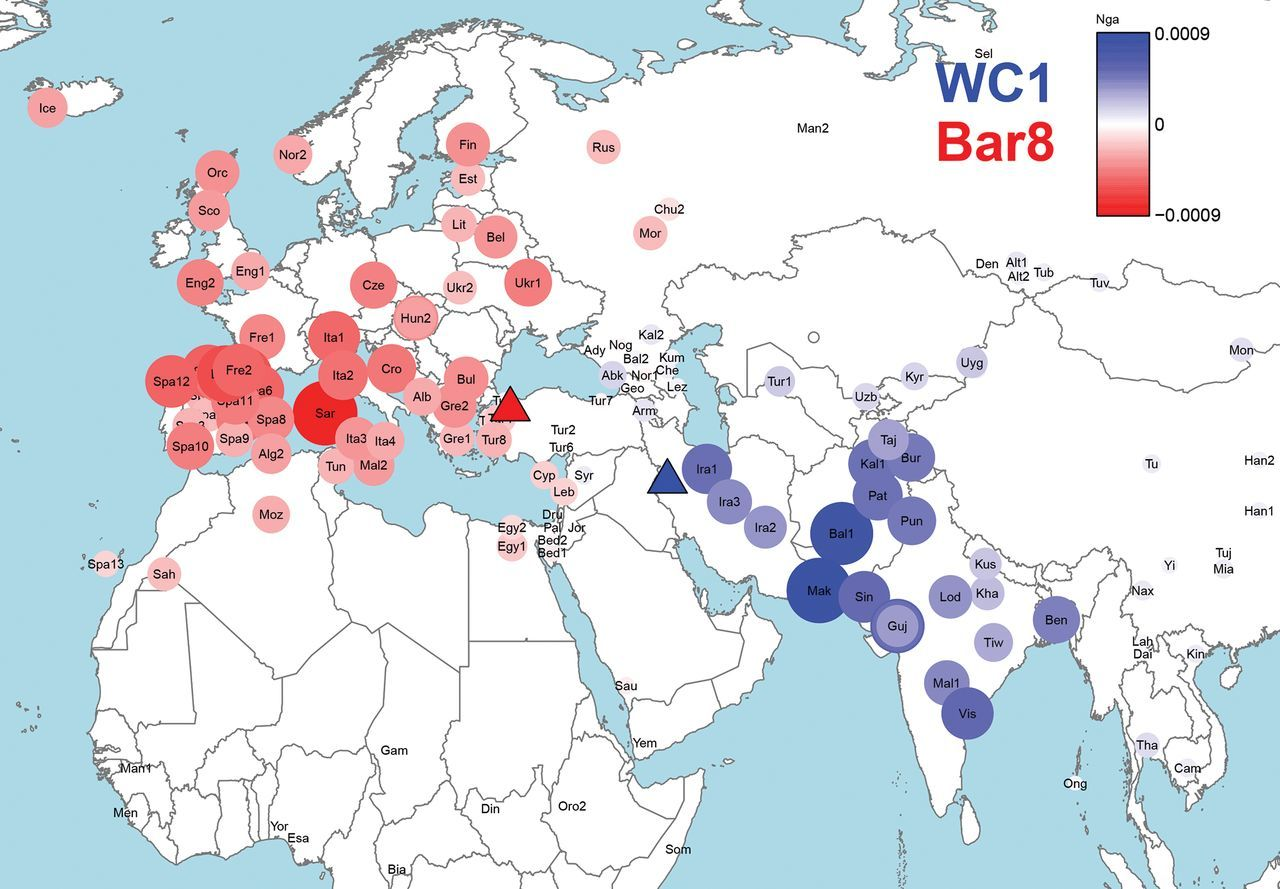
\includegraphics[width=1.0\textwidth]{../images/introduction/broushaki_haplotype_sharing.jpg}
    \caption{Map of differential haplotype sharing with present-day populations between WC1 (Iranian Farmer) and Bar8 (Anatolian Farmer) from Broushaki et al (2016) \cite{Broushaki2016a}. Bar8 copies relatively more from red populations and WC1 from blue populations.}
    \label{fig:broushaki_haplotype_sharing}
\end{figure}


The first use of ChromoPainter on ancient DNA was in the seminal paper of Lazaridis et al (2014) \cite{Lazaridis2014}. Through the generation of two high-coverage ancient genomes, they were the first to propose that most present-day Europeans can be modelled as a mixture of three ancestral populations. For the ChromoPainter analysis, they did not impute missing genotypes in the ancient samples, as the possible bias effects had yet to be studied; only positions with non-missing genotypes were retained. As the samples were of high coverage, this was not an issue, as 495,357 SNPs were kept. The the ability of fineSTRUCTURE to meaningfully cluster ancient individuals was confirmed by recapitulating previous results that identified different present-day European populations as being more closely related to Early Farmers and hunter-gatherers than others. 

In-between 2014 and the present-day, there have been approximately 31 studies which have used ChromoPainter on ancient samples (based on Web of Science search results). As of writing (September 2021), the study of Margaryan et al (2020) is the biggest so far to use ChromoPainter, with over 400 samples used \cite{margaryan2020population}. This study concluded that detecting structure within the dataset using `traditional' methods was not possible and so opted to use haplotype-based analyses on all samples above 0.5x mean depth. Another recent large study into the genomic history of the Roman Empire and surrounding regions leveraged ChromoPainter \cite{antonio2019ancient}.

More recently, ChromoPainter has been used to study aspects of archaic hominin ancestry in present-day humans \cite{JACOBS20191010, teixeira2021widespread}. Whilst ChromoPainter is not specifically designed to accurately estimate local ancestry, it is possible to infer identify potentially introgressed Denisovan regions of DNA by determining whether a haplotype which is more similar to the Denisovan genome than to a panel of sub-Saharan Africans. ChromoPainter has also been extended to studying the ancient DNA of non-human organisms such as bacteria \cite{Moodleye2015523118}. 

\subsubsection{Benchmarking ChromoPainter and imputation}

Many studies which have used ChromoPainter on ancient samples have performed tests and benchmarks to various degrees of detail. 

The first study to investigate the reliability of ChromoPainter on ancient DNA was Martiniano et al (2017) \cite{Martiniano2017}. Testing whether including imputed genotypes introduced bias towards particular present-day populations was key, as if it were the case, it may invalidate any results obtained. The authors estimated potential bias by plotting normal quantile-quantile plots of the copyvectors obtained from imputed (after downsampling to 2x coverage) and non-imputed markers. Whilst the differences in amount of copying differed by up to 14\%, most percentage differences were substantially lower and there was no evidence of structured bias towards or against particular geographic regions, with the authors concluding \blockquote{There is no strong evidence for systematic changes being caused by genotype imputation}.


The same study also investigated the impact of filtering genotypes based on genotype probabilities by creating two datasets, one containing filtered genotypes and without, and performing fineSTRUCTURE clustering on both. fineSTRUCTURE inferred 7 more clusters when using filtered genotypes; whilst this could be an indication of improved clustering resolution, it is hard to draw solid conclusions from these data. The overall number of fineSTRUCTURE clusters can not be seen as a direct measurement of performance; for example, the additional clusters inferred may simply be a result of the stochastic nature of MCMC sampling, and given only a single replicate of each test was performed, it is not possible to rule this out. Performing the same analysis on simulated data, where the population labels of individuals are known in advance, would be a more controlled test. 

Since the study of Martiniano et al, many papers which incorporated ChromoPainter analysis into studies of ancient DNA have included their own set of benchmarks. Antonio et al (2019) \cite{antonio2019ancient} tested imputation accuracy on an ancient sample (NE1) downsampled to different levels of coverage. However, this analysis was only performed on a single sample and the effect of imputation on the ChromoPainter process was not evaluated. Margaryan et al (2020) performed a downsampling test on two high coverage genomes down to 1x mean coverage and concluded that, whilst there was some suggestion that the 1x downsample tended to a more mixed ancestry profile, there was no evidence that incorrect ancestries have been inferred or that major changes in ancestries have occurred. 

Imputation is a necessary pre-processing step for ChromoPainter analysis on low-medium coverage ancient DNA samples for two primary reasons. Firstly, ChromoPainter does not allow for missing genotypes and so imputation is required to estimate missing genotypes. Secondly, whilst they are covered by reads, non-missing positions may still be low in coverage and thus require to be re-estimated, particularly when the true genotype is heterozygous. Therefore, it is important to determine to what extent it is possible to accurately impute genotypes at different levels of mean coverage. 

The accuracy of imputation on ancient samples has been tested in various studies \cite{Martiniano2017, hui2020evaluating, EmpiricalAncient}. There is difficulty in comparing the estimated accuracies between studies, however, due to differences in factors such as samples analyses, software used to call genotypes and impute samples, the regions analysed and filters applied. 

The most systematic and thorough evaluation of imputation in ancient genomes was performed by Hui et al (2020) \cite{hui2020evaluating}. This study noted that it is possible to impute using a one or two step approach and, through the use of downsampled genomes, showed that the two-step approach provides more accurate imputed genotypes. This study also showed that whilst most genotype likelihood callers (e.g. GATK, atlas) performed similarly well, atlas was preferred because of it's ability to model post-mortem damage (PMD) in ancient samples. Accordingly, I will use atlas to call genotype likelihoods in the rest of my thesis. 

It should be noted that the study only considered a single ancient genome (NE1) and it is therefore unclear how generalisable these results are to ancient samples of different ancestries. However, this study provided important benchmarks for many critical steps in the analysis of low coverage samples which had previously been missing from the literature, such as selection of a reference panel, the feasibility of local imputation and the effects of applying of pre and post imputation filters. One takeaway message was that it is possible to recover nine out of ten common (MAF $\geq$ 0.3) genotypes in a sample of 0.05x coverage. 

In Chapter 2 of my thesis, I will explore the effect of coverage on imputation and ChromoPainter performed on ancient DNA samples. 

\section{Issues and solution to low coverage data}

Low sequencing coverage is an issue which has plagued the field of ancient DNA since its inception. Compared to DNA obtained from present-day samples, ancient DNA samples typically have a much lower proportion of endogenous DNA, as DNA degrades over time from environmental factors. Therefore, when the DNA fragments are sequenced, relatively few of them will align to the human reference. 

The primary issue with low-coverage data is the increased uncertainty when calling diploid genotypes, particularly when the true genotype is heterozygous. Several methodological adaptations have been applied to existing methods in order to adapt them to low coverage ancient DNA. These approaches primarily attempt to circumvent making diploid genotype calls; for example, the previously mentioned strategy of pseudo-haploid genotype calling.

Alternatively, methods may avoid making diploid calls by working on genotype likelihoods. Genotype likelihoods represent a posterior estimate of the confidence of the three different genotypes at a bi-allelic locus, and thus allow the method to appropriately propogate that certainty throughout the analysis. A wide array of complex statistical approaches have been developed in order to accurately estimate the posterior genotype likelihoods. These approaches integrate factors such as sequencing-machine reported base-quality scores and estimates of read-mapping / sequencing errors \cite{McKenna2010}. Common methods to estimate likelihoods include the GATK model \cite{VanderAuwera2013}, SAMtools \cite{Li2009}, SOAPsnp \cite{Li2009a} and SYK model \cite{Kim2011}. Genotype likelihoods can either be estimated prior to the analysis from aligned reads (BAM files), using software such as ANGSD \cite{Korneliussen2014}, ATLAS \cite{Link2017} or GATK \cite{VanderAuwera2013}. Other softwares will take BAM files directly as input and estimate genotype likelihoods during the analysis process (e.g. STITCH \cite{Davies2016}). 

Once genotype likelihoods have been estimated, population level parameters such as inbreeding coefficients and $f_{st}$ can be estimated directly \cite{Korneliussen2014} with greater accuracy than direct genotype calls. Similarly, modifications of the ADMIXTURE \cite{Alexander2009} algorithm and PCA have been developed in order to analyse low coverage samples more effectively \cite{skotte2013estimating, zhang2021novel}. Recent advances have allowed the identification of 1st and 2nd-degree relatives from as low as 0.02x coverage samples \cite{fernandes2017identification, fernandes2021tkgwv2}. 

Several methods account for low-coverage data by jointly estimating ancient DNA specific confounding factors, such as contamination and  post-mortem damage, alongside the demographic parameter of interest \cite{Racimo2016}. For instance, Schraiber (2018) \cite{Schraiber2018} developed a novel maximum-likelihood approach which leverages information from different low-coverage samples from within the same population to infer population-level parameters, such as genetic continuity between ancient and modern populations.  

Viera et al (2016) developed a method (ngsF-HMM) to infer matching identical-by-descent (IBD) segments from low-coverage data \cite{Vieira2016}. To account for the uncertainty, all three genotype likelihoods are integrated over in order to estimate whether or not a genomic region is IBD given the likelihoods. This method showed that there is a substantial gain in power when likelihoods are used compared to genotype calls.  

As mentioned in the previous paragraph, there are several other characteristics of ancient DNA which should be accounted for when performing genetic analysis. 

Present-day humans contaminating ancient genetic samples is of primary concern as it non-trivial to distinguish between sequencing reads originating from the ancient sample and e.g. present-day individuals performing laboratory analysis \cite{peyregne2020present}. A failure to account for such contamination may lead to underestimating the level of divergence between present-day and ancient samples, as well as the introduction of spurious signals of admixture \cite{Green2010, wall2007inconsistencies, green2009neandertal}. In addition to the many precautions taken in the laboratory to reduce the risk of human contamination, such as performing analysis in positive-pressure rooms and intensive irradiation of equipment, several bioinformatics approaches have also been developed to estimate the level of contamination in an ancient sample. For example, a recent method leveraged the fact that contaminating sequences are found on different haplotypes to the genuine ancient sequence and so can be detected through a reduction in local levels of linkage disequilibrium relative to those found in a reference panel\cite{nakatsuka2020contamld}. As contaminant sequences are more likely to carry a derived allele \cite{peyregne2020present}, searching the genome for significant deviations from the expected equilibrium percentage of dervied allele (0\% at homozygous ancestral and 50\% at heterozygous sites) allows for the estimation of local contamination rates \cite{Green2010, Meyer2012}. 

Another aspect of ancient DNA that must be considered is that of post-morterm degradation (PMD). For example, DNA fragmentation (hydrolytic depurination resulting in single-strand breaks) means nearly all ancient DNA fragments are between 40-500bp in length \cite{paabo1989ancient, paabo1991miocene}. The presence of substantially shorter DNA fragments increases the risk of mis-aligning reads to the incorrect part of the genome \cite{de2018quantifying}.

Further, intermolecular cross-links can form between DNA strands \cite{paabo1989ancient} and miscoding lesions, caused by hydrolytic deamination of nucleotides, may result in modifications that cause nucleotides to be misread by DNA polymerases \cite{dabney2013ancient}. One consequence of this is that it leads to an excess of spurious C->T substitutions after sequencing \cite{paabo1989ancient}. Failing to account for such substitutions (usually termed cytosine deamination) may lead to downstream errors in bioinformatic analyses. Therefore, methods have been developed in order to account for cytosine deamination; for example, the atlas suite of tools which are specifically designed to call variants in low-coverage ancient DNA samples \cite{Link2017}. atlas  takes advantage of the fact that cytosine deamination is more likely to occur at the beginning of a sequencing read to model the extent of PMD using an exponential decay function (decaying exponentially with respect to the position on the sequencing read). This provides a likelihood that a given C->T substitution is a true mutation or the result of PMD. Integrating this model into the variant-calling process resulted in a subsantially higher proportion of correctly called genotypes relative to an ancient DNA-naive method (GATK) \cite{Link2017}. 


In this thesis, I will attempt to mitigate any effects of low-coverage data on ChromoPainter analysis by implementing an approach similar to that of Viera et al (2016), which modifies the ChromoPainter algorithm to account for genotype likelihoods.


\section{Combining data from multiple chips}

An issue similar to that of low-coverage ancient DNA data stems from the development of a large number of different genotyping arrays. Different cohorts are genotyped on different arrays and sets of SNPs, as different SNPs have different characteristics, such as different frequencies in different populations and associations with different phenotypes. Whilst this has meant a wider variety of questions and populations can be studied, it also makes combining data from across different arrays potentially troublesome, as they often have a small overlap in the SNPs upon which they have been genotyped.

For example, in my thesis, I have worked with at least three genotyping arrays, referred to here as `Human Origins', `Hell Bus' and the UK Biobank. Often I have wanted to compare populations on different arrays, such as the African populations on the Human Origins array and UK Biobank individuals on the UK Biobank array. After merging the datasets, the overlap was small, only 70,000 SNPs. This is around an order of magnitude fewer SNPs than is analyse a typical ChromoPainter analysis. Having fewer SNPs may reduce power, as there are fewer pieces of information, and less linkage between each neighbouring SNP.

One solution to the issue of a small number of SNPs would be to impute the remaining SNPs using a reference panel and imputation algorithm such as Beagle \cite{Browning2016}. However, it is possible that imputation may cause a bias in the data. If missing genotypes are imputed incorrectly more often from one population than another, this will result in an increased, but spurious genetic similarity between the target and reference population. This may be a particular issue when analysing populations which are not well represented in imputation reference panels, such as non-Europeans. The nature and magnitude of this bias, however, is yet to be fully understood, particularly in the context of ChromoPainter.  

Therefore, this thesis will explore whether is it more desirable to impute the missing positions or to use use a smaller number of overlapping SNPs. Accordingly, in chapter 3 of this thesis, I will explore this question with a case study investigating African ancestry in the UK Biobank dataset. 
 
\section{Summary of thesis aims}

In this thesis I will explore the applicability of ChromoPainter to low-coverage ancient DNA samples and sparsely genotyped data resulting from merged genotype arrays. To do this, I will perform a series of tests on both real and simulated data from present-day and ancient samples and apply my findings to two novel (unpublished) datasets of ancient samples from Bavaria and Czechia. 

Specifically, in Chapter 2, I will perform downsampling simulations on five high-coverage ancient genomes to assess the impact of coverage on imputation, phasing and ChromoPainter analysis, and determine the feasibility of extracting haplotype information from sparsely genotyped data in practice. In Chapter 3, I will infer African ancestry across samples in the U.K. Biobank dataset, using sparsely genotyped data resulting from the merge of two different genotyping arrays. I will investigate the potential of using imputation to boost power to infer fine-scale ancestry signatures in U.K. Biobank participants, in terms of how closely related they are to individuals in reference data containing a large number of African ethnolinguistic groups. In Chapter 4, I will analyse unpublished ancient genome data from Bavaria, obtained by collaborators at Mainz University, exploring how genetic patterns varied from the Neolithic to the Medieval Era in a small geographic region. In Chapter 5, I will analyse unpublished ancient Slavic samples from Czechia, obtained by collaborators at Max Planck Institute for Evolutionary Anthropology, to assess the genetic relationships between Migration Era, Middle age and present-day Slavic-speaking peoples. Lastly, my concluding chapter will summarise my work and key findings, including my recommendations for future haplotype-based studies using low-coverage data and/or combining data from multiple SNP arrays.





\chapter{ChromoPainter and ancient DNA}
\label{chapterlabel2}

\section{Introduction}

This chapter is related to the use of ChromoPainter on low coverage ancient DNA samples. 

First, I will describe the existing methodology, ChromoPainterV2, and then a new version I have developed, ChromoPainterUncertainty, which is designed to mitigate bias related to sequencing coverage. 

Next I will perform benchmarking tests on all the steps necessary to analyse low-coverage ancient DNA with ChromoPainter. This includes genotype calling and genotype likelihood estimation with atlas \cite{Link2017}, phasing and genotype imputation with GLIMPSE \cite{rubinacci2021efficient}, ChromoPainter \cite{Lawson2012} analysis (copy-vector estimation and PCA) and SOURCEFIND ancestry component estimation \cite{Chacon-Duque2018}. I will also describe some of the existing issues pertaining to low coverage ancient DNA and several considered mitigation strategies. Finally, I will simulate, using present-day samples, ancient samples with variable degrees of missing SNPs in order to determine whether ancient samples of a particular coverage have enough typed SNPs to retain haplotype information.   

\section{Methods}

\subsection{Description of the ChromoPainter algorithm} \label{sec:ChromopainterDescription}

As discussed in the introduction, ChromoPainter is a method designed to estimate the amount haplotype sharing between individuals \cite{Lawson2012}. In diploid organisms such as humans and dogs, ignoring copy-number-variation, each autosomal region of an individual is represented by two haplotypes. As input, ChromoPainter requires each individual's data to be `phased' into these two haplotypes. Phasing refers to the process of determining which alleles along a chromosome were inherited together from the same parent. 

In ChromoPainter, sampled individuals are split into `donor' and `recipient' haplotypes. It employs the widely-used Li and Stephens copying model \cite{Li2003} to model each recipient haplotype as a mosaic of all haplotypes observed in the donor panel. Typically (and throughout this thesis) an individual does not act as a donor to themself, e.g.\ one of the individual's two haplotypes can not act as a donor for the other haplotype. Unlike the original Li and Stephens model, which uses the product of approximate conditionals (PAC) likelihoods, ChromoPainter reconstructs each recipient haplotype as a mosaic of \textit{all} other donor haplotypes. Here, the term `copying' can be though of as a genealogical process where haplotypes are reconstructed using the genealogically closest haplotype in the donor set.  

Suppose we have a particular recipient haplotype, $h*$, which consists of a sequence of $L$ alleles denoted by $\{h*_{1}, ..., h*_{L}\}$, where $h*_{l}$ is the observed allele at site $l$. We wish to paint $h*$ using $j$ donor haplotypes, denoted by $\{h_{1}, ..., h_{j}\}$. 

The copying model is implemented in the form of a Hidden Markov Model (HMM), with the observed states being the alleles carried by the donor and recipient individuals, and the hidden states being the `nearest-neighbour' haplotype the recipient haplotype $h*$ copies from. Thus we can define a hidden-state sequence vector $\{Y_{1}, ..., Y_{L}\}$, which corresponds to which of the $j$ donors $h*$ copies from at a given site $l$. The emission probabilities are given as the probability of $h*$ carrying allele $a$ at site $l$, given it copies from donor haplotype $y$ and $h_{yl}$ is the allele carried by donor haplotype $y$ at site $l$. This probability is conditional upon whether, $h*$ and $y$ both carry allele $a$ at site $l$ or not:

\begin{equation} \label{eq:cp}
\Pr(h*_{l} = a \mid Y_{l} = y) =     
	\begin{cases}
		1.0 - \theta & h_{yl} = a; \\
		\theta & h_{yl} \neq a. 
	\end{cases}       
\end{equation}

where $\theta$ is the probability of a mutation occurring. The mutation probability $\theta$ can be estimated using Watterson's estimator \cite{Watterson1975}, or estimated using an iterative EM algorithm.

The transition probabilities of the HMM, which are the probabilities of a change in the donor being copied from when transitioning from one SNP to another, is guided by a recombination rate map, with higher recombination rates leading to a higher probability of transitioning. Switches between donors are interpreted as changes in ancestral relationships due to historical recombination and modelled as a Poisson process. 

In ChromoPainterV2, the input genetic data comes in the form of phased genotype calls (i.e. \texttt{1|0}). ChromoPainterV2 produces several different output files. The two which most used in this work are those appended with .chunklengths and .chunkcounts. These matrices are also referred to as `coancestry matrices'. In the chunklengths matrix, $cl$, the entry $cl_{d,r}$ gives the total expected proportion of haplotype segments (defined as a contiguous set of SNPs copied from a single donor) that recipient $r$ copies from donor $d$. Thus, higher values of $cl_{d,r}$ indicate that recipient $r$ and donor $d$ share more recent ancestry. The .chunkcounts matrix instead gives the total number of haplotype segments that recipient $r$ copies from donor $d$.

In this work, `copyvector' is used to refer to the vector of chunklengths that a single recipient individual copies from all donors, or a single row of the coancestry matrix. Throughout, I often define donors as populations, so that{ each element of the copy vector is the total amount of DNA that the recipient matches to all individuals from a given donor population.

\subsubsection{Description of ChromoPainterV2Uncertainty} \label{sec:DescriptionChromoPainterV2Uncertainty}

ChromoPainterUncertainty works in a very similar way to ChromoPainterV2, bar two differences. Firstly, the input data is in the form of an allele probability $0 \leq x \leq 1$, which is given as the probability of observing the alternate allele at that SNP. This value is calculated from the posterior likelihood that an allele has been imputed correctly. This is different to ChromoPainterV2, which uses `hard' allele calls that only take a value of 0 or 1.

Here, I will show how it is possible to incorporate the uncertainty in imputed genotype calls into the ChromoPainter input. Consider the following example: we have a phased genotype in the form \texttt{0|1}, corresponding to the reference allele on the first haplotype and the alternative allele at the second haplotype. I define $G$ as the sum of the genotypes at a SNP; in this case $G=0+1=1$. As GLIMPSE, the imputation and phasing algorithm I will use for this work, provides hard genotype calls, $G$ can be calculated directly.

We also have a posterior genotype likelihood, in the form $GL(p_{0}, p_{1}, p_{2})$, where $p_i$ is the posterior probabilities that the true genotype is $i$. Genotype probability dosage, $D$, is the expected total number of copies of the alternate allele given $GL$. $D$ can be calculated as $p_{1} + [2*p_{2}]$. We can calculate $U$, the uncertainty as $U = |G-D|$. Then, we can assign a probability to each allele; if the allele is \texttt{1} then the allele likelihood is simply $1 - U$ and if the allele is \texttt{0} then the allele likelihood is $0 + U$. Therefore, when there is no uncertainty in the genotype call, the allele probability will be either 0 or 1. When there is uncertainty, the allele probability will take a value $0 \leq x \leq 1$, with more uncertain genotypes tending towards allele probabilities of 0.5. 



                 
The second difference is the incorporation of the allele probability into the emission probability of the HMM. As before, consider a recipient $h*$ whom we want to paint using the set of donors $\{h_{1}, ..., h_{j}\}$ . At a given SNP $l$, let $h*_{l}$ be the probability that $h*$ carries the alternative allele, with $h_{yl}$ similarly being the probability that donor haplotype $y$ carries the alternate allele at position $l$. The probability of $h*$ carrying allele $a$ at site $l$, given it copies from haplotype $y$ is given as:

\begin{align} \label{eq:cp_uncertainty}
\begin{split}
	\Pr(h*_{l} = a \mid Y_{l} = y) = &
				\,(1 - \theta) \cdot [a \cdot h_{yl} + (1-a) \cdot (1-h_{yl})]\, +  \\
				& \theta \cdot [a \cdot (1-h_{yl}) + (1-a) \cdot h_{yl}]
\end{split}
\end{align}

Note that equation \ref{eq:cp_uncertainty} reduces to equation \ref{eq:cp} if $h_{yl} = \{0,1\}$ and if $a = \{0,1\}$, i.e\ there is no uncertainty in the calls.

A consideration of a different uncertainty metric, $max(GP)$, can be found in Appendix section \ref{sec:alt_input_score_test}.


\subsection{Generation of downsampled genomes}

 I created a set of `downsampled' ancient genomes in order to explicitly quantify the effect of coverage on each stage of the ChromoPainter analysis. I took five high coverage genomes and for each, removed a random subset of reads from the \texttt{.bam} file in order to reduce the coverage to a target level. I then performed each stage of a typical ChromoPainter analysis, e.g.\ mimicking the analyses of new ancient DNA samples I describe in chapters 4 and 5, on the full coverage and downsampled genomes. I also processed a set of 918 ancient samples from the literature, downloaded from the European Nucleotide Archive, in an identical way to act as comparison samples (Section \ref{sec:ancient_ref_samples}).

Five high coverage ancient genomes were downloaded in the form of aligned \texttt{.bam} files from the European Nucleotide Archive:

\begin{enumerate}
\item Yamnaya (25.2x) -- Yamnaya Bronze Age steppe-pastoralist \cite{deBarrosDamgaardeaar7711}
\item UstIshim (42x) -- Siberian Upper Palaeolithic hunter-gatherer \cite{Fu2014}
\item sf12 (72x) -- Scandinavian Hunter-Gatherer \cite{Gunther2018a}
\item LBK (19x)-- early European farmer from the \textit{Linearbandkeramik} culture from Stuttgart, Germany \cite{Lazaridis2014}
\item Loschbour (22x) -- 8,000 year-old hunter-gatherer from Luxembourg) \cite{Lazaridis2014}
\end{enumerate}

These samples were chosen due to their high original coverage ($>18$x), and because they represent some of the ancestries present in Western Eurasia over the past 40,000 years.  

For each full coverage, downsampled and literature ancient \texttt{.bam} file was processed using the atlas (version 1.0, commit f612f28) pipeline \cite{Link2017} \\(\url{https://bitbucket.org/wegmannlab/atlas/wiki/Home}). First, the validity of each file was assessed (i.e. ensuring that each \texttt{.bam} file was not malformed in any way) using ValidateSamFile command from PicardTools \cite{Picard2018toolkit}. atlas is a suite of software designed for processing low-coverage ancient DNA and was chosen following the recommendation of Hui et al (2020) \cite{hui2020evaluating}, as it explicitly accounts for post-mortem damage (PMD) patterns in ancient DNA. The most common form of PMD is C-deamination, which leads to a C->T transition on the affected strand and a G-->A transition on the complimentary strand.

I then downsampled each full-coverage genome using the \texttt{atlas downsample} task, resulting in a \texttt{.bam} file with coverages 0.1x, 0.5x, 0.8x, 1x, 2x, 3.5x, 5x, 10x and 20x per individual. 

Again, for each full coverage, downsampled and literature ancient \texttt{.bam} file, I estimated post-mortem damage (PMD) patterns using the \texttt{atlas estimatePMD} task. Recalibration parameters were then estimated using the atlas \texttt{atlas recal} task. Finally, both the recalibration and PMD parameters were given to the \texttt{atlas callNEW} task which produces genotype calls and genotype likelihood estimates for each downsampled and full coverage \texttt{.bam}. For this stage, I made calls at the 77,818,264 genome-wide positions present in the phase 3 thousand genomes project \cite{1000GenomesProjectConsortium2015}. This was done to reduce the risk of calling false-positive (i.e.\ falsely polymorphic) genotypes in the aDNA samples. No minimum read-depth filter was applied when calling genotypes. This step resulted in a \texttt{.vcf} file for each of the samples. For each of the 22 autosomes, I merged all samples together into a single \texttt{.vcf} file. 

atlas does not make calls at positions in the genome where no reads have been aligned. If multiple \texttt{.vcf} files are merged together, and at a given position in the genome, some samples contain genotype calls and others do not, this position will be present but the genotype will be set as missing \texttt{./.} in  the merged \texttt{.vcf}. Therefore, the merged \texttt{.vcf} contained positions at all 77,818,264 positions, as across all X samples, at least one individual have a genotype call at each position. 


\begin{figure}[htp]
    \centering
    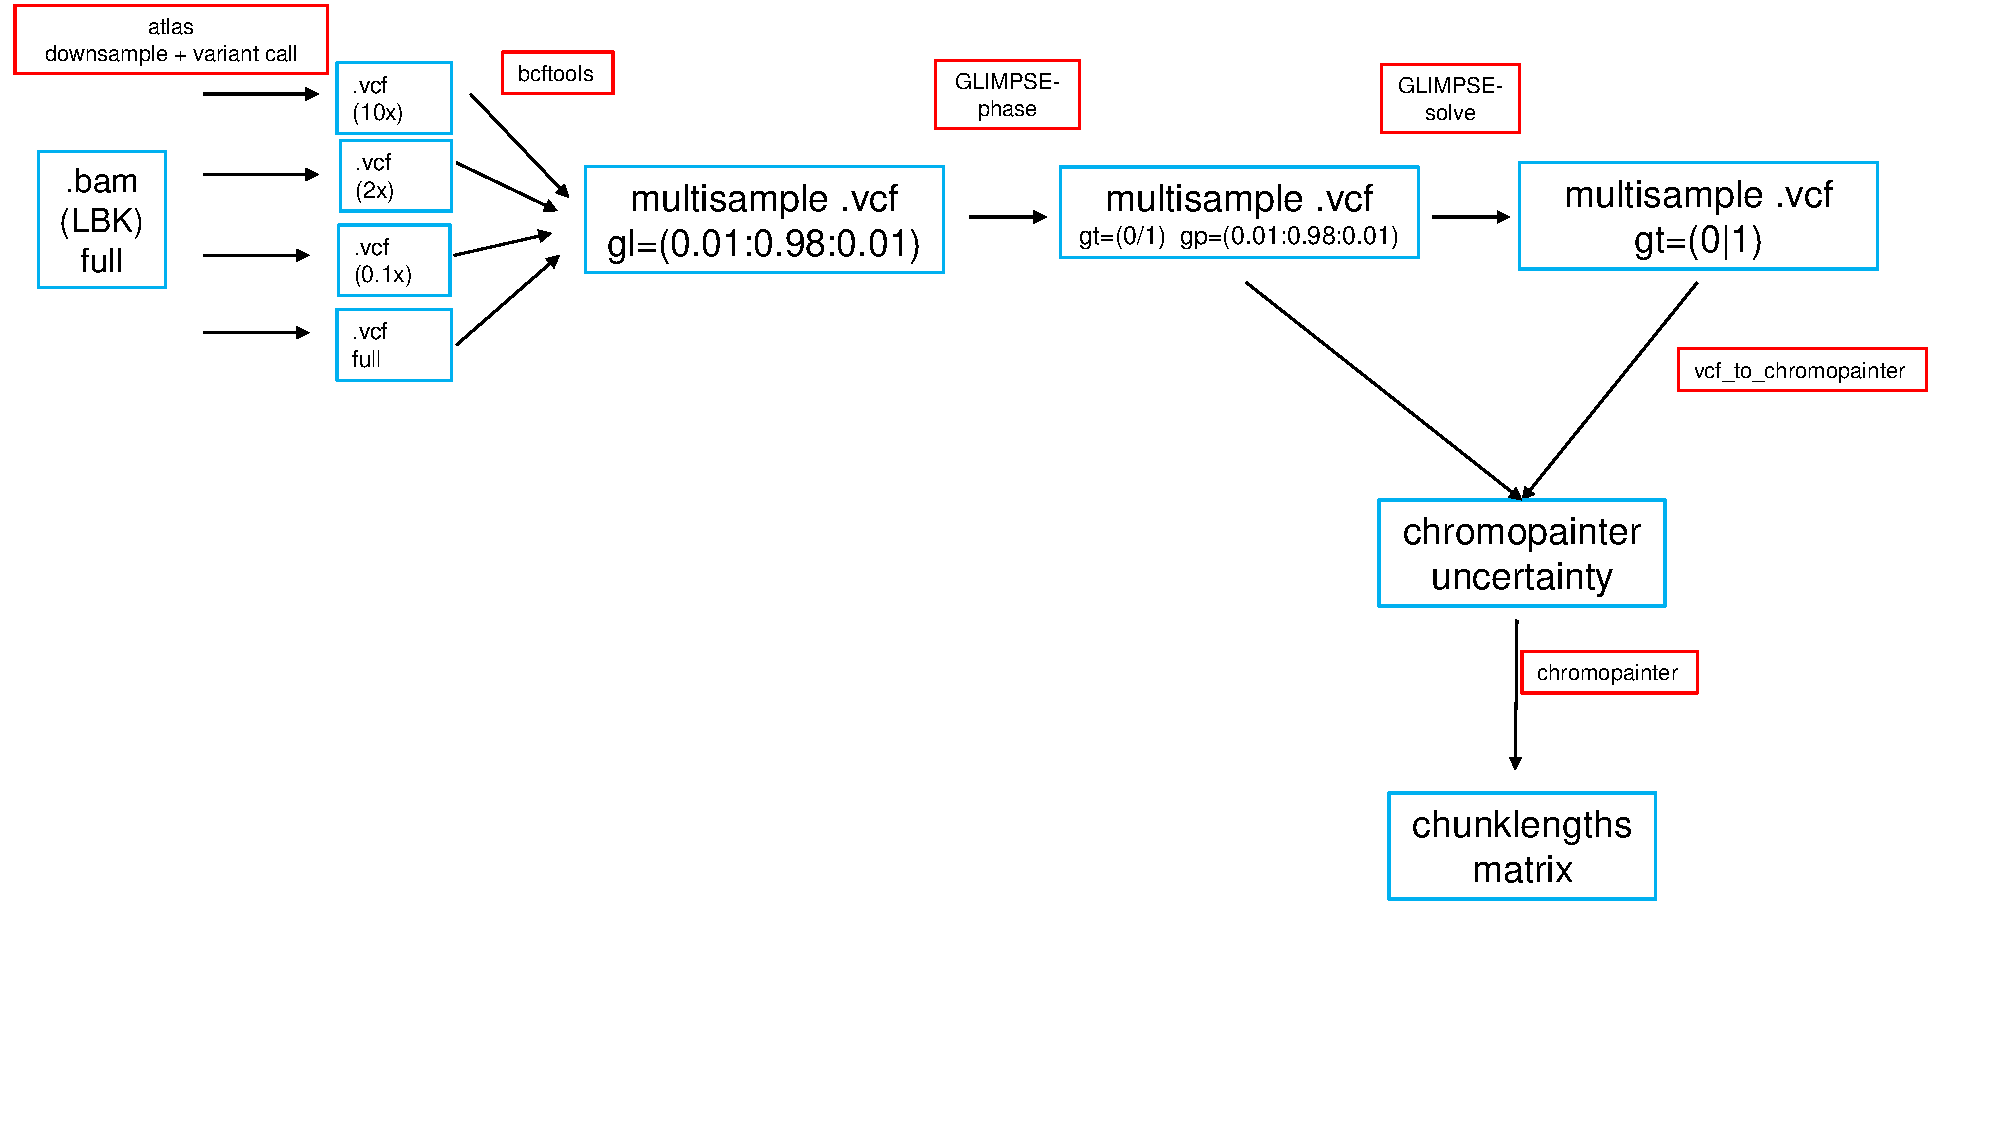
\includegraphics[width=1.0\textwidth]{../images/chapter1/workflow.pdf}
    \caption{Schematic showing the workflow used to generate downsampled ancient genomes. Blue boxes represent the genetic data in different formats and red boxes represent methods used to process data or convert between formats. Schematic shows a reduced example of LBK being downmsapled to 3 different coverages. A high coverage .bam file is downsampled used to generated genotype likelihoods in .vcf format using atlas \cite{Link2017}. GLIMPSE is used to impute and phase the .vcf, producing posterior genotype probabilities and phased genotypes. These are combined using a custom script to generate ChromoPainter uncertainty output.}
    \label{fig:Sensitivity_downsampled_rtgtools}
\end{figure}

\subsection{Generation of ancient literature samples} \label{AncientReferenceSamples}

I also generated a set of ancient samples from the literature to use as donors in the ChromoPainter analysis.

This dataset consists of 918 other ancient samples from the literature given in Appendix section \ref{section:AncientReferenceDataset}. These samples were of variable coverage, ranging from 0.002-72x coverage, and chosen because of their previously reported relevance to understanding past ancestry patterns in European populations like those analysed in chapters 4 and 5. These 918 consist of all samples given in Table \ref{tab:AncientReferenceDataset} were processed in an identical way to the downsampled target individuals described in the previous section, other than they were not downsampled.  

\subsection{Imputation and phasing - GLIMPSE}

Genotype imputation and phasing are two important steps for processing low-coverage ancient DNA. Low coverage ($<$1x) samples typically lack enough read information to make accurate genotype calls at most positions in the genome, and often do not contain any reads at many positions \cite{nielsen2011genotype}. Therefore, it can be helpful to use external information from a high-coverage reference panel in order to improve the accuracy of genotype calls and phasing, reducing the impact of errors on downstream analyses \cite{rubinacci2021efficient}. 

Three different characteristics are desirable for an imputation algorithm in this context. Firstly, it should take genotype likelihoods as input. This is because genotype likelihoods allow for flexible representation of the possible genotypes at a particular position, particularly when there may not be enough coverage to make a hard genotype call. Secondly, it should emit posterior genotype-probabilities which, when accurately calibrated, give the probability that a particular genotype call is correct. This is necessary for estimating the uncertainty values, described in section \ref{sec:DescriptionChromoPainterV2Uncertainty}, needed for ChromoPainterUncertainty analysis. Thirdly, the algorithm must be able to complete in a reasonable running time when using a large number of samples and high number of SNPs. Using a large number of densely positioned SNPs (e.g. such as the approximately 77 million identified in the 1000 Genomes Project) increases the useful linkage-disequilibrium information between each SNP, and it is well-established that increasing the number of individuals used in imputation/phasing reference panels improves accuracy \cite{delaneau2018integrative, HUANG2009235, mccarthy2016reference, rubinacci2021efficient}. 

Two programs, Beagle 4.0 \cite{Browning2007} and GLIMPSE \cite{rubinacci2021efficient} fulfil the first and second criteria above, but GLIMPSE offers up to 1000x reduction in running time compared to Beagle 4.0 \cite{rubinacci2021efficicanent}, and hence chose it for the imputation and phasing steps.   

Phasing and imputation ideally requires a reference panel of high-coverage present-day individuals. I used the 1000 Genomes Project dataset re-sequenced to 30x average coverage, which contains 3202 individuals from 26 worldwide populations \cite{byrska2021high}. A description of the processing of this reference dataset can be found in Appendix \ref{section:1000genomes}. This reference dataset contained 50,509,915 unique bi-allelic SNPs. 

I merged together i) the full coverage individuals, ii) downsampled individuals and iii) 918 ancient samples from the literature into a single bcf file using bcftools (version 1.11-60-g09dca3e) \cite{li2011statistical} to act as the samples for GLIMPSE to phase. Here, `target' refers to the individuals being imputed/phased and `reference' refers to the reference panel.  

Following the GLIMPSE tutorial (\url{https://odelaneau.github.io/GLIMPSE/tutorial_b38.html}), I first used \texttt{GLIMPSE\_chunk} to split up each  chromosome into chunks, keeping both \texttt{--window-size} and \texttt{--buffer-size} to 2,000,000 base pairs, which is their default settings. I used the b37 genetic map supplied by GLIMPSE for the \texttt{--map} argument. Across all chromosomes, this produced 936 chunks that are on average 2.99Mb long. 

GLIMPSE then imputed each chunk separately, using \texttt{GLIMPSE\_phase} using the same 1000 genomes dataset as a reference and default settings. This stage both imputes missing genotypes and generates a set of haplotype pairs which can be sampled from in a later step to produce phased haplotypes. \texttt{GLIMPSE\_ligate} then merges the imputed chunks back to form single chromosomes using the default settings. I then used \texttt{GLIMPSE\_sample} to produce a .vcf with phased haplotypes sampled for each individual, again using default settings. Consequently, the output of GLIMPSE is i) unphased genotype calls with posterior genotype likelihoods and ii) phased haplotypes.

It is important to note that GLIMPSE leverages information from individuals that have been imputed, `absorbing' them into the reference panel. For example, if there were 100 target samples and 1000 reference samples, each target is phased in turn and then absorbed into the reference panel, so that there would be 1001 reference samples when the second target individual is imputed. This makes it necessary to avoid including the same sample, downsampled to different coverages, in the same set of targets for one imputation run, in order to avoid the confounding effect of allowing an individual to act as the reference to itself. For example, including Loschbour at 0.1x and 10x coverage could mean it imputed itself, a situation which would never occur in reality. 


\subsection{Estimating imputation sensitivity and specificity}

I used rtg-tools-3.11 \cite{cleary2014joint} and the \texttt{vcfeval} task to estimate the sensitivity and specificity of imputation in the downsampled individuals. Here, `baseline' (i.e. the truthset) is defined as the genotype calls in the full coverage individual and the `calls' as the genotype calls in the downsampled individual. Sensitivity and precision are defined as: 

\begin{equation}
sensitivity = \frac{V_{call}-FP}{V_{call}}
\end{equation}

\begin{equation}
precision = \frac{V_{baseline}-FN}{V_{baseline}}
\end{equation}

A `variant' is considered to be a SNP with a genotype that is either \texttt{0/1} or \texttt{1/1}, with $V_{baseline}$ and $V_{call}$ the number of variants called in the full coverage and downsampled genomes, respectively. False negatives (FN) are where a variant is called in the full coverage genome but not in the downsampled genome. False positives (FP) are cases where a variant is called in the downsampled genome but not in the full-coverage genome.

$V$, or true-positive, is the number of events where a variant position (i.e. a SNP with a genotype that is either \texttt{0/1} or \texttt{1/1}) is detected in either the full coverage ($V_{baseline}$) or downsampled ($V_{baseline}$) sample. $FN$ is the number of times that a variant position is called in the full coverage sample and not the downsampled sample. Conversely, $FP$ is the number of times a variant position is called in the downsampled sample and where the same SNP in the full coverage sample is invariant (i.e. \texttt{0/0}). Only genotypes called in the full coverage and downsampled individuals were considered. No allele frequency filters were applied before conducting this analysis.

\subsection{ChromoPainter analysis} \label{ChromoPainter_analysis}

It is important to understand the effect of sequencing coverage on the accuracy of ChromoPainter copyvector estimation. A `copyvector', $c_{r}$, is a vector of length $D$, where each entry gives the total length of genome that recipient individual $r$ most closely matches to each of the $D$ donor individual/populations. I sometimes refer to `normalised' copyvectors; this simply refers to where each entry of $c_r$ is divided by the sum of all entries, scaling the copyvector to sum to 1. 

I painted each downsampled and full coverage ancient individual using a set of 124 ancient individuals, hereafter referred to as the `standard set', selected because they had a sequencing depth greater than 2x. I compared the copyvectors for the same individual at each level of downsampling, to the same individual at full coverage. For example, I compared the copyvector of Yamnaya at 0.1x to the copyvector of the same Yamnaya sample at full coverage. A high correspondence, measured by r-squared for example, between the copyvectors of the full coverage and downsampled individual suggests less effect of coverage. 

To prepare the data for ChromoPainter, I merged the .vcf containing the posterior genotype likelihoods of i) downsampled, ii) full coverage and iii) 124 ancient samples from the literature together, and did the same for the .vcfs containing the phased haplotypes.  I combined the posterior genotype likelihoods with the phased alleles to generate allele likelihoods (described in section \ref{sec:DescriptionChromoPainterV2Uncertainty}) in ChromoPainter-uncertainty format, in addition to per-position recombination rate files. This was performed for each chromosome in turn using my own script (\url{https://github.com/sahwa/vcf_to_ChromoPainter}).

I next used ChromoPainterUncertainty to perform the painting. I assigned the standard set individuals as donors and all downsampled, full coverage and standard set as recipients. The `standard set' samples from the literature were included in order so that they can be used a surrogates in later SOURCEFIND analysis.

I also performed an identical analysis, but using ChromoPainterV2 and hard genotype calls. 

This painting produced a chunklengths matrix for each chromosome which were merged using chromocombine-0.0.4 (\url{https://people.maths.bris.ac.uk/~madjl/finestructure-old/chromocombine.html}). The resulting chunklengths matrix thus gives the total length of genome in centimorgans that a recipient most closely matches to each donor individual. 

\subsection{ChromoPainter Principle Component Analysis}

Principle Component Analysis (PCA) can be used to reduce the underlying structure in the chunklengths coancestry matrix to two dimensions, thus allowing it to be more easily visualised. As individuals cannot paint themselves, the diagonals of each coancestry matrix contain zeros. Therefore, I performed PCA using the fineSTRUCTURE library \url{https://people.maths.bris.ac.uk/~madjl/finestructure/finestructureR.html}.

All downsampled and full coverage individuals were projected onto the principle components of the reference ancient samples. 


\subsection{SOURCEFIND}

The chunklengths coancestry matrix produced by ChromoPainter contains information about the estimated length of genome a recipient most closely matches a given donor individual or population. However, incomplete lineage sorting, where alleles segregate in a way that is discordant to the true phylogeny reflecting the orders in which populations split from one another, means that there are regions in the genome where a recipient individual most closely matches a reference individual that is not from their own population. For example, an individual from France copies non-zero amounts from African donors, despite not having any African ancestry through recent admixture. Furthermore, unequal donor population sizes may bias the aggregated amount copied to a given population. 

Therefore, to account for these issues when estimating ancestry proportions, it is necessary to run an additional step, SOURCEFIND \cite{Chacon-Duque2018}. Simulations have shown that SOURCEFIND ancestry proportions correspond well to simulated truth-set values \cite{Chacon-Duque2018}. The ancestry proportions produced by SOURCEFIND should be interpreted as the proportion of ancestry that each individual/population shares most recently with each surrogate. This need not necessarily imply an admixture event; for instance, you might expect $France$ to have ancestry recently related to both $Germany$ and $Spain$ due to isolation-by-distance rather than admixture. 

SOURCEFIND models each target copyvector as a linear mixture of copyvectors from a set of surrogate groups, inferring the proportion of ancestry for which the target individual is most recently related to each surrogate group. The parameter space of surrogate ancestry proportions is explored using a Markov chain Monte Carlo algorithm, where the ancestry proportions are updated using a Metropolis-Hastings step. The output of SOURCEFIND for each target individual is therefore an $n*p$ matrix, where $n$ is the number of MCMC samples and $p$ is the total number of surrogate groups. 

To test for the effect of coverage on the proportions estimated by SOURCEFIND, I performed two separate analyses, both using the downsampled and full coverage individuals as targets. The first uses three surrogate populations (Yamnaya, Western Hunter-Gatherer and Anatolia Neolithic Farmer), and the second uses an expanded list of 37 surrogate populations. I chose the first set of three surrogates, as these are typically used in ancient DNA analysis to obtain a 'broad' overview of the ancestry of a European individual, as it has been shown that central Europeans within the last 10,000 years can be well modelled as a mixture of those three groups \cite{Lazaridis2014, Haak2015}. Note, this does not mean that there was not admixture from other sources, but that a majority of ancestry of ancient central Europeans can be derived from these sources. This stands to act as a relatively straightforward test case, since the three populations are highly genetically differentiated from one another.

For all runs of SOURCEFIND, I used 1,000,000 iterations, of which 50,000 were designated as burn-ins, and then samples were taken every 50 iterations. 2,000,000 iterations were chosen because my previous tests show that is the minimum necessary to provide reasonably confidence of convergence within reasonable running time (Appendix section \ref{sec:SF_test_iterations}). The rest of the parameters were left as default. Ancestry proportions and credible intervals group were estimated using the CODA R library \cite{oro22547}.

\section{Pre-post GLIMPSE and linked/unlinked PCA test}

I wanted to determine at what stage of the analysis pipeline low coverage samples (0.1x) significantly diverge from the other downsamples when plotted on a PCA. I will hereafter refer to this phenomenom as `coverage-related bias'. For instance, it may be that the coverage-related bias is introduced in the imputation stage. Coverage-related bias can be measured by calculating $d = \sqrt{(PC1_{f} - PC1_{d})^2 + (PC2_{f} - PC2_{d})^2}$, where $(PC1_{f}$ is the PC1 value for the full coverage individual and $(PC1_{d}$ is the equivalent for the downsampled individual. In other words, $d$ measures the Cartesian distance between the full coverage and downsampled individual on principle component space, with higher distances corresponding to more coverage-related bias. 

To test this, I performed a set four PCAs on all downsampled and equivalent full coverage samples and a set of present-day individuals shown in Table \ref{tab:HB_pops}.

For both the ChromoPainter PCAs, in order to account for the zeros on the diagonals of each coancestry matrix, I used the fineSTRUCTURE R library \url{https://people.maths.bris.ac.uk/~madjl/finestructure/finestructureR.html}.

The four PCAs were as follows:

\begin{enumerate}
\item \textbf{Pre-GLIMPSE} Using the genotypes generated by atlas, but before imputation with GLIMPSE, I projected all downsampled ancients of all coverages onto the present-day populations using the eigenstrat library. \cite{Price2006}.
\item \textbf{Post-GLIMPSE} Using the GLIMPSE generated imputed genotypes generated by atlas, I projected all downsampled ancients of all coverages onto the present-day populations using the eigenstrat library.
\item \textbf{ChromoPainter - unlinked} I performed an `all-v-all' unlinked ChromoPainter painting, using all populations in Table \ref{tab:HB_pops}. 
\item \textbf{ChromoPainter - linked} I performed an `all-v-all' unlinked ChromoPainter painting, using all populations in Table \ref{tab:HB_pops}.
\end{enumerate}

Coverage-related bias present in PCA (2) but not (1) indicates it has been introduced in the imputation stage. Similarly, coverage-related bias present in (4) but not (3) suggests that including linkage information introduces bias in low coverage samples. 


\begin{table}
\centering
\begin{tabular}[t]{lc}
\toprule
Population & \thead{Number of\\ samples}\\
\midrule
HB:croatian & 19\\
HB:cypriot & 12\\
HB:french & 28\\
HB:german & 30\\
HB:germanyaustria & 4\\
HB:greek & 20\\
HB:hungarian & 19\\
HB:irish & 7\\
HB:lithuanian & 10\\
HB:mordovian & 15\\
HB:northitalian & 12\\
HB:norwegian & 18\\
HB:polish & 17\\
HB:romanian & 16\\
HB:scottish & 6\\
HB:siciliane & 10\\
HB:southitalian & 18\\
HB:spanish & 34\\
HB:tsi & 98\\
HB:tuscan & 8\\
HB:welsh & 4\\
HB:westsicilian & 10\\
\bottomrule
\end{tabular}
\caption{Population labels and sample sizes of populations included in the pre-post GLIMPSE and linked/unlinked PCA test. All samples are from the Hellenthal and Busby dataset, described in \ref{section:MSPOBIHellBus}.}
\label{tab:HB_pops}
\end{table}


\section{Reducing SNP count} \label{sec:ReducingSNPcount}

One way to mitigate coverage-related bias would be to exclude imputed SNPs which have a low probability of being imputed correctly or restricting analysis to non-imputed SNPs above a certain coverage.

However, reducing the total number and or density of SNPs used in a painting may reduce the accuracy of the estimated copyvectors. All other things being equal, there is less linkage information between two SNPs which are separated by a larger genetic distance. Therefore, it is necessary to precisely determine what effect reducing the number of SNPs has. In particular, we would like to know the minimum number and density of SNPs required to retain the advantages of haplotype-based methods over unlinked methods. 

Using data from the People of the British Isles (POBI) project, previous work showed it is possible to distinguish between British individuals from neighbouring counties Devon and Cornwall using the fineSTRUCTURE algorithm, but not using unlinked methods (ADMIXTURE \cite{alexander2009fast}) \cite{Leslie2015}. Therefore, determining whether it is possible to distinguish between individuals from Devon and Cornwall acts as a good test case for reducing SNPs. In particular I tested how many SNPs can we remove before we lose the ability to distinguish between these two populations.


The original POBI dataset contains 2039 individuals from 33 populations from across England, Northern Ireland, Wales and Scotland, genotyped at 452 592 SNPs. Details of the data preparation for this dataset can be found in Appendix section \ref{section:MSPOBIHellBus}.

Using the \texttt{shuf} unix command, I randomly reduced the total number of SNPs down to only the following percentages: 0.2\%, 1\%, 2\%, 3\%, 4\%, 5\%, 6\%, 7\%, 8\%, 9\%, 10\%, 20\%, 30\%, 40\%, 50\%, 60\%, 70\%, 80\%, 90\%. SNPs were removed from the .vcf files using \texttt{bcftools --view}.

For each target level of reduced SNPs, I painted all individuals from Devon and Cornwall using a `leave-one-out' approach. I then combined the resulting chunklengths matrices across all chromosomes and combined copyvectors columns by donor group, so that each individual was represented by a $K$-vector of values, with element $k$ denoting the proportion of DNA that person matched to any haploid in donor group $k$.

\section{Direct imputation test}

To explicitly test the effect of imputation on the copyvectors estimated by ChromoPainter, I created a dataset which simulated a typical imputation scenario; imputing SNPs after merging two datasets with a low SNP overlap. In particular I did this in a way to mimic a real analysis on ancient samples of approximately 0.15 coverage (determined from empirical data), which have approximately 70,000 SNPs out of 500,000 covered by at least a single read. 

I took the Human Origins dataset (described in Appendix section \ref{HumanOriginsAppendix}), containing 560,240 bi-allelic SNPs and submitted the reduced dataset to the Sanger Imputation Service (\url{https://www.sanger.ac.uk/tool/sanger-imputation-service/}). The Sanger Imputation Service uses Eagle2 \cite{loh2016reference} and the Haplotype Reference Consortium as a reference to impute missing variants. Once the data had been imputed, I subsetted the data back to the original set of 560,240 SNPs. I therefore had a dataset which contained 70,000 non-imputed SNPs and 490,240 imputed SNPs. This is hereafter referred to as the `imputed dataset'. 70,000 non-imputed SNPs was chosen because that is the number of SNPs which overlap between two datasets in Chapter 3 and thus represents a realistic case-study. 

For both the imputed dataset and original Human Origins dataset, I performed an all-v-all painting and combined data across chromosomes. An `all-v-all' painting is where each individual is painted in turn by all other individuals, resulting in an $n$-by-$n$ coancestry matrix, where $n$ is the number of individuals analysed.


\section{Results}

\subsection{Imputation accuracy}

To estimate how accurately GLIMPSE imputes genotypes in ancient samples of differing coverages, I estimated the sensitivity (Fig. \ref{fig:Sensitivity_downsampled_rtgtools}) and precision (Fig.  \ref{fig:precision_downsampled_rtgtools}) of genotype imputation using rtg-tools \cite{cleary2014joint}. This approach compares genotype calls at each position in each downsampled individual after imputation to the same individual at full coverage without imputation.

\begin{figure}[htp]
    \centering
    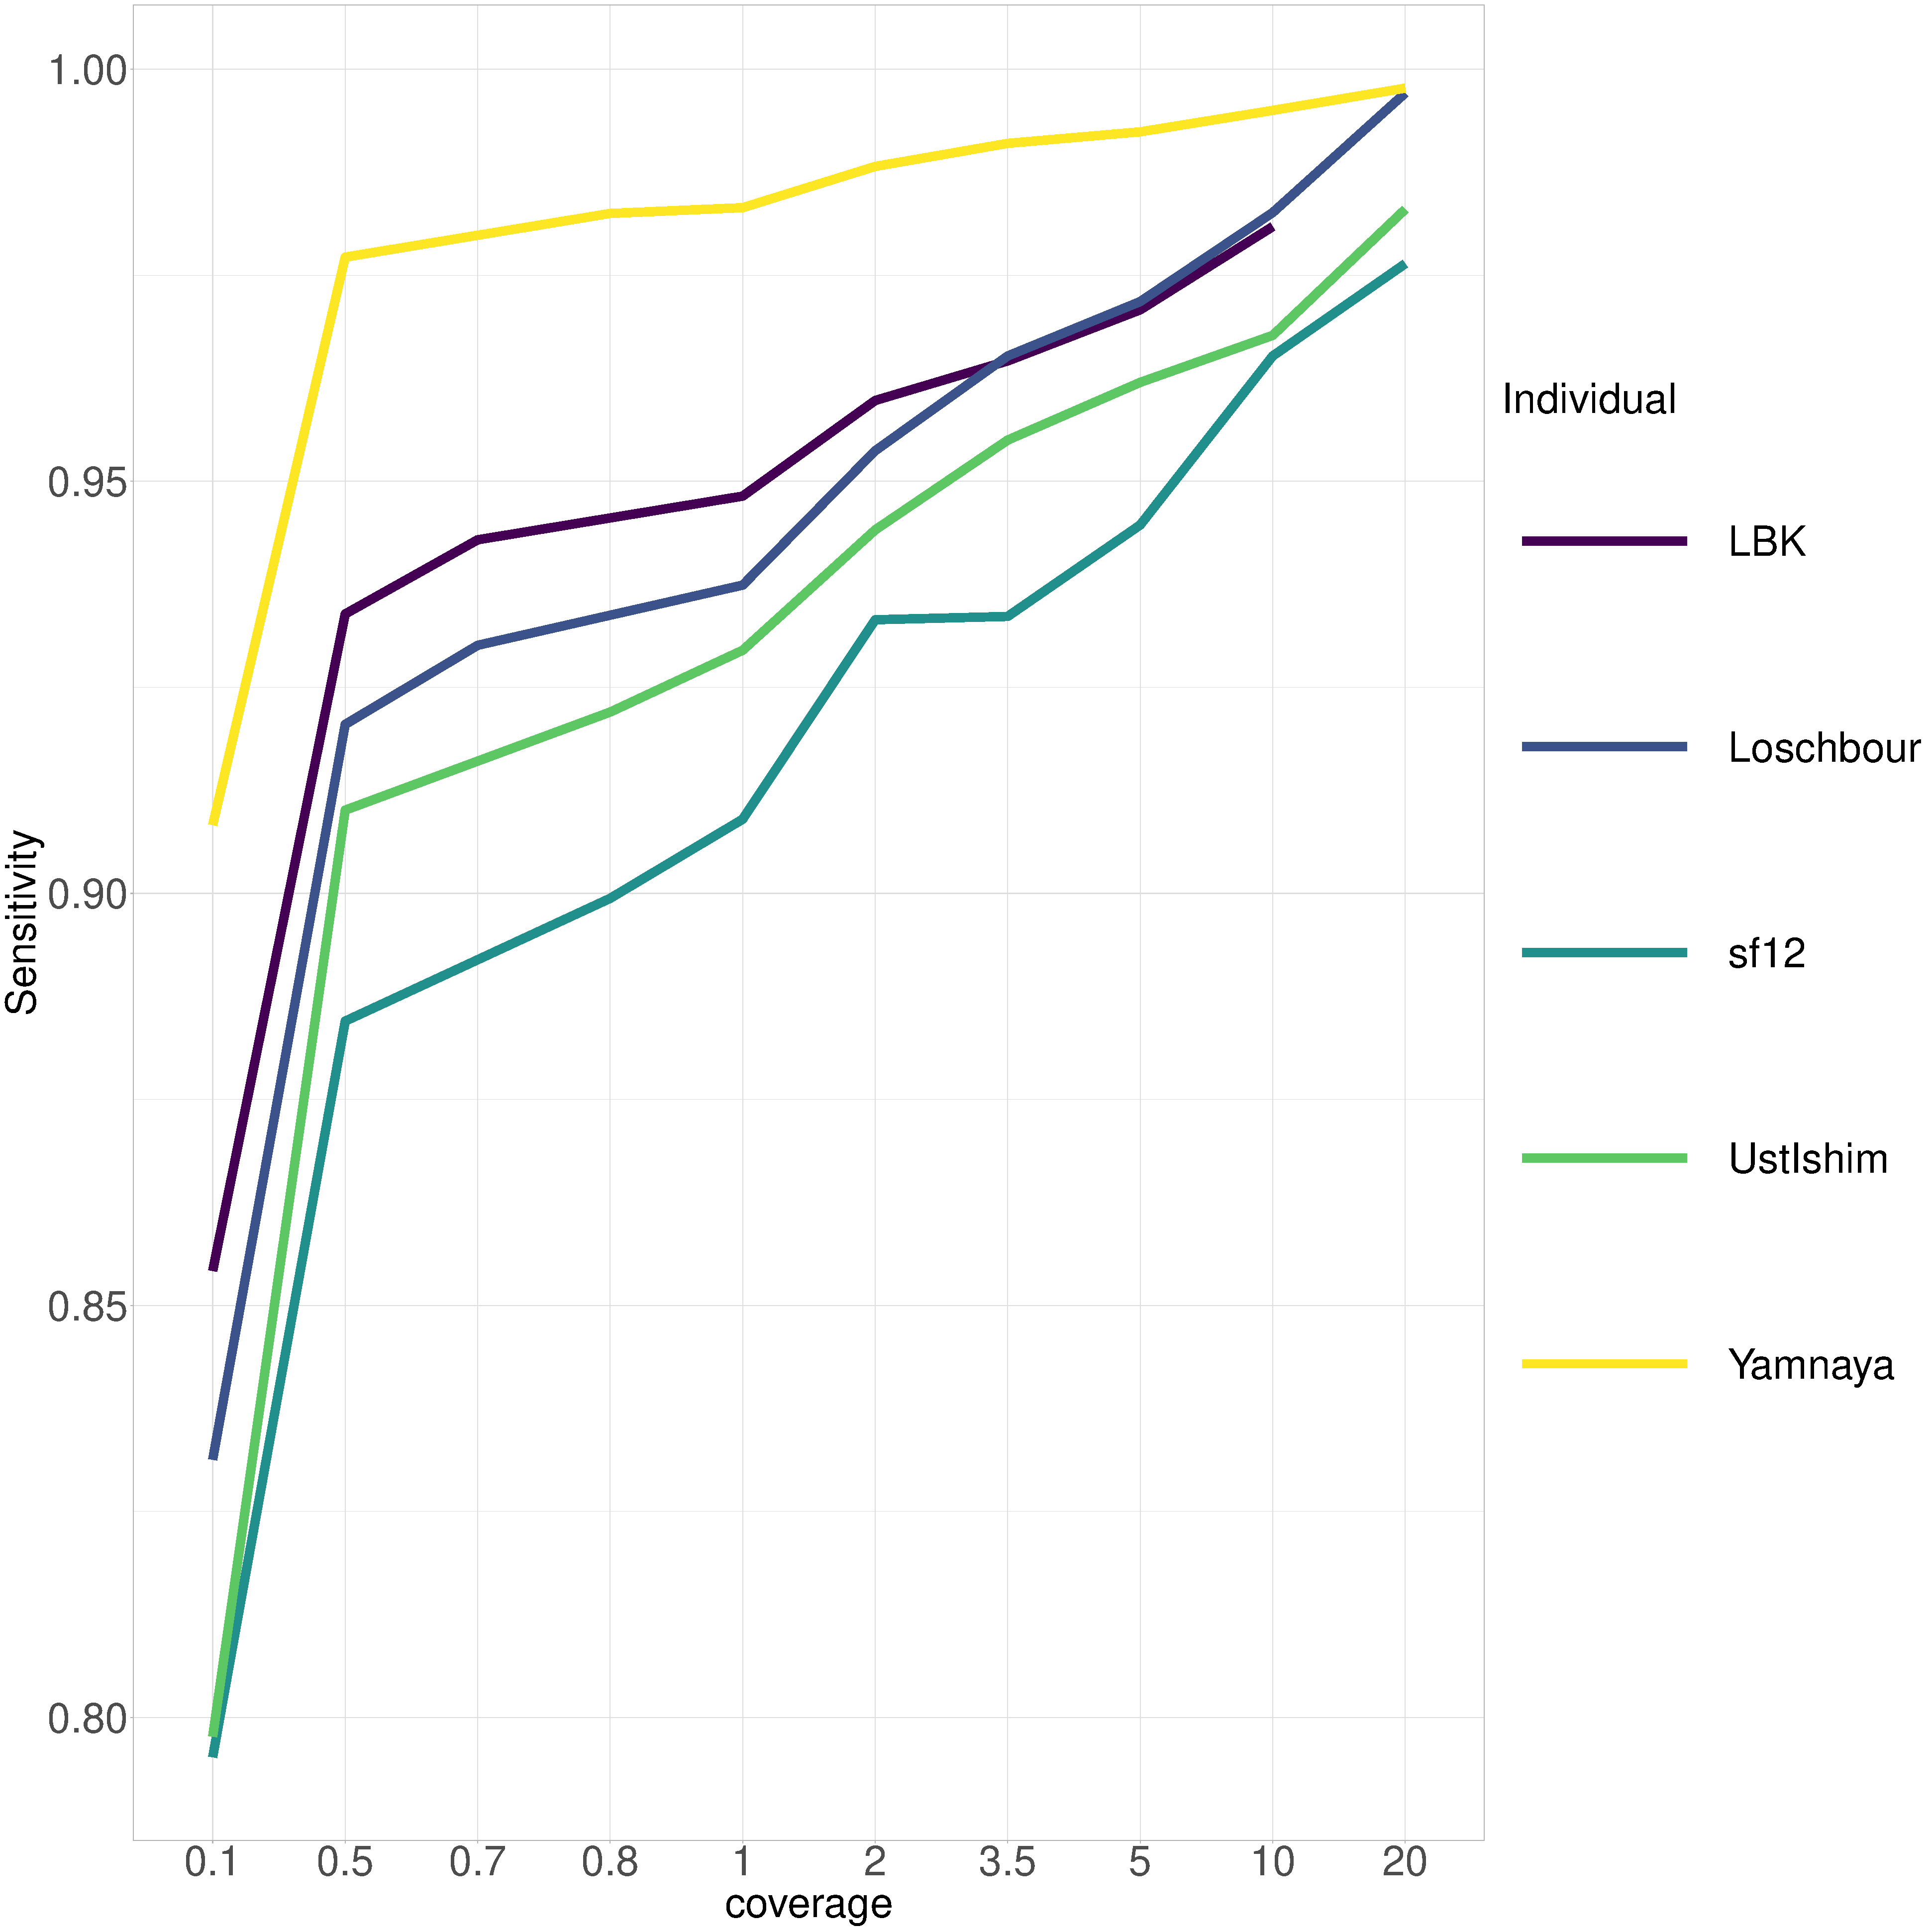
\includegraphics[width=1.0\textwidth]{../images/chapter1/allDownsampled_rtgtools_sensitivity.pdf}
    \caption{Sensitivity of genotype calling at different coverages for different ancient individuals, assuming calls in the full coverage genome are correct,  calculated using rtg-tools.}
    \label{fig:Sensitivity_downsampled_rtgtools}
\end{figure}

\begin{figure}[htp]
    \centering
    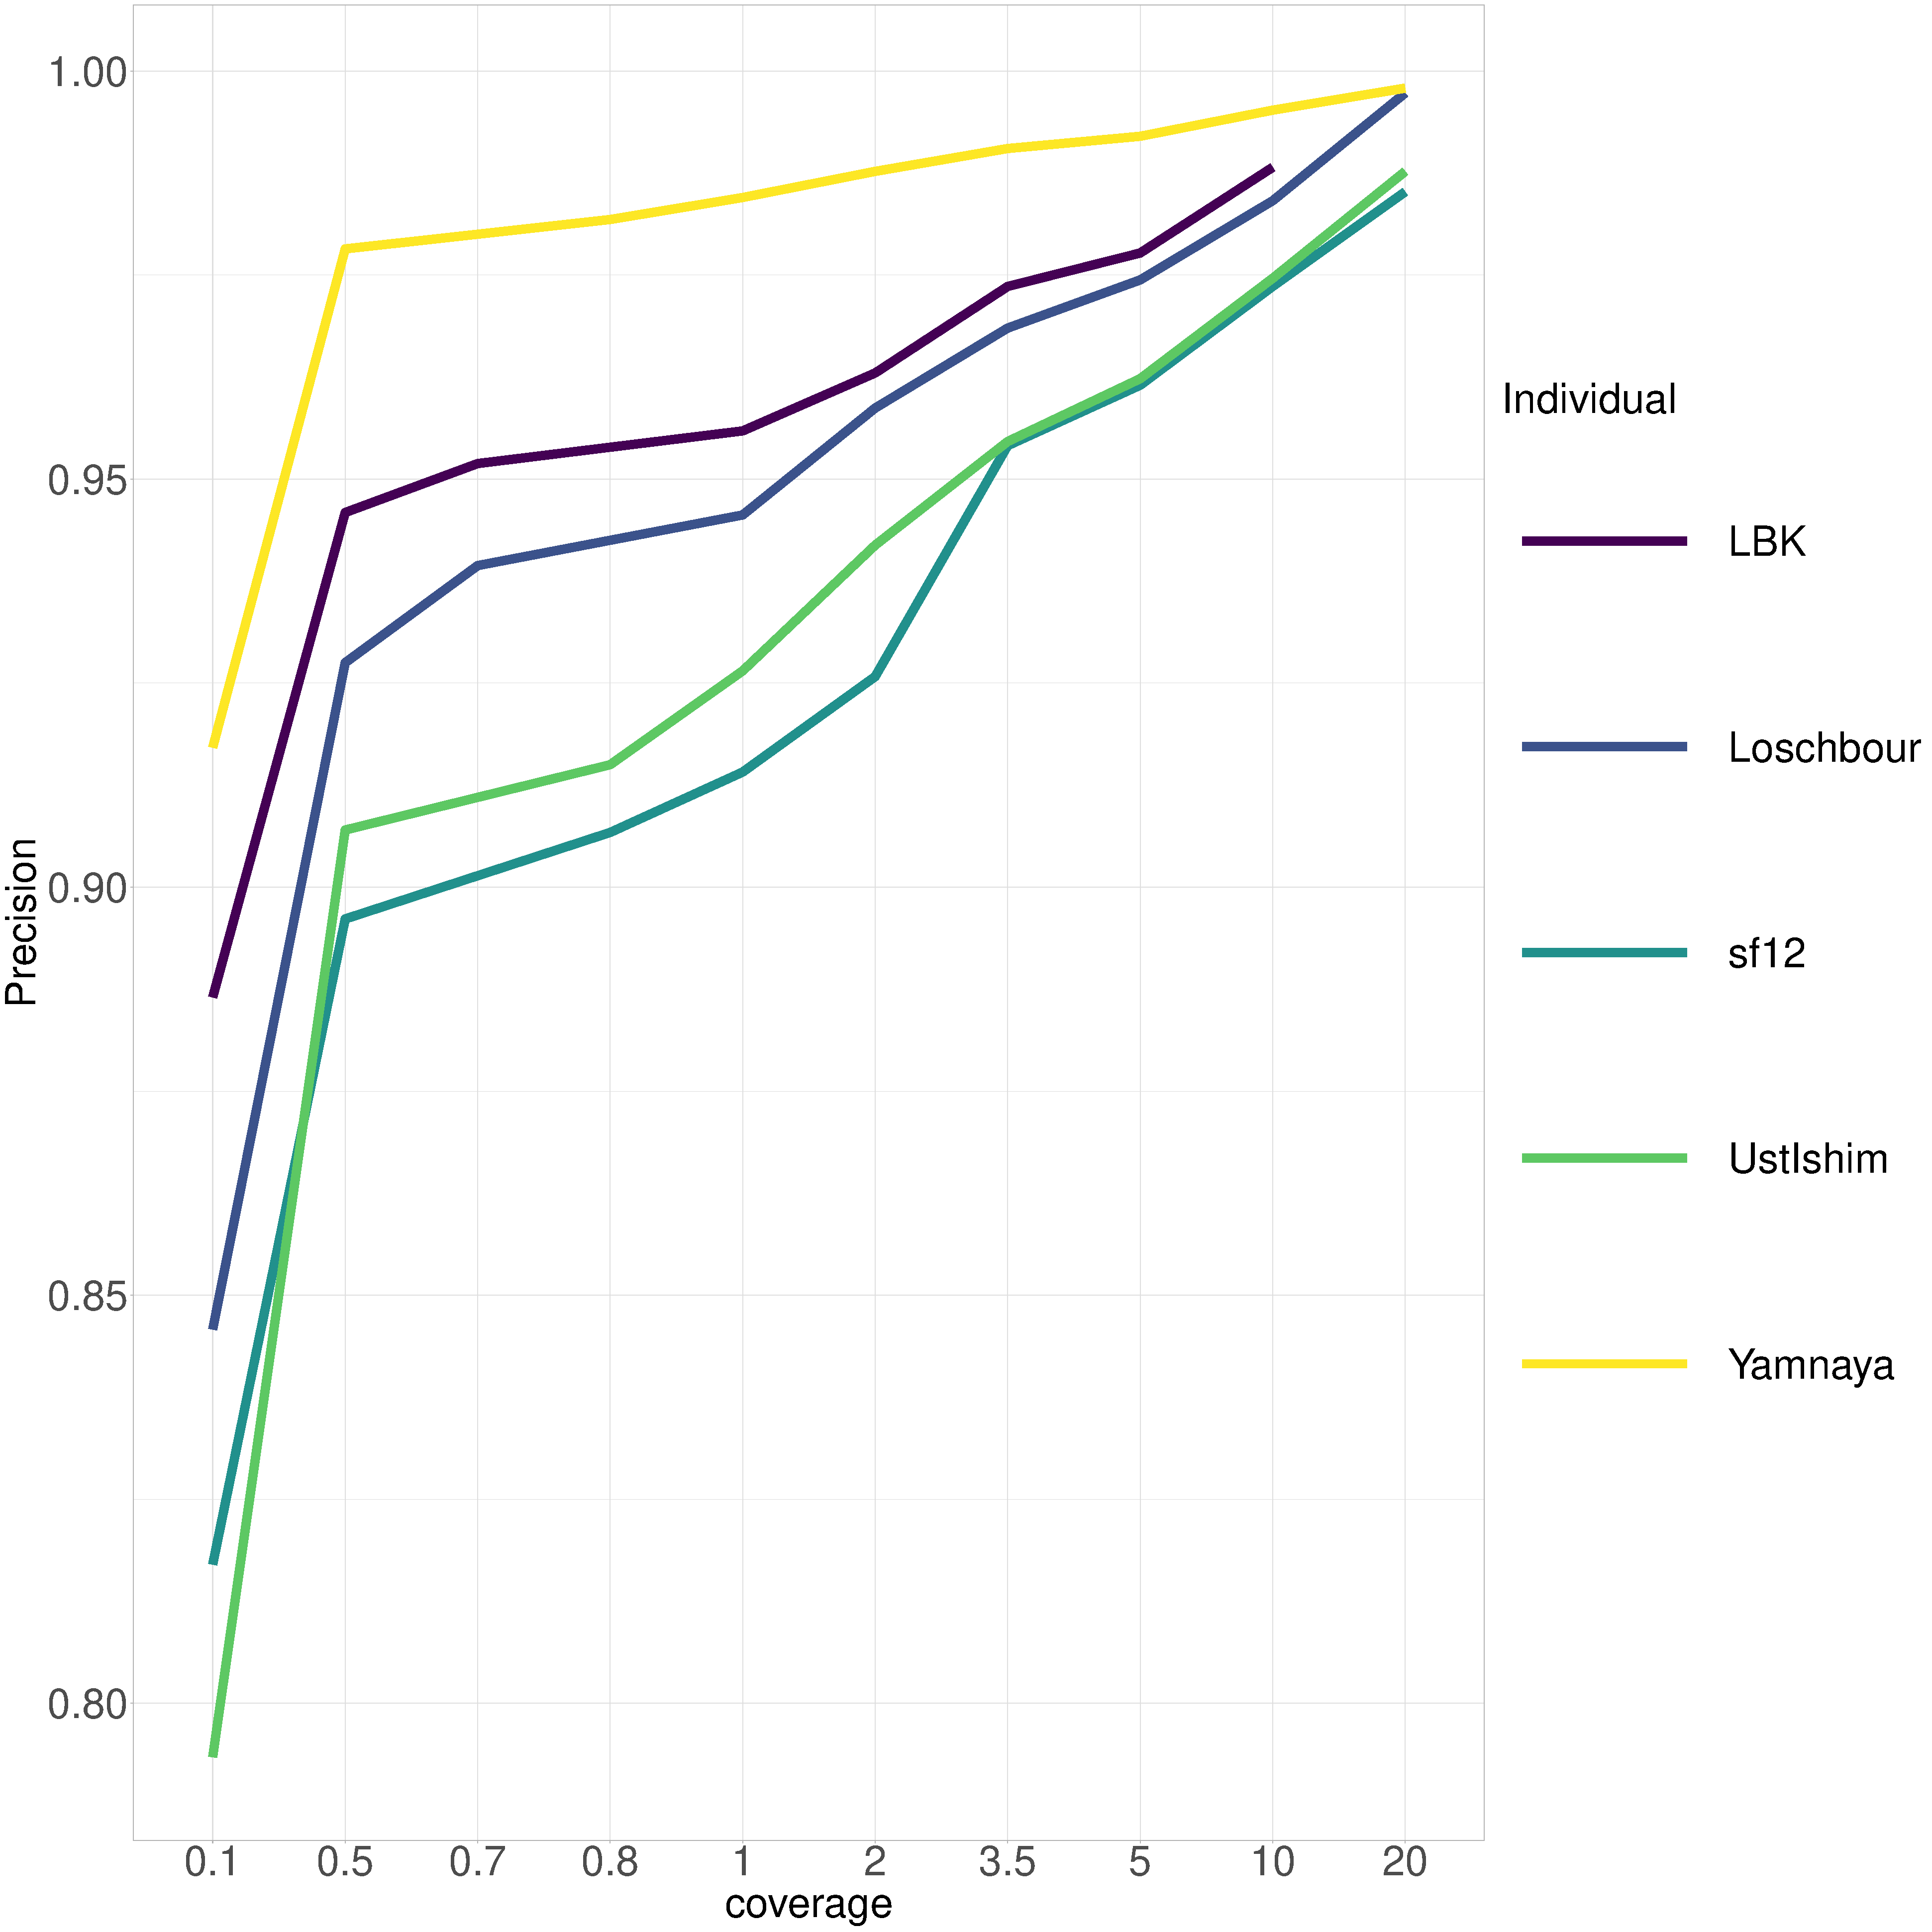
\includegraphics[width=1.0\textwidth]{../images/chapter1/allDownsampled_rtgtools_Precision.pdf}
    \caption{Precision of genotype calling at different coverages for different ancient individuals, assuming calls in the full coverage genome are correct,  calculated using rtg-tools.}
    \label{fig:precision_downsampled_rtgtools}
\end{figure}



\begin{table}
\centering
\begin{tabular}[t]{llllr}
\toprule
stage & total & transitions & transversions & t/v ratio\\
\midrule
atlas & 77,876,460 & 52,693,235 & 25,183,225 & 2.09\\
Post-imputation & 77,815,634 & 52,655,160 & 25,160,474 & 2.09\\
ChromoPainter & 430,088 & 351,087 & 79,000 & 4.44\\
\bottomrule
\end{tabular}
\caption{Number of SNPs retained at different steps of the analysis pipeline. t/v ratio is the ratio of transitions to transversions.}
\end{table}

\begingroup\fontsize{8}{10}\selectfont

\begin{longtable}[t]{lrllllll}
\toprule
Ind & Coverage & Type & total & hom\_ref & hom\_alt & het & missing\\
\midrule
LBK & 0.1 & atlas & 7,863,659 & 7,588,206 & 261,066 & 14,387 & 70,012,596\\
LBK & 0.1 & chromopainter & 174,772 & 82,535 & 35,669 & 56,568 & 255,315\\
LBK & 0.1 & glimpse & 31,789,601 & 30,462,480 & 518,406 & 808,715 & 46,026,033\\
LBK & 0.5 & atlas & 31,594,229 & 30,407,259 & 969,621 & 217,349 & 46,281,316\\
LBK & 0.5 & chromopainter & 396,582 & 183,341 & 82,675 & 130,566 & 33,505\\
LBK & 0.5 & glimpse & 71,596,325 & 68,472,726 & 1,223,743 & 1,899,856 & 6,219,309\\
LBK & 0.7 & atlas & 41,843,708 & 40,197,199 & 1,231,550 & 414,959 & 36,031,516\\
LBK & 0.7 & chromopainter & 420,309 & 193,890 & 88,078 & 138,341 & 9,778\\
LBK & 0.7 & glimpse & 75,872,626 & 72,532,663 & 1,306,213 & 2,033,750 & 1,943,008\\
LBK & 1.0 & atlas & 49,687,572 & 47,648,221 & 1,401,883 & 637,468 & 28,187,240\\
LBK & 1.0 & chromopainter & 427,072 & 196,857 & 89,918 & 140,297 & 3,015\\
LBK & 1.0 & glimpse & 77,152,471 & 73,739,162 & 1,334,040 & 2,079,269 & 663,163\\
LBK & 2.0 & atlas & 66,701,209 & 63,534,792 & 1,619,653 & 1,546,764 & 11,172,575\\
LBK & 2.0 & chromopainter & 430,050 & 197,939 & 91,166 & 140,945 & 37\\
LBK & 2.0 & glimpse & 77,778,825 & 74,307,718 & 1,346,120 & 2,124,987 & 36,809\\
LBK & 3.5 & atlas & 74,554,206 & 70,453,001 & 1,534,742 & 2,566,463 & 3,318,536\\
LBK & 3.5 & chromopainter & 430,087 & 197,854 & 91,454 & 140,779 & 0\\
LBK & 3.5 & glimpse & 77,806,040 & 74,318,824 & 1,339,785 & 2,147,431 & 9,594\\
LBK & 5.0 & atlas & 76,607,872 & 72,092,675 & 1,425,203 & 3,089,994 & 1,264,050\\
LBK & 5.0 & chromopainter & 430,087 & 197,758 & 91,555 & 140,774 & 0\\
LBK & 5.0 & glimpse & 77,810,787 & 74,319,369 & 1,334,420 & 2,156,998 & 4,847\\
LBK & 10.0 & atlas & 77,581,890 & 73,218,587 & 1,303,557 & 3,059,746 & 288,413\\
LBK & 10.0 & chromopainter & 430,087 & 197,767 & 91,671 & 140,649 & 0\\
LBK & 10.0 & glimpse & 77,814,052 & 74,329,568 & 1,323,705 & 2,160,779 & 1,582\\
LBK & 20.0 & atlas & 77,694,833 & 73,820,576 & 1,290,921 & 2,583,336 & 174,119\\
LBK & 20.0 & chromopainter & 430,087 & 197,818 & 91,731 & 140,538 & 0\\
LBK & 20.0 & glimpse & 77,815,338 & 74,343,714 & 1,316,235 & 2,155,389 & 296\\
Loschbour & 0.1 & atlas & 7,628,084 & 7,370,184 & 245,862 & 12,038 & 70,245,058\\
Loschbour & 0.1 & chromopainter & 174,772 & 86,532 & 38,706 & 49,534 & 255,315\\
Loschbour & 0.1 & glimpse & 31,789,601 & 30,519,105 & 565,276 & 705,220 & 46,026,033\\
Loschbour & 0.5 & atlas & 30,780,528 & 29,712,532 & 916,081 & 151,915 & 47,081,605\\
Loschbour & 0.5 & chromopainter & 396,582 & 195,412 & 93,591 & 107,579 & 33,505\\
Loschbour & 0.5 & glimpse & 71,596,325 & 68,667,343 & 1,373,792 & 1,555,190 & 6,219,309\\
Loschbour & 0.7 & atlas & 40,883,211 & 39,425,706 & 1,175,631 & 281,874 & 36,973,485\\
Loschbour & 0.7 & chromopainter & 420,309 & 207,169 & 99,953 & 113,187 & 9,778\\
Loschbour & 0.7 & glimpse & 75,872,626 & 72,748,733 & 1,472,121 & 1,651,772 & 1,943,008\\
Loschbour & 1.0 & atlas & 48,650,549 & 46,860,231 & 1,358,909 & 431,409 & 29,201,103\\
Loschbour & 1.0 & chromopainter & 427,072 & 210,281 & 102,198 & 114,593 & 3,015\\
Loschbour & 1.0 & glimpse & 77,152,471 & 73,963,816 & 1,507,099 & 1,681,556 & 663,163\\
Loschbour & 2.0 & atlas & 65,853,923 & 63,144,388 & 1,658,474 & 1,051,061 & 11,983,909\\
Loschbour & 2.0 & chromopainter & 430,050 & 211,678 & 104,100 & 114,272 & 37\\
Loschbour & 2.0 & glimpse & 77,778,825 & 74,544,266 & 1,527,789 & 1,706,770 & 36,809\\
Loschbour & 3.5 & atlas & 74,181,557 & 70,747,172 & 1,658,730 & 1,775,655 & 3,645,307\\
Loschbour & 3.5 & chromopainter & 430,087 & 211,655 & 104,673 & 113,759 & 0\\
Loschbour & 3.5 & glimpse & 77,806,040 & 74,562,077 & 1,524,547 & 1,719,416 & 9,594\\
Loschbour & 5.0 & atlas & 76,517,579 & 72,731,738 & 1,588,393 & 2,197,448 & 1,304,225\\
Loschbour & 5.0 & chromopainter & 430,087 & 211,636 & 104,949 & 113,502 & 0\\
Loschbour & 5.0 & glimpse & 77,810,787 & 74,564,499 & 1,518,703 & 1,727,585 & 4,847\\
Loschbour & 10.0 & atlas & 77,674,711 & 73,807,087 & 1,481,465 & 2,386,159 & 142,717\\
Loschbour & 10.0 & chromopainter & 430,087 & 211,630 & 105,182 & 113,275 & 0\\
Loschbour & 10.0 & glimpse & 77,814,052 & 74,563,530 & 1,508,188 & 1,742,334 & 1,582\\
Loschbour & 20.0 & atlas & 77,768,448 & 74,340,455 & 1,469,135 & 1,958,858 & 48,221\\
Loschbour & 20.0 & chromopainter & 430,087 & 211,706 & 105,332 & 113,049 & 0\\
Loschbour & 20.0 & glimpse & 77,815,338 & 74,581,352 & 1,497,789 & 1,736,197 & 296\\
sf12 & 0.1 & atlas & 7,587,373 & 7,336,322 & 236,147 & 14,904 & 70,288,793\\
sf12 & 0.1 & chromopainter & 174,772 & 84,128 & 34,002 & 56,642 & 255,315\\
sf12 & 0.1 & glimpse & 31,789,601 & 30,484,260 & 487,734 & 817,607 & 46,026,033\\
sf12 & 0.5 & atlas & 30,688,125 & 29,606,869 & 898,622 & 182,634 & 47,186,835\\
sf12 & 0.5 & chromopainter & 396,582 & 189,406 & 81,260 & 125,916 & 33,505\\
sf12 & 0.5 & glimpse & 71,596,325 & 68,564,219 & 1,166,608 & 1,865,498 & 6,219,309\\
sf12 & 0.8 & atlas & 40,808,399 & 39,317,115 & 1,151,362 & 339,922 & 37,065,944\\
sf12 & 0.8 & chromopainter & 420,309 & 200,429 & 87,984 & 131,896 & 9,778\\
sf12 & 0.8 & glimpse & 75,872,626 & 72,625,472 & 1,257,618 & 1,989,536 & 1,943,008\\
sf12 & 1.0 & atlas & 48,588,367 & 46,748,059 & 1,324,815 & 515,493 & 29,285,496\\
sf12 & 1.0 & chromopainter & 427,072 & 203,684 & 90,629 & 132,759 & 3,015\\
sf12 & 1.0 & glimpse & 77,152,471 & 73,829,354 & 1,293,711 & 2,029,406 & 663,163\\
sf12 & 2.0 & atlas & 65,862,294 & 63,043,247 & 1,581,552 & 1,237,495 & 12,009,874\\
sf12 & 2.0 & chromopainter & 430,050 & 204,670 & 93,985 & 131,395 & 37\\
sf12 & 2.0 & glimpse & 77,778,825 & 74,373,518 & 1,323,114 & 2,082,193 & 36,809\\
sf12 & 3.5 & atlas & 74,228,518 & 70,594,011 & 1,544,188 & 2,090,319 & 3,642,111\\
sf12 & 3.5 & chromopainter & 430,087 & 204,353 & 95,572 & 130,162 & 0\\
sf12 & 3.5 & glimpse & 77,806,040 & 74,350,373 & 1,325,545 & 2,130,122 & 9,594\\
sf12 & 5.0 & atlas & 76,539,118 & 72,461,162 & 1,449,890 & 2,628,066 & 1,330,339\\
sf12 & 5.0 & chromopainter & 430,087 & 204,286 & 96,166 & 129,635 & 0\\
sf12 & 5.0 & glimpse & 77,810,787 & 74,331,202 & 1,321,586 & 2,157,999 & 4,847\\
sf12 & 10.0 & atlas & 77,660,653 & 73,356,950 & 1,308,470 & 2,995,233 & 206,644\\
sf12 & 10.0 & chromopainter & 430,087 & 204,392 & 97,098 & 128,597 & 0\\
sf12 & 10.0 & glimpse & 77,814,052 & 74,368,059 & 1,317,620 & 2,128,373 & 1,582\\
sf12 & 20.0 & atlas & 77,758,773 & 73,930,624 & 1,278,517 & 2,549,632 & 106,192\\
sf12 & 20.0 & chromopainter & 430,087 & 204,693 & 97,630 & 127,764 & 0\\
sf12 & 20.0 & glimpse & 77,815,338 & 74,415,488 & 1,310,559 & 2,089,291 & 296\\
UstIshim & 0.1 & atlas & 7,786,181 & 7,432,667 & 329,609 & 23,905 & 70,086,937\\
UstIshim & 0.1 & chromopainter & 174,772 & 80,029 & 33,344 & 61,399 & 255,315\\
UstIshim & 0.1 & glimpse & 31,789,601 & 30,347,768 & 482,910 & 958,923 & 46,026,033\\
UstIshim & 0.5 & atlas & 31,488,887 & 30,337,316 & 958,513 & 193,058 & 46,372,621\\
UstIshim & 0.5 & chromopainter & 396,582 & 180,030 & 81,103 & 135,449 & 33,505\\
UstIshim & 0.5 & glimpse & 71,596,325 & 68,324,000 & 1,182,070 & 2,090,255 & 6,219,309\\
UstIshim & 0.8 & atlas & 41,850,784 & 40,269,671 & 1,218,249 & 362,864 & 36,004,942\\
UstIshim & 0.8 & chromopainter & 420,309 & 190,363 & 86,981 & 142,965 & 9,778\\
UstIshim & 0.8 & glimpse & 75,872,626 & 72,373,517 & 1,270,046 & 2,229,063 & 1,943,008\\
UstIshim & 1.0 & atlas & 49,768,765 & 47,831,665 & 1,388,385 & 548,715 & 28,081,614\\
UstIshim & 1.0 & chromopainter & 427,072 & 193,316 & 89,121 & 144,635 & 3,015\\
UstIshim & 1.0 & glimpse & 77,152,471 & 73,597,414 & 1,303,425 & 2,251,632 & 663,163\\
UstIshim & 2.0 & atlas & 67,062,432 & 64,120,181 & 1,614,975 & 1,327,276 & 10,773,728\\
UstIshim & 2.0 & chromopainter & 430,050 & 194,399 & 91,175 & 144,476 & 37\\
UstIshim & 2.0 & glimpse & 77,778,825 & 74,181,418 & 1,322,097 & 2,275,310 & 36,809\\
UstIshim & 3.5 & atlas & 74,919,994 & 71,129,843 & 1,524,122 & 2,266,029 & 2,905,623\\
UstIshim & 3.5 & chromopainter & 430,087 & 194,227 & 91,973 & 143,887 & 0\\
UstIshim & 3.5 & glimpse & 77,806,040 & 74,206,978 & 1,316,655 & 2,282,407 & 9,594\\
UstIshim & 5.0 & atlas & 76,888,994 & 72,621,237 & 1,403,149 & 2,864,608 & 931,764\\
UstIshim & 5.0 & chromopainter & 430,087 & 194,165 & 92,403 & 143,519 & 0\\
UstIshim & 5.0 & glimpse & 77,810,787 & 74,211,695 & 1,308,177 & 2,290,915 & 4,847\\
UstIshim & 10.0 & atlas & 77,723,502 & 73,311,539 & 1,260,452 & 3,151,511 & 93,822\\
UstIshim & 10.0 & chromopainter & 430,087 & 194,059 & 92,805 & 143,223 & 0\\
UstIshim & 10.0 & glimpse & 77,814,052 & 74,198,170 & 1,291,089 & 2,324,793 & 1,582\\
UstIshim & 20.0 & atlas & 77,782,585 & 73,919,501 & 1,244,171 & 2,618,913 & 34,154\\
UstIshim & 20.0 & chromopainter & 430,087 & 194,223 & 93,081 & 142,783 & 0\\
UstIshim & 20.0 & glimpse & 77,815,338 & 74,244,692 & 1,275,230 & 2,295,416 & 296\\
Yamnaya & 0.1 & atlas & 8,165,424 & 7,837,096 & 310,333 & 17,995 & 69,707,971\\
Yamnaya & 0.1 & chromopainter & 174,772 & 82,050 & 36,011 & 56,711 & 255,315\\
Yamnaya & 0.1 & glimpse & 31,789,601 & 30,437,553 & 540,479 & 811,569 & 46,026,033\\
Yamnaya & 0.5 & atlas & 32,588,629 & 31,348,275 & 1,007,256 & 233,098 & 45,273,342\\
Yamnaya & 0.5 & chromopainter & 396,582 & 183,027 & 83,207 & 130,348 & 33,505\\
Yamnaya & 0.5 & glimpse & 71,596,325 & 68,452,137 & 1,270,312 & 1,873,876 & 6,219,309\\
Yamnaya & 0.8 & atlas & 42,932,013 & 41,218,304 & 1,265,634 & 448,075 & 34,924,034\\
Yamnaya & 0.8 & chromopainter & 420,309 & 193,465 & 88,637 & 138,207 & 9,778\\
Yamnaya & 0.8 & glimpse & 75,872,626 & 72,514,711 & 1,359,849 & 1,998,066 & 1,943,008\\
Yamnaya & 1.0 & atlas & 50,685,590 & 48,564,638 & 1,428,476 & 692,476 & 27,165,519\\
Yamnaya & 1.0 & chromopainter & 427,072 & 196,530 & 90,041 & 140,501 & 3,015\\
Yamnaya & 1.0 & glimpse & 77,152,471 & 73,722,704 & 1,389,219 & 2,040,548 & 663,163\\
Yamnaya & 2.0 & atlas & 66,872,411 & 63,571,601 & 1,622,362 & 1,678,448 & 10,964,758\\
Yamnaya & 2.0 & chromopainter & 430,050 & 197,631 & 90,666 & 141,753 & 37\\
Yamnaya & 2.0 & glimpse & 77,778,825 & 74,301,224 & 1,409,000 & 2,068,601 & 36,809\\
Yamnaya & 3.5 & atlas & 73,859,932 & 69,713,521 & 1,532,552 & 2,613,859 & 3,966,618\\
Yamnaya & 3.5 & chromopainter & 430,087 & 197,605 & 90,706 & 141,776 & 0\\
Yamnaya & 3.5 & glimpse & 77,806,040 & 74,324,453 & 1,410,929 & 2,070,658 & 9,594\\
Yamnaya & 5.0 & atlas & 75,688,825 & 71,333,069 & 1,446,906 & 2,908,850 & 2,133,156\\
Yamnaya & 5.0 & chromopainter & 430,087 & 197,508 & 90,698 & 141,881 & 0\\
Yamnaya & 5.0 & glimpse & 77,810,787 & 74,327,884 & 1,410,512 & 2,072,391 & 4,847\\
Yamnaya & 10.0 & atlas & 76,836,943 & 72,953,272 & 1,372,488 & 2,511,183 & 981,054\\
Yamnaya & 10.0 & chromopainter & 430,087 & 197,539 & 90,708 & 141,840 & 0\\
Yamnaya & 10.0 & glimpse & 77,814,052 & 74,334,567 & 1,409,677 & 2,069,808 & 1,582\\
Yamnaya & 20.0 & atlas & 77,210,145 & 73,701,551 & 1,373,349 & 2,135,245 & 606,580\\
Yamnaya & 20.0 & chromopainter & 430,087 & 197,565 & 90,739 & 141,783 & 0\\
Yamnaya & 20.0 & glimpse & 77,815,338 & 74,343,330 & 1,409,070 & 2,062,938 & 296\\
\bottomrule
\caption{Number and type of variants passing different steps of the analysis pipeline for different downsamples at different coverages. `atlas' refers to after variant calling with atlas, `glimpse` to after imputation with GLIMPSE and `chromopainter' to ChromoPainter analysis.}\\
\end{longtable}
\endgroup{}


As expected, both the overall sensitivity and precision of imputation fell with coverage, with a particularly sharp drop-off in both metrics between 0.5x and 0.1x coverage. Whilst I did not investigate this, other studies have shown the probability of any one SNP in an sample being correctly imputed depends strongly on the frequency in the reference panel \cite{hui2020evaluating, rubinacci2021efficient}. In particular, alleles which are rare in the reference panel are less likely to be imputed correctly.

Different downsampled individuals varied in the precision and sensitivity of genotype imputation. At all coverages, Yamnaya had the both the highest sensitivity and precision. This may be because the imputation reference panel contains a high proportion of present-day Europeans, who have a relatively higher proportion of recent Yamnaya-like ancestry relative to e.g. Hunter Gatherer-like ancestry \cite{Haak2005}. Many studies in present-day individuals have shown that imputation accuracy increases when more haplotypes which are close to the target individual are found in the reference panel \cite{HUANG2009235, delaneau2018integrative}. On the other hand, the sample Ust'Ishim is known to have contributed very little genetic ancestry to present-day populations \cite{Prufer2014} and may therefore have fewer closely matching haplotypes in the reference panel, and a correspondingly lower imputation accuracy. 

Imputation accuracy may also be related to demographic history. Populations which are known to have smaller effective population size, such as Western-Hunter Gathers, also contain longer tracts between individuals which are identical by descent (IBD) \cite{browning2015accurate} and fewer heterozygous positions. As imputation relies on matching IBD tracts between individuals, imputation accuracy increases where individuals share more IBD \cite{kong2008detection}. However, this would not be the case in this analysis as there are not hunter-gatherers in the reference panel for target hunter-gatherers to share IBD with. Additionally, switch-errors during the pre-phasing step of imputation may harm imputation accuracy, so a reduced density of heterozygous positions may result in increased accuracy. 

\begingroup\fontsize{8}{10}\selectfont

\begin{longtable}[t]{lllrr}
\toprule
Ind & Coverage & Type & Precision & Sensitivity\\
\midrule
\endfirsthead
\multicolumn{5}{@{}l}{\textit{(continued)}}\\
\toprule
Ind & Coverage & Type & Precision & Sensitivity\\
\midrule
\endhead

\endfoot
\bottomrule
\endlastfoot
LBK & 0.1 & heterozygous & 0.9687 & 0.4315\\
LBK & 0.1 & homozygous & 0.9957 & 0.9074\\
LBK & 0.5 & heterozygous & 0.9759 & 0.4688\\
LBK & 0.5 & homozygous & 0.9974 & 0.9659\\
LBK & 0.7 & heterozygous & 0.9764 & 0.4736\\
LBK & 0.7 & homozygous & 0.9981 & 0.9721\\
LBK & 1 & heterozygous & 0.9763 & 0.4760\\
LBK & 1 & homozygous & 0.9985 & 0.9754\\
LBK & 10 & heterozygous & 0.9866 & 0.4919\\
LBK & 10 & homozygous & 1.0000 & 0.9924\\
LBK & 2 & heterozygous & 0.9789 & 0.4813\\
LBK & 2 & homozygous & 0.9995 & 0.9819\\
LBK & 3.5 & heterozygous & 0.9813 & 0.4852\\
LBK & 3.5 & homozygous & 0.9999 & 0.9863\\
LBK & 5 & heterozygous & 0.9838 & 0.4875\\
LBK & 5 & homozygous & 1.0000 & 0.9887\\
Loschbour & 0.1 & heterozygous & 0.9541 & 0.4420\\
Loschbour & 0.1 & homozygous & 0.9962 & 0.9142\\
Loschbour & 0.5 & heterozygous & 0.9759 & 0.4730\\
Loschbour & 0.5 & homozygous & 0.9979 & 0.9627\\
Loschbour & 0.7 & heterozygous & 0.9773 & 0.4769\\
Loschbour & 0.7 & homozygous & 0.9984 & 0.9688\\
Loschbour & 1 & heterozygous & 0.9791 & 0.4794\\
Loschbour & 1 & homozygous & 0.9988 & 0.9721\\
Loschbour & 10 & heterozygous & 0.9885 & 0.4946\\
Loschbour & 10 & homozygous & 1.0000 & 0.9915\\
Loschbour & 2 & heterozygous & 0.9826 & 0.4842\\
Loschbour & 2 & homozygous & 0.9996 & 0.9795\\
Loschbour & 20 & heterozygous & 0.9995 & 0.4988\\
Loschbour & 20 & homozygous & 1.0000 & 0.9947\\
Loschbour & 3.5 & heterozygous & 0.9850 & 0.4883\\
Loschbour & 3.5 & homozygous & 0.9999 & 0.9843\\
Loschbour & 5 & heterozygous & 0.9884 & 0.4906\\
Loschbour & 5 & homozygous & 1.0000 & 0.9873\\
sf12 & 0.1 & heterozygous & 0.9606 & 0.4356\\
sf12 & 0.1 & homozygous & 0.9973 & 0.9011\\
sf12 & 0.5 & heterozygous & 0.9795 & 0.4713\\
sf12 & 0.5 & homozygous & 0.9989 & 0.9444\\
sf12 & 0.8 & heterozygous & 0.9788 & 0.4752\\
sf12 & 0.8 & homozygous & 0.9992 & 0.9521\\
sf12 & 1 & heterozygous & 0.9775 & 0.4772\\
sf12 & 1 & homozygous & 0.9993 & 0.9570\\
sf12 & 10 & heterozygous & 0.9693 & 0.4915\\
sf12 & 10 & homozygous & 1.0000 & 0.9877\\
sf12 & 2 & heterozygous & 0.9688 & 0.4823\\
sf12 & 2 & homozygous & 0.9997 & 0.9695\\
sf12 & 20 & heterozygous & 0.9798 & 0.4932\\
sf12 & 20 & homozygous & 1.0000 & 0.9936\\
sf12 & 3.5 & heterozygous & 0.9577 & 0.4861\\
sf12 & 3.5 & homozygous & 0.9998 & 0.9785\\
sf12 & 5 & heterozygous & 0.9547 & 0.4880\\
sf12 & 5 & homozygous & 0.9999 & 0.9831\\
UstIshim & 0.1 & heterozygous & 0.9267 & 0.4308\\
UstIshim & 0.1 & homozygous & 0.9935 & 0.8879\\
UstIshim & 0.5 & heterozygous & 0.9650 & 0.4750\\
UstIshim & 0.5 & homozygous & 0.9964 & 0.9505\\
UstIshim & 0.8 & heterozygous & 0.9655 & 0.4794\\
UstIshim & 0.8 & homozygous & 0.9970 & 0.9589\\
UstIshim & 1 & heterozygous & 0.9686 & 0.4817\\
UstIshim & 1 & homozygous & 0.9977 & 0.9634\\
UstIshim & 10 & heterozygous & 0.9733 & 0.4933\\
UstIshim & 10 & homozygous & 1.0000 & 0.9891\\
UstIshim & 2 & heterozygous & 0.9719 & 0.4861\\
UstIshim & 2 & homozygous & 0.9990 & 0.9731\\
UstIshim & 20 & heterozygous & 0.9859 & 0.4960\\
UstIshim & 20 & homozygous & 1.0000 & 0.9935\\
UstIshim & 3.5 & heterozygous & 0.9774 & 0.4888\\
UstIshim & 3.5 & homozygous & 0.9996 & 0.9792\\
UstIshim & 5 & heterozygous & 0.9802 & 0.4906\\
UstIshim & 5 & homozygous & 0.9999 & 0.9831\\
Yamnaya & 0.1 & heterozygous & 0.9662 & 0.4471\\
Yamnaya & 0.1 & homozygous & 0.9990 & 0.9358\\
Yamnaya & 0.5 & heterozygous & 0.9785 & 0.4830\\
Yamnaya & 0.5 & homozygous & 0.9994 & 0.9857\\
Yamnaya & 0.8 & heterozygous & 0.9803 & 0.4868\\
Yamnaya & 0.8 & homozygous & 0.9995 & 0.9896\\
Yamnaya & 1 & heterozygous & 0.9792 & 0.4886\\
Yamnaya & 1 & homozygous & 0.9996 & 0.9912\\
Yamnaya & 10 & heterozygous & 0.9935 & 0.5097\\
Yamnaya & 10 & homozygous & 1.0000 & 0.9974\\
Yamnaya & 2 & heterozygous & 0.9781 & 0.4923\\
Yamnaya & 2 & homozygous & 0.9998 & 0.9939\\
Yamnaya & 20 & heterozygous & 0.9976 & 0.5356\\
Yamnaya & 20 & homozygous & 1.0000 & 0.9981\\
Yamnaya & 3.5 & heterozygous & 0.9829 & 0.4969\\
Yamnaya & 3.5 & homozygous & 0.9999 & 0.9956\\
Yamnaya & 5 & heterozygous & 0.9851 & 0.5027\\
Yamnaya & 5 & homozygous & 0.9999 & 0.9963\\*
\caption{Sensitivity and precision of imputed genotypes stratified by sample, coverage and variant type.}
\end{longtable}
\endgroup{}



\subsection{Phasing accuracy}

I also used rtg-tools to calculate the number of phased heterozygous genotypes where the downsampled individual has the same phase as the full coverage individual (Fig \ref{fig:phasing_performance_downsampled}). I note that this should not be considered to be the same as estimating the switch error rate, since we do not know that the phasing in the full-coverage individual is the true phase. However, this can be used as a rough proxy for switch errors, since it is known that phasing in lower coverage individuals is likely to be less accurate than those in the high coverage individuals \cite{rubinacci2021efficient}.

Phase agreement with the full-coverage sample increased with increasing coverage. Such results are difficult to interpret because each sample has a different level of heterozygosity. However, given switch errors occur on a scale greater than the estimated chunk size, they are not expected to significantly contribute towards painting accuracy.

\begin{figure}[htp]
    \centering
    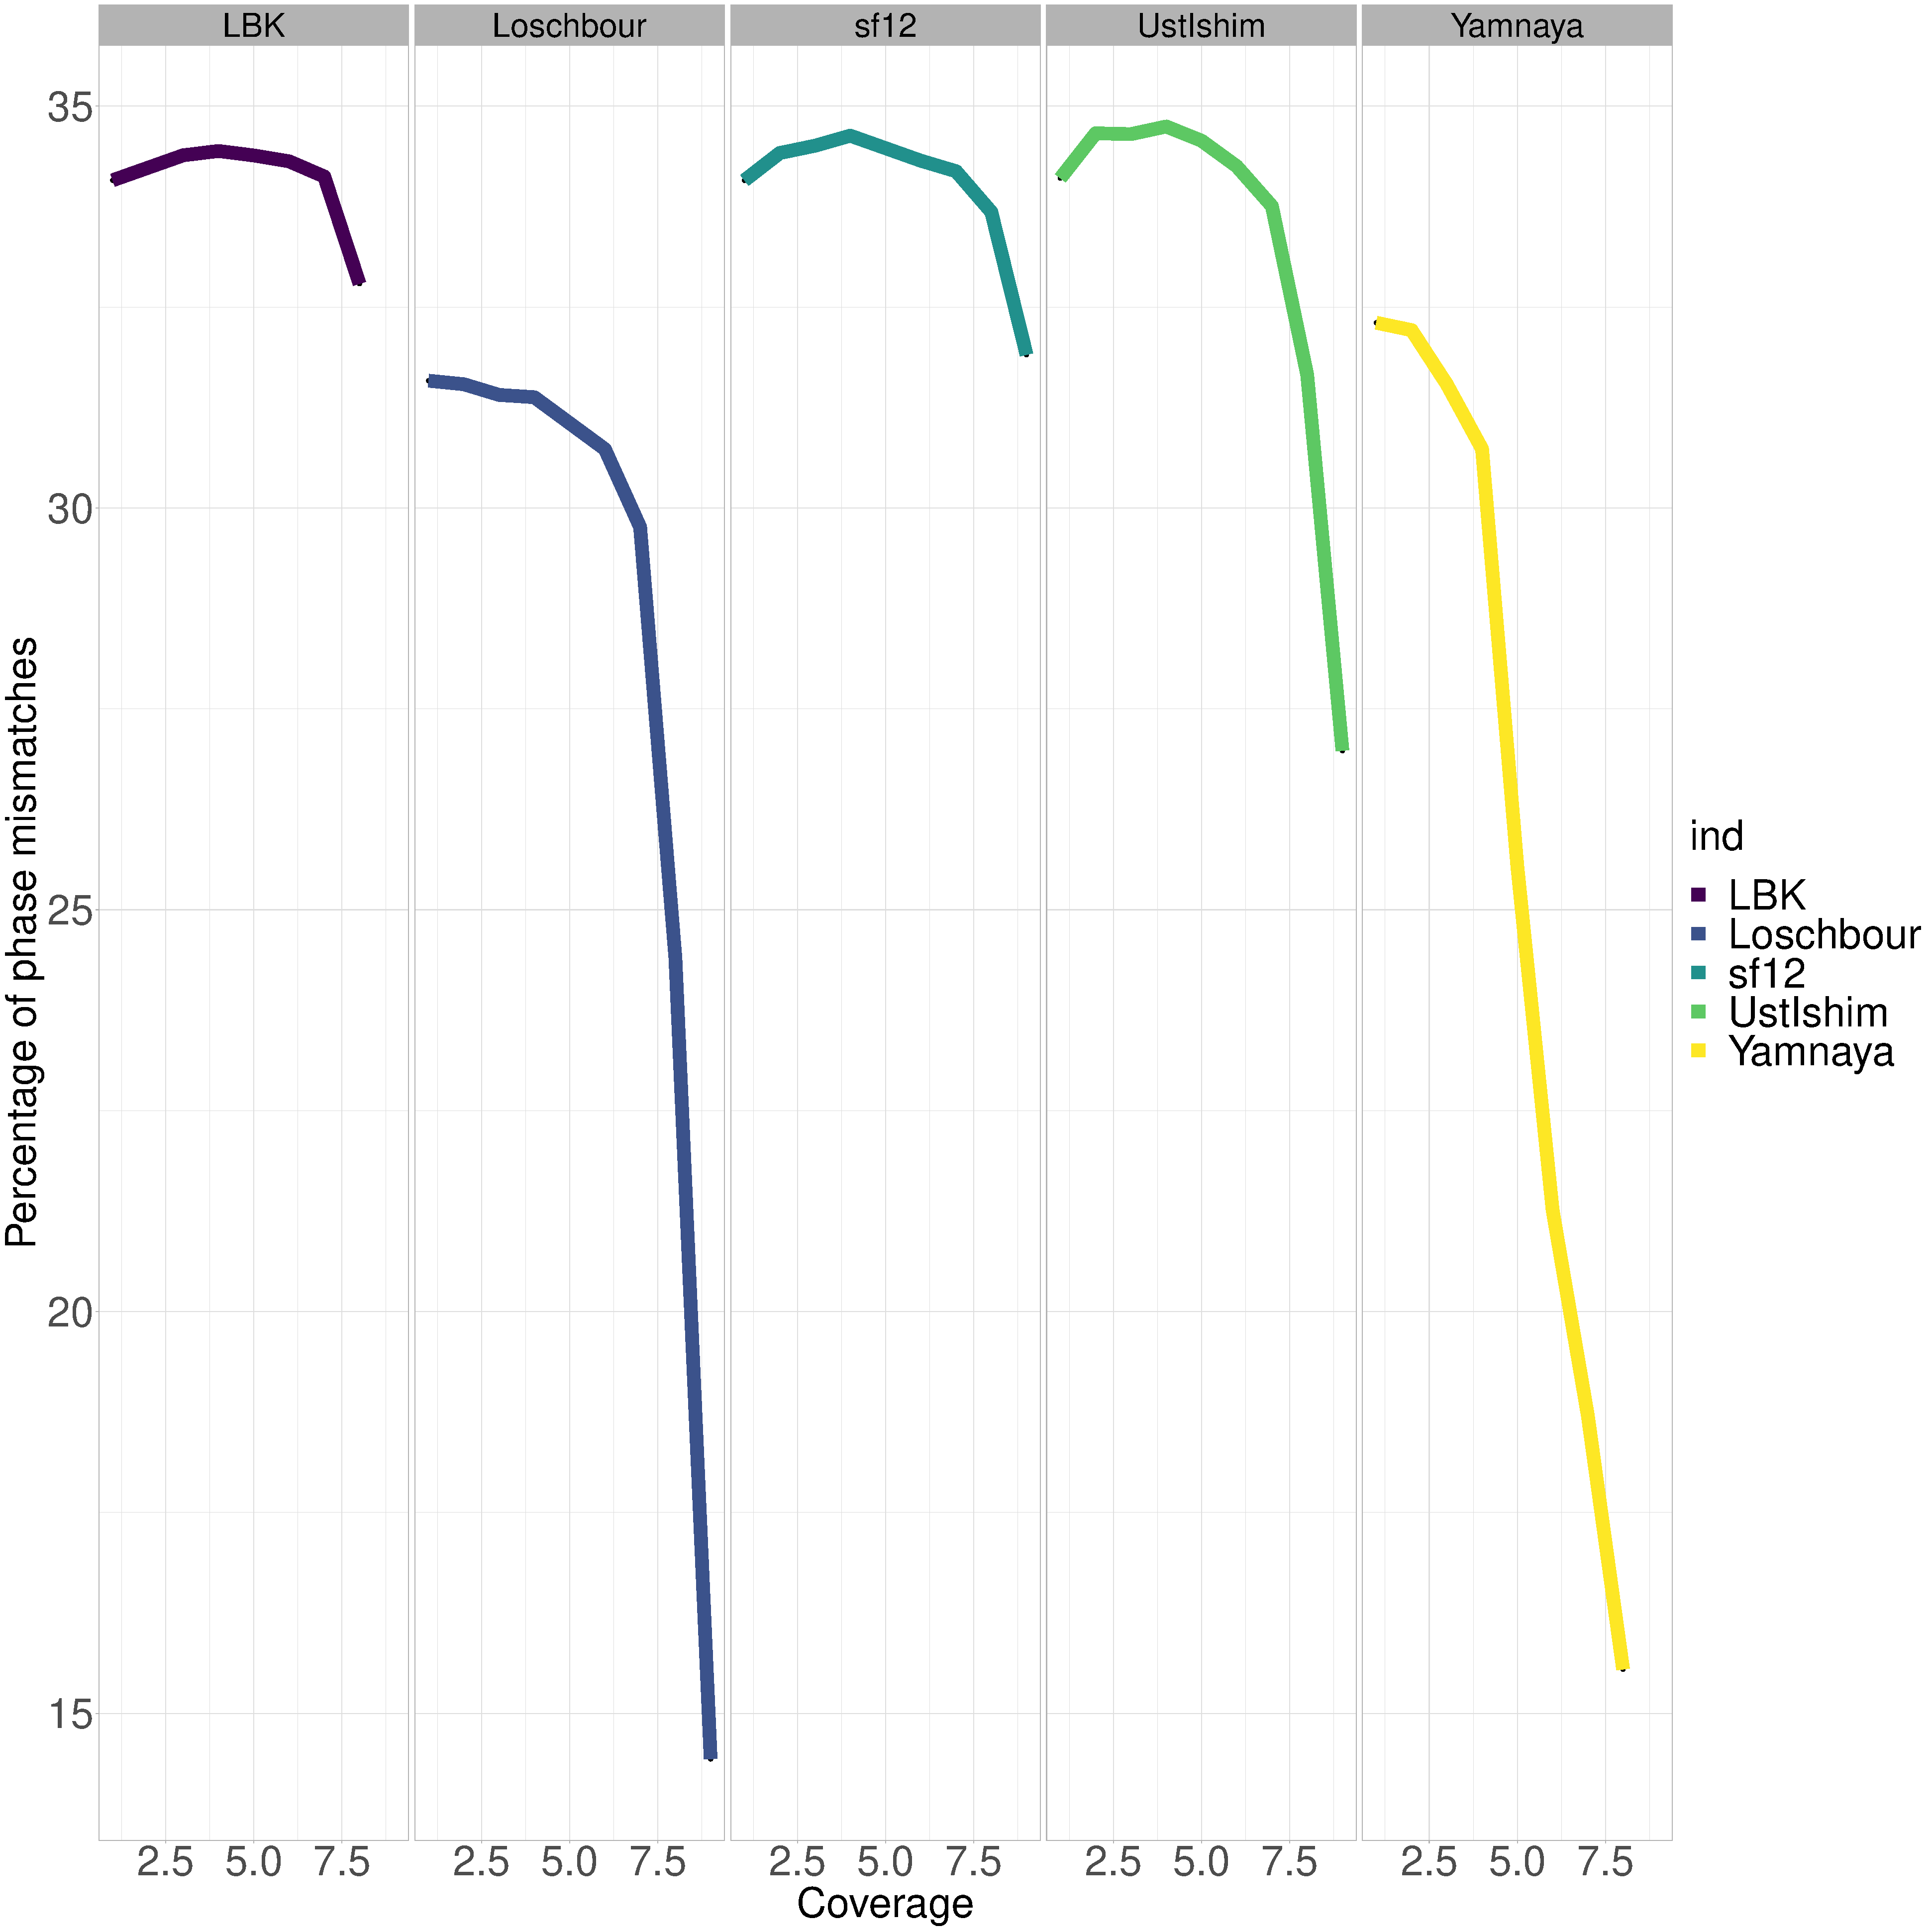
\includegraphics[width=1.0\textwidth]{../images/chapter1/phasing_performance_downsampled.pdf}
    \caption{Percentage of phased genotypes which agree with the same full-coverage sample for each individual and each level of downsampling. Genotypes with phase deemed unresolvable by rtg-tools were excluded from the calculations. Note that these numbers are given as incorrect / (incorrect + correct - unresolved) and so values are in part driven by the relative heterozygosity of each sample.}
    \label{fig:phasing_performance_downsampled}
\end{figure}

\subsection{Validating posterior probability calibration}

GLIMPSE estimates genotype probabilities at each SNP within each individual, giving the posterior probability that a given genotype within a single individual is correctly called. I assessed how well-calibrated these probabilities are in the Yamnaya 0.1x downsampled individual, using the maximum genotype likelihood at each of the approximately 77 million positions which were processed by GLIMPSE. A high $max(GL)$ for a particular genotype (i.e.\ 0.99) corresponds to a high confidence in the genotype. Alternatively a flat $max(GL)$ (i.e.\ 0.33) corresponds to no information about the genotype. 

I split the genome into 10,000 equally-sized bins according to $max(GL)$. For each bin, I calculated both the proportion of SNPs which were correctly imputed (i.e.\ that matched the same high coverage individual) and the mean $max(GL)$ (Fig. \ref{fig:Yamnaya_0.1x_GL_calibration}). If the genotype probabilities are well calibrated, we would expect to see a clear positive linear relationship between $max(GL)$ probability and the probability that genotype matches the full-coverage sample.

\begin{figure}[htp]
    \centering
    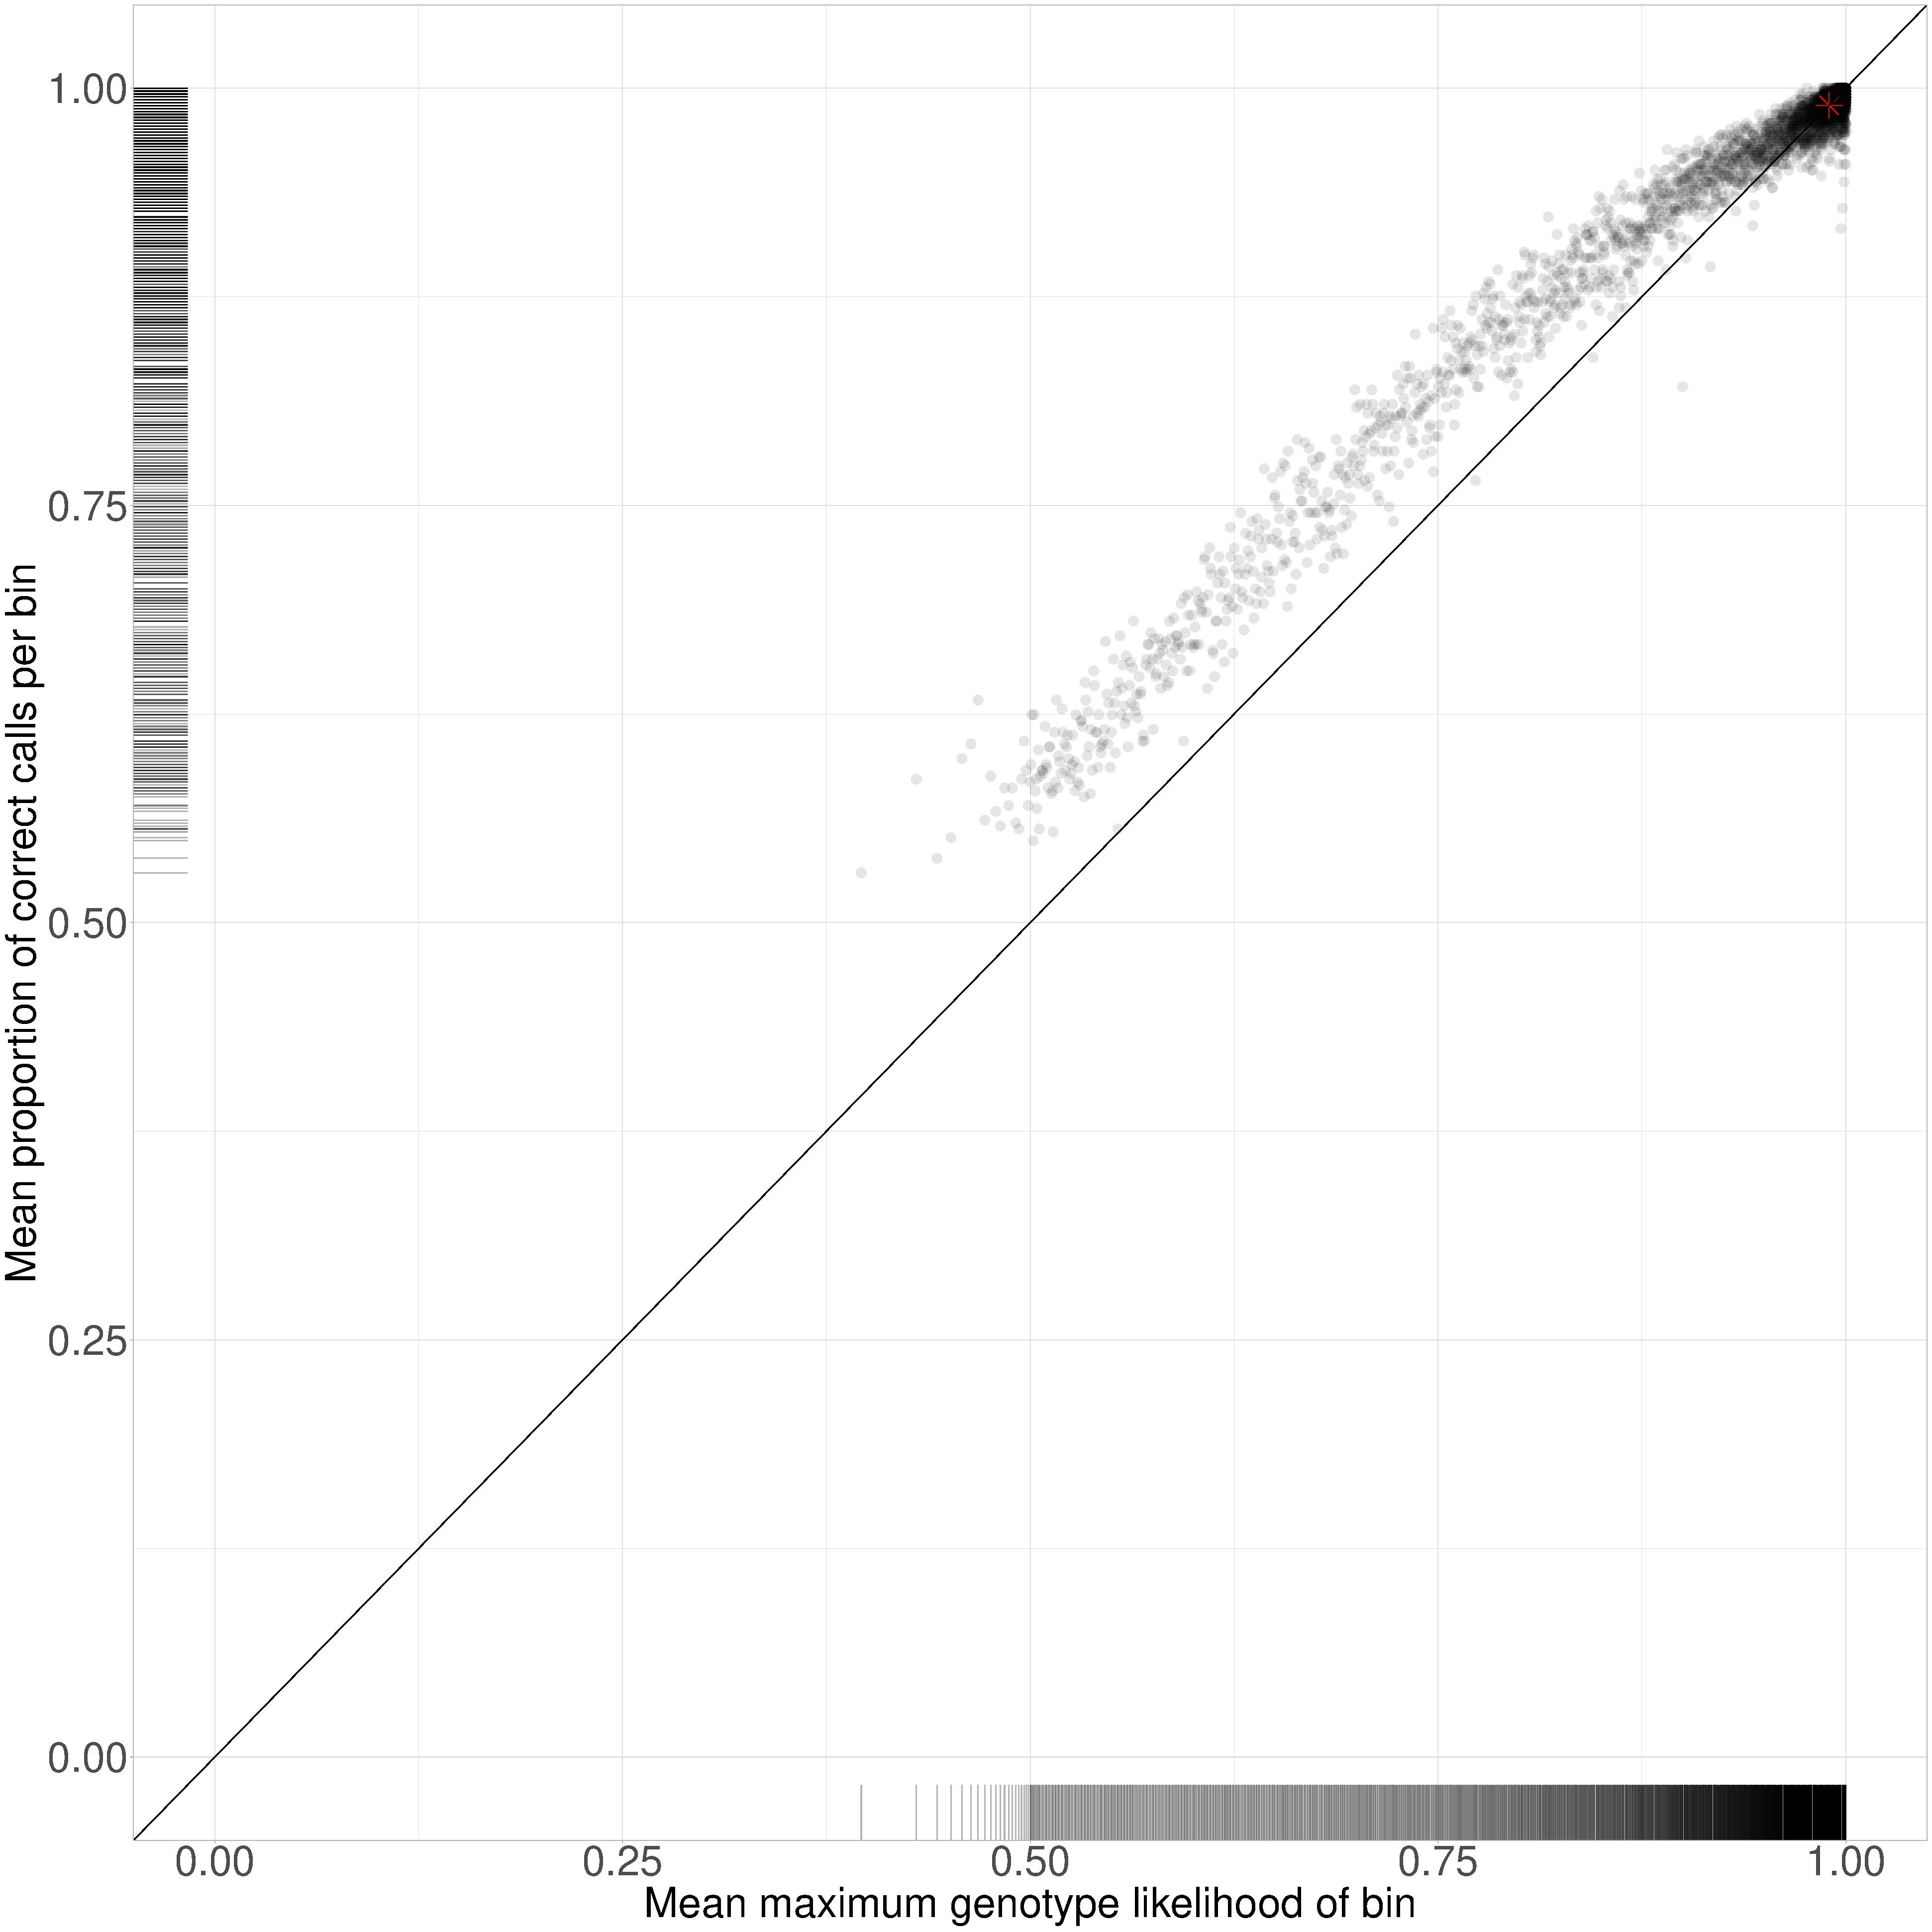
\includegraphics[width=1.0\textwidth]{../images/chapter1/Yamnaya_0.1x_bin.pdf}
    \caption{Relationship between genotype likelihood and probability of genotype call being correct for Yamnaya downsampled to 0.1x coverage. Genome binned by maximum posterior genotype likelihood and mean maximum posterior genotype likelihood (x-axis) and proportion of correct calls calculated per bin (y-axis). Rugs on each margin show the distribution of x and y values. Black line is $y=x$.}
    \label{fig:Yamnaya_0.1x_GL_calibration}
\end{figure}

The probabilities are well calibrated (r-squared = 0.981) and could therefore be useful for downstream analysis. It should be noted that they are slightly conservative, in that a majority of the points in Fig. \ref{fig:Yamnaya_0.1x_GL_calibration} are above the line of equality. For example, the mean proportion of correct genotypes within all bins where $0.73 < max(GL) < 0.76$ was 82\%. I performed the same analysis using different samples at different levels of coverage and the results were qualitatively similar (Supplementary Figure. \ref{fig:UstIshim_0.1x_bin}).

\subsection{ChromoPainter analysis} \label{sec:ChromoPainterChap2}

To assess the impact of coverage on ChromoPainter analysis, I merged the dataset of downsampled individuals with the `standard set' of ancient reference individuals (124 ancient samples $>2$X coverage) and performed an `all-v-all' painting of the merged dataset, which separately paints each individual as a recipient using all other individuals in the dataset as donors. The `all-v-all' painting was necessary to paint the 124 `standard set' of individuals against one another so that they can act as surrogates in later SOURCEFIND analysis. 

I was interested to see whether a downsampled individual and full coverage had similar copyvectors, or in other words, whether they matched similar amounts to the same donor individuals. To do this, I estimated $TVD$ between the copyvectors of the full coverage and downsampled individuals. $TVD$ is a distance metric which gives a measure of dissimilarity between two copyvectors.

Fig. \ref{fig:CP_correlation_allSamples_0.1x_0.5x_30x} displays the relationship between copyvectors for each downsampled individual and the corresponding full coverage individual for both 0.1x and 0.5x coverage. Each individuals' copyvectors were estimated using the same set of ancient samples as donors.

\begin{figure}[htp]
    \centering
    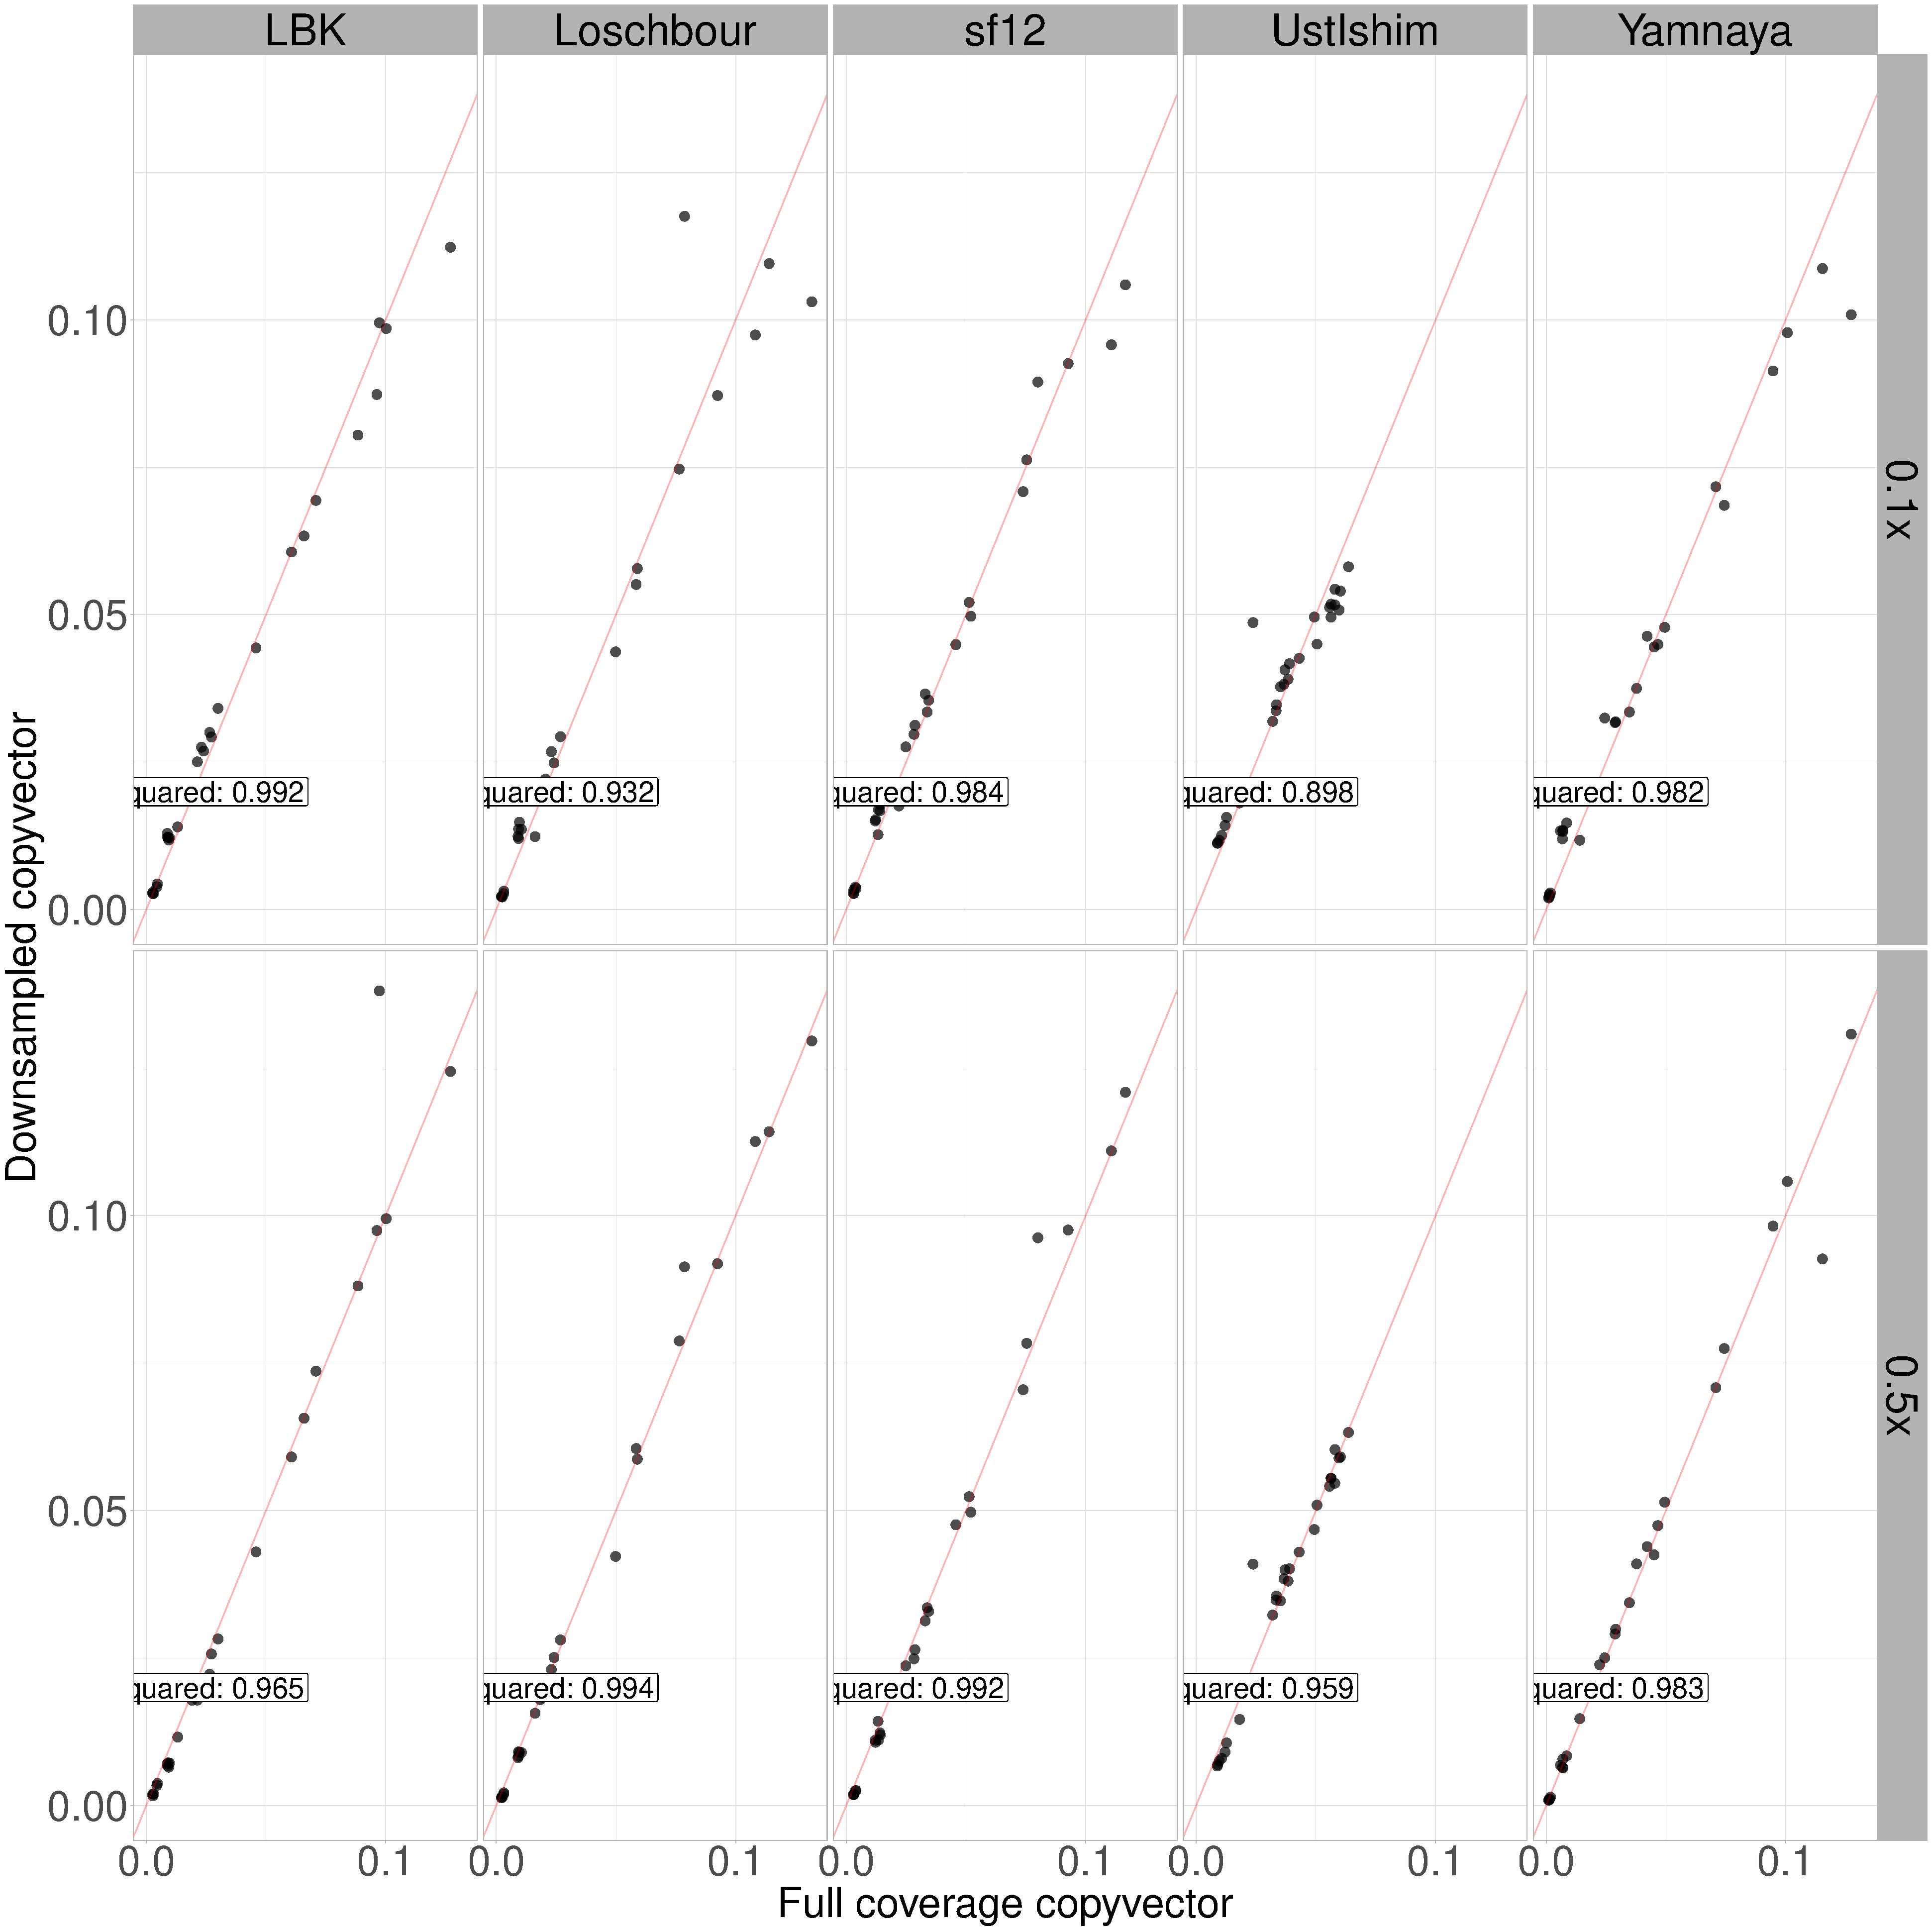
\includegraphics[width=1.0\textwidth]{../images/chapter1/CP_correlation_allSamples_0.1x_0.5x_30x.pdf}
    \caption{For five different samples (columns), the proportion of DNA that each downsampled (y-axis) or full coverage (x-axis) genome matches to each of 125 ancient individuals (dots). Results are shown for 0.1x (top row) and 0.5x (bottom row) downsampled genomes. Points coloured by manual assignment to broad-scale populations. Red line is line of equality ($y=x$). x and y units are normalised copying values and thus removed for clarity.}
    \label{fig:CP_correlation_allSamples_0.1x_0.5x_30x}
\end{figure}

As expected, the TVD between the full-coverage and downsampled copyvectors decreased with coverage. The 0.1x genome had a substantially increased TVD, similar to the much reduced imputation accuracy. For each of the genomes downsampled to 0.1x, a particular difference to the 0.5x downsampled genomes is that the lowest contributing donors contribute more to the 0.1x downsampled genome than to the full coverage genome and that the highest contributing donors contribute less to the 0.1x genome than they do the full coverage genome. Put in other words, the copyvectors at 0.1x are tending towards becoming more `flat', or copying the same amount from each donor individual. 

This can also be seen as `regressing to the prior'. In this case, the prior is copying an equal amount to each donor individual. This can be visualised explicitly by calculating TVD between each downsampled genome and a flat prior, a vector of length $D$, where $D$ is the total number of donor individuals and each element of $D$ is equal to 1 / $D$ (Fig. \ref{fig:TVD_ancients_flat_prior}). This clearly shows the reduced TVD to the flat copyvector for the 0.1x individual relative to other coverages. In later sections, I will discuss whether this is `noise' or `bias' induced by imputation, i.e.  whether copying is regressing to the prior in a similar manner for all samples. 

\begin{figure}[htp]
    \centering
    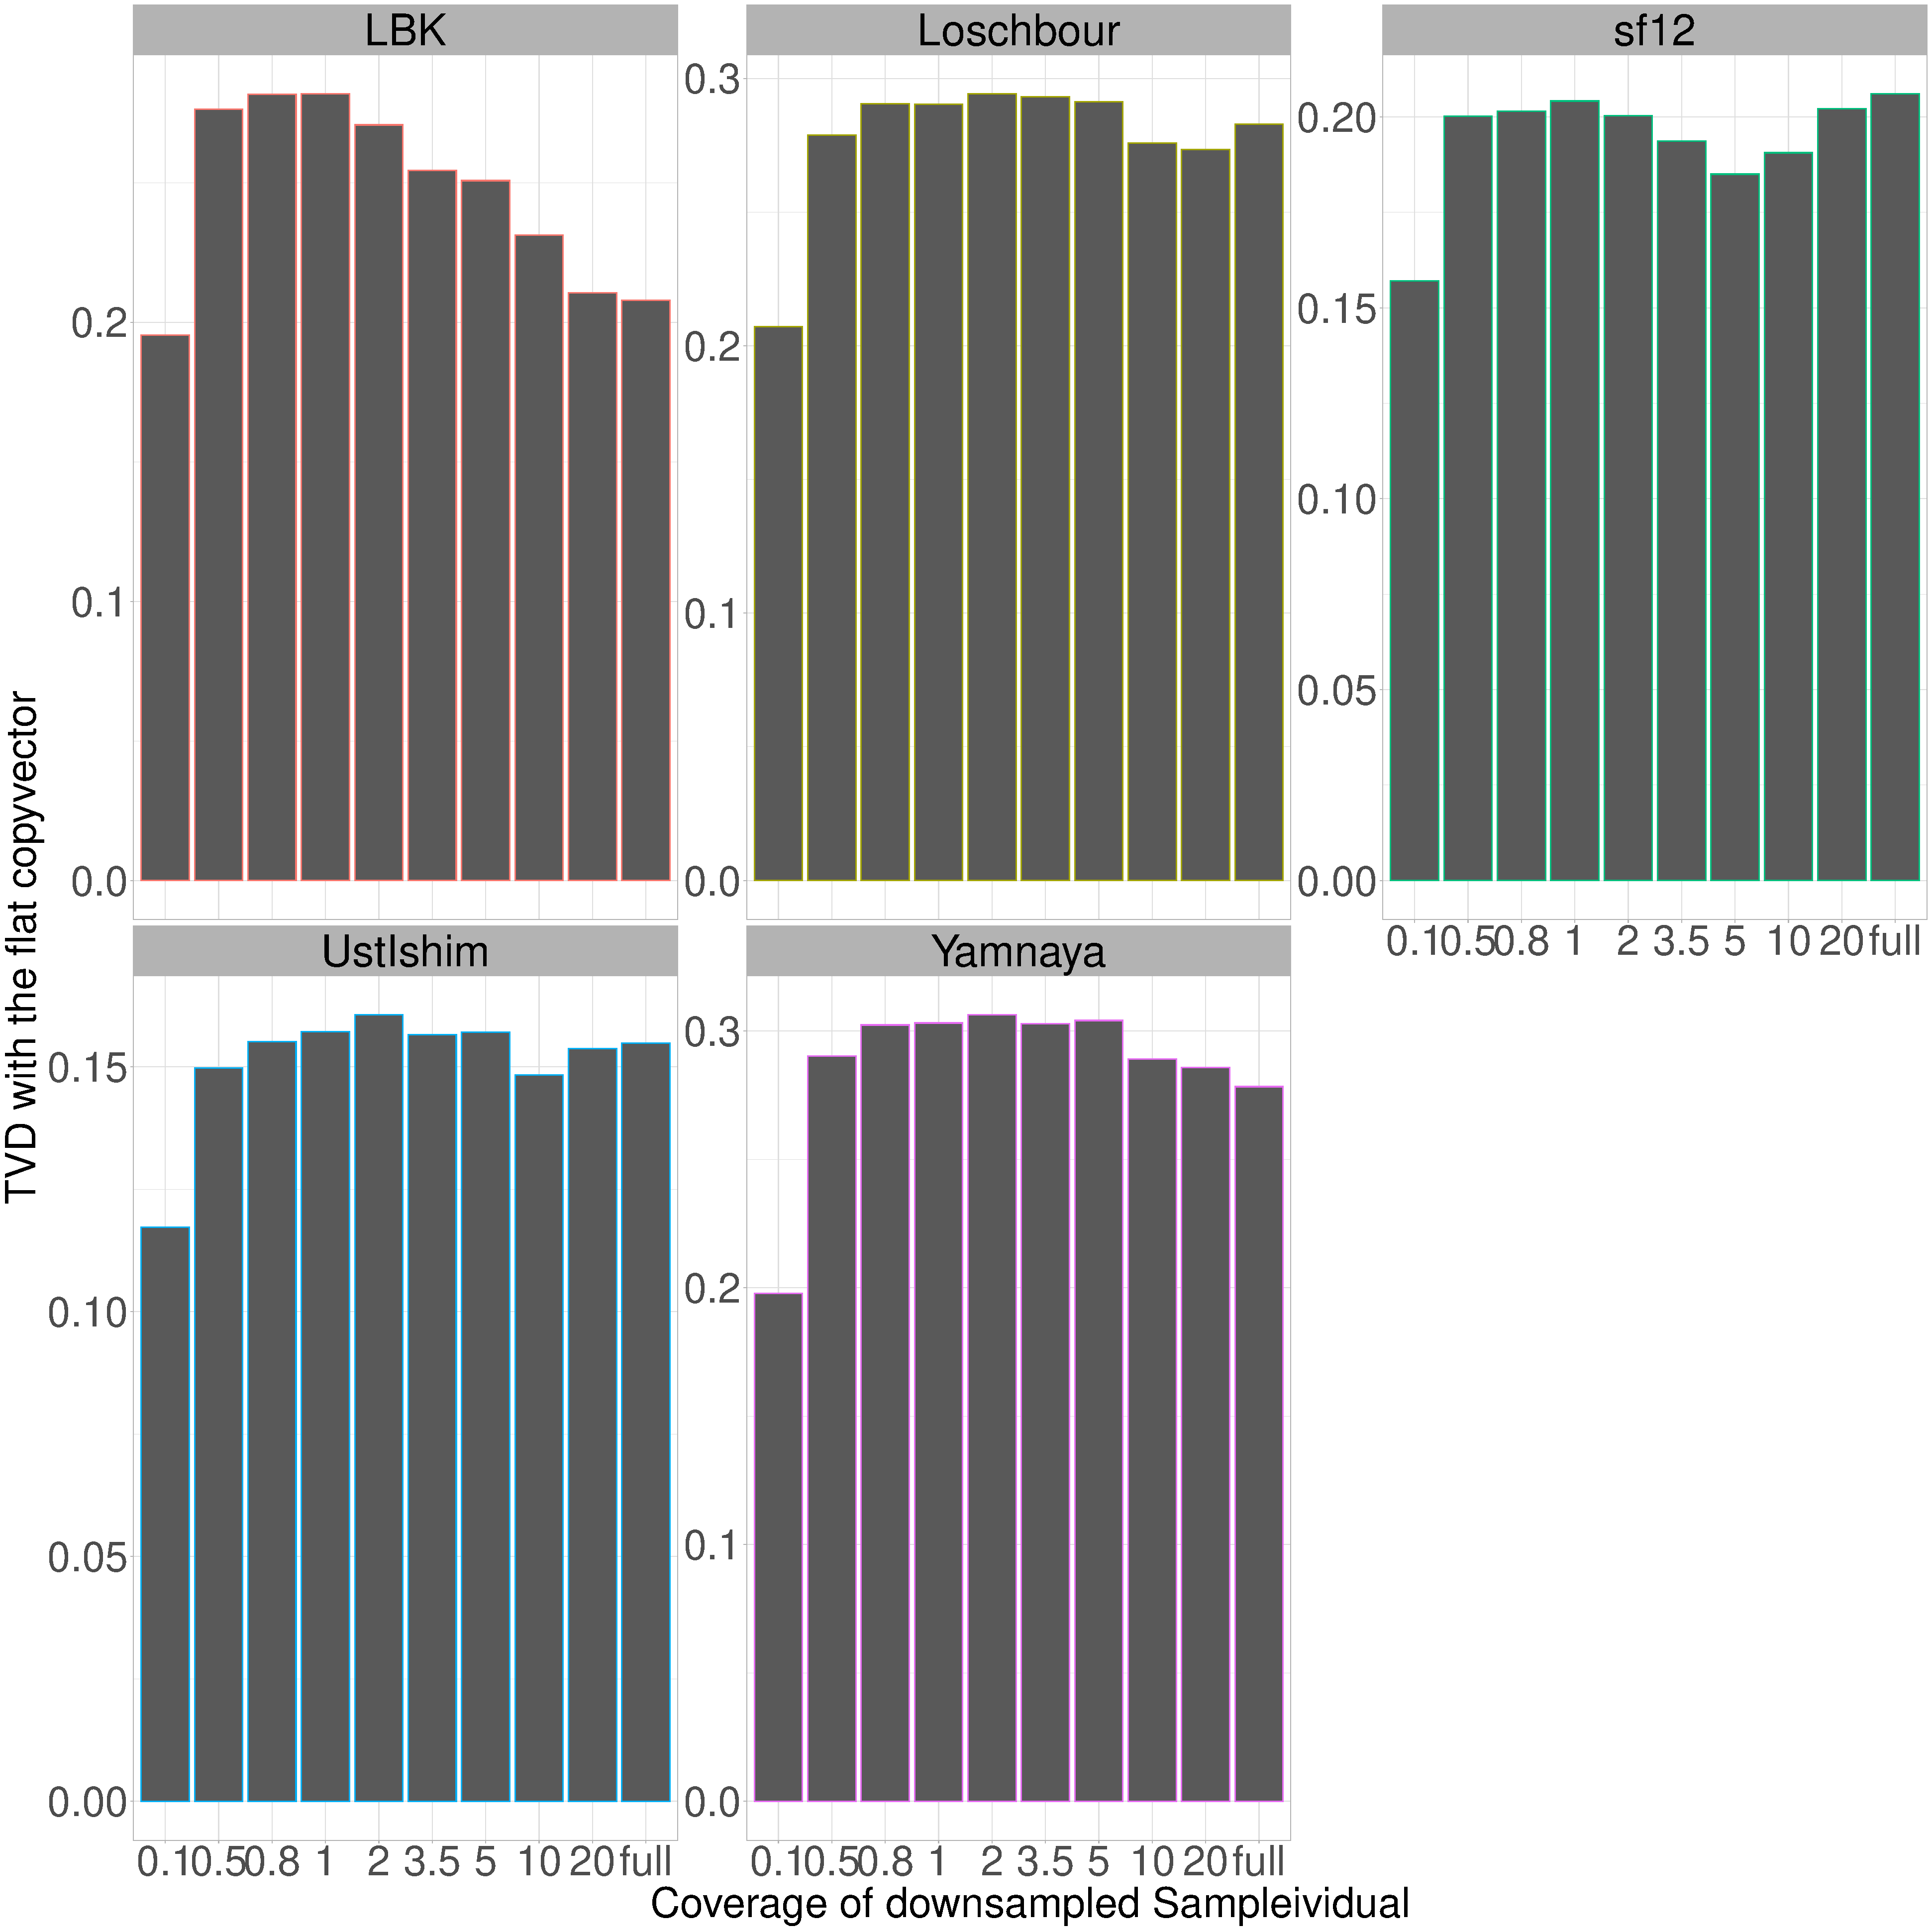
\includegraphics[width=1.0\textwidth]{../images/chapter1/TVD_ancients_flat_prior.pdf}
    \caption{TVD (metric of copyvector dissimilarity between two individuals) between each downsampled ancient individual and a flat copyvector. Flat copyvector equivalent to a vector of length $N$ where each element = $1/N$.}
    \label{fig:TVD_ancients_flat_prior}
\end{figure}

I also considered the effect of coverage on the copyvectors estimated when using present-day individuals from the 1000 genomes project as donors (Fig. \ref{fig:CP_correlation_allSamples_0.1x_0.5x_30x_moderns}). Painting ancient samples using present-day donors is often useful, particularly with more recent ancient samples, as there may not be enough relevant ancient samples to paint the ancients with. I merged the downsampled and full coverage ancient individuals with the thousand genomes dataset (described in detail in Appendix section \ref{section:1000genomes}). As was the case with the all-v-all ancients painting, the TVD between copyvectors was highest for the 0.1x individuals. However, the copyvectors show a strong correlation / low TVD for 0.5x individuals. 

It should be noted that utility of painting different ancient individuals with a modern reference panel depends on the ancestry and age of the ancient sample. The spread of points along the $y=x$ line in Fig. \ref{fig:CP_correlation_allSamples_0.1x_0.5x_30x_moderns} shows how much a particular ancient recipient preferentially copies more from particular modern population over others. LBK, for example, has points which are spread evenly across $y=x$, showing that they copy much more from some populations than others, suggesting modern populations are good for distinguishing this particular ancient sample. On the other hand, the points for Ust'Ishim are shrunk towards lower values of $y=x$, showing that the copyvector is relatively flat and that it does not preferentially copy from some populations to the same degree that LBK does. This is consistent with findings that UstIshim did not contribute ancestry towards present-day populations \cite{Fu2014}. Accordingly, relatively less useful information is obtained from painting Ust'Ishim with a modern reference panel than LBK.

\begin{figure}[htp]
    \centering
    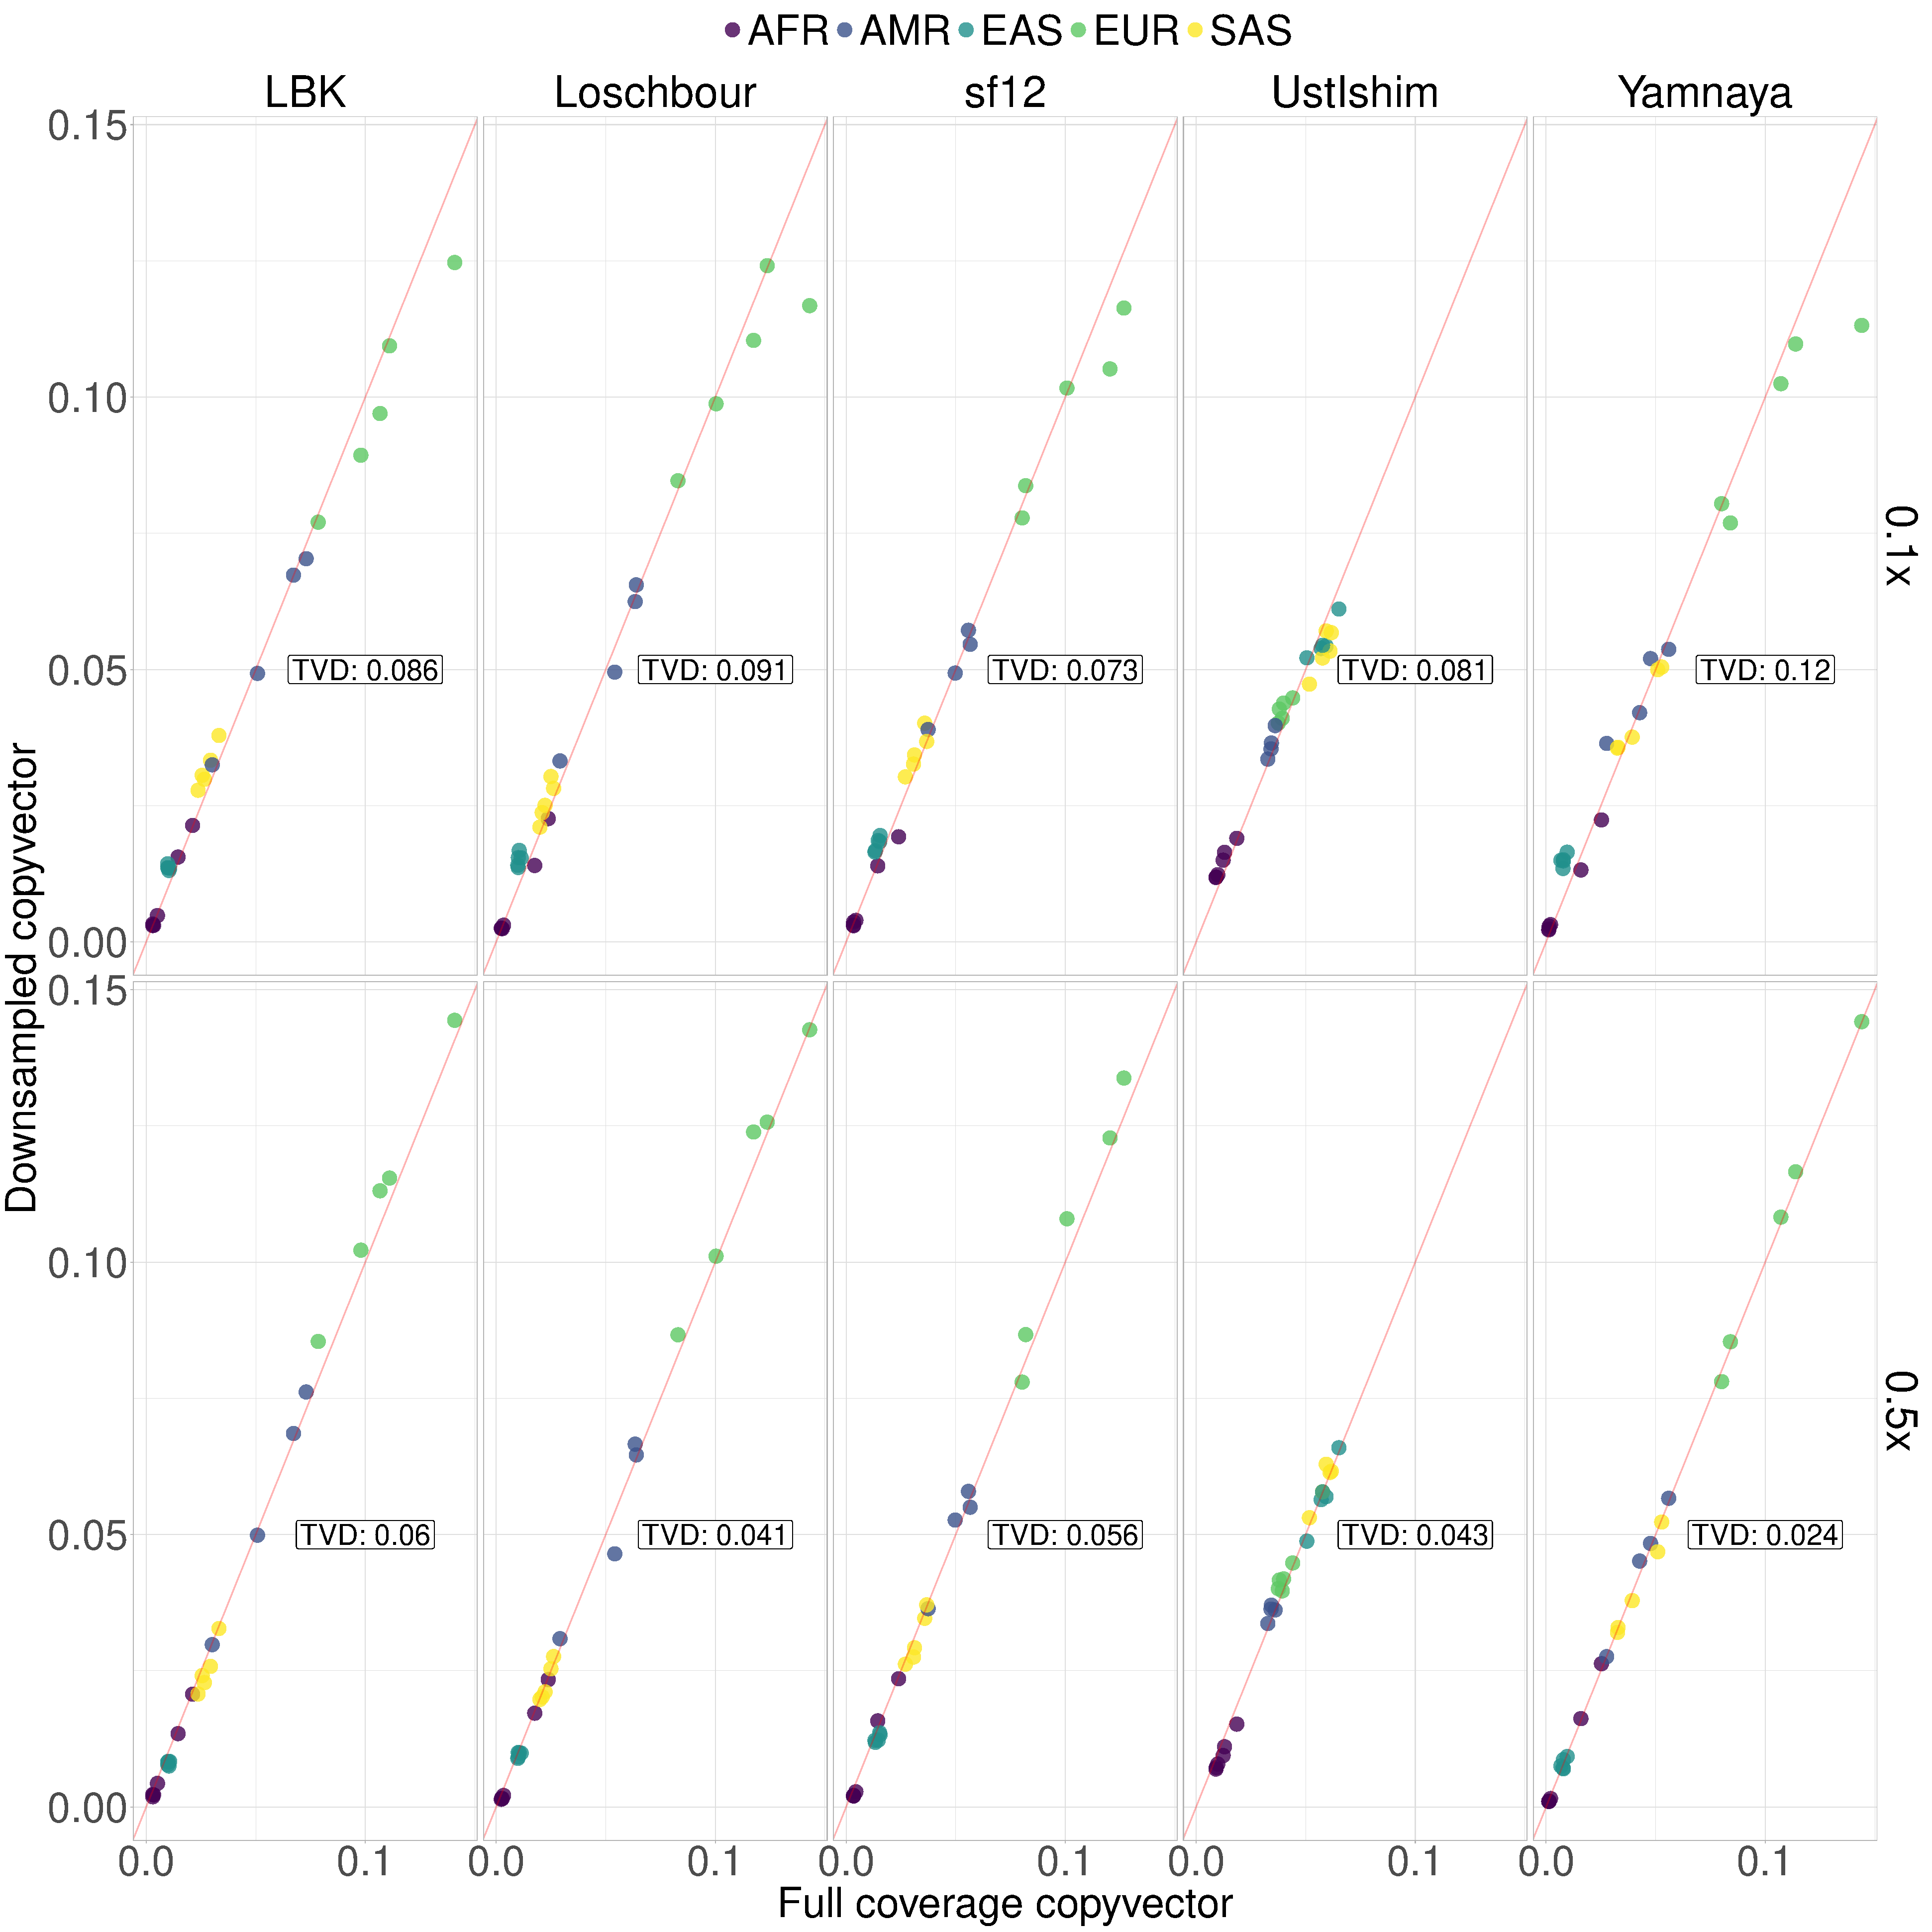
\includegraphics[width=1.0\textwidth]{../images/chapter1/CP_correlation_allSamples_0.1x_0.5x_30x_moderns.pdf}
    \caption{For five different samples (columns), the proportion of DNA that each downsampled (y-axis) or full coverage (x-axis) genome matches to individuals from each of 26 present-day populations (dots). Red line is $y=x$. x and y units are normalised copying values and thus removed for clarity. Points coloured by meta-population.}
    \label{fig:CP_correlation_allSamples_0.1x_0.5x_30x_moderns}
\end{figure}

Principle component analysis (PCA) is a widely used technique to visualise the relative genetic diversity of different individuals. PCA can be performed on the chunklengths matrix in a similar way to how PCA on the genotype dosage matrix is often employed in ancient DNA studies. Visualising whether downsampled individuals cluster close to the same sample at full-coverage is a useful way of determining whether the copyvectors of the downsampled individual reflect those of the full-coverage individual.

The position of the full coverage individuals are consistent with prior knowledge about their ancestry (Fig. \ref{fig:PCA_panel_allInds_allCoverage}). For example, Loschbour is positioned alongside other Hunter Gatherers, who are highly differentiated from the later Neolithic farmers and Bronze Age Europeans. sf12 clusters with the other Scandinavian Hunter Gatherers in the dataset. Yamnaya is differentiated from the group of Bronze Age individuals and situated close to individuals from the Poltavka and Srubnaya culture. LBK is located with other individuals from the early to middle Neolithic in central Europe. Consistent with sharing little ancestry with any group over another, UstIshim is positioned close to the central Bronze Age mass, where most of the individuals in the PCA are located. 

For all levels of downsampling other than the 0.1x, the downsampled and full coverage genomes were positioned very closely to one another on the PCA. When considering all downsampled individuals, a pattern emerges whereby the genome downsampled to 0.1x for each individual is `pulled' towards the origin of the PCA. This may reflect a `homogenisation' of low coverage genomes when many genotypes are imputed.

To formally examine the positioning of the samples on the PCA, I calculated the closest Cartesian neighbour to each of the downsampled individuals, not including other downsampled individuals (Table \ref{tab:ClosestNeighbour}). Other than at 0.1x coverage, the samples UstIshim, sf12 and Loschbour always were closest to the same sample at full coverage. Up to 5x coverage, Yamnaya was closest to closely related YamnayaSamara and Poltavka samples. 


\begin{figure}[htp]
    \centering
    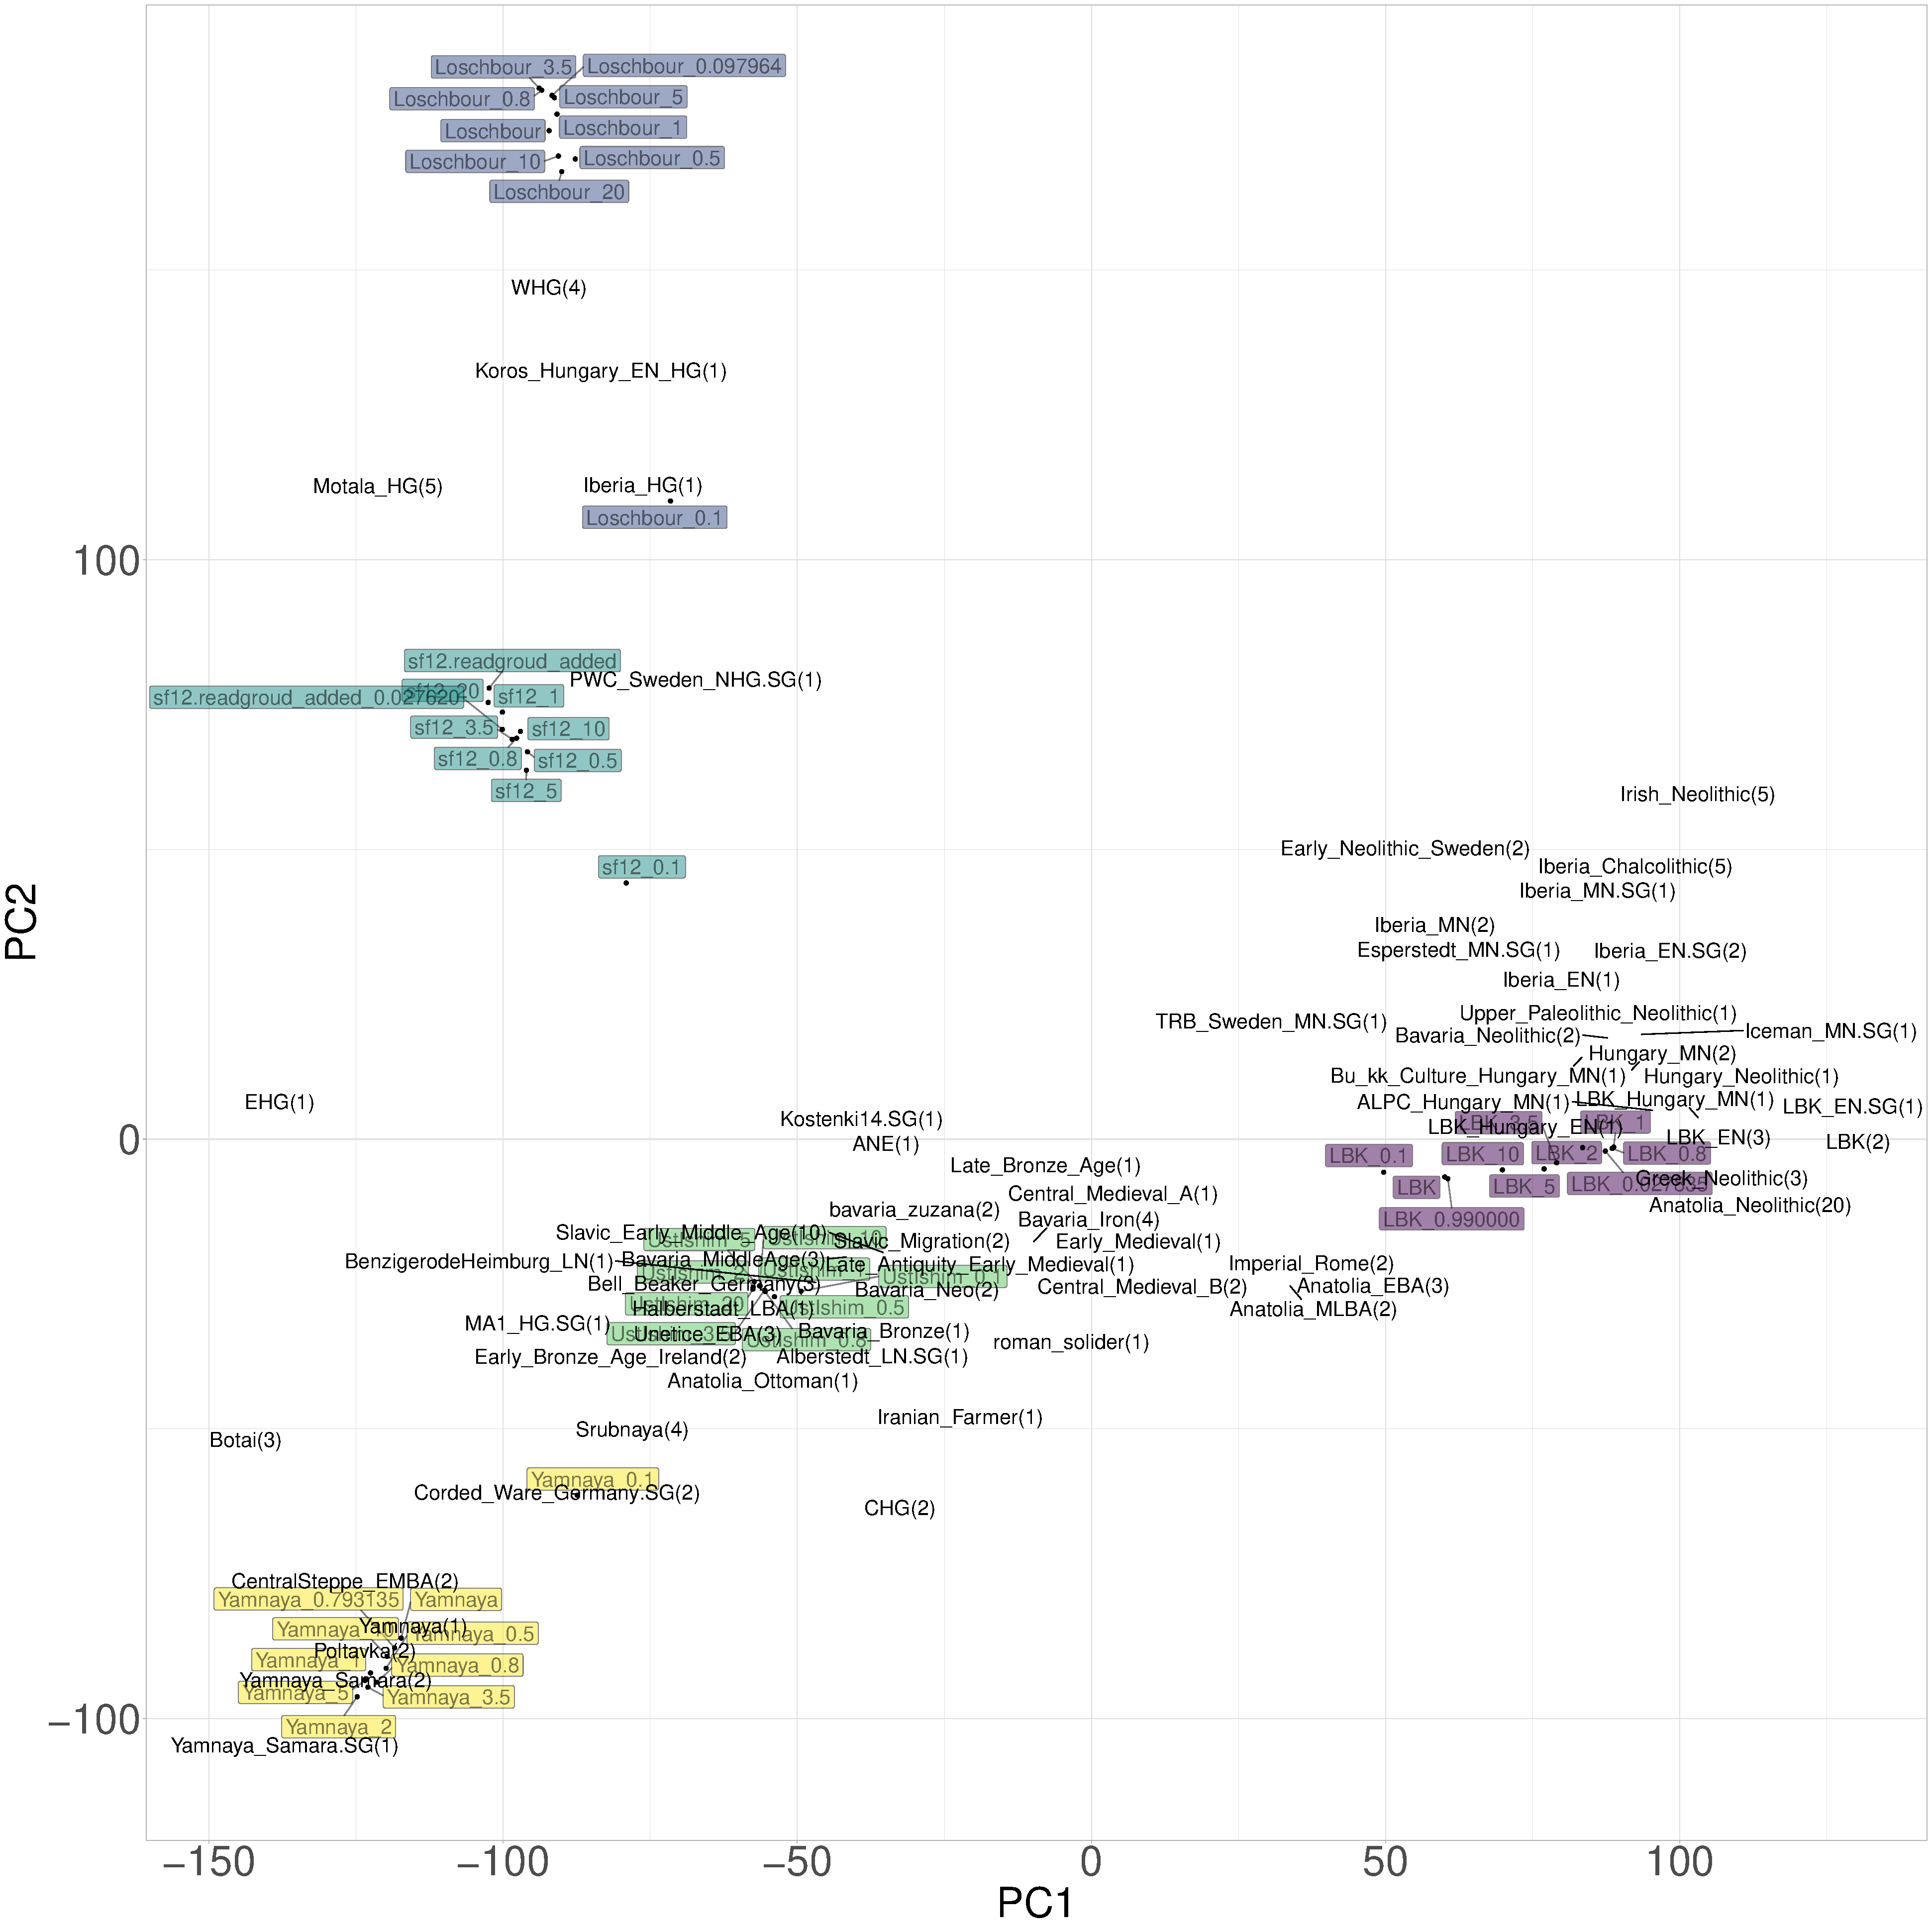
\includegraphics[width=1.0\textwidth]{../images/chapter1/PCA_panel_allInds.allCoverage.pdf}
    \caption{Principle component analysis (PCA) of downsampled, full coverage and downloaded ancient individuals generated from the linked chunklengths matrix. Full coverage and downsampled genomes of the same individual are coloured the same. Reference individuals are grouped into populations plotted as the mean principle components for all individuals within the population. Numbers in labels correspond to the number of individuals within the reference population. 0.1x samples have red border for clarity.}
    \label{fig:PCA_panel_allInds_allCoverage}
\end{figure}

\begin{table}
\centering
\begin{tabular}[t]{lllll}
\toprule
Coverage & Loschbour & sf12 & UstIshim & Yamnaya\\
\midrule
0.1 & Iberia\_HG & PWC\_SwedenNHG.SG & BHeimburg\_LN & CordedWare\\
0.5 & Loschbour & sf12 & UstIshim & Poltavka\\
0.8 & Loschbour & sf12 & UstIshim & Poltavka\\
1 & Loschbour & sf12 & UstIshim & Poltavka\\
2 & Loschbour & sf12 & UstIshim & YamnayaSamara\\
3.5 & Loschbour & sf12 & UstIshim & YamnayaSamara\\
5 & Loschbour & sf12 & UstIshim & YamnayaSamara\\
10 & Loschbour & sf12 & UstIshim & Yamnaya\\
20 & Loschbour & sf12 & UstIshim & Yamnaya\\
\bottomrule
\end{tabular}
\caption{For each downsampled individual at each level of coverage, each entry gives the closest Cartesian neighbour based upon the PCA in Fig \ref{fig:PCA_panel_allInds_allCoverage}, not including other downsamples.}
\label{tab:ClosestNeighbour}
\end{table}


Taken together, this data suggests a minimal effect of coverage down to and including 0.5x mean depth. To my knowledge, no other study has evaluated the effect of coverage on ChromoPainter analysis down to a coverage of 0.5x. Using Beagle v4/v4.1, Margaryan et al (2020) showed a minimal effect of coverage at 1x and that fineSTRUCTURE groupings, containing individuals as low as 0.5x coverage, were not driven by coverage \cite{margaryan2020population}. 


\subsection{SOURCEFIND}

I next determined the effect of sequencing coverage on the ancestry proportions estimated by SOURCEFIND, which accounts for variable donor group sizes and incomplete lineage sorting  to improve interpretability relative to the raw chunklengths matrix.

I began by considering three ancestral sources, or `surrogates', fixed as Anatolia Neolithic, Western Hunter-Gatherer and Yamnaya steppe pastoralist. I compared inferred proportions for the same individual across different levels of coverage (Fig. \ref{fig:3pop_SF_downsampled}). 

\begin{figure}[htp]
    \centering
    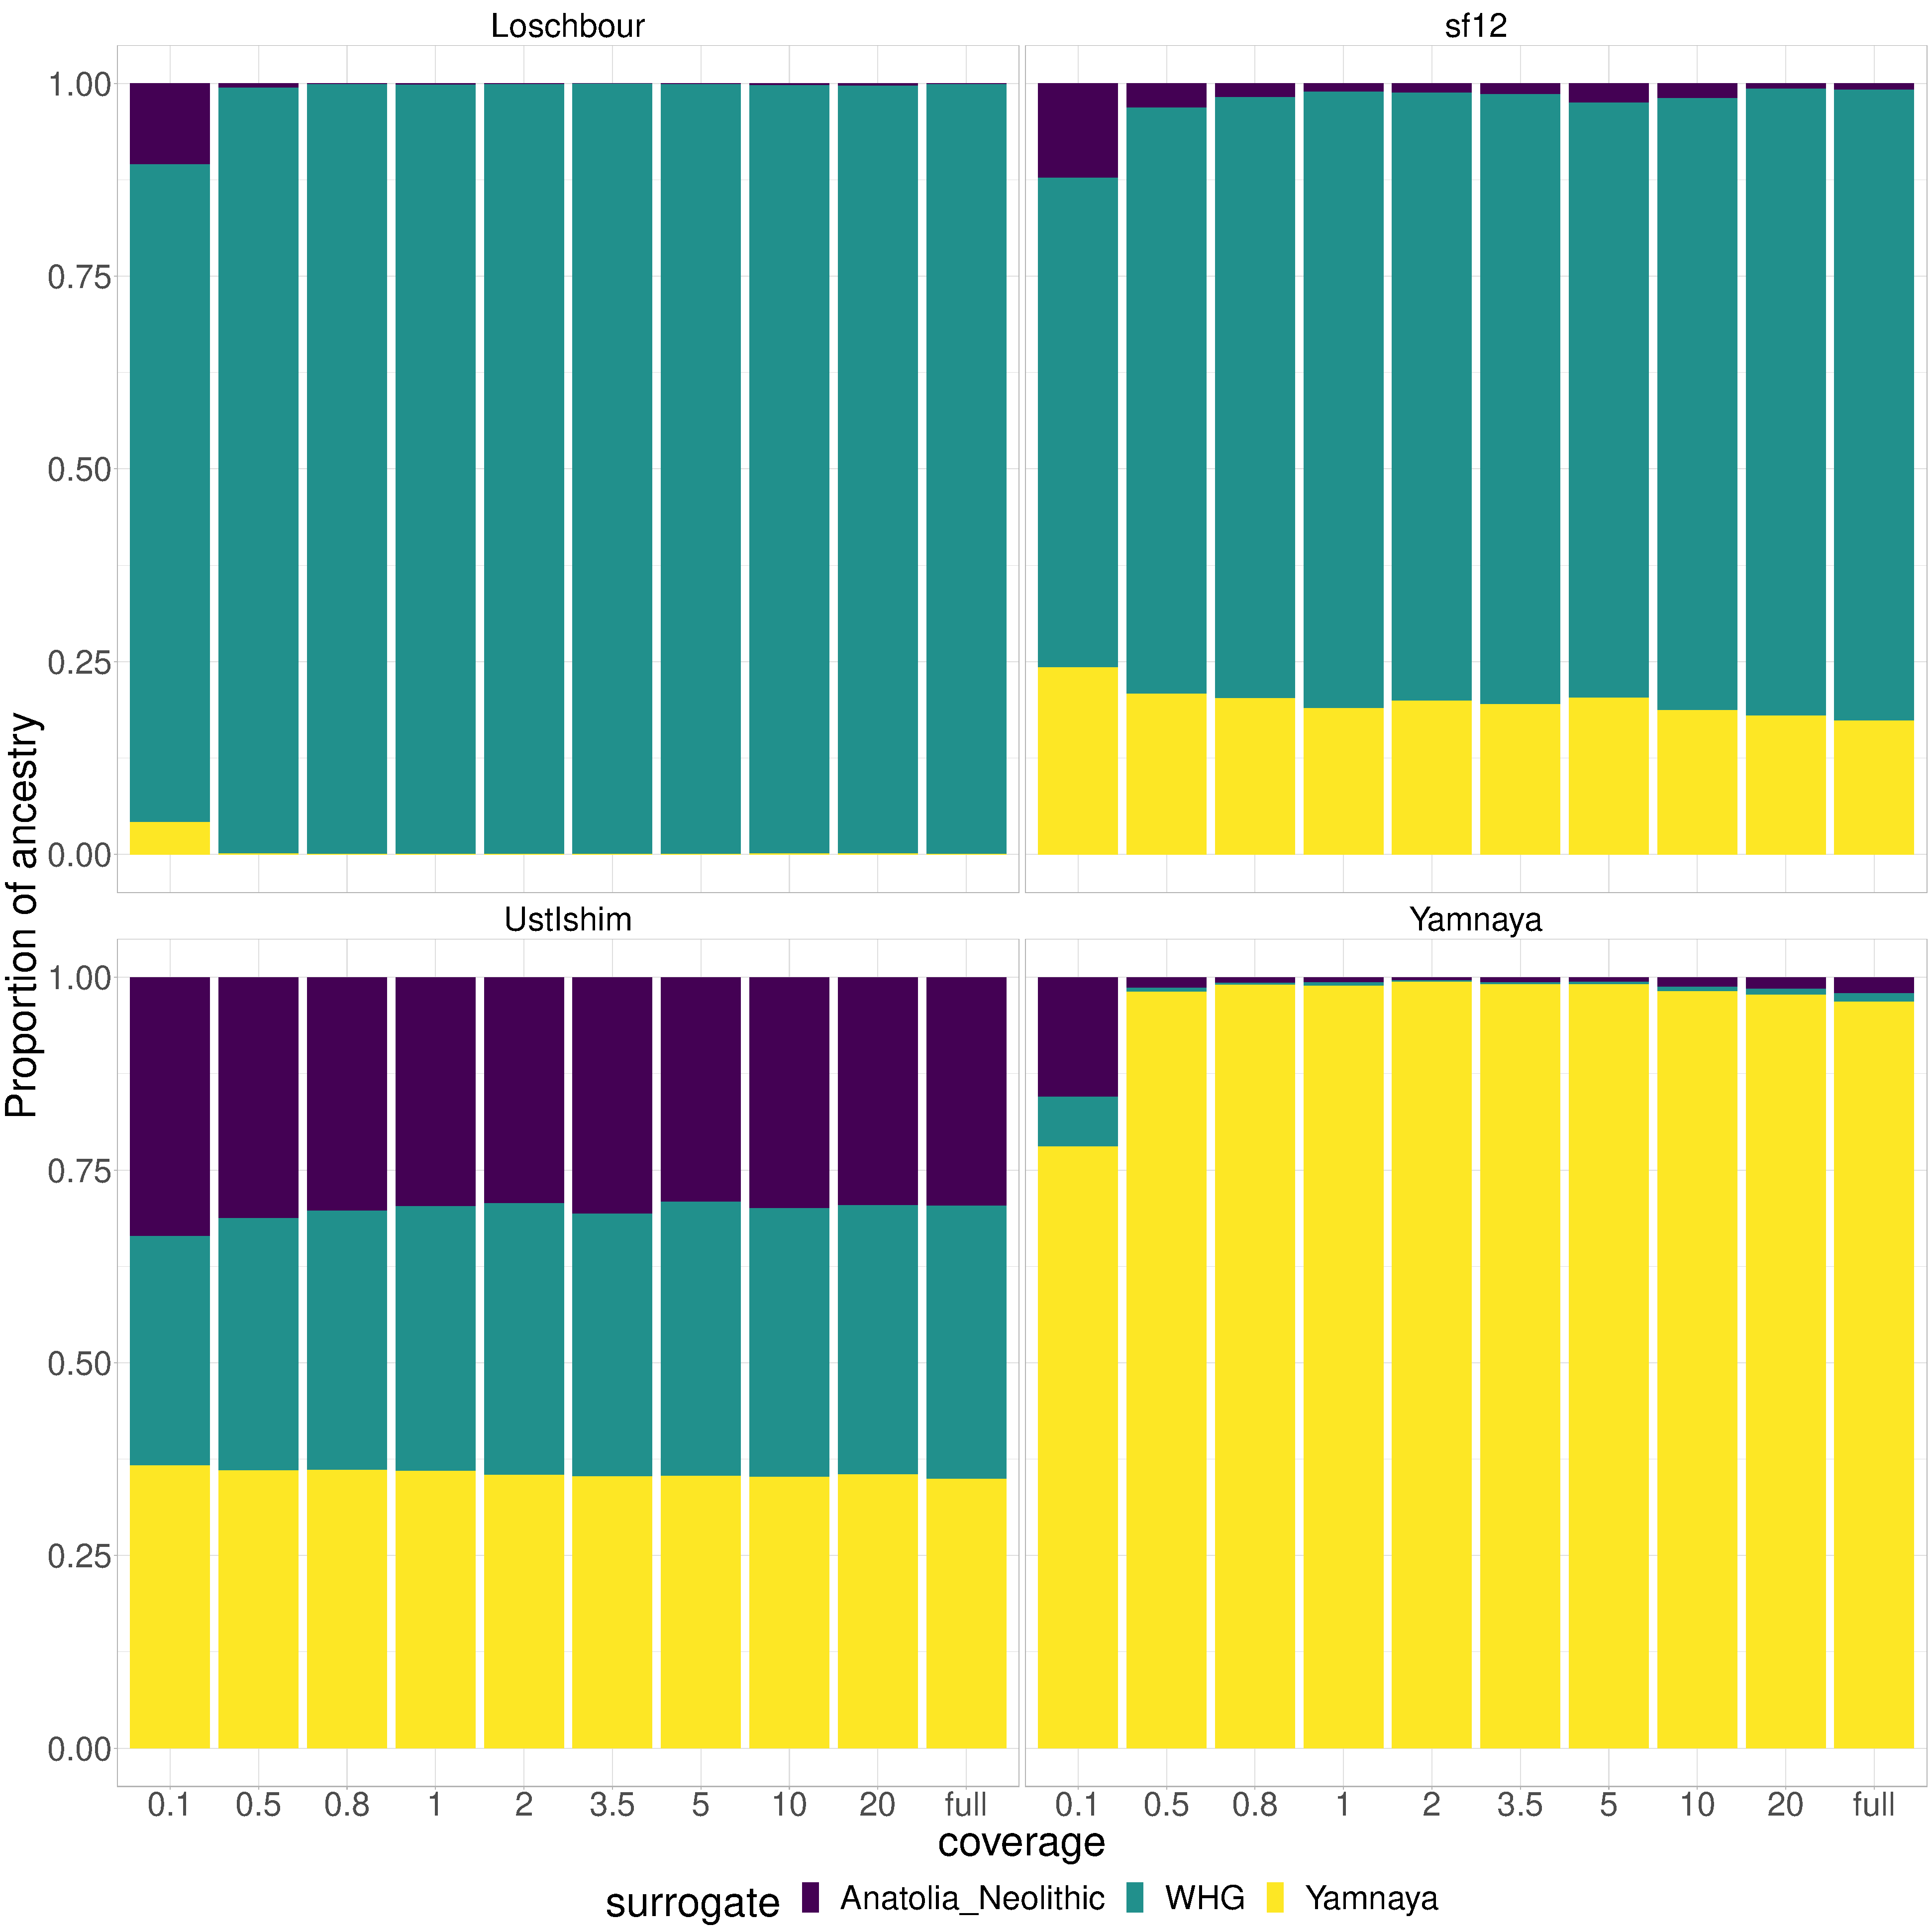
\includegraphics[width=1.0\textwidth]{../images/chapter1/3pop_SF_downsampled.pdf}
    \caption{Each panel gives SOURCEFIND inferred recent ancestry sharing proportions for a different downsampled genome. Bars represent proportion of ancestry, coloured by different surrogates. Different coverages for the same individual are given within each panel. Three surrogates were used.}
    \label{fig:3pop_SF_downsampled}
\end{figure}

Consistent with previous results, SOURCEFIND estimates are robust down to 0.5-0.8x coverage. At 0.1x coverage, there is an increase in ancestry components that are not present in higher coverage samples, suggesting they are artefacts caused by low coverage. For example, small components of Anatolia Neolithic and Yamnaya ancestry appear in Loschbour at 0.1x coverage, which are not present at any higher coverages. Above 0.5x coverage, the effect of coverage on estimated ancestry proportions appears to be marginal. For example, in sf12, the difference in the minor ancestry component of Anatolia Neolithic is, at most, 2.4\%. LBK was excluded because downsamples had anomalously poor results; I inferred roughly equal proportions of all surrogates in spite of the fact that they should have been almost 100\% farmer. 

However, more than three surrogates are often used, as SOURCEFIND is meant to infer the most important contributors without \textit{a priori} knowledge of the samples' ancestry. Therefore, I re-ran SOURCEFIND using 39 surrogate populations (Fig. \ref{fig:SOURCEFIND_AllPSop_downsampled}). For all downsamples above 0.1x in coverage, the ordering of proportions for each surrogate was the same. 

\begin{figure}[htp]
    \centering
    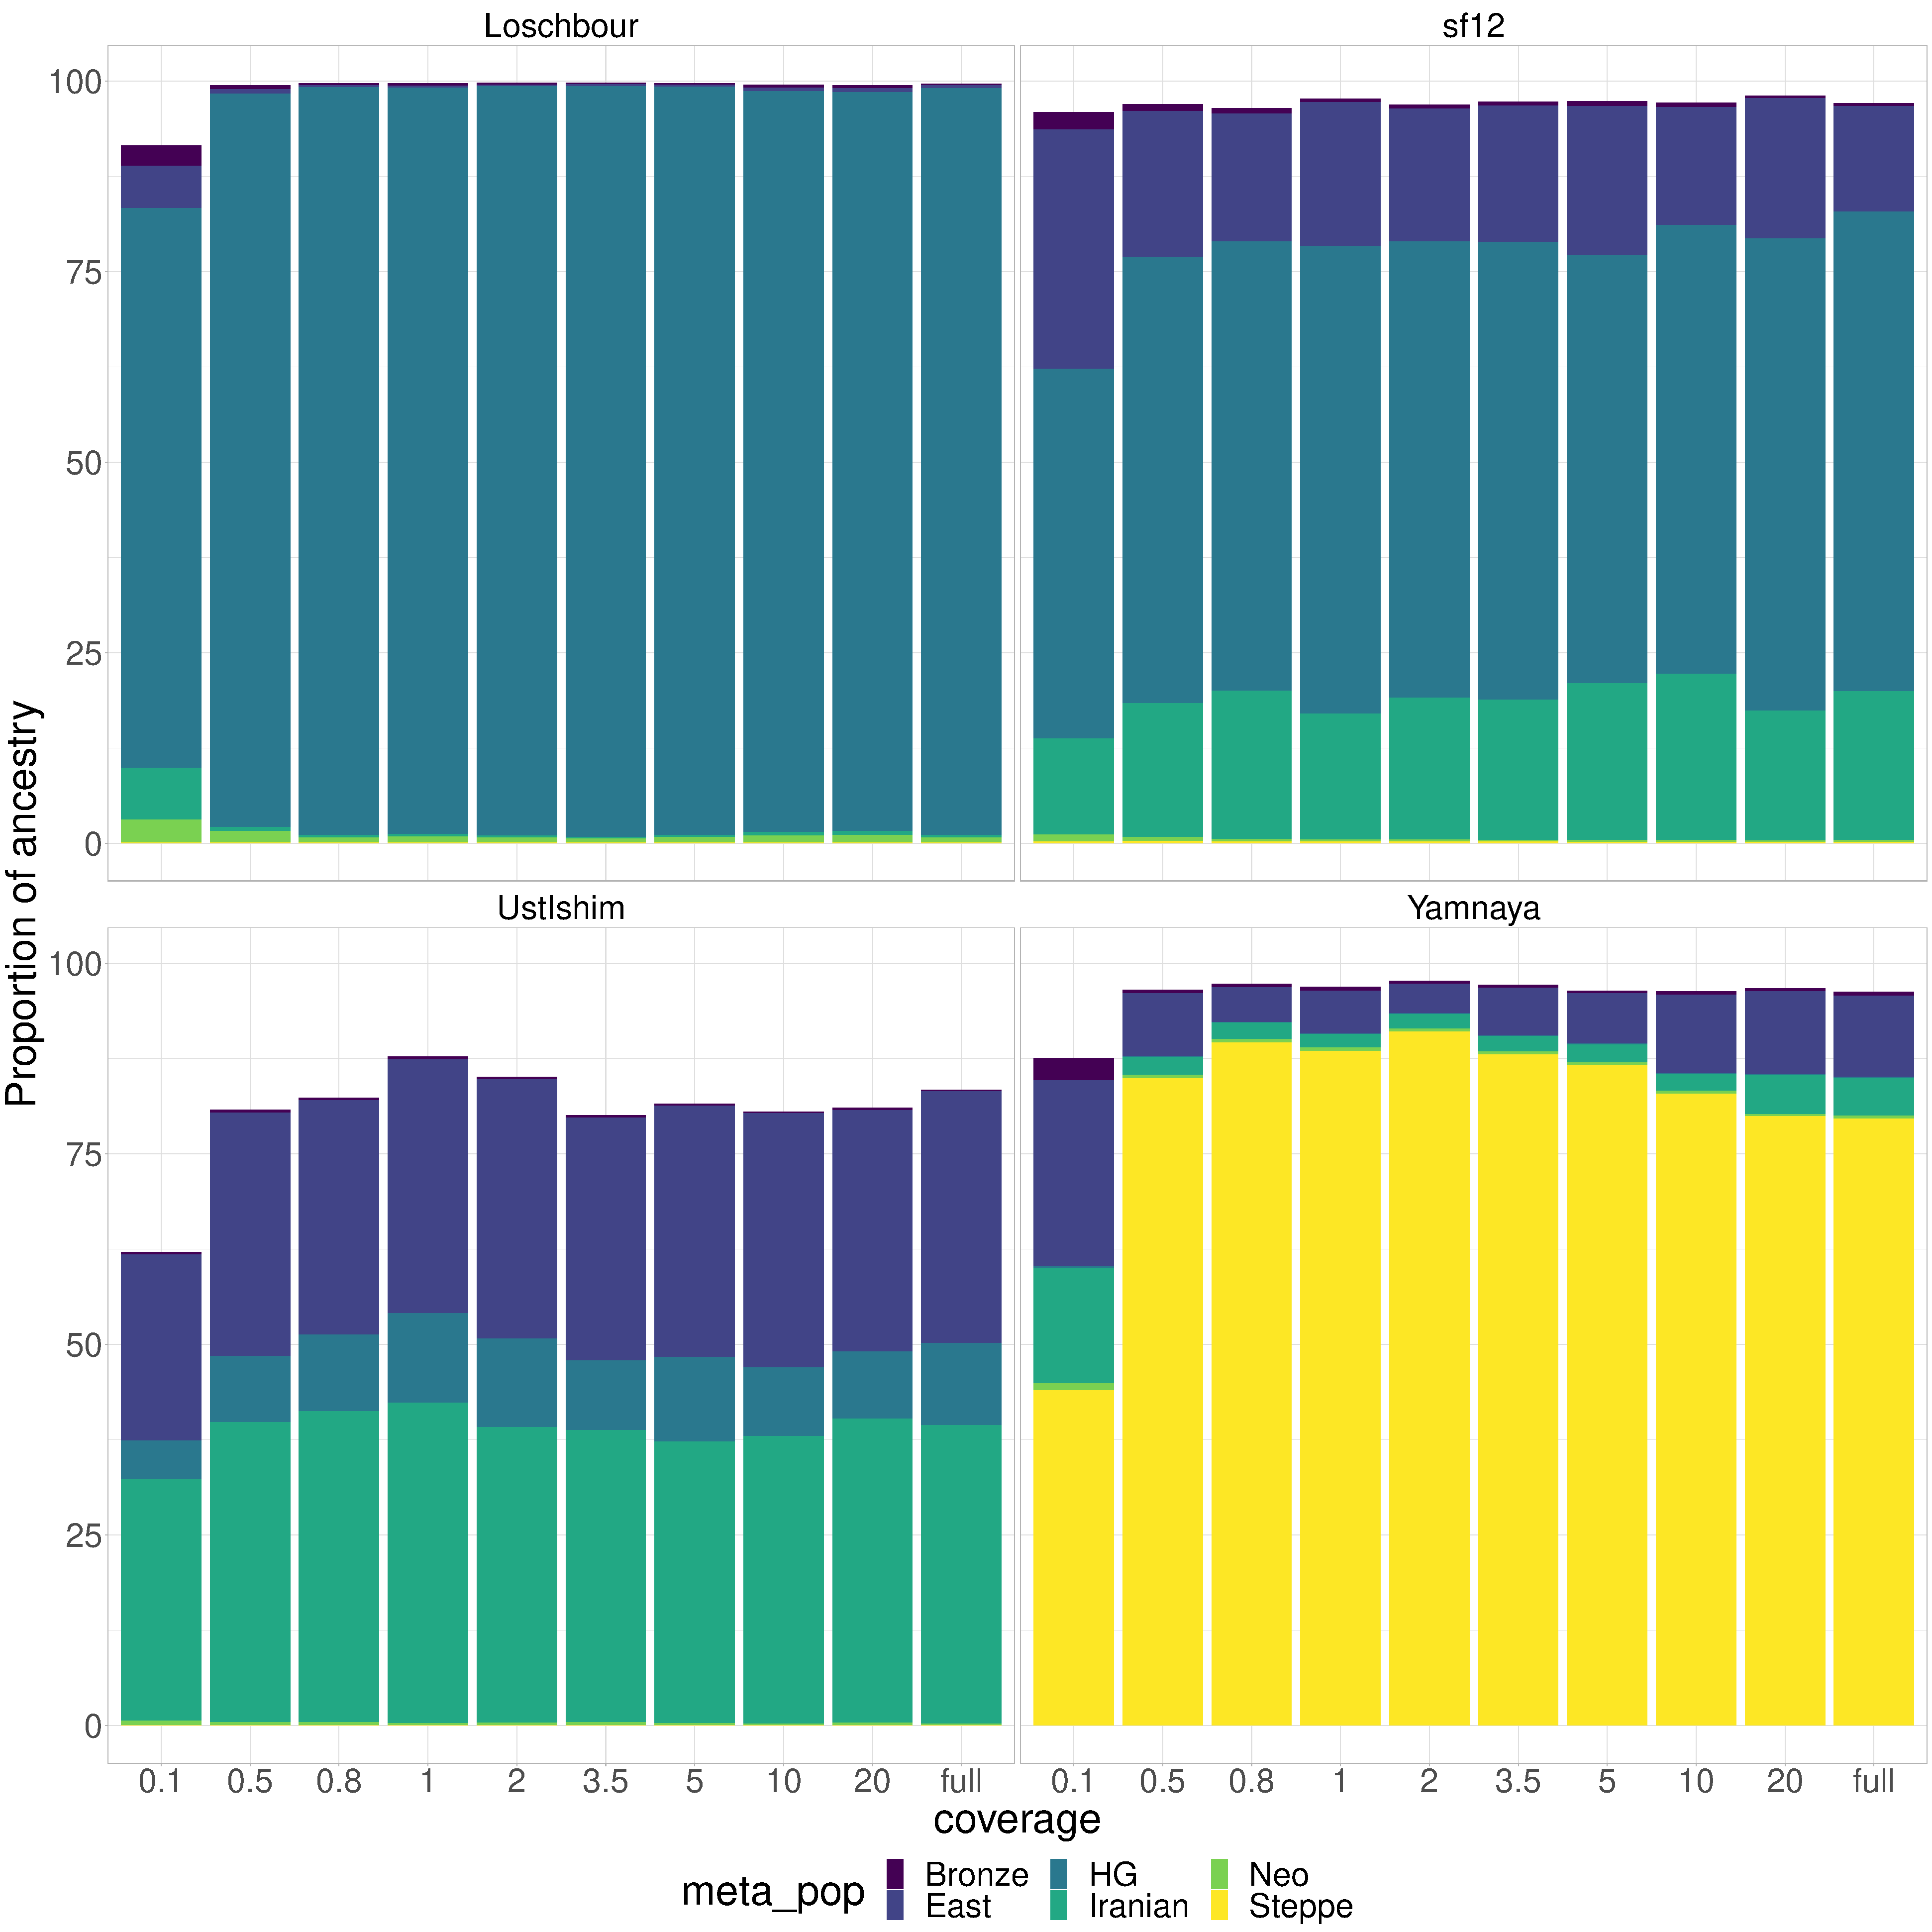
\includegraphics[width=1.0\textwidth]{../images/chapter1/Allpops_SF_downsampled.pdf}
    \caption{Each panel gives information for a different downsampled genome. Bars represent proportion of ancestry inferred by SOURCEFIND, coloured by different surrogates. Different coverages for the same individual are given within each panel. All 39 ancient surrogates were used. Only surrogates with more than 5\% are shown. Ancient surrogates grouped into hand-assigned `meta-populations' for visual clarity. LBK excluded because of anomalously poor results.}
    \label{fig:SOURCEFIND_AllPSop_downsampled}
\end{figure}

Again, Loschbour seems to be the least affected by coverage, with only slight differences between the 0.5x and full coverage samples. It is known that Upper Palaeolithic / Early Neolithic Hunter-Gatherer populations were small and lacked genetic diversity \cite{excoffier1999hunter, Lazaridis2014, Fu2016}. It is therefore expected that Hunter-Gatherers would share longer IBD segments than individuals from outbred populations. Accordingly, this may make estimating SOURCEFIND proportions easier.


\section{Issues and possible solutions for low coverage ancient DNA}

The previous section outlined a drawback of performing ChromoPainter analysis on low coverage ($<$0.5x) ancient DNA samples; low coverage samples appear to be shifted towards the origin of a principle component analysis (PCA) relative to the same sample at higher coverage (Fig. \ref{fig:PCA_panel_allInds_allCoverage}) and can contain ancestry estimates that are not present in the same full coverage sample (Fig. \ref{fig:3pop_SF_downsampled}).  This is evident for the lowest coverage samples at 0.1x and suggests that samples of this coverage cannot be reliably analysed using         current methodology.

In order to solve the issue of coverage-related bias, it is first necessary to determine at which stage of the analysis pipeline the bias is introduced. By `analysis pipeline', I refer to the three stages of (1) variant calling, (2) imputation and phasing, and (3) ChromoPainter described in the methods section.

\subsection{PCA imputation test} \label{sec:PCAImputationTest}

To explicitly test at what stage the bias is introduced, I performed a set of principle component analyses on the downsampled data. First, I performed PCA projections of all downsampled ancient individuals onto a set of present-day European individuals (shown in Table \ref{tab:HB_pops}) using i) pre-GLIMPSE genotypes and ii) post-GLIMPSE (imputed) genotypes (Fig. \ref{fig:pre_GLIMPSE_PCA}). PCA projections are used when the target dataset, in this case downsampled ancients, contain variable levels of missing data.  

The results show that there is no apparent coverage-related bias in the pre-GLIMPSE PCA; the 0.1x samples do not substantially differ in their position from the other downsamples of the same individual. However, there is a degree of noise; for example, the LBK downsamples are spread over a small region on the PCA. Here, noise is variability in the position of technical replicates (full coverage samples and their downsamples) on the PCA. 

On the other hand, downsamples of UstIshim, sf12 and Loschbour are shifted to the centre of the post-GLIMPSE PCA and away from the full coverage individual and other downsamples. This suggests that coverage-related bias is being introduced in the imputation stage. At the same time, GLIMPSE appears to have removed some of the noise in the downsampled individuals of coverage $\geq$0.5x. For instance, the noise observed in the LBK samples in the pre-imputation PCA is substantially reduced and the samples cluster more tightly.  

I also performed PCAs based upon an all-v-all ChromoPainter painting using the same set of present-day European samples (Table \ref{tab:HB_pops}) and downsampled ancient individuals as previously, in both linked and unlinked modes. There is an increased amount of noise and evidence of coverage-related bias relative to the post-GLIMPSE genotype PCA. Fig. \ref{fig:CP_linked_unlinked}) displays the PCA for the same painting, but using the unlinked chunkcounts matrix. Comparing the linked and unlinked PCAs shows the effect of including linkage (i.e. haplotype information) on the amount of bias and noise across each sample. Per-sample, there appears to be reduced noise in the unlinked painting.

These results suggest that imputation using GLIMPSE introduces a degree of bias into 0.1x samples that is not apparent on non-imputed genotypes. They also suggest that ChromoPainter introduces an additional degree of bias when analysing haplotypes, or that it amplifies bias already present introduced at the imputation stage. Accordingly, removing SNPs which have been poorly imputed may be a way to mitigate such biases. An alternative explanation may be that an increase in switch-errors may be driving the signal, as it has been previously shown that phasing accuracy declines with coverage \cite{delaneau2018integrative}.

\begin{figure}[htp]
    \centering
    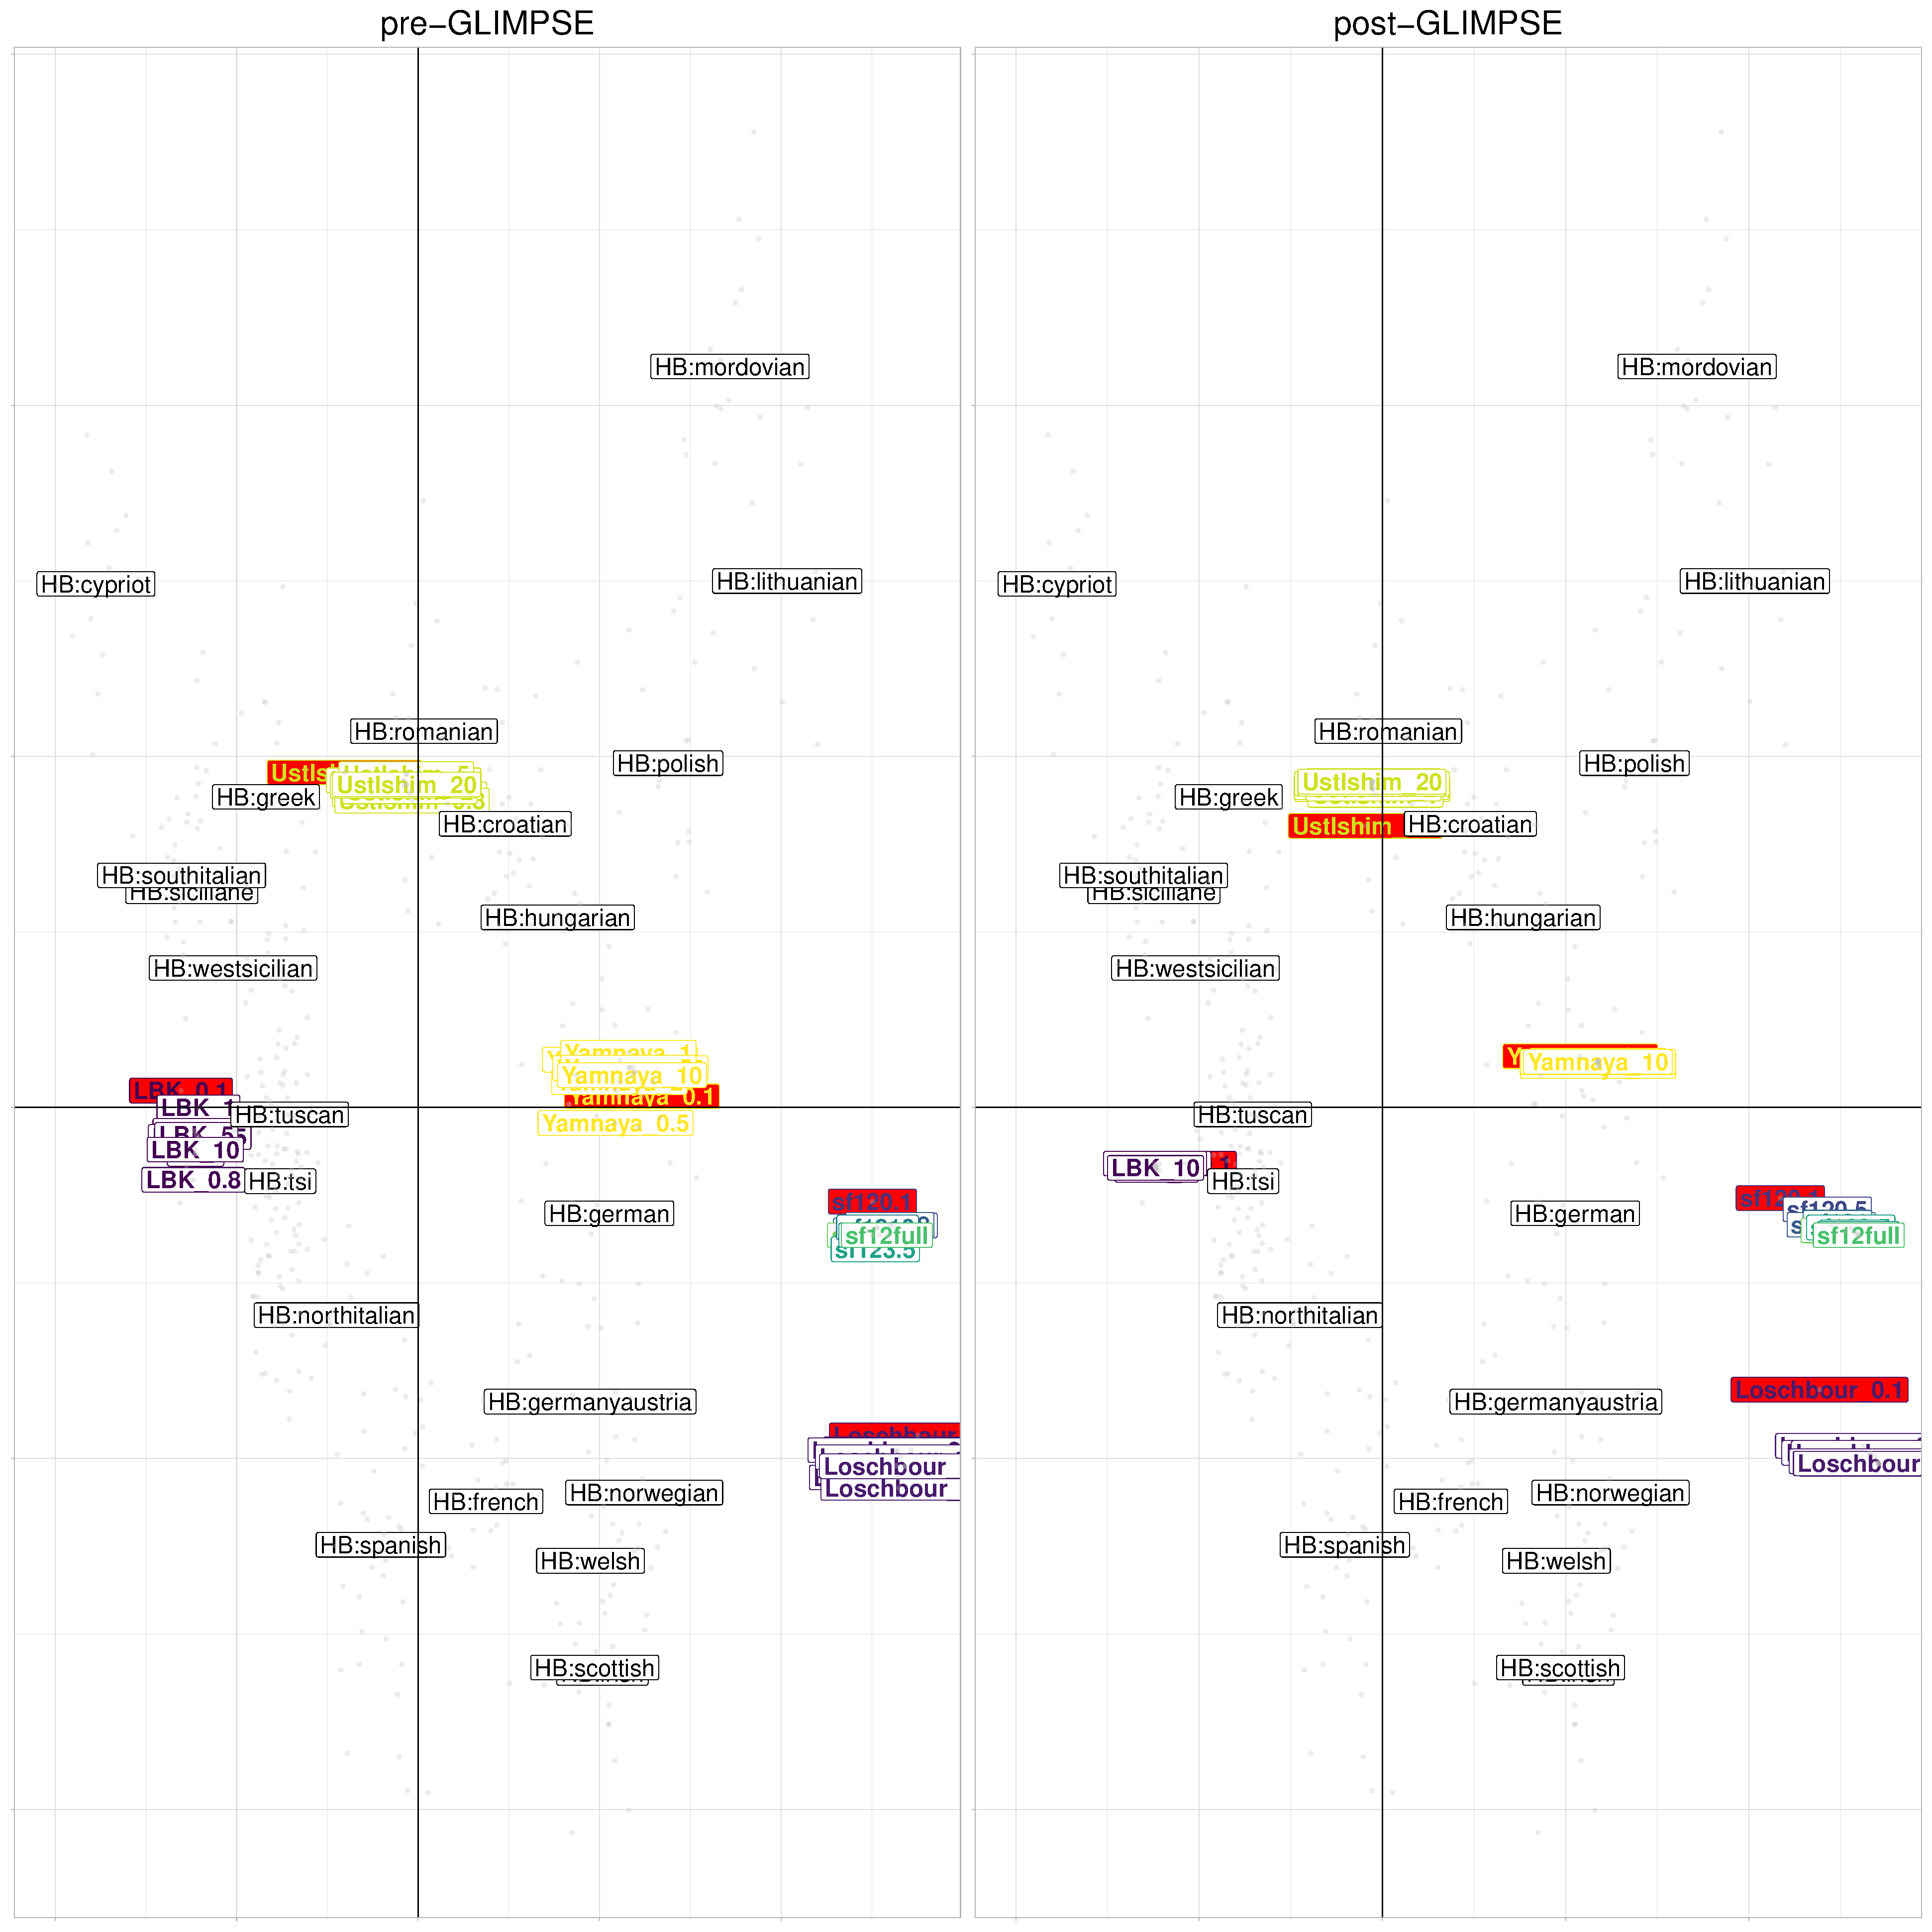
\includegraphics[width=1.0\textwidth]{../images/chapter1/pre_post_GLIMPSE_PCA.pdf}
    \caption{Principle Component Analysis. Left - pre-GLIMPSE genotypes. Right - post-GLIMPSE (imputed) genotypes. White labels correspond to the midpoint of all samples from that population, grey points correspond to modern individuals. 0.1x samples highlighted in red for clarity. Black lines are $y=0; x=0$.}
    \label{fig:pre_GLIMPSE_PCA}
\end{figure}

\begin{figure}[htp]
    \centering
    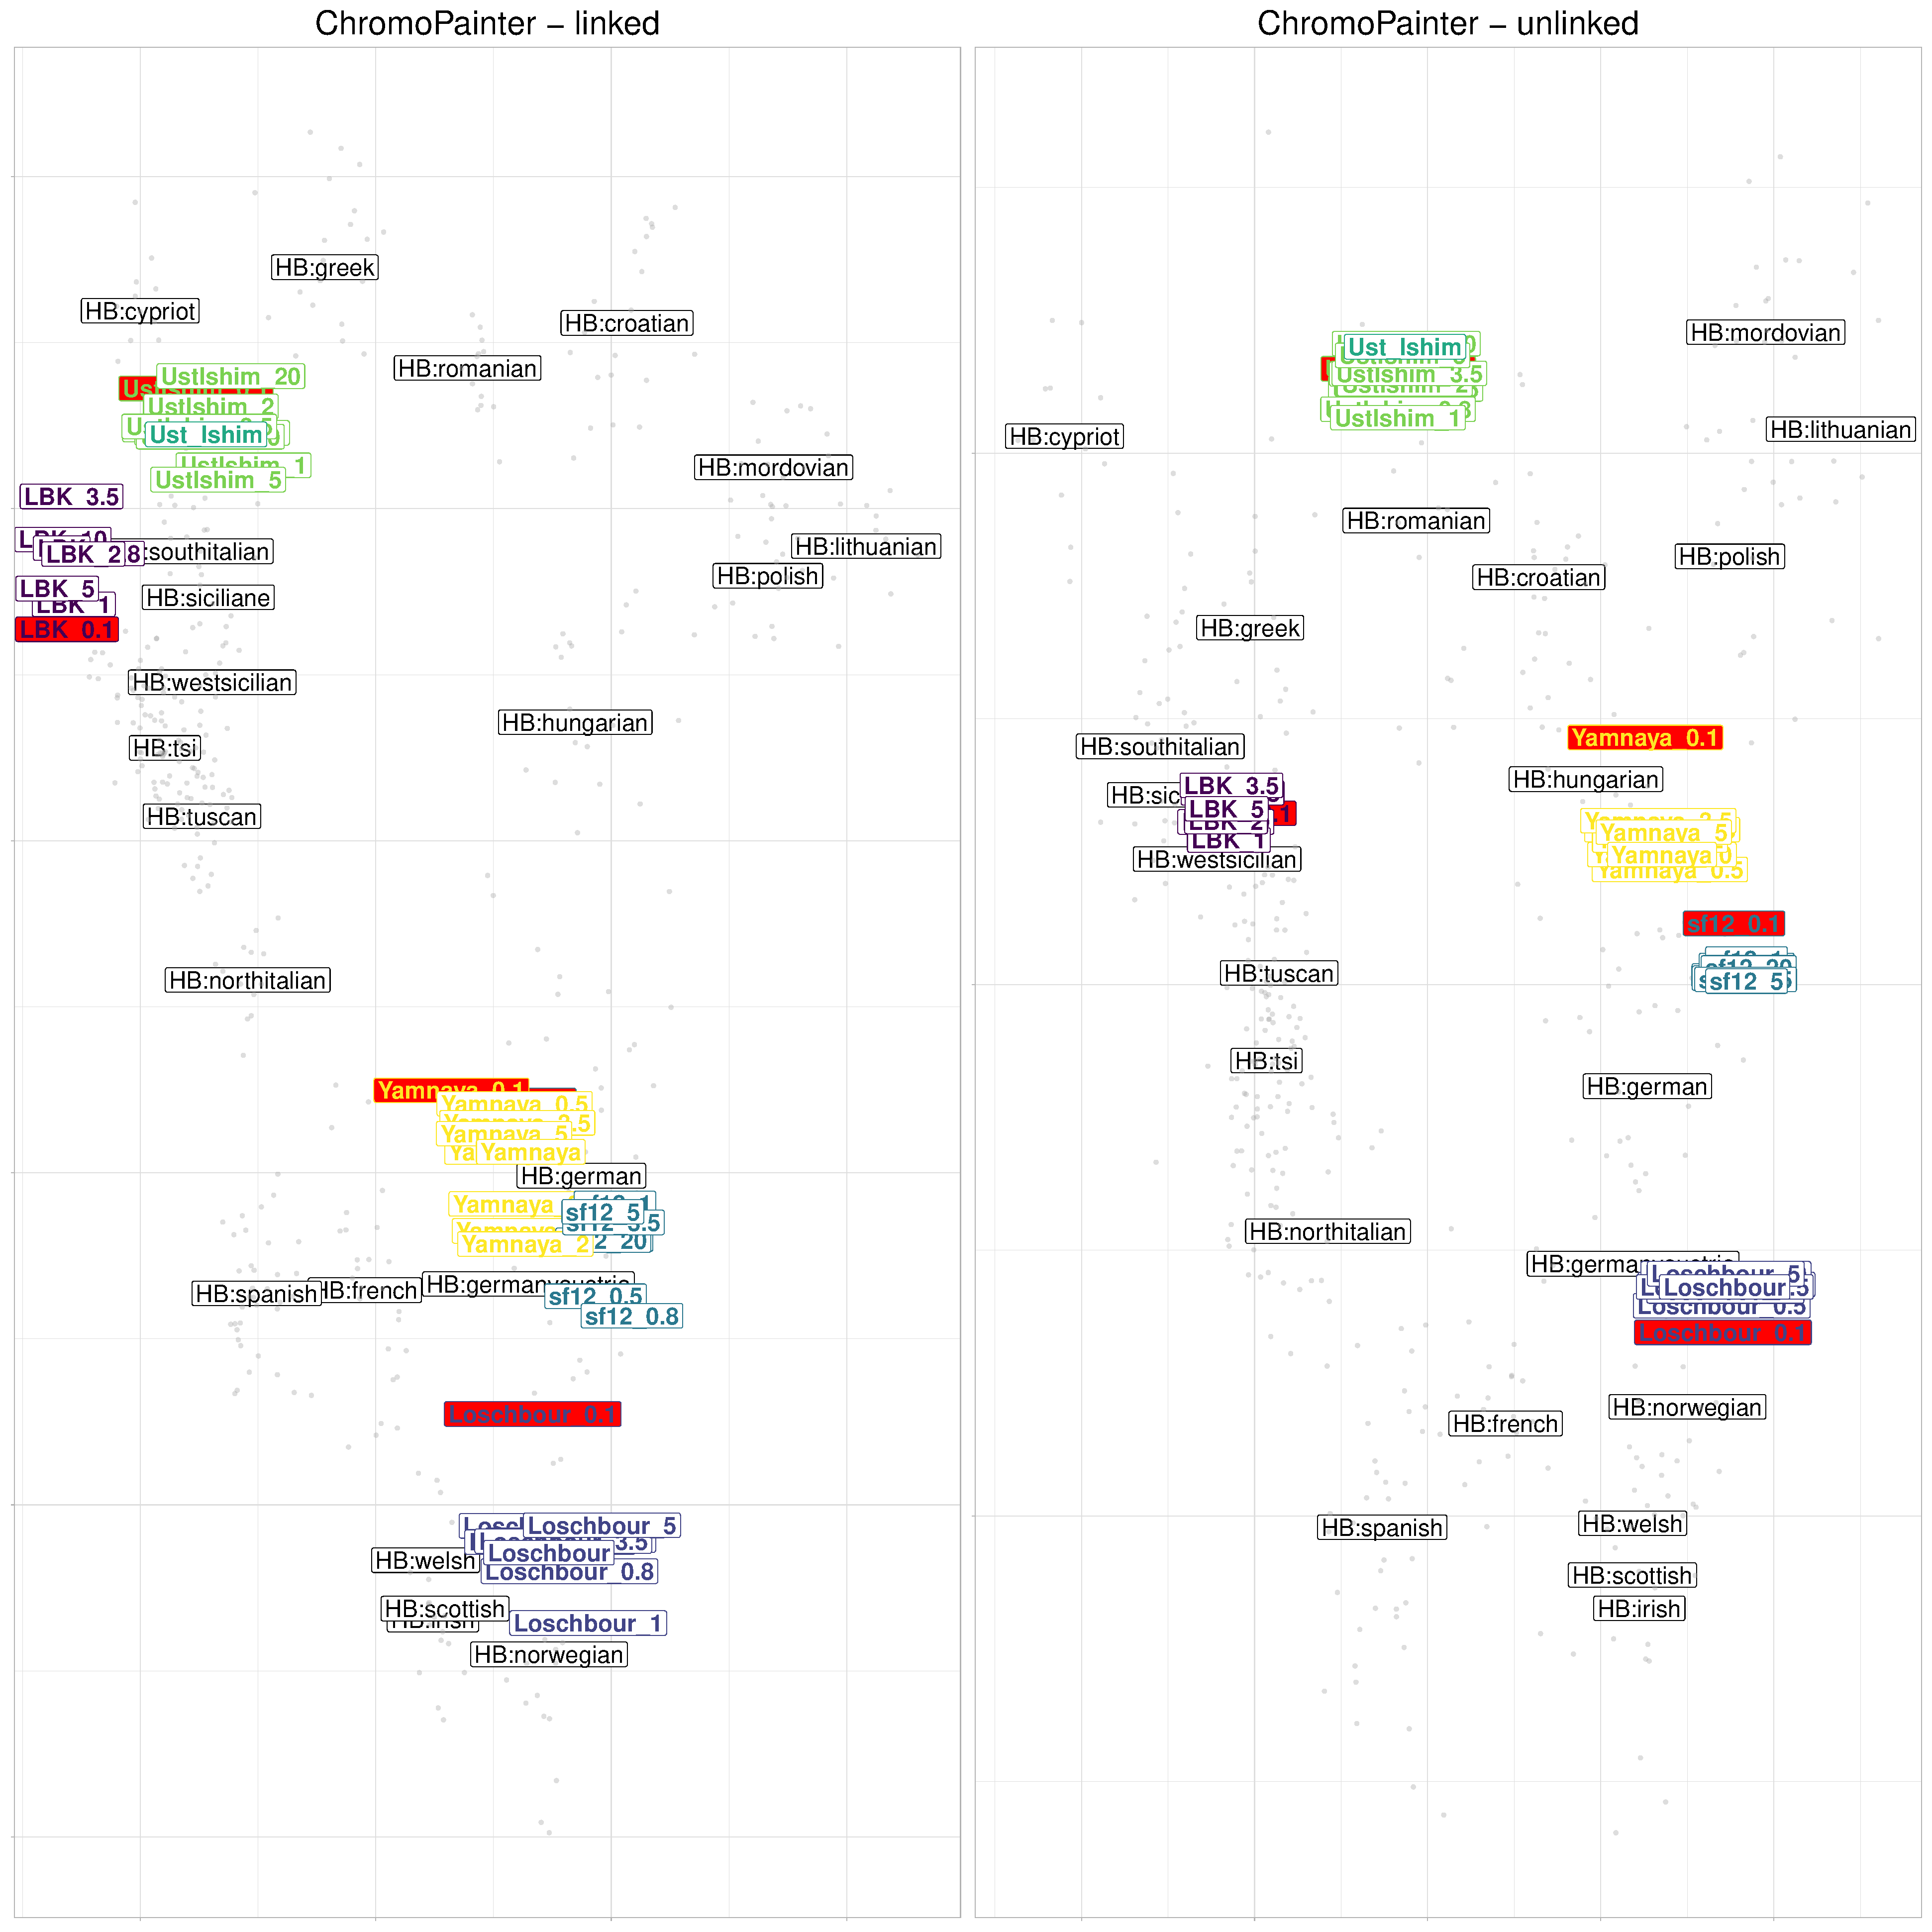
\includegraphics[width=1.0\textwidth]{../images/chapter1/CP_linked_unlinked.pdf}
    \caption{Left - ChromoPainter Linked. Right - ChromoPainter Unlinked. White labels correspond to the midpoint of all samples from that population, grey points correspond to modern individuals. 0.1x samples highlighted in red for clarity. Black lines are $y=0; x=0$.}
    \label{fig:CP_linked_unlinked}
\end{figure}

\subsection{Direct imputation test} \label{DirectImputationTest}

The previous section suggested that imputation plays a role in the introduction of coverage-related bias. However, it is not clear whether it is `bias', i.e.\ towards the reference population used to assist imputation, or `noise' due to random incorrect imputation. To directly test whether the effect of imputation is noise or bias, I used the Human Origins dataset (described in Appendix section \ref{HumanOriginsAppendix}), containing the genotypes of 5998 present-day individuals from across the world at 560,442 SNPs. I chose to use present-day samples because there is a larger total number of individuals and larger number of individuals per population, giving more power to detect any potential bias. Additionally, the populations in present-day samples are more homogenous and well-defined compared to ancient groups. I set all but 70,000 random SNPs as missing and imputed missing positions using the HRC as a reference, in order to simulate a dataset where the majority of SNPs are imputed. I then performed an all-v-all painting of i) the original Human Origins dataset where none of the 560,442 SNPs had been imputed and ii) the simulated dataset where 430,000 SNPs had been imputed. 

Bias occurs when missing genotypes are incorrectly imputed with variants from certain populations more frequently than others. We might expect these populations to be those which are more prevalent in the reference panel. We would correspondingly expect bias to mean that, when painted, some donor populations would donate more than others, relative to if no imputation had taken place. On the other hand, if `noise' is dominating results, we would expect the incorrectly imputed genotypes to be randomly distributed across populations, and similarly we would not expect to see any populations donating more than others relative to if no imputation had taken place. 

Therefore, we can compare the amount different donor groups donate under the dataset where none of the 560,442 SNPs had been imputed versus the dataset where 430,000 (86\%) of these SNPs have been imputed by plotting the mean amount donated by each population using imputed SNPs and non-imputed SNPs (Fig. \ref{fig:imputed_nonimputed_donation}). The 20 populations that contribute most are a set containing European / Ashkenazi Jewish / Levite Jewish populations. Notably, the Haplotype Reference Consortium panel that was used to impute the data consists primarily of individuals of European descent. The two populations which are over-copied the most after imputation are two English populations from Kent and Cornwall. This suggests that there is a most likely a bias towards copying more from European populations when the data has been imputed using the HRC. 

Another consideration is the concept of reference \textit{sequence} bias, where genotypes are imputed  with a higher accuracy when they contain more reference alleles. To display this effect, I calculated the proportion of correctly imputed genotypes in 0.1x and 0.5x downsamples and stratified by genotype class (Table \ref{tab:genotype_class_prop}). In the case of 0.5x downsamples, adding reference alleles to the genotype increased the accuracy of imputation. For 0.1x downsamples, reference homozgyous genotypes were imputed more accurately than non-reference homozygous genotypes. In 0.1x downsamples, non-reference homozygous genotypes were imputed approximately as accurately as heterozygous genotypes, potentially in part because of the difficult of calling heterozygous genotypes in very low coverage samples.

\begin{table}
\centering\begingroup\fontsize{10}{10}\selectfont

\begin{tabular}[t]{lccc}
\toprule
type & prop correct 0.1x & prop correct 0.5x & Number of SNPs\\
\midrule
1/1 & 0.880 & 0.967 & 476,046\\
0/1 & 0.850 & 0.971 & 662,819\\
0/0 & 0.954 & 0.989 & 1,003,260\\
\bottomrule
\end{tabular}
\caption{Aggregated proportion of genotypes in 0.1x and 0.5x across downsamples which match the genotype in the equivalent full coverage individual, stratified by whether genotype in full coverage sample is heterozygous, homozygous reference or homozygous alternative. Number of SNPs is the total number of SNPs aggregated across all downsamples.}
\endgroup{}
\label{tab:genotype_class_prop}
\end{table}




\begin{figure}[htp]
    \centering
    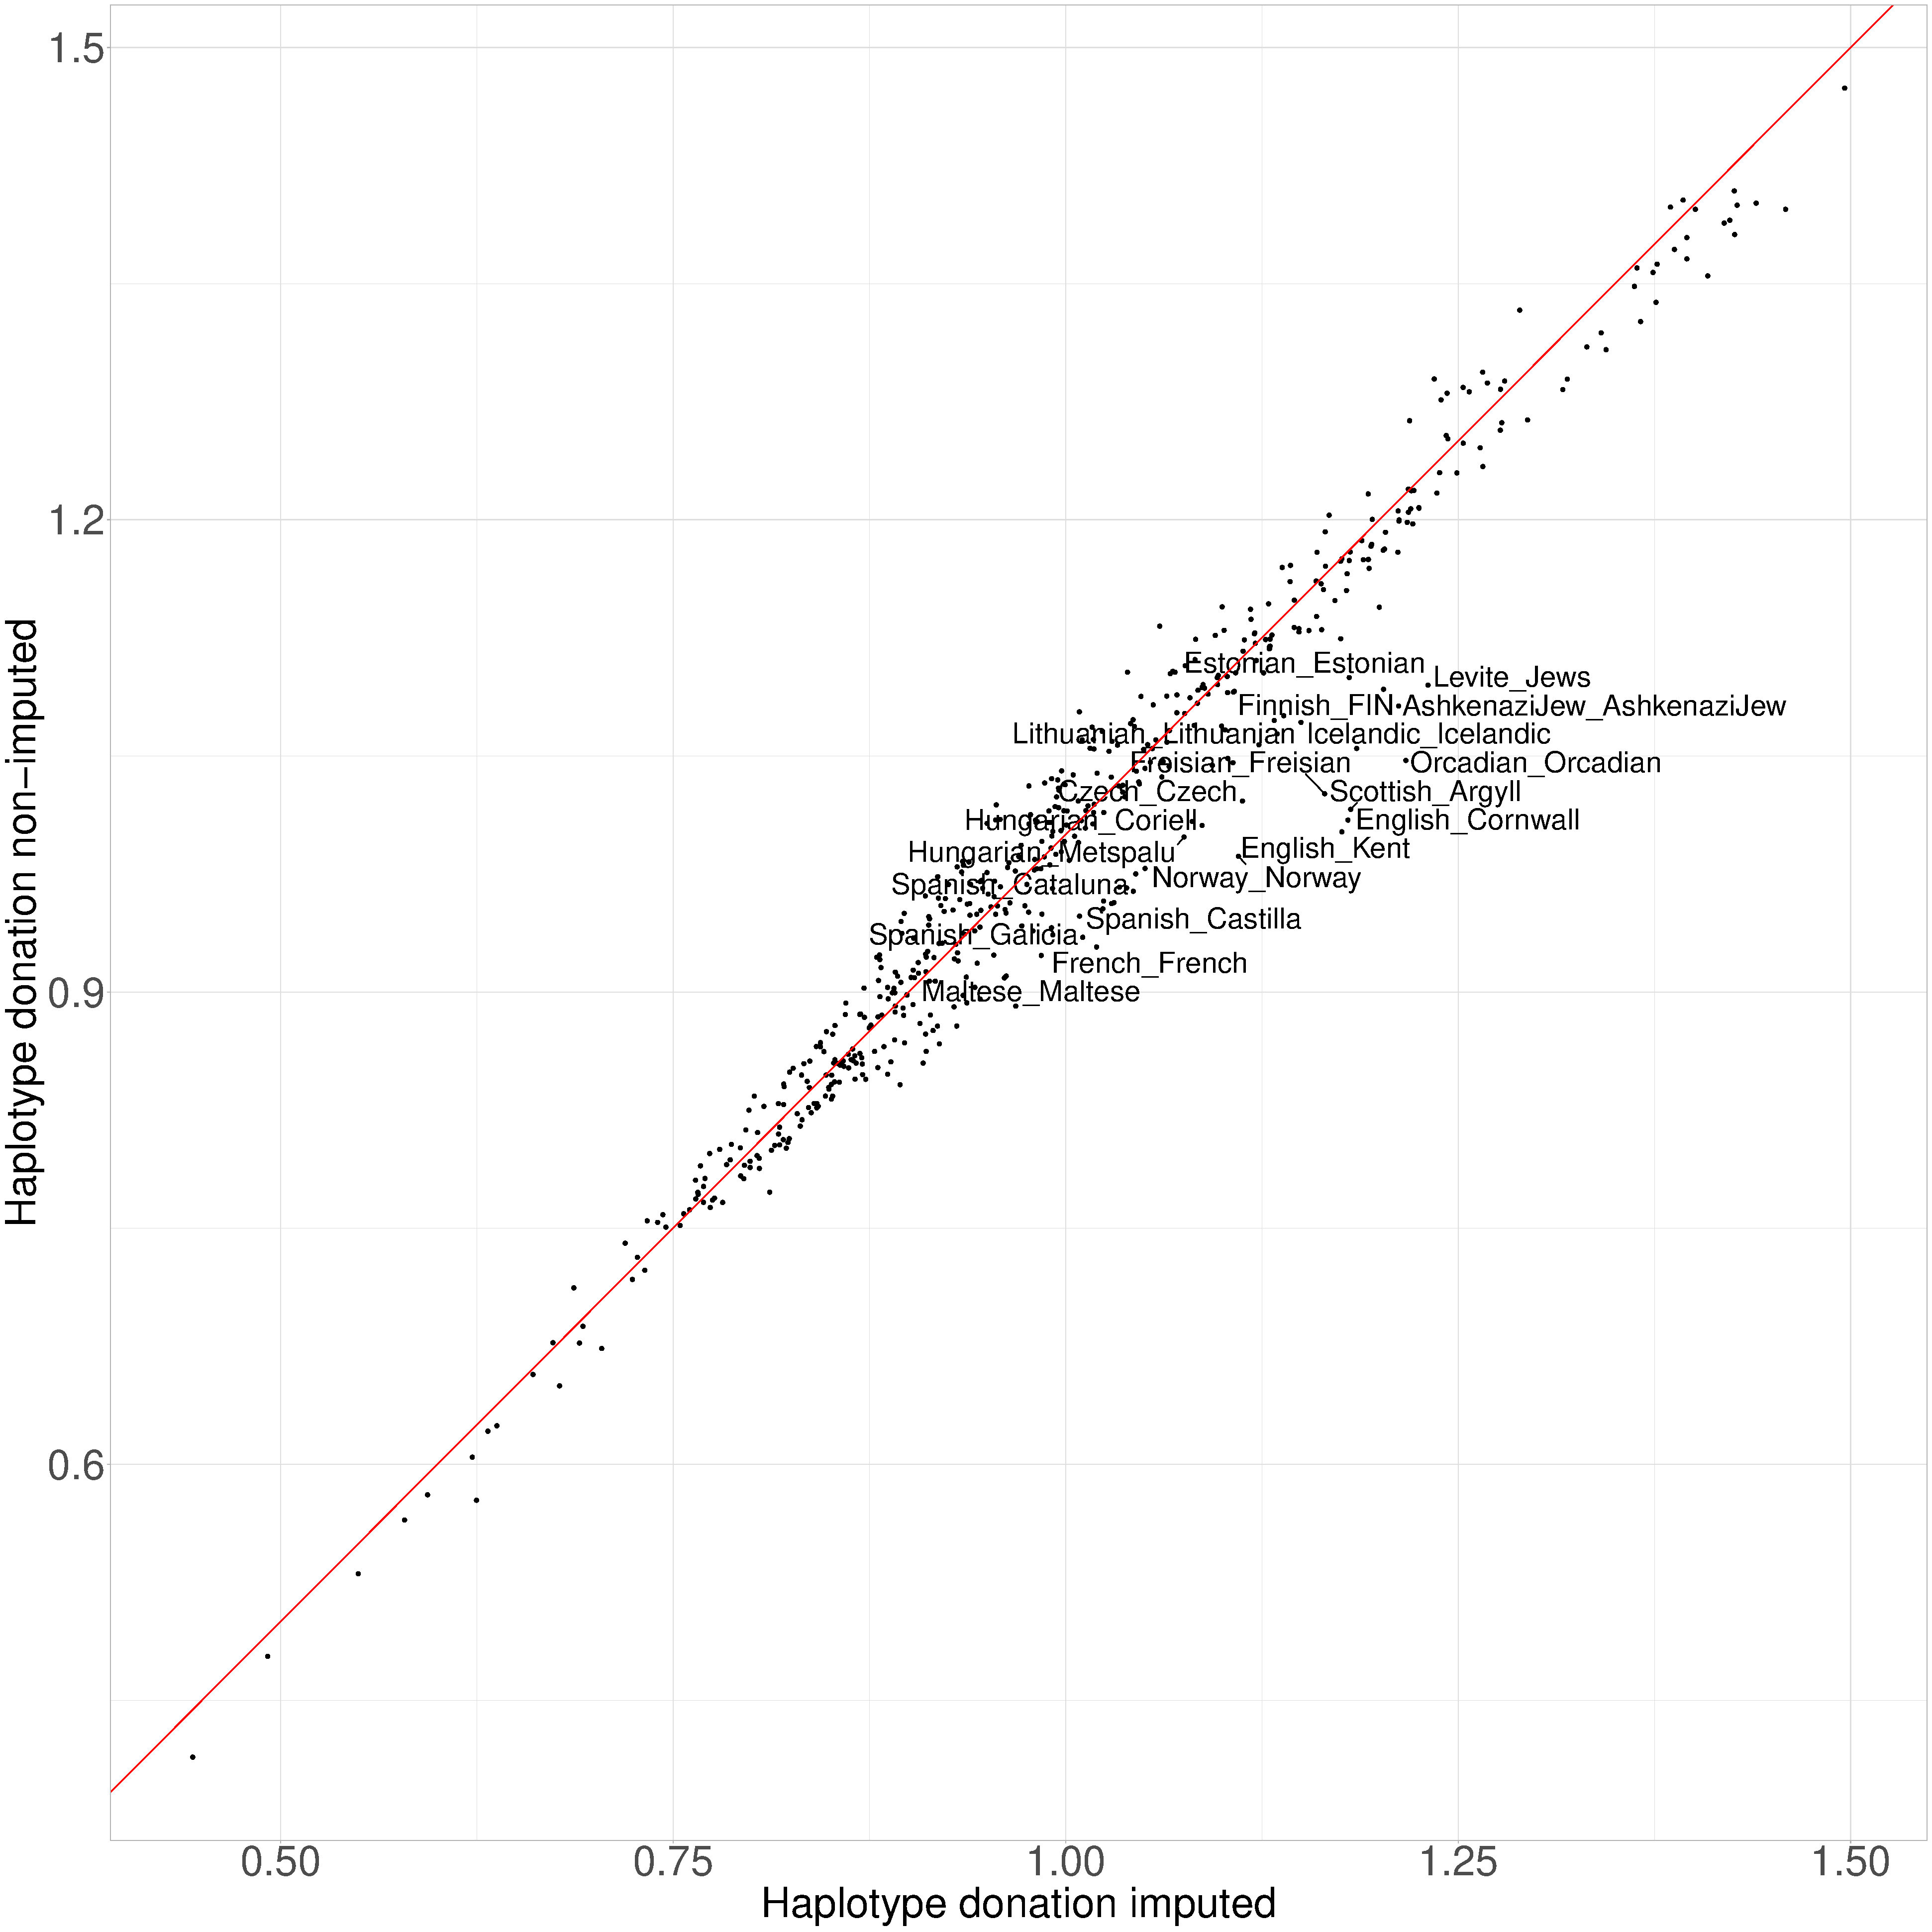
\includegraphics[width=1.0\textwidth]{../images/chapter1/donation_imputed_nonimputed.pdf}
    \caption{Comparison of the mean normalised cM donated by each donor population using the imputed and non-imputed SNP sets. The 20 populations with the largest difference between imputed and non-imputed donation are highlighted. Red line is line of $y=x$.}
    \label{fig:imputed_nonimputed_donation}
\end{figure}

\section{Solutions} \label{sec:Solutions}

In this section I will explore potential solutions to the issue of coverage-related bias. Based on the findings in previous sections, imputation causes bias towards particular reference populations in modern samples.  

\subsection{Accounting for allele likelihoods}

Section \ref{sec:DescriptionChromoPainterV2Uncertainty} describes an improvement to the ChromoPainter algorithm. Instead of assuming that each allele on a haplotype is correct with a probability $1-\theta$, where $\theta$ represents an error probability, the posterior genotype probability from GLIMPSE is accounted for in the emission probabilities of the copying model. The motivation behind this update is that the uncertainty associated with genotype calls at low coverage is suitably propagated throughout the painting process, resulting in uncertain alleles contributing less towards the expected copying values than more certain ones. This is similar in spirit to that of Viera et al (2016), who account for genotype likelihoods to infer inbreeding IBD tracts from low coverage sequencing data \cite{vieira2016estimating}.

To determine whether accounting for allele likelihoods improved the painting accuracy of a low-coverage genome, I painted the individuals downsampled to 0.1x and 0.5x and corresponding full coverage samples using the `standard set' of ancient reference individuals, using both ChromoPainterV2 and ChromoPainterV2Uncertainty. I then calculated Pearson's correlation between the copyvectors of full coverage and downsampled individuals using the two different methods (Fig. \ref{fig:uncertainty_v_noUncertainty_0.5x_0.1x}). This shows that at 0.1x, the ChromoPainterV2 method clearly outperforms ChromoPainterV2Uncertainty across all samples, whereas at 0.5x, the new method marginally outperforms the standard method. Therefore, while accounting for allele likelihoods may improve performance in cases of coverage $\geq$0.5x, which has been shown to still capture some haplotype information, it does not help in cases of coverage of 0.1x where bias problems persist.


\begin{figure}[htp]
    \centering
    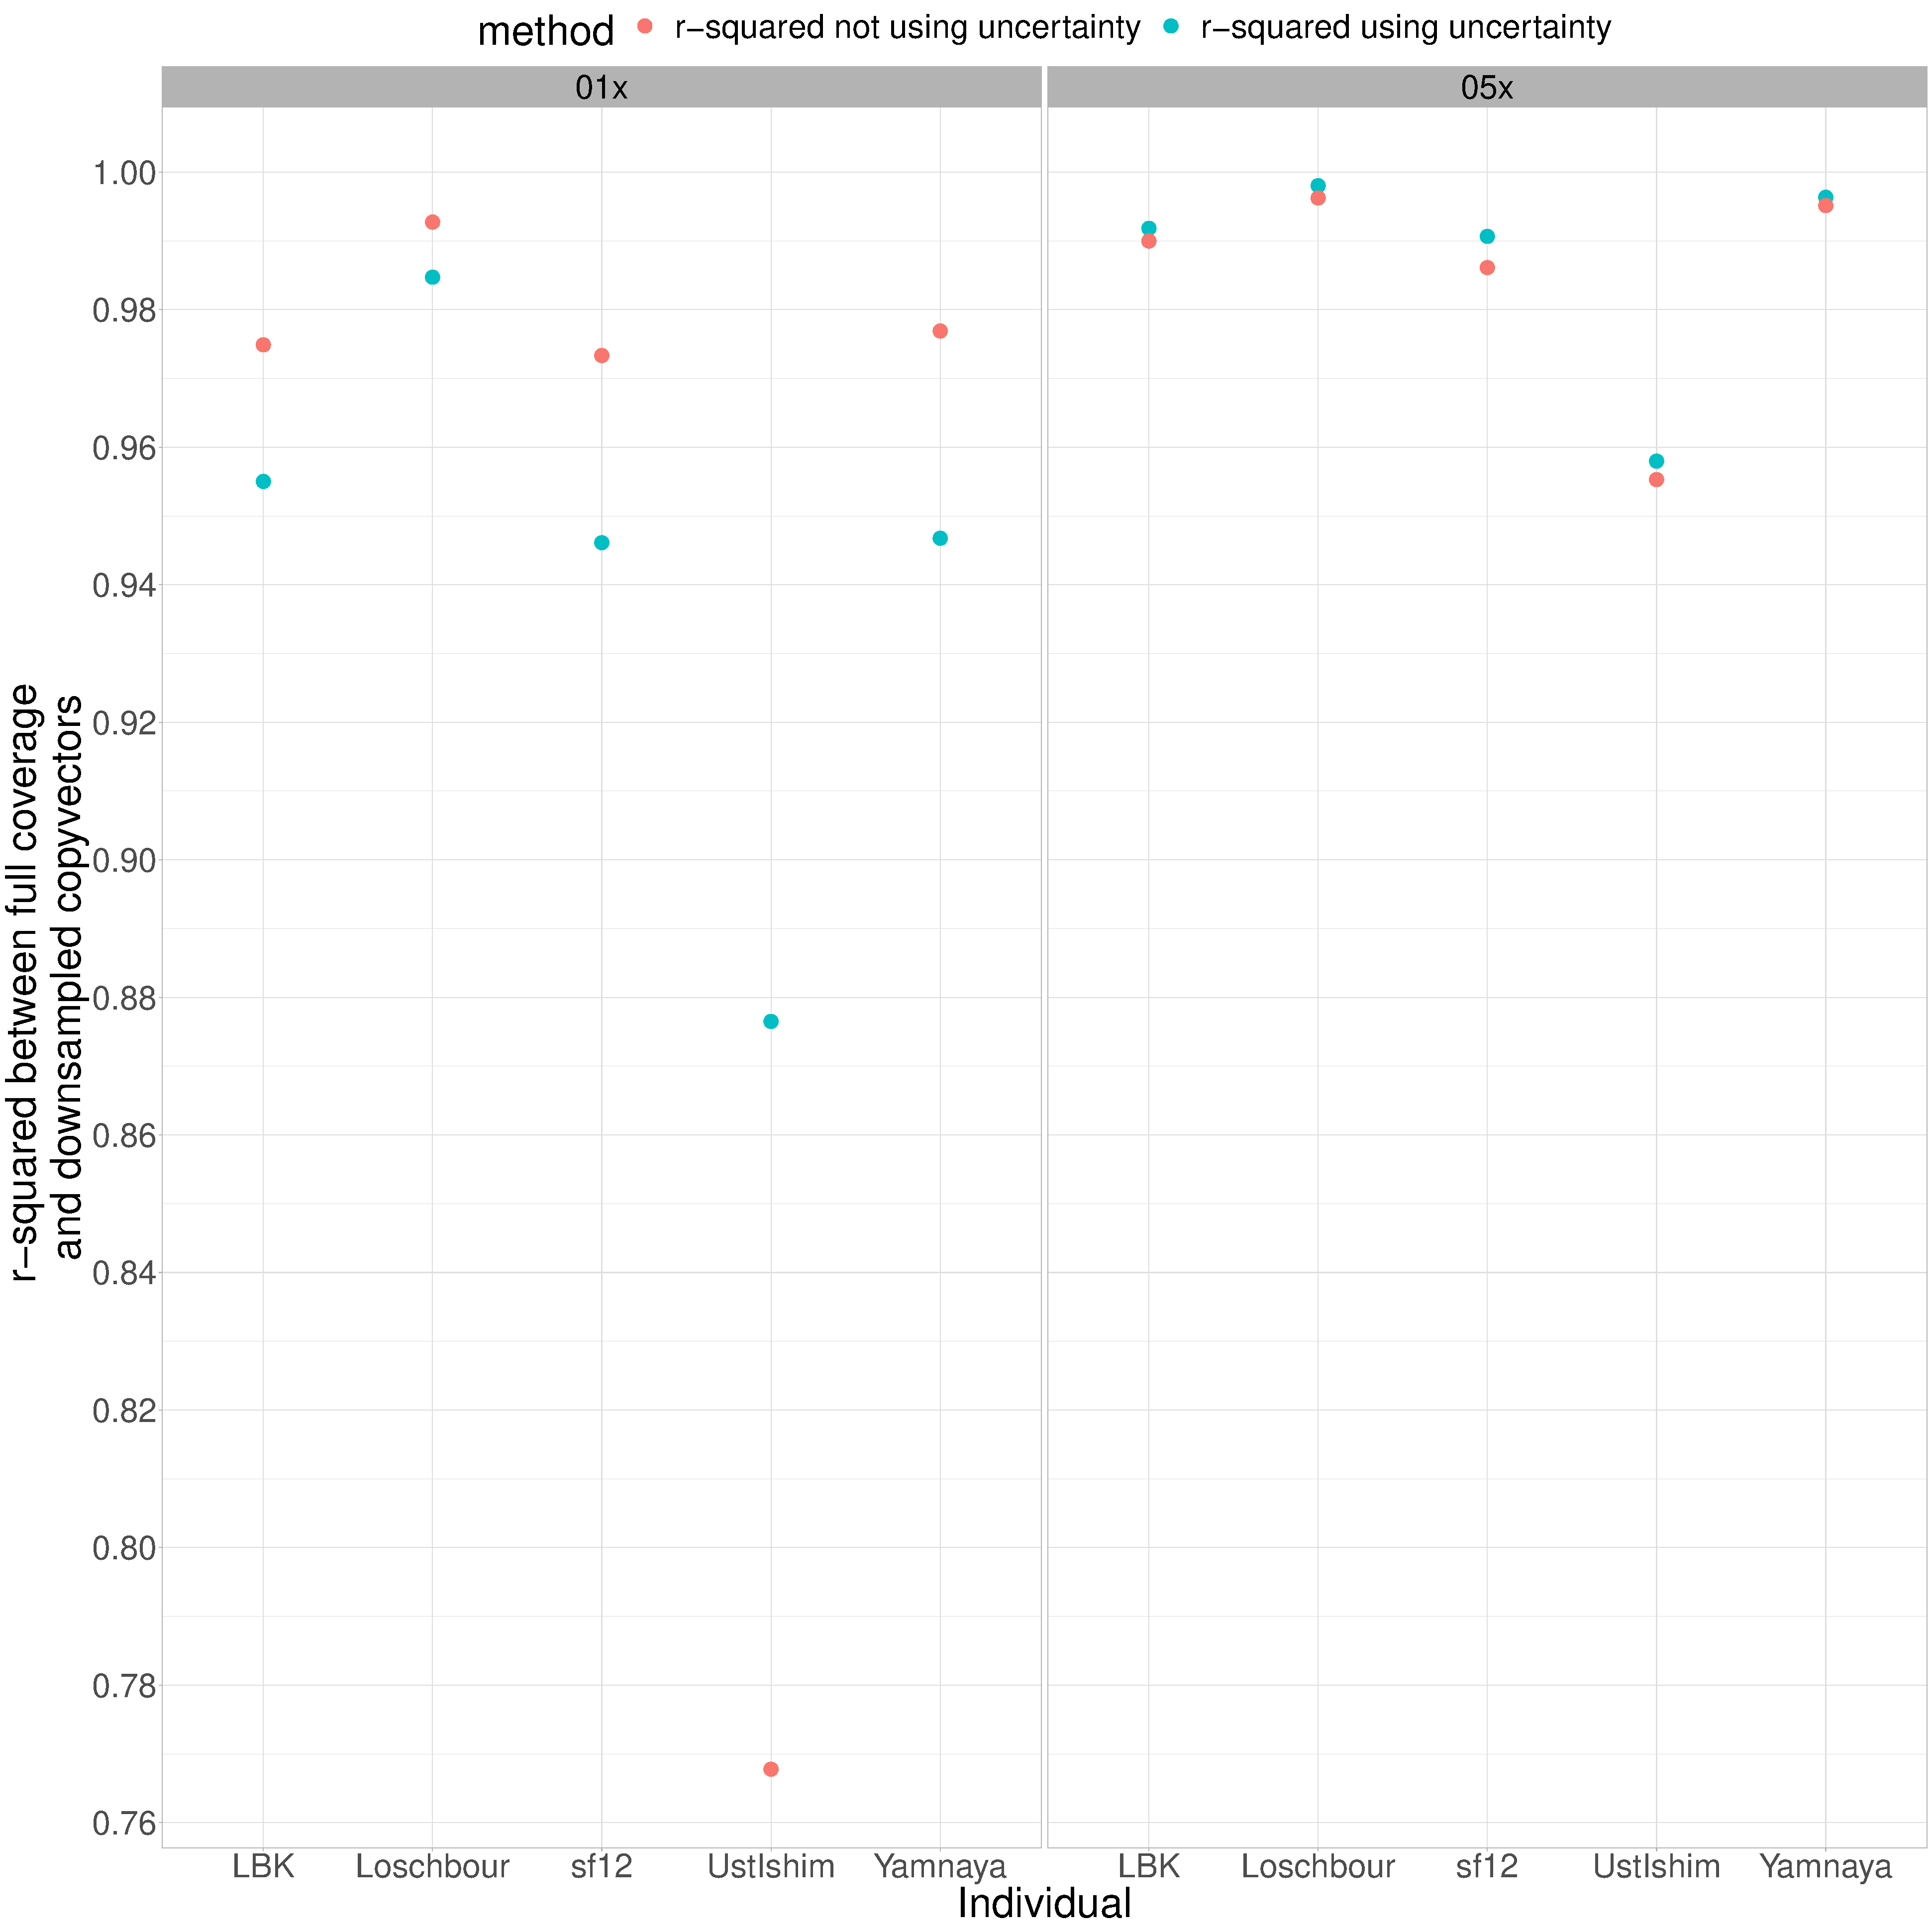
\includegraphics[width=1.0\textwidth]{../images/chapter1/uncertainty_v_noUncertainty_0.5x_0.1x.pdf}
    \caption{Comparison of performance of ChromoPainterV2 and ChromoPainterV2Uncertainty. Panels correspond to samples downsampled to 0.1x (left) and 0.5x (right). Points correspond to the r-squared between the downsampled individual and the same individual at full coverage. Red points are values obtained from ChromoPainterV2 and blue points are those obtained from ChromoPainterV2Uncertainty.}
    \label{fig:uncertainty_v_noUncertainty_0.5x_0.1x}
\end{figure}


\subsection{Filtering SNPs}

In this section, I will test whether filtering the set of input SNPs on different criteria reduces the effect of coverage related bias. 

The frequency of a particular variant in the reference panel (RAF - minor reference allele frequency) used for imputation is known to affect how accurately that variant can be imputed \cite{rubinacci2021efficient, delaneau2018integrative, Browning2016, hui2020evaluating}. Specifically, we expect variants which are less frequent in the reference panel to be imputed at a lower accuracy than those which are more frequent. Therefore, removing variants with a low frequency in the reference panel may mitigate the coverage related bias by removing variants which have been incorrectly imputed. In other words, we want to retain the SNPs where both alleles are relatively common within the population. 

For each individual, I took the 428,425 SNPs in the HellBus set and removed SNPs with $0.1 > RAF$ or $RAF > 0.9$, removing an average of 50,187 SNPs per individual. $RAF$ refers to the frequency of the allele in the 1000 genomes reference panel used to phase and impute the HellBus dataset. I then painted individuals downsampled to 0.1x and 0.5x using the standard set of 125 ancient donor individuals.  

Comparing the $TVD$ values between the copvyectors showed that, whilst there was a marginal improvement at 0.1x, this did not improve the 0.5x copyvectors (Table \ref{tab:TVD_table}). 

I then chose to filter SNPs based on $max(GP)$ at each position. $max(GP)$ correspond to the accuracy with which a SNP has been imputed, with higher values reflecting a higher chance of that genotype being imputed correctly. For each individual downsampled to 0.5x and 0.1x, I only retained positions where the $max(GP) >= 0.990$. For the 0.5x individuals, this resulted in a total of 348,852 SNPs for LBK, 339,949 for Loschbour, 315,075 for sf12, 308,961 for UstIshim and 386,484 for Yamnaya. Because different SNPs were removed from different individuals, each individual was painted separately. The same standard set of 124 ancient donors was used. Again, this did not improve the accuracy of the copyvectors. 


\begin{table}
\centering
\begin{tabular}[t]{lrrrrrrrr}
\toprule
sample & u\_01x & s\_01x & r\_01x & gp\_01x & u\_05x & s\_05x & r\_05x & gp\_05x\\
\midrule
LBK & 0.926 & 0.927 & 0.933 & 0.746 & 0.981 & 0.981 & 0.982 & 0.959\\
Loschbour & 0.898 & 0.898 & 0.907 & 0.654 & 0.980 & 0.980 & 0.976 & 0.925\\
sf12 & 0.923 & 0.923 & 0.942 & 0.774 & 0.981 & 0.981 & 0.980 & 0.950\\
UstIshim & 0.944 & 0.944 & 0.945 & 0.827 & 0.980 & 0.980 & 0.976 & 0.960\\
Yamnaya & 0.915 & 0.915 & 0.920 & 0.726 & 0.986 & 0.986 & 0.985 & 0.964\\
\bottomrule
\end{tabular}
\caption{Table of $1-TVD$ values between the copyvectors of full coverage and downsampled individuals. `u' refers to ChromoPainterUncertainty, `s' refers to ChromoPainterV2, `r' refers to filtering SNPs with reference allele frequency (RAF) $0.1 > RAF$ or $RAF > 0.9$ and `gp' refers to filtering by $max(GP) >= 0.990$.}
\label{tab:TVD_table}
\end{table}


\subsection{Restricting analysis to non-imputed SNPs}

Section \ref{sec:PCAImputationTest} showed that imputation was the likely cause of coverage related bias. Thus, restricting ChromoPainter analysis to non-imputed SNPs above a certain coverage may mitigate such bias.

However, removing SNPs may have negative side-effects; increasing the genetic distance between SNPs reduces linkage information and therefore may reduce the overall power to distinguish between closely related haplotypes. At the most extreme case, retaining only a small number of SNPs may effectively reduce the method to unlinked and lose the advantage given by accounting for haplotypes. This may be important if we decide to restrict analysis to non-imputed SNPs, as low coverage samples may only have a small number of high enough coverage, non-imputed SNPs. Therefore, it is important to determine whether samples of a particular coverage have enough regions containing enough high-coverage SNPs to retain the advantages of haplotype-based methods over unlinked ones. 

One case study to test whether a set of SNPs has enough linkage information is to determine whether it is possible to distinguish individuals born in Devon from those born in Cornwall. This has shown to be possible using the fineSTRUCTURE clustering algorithm using linkage information, but not using unlinked methods (ADMIXTURE \cite{alexander2009fast}) \cite{Leslie2015}. Therefore, determining whether it is possible to distinguish between individuals from Devon and Cornwall acts as a test case for determining how many high-coverage SNPs would give sufficient SNP density to distinguish between these two populations.

To assess this, I painted individuals from Devon (n=73) and Cornwall (n=89) with all other POBI individuals as donors (n=2,039), using the full set of SNPs (n=452,592). It is necessary to develop a classification score which quantifies to what degree it is possible to distinguish between individuals from Devon and Cornwall. For a classification score, I calculated the proportion of Cornwall individuals whose copy vector had a lower $TVD$ with the mean copyvector of all other Cornwall individuals than with the mean copy vector of all Devon individuals. In other words, this asks whether the individual is genetically closer to the Devon or Cornwall population.

I repeated the analogous procedure to find a classification score for Devon individuals, given in table \ref{tab:prob_assignment_DevCorn}. I then painted the same individuals using a reduced set of SNPs, in particular reducing the set of SNPs to 12 different percentages ranging from 0.2\% - 90\% of the total original number of SNPs (a full list of the reduction levels and details of the painting procedure can be found in the methods section \ref{sec:ReducingSNPcount}). Painting using a reduced set of SNPs is intended to simulate an ancient genome where only a subset of the total number of SNPs have been covered by a sufficient number of reads. Defining `sufficient' isn't precisely defined, but it is possible to calculate the probability of observing both reads given $x$ reads at a given heterozygous positions and assuming equal probability of observing reference and non-reference alleles; for example, 9 reads are needed to obtain at least a 0.995 probability of observing both alleles (Fig. \ref{fig:ProbabilityHetReads}).

\begin{figure}[htp]
    \centering
    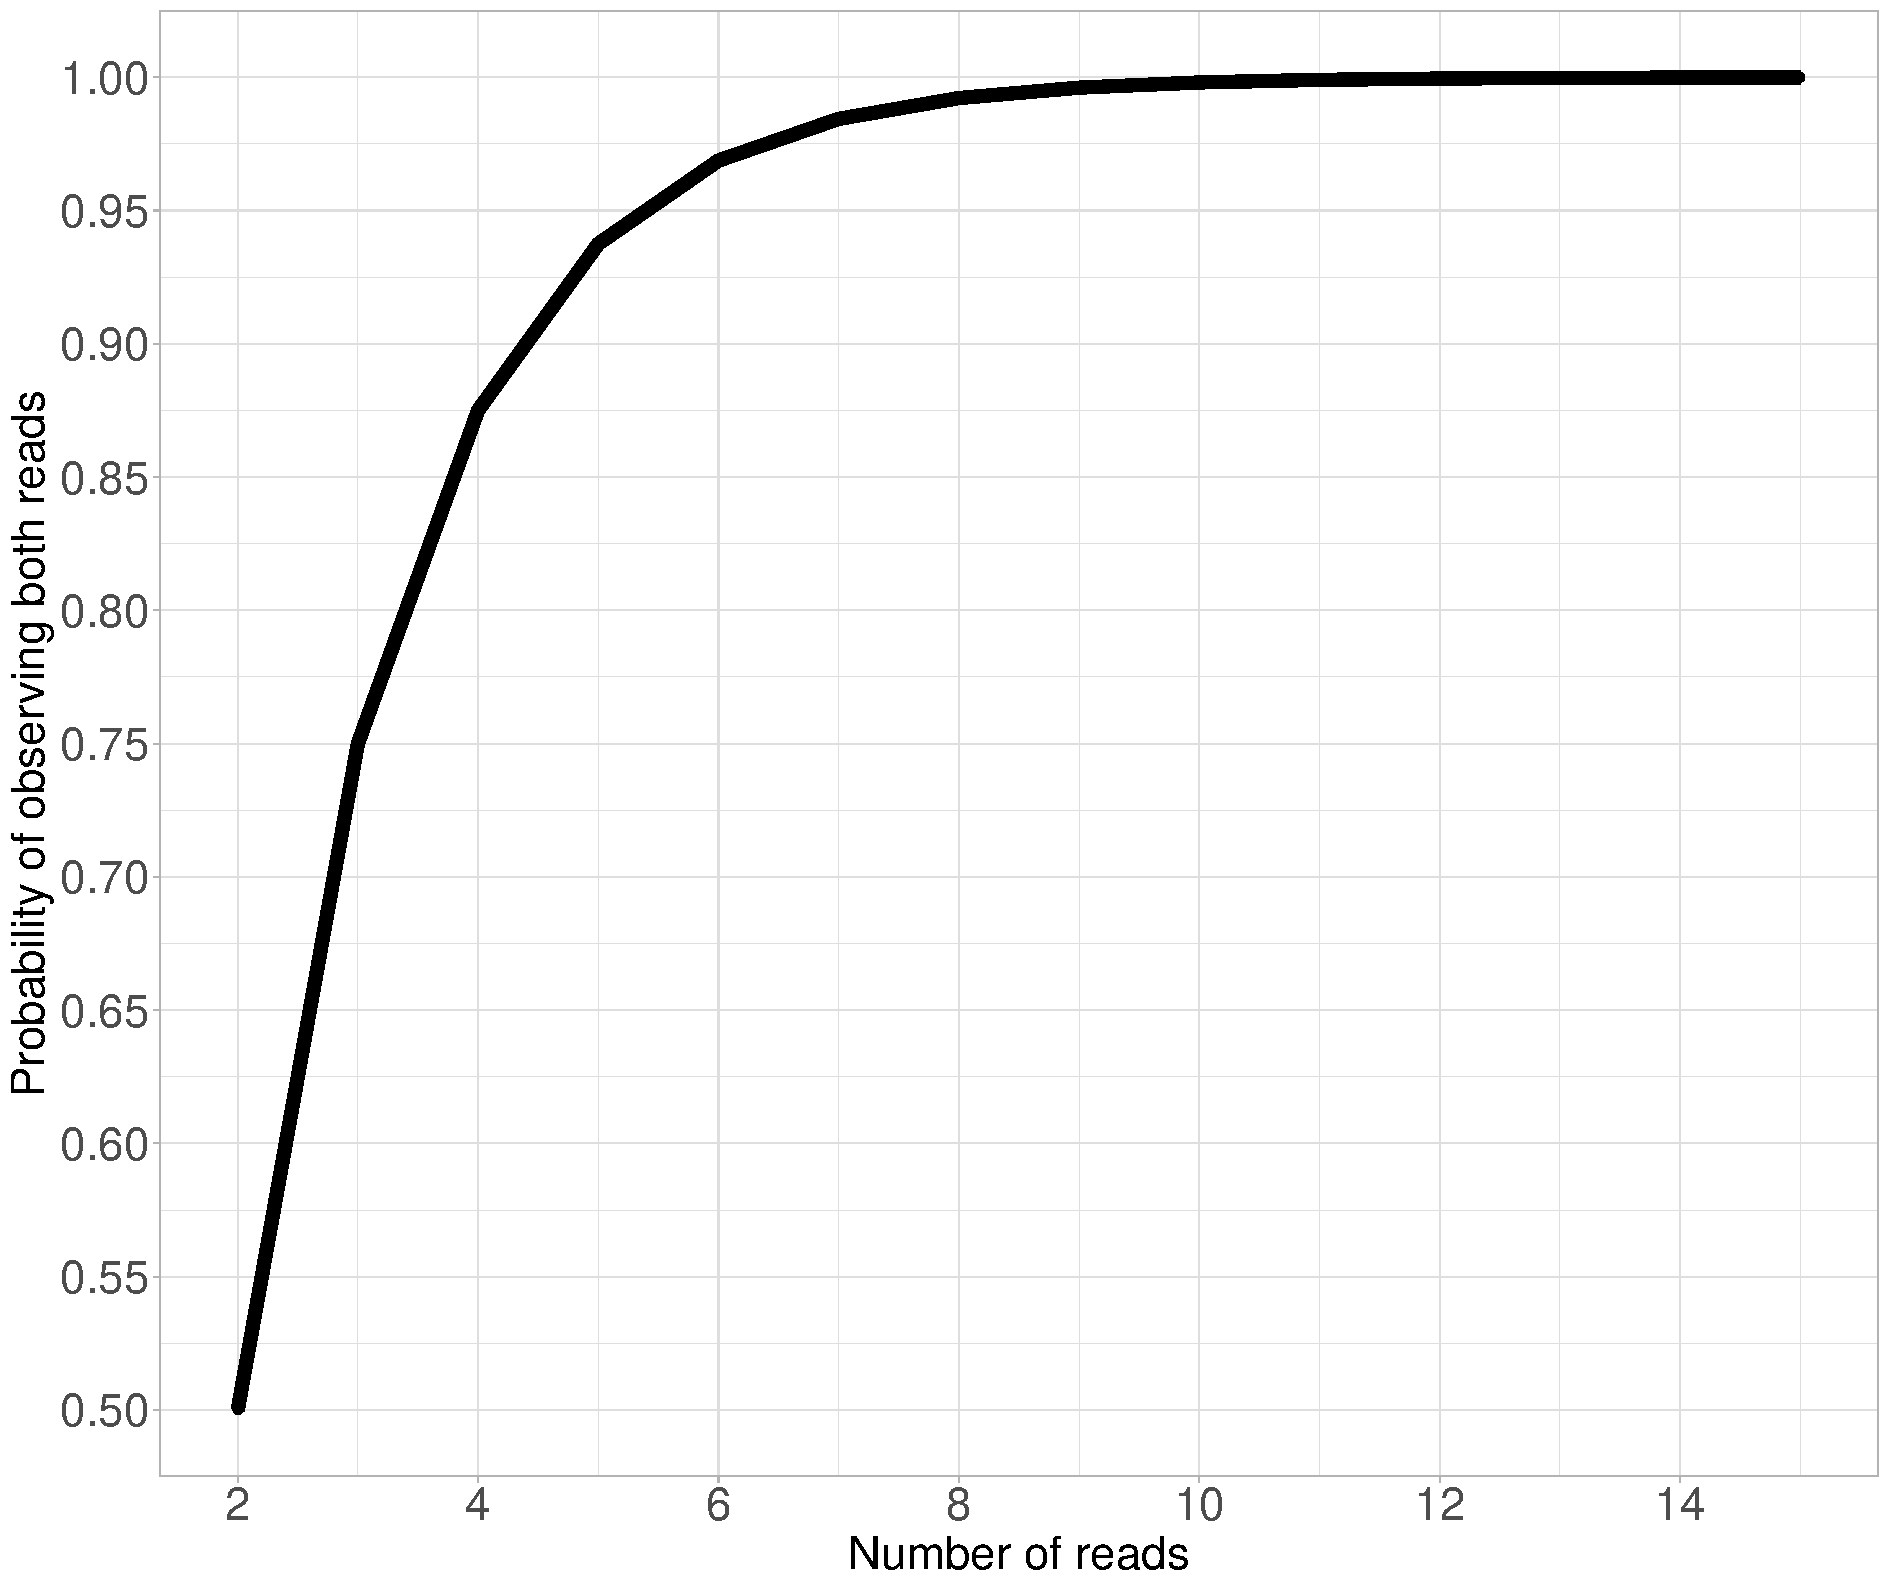
\includegraphics[width=1.0\textwidth]{../images/chapter1/het_prob.pdf}
    \caption{Probability of observing both reads at a heterozygous positions, given $x$ reads assuming equal probability of observing reference and non-reference alleles.}
    \label{fig:ProbabilityHetReads}
\end{figure}


\begin{table}
\centering
\begin{tabular}[t]{crr}
\toprule
\thead{Percentage \\ of SNPs retained} & Cornwall & Devon\\
\midrule
1 \% & 0.801 & 0.945\\
2 \% & 0.820 & 0.986\\
3 \% & 0.876 & 0.973\\
4 \% & 0.910 & 0.973\\
5 \% & 0.888 & 0.973\\
6 \% & 0.899 & 0.973\\
7 \% & 0.888 & 0.973\\
8 \% & 0.910 & 0.973\\
9 \% & 0.910 & 0.973\\
10 \% & 0.910 & 0.973\\
20 \% & 0.921 & 0.973\\
30 \% & 0.910 & 0.973\\
40 \% & 0.899 & 0.973\\
50 \% & 0.910 & 0.973\\
70 \% & 0.910 & 0.973\\
80 \% & 0.910 & 0.973\\
90 \% & 0.921 & 0.973\\
\bottomrule
\end{tabular}
\caption{Proportion of individuals correctly assigned to their population at different percentages of SNPs retained.}
\label{tab:prob_assignment_DevCorn}
\end{table}


In my painting of 5998 world-wide samples on the Human Origins array (described in Appendix section \ref{HumanOriginsAppendix}), the average number of segments that forms a recipient genome is 9764 (range: 1437-18,963). Given a genome-wide size of $\approx$ 3000Mb, this implies that an average `chunk' size (in Mb) is 3000/9764 = 307.2 $\approx$ 500kb, where a `chunk' is a set of contiguous SNPs matched to a single donor. Therefore, for each of the 12 different levels of SNP reduction used in my Devon/Cornwall analysis, I can calculate the average number of SNPs per 500kb chunks, and determine how many of these 500kb chunks are necessary to accurately distinguish individuals from Devon and Cornwall. To do so, for each reduced SNP percentage, I found the Cornwall/Devon classification score using only data from chromosome 22 (which has only W 500kb chunks), and using only chromosomes 21 and 22 (which has V 500Kb chunks), etc, continuing until the classification scores were equivalent to that when analysing all 22 autosomes at all 452,592 SNPs. In this way, for each reduced SNP percentage, I found the number of 500Kb chunks necessary to as accurately distinguish between Devon and Cornwall as in the case where we had analysed a full data set of 452,592 SNPs (Table \ref{table:windows_power_table_DevCorn}). I found results to be very similar to if chunk-size were instead defined as 250kb or 1Mb (Table \ref{table:windows_power_table_DevCorn}).


I repeated an identical analysis, including reducing the total number of SNPS, using individuals from the Mandenka and Yoruba ethnic groups rather than Devon and Cornwall.  

\begin{table}[!h]
\centering
\begin{tabular}[t]{lrrrc}
\toprule
\thead{Number of SNPs\\ retained} & 250Kb & 500Kb & 1Mb & \thead{Number of\\ SNPs per 500Kb \\Window}\\
\midrule
20,000 & 9356 & 4715 & 2388 & 3.3\\
25,000 & 6954 & 3509 & 1781 & 4.1\\
30,000 & 6272 & 3166 & 1607 & 5.0\\
35,000 & 4083 & 2064 & 1049 & 5.8\\
40,000 & 3099 & 1565 & 796 & 6.6\\
45,000 & 3602 & 1820 & 925 & 7.5\\
50,000 & 2612 & 1321 & 673 & 8.3\\
100,000 & 1304 & 661 & 338 & 16.6\\
150,000 & 1005 & 508 & 260 & 25.0\\
200,000 & 705 & 357 & 183 & 33.3\\
250,000 & 705 & 357 & 183 & 41.6\\
300,000 & 506 & 255 & 130 & 50.0\\
350,000 & 267 & 135 & 69 & 58.3\\
400,000 & 705 & 357 & 183 & 66.6\\
450,000 & 136 & 69 & 35 & 75.0\\
\bottomrule
\end{tabular}
\caption{Number of 250Kb, 500Kb or 1Mb windows required at different levels of SNP reduction to match the TVD assignment power of 500K fully genotyped SNPs for individuals in Devon and Cornwall. Note that the number of necessary 250kb and 500kb windows is roughly four and two times, respectively, the number of 1Mb windows, indicating the definition of window size makes little difference.}
\label{table:windows_power_table_DevCorn}
\end{table}

\begin{table}
\centering
\begin{tabular}[t]{lrrrr}
\toprule
\thead{Number of SNPs\\ retained} & 250Kb & 500Kb & 1Mb & \thead{Number of\\ SNPs per 500Kb \\Window}\\
\midrule
30,000 & 6272 & 3166 & 1607 & 5.0\\
35,000 & 3099 & 1565 & 796 & 5.8\\
40,000 & 3099 & 1565 & 796 & 6.6\\
45,000 & 2612 & 1321 & 673 & 7.5\\
50,000 & 3099 & 1565 & 796 & 8.3\\
100,000 & 1886 & 956 & 489 & 16.6\\
150,000 & 1304 & 661 & 338 & 25.0\\
200,000 & 506 & 255 & 130 & 33.3\\
250,000 & 267 & 135 & 69 & 41.6\\
300,000 & 506 & 255 & 130 & 50.0\\
350,000 & 506 & 255 & 130 & 58.3\\
400,000 & 506 & 255 & 130 & 66.6\\
450,000 & 267 & 135 & 69 & 75.0\\
\bottomrule
\end{tabular}
\caption{Number of 250Kb, 500Kb or 1Mb windows required at different levels of SNP reduction to match the TVD assignment power of 500K fully genotyped SNPs for individuals in from Mandenka and Yoruba ethnic groups.}
\label{table:windows_power_table_ManYor}
\end{table}

Guided by these results, for each ancient individual (n=587, median coverage=1.1x), I found the number of non-overlapping windows of sizes 250Kb, 500Kb or 1Mb that had $Y$ SNPs above $Z$ coverage, varying both Y and Z. 

Fig \ref{fig:avg_good_windows} shows the mean number of 500Kb windows per individual with at least $Y$ SNPs above $Z$ coverage, with individuals grouped into bins based on their mean coverage. Points are coloured yellow if, within the bin of coverage, samples have at least 2000 windows.

Samples less than 0.5x do not have enough windows, even if the threshold for a `good' SNPs is being covered by a single read. As is it not possible to call a heterozygous position with only a single read, this suggests that there are not enough non-imputed SNPs with enough coverage to match the power seen in full coverage individuals. For example, samples between 0.3-0.4x have approximately 1000 segments with $\geq$ 10 SNPs above 2x in coverage; Table \ref{table:windows_power_table_DevCorn} shows that 1565 windows of $\geq$ 8.3 SNPs is enough to match full power. However, as Figure \ref{fig:ProbabilityHetReads} shows, 50\% of these genotypes may not observe both reads if the position is heterozygous. Indeed, even when there are 3 reads covering a site, there is still a 25\% chance of not observing both alleles. Only the samples in the 2-5x coverage bin had enough windows when using a coverage threshold of 4 and 5 reads. 

This analysis therefore suggests that there are not enough regions with enough high quality SNPs at mean coverages less than 2x to reliably analyse using ChromoPainter.

\begin{figure}[htp]
    \centering
    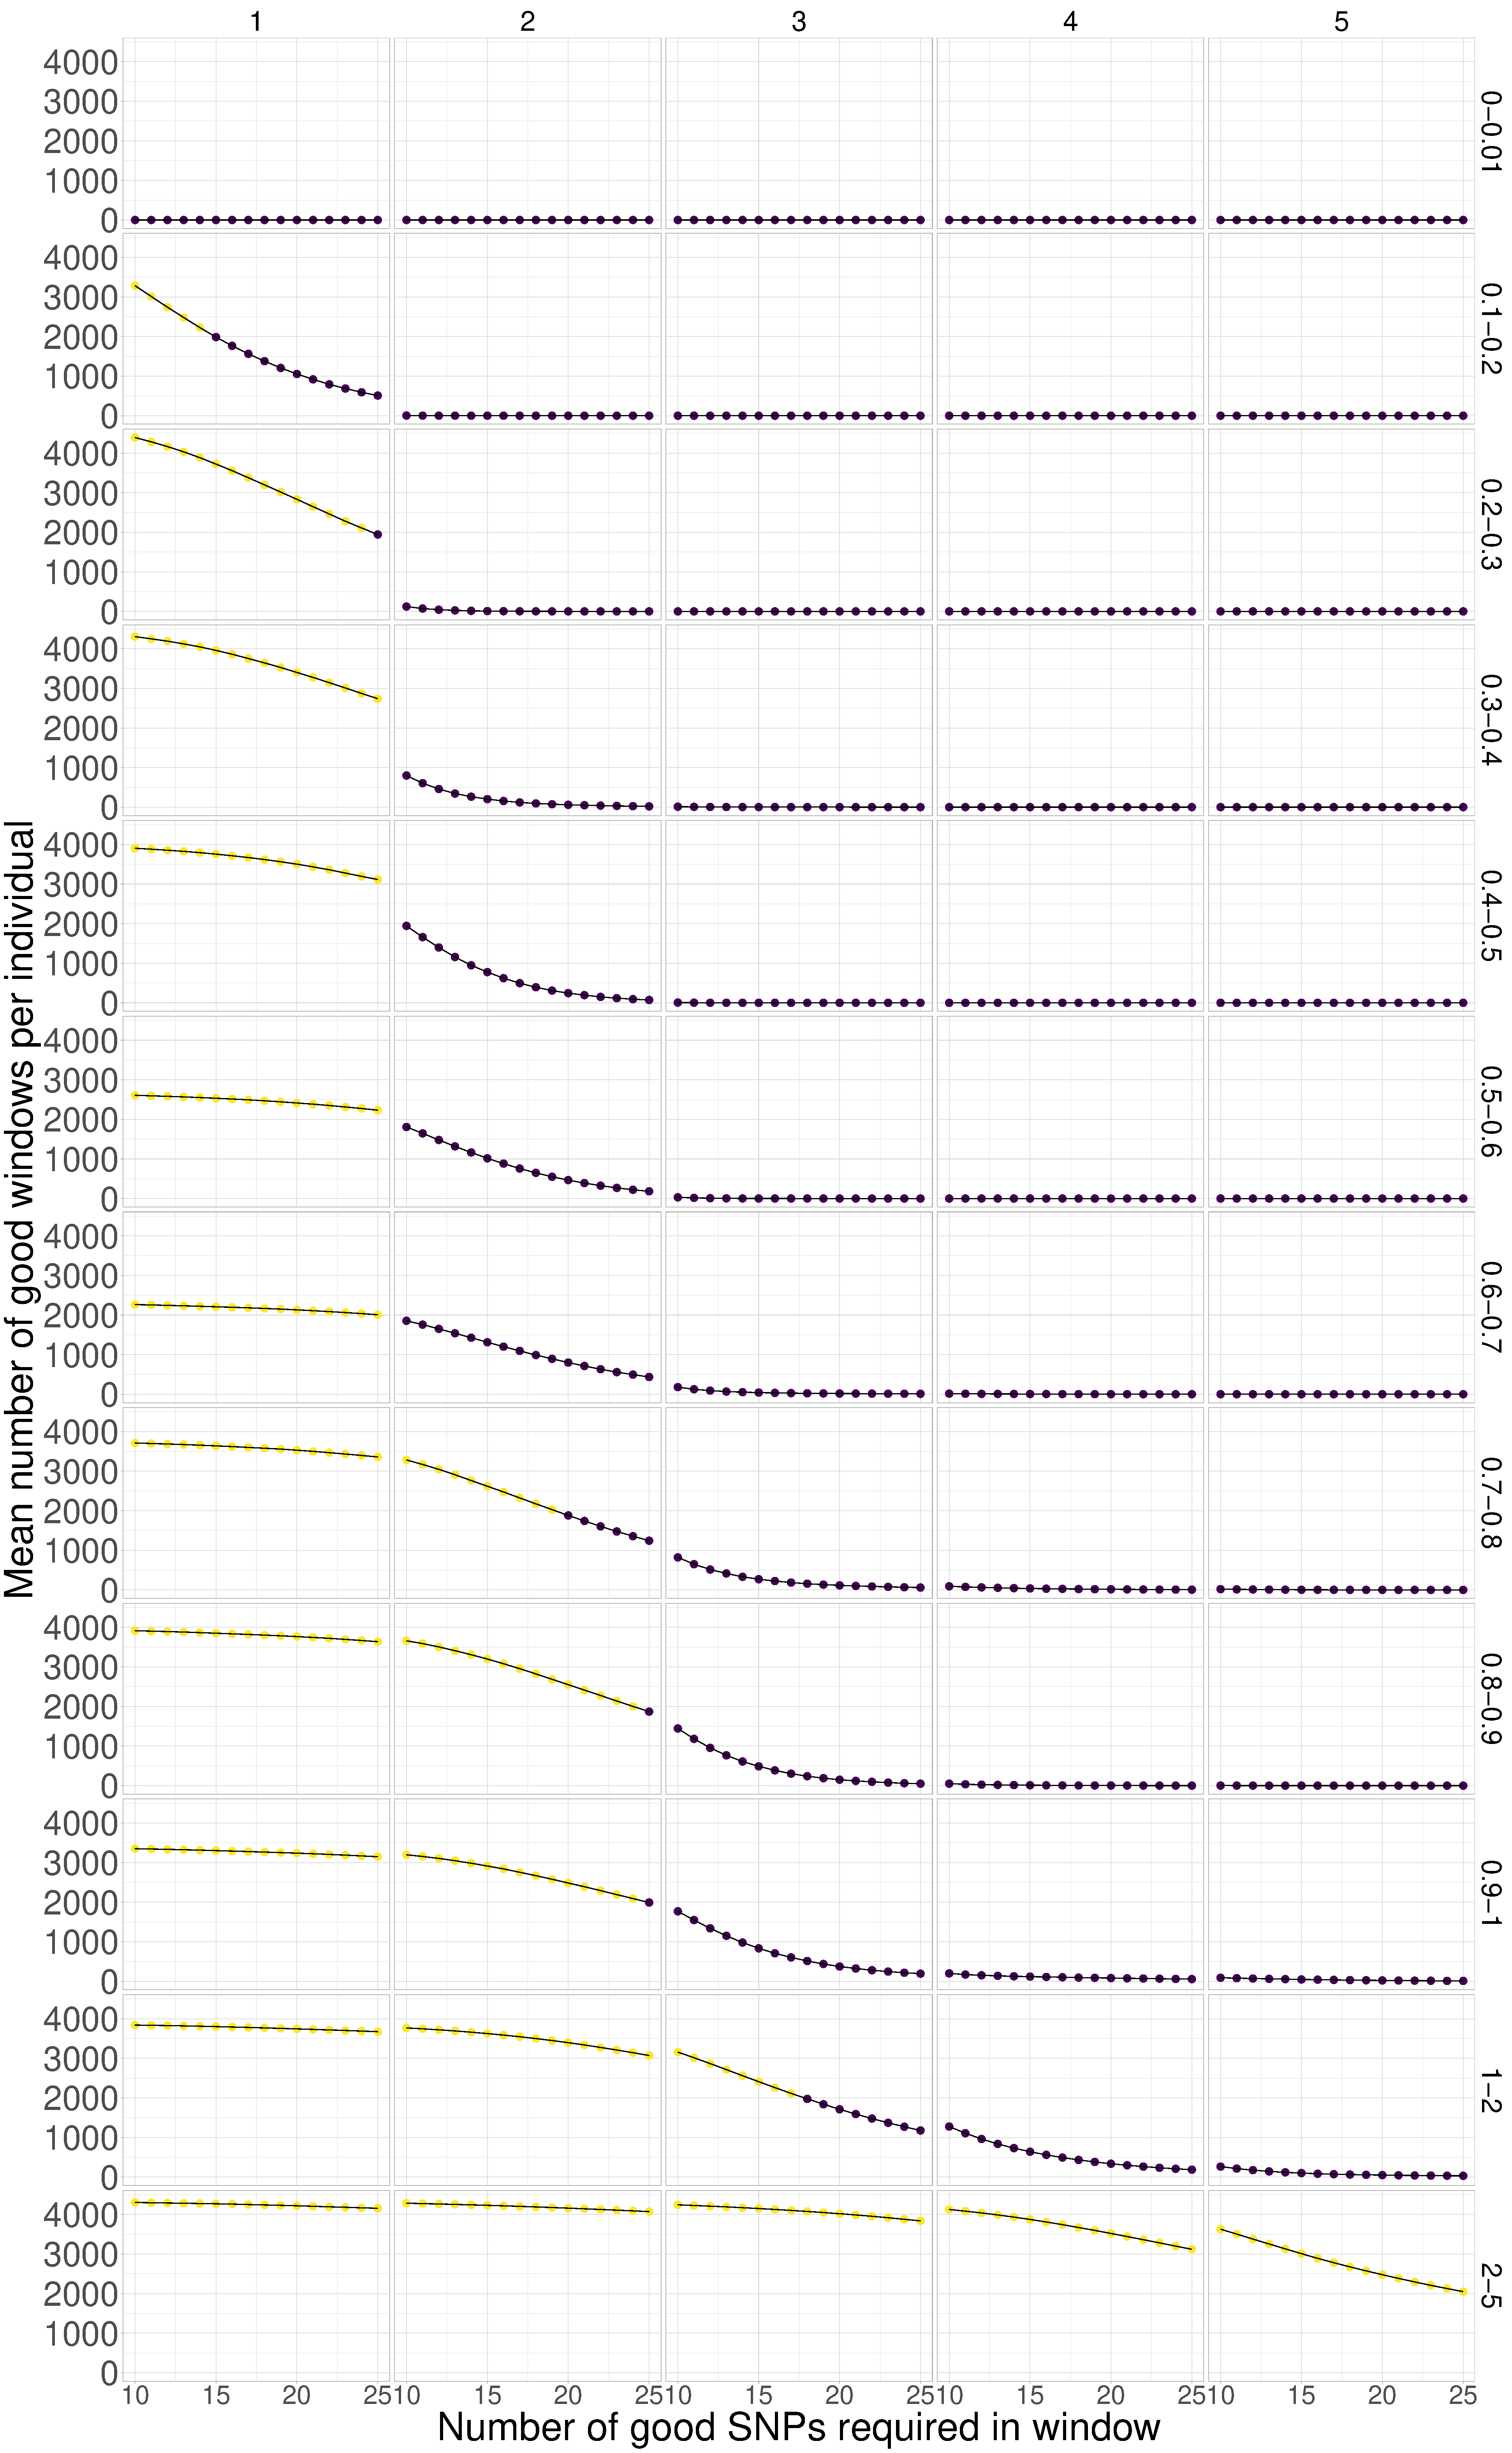
\includegraphics[width=1.0\textwidth]{../images/chapter1/avg_good_windows.pdf}
    \caption{Mean number of 500Kb windows (y-axis) within the genome of each ancient individuals within a given range of coverages (rows) with at least $Y$ SNPs (x-axis) above a particular coverage $Z$ (columns)}
    \label{fig:avg_good_windows}
\end{figure}


\begin{figure}[htp]
    \centering
    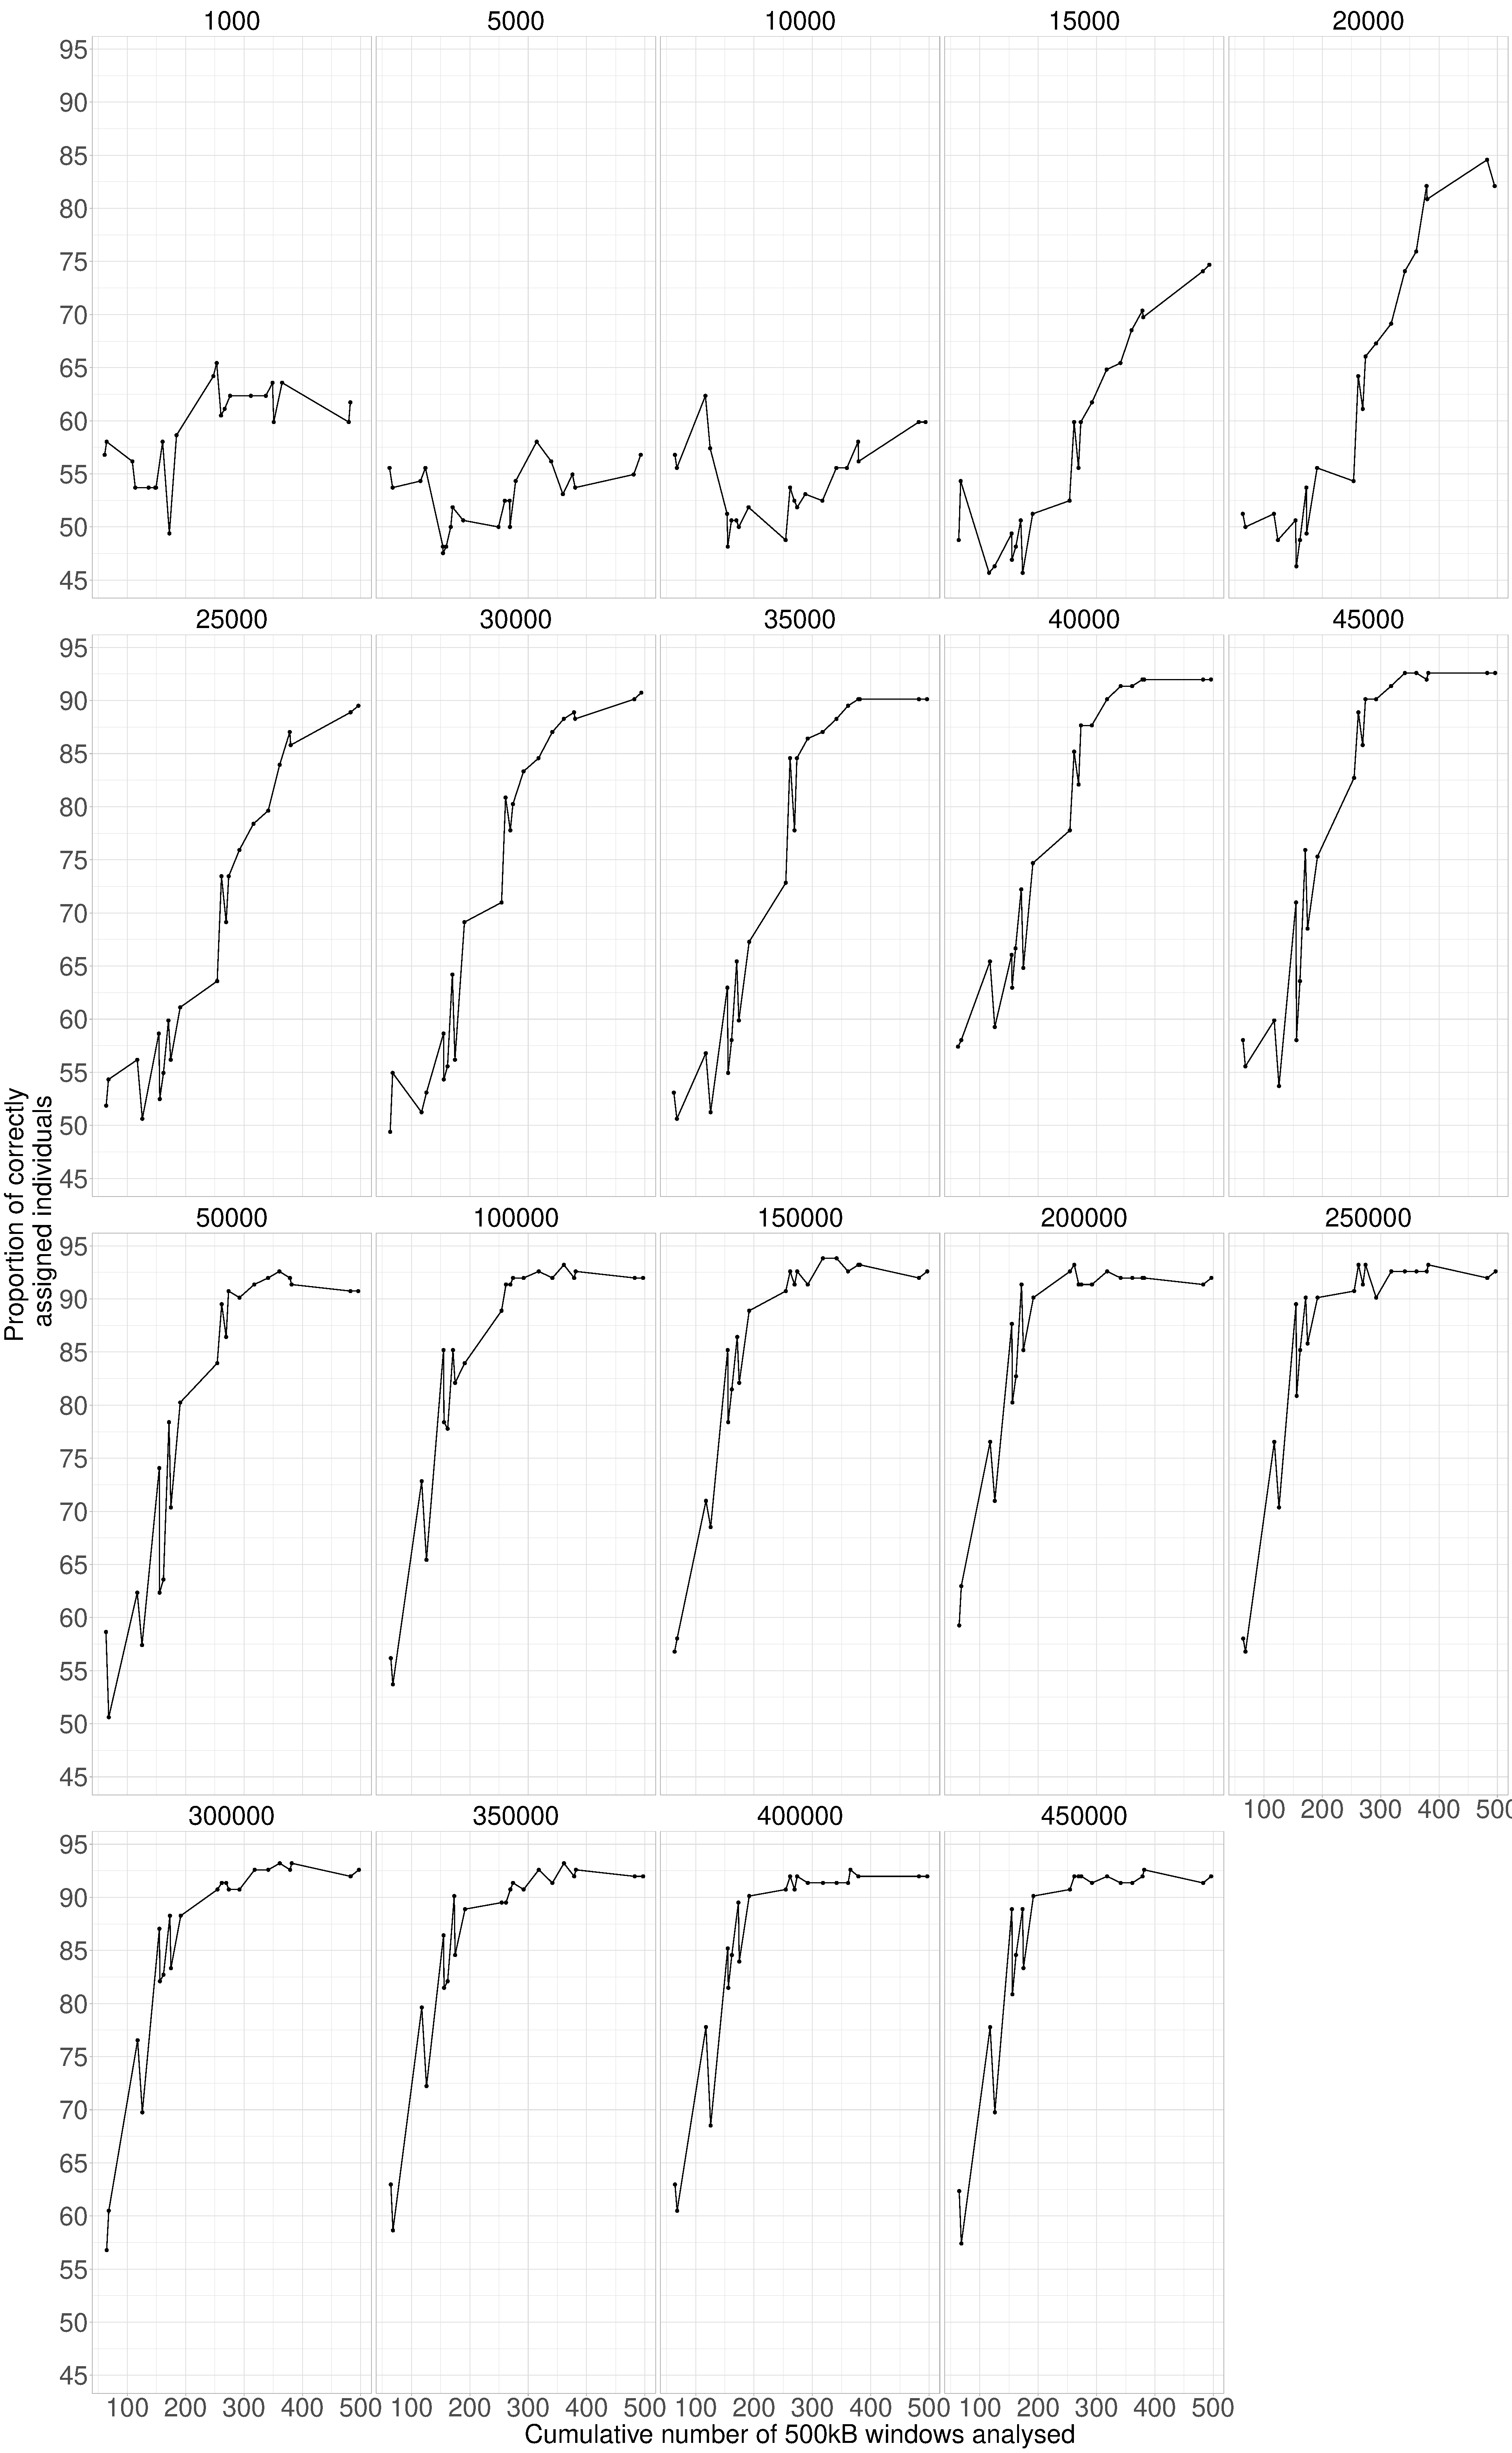
\includegraphics[width=1.0\textwidth]{../images/chapter1/cumulative_windows_val.pdf}
    \caption{The effect of adding 500kB windows on the ability to assign individuals from Devon and Cornwall to their respective populations. Each panel represents a different total number of SNPs used. X-axis gives the cumulative number of 500kB windows used in analysis. Y-axis gives the combined proportion of individuals assigned.}
    \label{fig:cumulative_windows_val}
\end{figure}


\section{Summary of Results and Discussion}

In this section I used a downsampling approach on five high-coverage ancient DNA samples to show that ChromoPainter analysis can be performed on samples down to 0.5x coverage without showing a significant deviation from the same sample at full coverage. In particular, ChromoPainter copyvectors, SOURCEFIND ancestry proportion estimates and Principle Component Analysis position all of 0.5x coverage and higher showed a good correspondence with the same metrics at full coverage. The 0.1x downsampled showed deviations from the full coverage samples which meant that they cannot currently be analysed reliably with ChromoPainter and its associated methods. I showed that imputation introduces bias into low-coverage samples that is manifested by those samples being shifted towards the centre of a PCA. 

I performed a range of analyses to try and recover useful haplotype information from low coverage samples and improve the performance of the analysis. Counter-intuitively, approaches such as removing SNPs with a low imputation quality and reference allele frequency did not improve the performance of ChromoPainter on low coverage samples. However, this is broadly consistent with a single previous study, which also showed that filtering the dataset for SNPs with a low imputation quality score did not substantially affect fineSTRUCTURE clustering \cite{Martiniano2017}. However, it also runs counter to studies which have shown filtering SNPs based on imputation quality score can significantly reduce the number of incorrectly imputed genotypes \cite{hui2020evaluating}. 

I also developed a modification to the ChromoPainter model which accounted for uncertainty in genotype calls; however it only marginally improved the performance of ChromoPainter on samples of 0.5x or higher. Again, this was surprising, as previously published methodology which accounts for genotype likelihoods when estimating IBD tracts has been shown to be effective \cite{Vieira2016}.

Finally, I used simulated data from present-day individuals to show that samples around 0.5x coverage can in theory be analysed with useful haplotype information, but that imputation is necessary for lower coverage samples.

Many of the analyses performed in this section only used a single target sample, as I did not identify a way to generate multiple downsampled individuals from the same population. For example, the SOURCEFIND analysis I performed  used a single target downsample when estimating ancestry proportions. This differs from a typical ancient DNA analysis, such as those of Margaryan et al \cite{margaryan2020population}, where there may be up to 20 low coverage samples per population. This number may increase in the future as the technology to generate ancient DNA improves. Leveraging information across multiple samples from the same population  would improve the accuracy of population-wide ancestry or admixture estimates, for example. Thus, the results presented in this section which used a single target individual may underestimate the ability to analyse low-coverage samples. It may be possible to accurately analyse 0.1x samples if there are multiple samples per population. 

In this section I used present-day individuals to estimate the number and size of chunks needed to retain haplotype information. This was because present-day individuals are simpler to analyse; the populations are better defined than in ancient samples (i.e. it is possible to only include individuals whose grandparents were born within 100kM of a target location), are of uniform coverage and contain many more individuals per population. Thus, using present-day individuals removes potentially confounding factors that may be present when analysing ancient samples. However, using present-day samples to draw conclusions about ancient samples may lead to underestimating the number of SNPs per window required. As the present-day samples had been genotyped high-quality DNA samples and a genotpying array, each genotype can be called with a high confidence. This is not the case with ancient samples, where each SNP may be covered by a small number (<3) of reads.

For the imputation and phasing reference panel, I used the 1000 genomes dataset which contains around 6000 haplotypes. The Haplotype Reference Consortium contains roughly 10 times as many haplotypes and thus offers substantial gains in the potential accuracy of genotype imputation \cite{rubinacci2021efficient}. I did not use the HRC owing to difficulties in obtaining access to the data; however, I expect that future studies which use this resource will be able to analyse ancient DNA samples of low coverage to a higher degree of accuracy. 

Whilst I did not interrogate the range of coverages between 0.1-0.5x, this could be an avenue for future research.




\chapter{Investigating the sub-continental ancestry of ethnic minorities within the U.K. Biobank from sparse genotype data}
\label{chapterlabel3}

\section{Introduction}

From a genetic standpoint, the British population is one of the most studied in the world, with many studies sequencing or genotyping individuals from across the U.K (e.g. \cite{bycroft2018UK, Leslie2015, turnbull2018introducing, UK10k2015UK10k}). These projects have been primarily aimed at researching the genetic basis of disease, but have also been used to investigate population history, substructure  and the relationship of different sub-populations in the U.K. to other European countries \cite{Leslie2015, schiffels2016iron, liu2020human}.  

The U.K. is also an ethnically diverse country, with 13.8\% of individuals belonging to ethnic minority groups (source: \href{https://www.ons.gov.U.K./peoplepopulationandcommunity/populationandmigration/populationestimates/articles/researchreportonpopulationestimatesbyethnicgroupandreligion/2019-12-04}{ONS survey}). Groups of people from across the world have migrated to the U.K. at different periods in the previous three centuries, driven by the legacy of colonialism \cite{nasta2005voyaging}, the transatlantic Slave Trade and a variety of other reasons. Despite this, the roughly 9 million ethnic minorities within the U.K. remain relatively understudied in the context of genetics. For example, every one of the 27 papers in the GWAS catalogue with "U.K. Biobank" in the title, and two others presently in the catalog curation queue, limited their analyses to subgroups described in various terms as "White British", "British", "European", "White European", "Caucasian" or "White" \cite{manolio2019using}. The primary reason for this is reasonable concerns over the confounding effect of population substructure within a cohort \cite{hellwege2017population}; retaining a more genetically homogeneous cohort is one strategy to mitigate this. 

However, removing ethnic minorities from GWAS analyses is problematic, as evidence is mounting that the results from GWAS, including Polygenic Risk Scores (PRS), may not be transferable to other populations if they have been conducted in cohorts of exclusively European individuals \cite{kuchenbaecker2019transferability, martin2017human, bustamante2011genomics}. The reasons for this are not yet fully understood, but it is thought that differences in LD structure may be at least partially responsible \cite{vilhjalmsson2015modeling}. Ethnic minorities may therefore miss out on the advances in healthcare driven by large-scale genomic projects. 

Understanding, and correcting for, population structure is an important step towards including a diversity of ancestries in GWAS. Several recent studies have shown the power of methods which explicitly model linkage between neighbouring markers when controlling for population structure, relative to traditional approaches such as PCA. Zaidi and Mathieson (2020) \cite{zaidi2020demographic} showed that whilst it is not possible to correct for recent population stratification using principal components of common variants, correcting using a matrix of pairwise IBD sharing is effective. Similarly, it has been shown (S.Hu, personal communication of unpublished data) that incorporating principle components did not eliminate significant associations between genetic variants and birth location in UK Biobank participants. However the significant hits disappeared when corrected for using a ChromoPainter coancestry matrix, generated by painting target samples against a set of reference individuals and using the resulting painting profile as covariates in the association test. Byrne et al also eliminated significant associations with birth place in a cohort of Dutch individuals, by painting samples using PBWT-paint, a method closely related to ChromoPainter \cite{byrne2020dutch}. 

Other recent studies have leveraged advances in algorithm development, such as the positional Burrows-Wheeler transform, to perform haplotype-based analyses on Biobank-scale datasets. Saada et al (2020) detected around 214 billion IBD segments across 487,409 individuals in the U.K. Biobank, obtaining enough information to estimate birth location to within 45 km, demonstrating the power of haplotype-based approaches on large datasets. However, their method only estimated pairwise IBD between individuals rather than comparing each individual to \textit{all} other individuals in the dataset. The latter approach is more powerful at detecting recent shared ancestry because it finds who an individual shares ancestry with overall \cite{LawsonFalushReview}. Additionally, Saada et al only considered self-identified White British individuals. Zhou et al (2020) recovered a similar number of IBD segments within the U.K. Biobank (231.5bn), also using a PBWT-based method \cite{ZHOU2020426}.


Recent studies have outlined the power of haplotype-based approaches in inferring the population histories of different African ethnic groups \cite{lopez2021evidence, StructureEthiopians2021, gurdasani2019uganda}. Therefore, it seems natural to extend the approaches of Saada et al and Byrne et al to exploring the ancestry and structure of individuals of recent African ancestry in the U.K. Biobank as a first step to including a wider diversity of ethnicities in association studies. 

Additionally, but no less importantly, there is intrinsic value in exploring the ancestry of individuals (ethnic minorities in the U.K.) who have typically been excluded from analyses. Excluding individuals based upon their ethnicity presents other issues; individuals who registered for the U.K. Biobank undertook a series of extensive tests and not including their data in studies seems to be ethically dubious at best \cite{peterson2019genome}.


Therefore, to investigate the African ancestry of U.K. Biobank individuals, I will leverage a recently compiled dataset, hereafter referred to as `Human Origins'. At the time of writing, it is the most detailed dataset of genotype data from African individuals in terms of the number of ethnolinguist groups represented. Whilst the dataset contains individuals from across Africa, it contains particularly large numbers of individuals from South Africa (n=104), Cameroon (n=567) and Ghana (n=211), which are countries known to have contributed immigrants to the U.K. Of the 5998 samples in the Human Origins dataset, 1,518 are previously unpublished, including all samples and 188 populations from Sudan, Nigeria, Ghana and The Democratic Republic of Congo. Therefore, this dataset is ideal for use as a reference panel to investigate the ancestry of ethnic minorities within the U.K. Biobank. In particular, given our newly acquired data comes from parts of west Africa that may well represent sources of African ancestry among UK minority groups, I chose to investigate individuals with recent African ancestry. However, these results should in theory be equally applicable to other non-European populations, such as those from east and south Asia. 

One potential issue is that only 70,776 SNPs overlap between the U.K. Biobank and Human Origins genotyping arrays. This is much lower than the number used in a typical ChromoPainter analysis, which is usually between 500,000 and 700,000. Using a low number of SNPs in the analysis may reduce the power to infer accurate ancestry proportions, in particular for haplotype-based methods since haplotype information depends on SNP density. Therefore, one option is to impute the non-overlapping SNPs using a reference panel. However, the effect of imputation on ChromoPainter-style analyses has yet to be fully investigated. It is possible that imputing a large number of positions may introduce biases, particularly towards populations which are present in the reference panel. Studies have shown repeatedly that genotypes in non-European individuals are imputed less accurately compared to European individuals when using a primarily European reference panel \cite{delaneau2018integrative, taliun2021sequencing}. Accordingly, we can ask whether it is preferable to retain a smaller number of non-imputed SNPs or a larger number SNPs, some of which have been imputed. My work in Chapter 2 showed that imputation introduced bias towards European populations prevalent in the reference panel; in this chapter, I will extend that analysis to determine the effect of imputation on population assignment in African ethnic groups. 

This chapter will focus on two questions. Firstly, I will evaluate the effect of using imputed genotypes on the validity of ChromoPainter analysis in African individuals, similar to analyses I performed in Chapter 2 but tailored to my U.K. Biobank analysis. Secondly, I will compare genetic variation patterns of U.K. Biobank participants with recent African ancestry to the Human Origins dataset populations, in order to shed light on their ancestral origins.

\section{Methods}

\subsection{U.K. Biobank data access and initial processing}

The U.K. Biobank dataset contains genotype data for 488,378 individuals at the time of writing (\url{https://www.U.K.biobank.ac.U.K./}). Access was obtained to study the U.K. Biobank dataset via UCL Genetics Institute (ref number 51119, principal investigator = D.Curtis). 

I obtained the U.K. Biobank genotype data, consisting of 488,377 individuals genotyped at 784,256 genome-wide SNPs on the U.K. Biobank Axiom Array. I will hereafter refer to this dataset as the `non-imputed' data, as all SNPs were directly genotyped without imputation. I used plink2 \cite{purcell2007plink} to convert the binary plink files to \texttt{.bcf} format. 

I also obtained U.K. Biobank data, which had already been imputed to approximately 96m SNPs from the original 784,256, using the combined references of the Haplotype Reference Consortium (HRC) and UK10K haplotype resource. I will hereafter refer to this data as the `imputed' data. Full details of imputation can be found in the paper of McCarthy et al (2016) \cite{mccarthy2016reference}. The imputed data was downloaded and converted from \texttt{.bgen} to \texttt{.bcf} format using qctool2 (\url{https://www.well.ox.ac.U.K./~gav/qctool_v2/}). 

I therefore had two separate datasets; `imputed' and `non-imputed', containing the same individuals and differing only in whether or not imputation had been used to increase the total number of SNPs.

\subsection{ADMIXTURE analysis}

I am primarily interested in using ChromoPainter \cite{Lawson2012} to explore the ancestry of ethnic minorities in the U.K. Biobank. However performing ChromoPainter analysis on the entire U.K. Biobank dataset (n=488,377 individuals) is computationally infeasible. Thus, I chose to analyse only those individuals with more than 50\% non-European ancestry. The ADMIXTURE algorithm is a fast and accurate way to estimate continental-scale ancestry proportions \cite{alexander2009fast} and is therefore ideal for the task identifying individuals with  more than 50\% non-European ancestry in a large cohort. 

I LD-pruned the non-imputed U.K. Biobank dataset using using \texttt{plink --indep-pairwise 50 10 0.02} \cite{purcell2007plink}, leaving a total of 70,776 bi-allelic SNPs. I then subsetted the 1000 Genomes dataset down to the 70,776 SNPs retained in the U.K. Biobank dataset and merged the two datasets using \texttt{bcftools --merge}. Thus, I had a dataset containing all U.K. Biobank and 1000 Genomes individuals, genotyped at 70,776 SNPs.

I ran ADMIXTURE in supervised mode using the argument \texttt{--supervised} and fixed the four reference populations as GBR British, Nigeria Yoruba, Han Chinese and Gujarati Indian from the 1000 Genomes dataset. These populations were chosen as they represent a broad division of worldwide populations into African, European, East Asian and South Asian; for the purposes of this particular analysis, it was not necessary to include finer-scale populations. The rest of the arguments were left to default.

Individuals with at least 50\% ancestry from Nigeria Yoruba were carried into later analysis; I refer to these as `selected' Biobank individuals.

\subsection{Data preparation - Human Origins}

To determine the ancestry of U.K. Biobank individuals, I compared their SNP patterns to populations/ethnic groups from different parts of the world to infer which populations they share recent ancestry with. As I am particularly interested in studying individuals with recent African ancestry, I used the so-called `Human Origins' reference dataset for this purpose, as it contains individuals from 349 different ethnic groups from across Africa and 535 world-wide groups in total (Fig. \ref{fig:HumanOriginsMap}). Full details of processing can be found in Appendix section \ref{HumanOriginsAppendix} .

\begin{sidewaysfigure}
	    \centering
	    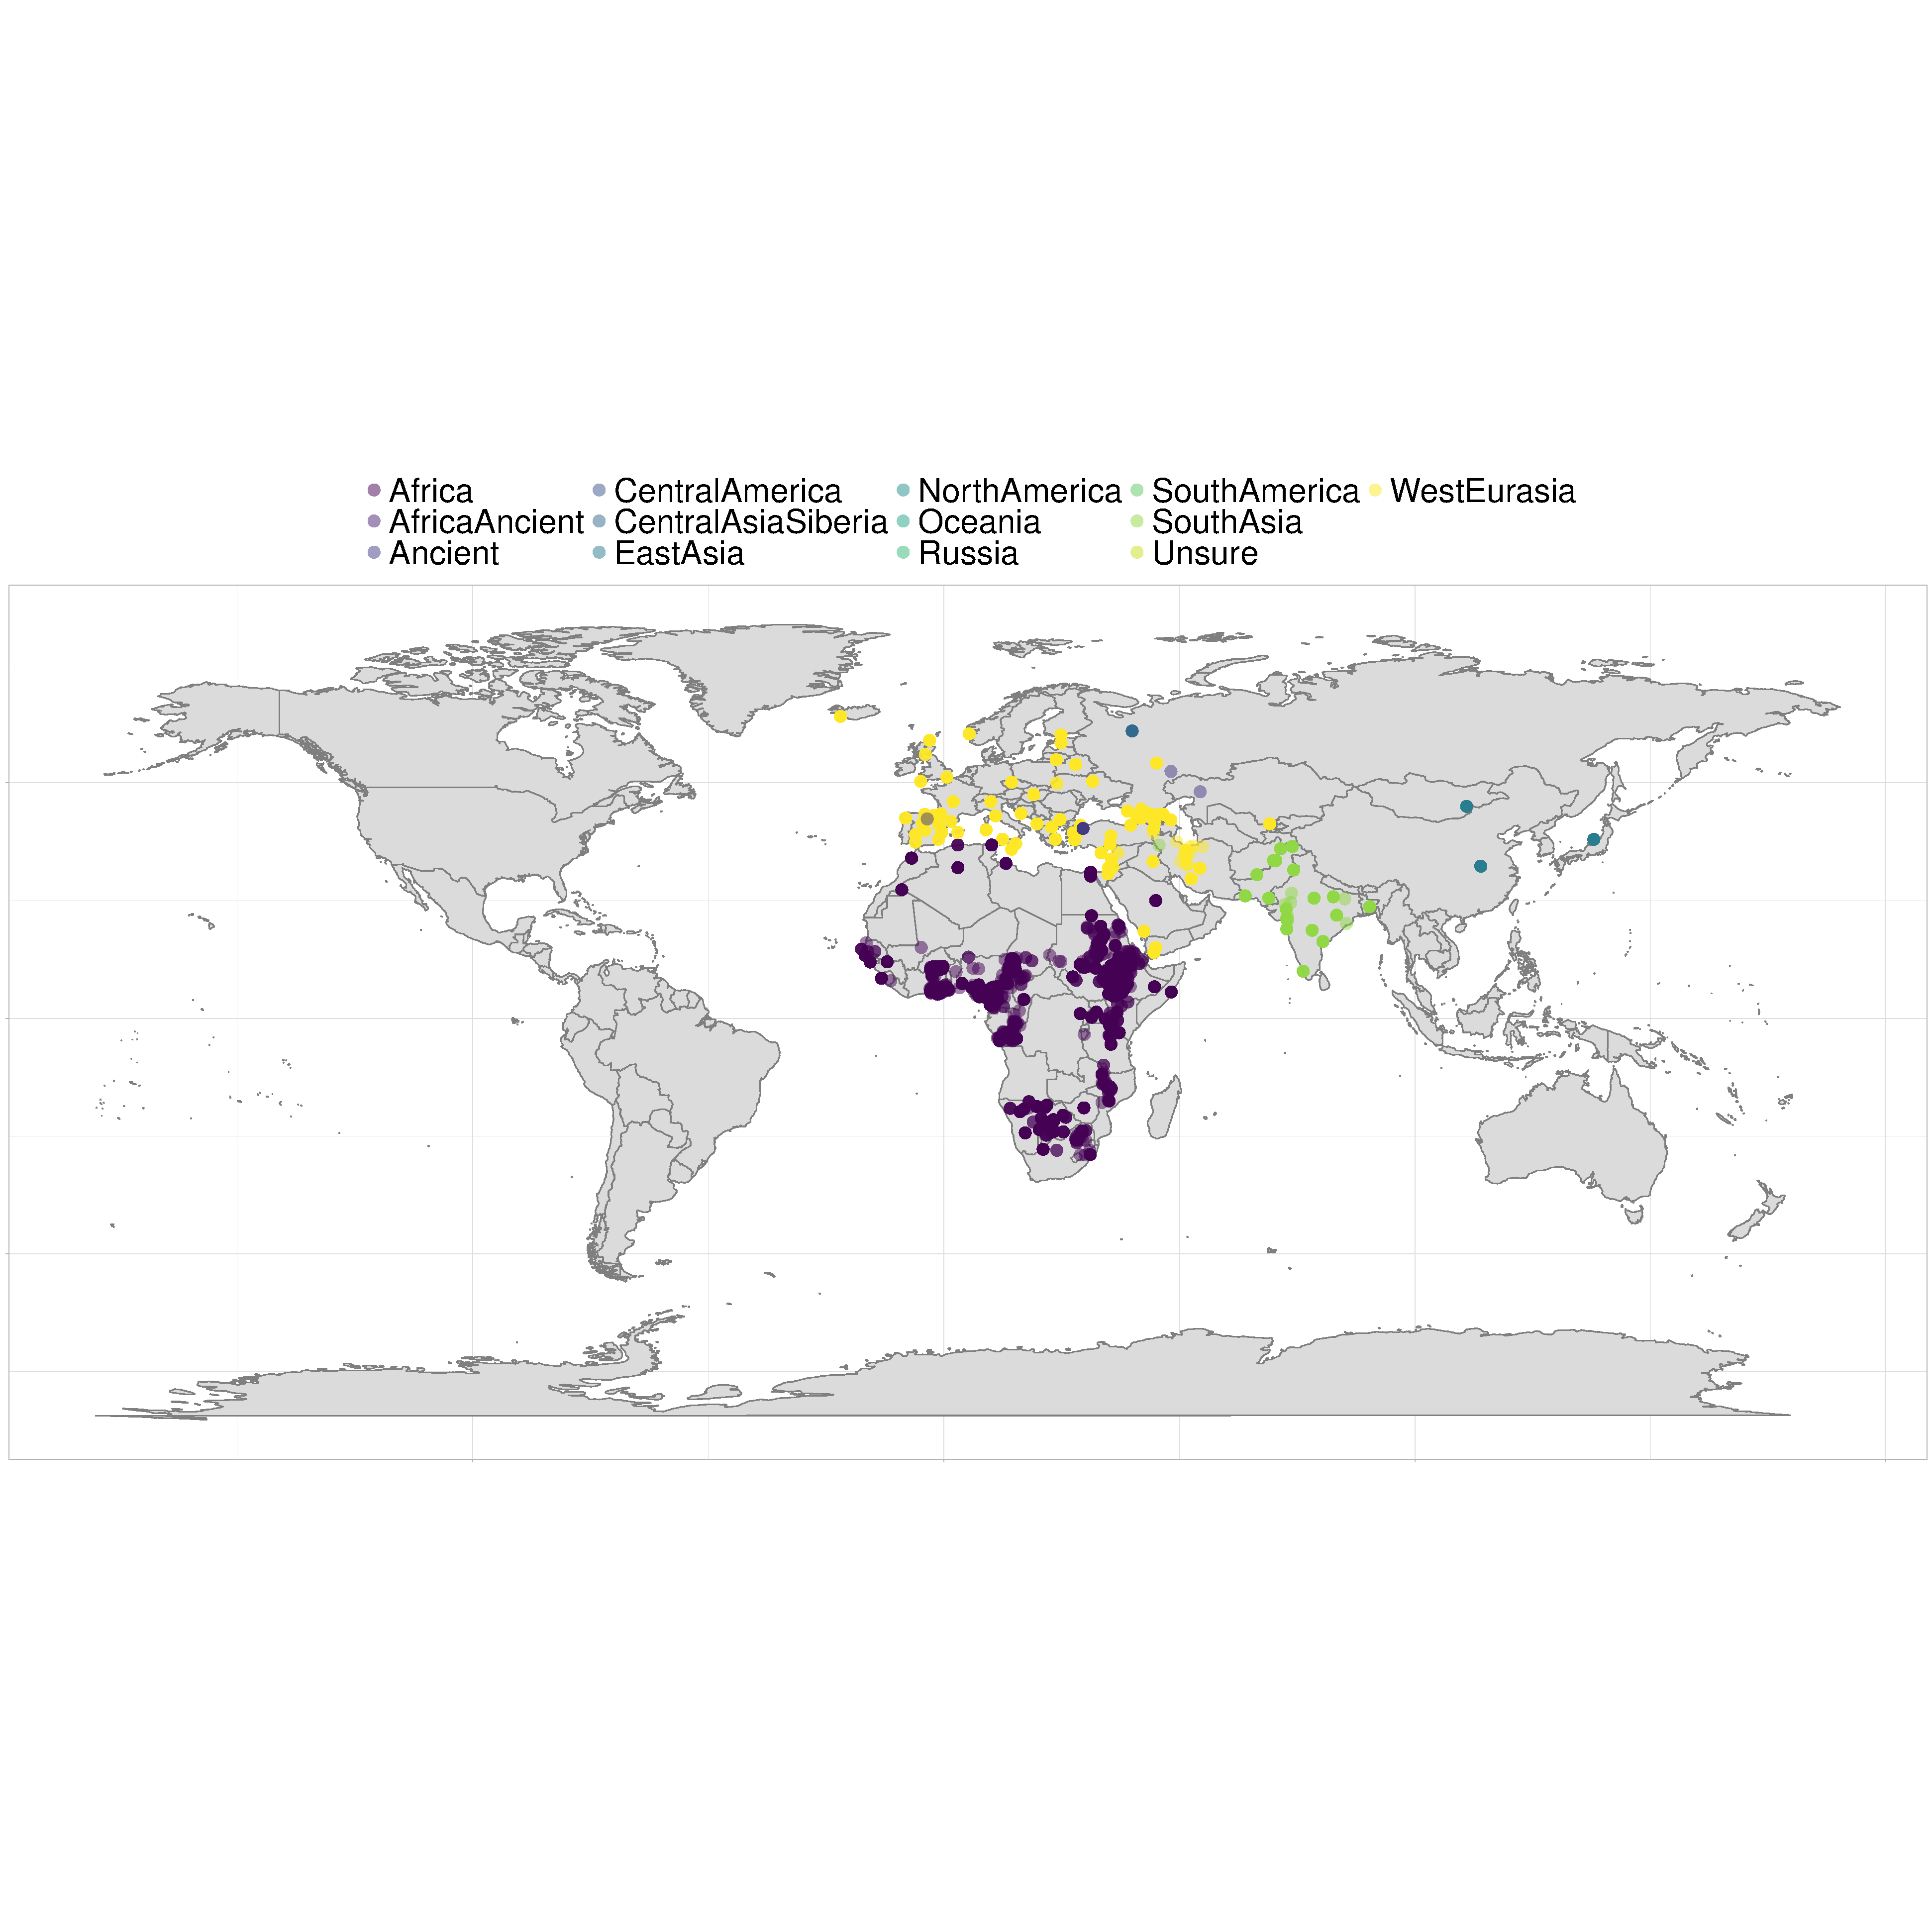
\includegraphics[width=1.0\textwidth]{../images/chapter3/HumanOriginsMap.pdf}
	    \caption{Map of Human Origins populations.}
	    \label{fig:HumanOriginsMap}
\end{sidewaysfigure}

\subsection{Data merge - non-imputed data and Human Origins}

I used \texttt{bcftools --merge} to merge 5,998 reference Human Origins dataset individuals with 8,476 UK Biobank participants that had $\geq$50\% African ancestry, using the gt-conform utility from Beagle (\url{https://faculty.washington.edu/browning/conform-gt.html}) to remove any inconsistent positions. This dataset contained 65,749 non-imputed SNPs that overlap between the Human Origins and UK Biobank arrays. I phased this dataset with shapeit4 \cite{delaneau2018integrative} using \texttt{--pbwt-depth 8}, the b37 genetic map and all other parameters set as default.  

\subsection{Data preparation - imputed data}

I similarly merged the imputed UK Biobank data with the Human Origins reference dataset at 525,566 SNPs that were genotyped in Human Origins, and phased this dataset with shapeit4, using the same settings as for the non-imputed data.

\subsection{ChromoPainter}

For both of the imputed and non-imputed datasets, I used ChromoPainter to infer the proportion of genome-wide DNA that each UK Biobank and Human Origins reference individual matches to individuals from each Human Origins reference population. 

An alternative option to using ChromoPainter would be to use PBWT (positional Burrows-Wheeler transform) paint (\url{https://github.com/richarddurbin/pbwt/blob/master/pbwtPaint.c}), a fast approximation to ChromoPainter which provides approximately the same output and is scalable to large sample sizes \cite{byrne2020dutch}. However, it is not possible to provide a reference panel and each haplotype must be compared to all others in turn. This would be much less efficient and would not allow me to take full advantage of the Human Origins dataset. 

\subsection{SOURCEFIND}

I estimated ancestry proportions for each of the selected U.K. Biobank individuals using SOURCEFINDv2 \cite{Chacon-Duque2018}. I used the combined painting from the section above. I analysed each U.K. Biobank individual with more than 50\% African ancestry separately, using all Human Origins populations as surrogates. I left all parameters as default. 

\subsection{Imputation bias test} \label{sec:ImputationBiasTest}

The imputed U.K. Biobank dataset was imputed using a reference panel containing the Haplotype Reference Consortium. Whilst this reference panel contains many European populations, it contains relatively few from Africa. Imputing variants in non-European individuals using a reference panel that is primarily composed of European individuals may lead to biased or inaccurate imputation \cite{huang2011haplotype}. Given I am particularly interested in analysing individuals with recent African ancestry in the U.K. Biobank, it is important to determine whether this is the case.  

An obvious way to test this would be to compare a painting on the \textbf{U.K. Biobank} individuals using datasets comprised of a majority imputed and non-imputed SNPs. However, this is not possible; the samples in the U.K. Biobank dataset do not have any associated population or ethnic group labels beyond broad self-identified categories. Accordingly, it would not be possible to mask their ethnic group and attempt to guess it using only the genetic data, an approach which I use for the Human Origins data in this chapter.

Therefore, I used the Human Origins dataset, where I could control whether or not SNPs are imputed and mask population labels. I submitted the full Human Origins reference dataset (5998 individuals and 560,420 SNPs) to the Sanger Imputation Server (\url{https://imputation.sanger.ac.U.K./}), which uses the full Haplotype Reference Consortium (HRC) as a reference panel for imputation. 
I subsetted the imputed Human Origins dataset down to SNPs present in the U.K. Biobank array, leaving 727,325 positions present in the imputed Human Origins dataset and then randomly removed SNPs until 500,000 remained. Although the number of SNPs still differ, my previous research in Chapter 2 shows that increasing the number of SNPs beyond 400,000 does not affect the ability to correctly assign individuals to populations (Appendix section \ref{sec:SNP_Count_Assignment_DevCorn}). I phased the imputed and non-imputed datasets separately using shapeit4 at default settings. 

To  therefore determine whether using the imputed or the 70,000 SNP Human Origins dataset is better in this scenario, I performed a painting using (i) the full 560,442 genotyped SNPs, (ii) 64,762 genotyped SNPs overlapping UK Biobank, and (iii) 500,000 SNPs that include the 70,000 genotyped SNPs and 430,000 SNPs imputed using the HRC reference. I performed painting (ii) in both linked and unlinked mode to determine whether there is haplotype information using 70,000 SNPs.

For each of the three datasets described above, I selected all ethnic groups from Nigeria, Cameroon and Ghana which had five or more individuals (n=51 populations, n=1203 individuals) and split each population randomly in half, into `donors' and `recipients'. I painted all recipient populations (n=51) using all donor populations (n=51) using a leave-one-out approach (motivation for this approach given in Appendix section \label{sec:leave_one_out}). I tested the information content of each painting by counting how often individuals copy more from individuals in their own populations than individuals from other populations. I also counted the number of times a population had the lowest TVD (motivation and description of TVD given in appendix section \ref{sec:appendixTVD}) with its own population (Table \ref{table:TVD_copying}).

\section{Results}

\subsection{4\% of U.K. Biobank individuals have at least 50\% non-European ancestry}

Performing ChromoPainter analysis on the 488,378 individuals in the U.K. Biobank would be computationally unfeasible; therefore I first performed supervised ADMIXTURE on all U.K. Biobank individuals. In order to identify individuals with at least 50\% African ancestry, I set $K=4$ supervision clusters that were defined using European (CEU), Gujarati, Han Chinese and Yoruban reference individuals from the 1000 genomes dataset. I then carried forward individuals with more than 50\% ancestry from Yoruba to later ChromoPainter analyses.

In total, there were 8476, 2653, 9171 individuals with at least 50\% ancestry most closely related to either Yoruba, Han Chinese and Gujarati reference populations respectively, corresponding to 4.16\% of the total U.K. Biobank individuals. Although I use these population labels for convenience, I note that an individual with e.g. 50\% `Han Chinese' ancestry does not necessarily derive 50\% of their ancestry from the Han Chinese population, but that 50\% of their ancestry most closely matches Han China relative to the other reference populations. Thus, a Japanese individual may be modelled as 100\% Han Chinese whilst not being Han Chinese in an ethnic sense. Similarly, for brevity, I will refer to individuals who have more than 50\% of their ancestry from Yoruba as being `African' Biobank individuals, whilst acknowledging that `African' as a broad label encompasses a large diversity of ancestries and ethnicities.  

I validated the ADMIXTURE results to ensure that there was not any mixing of sample labels and that enough ADMIXTURE EM iterations had been performed. To do this, I selected all individuals who self-identified as being either "Caribbean", "African" or "Black or Black British" (n=7,527) and plotted the distribution of ADMIXTURE ancestry proportions, under the assumption that these individuals should contain more African than other kinds of ancestry. On average this was the case, with the mean proportion of African ancestry among these individuals being 0.88 (Fig. \ref{fig:African_Inds_proportions_ADMIXTURE}), compared to 11 \% British, 0.22\% Han Chinese and 0.19\% Gujarati.

However, there was substantial variation in the ancestry proportions for those who self-identified as being either "Caribbean", "African" or "Black or Black British". Proportions of Yoruban and British ancestry ranged from 0 to 1, Han Chinese from 0 to 0.53 and Gujarati from 0 to 0.759, reflecting the diverse array of genetic ancestries that can fall under a given ethnic label. This follows from previous research which has shown self-reported ethnicity can be an unreliable proxy for genetic ancestry \cite{shraga2017evaluating, LouwersSelfReportedEthnicity2014}. This suggests that relying on self-reported ethnicity may yield variable results when e.g. used as a covariate in a GWAS. For example, there were 48 people who self identified as being either "Caribbean", "African" or "Black or Black British", but had less than 1\% African ancestry.

\begin{figure}[htp]
    \centering
    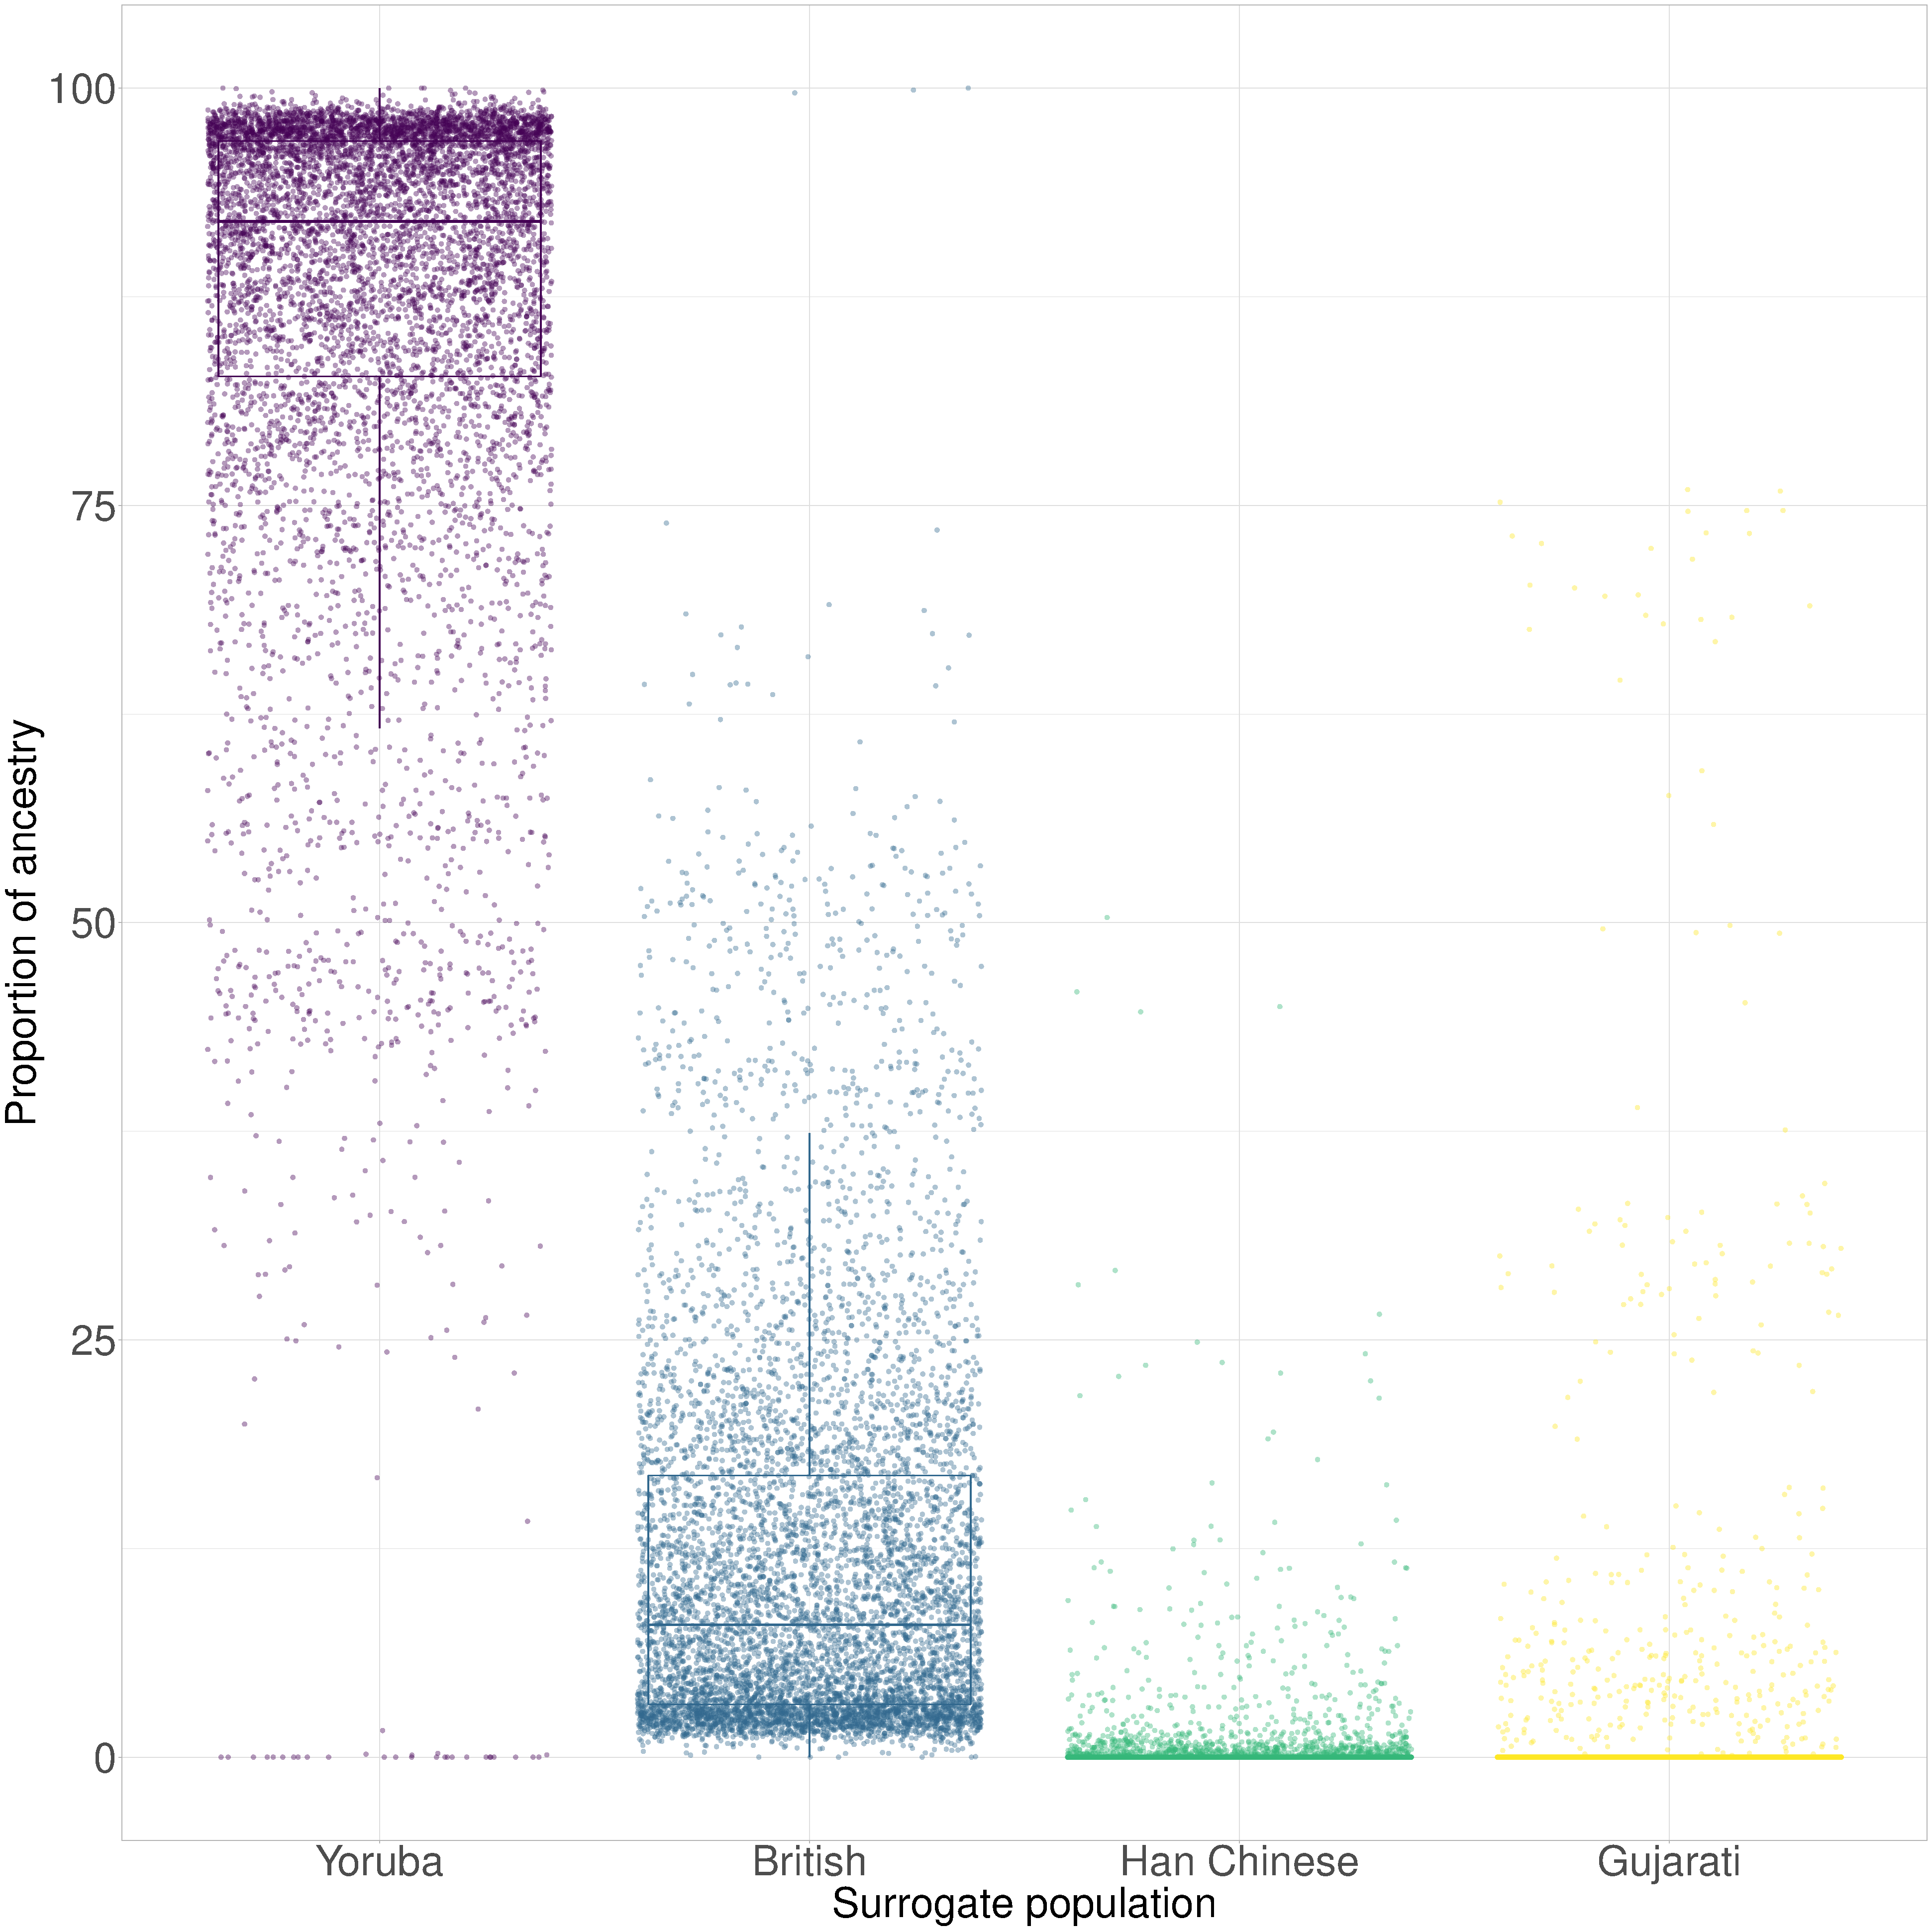
\includegraphics[width=1.0\textwidth]{../images/chapter3/African_Inds_proportions.pdf}
    \caption{Ancestry proportions inferred from supervised ADMIXTURE run (k=4) for all individuals who self identified as being either "Caribbean", "African" or "Black or Black British". Points within each column are given random jitter to improve visual clarity.}
    \label{fig:African_Inds_proportions_ADMIXTURE}
\end{figure}

\subsection{To impute or not?}

In order to use the Human Origins dataset as a reference in ChromoPainter analysis to ancestry in U.K. Biobank individuals, the datasets must be merged. The overlap of SNPs genotyped in each dataset is only 70,776 SNPS, or an average of $\approx$1 SNP per 40Kb. Given linkage disequilibrium (e.g.\ as measured by Pearson's correlation) between pairs of SNPs decays to background levels by 100Kb within most populations \cite{bosch2009decay}, analysing 70,000 SNPs may substantially decrease any potential power gains from modeling haplotypes to detect fine-scale differences between populations. In contrast, the imputed U.K. Biobank dataset has 535,544 SNPs in total, all of which are genotyped in the Human Origins reference dataset and 87.7\% of which are imputed in UK Biobank individuals. While this may boost power over using only 70,000 SNPs, including a high percentage of imputed SNPs may bias ancestry inference. Therefore, I needed to determine a) whether there is a loss of power when 70,000 SNPs relative to the a full 500,000 SNP dataset and b) whether there is bias when using a dataset which contains a majority of imputed SNPs.  

To answer these questions, I returned to the imputed and unimputed Human Origins datasets I describe in Section \ref{sec:ImputationBiasTest}. Recall here I reduced the Human Origins dataset to 70K SNPs and then imputed to approximately 500,000 SNPs using HRC and therefore determine whether using the imputed or the 70,000 SNP Human Origins dataset is better in this scenario, I performed a painting using (i) the full 560,442 genotyped SNPs, (ii) only the 64,762 genotyped SNPs overlapping UK Biobank, and (iii) 500,000 SNPs that include the 64.47K genotyped SNPs and 430,000 SNPs imputed using the HRC reference. I performed painting (ii) in both linked and unlinked mode to determine whether there is any haplotype information using 70,000 SNPs.

For each of the three datasets described above, I selected all ethnic groups from Nigeria, Cameroon and Ghana which had five or more individuals (n=51 populations, n=1203 individuals) and split each population randomly in half, into `donors' and `recipients'. I painted all recipient populations (n=51) using all donor populations (n=51) using a leave-one-out approach (description and motivation of this approach given in Appendix section \ref{sec:leave_one_out}). I only considered populations of five individuals or more because any fewer individuals would likely result in very weak power to assign individuals to that population. I tested the information content of each painting by counting how often individuals copy more from individuals in their own populations than individuals from other populations. I also counted the number of times a population had the lowest TVD (motivation and description of TVD given in Appendix section \ref{sec:appendixTVD}) with the mean copyvector of all other individuals in its own population (Table \ref{table:TVD_copying}).

Populations in the 70,000 non-imputed painting matched more to and had a lower $TVD$ with their own mean population copyvector than the 500,000 non-imputed painting. Whilst it seems counter-intuitive that there is more power using a smaller number of SNPS, this is broadly consistent with my previous findings in Chapter 2, which showed that metrics of painting information plateau (Fig. \ref{fig:Devon_Cornwall_TVD_reduced_assignment}) (i.e.\ there is no clear benefit to using more than 50,000 SNPs in terms of assigning individuals to a population). This is reassuring and suggests there is no loss of power when using the 70,000 SNP set. This data also shows that there is a fairly dramatic loss of power when using imputed data relative to non-imputed data, as over 3x the number of populations had a lower TVD with their own population when using imputed compared to non-imputed data.

\begin{table}
\centering
\small
\begin{tabular}{l|l|l}
\toprule
painting & TVD & copying\\
\midrule
70K (linked) & 44\% & 24\%\\
70K (unlinked) & 20\% & 17\%\\
imputed (linked) & 14\% & 14\%\\
full (linked) & 38\% & 23\%\\
\bottomrule
\end{tabular}
\caption{Percentage of populations which had lowest TVD (TVD) or copied the most (copying) from their own population under different paintings. 70K linked used 70,000 SNPs in linked mode, 70K used 70,000 SNPs in unlinked mode, imputed used 430,000 imputed and 70,000 non-imputed SNPs in linked mode and full used 500,000 non-imputed SNPs in linked mode.}
\label{table:TVD_copying}
\end{table}

Given the above results suggested that imputing data results in a loss of information, I was interested in whether this constituted a `bias' towards certain populations. Reference-based imputation methods rely on identifying reference haplotypes which are closest to the target haplotypes. However, if the ethnic groups that the target individuals derive ancestry from are not present in the imputation reference panel, missing variants are imputed from populations in the reference panel which are most closely related to the target samples. In this case, two target populations may be imputed to appear more genetically similar to that reference population, reducing the differentiation between them (Fig \ref{fig:imputed_nonimputed_donation}). In theory, this artificial similarity would be propagated through to the ChromoPainter analysis. In particular, we would expect populations present in the reference panel to donate more to all other individuals than they would if no imputation had taken place.  

For example, in the case of the Haplotype Reference Consortium, the closest reference population to two African target samples from e.g. Cameroon may be the Yoruba from Nigeria, which is one of the few west African groups in the reference. These samples would appear more similar to the Yoruba ethnic group than if they had not been imputed. In a ChromoPainter analysis, the Yoruba donor population would donate more than than when using non-imputed SNPs.    

Comparing the imputed and non-imputed coancestry matrices revealed biases consistent with the above expectation. If the coancestry matrix columns are combined into populations, then the sum of each column gives the total length of genome that population contributes to all recipient individuals in the dataset. Therefore, comparing the column sums between the imputed and non-imputed matrices informs us about which populations contribute more when using imputed compared to non-imputed SNPs. Fig \ref{fig:imputed_excess_copying_pops} shows the amount of differential haplotype donation on a per-population basis, with populations highlighted based on their presence or absence in the 1000 genomes dataset. It is clear that populations present in the 1000 genomes are primarily clustered towards the right hand side, rather than randomly distributed across figure. This strongly suggests that imputation causes a bias towards those populations present in a reference panel. 

To formally test whether the ordering of populations was likely significantly different to the ordering expected under the null model of no impact of being present in the 1000 genomes dataset, I performed a non-parametric permutation test. If we order the populations based on their differential haplotype donation and assign a rank value to each population, we can calculate the sum, $S$ of the ranks values of all populations present in the 1000 genomes. If the 1000 genomes populations are clustered at the higher end of the ordering, we would expect the value of $S$ to be smaller than if the populations are randomly distributed across the ordering. I performed 100,000 replications of randomly ordering the population labels and calculating the value of $S$. Of the 100,000, 26 had $S$ greater than the true empirical value calculated from the data, showing the ordering of the populations is unlikely to be due to chance ($p=0.00026$). This permutation test was motivated by the Wilcoxon Rank Sum Test.  

\begin{sidewaysfigure}
	    \centering
	    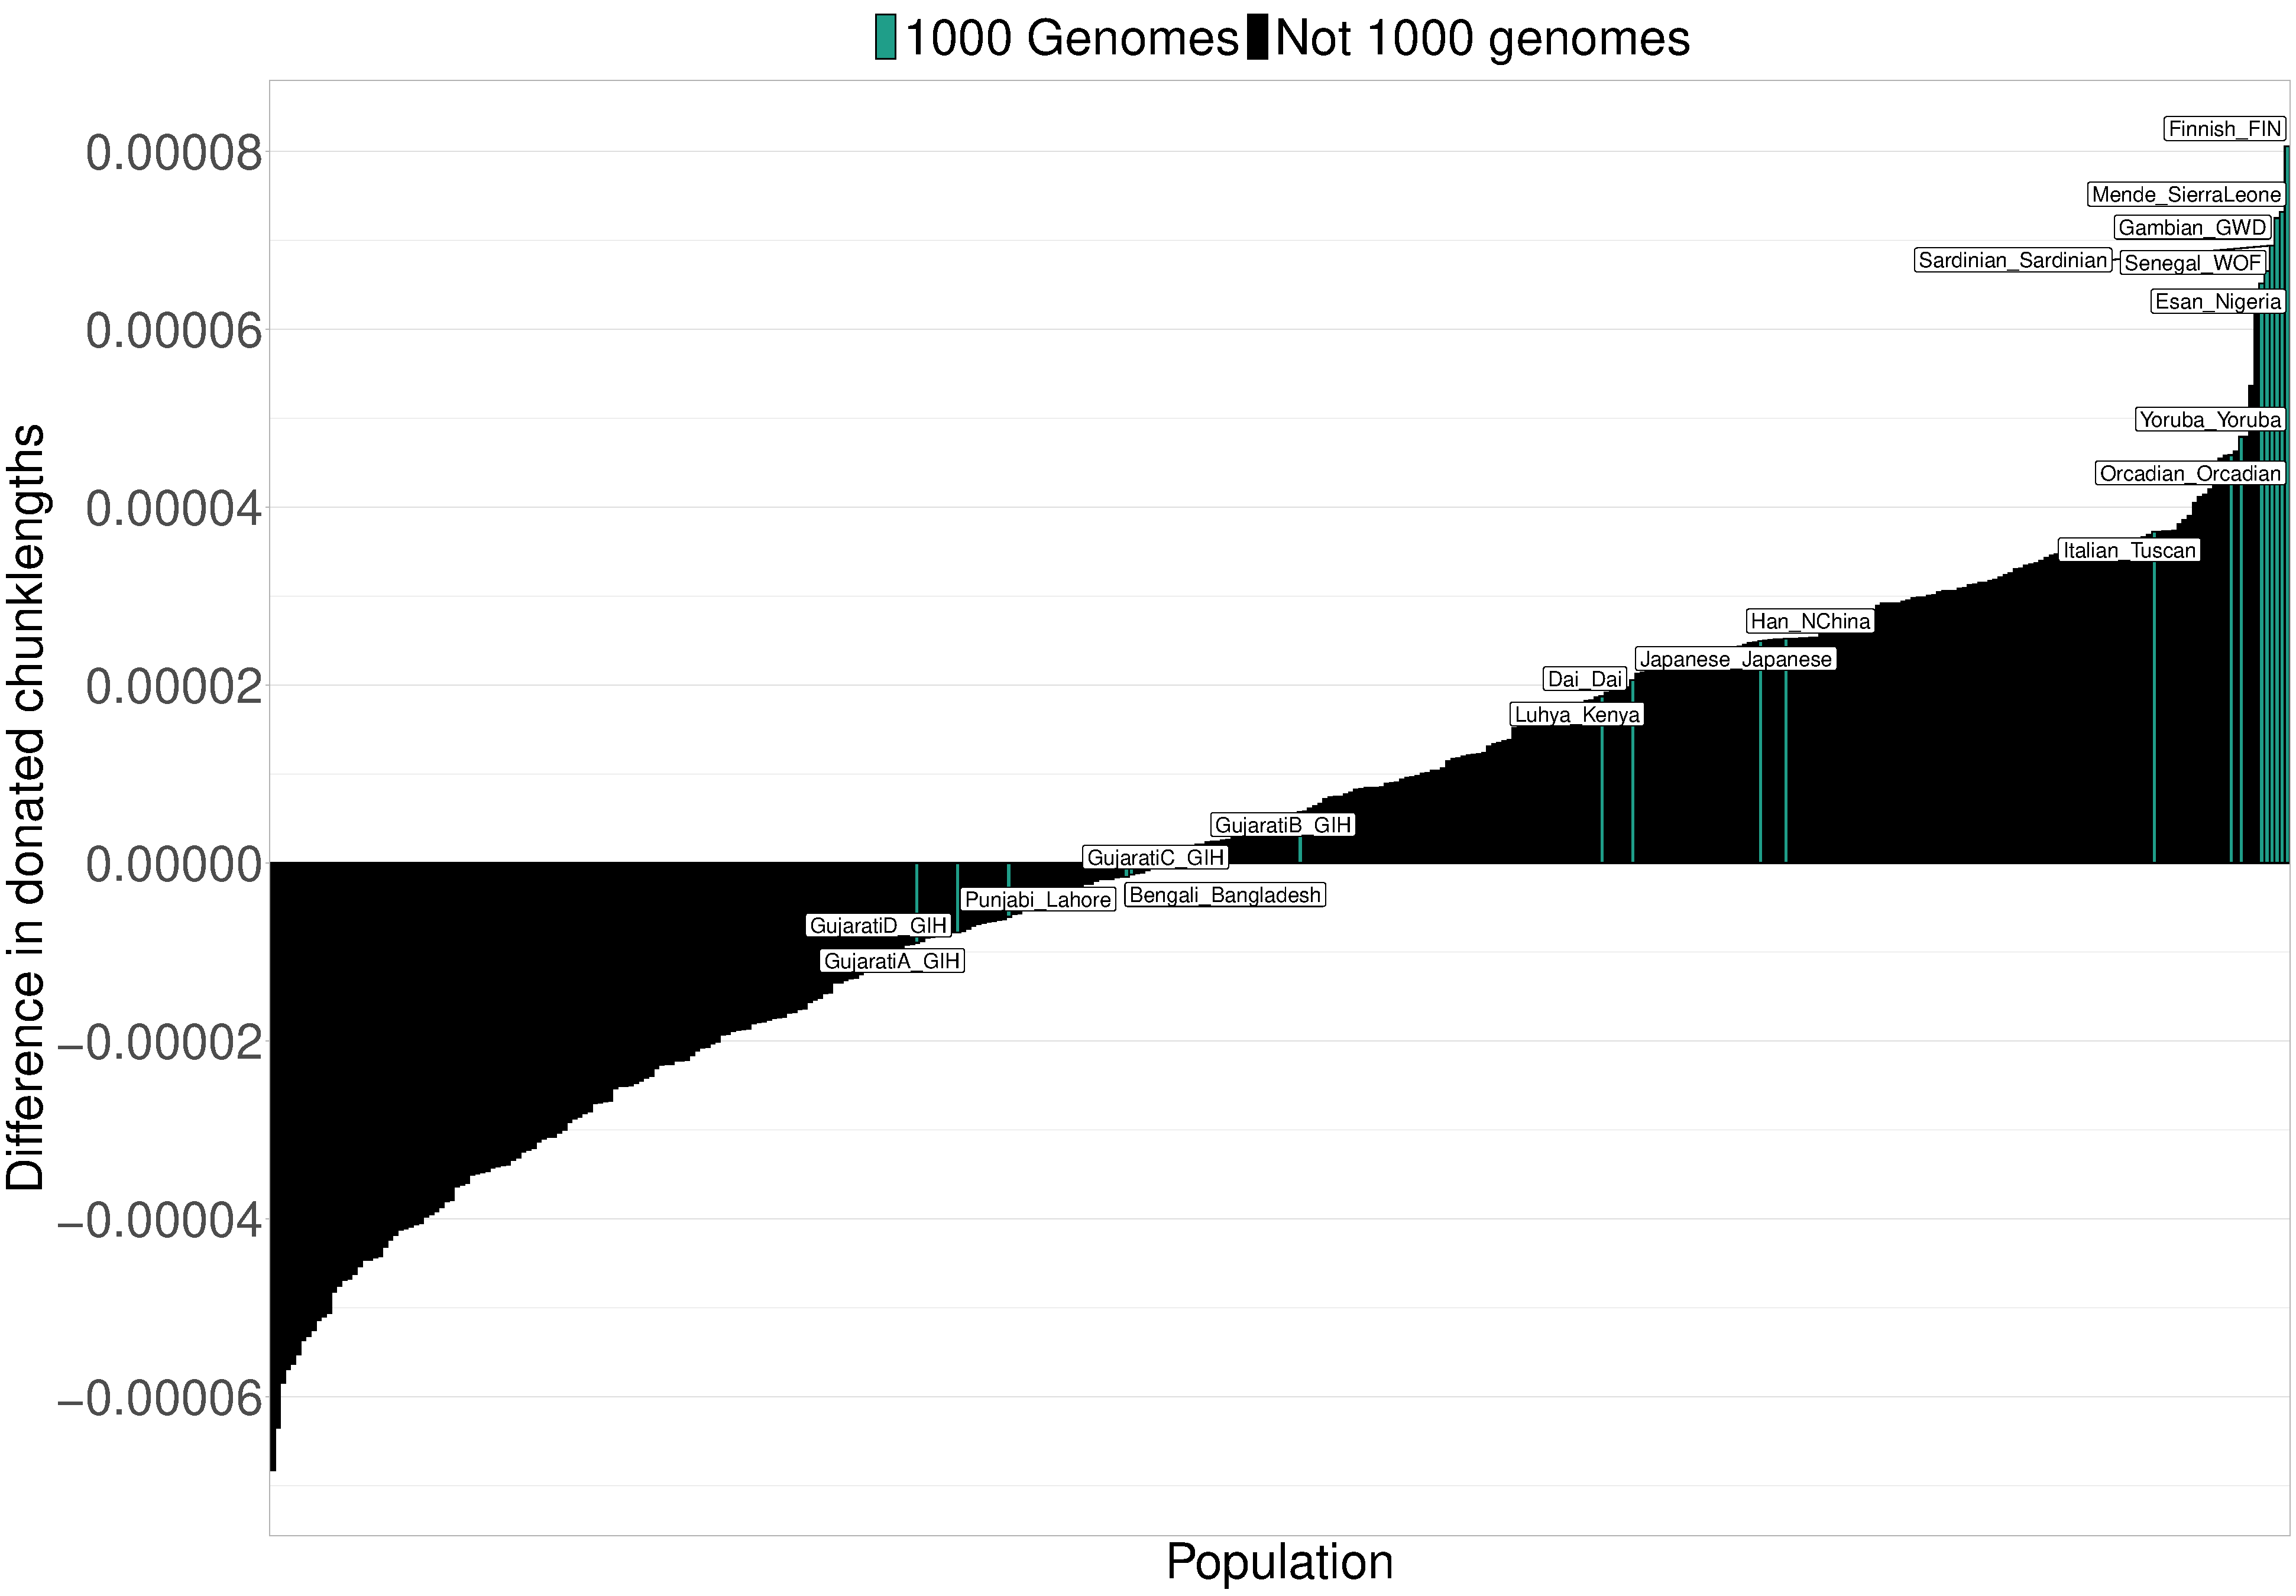
\includegraphics[width=1.0\textwidth]{../images/chapter3/imputed_excess_copying_pops.pdf}
	    \caption{Differences in the amount donated by populations when using imputed and non-imputed data. Each vertical bar corresponds to a single population (N=395), with the height of the bar corresponding to the difference in haplotype donation, with positive values indicating increased donation and negative values indicating reduced donation. Bars coloured in green are also present in the 1000 genomes imputation panel and black bars are not present in the 1000 genomes.}
	    \label{fig:imputed_excess_copying_pops}
\end{sidewaysfigure}

Put together, these results suggest that using imputed data would introduce a level of bias and loss of information. Therefore, in all later analysis, I chose to use the approximately 70,000 non-imputed SNPs which overlap between the Human Origins and U.K. Biobank datasets. 

\subsection{African ancestry in the U.K. Biobank samples is concentrated in Ghana and Nigeria}

Using approximately 70,000 directly genotyped SNPS, I painted all U.K. Biobank individuals with at least 50\% African ancestry (n=8475) using all Human Origins individuals as donors (n=5,577).

Principal component analysis on the resulting chunkcounts coancestry matrix reveals the general structure of the selected individuals, alongside the reference populations (Fig. \ref{fig:PCA_chunklengths_HumanOrigins_U.K.Biobank}). Three clines are present; one of similarity to Southern African populations typified by the Zulu ethnic group from South Africa, one of similarity to West African populations such as Yoruba and Cameroon\_Dii, and the last to East African populations such as those from Ethiopia. The majority of U.K. Biobank individuals are positioned near West African populations; in particular between Yoruba and Cameroon\_Arabe. The presence of a broad cluster of West African individuals is consistent with prior expectations that West African ancestry should be prevalent in a sample of British individuals, due to the history of migration from this region \cite{banton1953recent}. A second cluster of UK Biobank individuals is located along the Southern African cline, close to the Bantu\_SA label. 

\begin{figure}[htp]
    \centering
    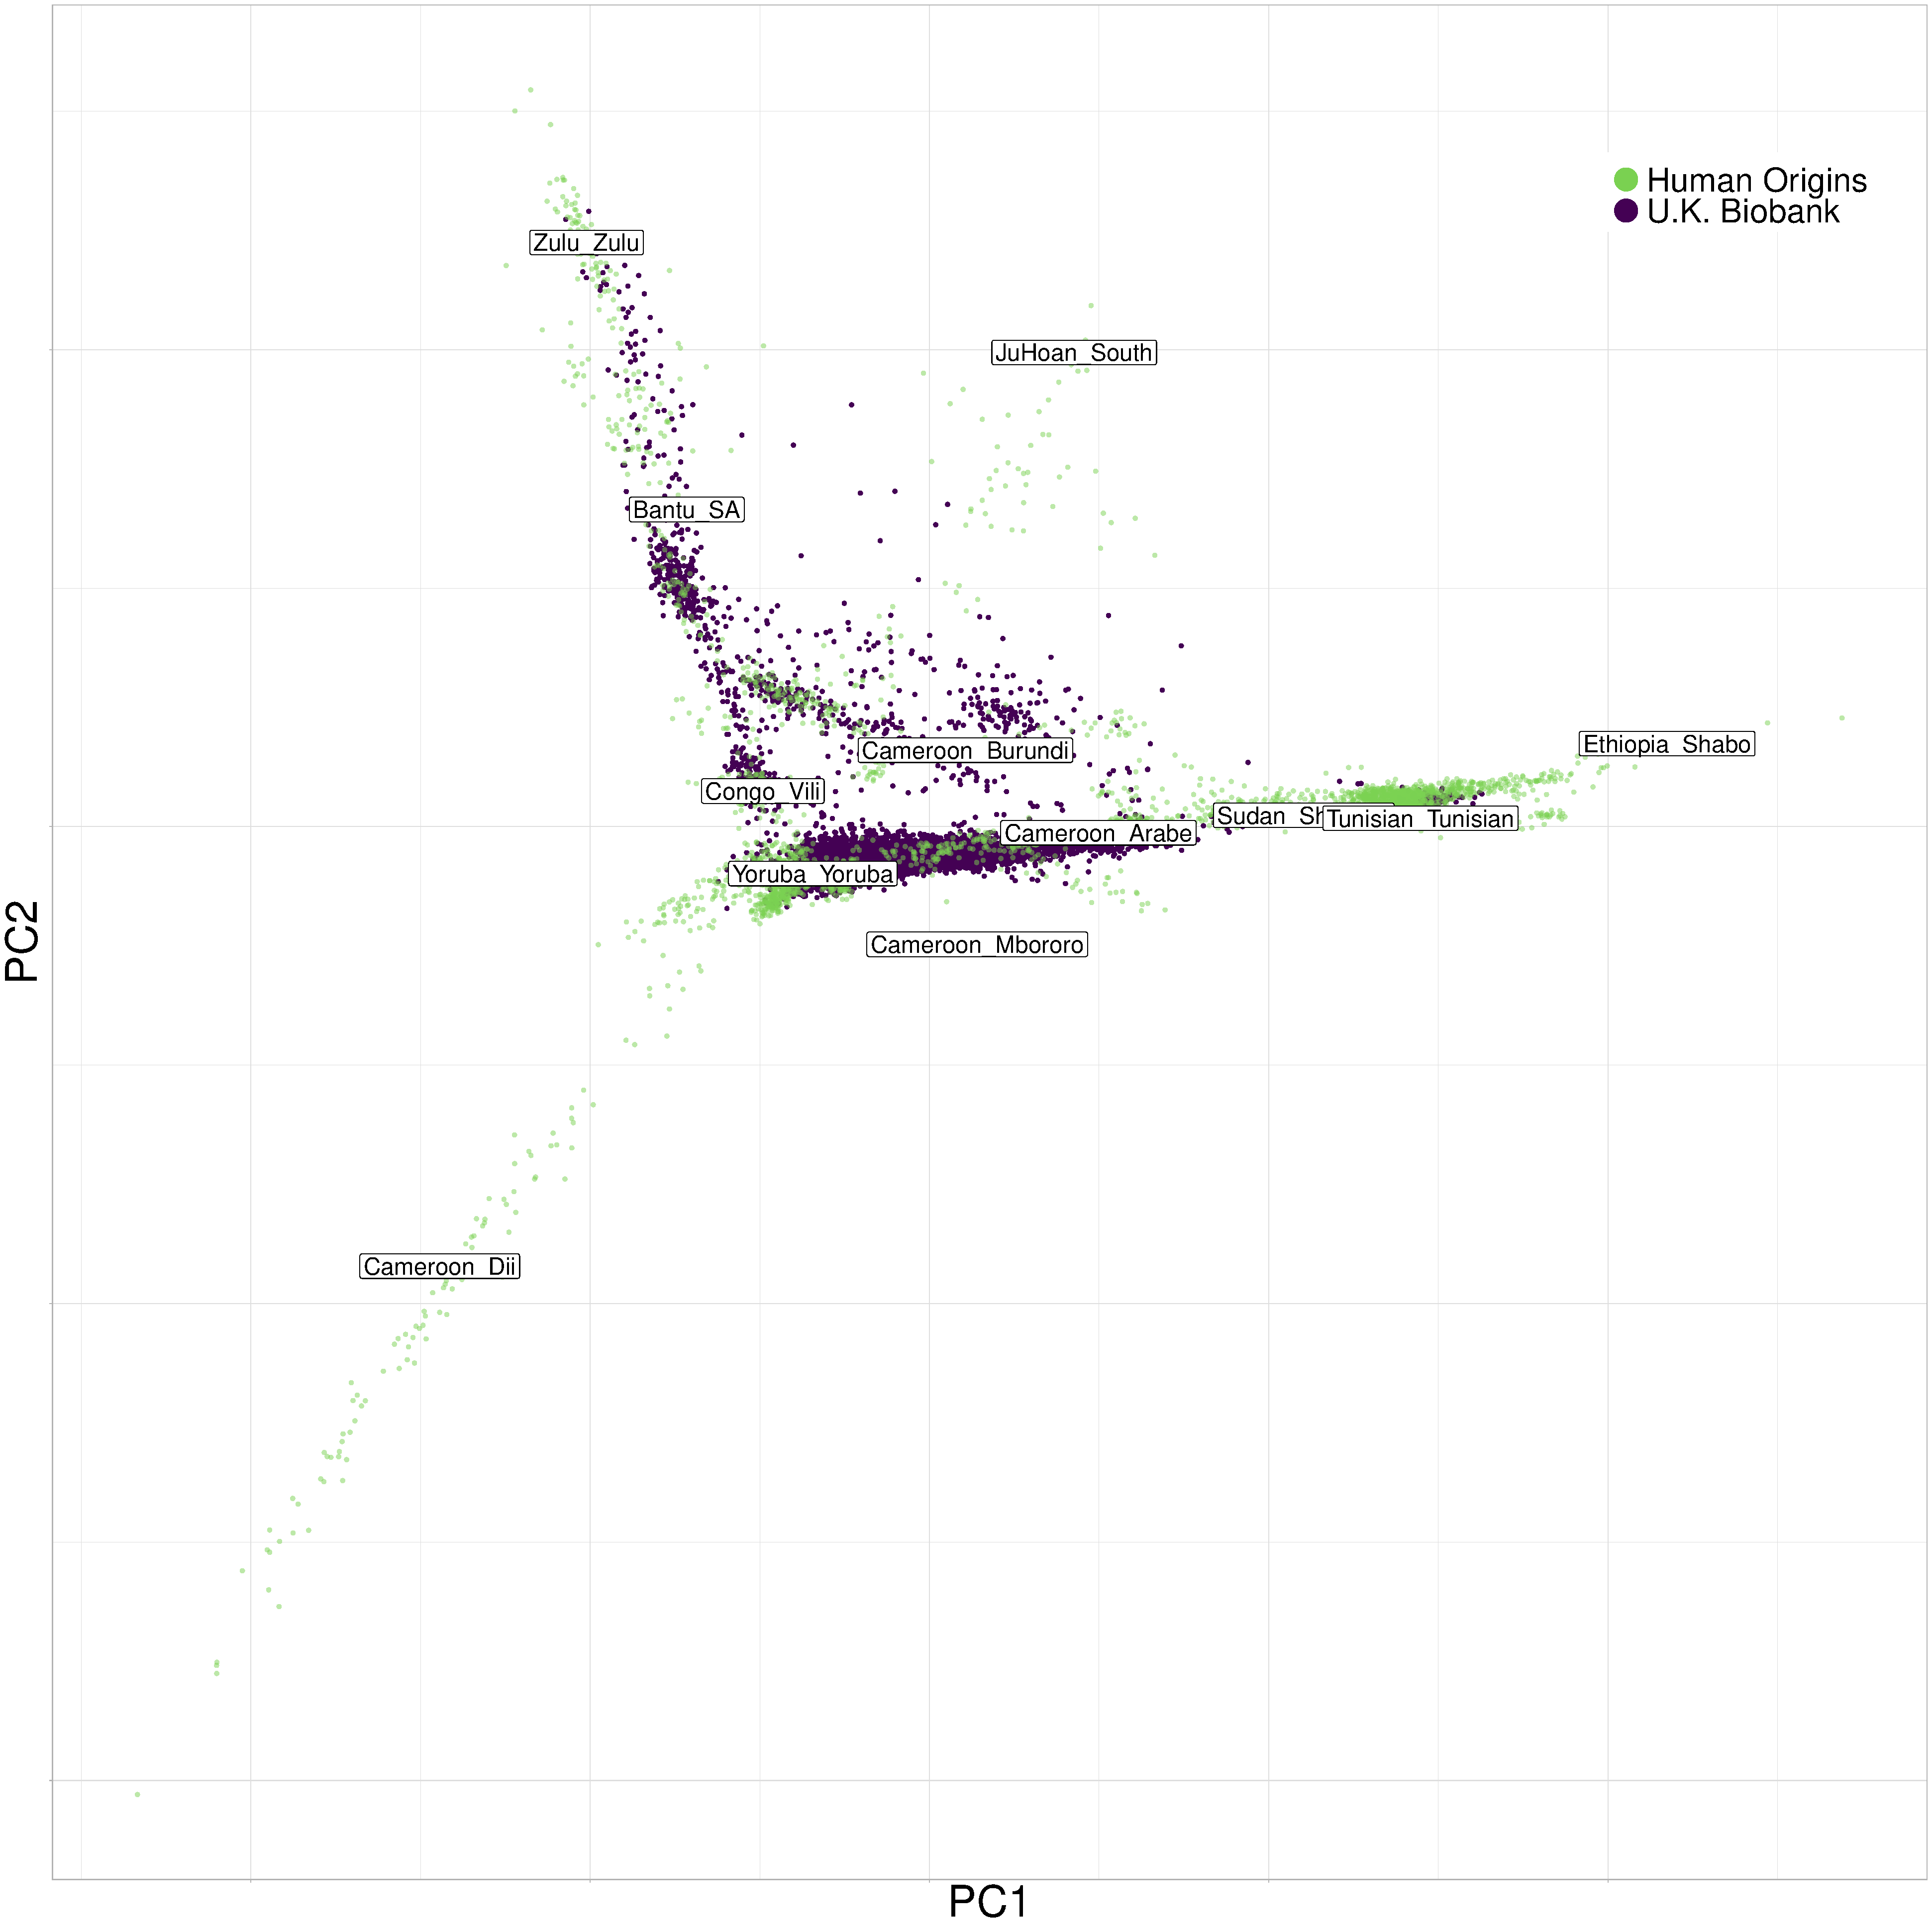
\includegraphics[width=1.0\textwidth]{../images/chapter3/ChromoPainter_PCA_UKB_HO.pdf}
    \caption{Principle component analysis of chunklengths matrix for U.K. Biobank individuals with $\geq$50\% inferred recent African ancestry and human origins array. Individuals are coloured dependent on whether they are U.K. Biobank (green) or Human Origins (purple) samples. Labels indicate mean principle component coordinates for individuals in that population. A random sample of populations were chosen to have labels to prevent the figure from being too cluttered.}
    \label{fig:PCA_chunklengths_HumanOrigins_U.K.Biobank}
\end{figure}

Aggregating the columns of the coancestry matrix by reference population and taking the sum of each column gives the total length of genome for which a U.K. Biobank individual shares recent ancestry with individuals from that donor population. This can be visualised on a map, where each point represents a reference population and the colour corresponds to the total amount that reference population contributes towards the ancestry of all retained U.K. Biobank individuals (Fig. \ref{fig:haplotype_sharing_map_zoomed_II}). Higher values correspond to more ancestry from that population in the U.K. Biobank sample. However, it should be noted that raw ChromoPainter output can be influenced strongly by sample size and so the values shown in Fig. \ref{fig:haplotype_sharing_map_zoomed_II} should not be taken literally as an exact reflection of the ancestry distribution.

\begin{figure}[htp]
    \centering
    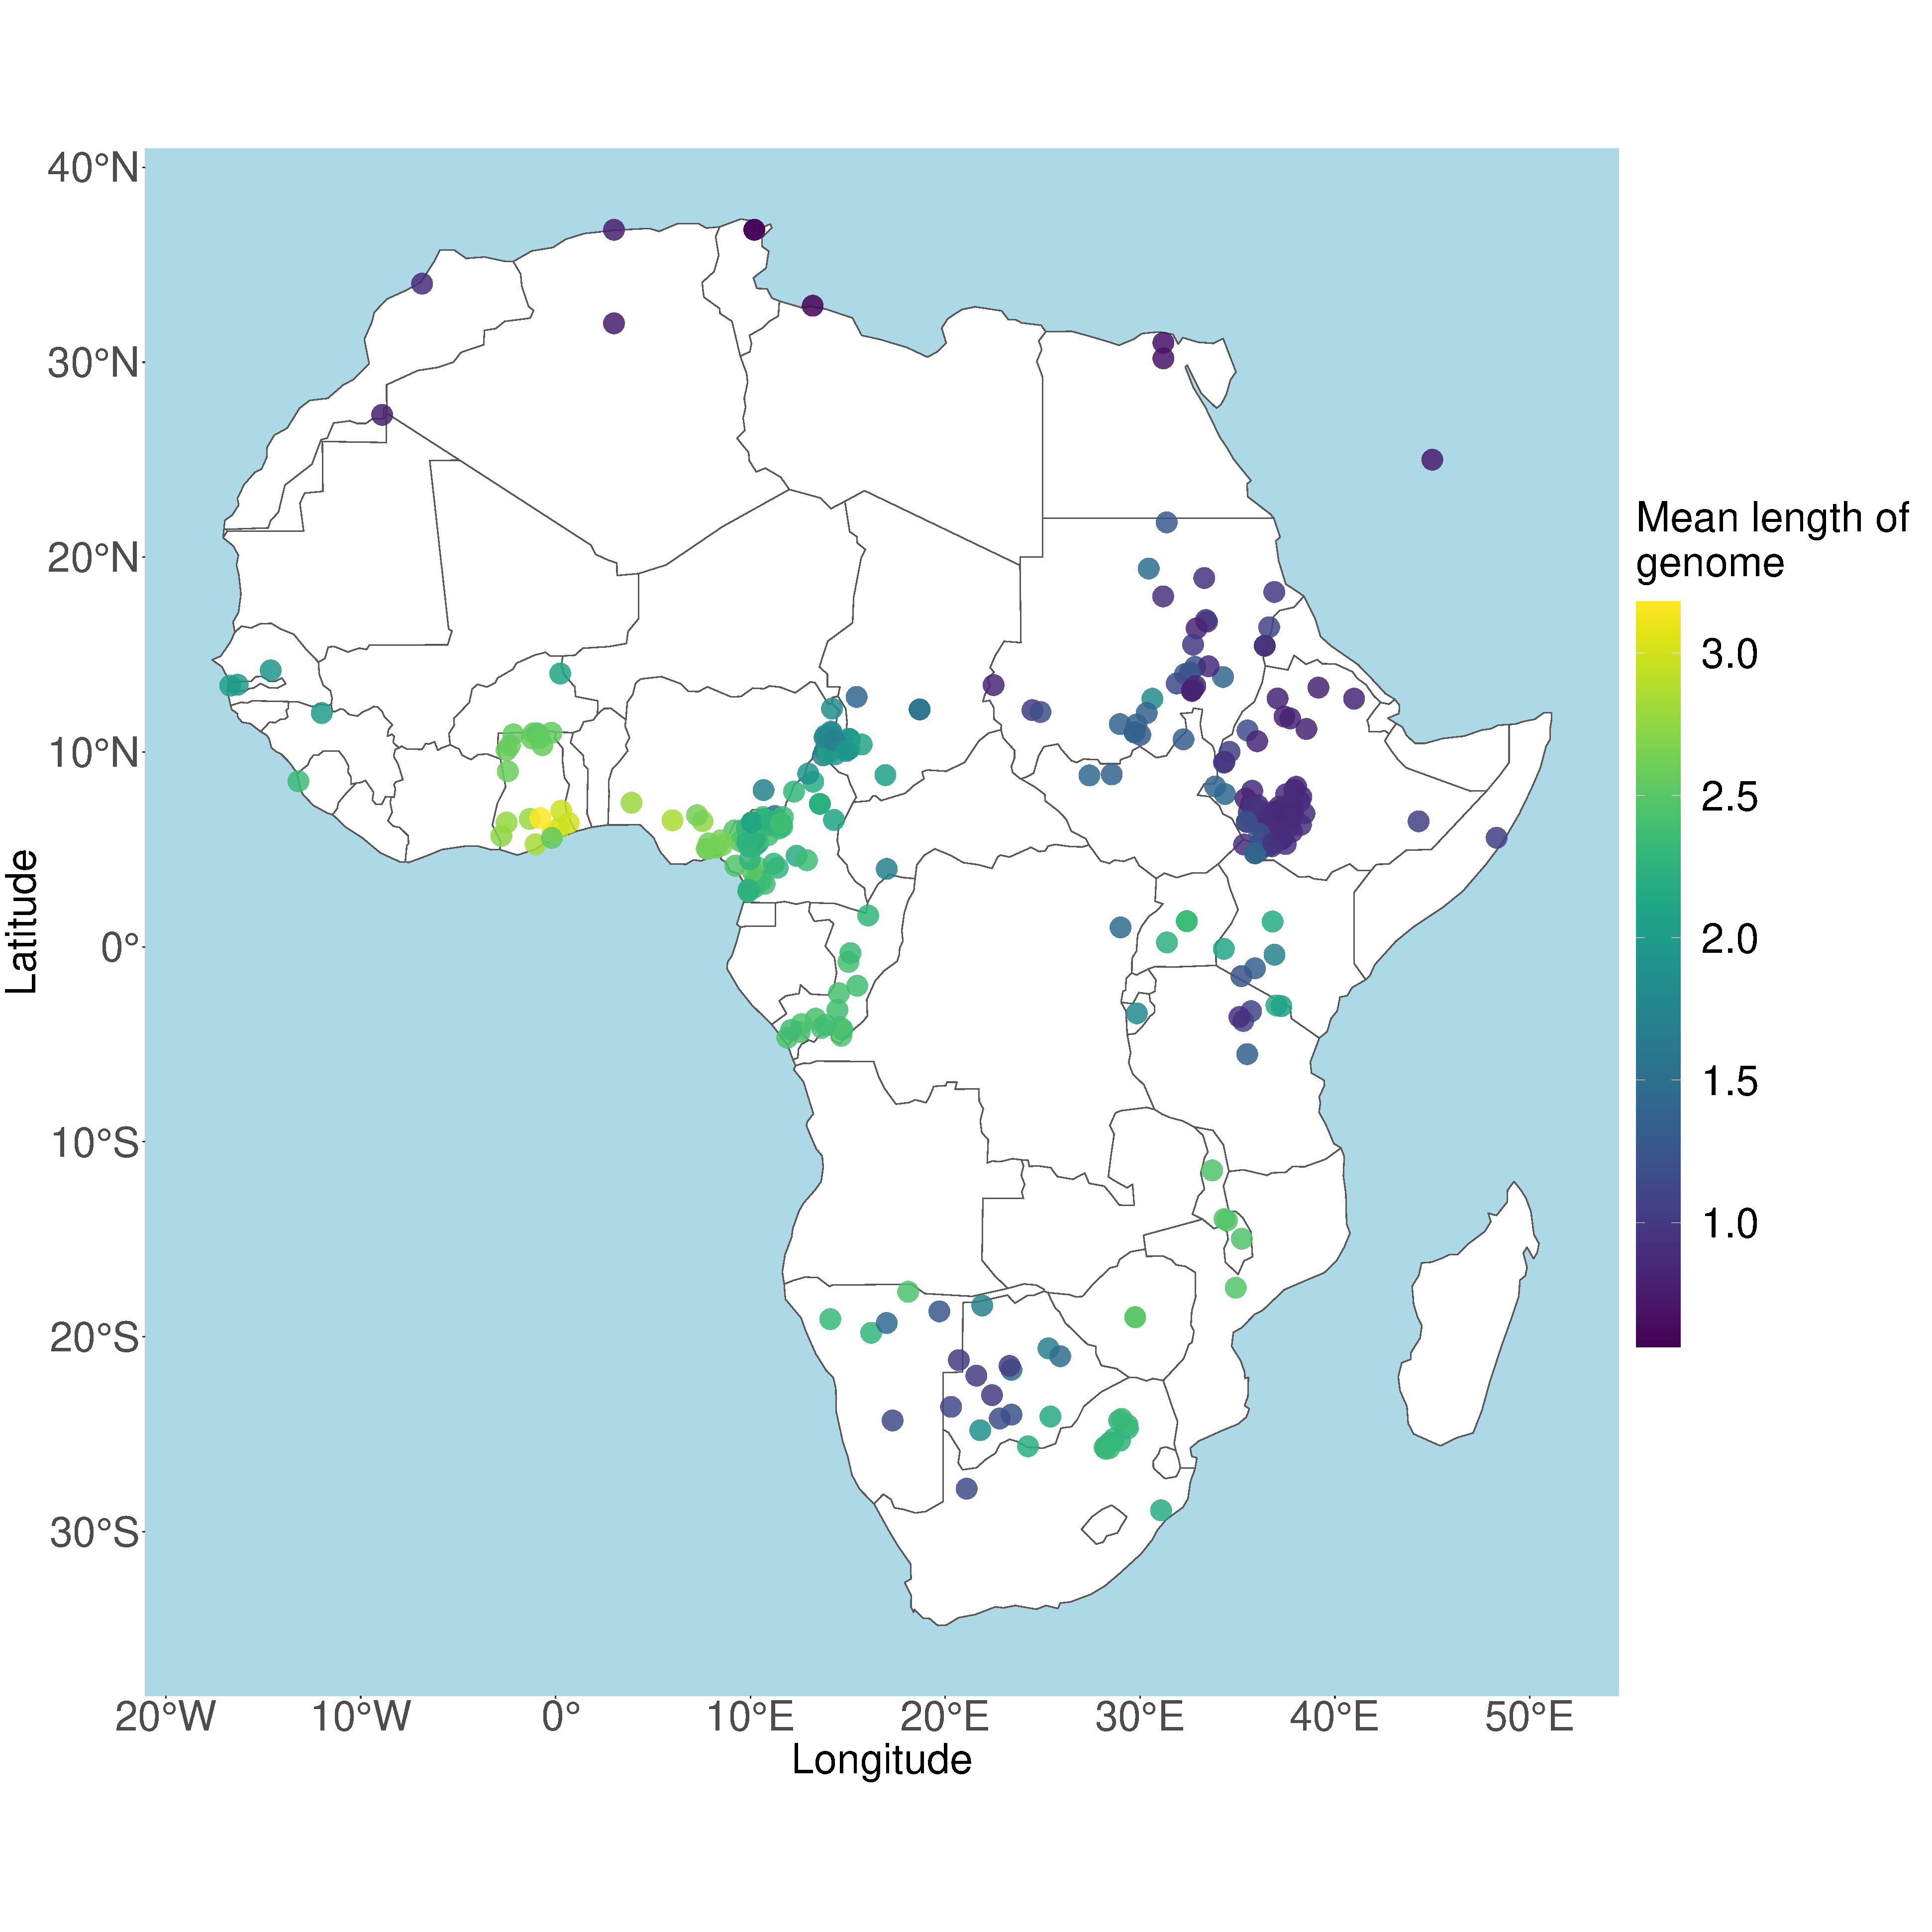
\includegraphics[width=1.0\textwidth]{../images/chapter3/haplotype_sharing_map.pdf}
    \caption{Map of haplotype donation to U.K. Biobank individuals. Each point represents a different African population. Colour corresponds to the mean length (cM) that populatation donated to all African U.K. Biobank individuals.}
    \label{fig:haplotype_sharing_map_zoomed_II}
\end{figure}

The map supports the findings from the PCA in Fig. \ref{fig:PCA_chunklengths_HumanOrigins_U.K.Biobank}; the populations with the largest contribution are those from West Africa (Fig. \ref{fig:haplotype_sharing_map_zoomed_II}). In particular, populations from Ghana and Nigeria contribute the most to the ancestry of Biobank individuals. On the other hand, populations in east and north Africa contribute relatively little, with southern / south-east Africa being approximately intermediate. This is consistent with two different historical events. 

Firstly, it is known from historical and genetic studies that a majority of the individuals who were forcibly transported from Africa to the Americas during the transatlantic slave trade were from the west coast of Africa \cite{micheletti2020genetic}. Given the U.K. Biobank sample contains many individuals who were either born in, or trace their ancestry from the Caribbean, a region that had a large influx of slaves \cite{rawley2005transatlantic}, we would expect there to be a large contribution of ancestry from west Africa. Secondly and more recently, there has been a relatively large amount of historical immigration from countries in west Africa, such as Ghana and Nigeria, to the U.K \cite{banton1953recent}. Although there are a number of immigrants from other parts of Africa, reflected in the non-zero contributions from other ethnic groups, these contributions are small compared to those from West Africa.

I performed the same visualisation using the painting using imputed SNPs and the ancestry distribution was qualitatively the same. 

I used SOURCEFIND to infer the proportion of ancestry that each UK Biobank individual shares most recently with each of the 535 surrogate groups, as this accounts for uneven donor population sizes. A map of proportions is given in Fig. \ref{fig:SF_props_map}, with each point corresponding to the mean percentage of ancestry of that particular group across all African U.K. Biobank individuals. Similar to the copyvector map, the ancestry is focused around Nigeria and Ghana, with Yoruba (39.8\%) and Ghana Fante (7.31\%) having the highest mean proportions. The distribution of colour on this figure is focused around a smaller number of populations compared to Fig. \ref{fig:haplotype_sharing_map_zoomed_II}. This is because SOURCEFIND attempts to narrow down the set of populations which most likely contribute towards the ancestry of a given individual and so appear `cleaner' than raw ChromoPainter results. 

\begin{figure}[htp]
    \centering
    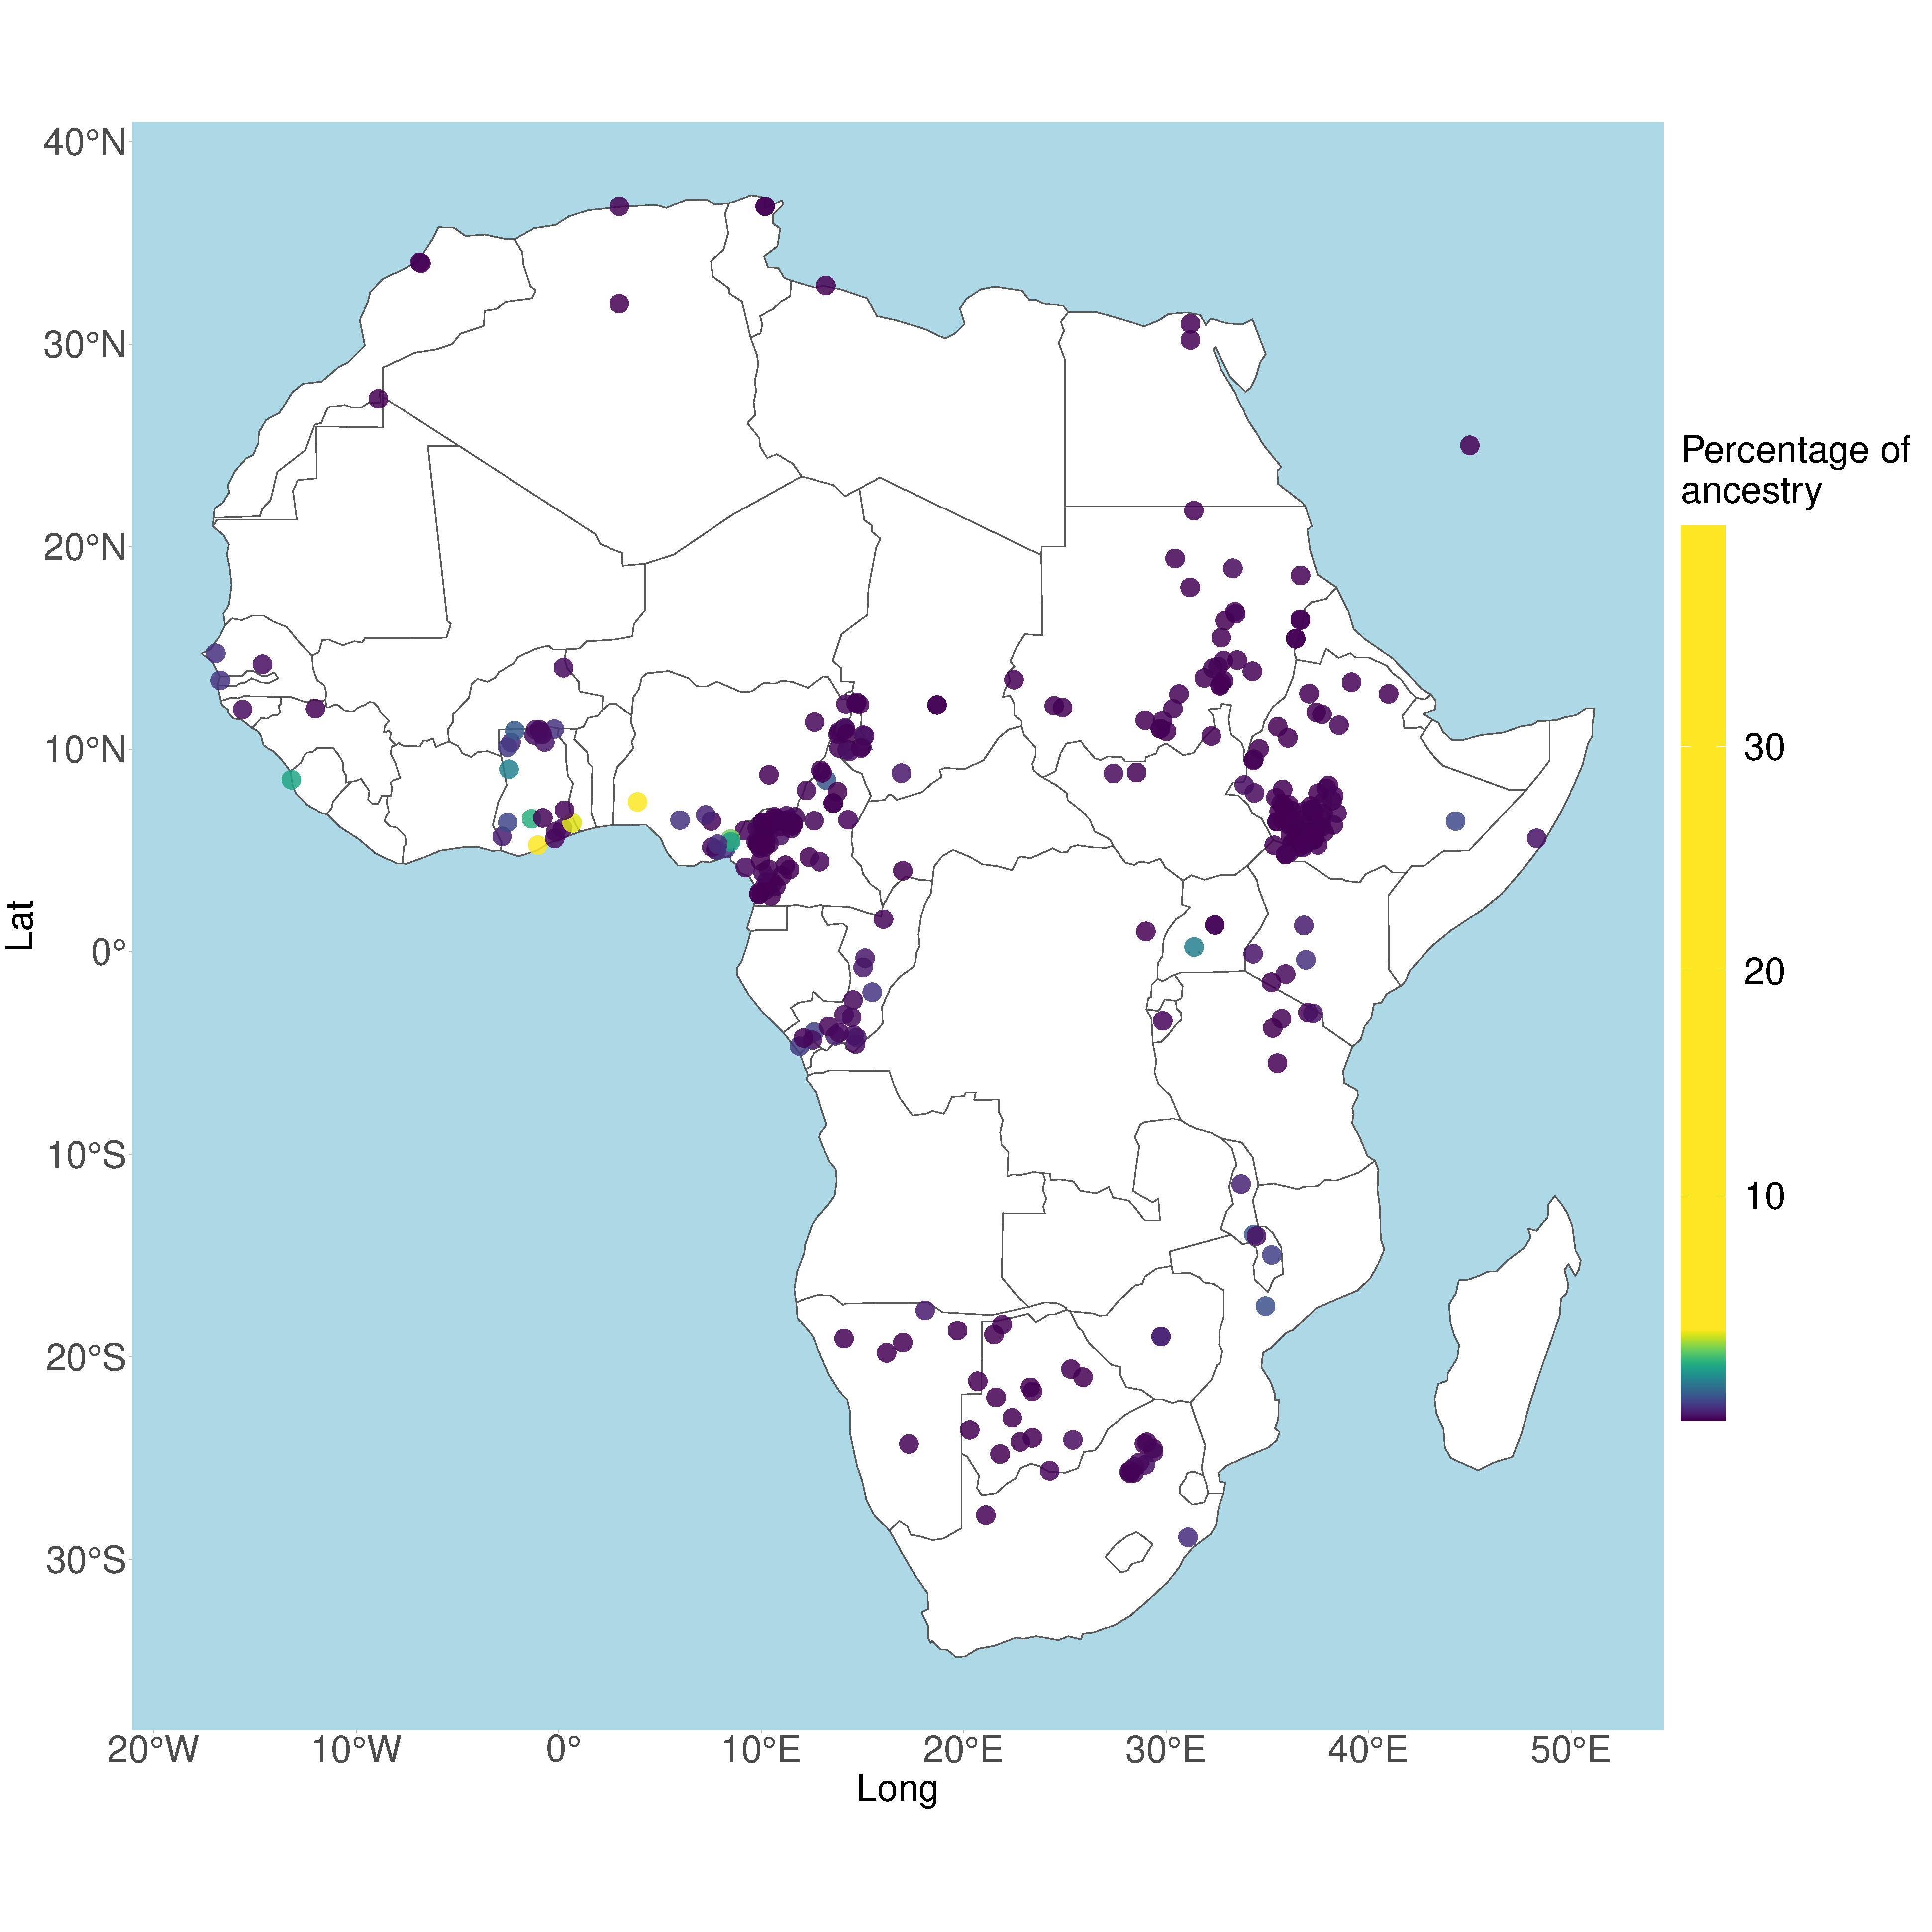
\includegraphics[width=1.0\textwidth]{../images/chapter3/SF_props_map.pdf}
    \caption{Map displaying the mean proportion of SOURCEFIND estimated ancestry of each African reference population within U.K. Biobank individuals. Each point is an African reference population with the colour corresponding to the mean ancestry proportion for that population across selected U.K. Biobank individuals. The colour-bar has been rescaled as two populations, Yoruba and Ghana\_Fante have substantially higher proportions than all other populations.} 
    \label{fig:SF_props_map}
\end{figure}


Fig. \ref{fig:SF_props_distribution_top30} displays the 30 ethnic groups with the highest mean proportions of ancestry within the U.K. Biobank individuals, and the distribution of values within each group. Yoruba was a clear standout for the most represented population;  3604/8309 individuals had at least 50\% Yoruba ancestry. This is compared to the next most common ancestry, Ghana\_Fante, which had an average of 7.3\% per person and 373/8309 individuals with at least 50\% ancestry. It is not clear what the reason for the large amount of Yoruban ancestry relative to all other populations is. One possible answer may come from considering the birth country of the U.K. participants. Of all the individuals for which we have country of birth data for (n=6190), more of them were born in the Caribbean (n=2263) relative to any other country. This should not be surprising given the history of migration from the Caribbean to the U.K. Of the individuals born in the Caribbean, over half were assigned to the Yoruban ethnicity, a much higher proportion than any other country of birth. Therefore, one could tentatively explain the abundance of Yoruba ancestry as resulting from the transatlantic Slave Trade, where individuals from the Yoruba ethnic group were taken to the Caribbean at a higher frequency than other nearby ethnic groups in the Human Origins reference. This may be in part because Yoruba is the second largest ethnic group in Nigeria and individuals belonging to it live primarily in coastal areas where the Slave Trade operated. The relatively large number of individuals from the Caribbean in the U.K. could thus have brought Yoruban ancestry to the U.K. 

\begin{figure}[htp]
    \centering
    \includegraphics[width=1.0\textwidth]{../images/chapter3/SF_props_distribution_top30.pdf}
    \caption{The 30 Human Origins populations which have the highest contribution to all U.K. Biobank individuals with at least 50\% African Ancestry, based on SOURCEFIND analysis. Each row of points contains 8476 individuals and their position corresponds to the percentage of ancestry from that population. }
    \label{fig:SF_props_distribution_top30}
\end{figure}

There are other instances of an over and under-representation of one ethnic group from a particular country (Fig. \ref{fig:all_countries_SF_props_pie_chart}). For example, Nigeria is dominated by a single ethnic group, despite having data for 31 different ethnic groups.  On the other hand, the individuals from Sudan are more evenly distributed across ethnicities. This may be caused because there are more reference ethnic groups in Sudan to assign individuals to. Further, it is known (personal communication N.Bird, 2021) that using the Human Origins dataset, there is inability to distinguish  between individuals in closely related Sudanese populations. 

\begin{figure}[htp]
    \centering
    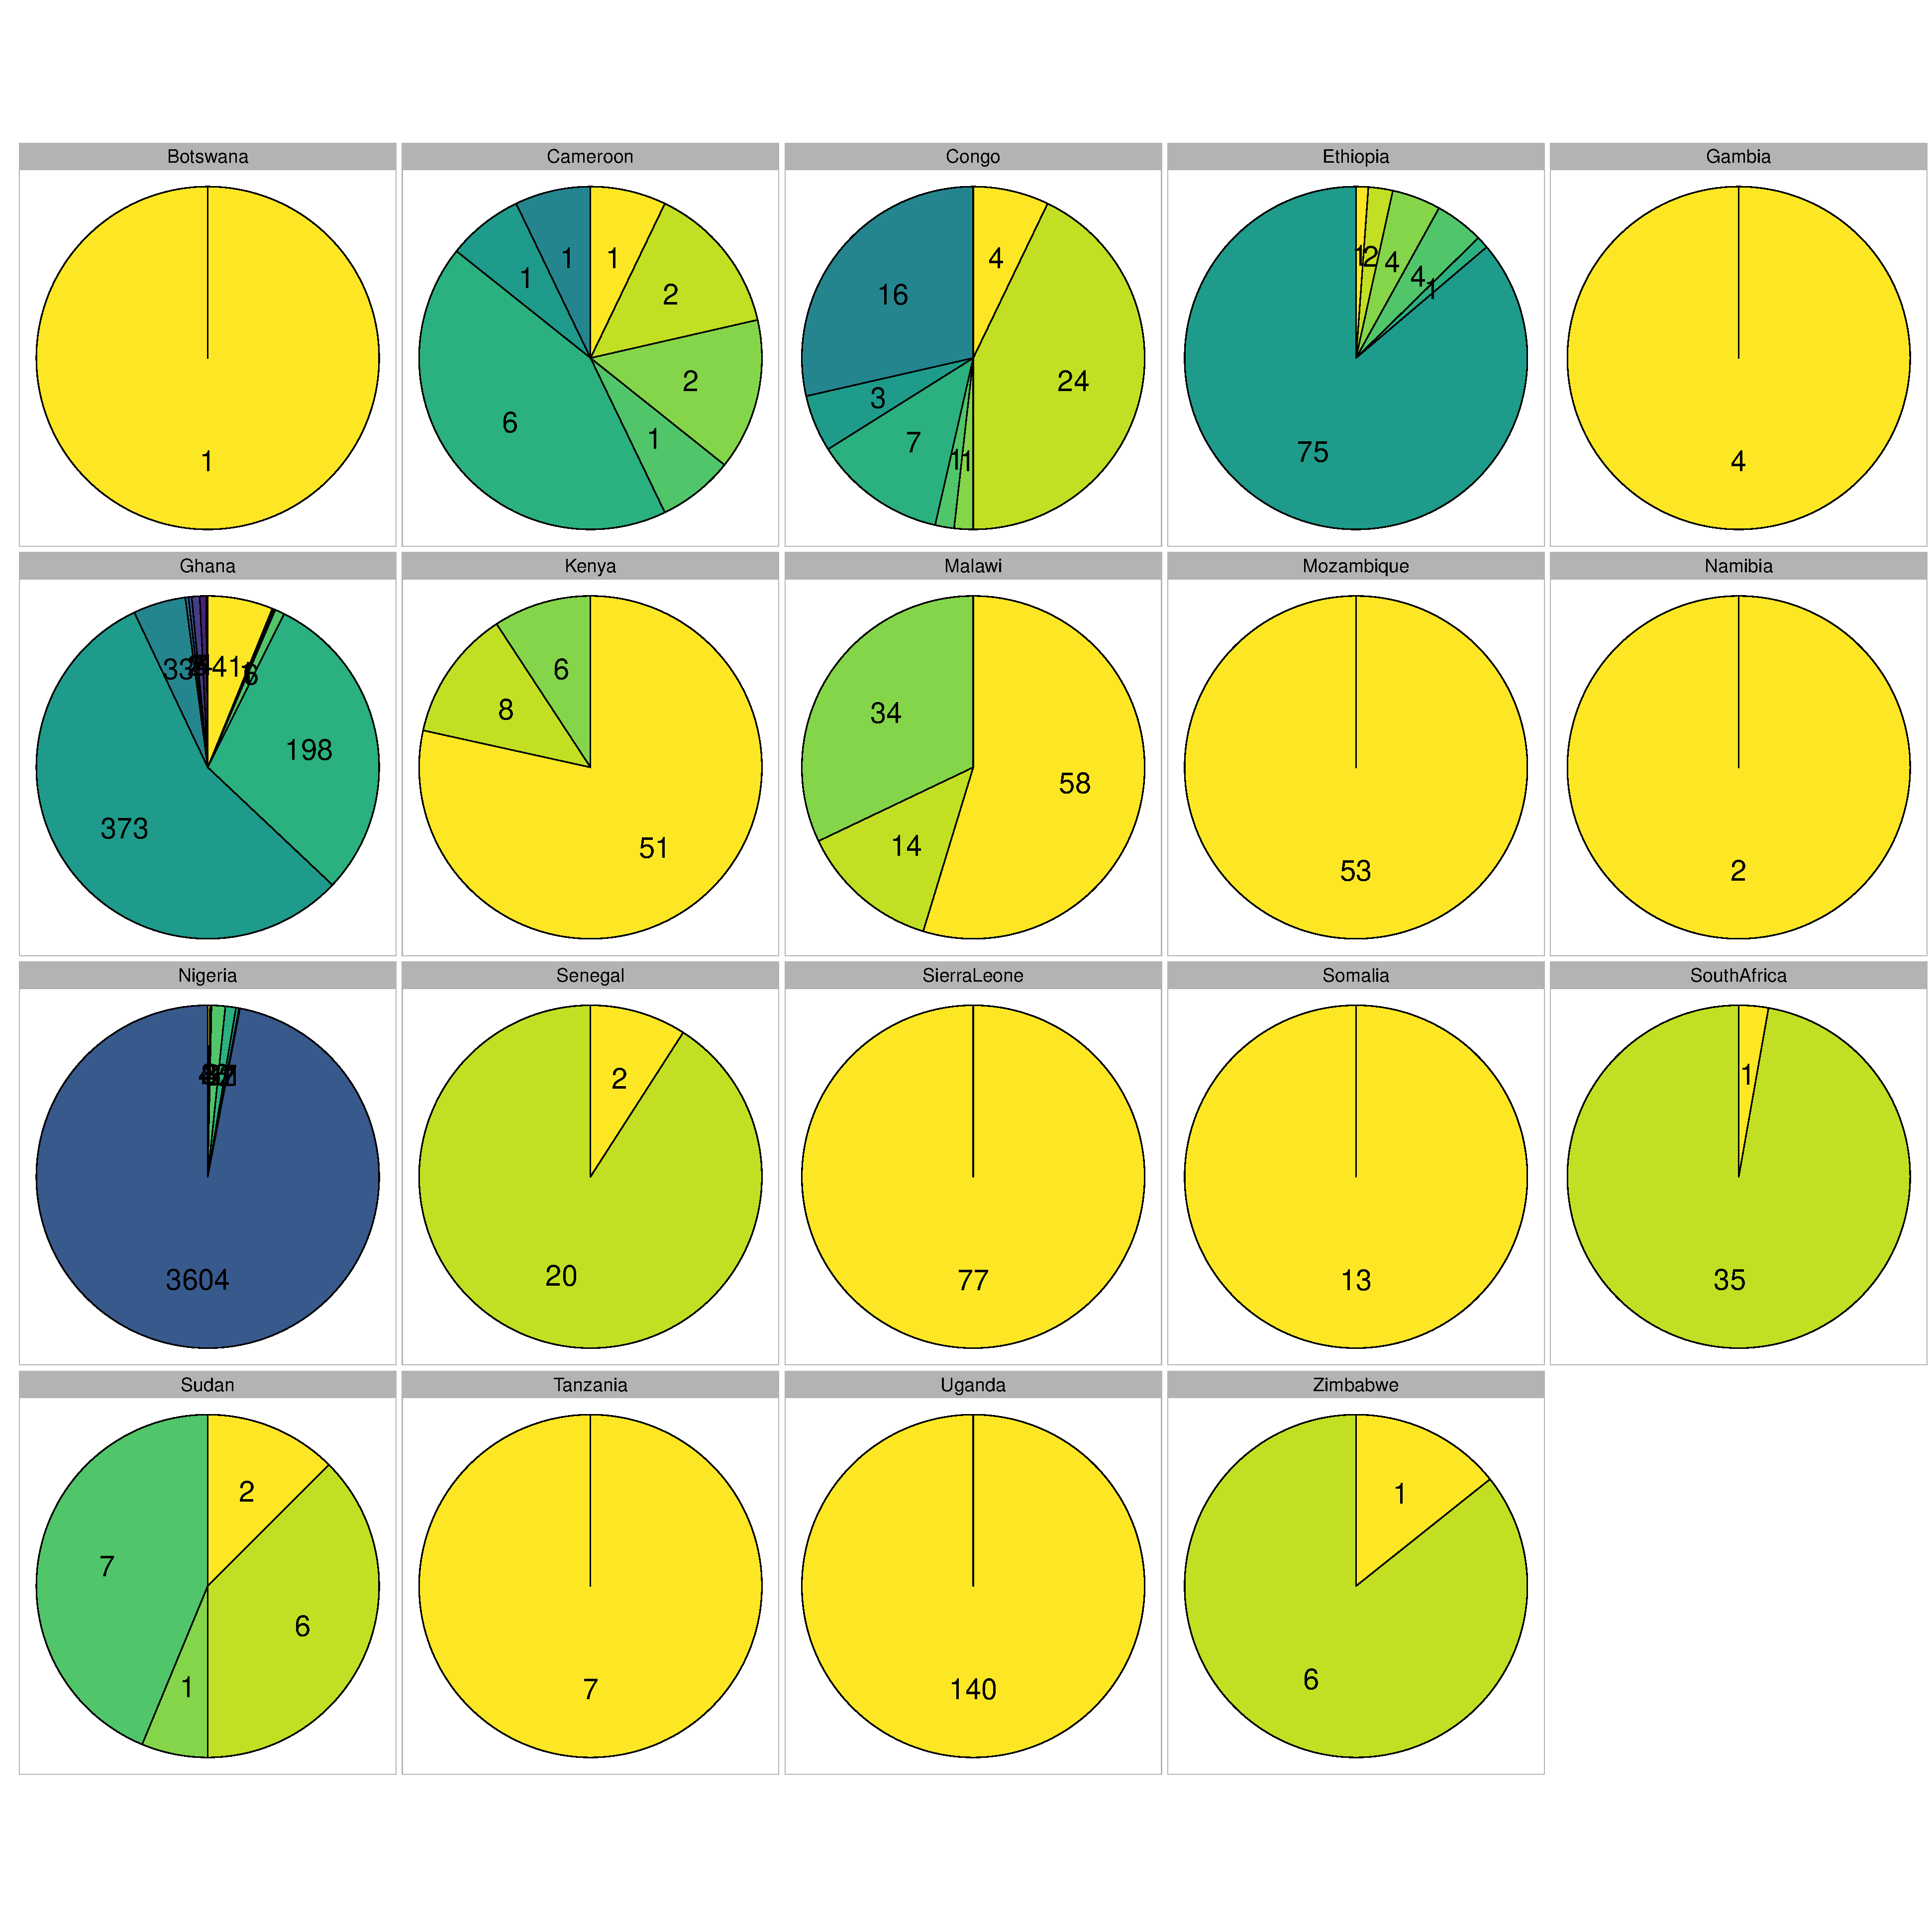
\includegraphics[width=1.0\textwidth]{../images/chapter3/all_countries_SF_props_pie_chart.pdf}
    \caption{Variation of individuals assigned to different ethnic groups by country of assigned group. Each panel represents all individuals assigned to an ethnic group from that country, with proportions of each pie corresponding to proportion of individuals of that ethnic group in that country. Numbers within each slice correspond to total number of individuals within a given ethnic group.}
    \label{fig:all_countries_SF_props_pie_chart}
\end{figure}

Some other patterns can be noted. Whilst many individuals have intermediate levels of ancestry from West African populations (e.g. Ghana\_Fante or Yoruba\_Yoruba), much fewer individuals have intermediate levels of Ethiopia\_Somali ancestry (Fig. \ref{fig:SF_props_distribution_top30}). This may be because Somalis are more recent immigrants to the UK and therefore tend to be less admixed with Europeans relative to other immigrant populations which have been in the U.K. longer and hence can be modelled as a mixture of almost entirely Ethiopia\_Somali ancestry. 

To test whether this was the case, I selected individuals assigned to either Ethiopia\_Somali, Yoruba or Ghana\_Fante and estimated their proportions of total African, European and Asian ancestry using SOURCEFIND. Individuals from Yoruba and Ghana\_Fante had, on average, 6.2\% and 5.2\% European ancestry respectively, whereas individuals from Ethiopia\_Somali had 0.21\% on average, suggesting they are indeed less mixed than other populations, which is consistent with them being more recent migrants. 

\subsection{Verifying painting accuracy} 
 
Not all individuals within the U.K. Biobank were born in the U.K.; visualising the ancestry distribution of these individuals allows ensures us that the painting is accurate and may reveal insights into population history. For instance, the ancestry distribution of individuals born in the Caribbean may provide evidence for where in Africa slaves forcibly transported to the Caribbean during the transatlantic slave trade originated from. This is important, as disembarkation records from the Slave Trade are often sparse, meaning many people with African ancestry who currently live in the Americas may not have knowledge of where their ancestors originated from.

I subsetted the coancestry matrix to contain only U.K. Biobank individuals who provided data on birth location (n=6153/8472). We would expect that individuals who were born in a particular country would copy the most from reference populations from that country. For example, we would expect individuals who were born in South Africa to copy the most from sampled Bantu and Zulu ethnic groups from South Africa. This may not always be the case, as some ethnic groups have crossed borders in their history,  or we may not have sampled representative groups from some countries, but it may broadly be expected to be true. We also have birth place data for individuals who were not born in Africa (e.g. the Caribbean and Brazil). 

\begin{figure}[htp]
    \centering
    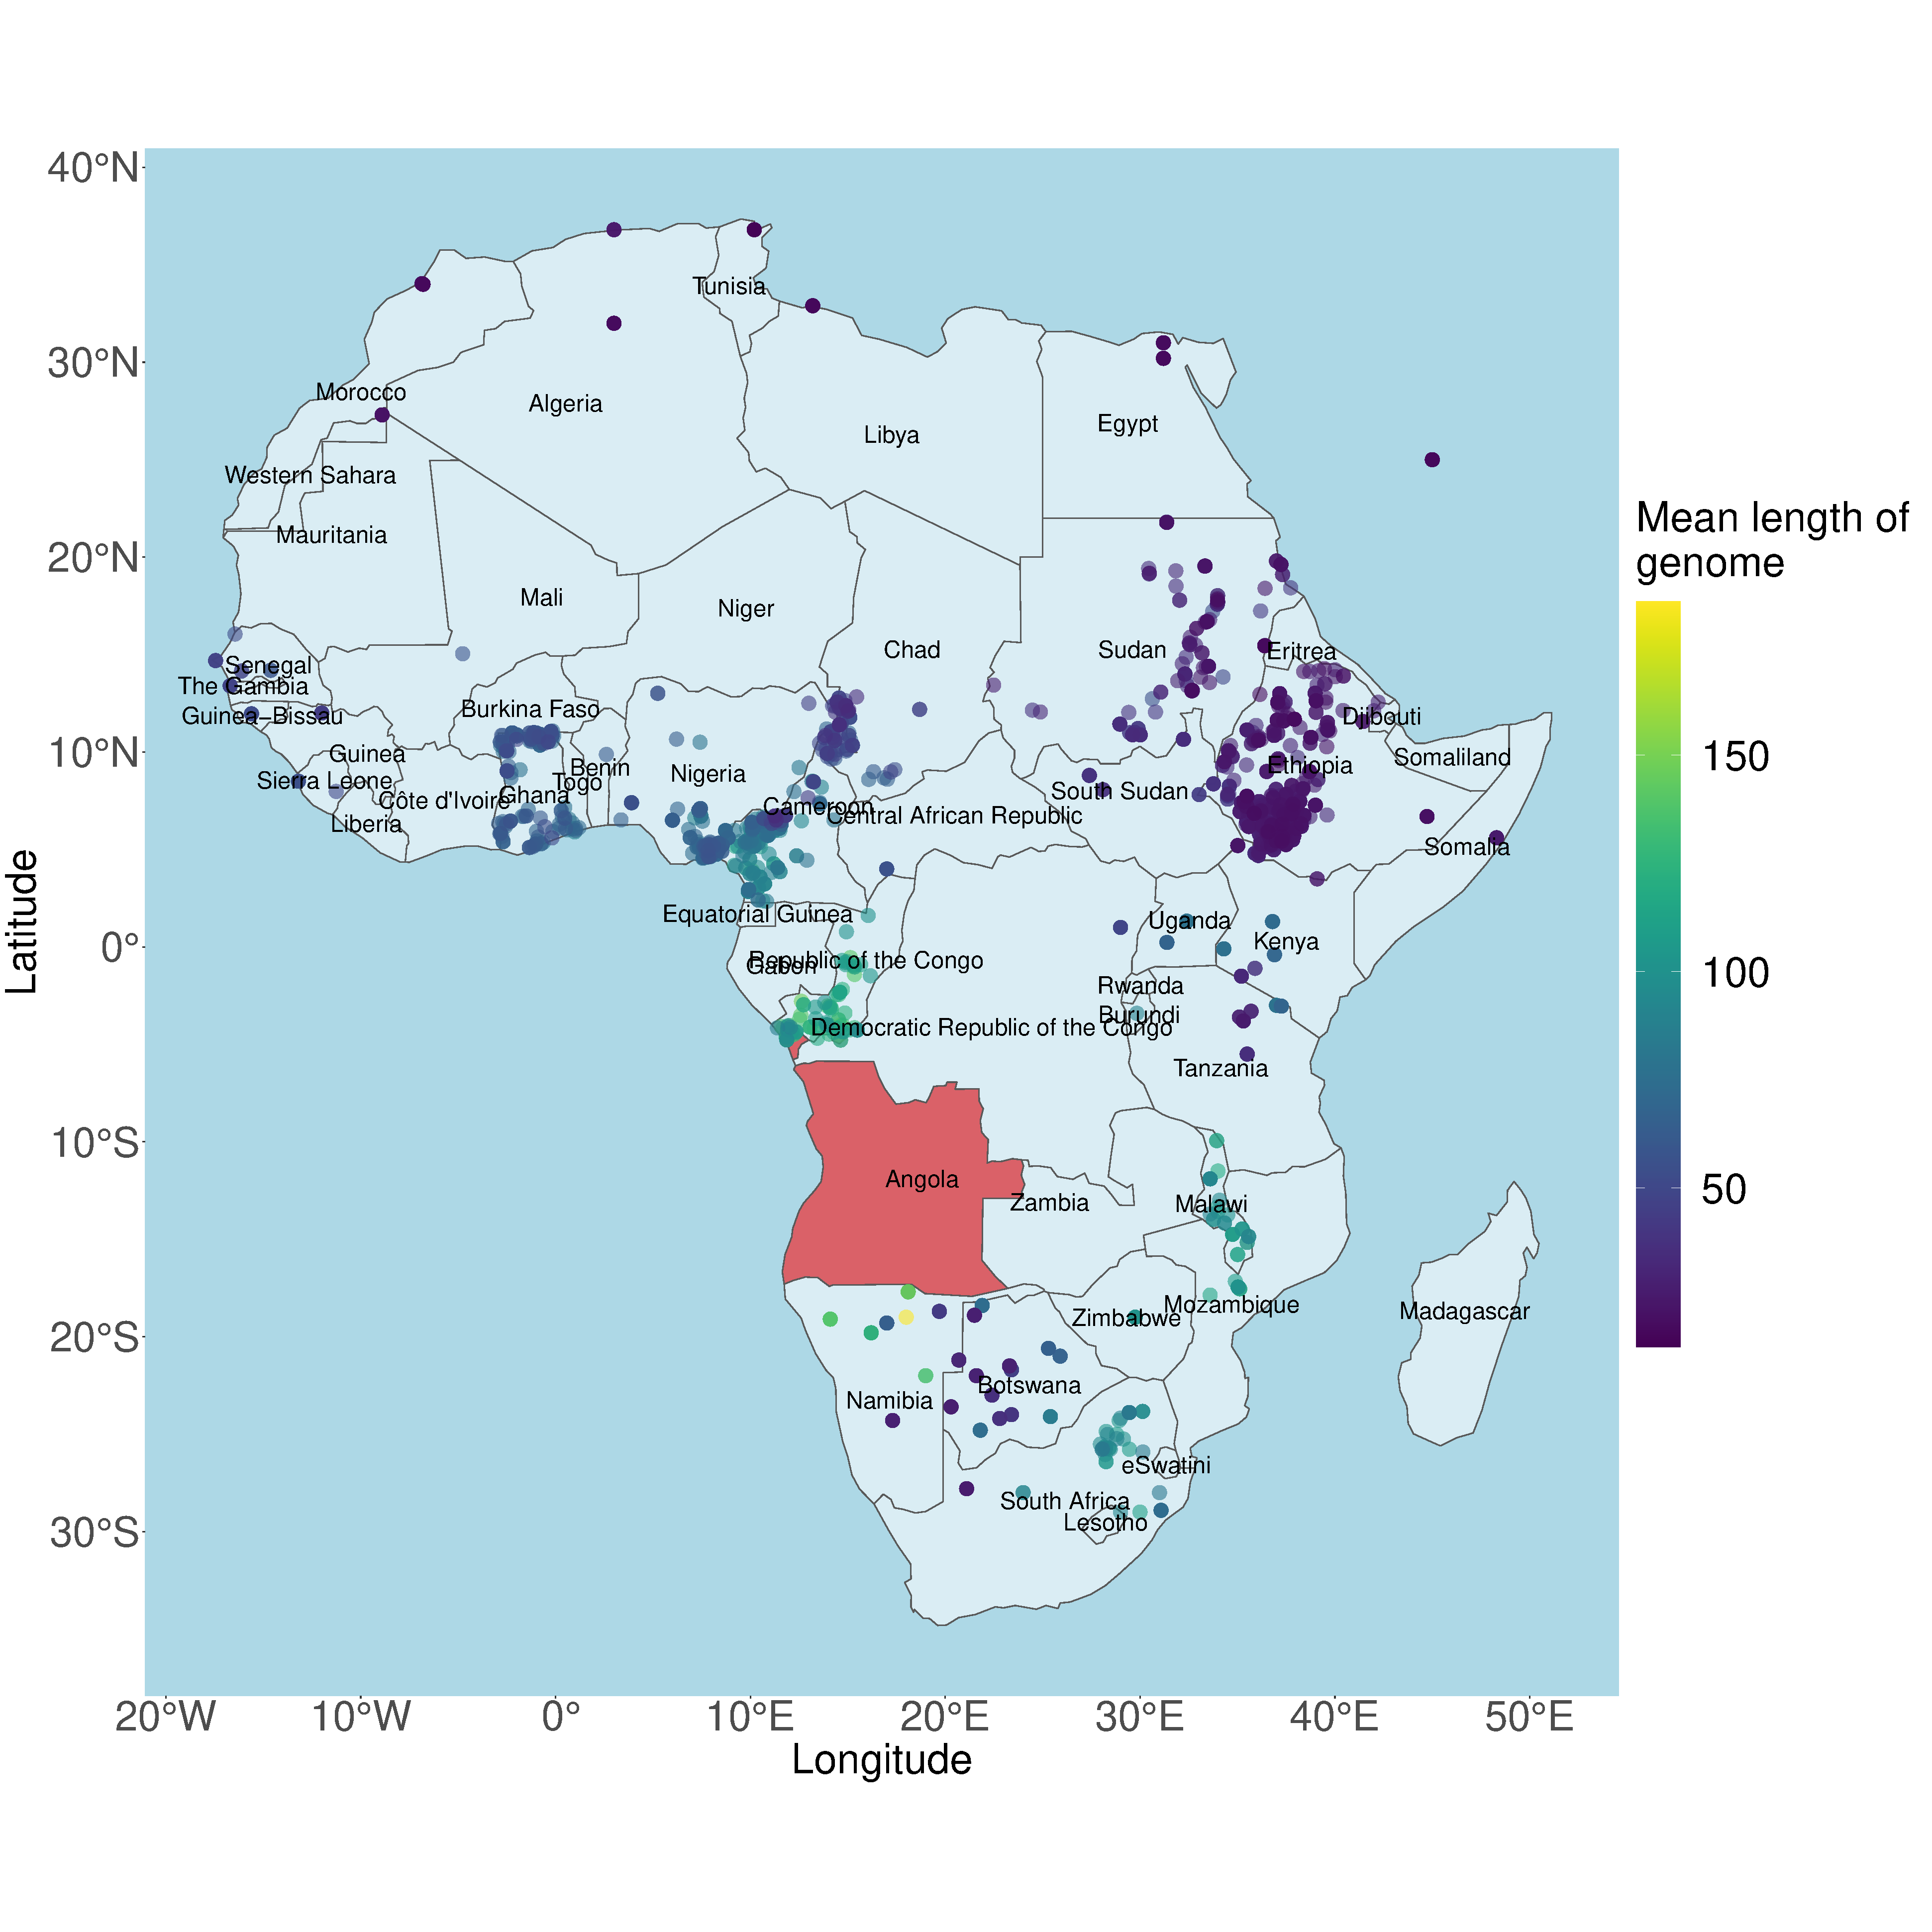
\includegraphics[width=1.0\textwidth]{../images/chapter3/haplotype_map_SouthAfrica.pdf}
    \caption{Map of haplotype donation to U.K. Biobank individuals born in South Africa. Each point represents one Human Origins population, coloured according to the summed amount of chunklengths that population donates to all U.K. Biobank individuals born in South Africa. }
    \label{fig:haplotype_map_SouthAfrica}
\end{figure}

Fig. \ref{fig:haplotype_map_SouthAfrica} shows the map of haplotype donation from reference groups to U.K. Biobank individuals born in South Africa. It is clear that reference populations from South Africa, in particular the Zulu ethnic group, contribute the most to these individuals. The pattern is qualitatively the same for all countries which had a reasonable number of donor populations, suggesting that the painting had good resolution down to at least the level of individual countries (Fig \ref{fig:country_of_origin_allInds}).

There are several interesting results. For example, there are 2,263 individuals who were born in the Caribbean. Visualising the haplotype donation map for these individuals shows that they are primarily of West African ancestry (supplementary figure \ref{fig:haplotype_map_Caribbean}), consistent with historical evidence \cite{micheletti2020genetic}. Individuals born in Brazil have ancestry from further South, again consistent with historical evidence (supplementary figure \ref{fig:haplotype_map_Brazil}). Of the nine individuals born in Brazil, six of them had a majority SOURCEFIND component from an ethnic group in The Republic of the Congo. However, it should be noted that there is a relatively small sample size from individuals born in Brazil (n=9), and that these individuals may not be representative of the Brazilian population as a whole. 

As a formal test of the painting accuracy, I estimated SOURCEFIND ancestry proportions in each retained U.K. Biobank individual. An individual was `assigned' to a particular ethnic group if they had 75\% or more of their total ancestry from that group. If the country the assigned reference population is from matches the birth location of the individual, then I considered that a `success' and a `fail' otherwise. Individuals who were born in the U.K. or who had no birth country were excluded from this analysis. 75\% was chosen as an arbitrary threshold. 

\begin{figure}[htp]
    \centering
    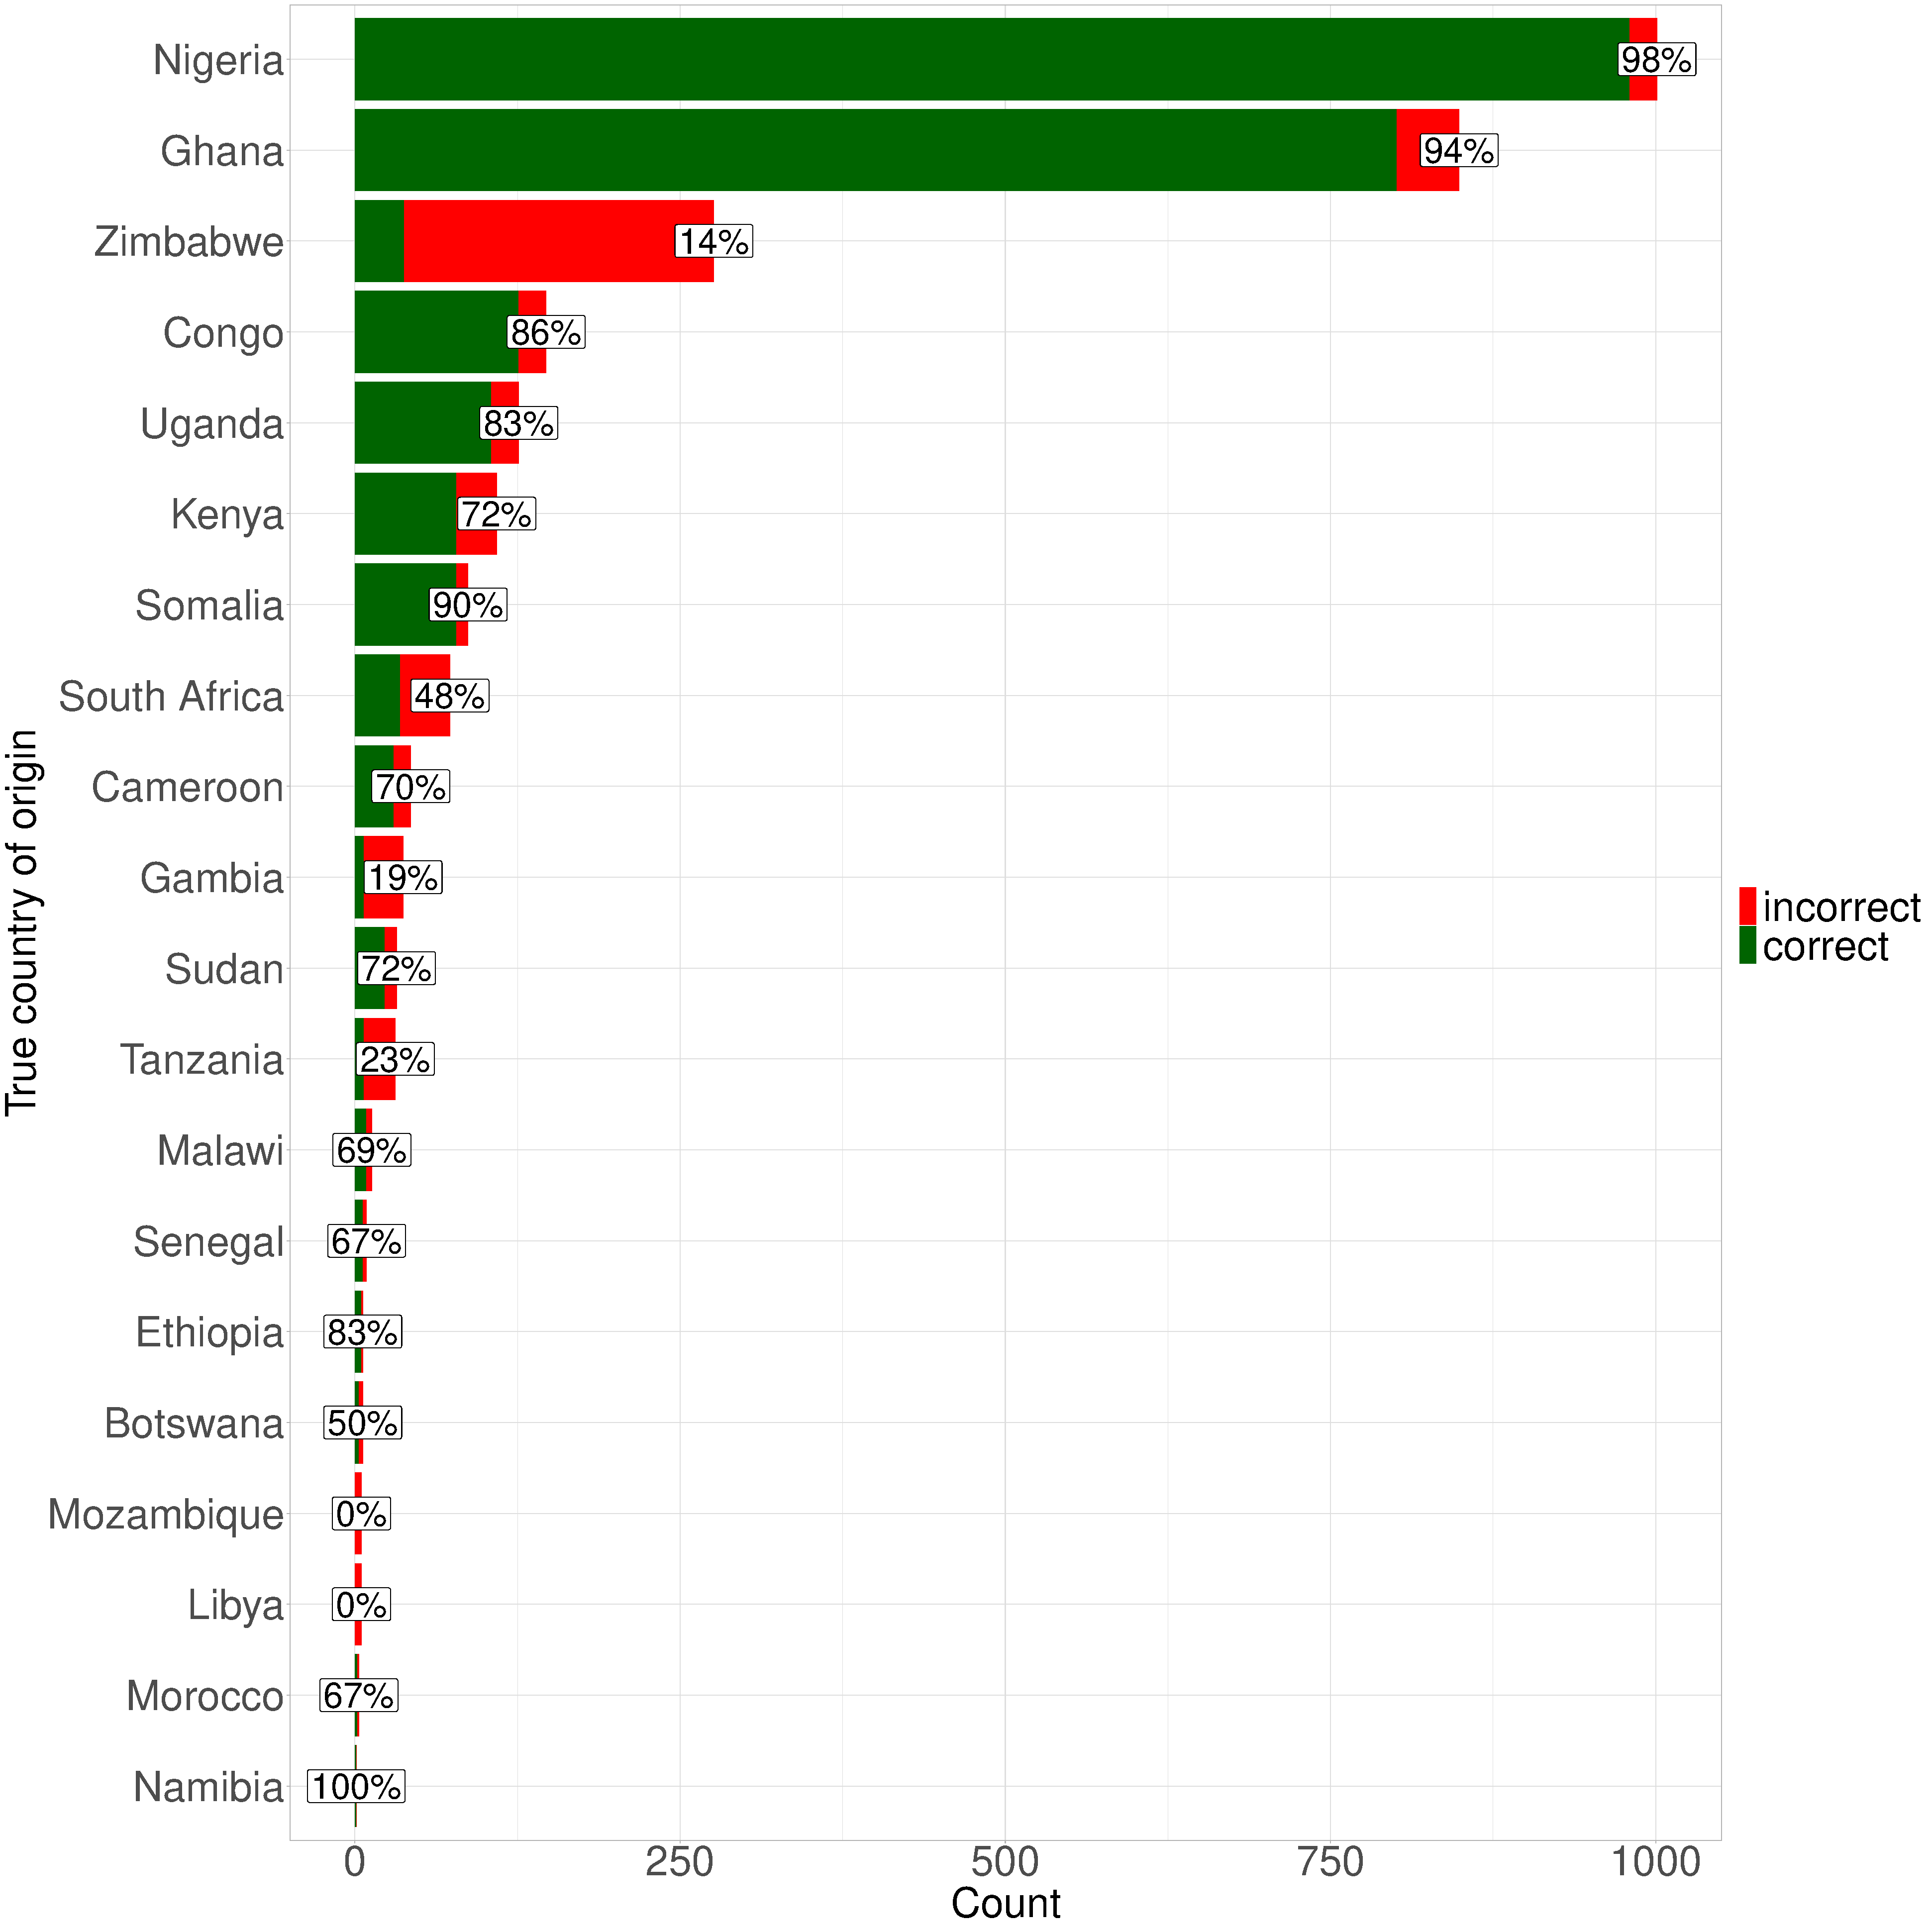
\includegraphics[width=1.0\textwidth]{../images/chapter3/country_of_origin_allInds.pdf}
    \caption{Correspondence of true birth country with estimated birth country. Each bar corresponds to a true birth country, with the length of the bar corresponding to the total number of people in our dataset born in that country. The green section corresponds to the total number of individuals where the birth country was correctly guessed and the red section to those who were incorrectly guessed. Percentage labels give percentage correct for that country.}
    \label{fig:country_of_origin_allInds}
\end{figure}

The overall accuracy at predicting birth location across all individuals was 81.63\%, suggesting there was substantial information within the coancestry matrix. For certain countries where there was large number of surrogate populations, such as Ghana and Nigeria, the prediction accuracy was high. For other countries, the prediction accuracy was much lower. For example, Tanzania, which is only represented by a single reference population, had a prediction accuracy of 23\%. Zimbabwe had by far the lowest prediction accuracy (14\%) out of countries with more than 100 U.K. Biobank individuals. Of the 266 individuals born in Zimbabwe, 194 were assigned to an ethnic group from outside Zimbabwe; 74 to Malawi\_Chewa, 71 to Mozambique\_Mozambique and 49 to Malawi\_Yao. Individuals from the ethnic groups from Malawi are found across Malawi, Zimbabwe and other countries, showing the possible weakness of this approach which aims to categorise individuals into a single country, as ethnic groups often transcend countries. Indeed we only have data from one (partially) Zimbabwean group, the Zulu, who may not well-reflect the ancestors of U.K. Biobank participants born in Zimbabwe.

I performed the same analysis but using the data which had been imputed. This stands as a practical test of whether it is preferable to impute or retain a smaller number of non-imputed SNPs when estimating country-level haplotype variation. This yielded an accuracy of 81.89\%, a value almost identical to that obtained with the dataset containing approximately 70,000 non-imputed SNPs, despite my earlier results indicating that sub-country population assignment results are less accurate if using imputed data due to reference bias (Table \ref{table:TVD_copying}). This may be because this broad-scale assignment of individuals to countries is not as affected by imputation as a more subtle dissection of sub-country ancestry. To test whether this is the case, I took all ethnic groups from Nigeria, Cameroon and Ghana in the Human Origins dataset which had five or more individuals (n=51 populations, n=1203 individuals), and for each individual, estimated ancestry proportions of each of the 51 populations. I performed this analysis for both datasets containing no imputed SNPs and 70\% imputed SNPs. For each dataset, I took the average proportion of ancestry for each ethnic group across all individuals. 

Fig \ref{fig:SOURCEFIND_imp_nonimp} shows that there are substantial differences between the proportions obtained from imputed and non-imputed datasets, showing sub-country assignment is affected by imputation. In particular, there is less variance across the proportions for the imputed dataset (var=0.67) relative to the non-imputed dataset (var=0.87). This is clear on the figure, as there are many population bunched around the 2\% point for the imputed dataset; the same populations are spread across a wider range of values for the non-imputed dataset. 

\begin{figure}[htp]
    \centering
    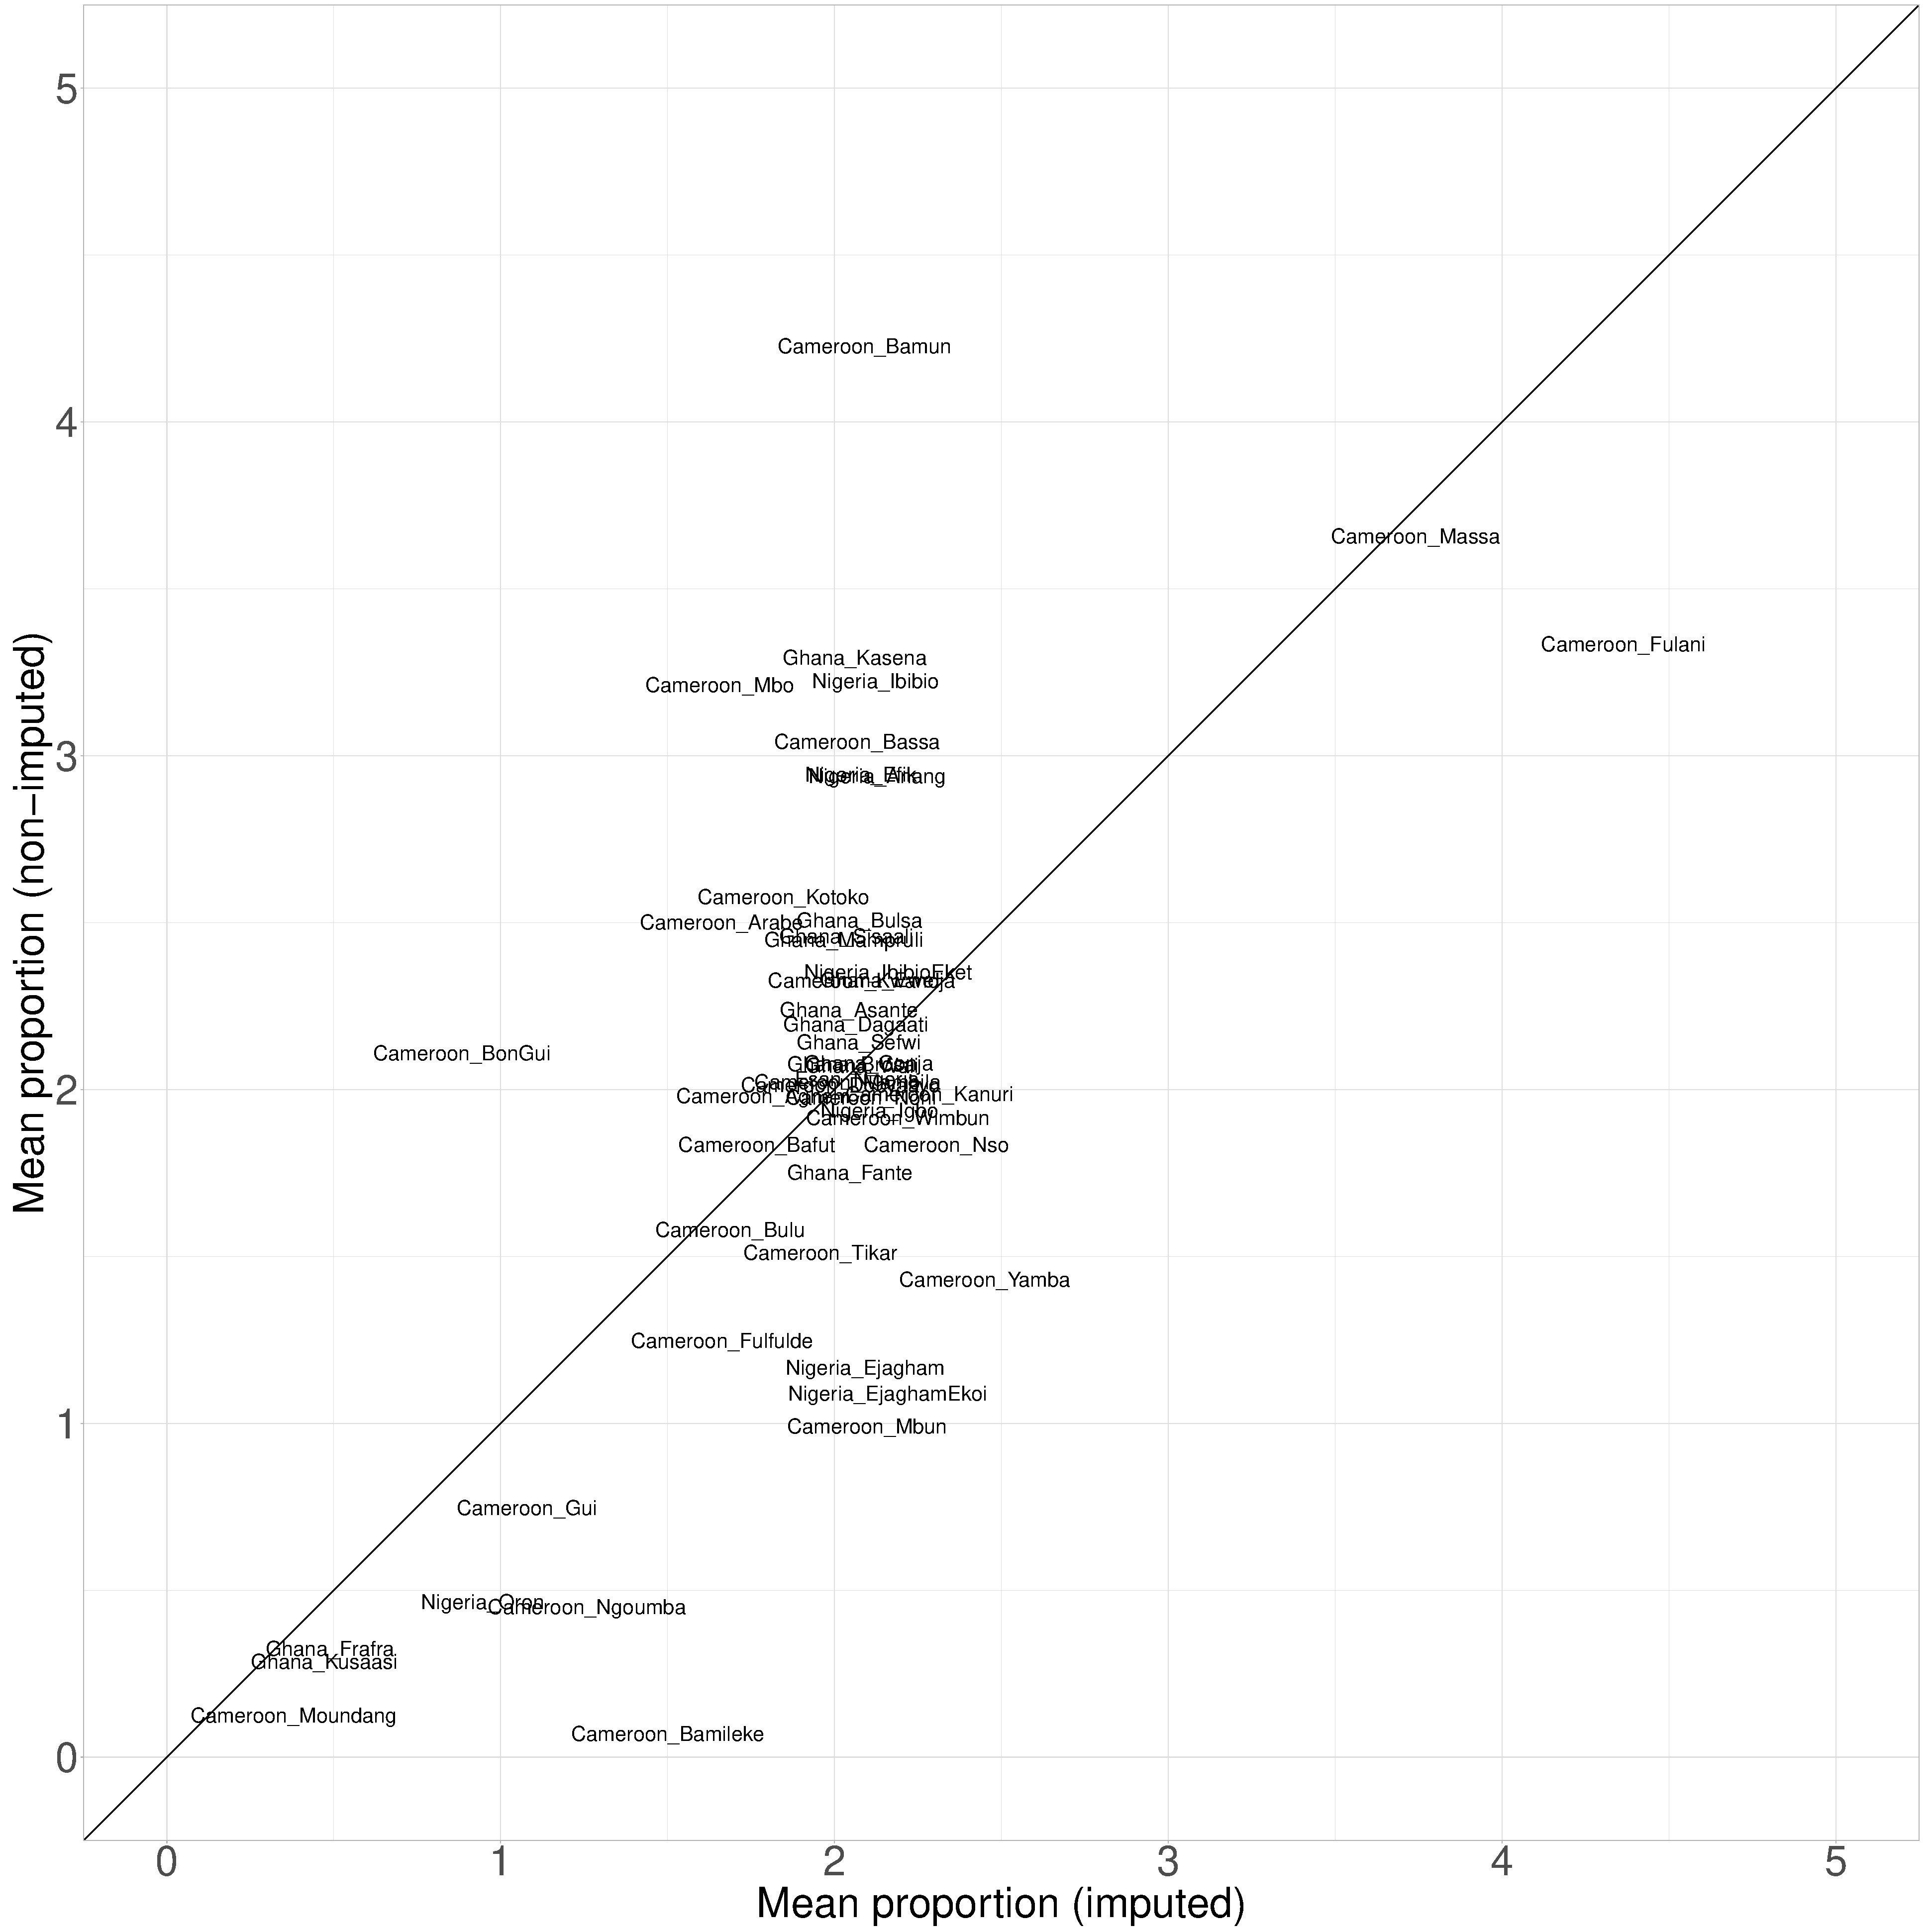
\includegraphics[width=1.0\textwidth]{../images/chapter3/SOURCEFIND_imp_nonimp.pdf}
    \caption{Mean ancestry proportions averaged across 1203 individuals from Ghana, Nigeria and Cameroon of 51 populations from the same countries. Proportions obtained from data containing 70\% imputed SNPs (x-axis) and no imputed SNPs (y-axis).}
    \label{fig:SOURCEFIND_imp_nonimp}
\end{figure}


\subsection{Patterns of African ancestry across the U.K.}

The U.K. Biobank dataset contains data on the testing centre that each individual registered at. I used this information to determine whether there was structure in how individuals with recent African ancestry are distributed across the U.K. There were no apparent outliers in terms of any centres with substantially larger proportion of individuals who had at least 50\% African ancestry than others (Supplementary Fig. \ref{fig:testing_centre_afr_prop}). However, as expected, centres in large cities such as Barts, Croydon and Hounslow (London), Birmingham and Manchester had the highest proportion of individuals with at least 50\% African ancestry.

I then plotted the distribution of people with recent ancestry related to African ethnic groups at different centres on a map of the U.K (Fig. \ref{fig:SF_props_pie_chart_entropy_map}). No clear pattern was apparent, other than Yoruban ancestry dominating most centres, with some smaller testing centres only containing individuals inferred as having Yoruba-related ancestry.  
 
I estimated the information entropy, $E$, of each assessment centre based on the SOURCEFIND proportions, similar to previous work performed by van Dorp et al (2018), who used the principle of entropy to determine the extent to which individuals from different ethnic groups were scattered across different clusters \cite{van2019genetic}.

To evaluate the extent to which individuals assigned to each ethnic group registered at different testing centers, I calculated entropy given by Schutze et al (2008) as $\sum_{i=1}^{L} [p_{i,j} \cdot log(p_{i,j})]$ \cite{schutze2008introduction}, where $p_{i,j} = \frac{m_{i,j}}{m_{j}}$, $m_{j}$ is the number of individuals from testing center $j$ assigned to ethnic group $i$ and $m_{ij}$ is the number of ethnic groups to which individuals from center $j$ are assigned. Testing centres in large cities such as London and Birmingham had the highest information entropy, consistent with prior expectations that large cities would contain a higher diversity of ancestries (Fig. \ref{fig:SF_props_pie_chart_entropy_map}). 


\begin{sidewaysfigure}
    \centering
    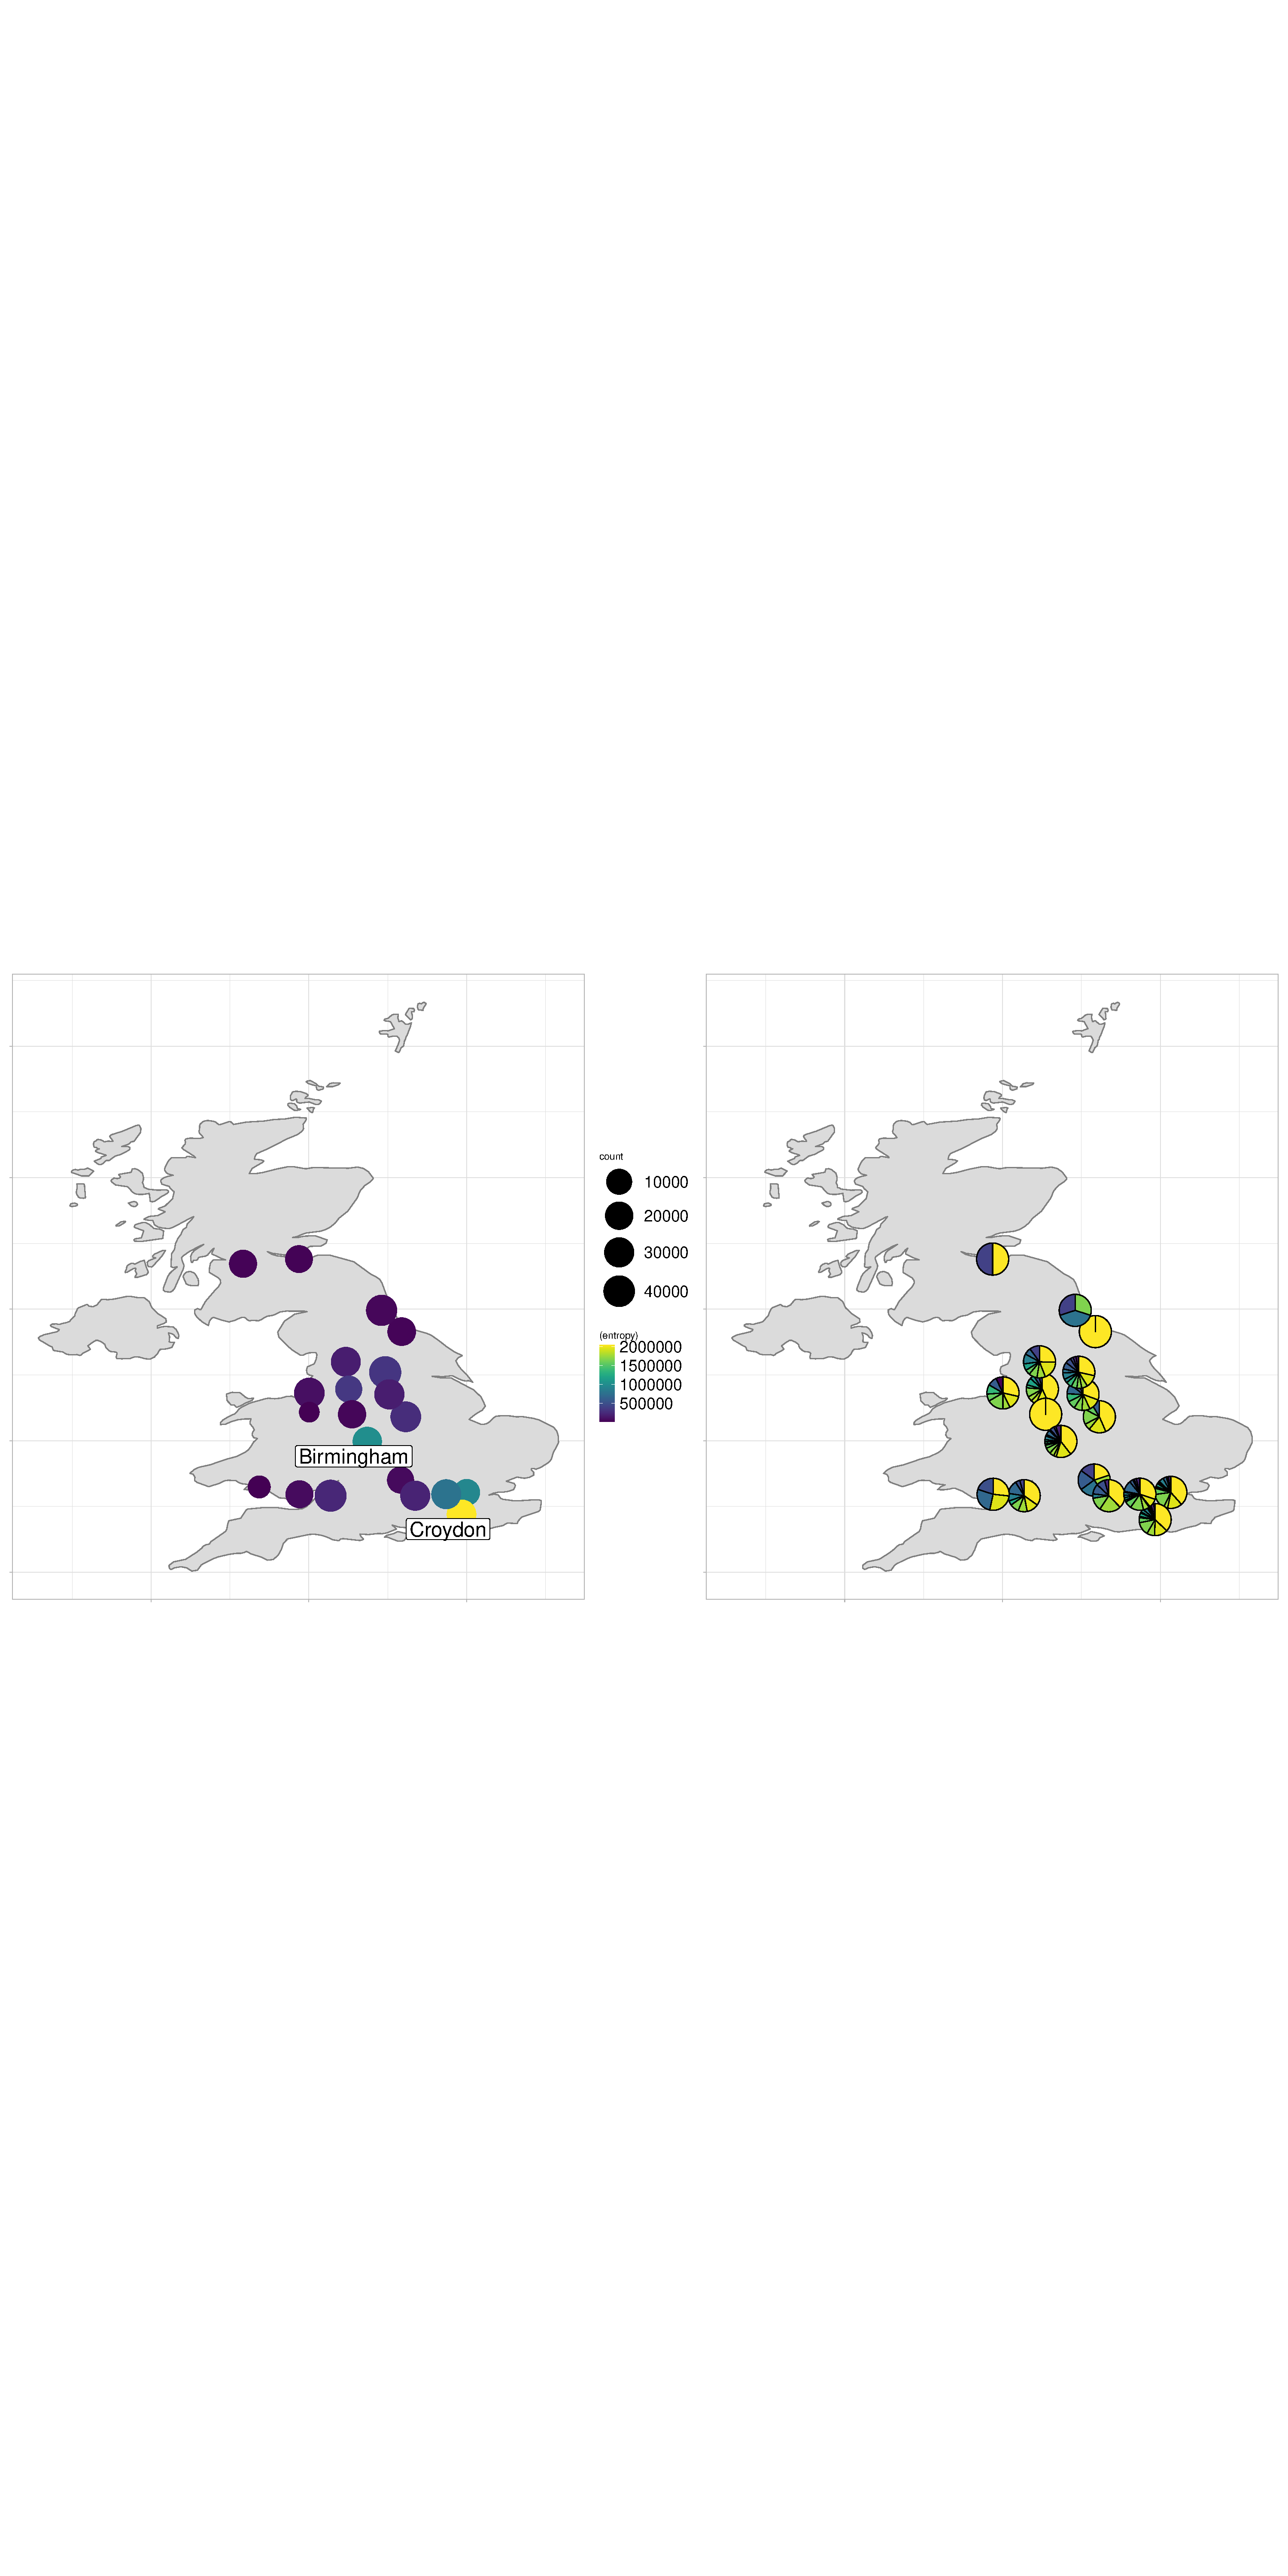
\includegraphics[width=1.0\textwidth]{../images/chapter3/SF_props_pie_chart.pdf}
    \vspace{-1mm}
    \caption{Distribution of ethnicities across different testing centres. Each pie corresponds to a U.K. Biobank testing centre, with each section of the each pie corresponding to a different ethnicity. Jitter added to points to avoid overlapping. }
    \label{fig:SF_props_pie_chart_entropy_map}
\end{sidewaysfigure}

\subsection{Patterns of African ancestry across the U.K.}

I also had access to the birth-date of each U.K. Biobank participant. Therefore, it is possible to calculate the increase of the ancestry of a particular ethnic group over time based on birth-year (Fig.  \ref{fig:rollingaverage_time_Buganda_ancestry}). I took all U.K. Biobank individuals with more than 50\% African ancestry and split them into 50 bins according to their birth date. Using a rolling window in the \texttt{rollyapply} function from the \texttt{zoo} R library, I calculated the mean proportion of all ancestries across ancestry for each bin. Fig \ref{fig:rollingaverage_time_Buganda_ancestry} shows the increase of Buganda ancestry over time. 

\begin{figure}[htp]
    \centering
    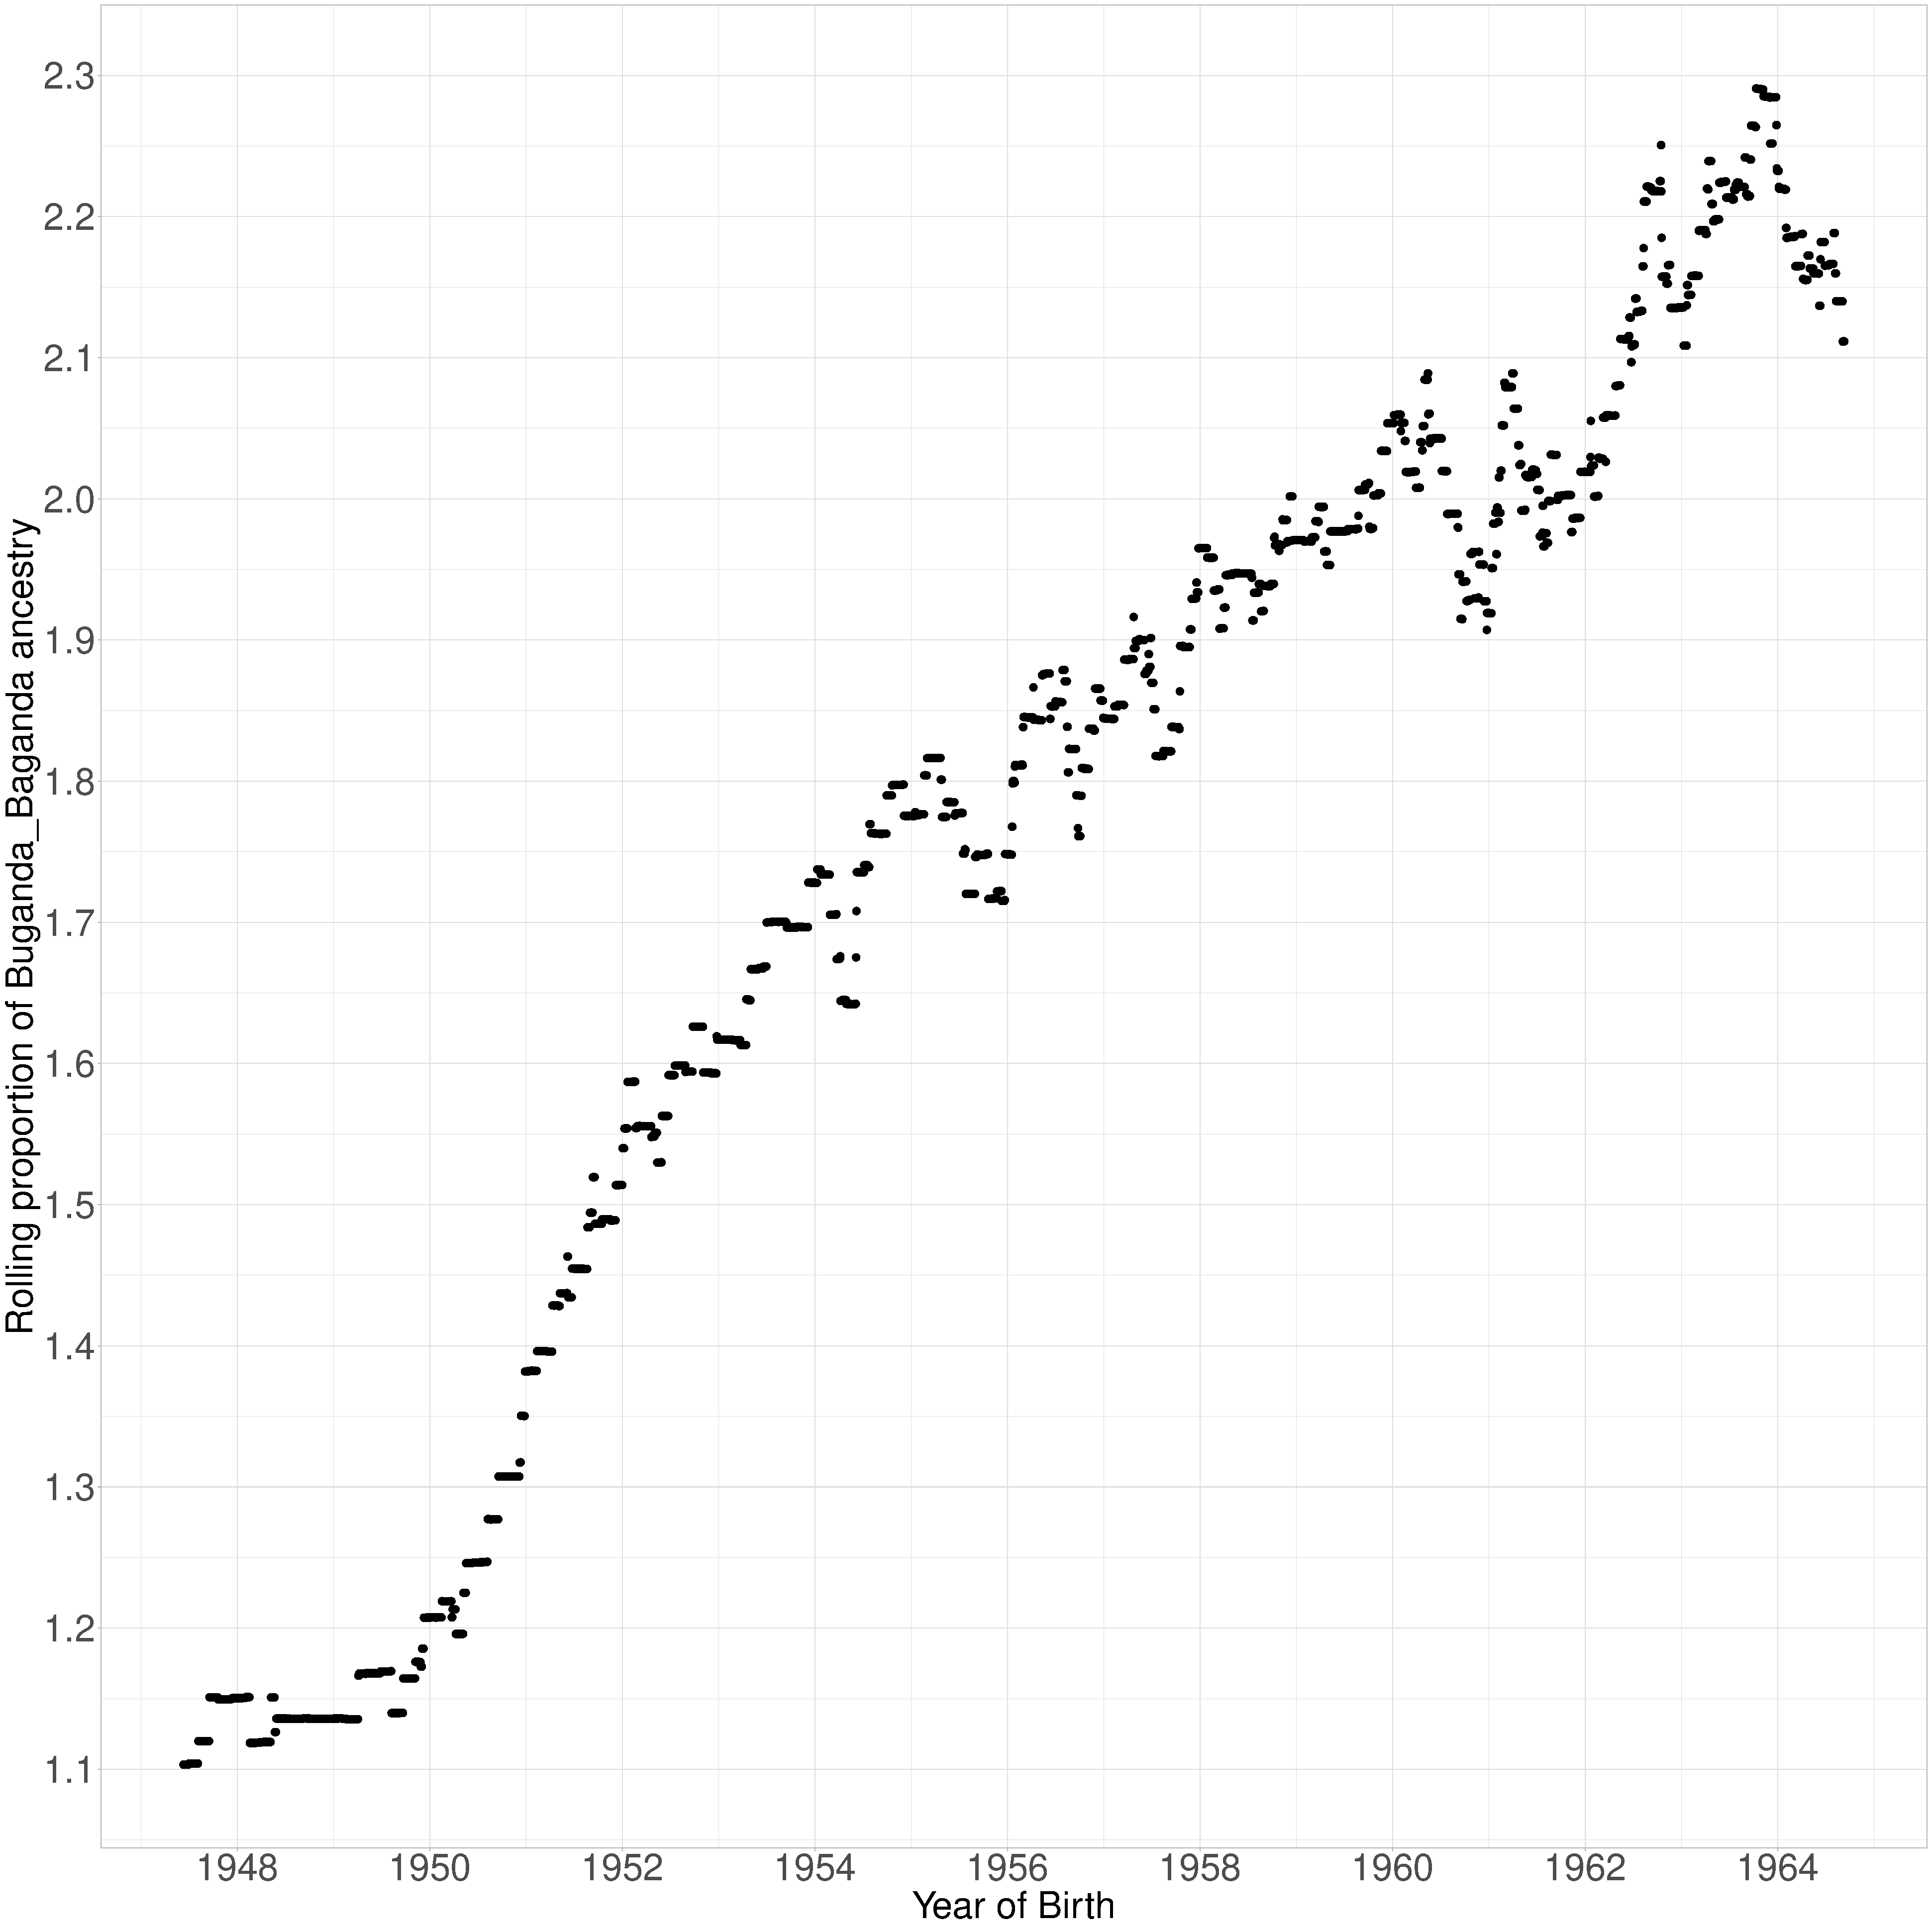
\includegraphics[width=1.0\textwidth]{../images/chapter3/rollingaverage_time_Buganda_ancestry.pdf}
    \caption{Increase in the mean proportion of Buganda ancestry between 1948 and 1965. An overlapping sliding window was applied to SOURCEFIND ancestry proportions and mean proportion of Buganda ancestry for each window plotted against the mean birth-date of individuals in that bin.}
    \label{fig:rollingaverage_time_Buganda_ancestry}
\end{figure}

We can observe roughly a doubling of the mean proportion of  Buganda\_Baganda ancestry between 1950 and 1964. In 1972, then president Idi Amin expelled roughly 60,000 Ugandans to the U.K. Therefore, this increase may tentatively correspond to an increase in the number of individuals between the ages of 7-22 arriving in the U.K. during these dates. 

\section{Summary of Results and Discussion} 

The aim of this chapter was twofold; firstly, to determine whether using less dense non-imputed or more dense imputed SNPs is preferable when combining genotype data from multiple chips. Secondly, I wanted to explore the diversity of African ancestry in the U.K. Biobank and its relation to population history.  

I also showed that, in individuals with recent African ancestry, there is enough linkage information across 70,000 genome-wide SNPs to recover a substantial amount of useful haplotype information and accurately predict the birth country of a sample. Further, I found that using imputed genotypes may significantly reduce the power of a painting and introduce a degree of bias towards populations present in a reference panel used for imputation. 

West African ancestry was the most common across samples with recent African ancestry, with ancestry from ethnic groups from Nigeria and Ghana being especially prevalent. In particular, individuals had substantially more ancestry from Yoruba than any other ethnicity. I did not find evidence for structure in how African ancestry was distributed across the U.K., based on the testing centre that participants registered at. 

Future work on using Biobanks to explore population structure and history could focus on two points.
Ideally, I would liked to have painted the entire U.K. Biobank dataset using the Human Origins dataset as a reference panel, rather than restricting analysis to individuals with 50\% recent African ancestry. This would have allowed me to analyse a substantially higher amount of African haplotypes across the entire dataset and this give a more complete extent of African ancestry in the U.K. Thus, the development of efficient methods, likely based on the PBWT, which allow for Biobank-scale datasets to be painted by large reference panels would accelerate research into ethnic minority ancestries. 

Secondly, larger reference panels of worldwide populations and more ethnic groups will allow for a more detailed characterisation of genetic variation.  Similarly, including details on ethnic identity in Biobank projects would improve the resolution at which analysis could be carried out.  



\chapter{Bavaria ancient DNA}
\label{chapterlabel4}

\section{Introduction}

Throughout the Pleistocene and Holocene, Germany has been the setting for many population movements and admixture events of modern humans. The Swabian Alps is home to some of the earliest pieces of symbolic art, dated to at least 32kya \cite{conard2009female} and musical instruments dated to 40kya \cite{conard2009new}, both assigned to the Aurignacian tradition. 

Later, the region was also home to one of the first Neolithic traditions in the \textit{Linearbandkeramik} (LBK), a key culture in the Neolithisation of Europe. Early LBK populations across Germany mixed with the preceding Mesolithic hunter gatherer populations \cite{Lipson2017b, mathieson2015genome, Haak2015,gunther2015ancient, Hofmanova2016}. At the end of the Neolithic, a new ancestry was detected \cite{Haak2015, Allentoft2015}  in concert with the arrival of the Corded Ware Complex \cite{furholt2003absolutchronologische}, most closely related to the Yamnaya Pastoralists from the Pontic-Capsian Steppe. Recent studies using ancient DNA have shown that the arrival of Steppe-related ancestry in Europe occurred no earlier than 2700BC \cite{furtwangler2020ancient} and spread widely shortly after.

During the Bronze Age, cultures closely related to Yamnaya, such as Bell Beakers, Corded Ware and Unetice \cite{Haak2015} appeared across Germany at sites such as Kromsdorf \cite{lee2012emerging} and Tollense \cite{jantzen2011bronze, brinker2013human}. It was later dominated by Iron Age cultures such as Hallstatt and La Tène, which have been shown to be partially continuous with the preceding Bell Beaker culture \cite{Brunel12791}. 
 
In the present-day, Germany represents a boundary point between East and West Europe, with a relatively sharp genetic boundary occurring between Germany and Poland to the east, given their close geographic proximity \cite{novembre2008genes, kayser2005significant, veeramah2011genetic}. However, within Germany, SNP-based studies have shown that there is only very weak substructure \cite{steffens2006snp}. Questions remain as to the origin of this East-West structure; is it recent structure, or did it exist during the Middle Ages or earlier? 

Cherry-Tree cave, or \textit{Kirschbaumhöhle}, represents a unique opportunity to study a transect of southern German samples from the Neolithic to the present-day. The cave represents a relatively untouched layer of stratigraphy, with a large series of radiocarbon dates revealing that human and animal inhabitation of the cave stretches back until at least the Michelsberg Culture in the Early Neolithic \cite{botigue2017ancient}. 

Here, I analyse novel data from 11 medium-to-high coverage samples from two sites from Southern Germany and one site from from Southern Austria. In particular, the samples from Kirschbaumhöhle span from the Late Neolithic to the Iron Age, providing an opportunity to study a time transect in a narrow geographic region (Table. \ref{tab:BavariaSampleInfo}). 

A collaborator, Prof. Joachim Burger, Johannes Gutenberg University Mainz, posed the following three questions. 

\begin{enumerate}
\item \textbf{Second Neolithic immigration wave}. One of the samples (Erg1) is thought to have belonged to the first wave of farmers carrying farming technology from the near-east to Europe, and another (DIN2) to the second wave. Do we observe genetic differences between the two waves of samples and do they show evidence of previously reported hunter-gatherer admixture?
\item \textbf{Cherry Tree Cave}. Do we see evidence of genetic continuity from from the Late Neolithic through to the Iron Age in Cherry Tree Cave?
\item \textbf{Germanic / Slavic divide}. Is there a distinction between the Germanic and Slavic samples from the Middle Age samples? How do these populations compare to the preceding samples from the Bronze and Iron ages?
\end{enumerate}

\section{Methods}

\subsection{Data generation}

Eleven whole-genomes of ancient individuals were generated by collaborators at the Johannes Gutenberg, University of Mainz, Germany. The estimated radiocarbon dates range from 5200B to 1060AD (Fig. \ref{fig:chapter4_intro_SamplesDates}). Six of the samples were found in Cherry-Tree Cave in the Bavarian district of Forchheim, four from futher South in the region of Dingolfing/Essenbach and one sample from Molzbichl in southern Austria (Fig. \ref{fig:chapter4_intro_SamplesMap}). The samples had a median coverage of 4.84x and ranged from 0.7x to 17.52x. Full details of coverage, location and dates are given in Table \ref{tab:BavariaSampleInfo}.

I was given the data of each newly sequenced sample in \texttt{vcf} format. 

\begin{figure}[htp]
    \centering
    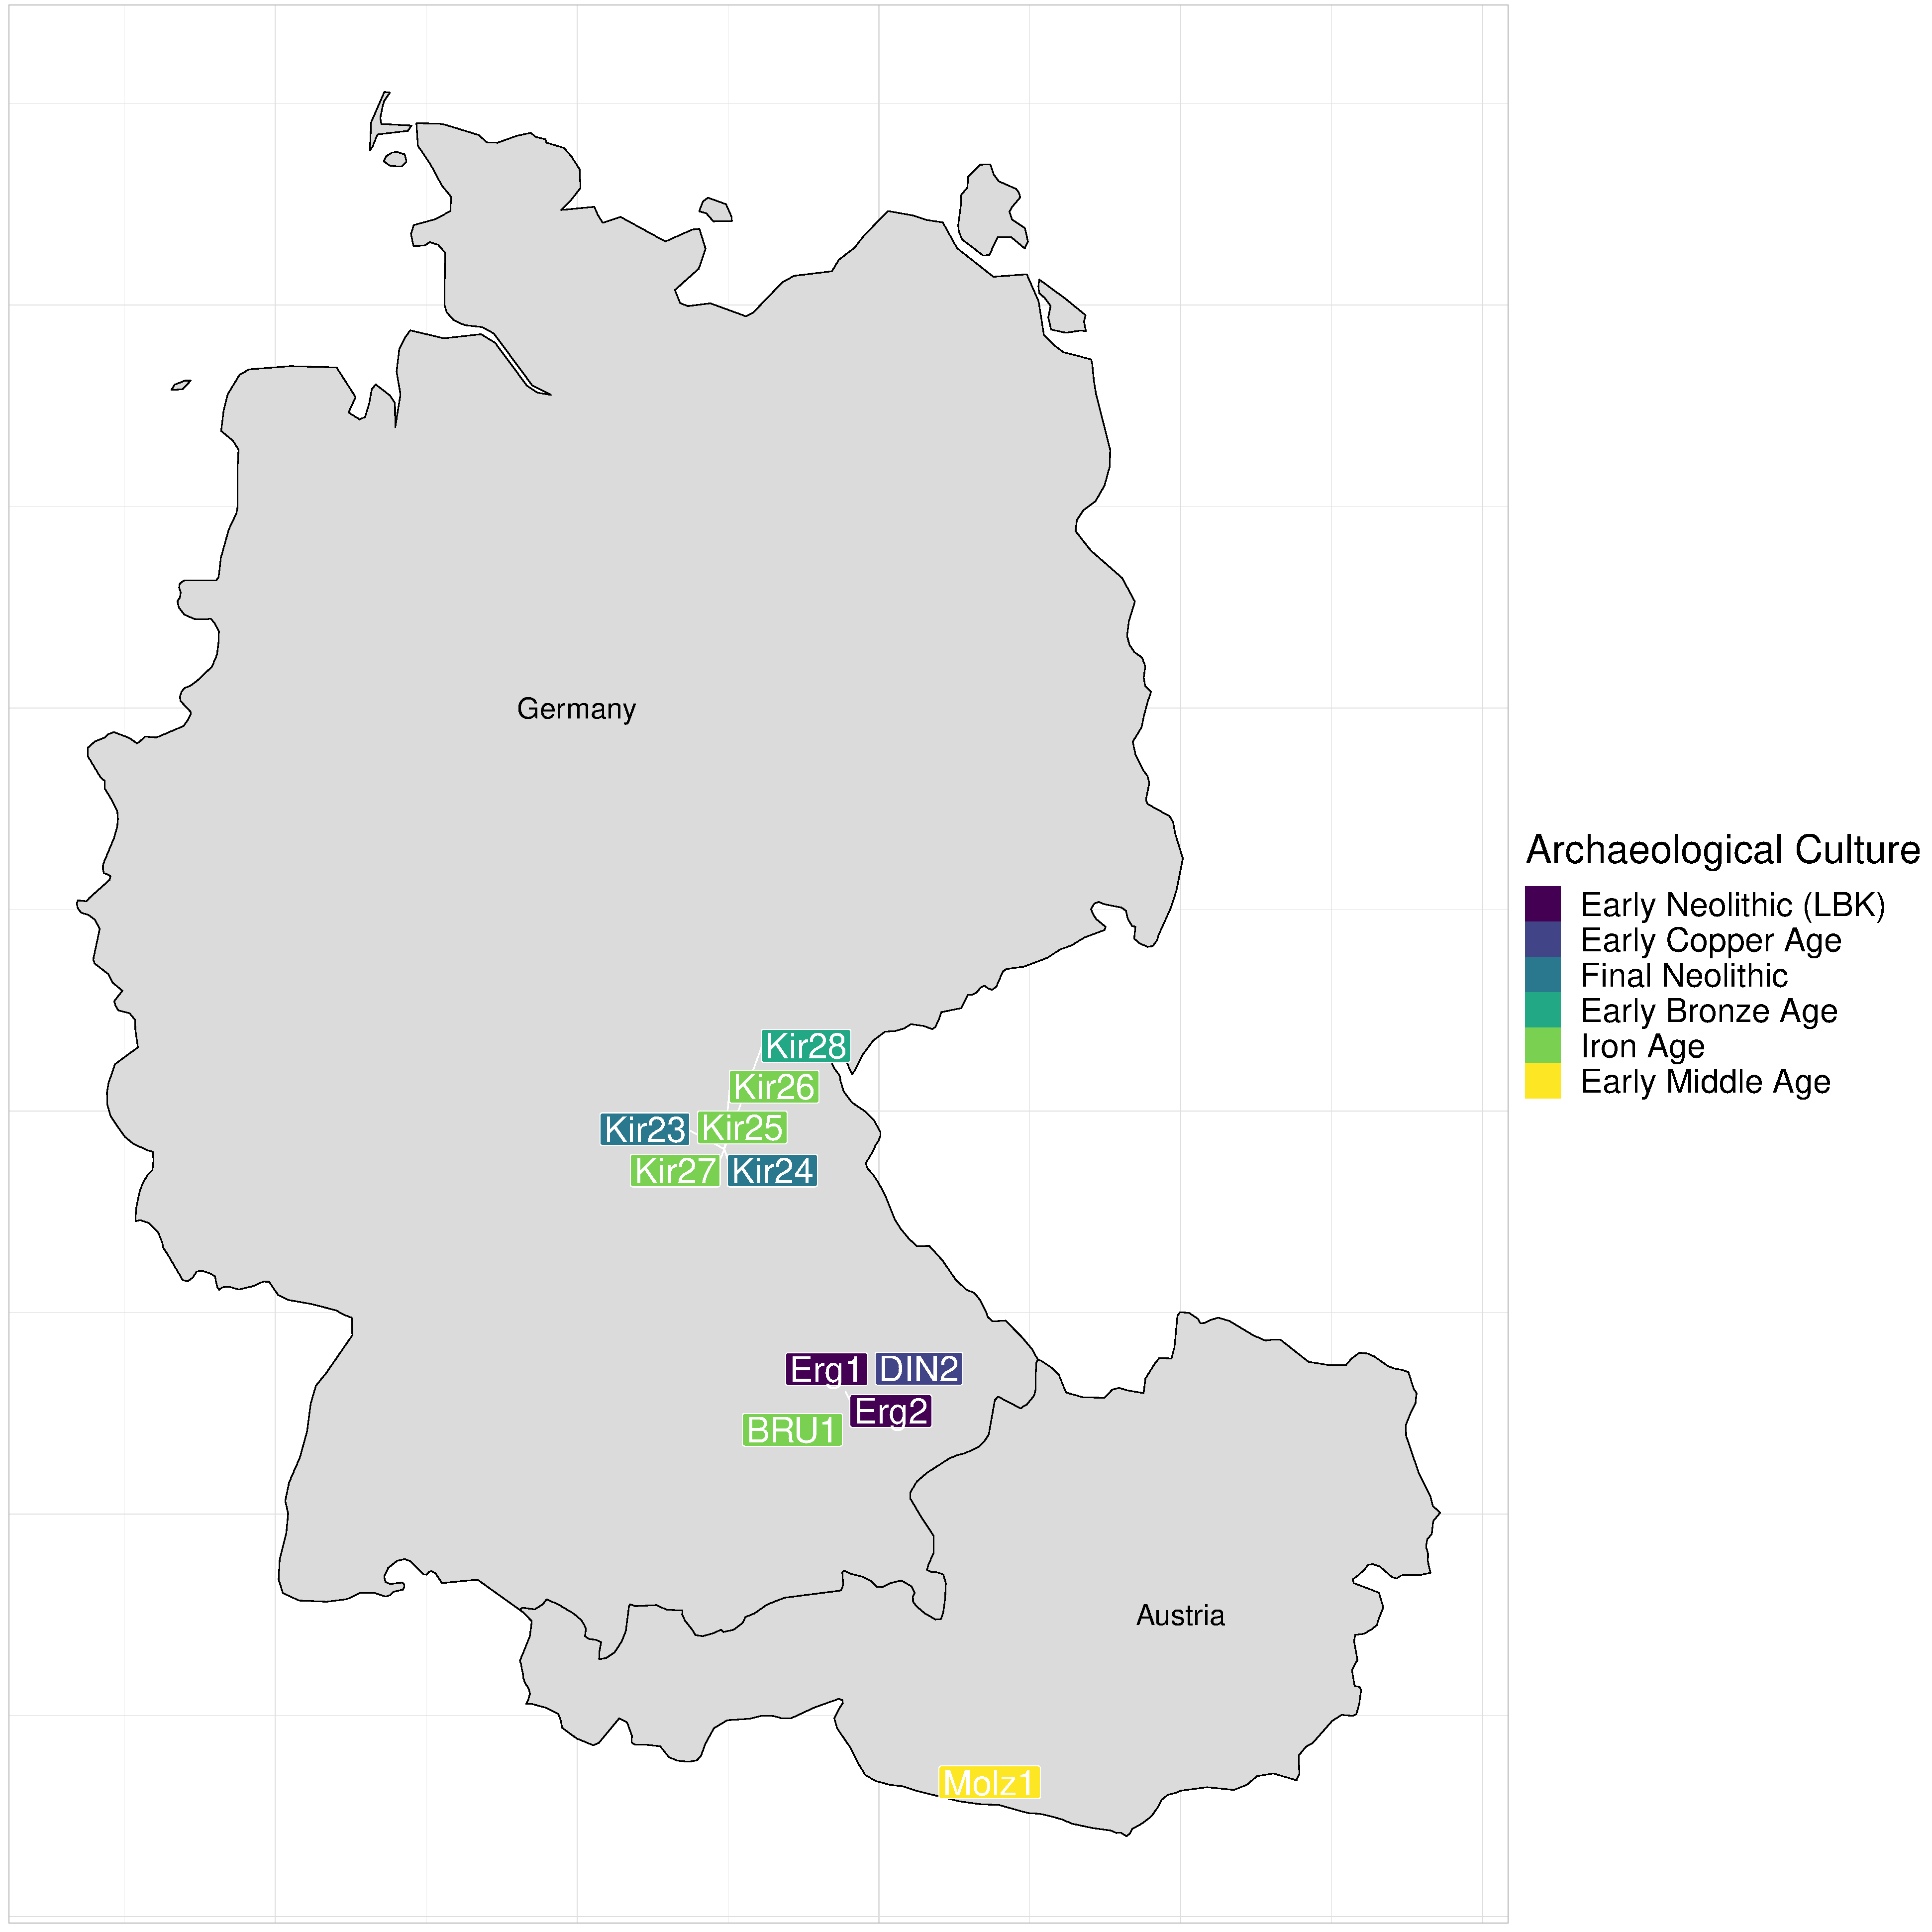
\includegraphics[width=1.0\textwidth]{../images/chapter4/sample_map.pdf}
    \caption{Map of newly sequenced ancient individuals, positioned according to where they were excavated. Colour on label corresponds to archaeological culture which they were found. }
    \label{fig:chapter4_intro_SamplesMap}
\end{figure}

\begin{figure}[htp]
    \centering
    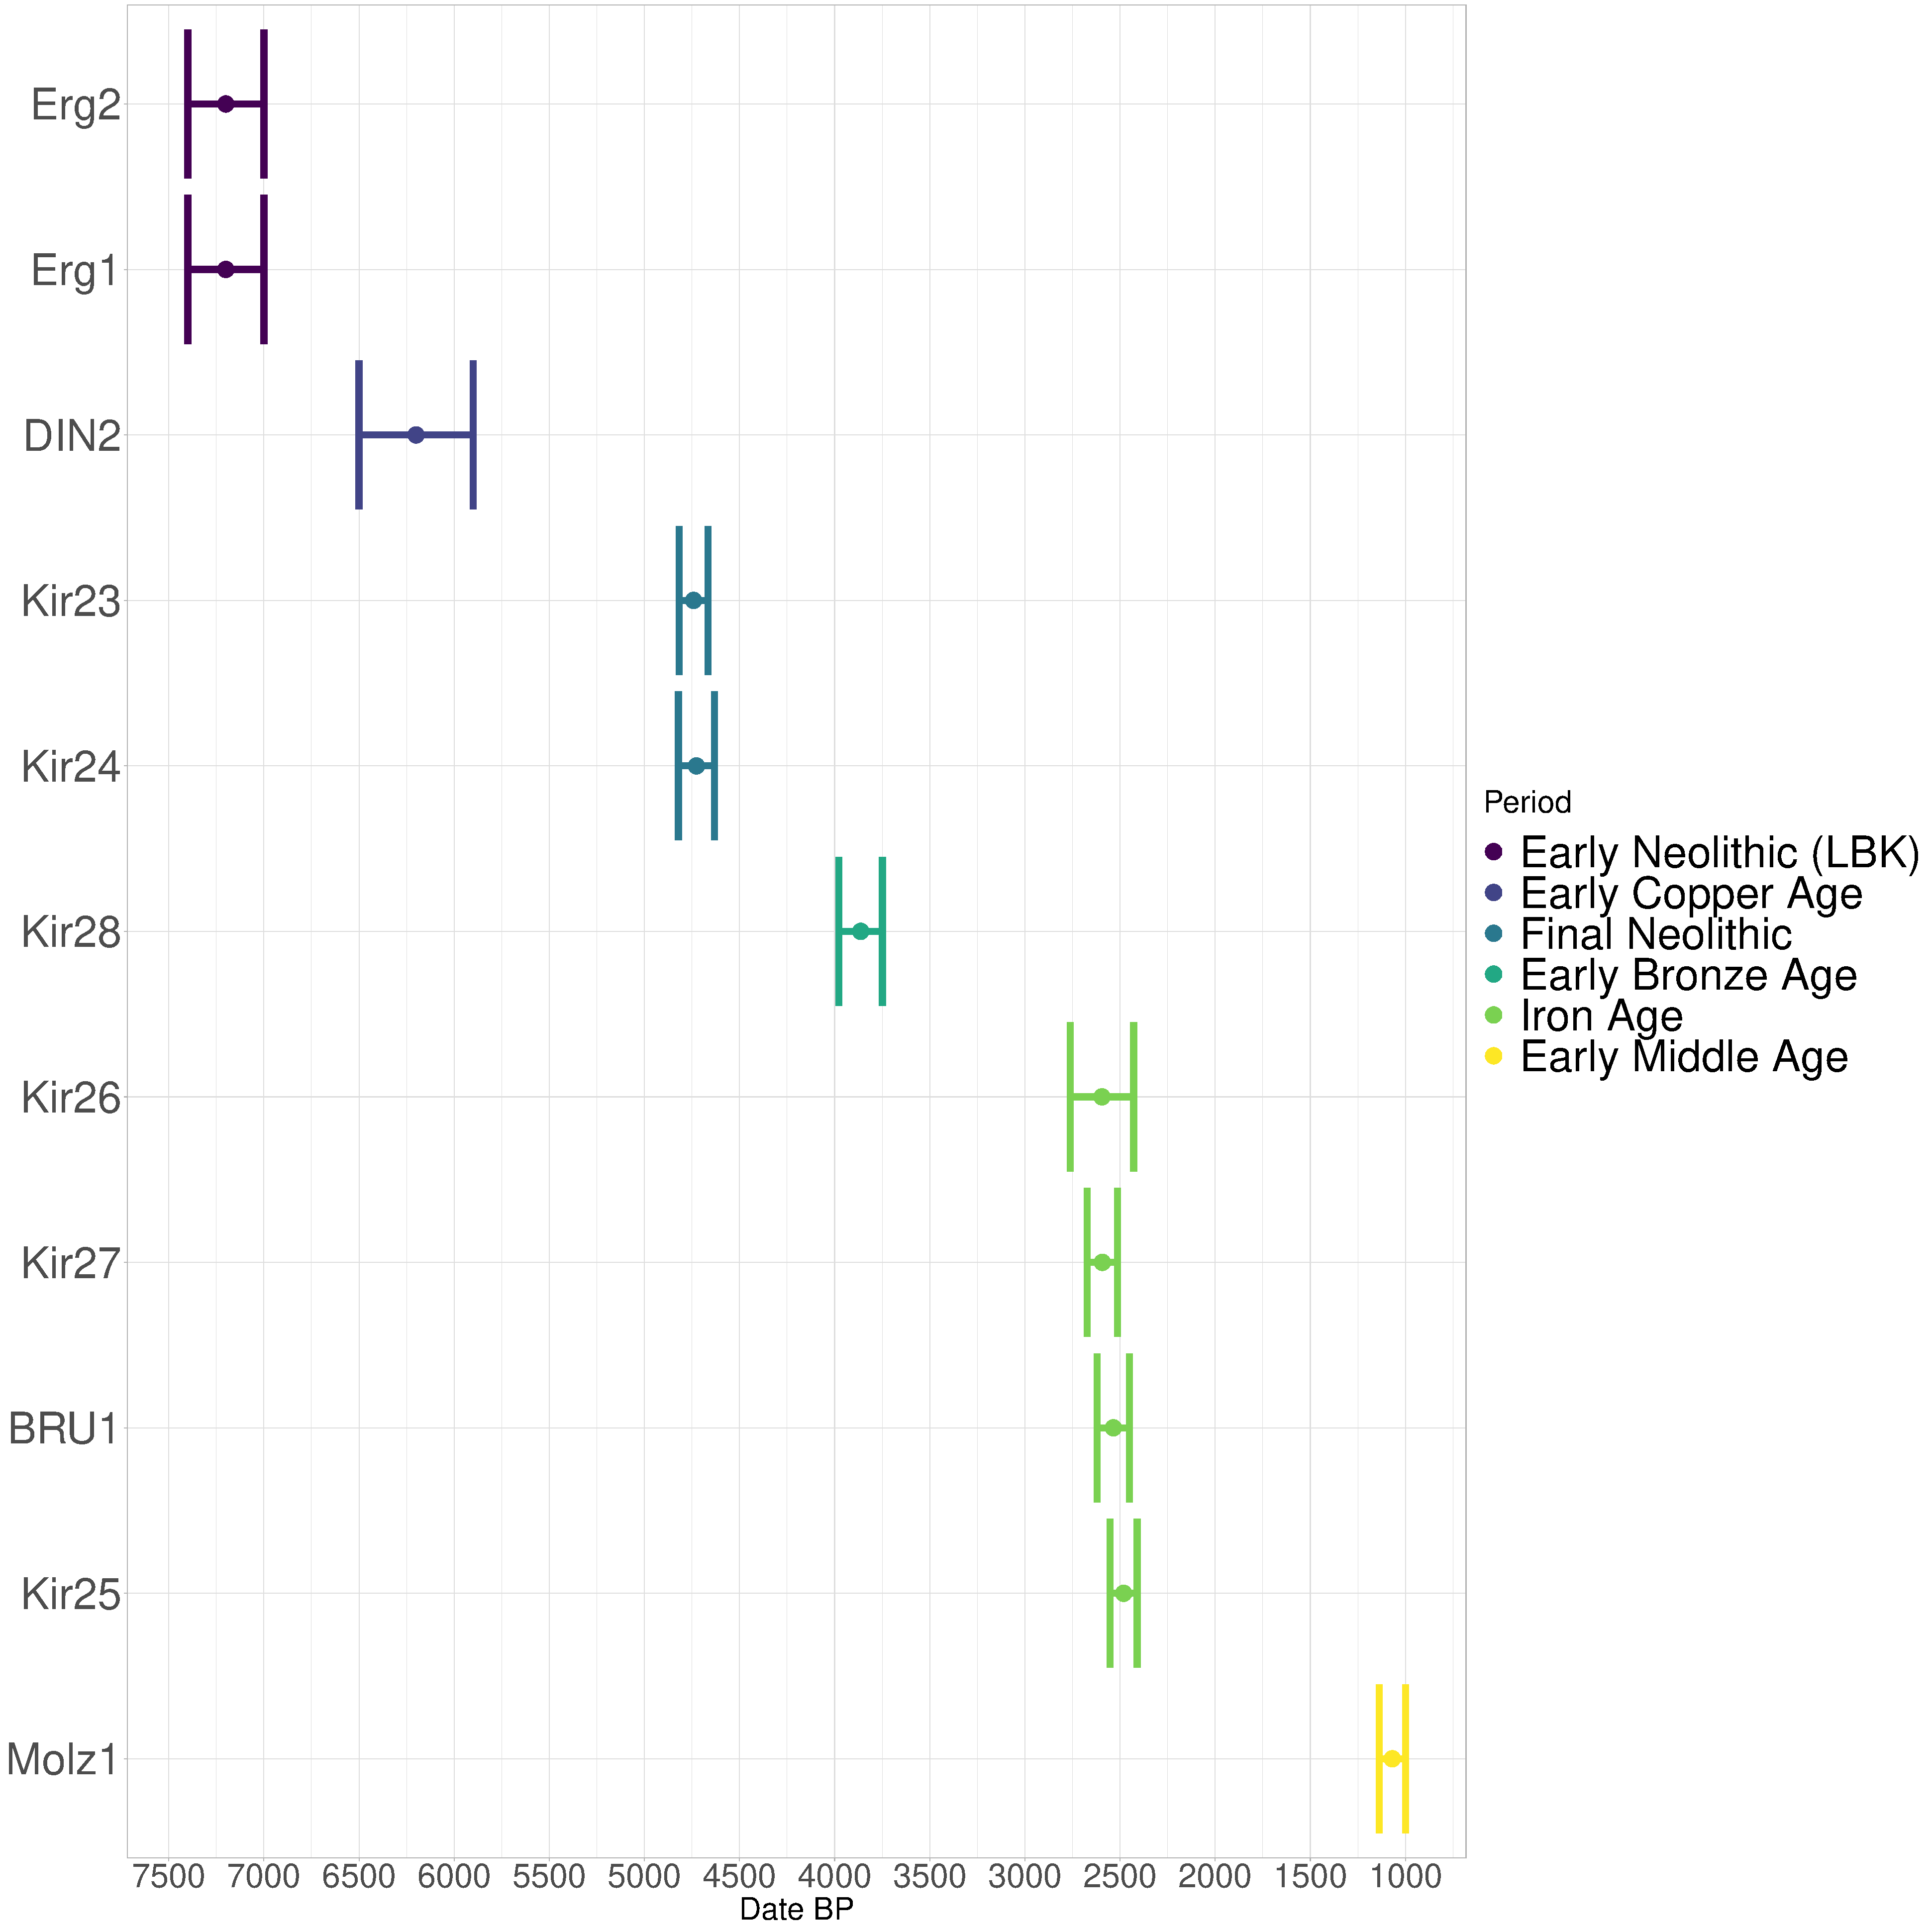
\includegraphics[width=1.0\textwidth]{../images/chapter4/Dates.pdf}
    \caption{Estimated radiocarbon dates for each newly sequenced ancient individual, grouped by archaeological period. Error bars correspond to upper and lower 95\% quantiles of the mean date.}
    \label{fig:chapter4_intro_SamplesDates}
\end{figure}

\begin{table}
\centering
\begin{tabular}[t]{llrrrlr}
\toprule
Sample.ID & Location & Date  & UQ  & LQ  & Period & \thead{Sequencing\\ Depth}\\
\midrule
Erg1 & Ergoldsbach & 5200 (BC) & 5400 & 5000 & Early Neo (LBK) & 4.52\\
Erg2 & Ergoldsbach & 5200 (BC) & 5400 & 5000 & Early Neo (LBK) & 0.71\\
DIN2 & Dingolfing & 4200 (BC) & 4500 & 3900 & Early Copper Age & 1.71\\
Kir24 & Cherry Tree Cave & 2762 (BC) & 2821 & 2632 & Final Neo & 3.98\\
Kir23 & Cherry Tree Cave & 2741 (BC) & 2817 & 2666 & Final Neo & 17.52\\
Kir28 & Cherry Tree Cave & 1863 (BC) & 1977 & 1749 & EBA & 17.30\\
Kir26 & Cherry Tree Cave & 595 (BC) & 762 & 428 & Iron Age & 4.84\\
Kir27 & Cherry Tree Cave & 593 (BC) & 672 & 514 & Iron Age & 16.60\\
BRU1 & Bruckberg & 535 (BC) & 620 & 450 & Iron Age & 11.54\\
Kir25 & Cherry Tree Cave & 481 (BC) & 552 & 410 & Iron Age & 4.55\\
Molz1 & Molzbichl & 1069 (AD) & 1138 & 1000 & Early Middle Age & 13.22\\
\bottomrule
\end{tabular}
\caption{Details of newly sequenced ancient DNA samples. UQ and LQ give upper and lower 95\% quantile estimates for radiocarbon dates. EBA is Early Bronze Age.}
\label{tab:BavariaSampleInfo}
\end{table}

\subsection{Genotype imputation and phasing using GLIMPSE}
\label{sssec:imputationphasingGLIMPSE}

In order to compare the genetic variation in the newly sequenced samples to a reference dataset, I merged them with the 942 ancient samples from the literature detailed in Appendix section \ref{section:AncientReferenceDataset}, resulting in a total of 955 samples in \texttt{.bcf} format with genotype likelihood data at 77,213,942 genome-wide SNPs. 

I followed the recommended GLIMPSE \cite{rubinacci2021efficient} imputation and phasing pipeline (\url{https://odelaneau.github.io/GLIMPSE/tutorial_b38.html}), using the 30x-coverage 1000 genomes dataset \cite{byrska2021high} as a reference panel. This resulted in phased haplotypes and posterior genotype likelihoods for each of the 955 individuals. 

\subsection{Uniparental haplogroups}

To determine the mtDNA haplogroups for each newly sequenced ancient sample, I used Haplogrep (\url{https://haplogrep.i-med.ac.at/}) \cite{weissensteiner2016haplogrep} on the raw \texttt{.fastq} file for each sample. 

\subsection{IBD sharing}

I used hap-IBD \cite{zhou2020fast} to estimate IBD segments greater than 2cM in length between all pairs of ancient individuals above 1.5x coverage (n=466), using the phased output from GLIMPSE as input haplotypes, the genetic maps  from (\url{http://bochet.gcc.biostat.washington.edu/beagle/genetic_maps/plink.GRCh37.map.zip}) and leaving all parameters as default. 

\subsection{plink PCA}

To obtain a broad overview of the ancestry of the newly sequenced individuals in the context of the 942 literature samples detailed in Appendix section \ref{section:AncientReferenceDataset}, I performed PCA on the pre-imputation genotypes using plink2 \cite{chang2015second}. Genotypes were set to missing in an individual if, at that position, they were covered by fewer than two reads. 

I retained the 500,000 markers with the lowest amount of missingness across all samples and LD-pruned the resulting SNPs using the settings \texttt{--maf 0.01} and \texttt{--indep-pairwise 50 5 0.2}. PCA was performed using default settings from plink2.

\subsection{ChromoPainter and fineSTRUCTURE analysis}

To characterise the ancestry of the newly sequenced ancient samples in the context of other ancient individuals, I first selected all newly sequenced samples and literature samples above 1.5x coverage (n=466) and performed an `all-v-all' painting where each sample was painted using all other samples. 1.5x was somewhat arbitrarily chosen as my previous work has shown this is a suitable threshold for the inclusion of samples for ChromoPainter analysis (section \ref{sec:ChromoPainterChap2}); whilst I show 0.5x as the cut-off for coverage-related effects, I chose to be conservative and opt for a higher threshold, given all but one of the 11 newly sequenced samples have average coverage $>1.5$x. I used this painting, hereafter referred to as `ancient' painting, to perform fineSTRUCTURE clustering and tree building on the ancient samples. 

I performed Principle Component Analysis on the coancestry matrix of the `ancients' painting using the \texttt{prcomp\_irlba} function from the irlba R library. To account for the fact that the diagonals of the coancestry matrix are always zeros (as an individual cannot be painted by themselves), I set the diagonal of each row to be the mean of that row, following Lawson et al 2012 \cite{Lawson2012}. Although there were 466 individuals in the `ancients' painting, not all of these were included in the chunklengths PCA. This was because many individuals in that set were not relevant to exploring the ancestry of the Bavarian individuals. For instance, when plotted, samples such as those from the Xiong Nu, a 3rd century BC culture from inner Mongolia, dominate the variation in a PCA to the point where identifying structure between the samples of interest becomes challenging. Therefore I removed 327 individuals based on visual inspection of the first two principal components.

\begin{table}
\centering
\begin{tabular}[t]{lc}
\toprule
Population & \thead{Number of\\samples}\\
\midrule
HB:belorussian & 9\\
HB:bulgarian & 31\\
HB:croatian & 19\\
HB:cypriot & 12\\
HB:french & 28\\
HB:german & 30\\
HB:germanyaustria & 4\\
HB:greek & 20\\
HB:hungarian & 19\\
HB:irish & 7\\
HB:lithuanian & 10\\
HB:mordovian & 15\\
HB:northitalian & 12\\
HB:norwegian & 18\\
HB:polish & 17\\
HB:romanian & 16\\
HB:russian & 25\\
HB:scottish & 6\\
HB:siciliane & 10\\
HB:southitalian & 18\\
HB:spanish & 34\\
HB:tsi & 98\\
HB:tuscan & 8\\
HB:ukrainian & 20\\
HB:welsh & 4\\
HB:westsicilian & 10\\
\bottomrule
\end{tabular}
\caption{Name of population and number of samples used in the present-day ChromoPainter, MOSAIC and qpAdm analyses. All populations from the HellBus dataset.}
\label{tab:BavariaModernSamples}
\end{table}

To determine the genetic similarity between the newly sequenced ancient samples and present-day populations, I performed an `all-v-all' painting using a selected group of 26 present-day European populations (Table \ref{tab:BavariaModernSamples}) from the HellBus dataset (described in Appendix section \ref{section:MSPOBIHellBus}) and the 11 newly sequenced ancient individuals, hereafter referred to as `present-day painting'.

I applied fineSTRUCTURE (v0.0.5)\cite{Lawson2012} to cluster the chunkcounts ChromoPainter output for the `ancients' painting. fineSTRUCTURE assigns individuals to clusters, estimates the  number of clusters and builds a dendrogram of genetic similarity based on a tree-building algorithm. This is particularly useful when combining many samples from different studies, as is the case with the `ancients' painting; the population label identifiers used by different studies may not be consistent with one another. Therefore, we can use fineSTRUCTURE groupings as population labels rather than group labels. fineSTRUCTURE was first run in MCMC mode using 1,000,000 burn-in MCMC iterations and 2,000,000 main MCMC iterations. It was then run in tree-building mode (\texttt{-m T}) using 100,000 burn-in and 100,000 main iterations. 

Tree figures, coancestry matrix figures and principle component plots were generated using the fineSTRUCTURE R library \url{(https://people.maths.bris.ac.uk/~madjl/finestructure/FinestructureRcode.zip)}.

\subsection{SOURCEFIND} \label{sec:ch4_SOURCEFIND}

I used SOURCEFIND \cite{Chacon-Duque2018} to infer the proportions of ancestry by which each newly sequenced ancient individual is most related to a set of surrogate populations. While this method does not explicitly attempt to identify admixture, in contrast to e.g. ALDER \cite{LohAlderAdmixture} or GLOBETROTTER \cite{Hellenthal2014}, it can reflect admixture proportions \cite{Chacon-Duque2018} but more generally reflects recent ancestry sharing patterns.

The first analysis used the ancients painting and only three surrogates: Western Hunter-Gatherers, Neolithic farmers from Anatolia and Yamnaya, to mimic previous research suggesting many ancient Europeans descend from the mixture of three sources well-represented by these groups \cite{Lazaridis2014}. The second analysis attempted to characterise more fine-scale ancestry patterns, by modelling each target ancient individual (using the same ancients painting) as a mixture of all sampled ancient populations above 1.5x coverage (n=466) that had an average sample age no more than 100 years younger than that of the target individual. The third analysis used the ``modern'' painting and formed each ancient individual as a mixture of all present-day populations shown in Table \ref{tab:BavariaModernSamples}. For each of these analyses, I found the mean and 95\% credible interval of ancestry estimates across 2,000,000 posterior samples combined from three independent SOURCEFIND runs that each sampled every 10,000 MCMC iterations after discarding the first 10,000 MCMC iterations as ``burn-in''.


\subsection{MOSAIC admixture analysis}

I inferred admixture events, dates and proportions in newly sequenced ancient samples using MOSAIC, a haplotype-based method \cite{MOSAIC_2019}. While MOSAIC cannot infer multiple pulses of admixture from the same admixing sources as GLOBETROTTER \cite{Hellenthal2014} can, in theory it is unlikely we would have adequate power to identify such multiple pulses when analysing only a single ancient sample, as is the case in this study. Furthermore, the `painting' step and admixture inference step in MOSAIC are combined, providing a simpler pipeline and more flexible assignment of different surrogates relative to GLOBETROTTER (i.e.\ the set of surrogates can be changed without repainting the samples).

I performed two MOSAIC analyses that correspond to two of the SOURCEFIND analyses described in Section \ref{sec:ch4_SOURCEFIND}. First, I performed an `ancient surrogates' analysis where the all ancient samples above 1.5x coverage (n=466) were used as surrogates to admixing sources. I used the fineSTRUCTURE groupings to categorise ancient samples into surrogate populations. Second, I also performed a `present-day surrogates' analysis where a selected set of present-day populations (Table \ref{tab:BavariaModernSamples}) were used as surrogates. While using present-day populations to reflect ancestry patterns in ancient individuals may be counter-intuitive, the larger sample sizes and larger variety of present-day populations can provide more clean results relative to using ancients

I ran MOSAIC using default settings, assuming two or three admixing sources per target individual/population. For populations with more than one sampled individual, MOSAIC provided bootstrap-based 95\% confidence quantiles around date estimates. MOSAIC also estimates $f_{st}$ between the set of surrogates and the estimated `true' mixing source, which is useful when a close proxy for the `true' mixing source is not available

\subsection{F-statistics}

Many of the relevant samples in the literature were of very low coverage ($<0.1$). As my work in section \ref{sec:ChromoPainterChap2} indicated that samples with less than 0.5x coverage cannot reliably be analysed using ChromoPainter, I also used F-statistics \cite{Patterson2012} that are mostly robust to coverage related effects \cite{AssessingqpAdm}. In particular I used Admixtools \url{(https://uqrmaie1.github.io/admixtools)} to analyse 942 individuals from 143 populations (Appendix section \ref{section:AncientReferenceDataset}, including many low-coverage samples from relevant LBK cultures presented in Rivollat et al (2020) that would not have been suitable for use with ChromoPainter \cite{rivollat2020france}. This analysis also incorporated 2280 present-day individuals from 144 populations from the HellBus dataset as putative ancestry surrogates for tested ancient individuals. Populations shown in Table \ref{tab:BavariaModernSamples}. 

For the input to ADMIXTOOLS, I used the genotyped imputed from GLIMPSE, as it has been shown that using imputed markers reduced reference bias relative to using pseudo-haploid markers \cite{Martiniano2017}. I then used the $f_{4}$ branch test to test whether two populations form a clade relative to two other populations. For example, the expected value of $f_{4}(french,german;yoruba,mbuti)$, which tests whether \{french,german\} form a clade relative to \{yoruba,mbuti\}, should not give a score significantly different to zero. In contrast, exchanging $french$ with $yoruba$ would yield a significantly positive $f_4$ scores, with strength of evidence to reject the null ($f_4 = 0$) measured using standardised $Z$-statistics.

I also used the $f_3$ test, denoted $f_{3}(A,B;C)$, to (i) estimate the branch length between $A$ and $B$ after their divergence from $C$, or (ii) test whether $C$ descends from an admixture event between sources represented by $A$ and $B$. The latter can occur if $C$ has a substantial number of SNPs with allele-frequencies which are intermediate between $A$ and $B$.

Finally, I used qpAdm to infer ancestry proportions, following the protocol described in Olalde et al (2018) by choosing the following populations/samples as outgroups: \textit{Mota}, \textit{Kostenki14}, \textit{papuan}, \textit{han}, \textit{hannchina}, \textit{mbutipygmy}, \textit{sannamibia}, \textit{yakut}. These outgroups were suitable for use in investigating ancient Eurasians, since they are asymmetrically related to many ancient populations, but do not show evidence of recent gene flow with them. 

\section{Results}

\subsection{Broad-scale ancestry changes in Bavaria reflect those found elsewhere in Europe}

The newly sequenced samples from the Early Neolithic (Erg1 and Erg2, approx 5200BC) and Copper Age (DIN2, approx 4200BC) cluster with other published sampled from European Neolithic on the plink2 PCA (Fig. \ref{fig:plink_PCA}). As in previously reported PCA results \cite{Lipson2017b}, the earliest Neolithic samples, from Anatolia and Greece, and who are thought to be the source population from which all subsequent Neolithic farmers derive \cite{Hofmanova2016, Haak2010, haak2005ancient, bramanti2009genetic, Lazaridis2014}, are  positioned at the end of the cluster farthest away from the hunter-gatherer samples (for example, WHG on Fig. \ref{fig:plink_PCA}). This likely reflects the fact that they are unadmixed with respect to the later Neolithic samples. As the Neolithic progressed, farmers from the near-east mixed with local hunter-gatherer groups in central Europe \cite{Lipson2017b} and acquired local hunter-gatherer ancestry. Accordingly, these samples are shifted away from the earlier Neolithic samples towards the hunter-gatherers. With this in mind, the position of the new Early Neolithic sample Erg1, shifted north away from the contemporaneous sample Erg2, is suggestive of hunter-gatherer admixture. 

There are four key observations from the Figure \ref{fig:plink_PCA} PCA regarding the new samples:

\begin{enumerate}
\item The two Late Neolithic individuals are genetically separate, with Kir24 positioned close to Yamnaya and Kir23 clustering with Neolithic Europeans.
\item The Bronze Age sample Kir28 clusters with other European Bronze Age samples
\item The four Iron Age samples (Kir25, Kir26, Kir27 and BRU1) cluster towards the Neolithic individuals and other European Iron Age samples
\item The three Medieval period samples (Alh1, Alh10, Molz1) cluster with the Bronze Age sample Kir28 instead of the Iron Age samples.
\end{enumerate}

\begin{figure}[htp]
    \centering
    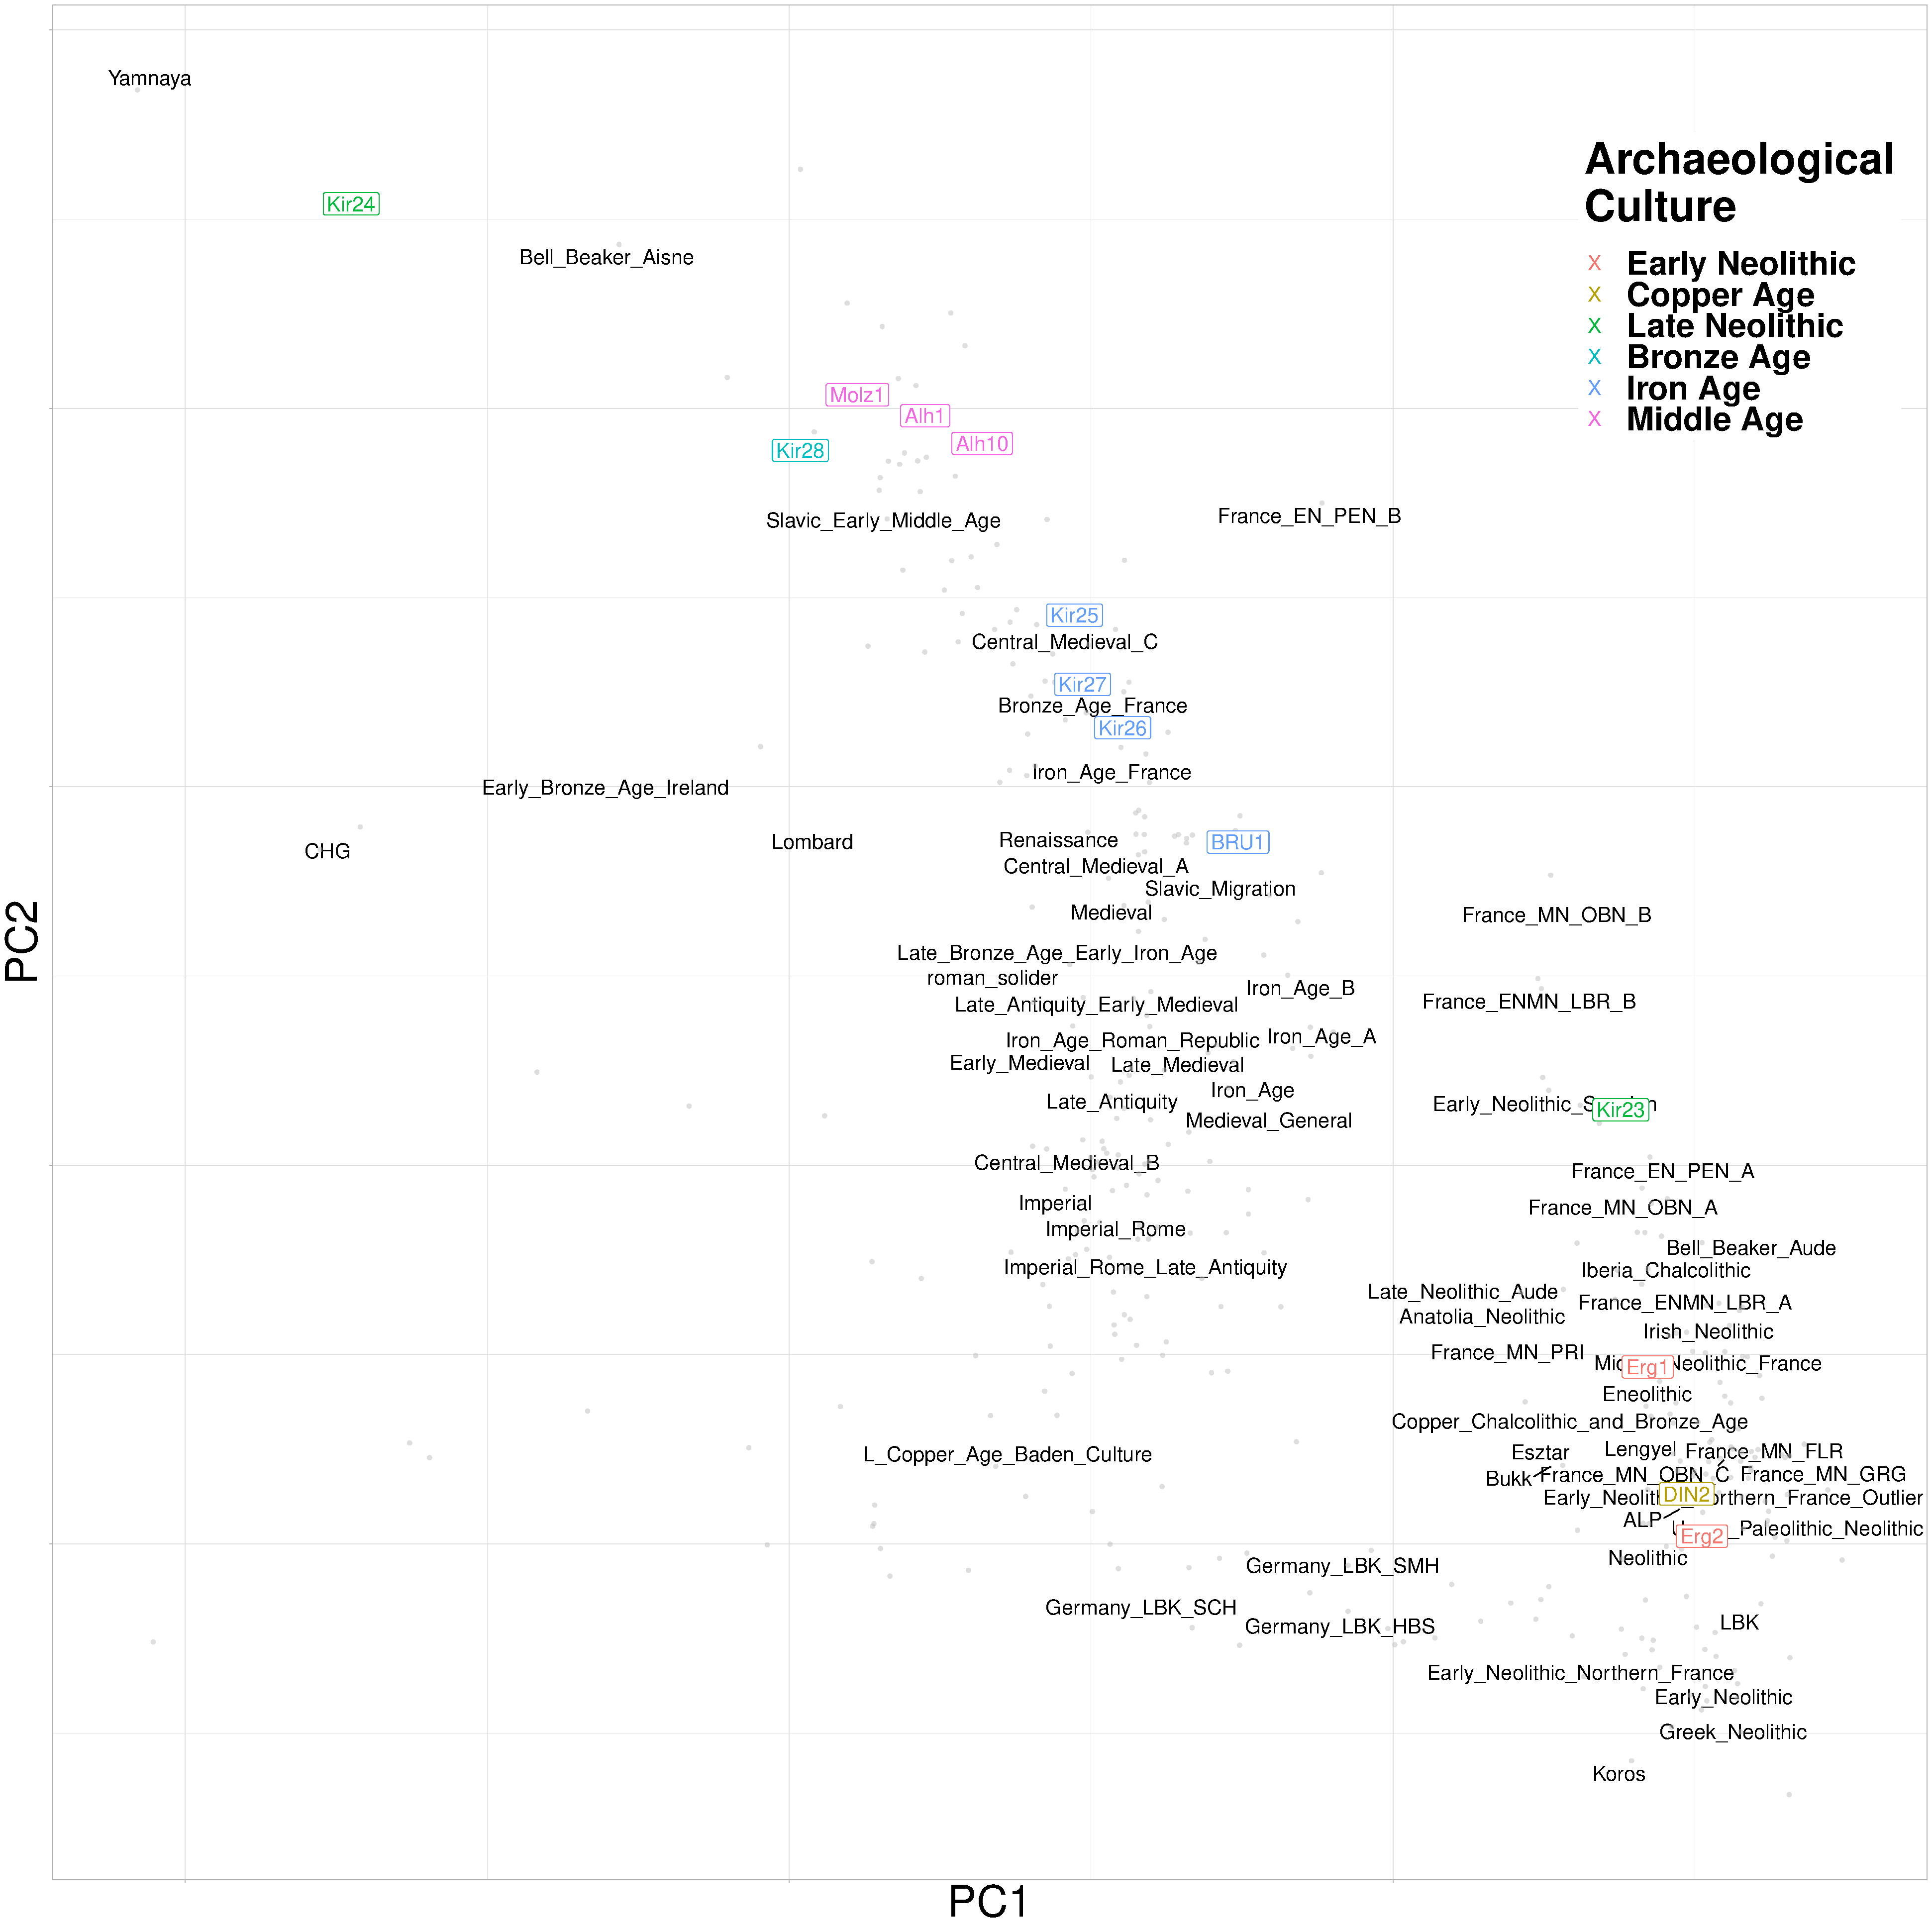
\includegraphics[width=1.0\textwidth]{../images/chapter4/plink_PCA.pdf}
    \caption{Principle component analysis of pre-imputation genotypes using plink2. Grey points indicate principle component coordinates for each sample. Black text indicated mean principle component coordinates for all individuals within that group. Coloured labels represent newly sequenced ancient samples.}
    \label{fig:plink_PCA}
\end{figure}

\subsection{Early Neolithic}

\begin{figure}[htp]
    \centering
    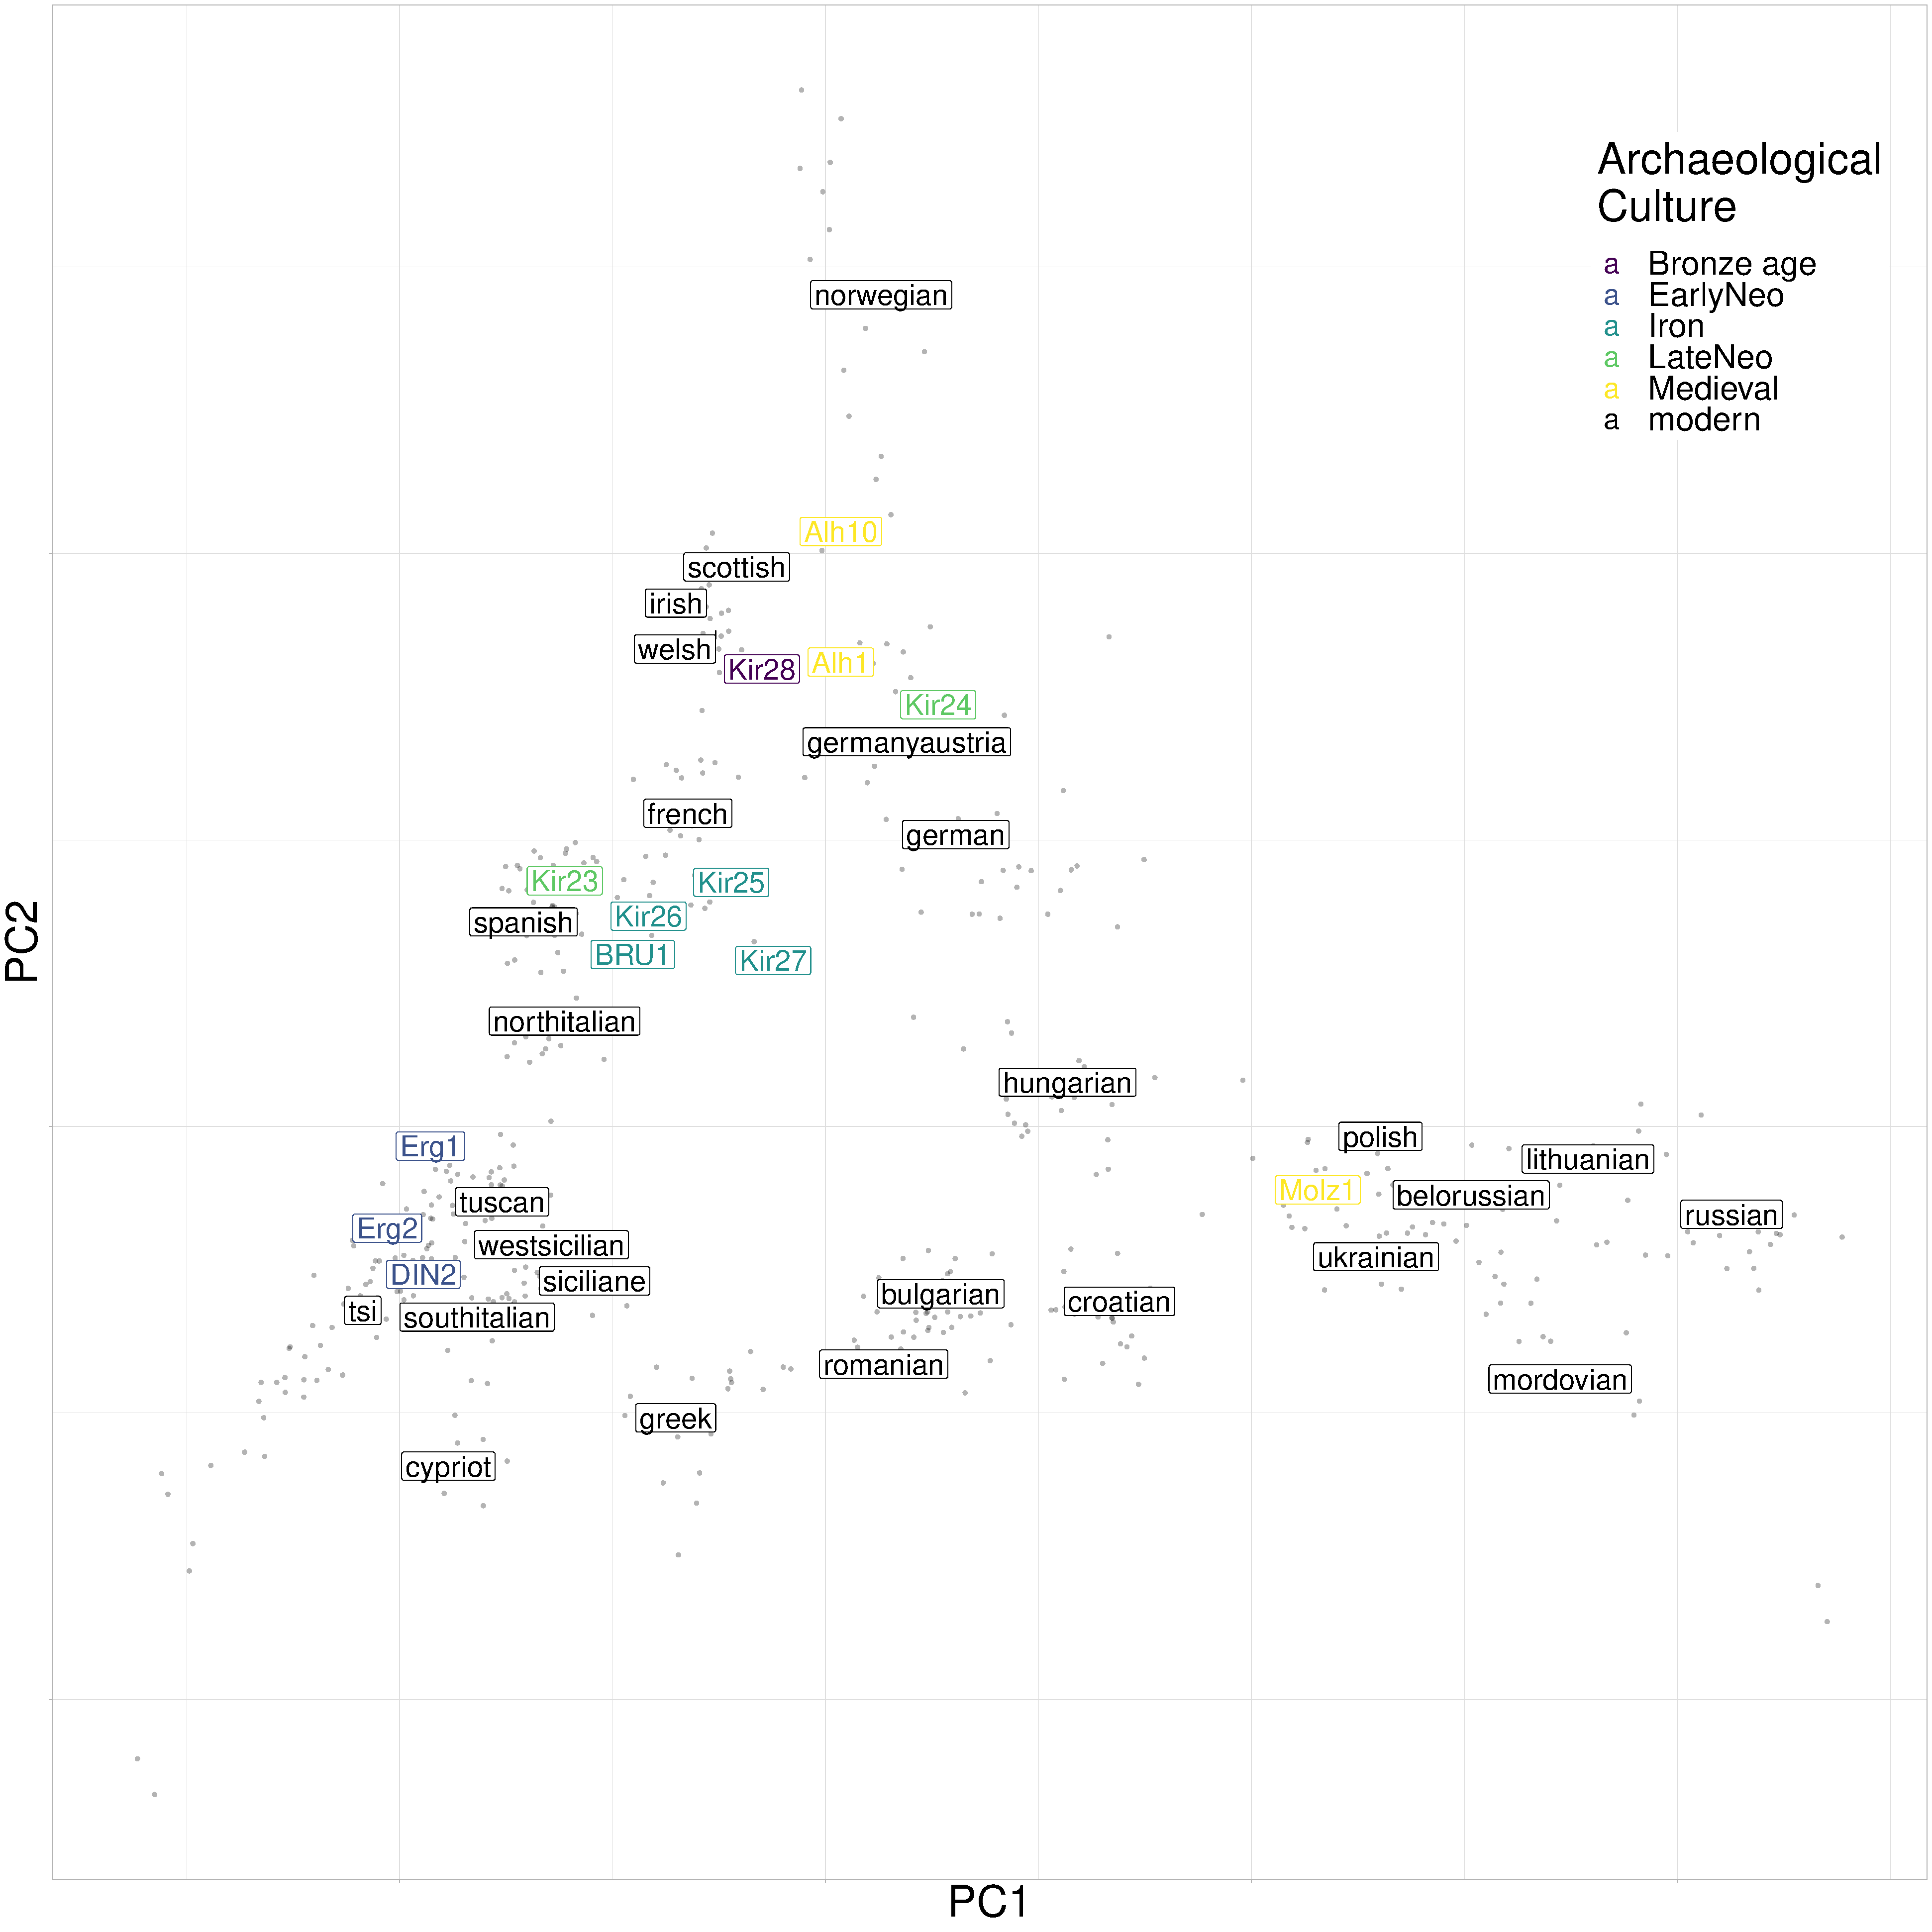
\includegraphics[width=1.0\textwidth]{../images/chapter4/chunklengths_moderns_ancients_PCA.pdf}
    \caption{Principle component plot of newly sequenced ancient samples and reference modern individuals performed using the finestructure library. Green labels correspond to Migration Era samples, red labels correspond to Early Middle Age samples and white labels correspond to reference populations. The position of each reference label is the mean PC coordinates of all individuals within that population. Transparent coloured points correspond to present-day individuals.}
    \label{fig:chunklengths_moderns_ancients_PCA_bav}
\end{figure}

The three Early/Middle Neolithic samples, Erg1, Erg2 and DIN2, all display a strong affinity to Anatolian farmers, consistent with the prevailing theory that near-eastern farmers were responsible for the spread of early agricultural technology across Europe, and that all Neolithic farmers share recent common ancestry \cite{Haak2010, haak2005ancient, bramanti2009genetic, Lazaridis2014}. fineSTRUCTURE  grouped Erg1 with two samples from Upper Palaeolithic/Neolithic Italy and DIN2 with Early/Middle Neolithic samples from Germany, Greece, Anatolia and Hungary. Despite their age, the genetic variation of the Early Neolithic samples falls well within the variation of present-day individuals; when painted using present-day samples, the three Early Neolithic individuals cluster with present-day Italians, consistent with findings from previous research \cite{Lazaridis2014, Haak2015} (Fig. \ref{fig:chunklengths_moderns_ancients_PCA_bav}). Erg1 was assigned to mtDNA haplogroup K which has been found in Neolithic and pre-pottery sites across Europe \cite{Hofmanova2016, fernandez2014ancient} and Western Asia \cite{Lazaridis2016, Mathieson2015}. 

Erg1 is from the \textit{Linearbandkeramik} (LBK) culture and is speculated to have belonged to the first wave of immigrants carrying farming technology from south-eastern Europe or Anatolia into central Europe. DIN2 is from a nearby site, around 500 years more recent, and is thought to potentially belong to a second wave of farmers who migrated along the Danube. It is unclear to what extent these different waves corresponded to populations with different ancestries.  

When painted using 465 ancient samples from the literature and the newly sequenced samples, Erg1 had the lowest $TVD$ ($TVD$ is a distance metric based on ChromoPainter copyvectors; calculation and justification outlined in Appendix section \ref{sec:appendixTVD}) with DIN2, supporting the hypothesis that they were from similar source population. DIN2  has the lowest $TVD$ with NE5, NE4 and NE7, samples assigned to Middle and Late Neolithic cultures on the Hungarian plane, and was assigned to mitochondrial haplogroup (J1C) alongside NE4 and NE5. Both the autosomal and mtDNA link to Neolithic Hungary supports the hypothesis that DIN2 migrated along the Danubian route.   

To explicitly test whether Erg1 and DIN2 group together to the exclusion of other ancient samples and therefore, whether they likely originated from a similar source population, I performed $f_{4}$ tests in the form of $f_{4}(W=Erg1, X=DIN2; Y=test, Z=Mbuti)$, where $test$ is 143 ancient populations used in the F-statistics analysis. This tests whether Erg1 and DIN2 form a clade to the exclusion of $test$ or not. Of the 143 comparisons, only the population labelled as WHG had a $|Z|>3$, ($Z=3.057$), suggesting that Erg1 and DIN2 originate from the same local population. Whilst qpAdm and SOURCEFIND results show that both Erg1 and DIN2 contain a small but significant proportion of hunter-gatherer ancestry, it is not clear whether the result of the $f_{4}$ test is due to admixture or statistical chance; one test with $|Z|>3$ may be expected when doing 143 tests, even if the null is true.

To determine whether Erg1 showed increased genetic similarity to local farming populations, I also performed combinations of $f_{3}$ in the form of $f_{3}(A=Erg1, B=test, C=Mbuti)$, where $test$ iterates across 143 ancient populations. This tests the branch length, or the amount of genetic drift that has occurred on the branch shared by Erg1 and $test$ since their divergence from an outgroup (Mbuti). The sample/population with the highest $f_{3}$ statistic was NE7, a sample from 4,360 – 4,490 BC and the Lengyel culture (a Neolithic culture centered on the Danube River, known to be an offshoot of the LBK culture Erg1 belonged to). On the other hand, DIN2 shows a clear affinity to samples from Neolithic France.

My dataset included data from several other LBK populations local to Erg1 and DIN2; samples from Schwetzingen, Stuttgart-Mullhausen and Halberstadt. These samples appear to form a distinct cluster on the plink PCA and are shifted away from the primary cluster of Neolithic individuals and towards samples from the Anatolian Bronze Age and Baden Culture (a central European Chalcolithic culture) (Fig. \ref{fig:plink_PCA}). I wanted to know which LBK population Erg1 and DIN2 were closest to. I found strong evidence ($|Z| = 7.97$) that Erg1 shared more alleles with LBK populations from Schwetzingen than with Stuttgart-Mühlhausen, suggesting the early LBK populations showed relatively fine-scale geographic structure. Given the lack of Hunter Gatherer ancestry in the Rivollat LBK samples, this structure seems unlikely to be driven by variable amounts of Hunter-Gatherer admixture (Fig. \ref{fig:HG_ancestry_Neolithic}).


\subsection{Variable amounts of local hunter-gather ancestry in Neolithic farmers indicates a structured population}

Prior research has shown that admixture occurred between newly arrived farming immigrants from Anatolia and local hunter-gatherers \cite{Gamba2014, Haak2015, mathieson2018genomic, gonzalez2017paleogenomic, Lipson2017b}. The position of Erg1 on the PCA, shifted slightly north towards the majority of the Bronze Age samples, suggests that it may have a component of Hunter-Gatherer ancestry. Indeed an $f_{3}$ admixture test, using $f_{3}(A=Castelnovian Mesolithic, B=LBK; C=Erg1)$ to test for admixture in $C$ from two sources related to surrogates $A$ and $B$, yielded a significantly negative result $(|Z|=4.25)$, as expected in the case of admixture \cite{Patterson2012}. Furthermore, qpAdm also concluded that Erg1 can be modelled as a mixture of Anatolia Neolithic (66\%, se=8.1) and WHG (33\%, se=8.1) (Fig. \ref{fig:HG_ancestry_Neolithic}). In contrast, qpAdm modelled Erg2 as descending solely from sources related to Anatolian Neolithic farmers.  MOSAIC also inferred admixture in Erg1, dated to 5.3 generations prior to it sample date (i.e. approximately 5288 years ago), between WHG and Anatolia Neolithic sources. I caution that the admixture date may be unreliable due to only targeting a single individual, and given MOSAIC bootstraps over individuals, it was not possible to obtain confidence intervals around admixture date. 

\begin{figure}[htp]
    \centering
    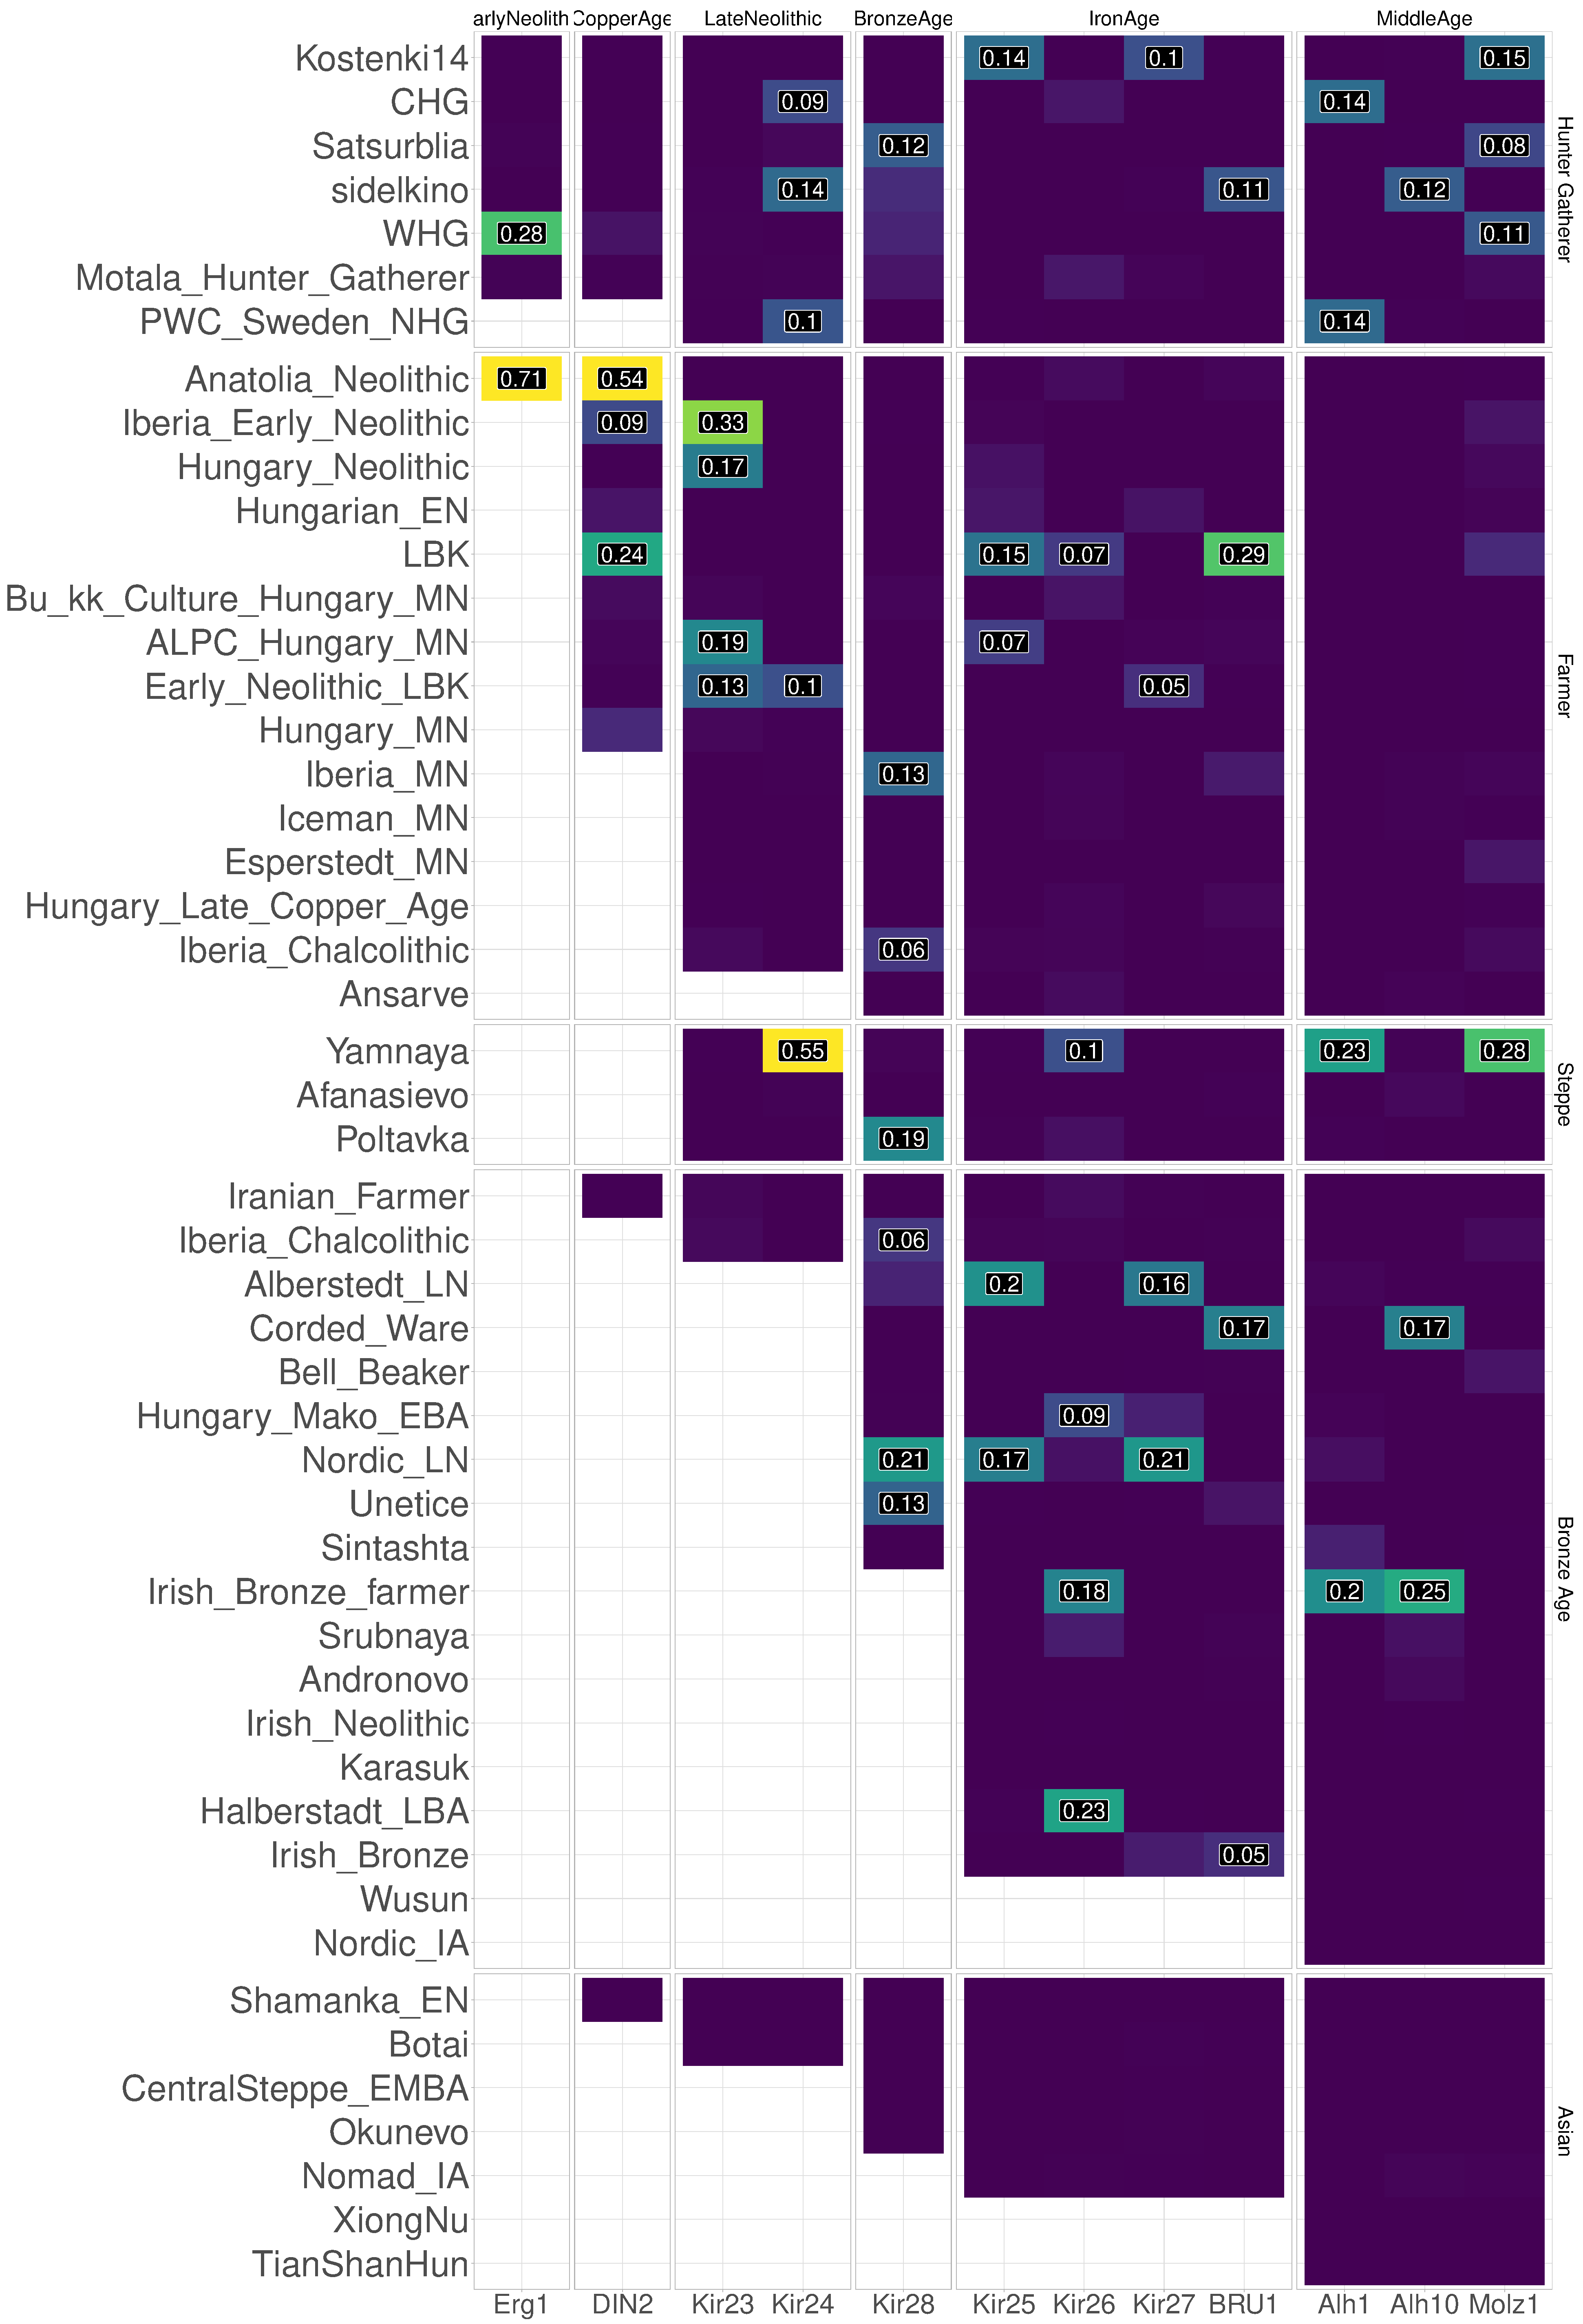
\includegraphics[width=1.0\textwidth]{../images/chapter4/SOURCEFINDheatmapOlderSurrogates_2.pdf}
    \caption{SOURCEFIND ancestry proportion estimates for all newly sequenced target samples (vertical columns). Target samples are grouped by archaeological age. Surrogate populations are represented as horizontal rows and also grouped into archaeological culture. Each target was modeled as a mixture of only populations which are dated to being older or contemporaneous as the the target. Numbers within each cell correspond to the ancestry proportion estimate.}
    \label{fig:chapter4resultsSFheatmapolder}
\end{figure}


Estimated Hunter-gatherer related ancestry in Erg1 ranged from 18-38\% among MOSAIC (Fig. \ref{fig:Erg1_MU_matrix}) and qpAdm (Fig. \ref{fig:HG_ancestry_Neolithic}), with SOURCEFIND inferring 27.2\% (se=1.41) when using six surrogates \{Anatolian Neolithic, Loschbour, LaBrana, Bichon, and the two `Iron Gates' samples\}. MOSAIC indicated the cluster of Italian hunter-gatherers as the closest population to the true mixing source (Fig. \ref{fig:Erg1_MU_matrix}). However, SOURECFIND indicated Iron Gates individuals from Serbia as the largest contributors of hunter-gatherer related ancestry.


\begin{figure}[htp]
    \centering
    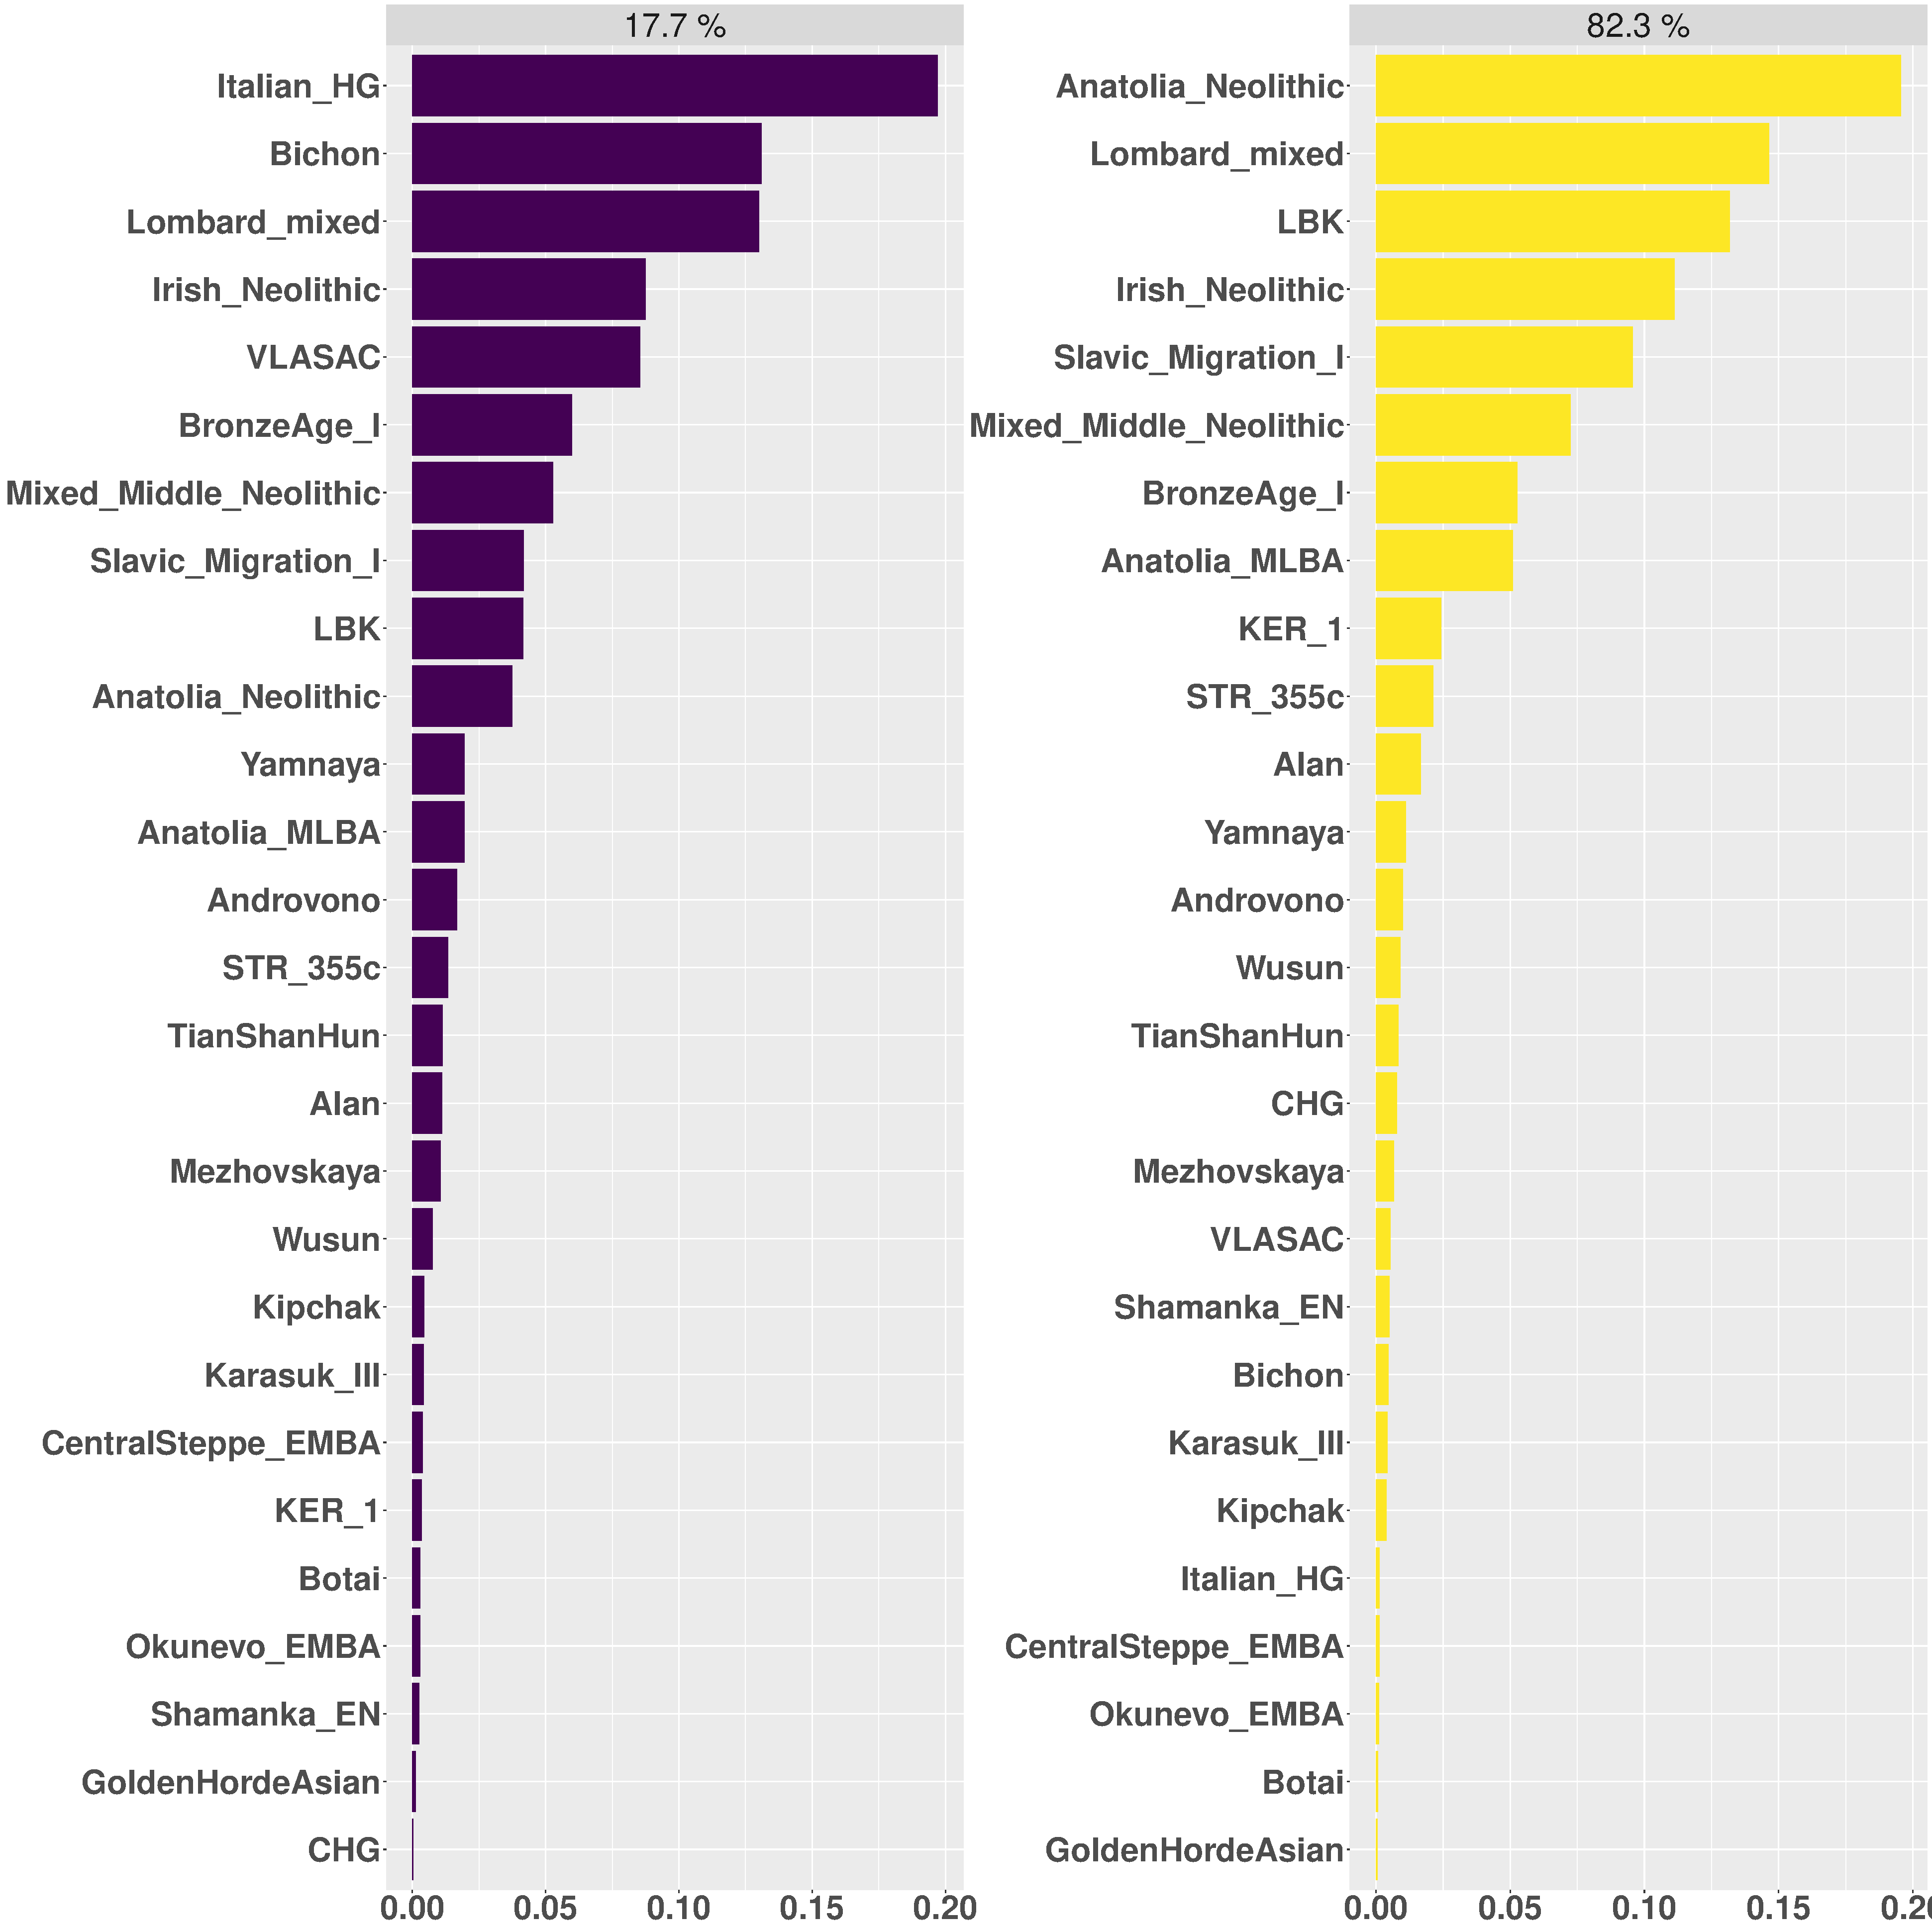
\includegraphics[width=1.0\textwidth]{../images/chapter4/Erg1_MU_matrix.pdf}
    \caption{Copying matrix plot for sources in 2-way admixture event for Erg1. Each panel represents one of the 2 mixing sources. Labels above each panel gives the proportion that mixing source contributed to the Early Middle Age samples. Length of the bars within each panel represent the amount that mixing source copied from a particular population.}
    \label{fig:Erg1_MU_matrix}
\end{figure}



\begin{figure}[htp]
    \centering
    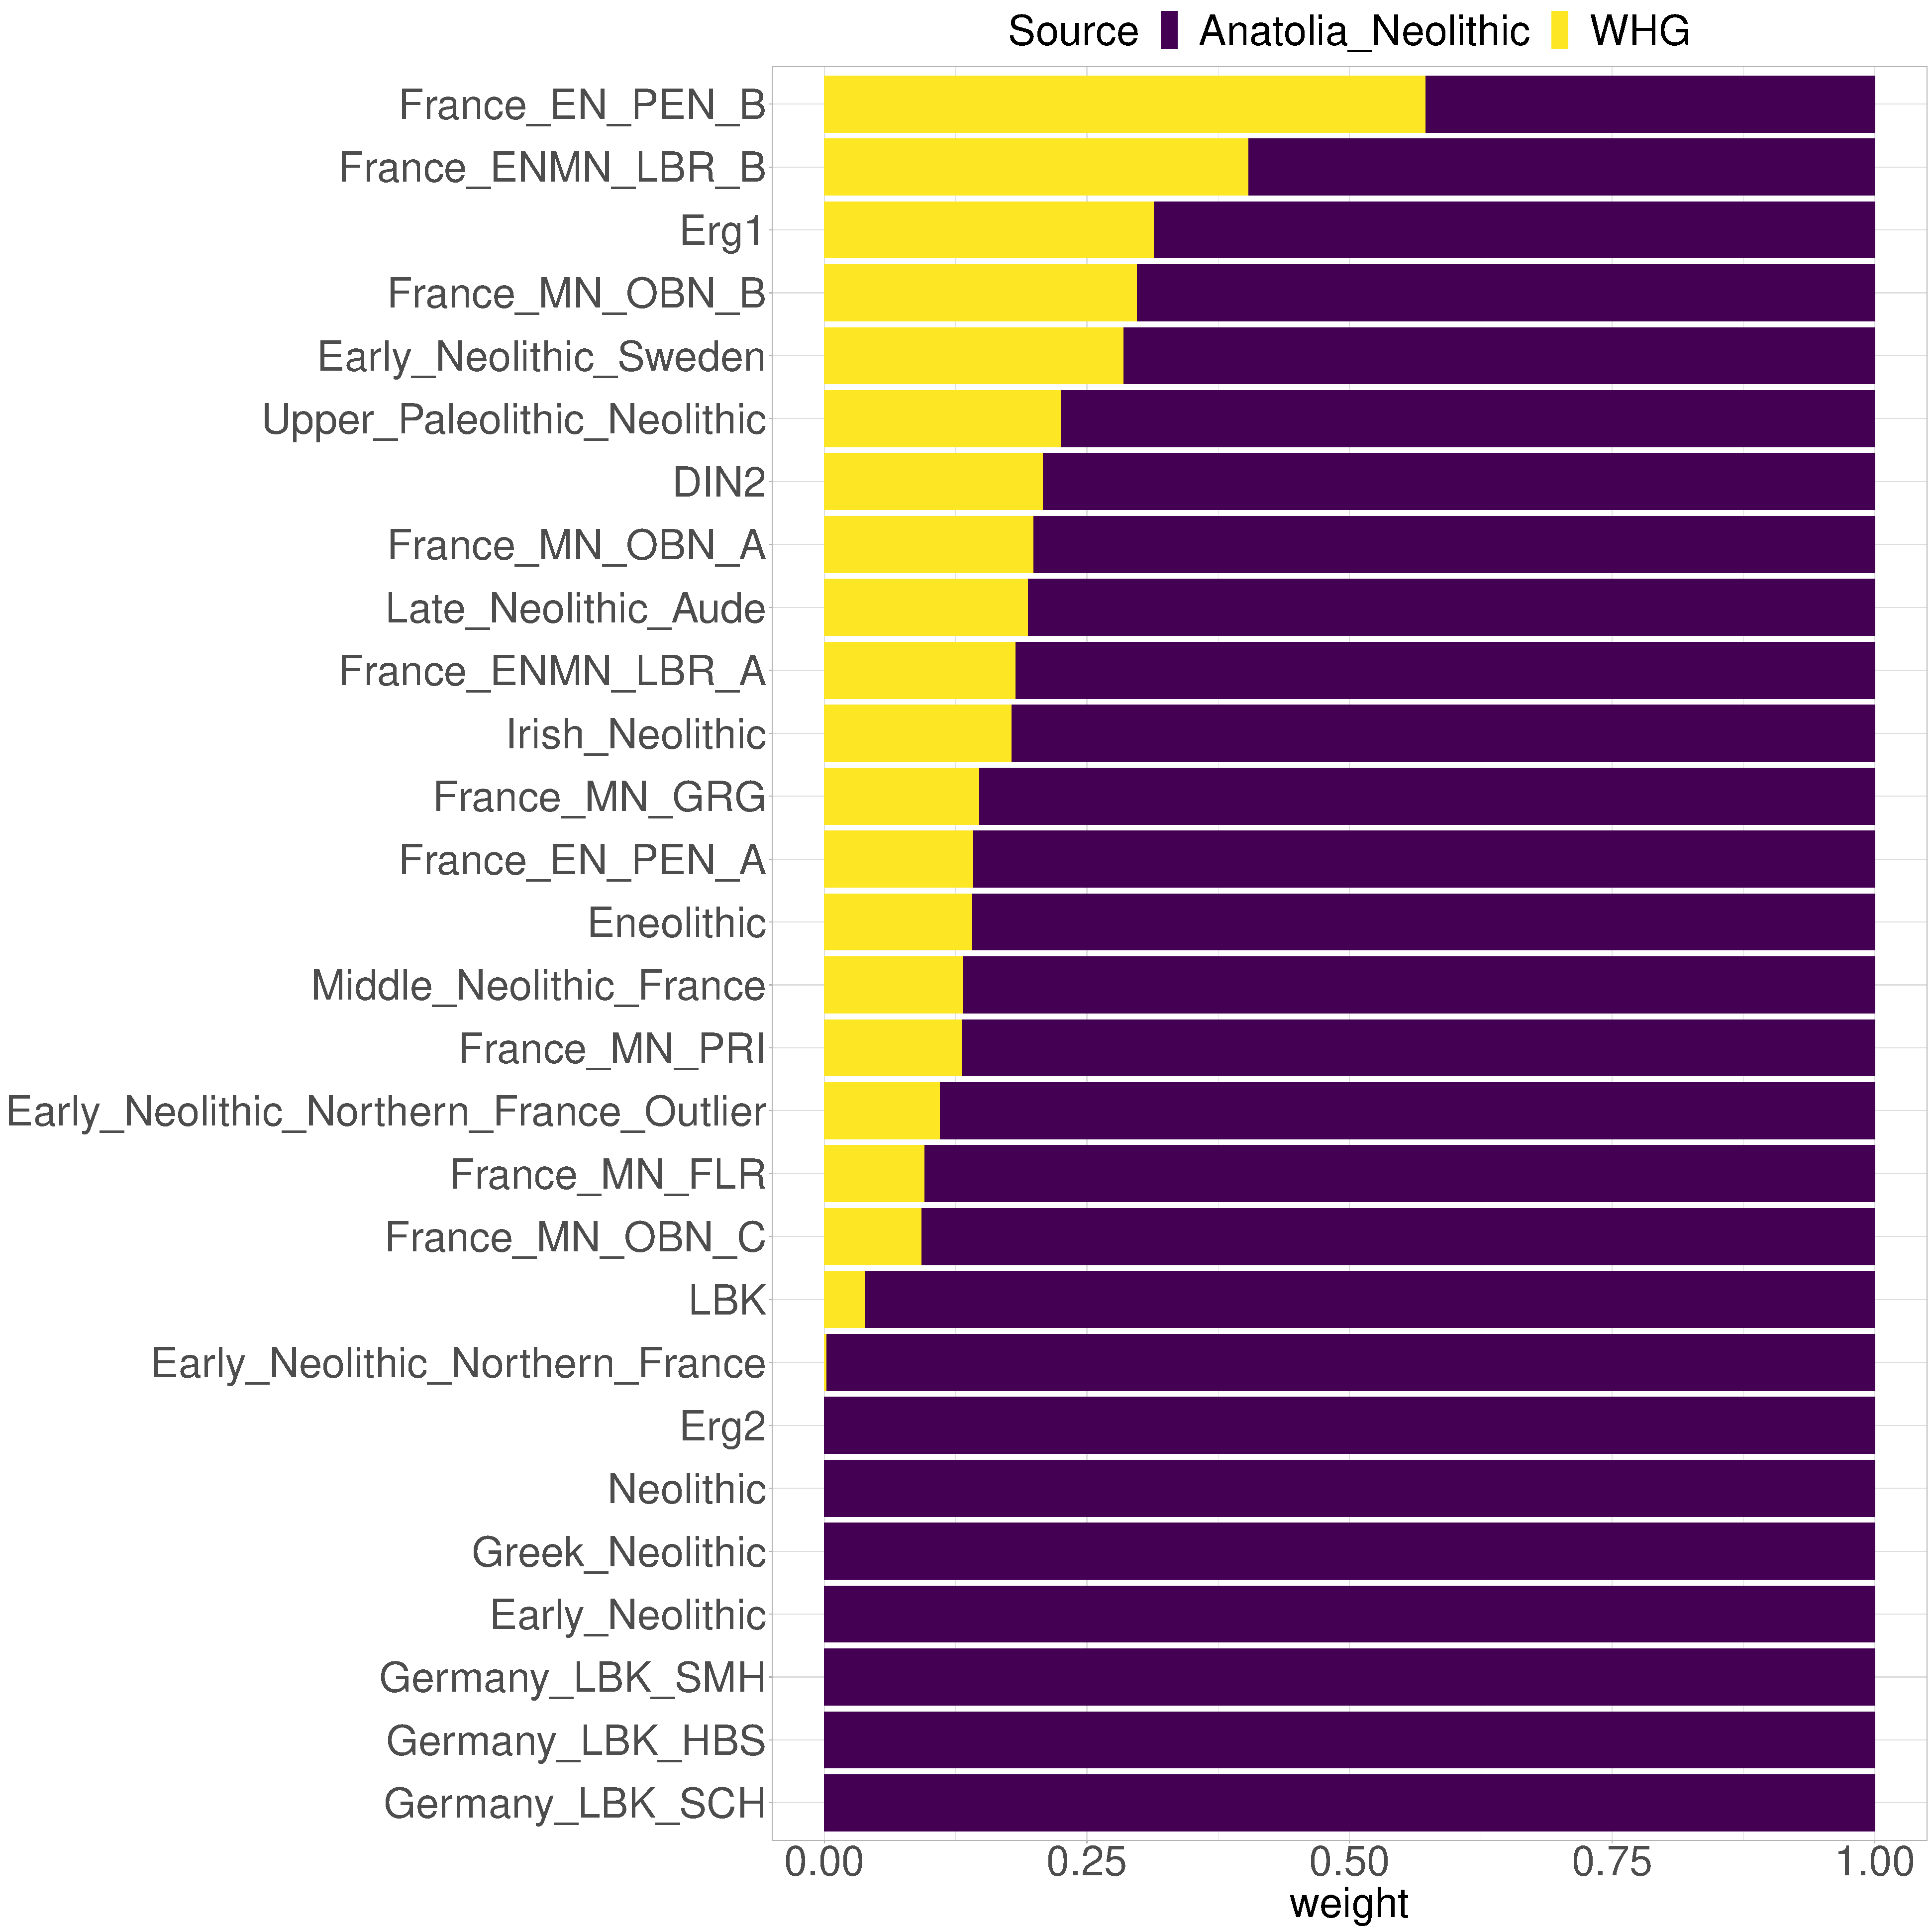
\includegraphics[width=1.0\textwidth]{../images/chapter4/HG_ancestry_Neolithic.pdf}
    \caption{qpAdm ancestry proportion estimates for a selection of European Neolithic individuals. All individuals were modeled as a 2-way mixture between Anatolian Neolithic farmers and Western-Hunter Gatherers (WHG). Outgroups used are \textit{Mota}, \textit{Kostenki14}, \textit{papuan}, \textit{han}, \textit{hannchina}, \textit{mbutipygmy}, \textit{sannamibia}, \textit{yakut}}
    \label{fig:HG_ancestry_Neolithic}
\end{figure}


\begin{figure}[htp]
    \centering
    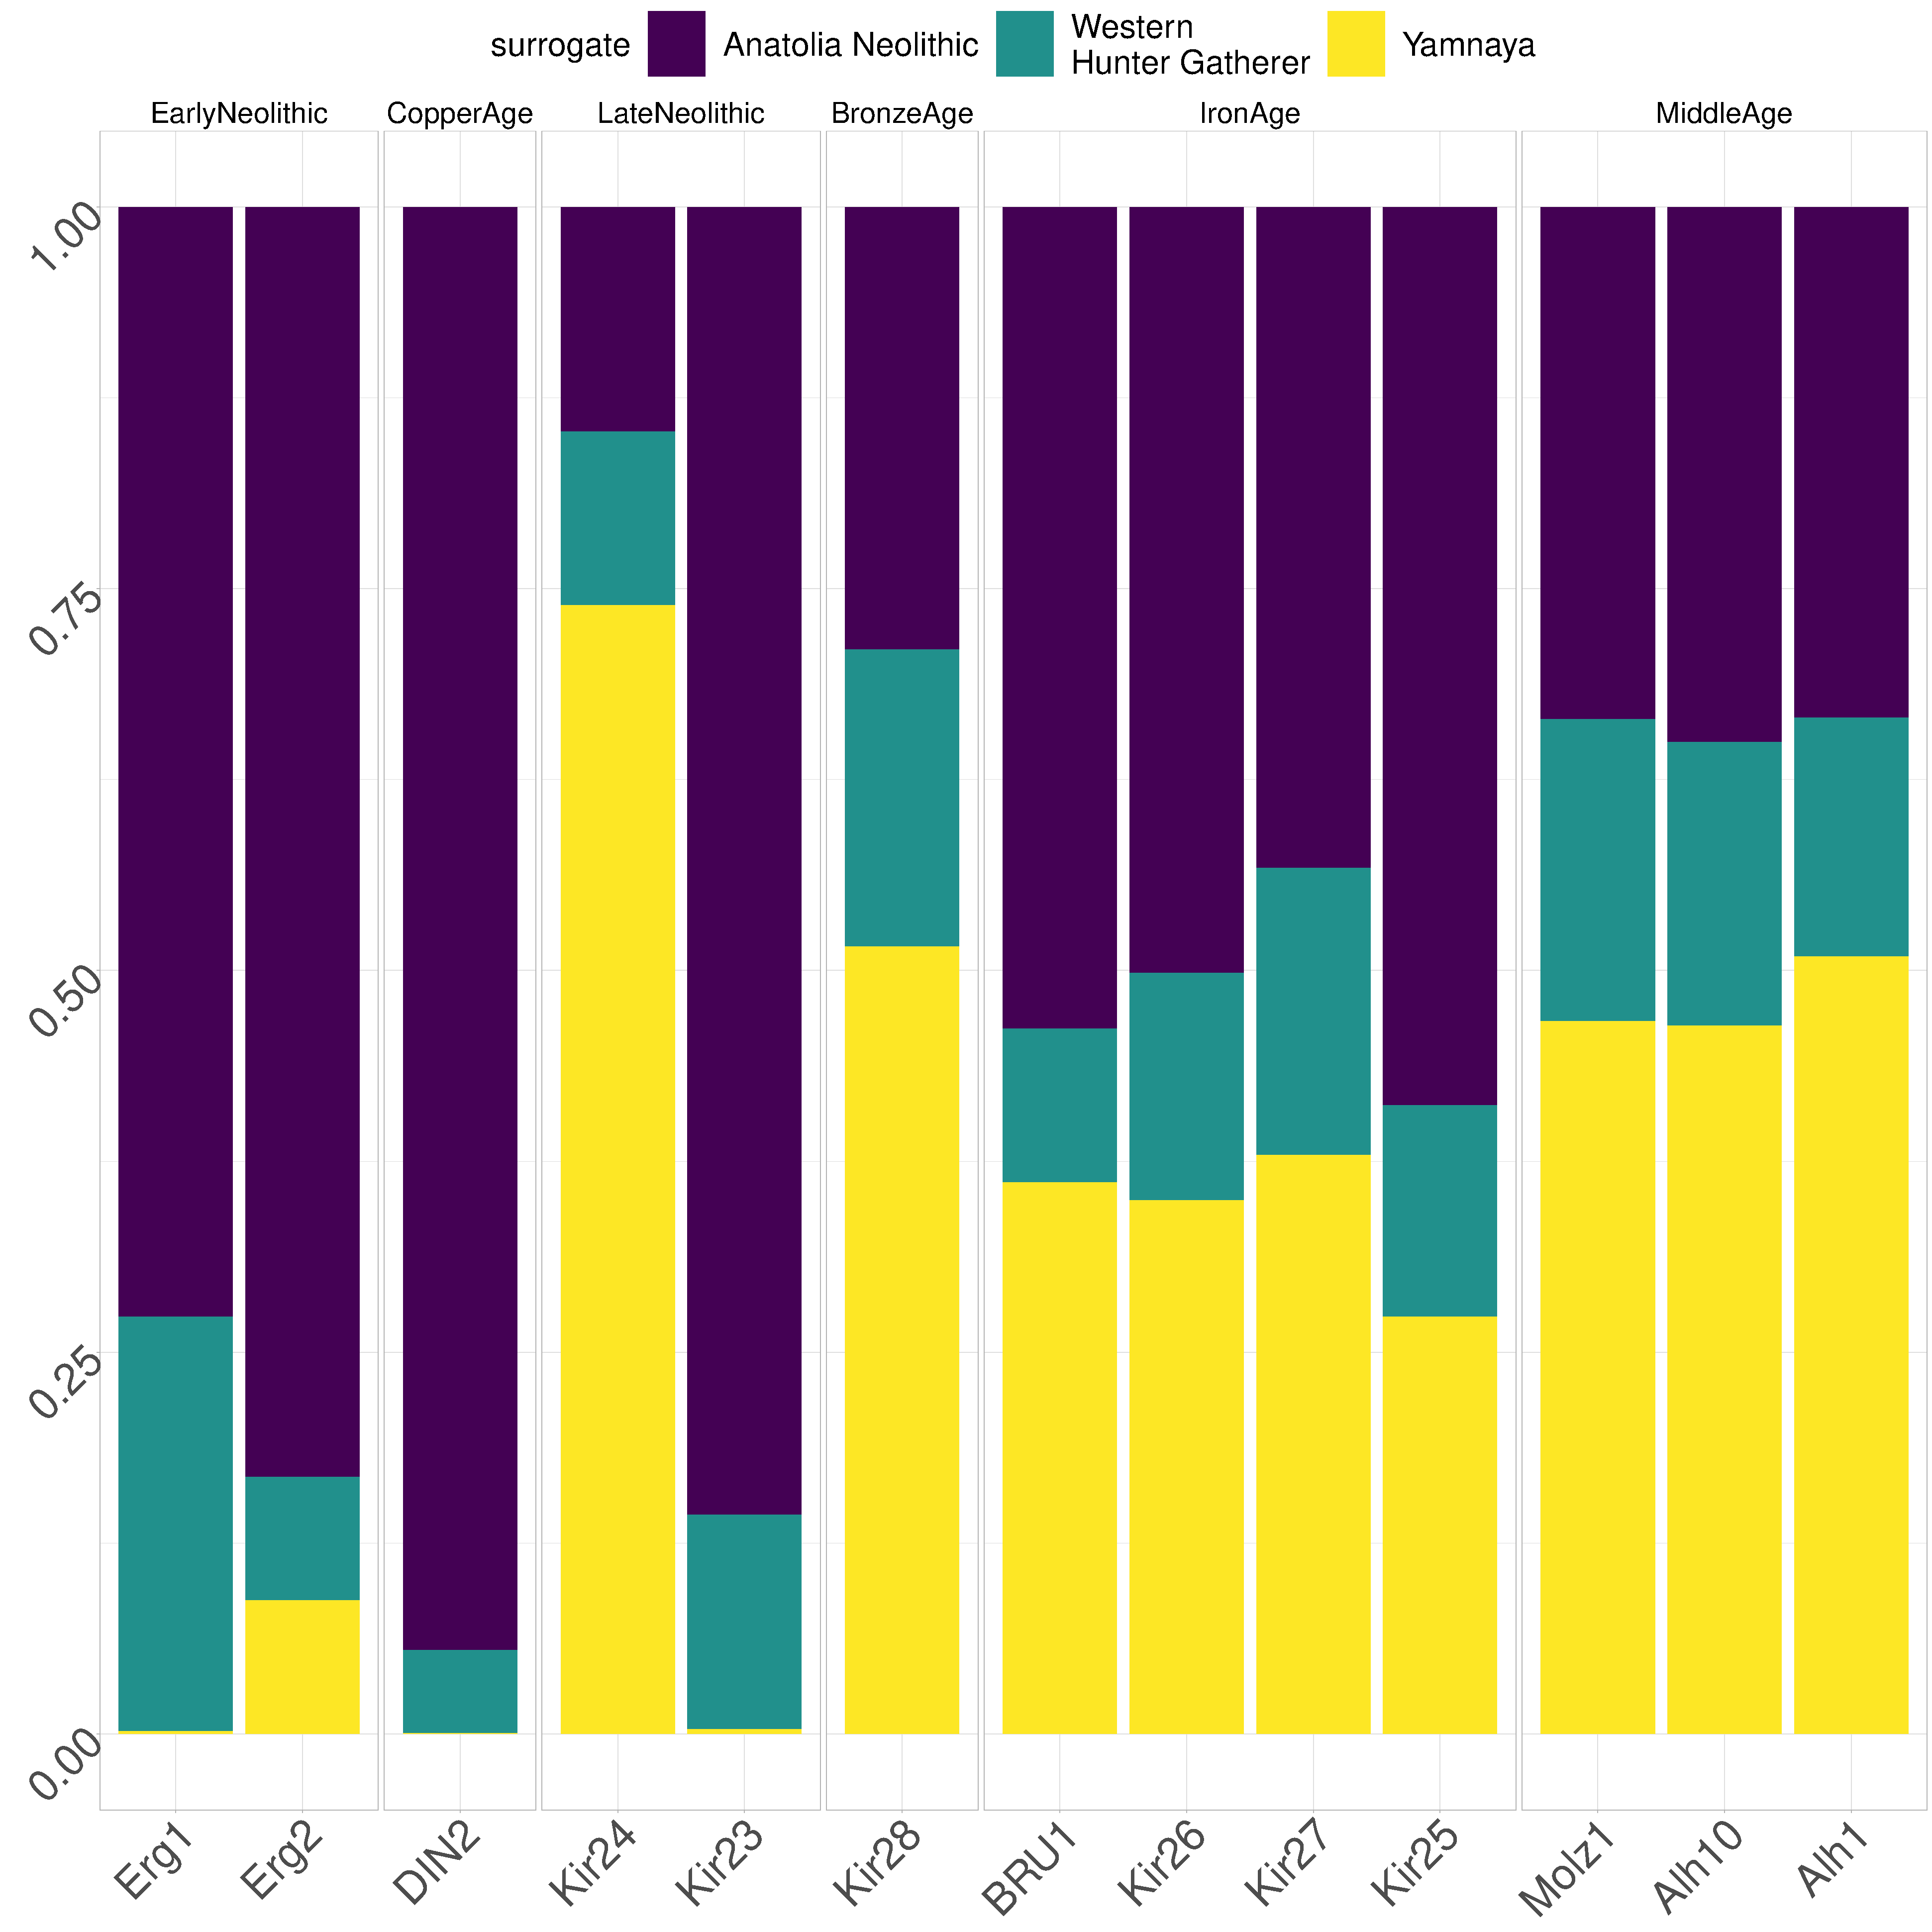
\includegraphics[width=1.0\textwidth]{../images/chapter4/plots3PopBarlot.pdf}
    \caption{SOURCEFIND ancestry proportion estimates for all newly sequenced target samples (vertical columns). Target samples are grouped by archaeological age. Surrogate populations are represented as horizontal rows and also grouped into archaeological culture. Each target was modeled as a mixture of only populations which are dated to being older or contemporaneous as the the target. Numbers within each cell correspond to the ancestry proportion estimate.}
    \label{fig:plots3PopBarlot}
\end{figure}

\subsection{Spatially and temporally close samples in Late Neolithic display highly distinct ancestries}

This dataset included two individuals found in the same stratigraphical layer of Cherry-Tree cave; Kir23 and Kir24 were both dated to the Late Neolithic (approx 4700 BP). Despite their temporal and spatial closeness, they show highly different ancestry profiles (Fig. \ref{fig:plots3PopBarlot}). 

On both the plink PCA and fineSTRUCTURE clustering, Kir24 clusters with individuals from populations present around the Eurasian Steppe during the Bronze-Age, such as those from the Yamnaya and Afanasievo cultures. These are the populations thought to be in part responsible for the spread of Indo-European languages across Europe \cite{Haak2015}.  That the Yamnaya and Afanasievo samples were sampled in Russia suggests that Kir24 may have been a recent migrant from the Eurasian Steppe. This is supported by IBD analysis; of all the ancient samples in the dataset Kir24 shares the most IBD (31.12cM) with the Yamnaya type-specimen and the lowest $TVD$ with 2 other members of the Yamnaya population. This timing (Kir24 is dated to approximately 4700 BP) corresponds to some of the earliest appearance of Yamnaya-like ancestry in central Europe \cite{Racimo8989}. Using qpAdm, Kir24 could be modelled as a mixture of Yamnaya (93\%, se=12) and WHG (6\%, se=8) without any Neolithic ancestry. 

Kir24 was assigned to mtDNA haplogroup T1a1, which has been found in Yamnaya samples from the Middle Volga region and Bulgaria \cite{keyser2009ancient}; the same study found the frequency of T1a1 to be higher in the Yamnaya peoples than in any other ancient or modern population. 

On the other hand, Kir23 is found in a fineSTRUCTURE cluster with Ballynahatty, from Neolithic Ireland (3343-3020 BC), and is positioned on both plink and ChromoPainter PCAs with other late Neolithic samples. It is found in adjacent fineSTRUCTURE groups to samples from Neolithic Spain and Ireland. As is the case with other Neolithic samples of this era, Kir23 has a component of Hunter-Gatherer ancestry; it is known that Middle Neolithic individuals are characterised by admixture with the existing Hunter-Gatherer populations. qpAdm modelling showed that Kir23 could be formed from a mixture of Neolithic Anatolia (96\%, se=14)  and Hunter Gatherer (6.25, se=0.91) without the need for additional Steppe ancestry. 

To test whether the source of Neolithic ancestry in Kir23 was most similar to local populations, I performed $f_{4}$ tests in the form $f_{4}(W=Kir23, X=mbutipygy; Y=test, Z=Erg2)$, which tests whether Kir23 forms a clade with Erg2, a local farmer individual, or $test$, where $test$ was one of several different farmer populations. Erg2 was chosen as the local group because it did not infer any potentially confounding Hunter Gather ancestry. Kir23 always formed a clade with Erg2, suggesting that the source of ancestry into Kir23 was local and that there was a degree of continuity within the region. 


\subsection{`Southern' ancestry to Cherry-Tree Cave during the Iron Age is Italian in origin}

The plink PCA shows that the four Iron Age samples are shifted towards the cluster of Neolithic individuals and away from the samples typical of the European Bronze Age. The same pattern is also seen in the present-day PCA, where the Iron Age samples are shifted substantially towards Spain / Northern Italy relative to the preceding Bronze Age sample which is situated among Northern / Western European populations (Germany, Wales) (Fig. \ref{fig:chunklengths_moderns_ancients_PCA_bav}). 

In fineSTRUCTURE, all four Iron Age individuals were grouped alongside several Lombard samples and a Roman soldier from 300AD. qpAdm modelling showed that the Iron Age samples can be well formed from a mixture of the preceding Bavarian Bronze age sample and those from either Renaissance Italy, Imperial Rome, Imperial Rome Late Antiquity or `Roman Solider' from Veeramah et al (2018), with all other possible sources included with Bronze Age giving a poorly fitting models (Table \ref{tab:IronAge_qpAdm}). This suggests a model of admixture from populations best represented by those from post Iron-Age Italy. SOURCEFIND using all ancients as surrogates, inferred 26\% of the IA samples' ancestry was most closely related to the ``Rennaisance'' Italy population from 1500CE, with no such inferred ancestry in the temporally flanking Bronze and Middle Age samples.

\begin{table}
\centering
\begin{tabular}[t]{llrrr}
\toprule
Target & Left & Weight & SE & Z\\
\midrule
Bavaria Iron & Bavaria Bronze & 1.458 & 0.732 & 1.992\\
Bavaria Iron & HallstattBylany & -0.458 & 0.732 & -0.625\\
\addlinespace
Bavaria Iron & Bavaria Bronze & 0.956 & 0.426 & 2.245\\
Bavaria Iron & Renaissance & 0.044 & 0.426 & 0.103\\
\addlinespace
Bavaria Iron & Bavaria Bronze & 0.986 & 0.202 & 4.871\\
Bavaria Iron & Imperial Rome Late Antiquity & 0.014 & 0.202 & 0.070\\
\addlinespace
Bavaria Iron & Bavaria Bronze & 0.990 & 0.173 & 5.738\\
Bavaria Iron & Imperial Rome & 0.010 & 0.173 & 0.056\\
\addlinespace
Bavaria Iron & Bavaria Bronze & 0.981 & 0.280 & 3.505\\
Bavaria Iron & Roman Solider & 0.019 & 0.280 & 0.069\\
\bottomrule
\end{tabular}
\caption{Selected qpAdm results for estimating proportions of ancestry in the four Bavarian Iron Age samples. Each two rows is one test, with left populations as Bavaria Bronze and other. `Weight' gives proportion of ancestry, `SE' jackknifed standard error of Weight. Note negative Weight for model involving  HallstattBylany, showing that the model does not fit well}
\label{tab:IronAge_qpAdm}
\end{table}


MOSAIC inferred the Iron Age samples could be formed of a mixture of $\approx$ 18\% ancestry from a source closest to an Alamannic-Frankish sample (STR\_355c, 510 – 530 AD) and $\approx$82\% ancestry from a source closest to Anatolian Neolithic / LBK samples, with admixture dated to 9.2 generations ago (bootstrapped 95\% CI: 7.86-11.31). $F_{st}$, estimated by MOSAIC, between the two mixing sources was 0.016, approximately equivalent between present-day Germans and Palestinians \cite{nelis2009genetic}.  


Based on SOURCEFIND and qpAdm modelling with selected ancient and present-day East Asian samples, unlike Gamba et al (2014) \cite{Gamba2014}, I found no evidence of East-Asian or East-Asian-like admixture (Fig. \ref{fig:chapter4resultsSFheatmapolder}).


\subsection{Present-day genomes unpick genetic differences between early Germanic and Slavic populations}

Lastly, my dataset included three samples (1 newly sequenced) from the Middle Age period. The two genomes from Altheim, Germany, date to around 500AD and were found in a Roman context. The single individual from Molzbichl, Austria, dates to around 300 years later, and has been assigned to a `Slavic' cultural context. It is currently unknown whether, in addition to cultural and linguistic differences, genetic differentiation exists between the `Germanic’ peoples represented by the two Altheim samples, and the `Slavic’ peoples represented by the Molzbichl sample.

The three Middle Age samples appear to share common ancestry based on the plink PCA and are located next to other spatially and temporally close samples from the Middle Ages. Similarly, they have almost indistinguishable SOURCEFIND ancestry proportions (Fig \ref{fig:plots3PopBarlot}).

$f_{4}$ in the form $f_{4}(mbutipygymy, Bavaria\_Iron; Bavaria\_Slav, Bavaria\_Germanic)$ returned a non-significant result, consistent with `Germanic' and `Slavic' populations splitting post Iron Age. However this non-significant result could be caused by low sample sizes in the Middle Age populations or a lack of power in allele-frequency based methods.

However, the two Germanic samples fall into a fineSTRUCTURE cluster with a set of contemporaneous samples from Northern Europe, including 10-11\textsuperscript{th} century Vikings from Estonia, Sweden and Iceland \footnote{Viking samples not shown on Fig. \ref{fig:plink_PCA} to increase visual clarity} , whereas Molz1 clusters with other individuals known to be from Early Slavic populations. Interestingly, the Slavic cluster also containing a sample DA29, also know as `GoldenHordeEuro'. This sample is from Karasuyr, Kazakhstan, and has dated to 1200-1400 CE. The Golden Horde was a Mongol khanate established in the 13th Century CE. Given this sample shows clear evidence of European ancestry and clusters alongside individuals from Early Middle Age Europe, it has been proposed that this individual was captured in Europe during the Mongol raids of the 13th Century, when they assaulted the Kievan Rus' federation \cite{de2018137}. That `GoldenHordeEuro' clusters with Molz1 suggests the location of capture in Europe may have been from Austria where Molz1 was found.

On a haplotype-based PCA with modern samples, Molz1 clusters with present-day Slavic speaking populations such as Poland, Ukraine and Belarus, while the two Germanic samples cluster with present-day individuals from Germanic-speaking countries in Western Europe, such as Scotland, Germany and Wales (Fig. \ref{fig:chunklengths_moderns_ancients_PCA_bav}). Plotting differential haplotype sharing between the Slavic and Germanic sample makes this pattern clear (Fig \ref{fig:germanic_slavic_HB_sharing}). There is a clear division down the centre of Europe, dividing it into East and West that shows the structure in present-day Europeans has existed since at least the Early Middle Ages. 

In SOURCEFIND, the two samples from Altheim derived a large proportion of their ancestry to modern day Germans (81.8\%, se=12.8), whereas the Molzbichl sample derived a large proportion of its ancestry from modern day Polish (77.85\%, se=20.3) and Croatians (11.7\%, se=9.1). 

\begin{figure}[htp]
    \centering
    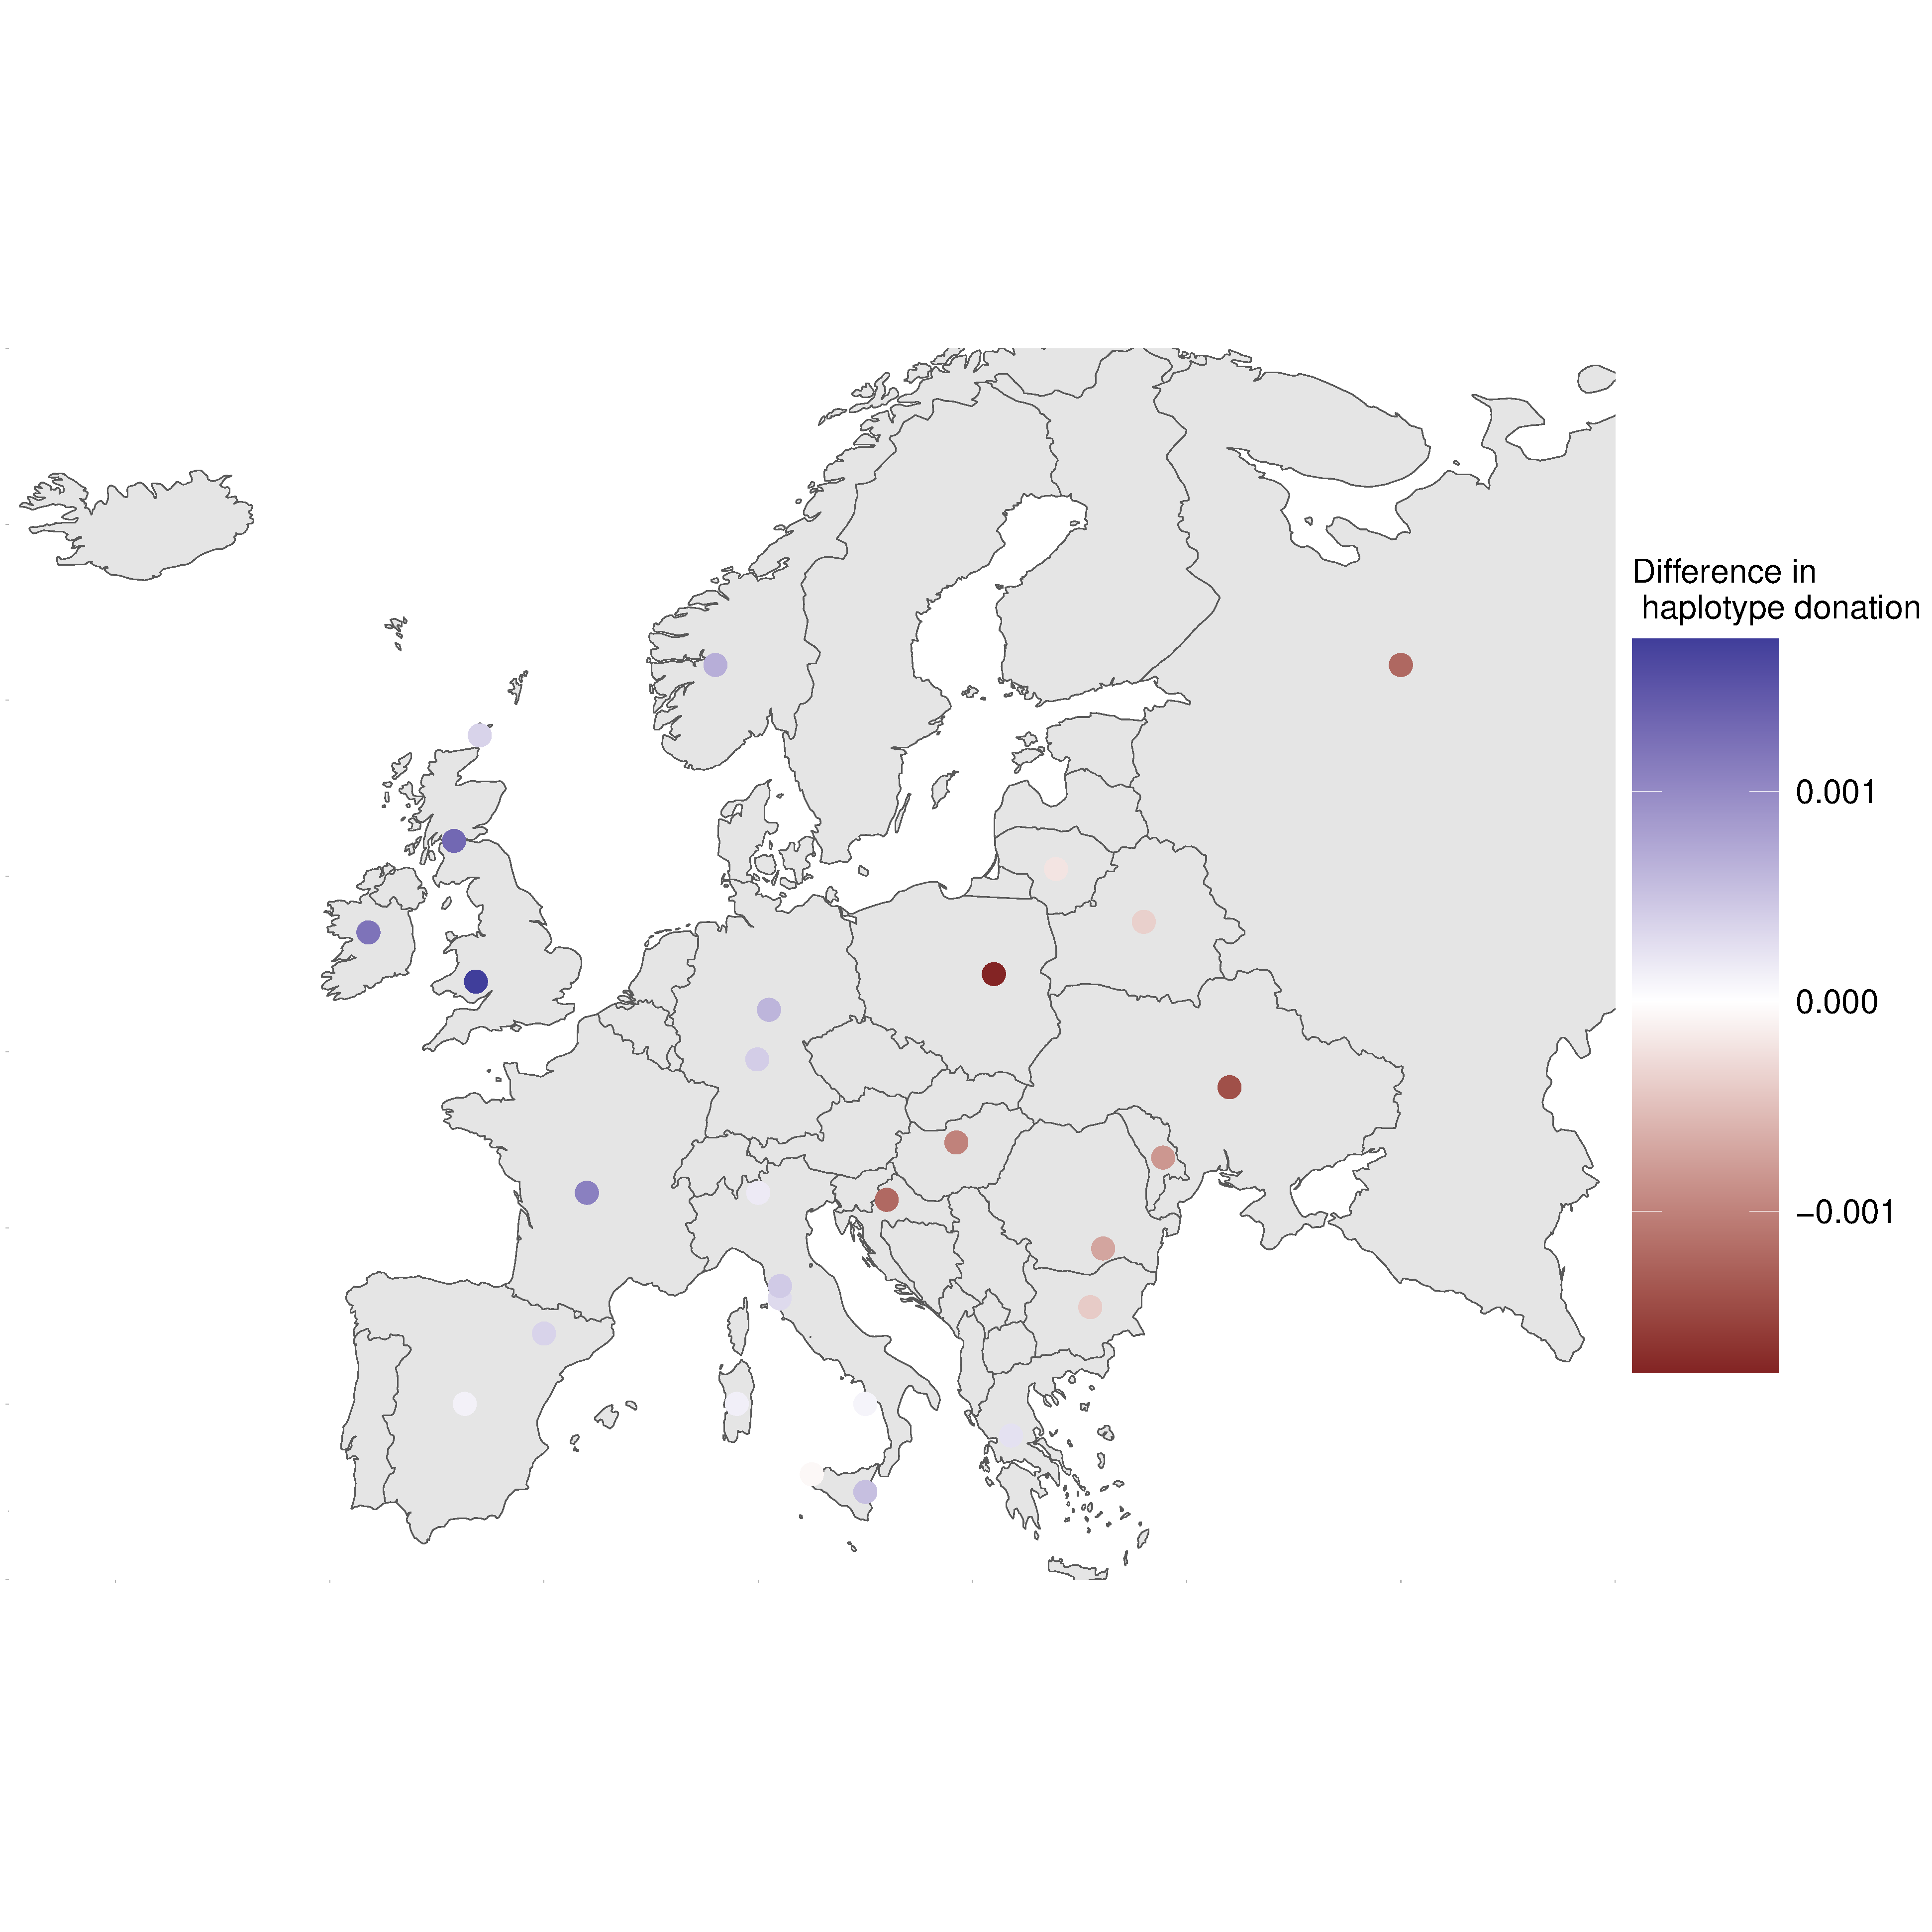
\includegraphics[width=1.0\textwidth]{../images/chapter4/germanic_slavic_HB_sharing.pdf}
    \caption{Differential haplotype-donation between Germanic and Slavic samples. Each coloured point is one present-day population. Points are coloured based on whether they donate relatively more to Germanic (blue) or Slavic (red) ancient samples.}
    \label{fig:germanic_slavic_HB_sharing}
\end{figure}

\subsection{Summary of Results and Discussion}

Drawing back to the questions asked at the beginning.

Whilst the two samples from the Early and Middle Neolithic, Erg1 and DIN2, showed some signs of being from at least closely related source populations, they also displayed variation suggestive of different population histories. Consistent with the hypothesis that DIN2 may have migrated along the Danubian route, it shares the lowest $TVD$ and is found in a fineSTRUCTURE cluster with other samples from the Hungarian Plane. Most importantly, Erg1 and DIN2 two samples also showed differences in the degree of Hunter-Gatherer ancestry; whilst DIN2 showed no evidence of admixture, Erg1 likely had a recent Hunter-Gatherer ancestor.

I found evidence of population discontinuity in Cherry-Tree Cave from the Late Neolithic through to Iron Age. I identified a incoming signal of `southern' ancestry during the Iron Age, which was not present in the single sample from the preceding Bronze Age. The most plausible source of this ancestry is from Italy, with the best source in the dataset being the cluster of Renaissance samples from Antonio et al (2019) \cite{antonio2019ancient}, date to between 282 - 354 AD. This, combined with evidence the Iron Age samples cluster with present-day individuals from north Italy and historical evidence of Lombard migrations to Southern Germany \cite{wegewitz1972}, suggests they may be the admixing source. Whilst collaborators proposed that the source may be related to the local Hallstatt culture, qpAdm modelling rejected this scenario (Table \ref{tab:IronAge_qpAdm}). Wherever the source originated from, this admixture event provides strong evidence against continuity in Cherry-Tree Cave. 

Lastly, I used present-day genomes of individuals from across Europe to show that there are clear genetic differences between the Middle Age Germanic and Slavic samples, with the Germanic samples showing a strong affinity to western European countries and the Slavic samples showing a strong affinity to eastern European samples (Fig. \ref{fig:germanic_slavic_HB_sharing}). However, in the context of ancient samples, all three Middle Age samples clustered with local samples from the Bronze Age rather than the Iron Age (Fig. \ref{fig:plink_PCA}). 

This dataset revealed that temporally and spatially close samples may have very distinct genetic ancestry profiles, with Early Bronze Age samples Kir24 and Kir23 showing high levels of Steppe-related and Neolithic ancestry respectively. In particular, Kir24 seemed to be very recently related to the Yamnaya type-specimen sample, sharing 31cM of IBD with it. The arrival of Yamnaya-like ancestry from this early period (2762BC) represents one of the earliest known appearances in the literature. 

Future studies in this region should focus on obtaining a higher density of samples, in particular from the Bronze and Iron Ages; the low number of samples from these time periods mean any results should be interpreted with caution. More samples would show whether the introduction of `southern' like ancestry in the Iron Age was a widespread phenomena, or restricted to a smaller geographic region in Southern Germany. Similarly, a wider sampling of Iron Age groups from Germany, Italy and Switzerland may allow for a more accurate identification of this source.

Whilst the utility of using present-day genomes was outlined through the comparison of the Slavic and Germanic samples, the analysis would have been significantly improved with higher resolution data from Germany. The data I have, described in Appendix section \ref{section:MSPOBIHellBus}, only had country-level details. Data which had labels from different sub-regions in Germany, similar to the POBI dataset, would have allowed for a finer-scale investigation into the current east-west genetic divide in present-day Germany.    


\chapter{The genomics of the Slavic migration period, Early Middle Ages and their links to the present day}
\label{chapterlabel5}

\section{Introduction}

The Slavic peoples originated as a diverse network of tribal societies who lived in Central and Eastern Europe from the first Millennia AD \cite{barford2001early} and whose origin, although disputed, is thought to be Polesia (a marshy forested area straddling Poland, Belarus, Russia and Ukraine) \cite{fouracre1995new}. Although various Roman and Greek sources refer to Slavs as \textit{Veneti} and \textit{Spori} as early as the 1st and 2nd centuries AD, the term `Slavs' was first used in writing by Roman bureaucrat Jordanes at the beginning of the 6th century after their attack on the Byzantine empire \cite{curta2006southeastern}. This era, known by historians as The Migration Period, was a period of European history, roughly between 375-568 AD after the fall of the Roman Empire \cite{halsall2007barbarian}, characterised by the large-scale movement of various peoples. The Migration Period began with the Huns moving into Eastern Europe at the end of the 4th Century, occupying an area including present-day Hungary and Romania. During the 5th century, various Germanic groups invaded and established a homeland across parts of the Western Roman Empire. This was followed by the expansion of Slavic populations into regions of low population density in the sixth century.

Across the next two centuries, these peoples had settled across large parts of Europe (Fig. \ref{fig:Slavic_tribes}). In particular, the Early Slavs had expanded southwards into the Balkans and Alps \cite{barford2001early, brather2008archaologie, geary2003myth,gojda1991ancient}. It has been proposed that these migrations were key to forming the foundations of present-day Slavic (speaking) nations \cite{barford2001early}.  

By the beginning of the 12th century, Slavs constituted a large part of a number of many medieval Christian states across Europe. As from this time period, Slavs could be broadly split up in three groups: the eastern Slavs as part of the Kievan Rus', southern Slavs in the Bulgarian Empire, the Principality of Serbia, Kingdom of Croatia and the Banate of Bosnia, and western Slavs in the Principality of Nitra, Great Moravia, the duchy of Bohemia and the Kingdom and Poland. In addition, Slavic settlement also occurred in the Eastern Alps; Slovenia, large parts of present-day Austria and Friul. 

\begin{figure}[htp]
    \centering
    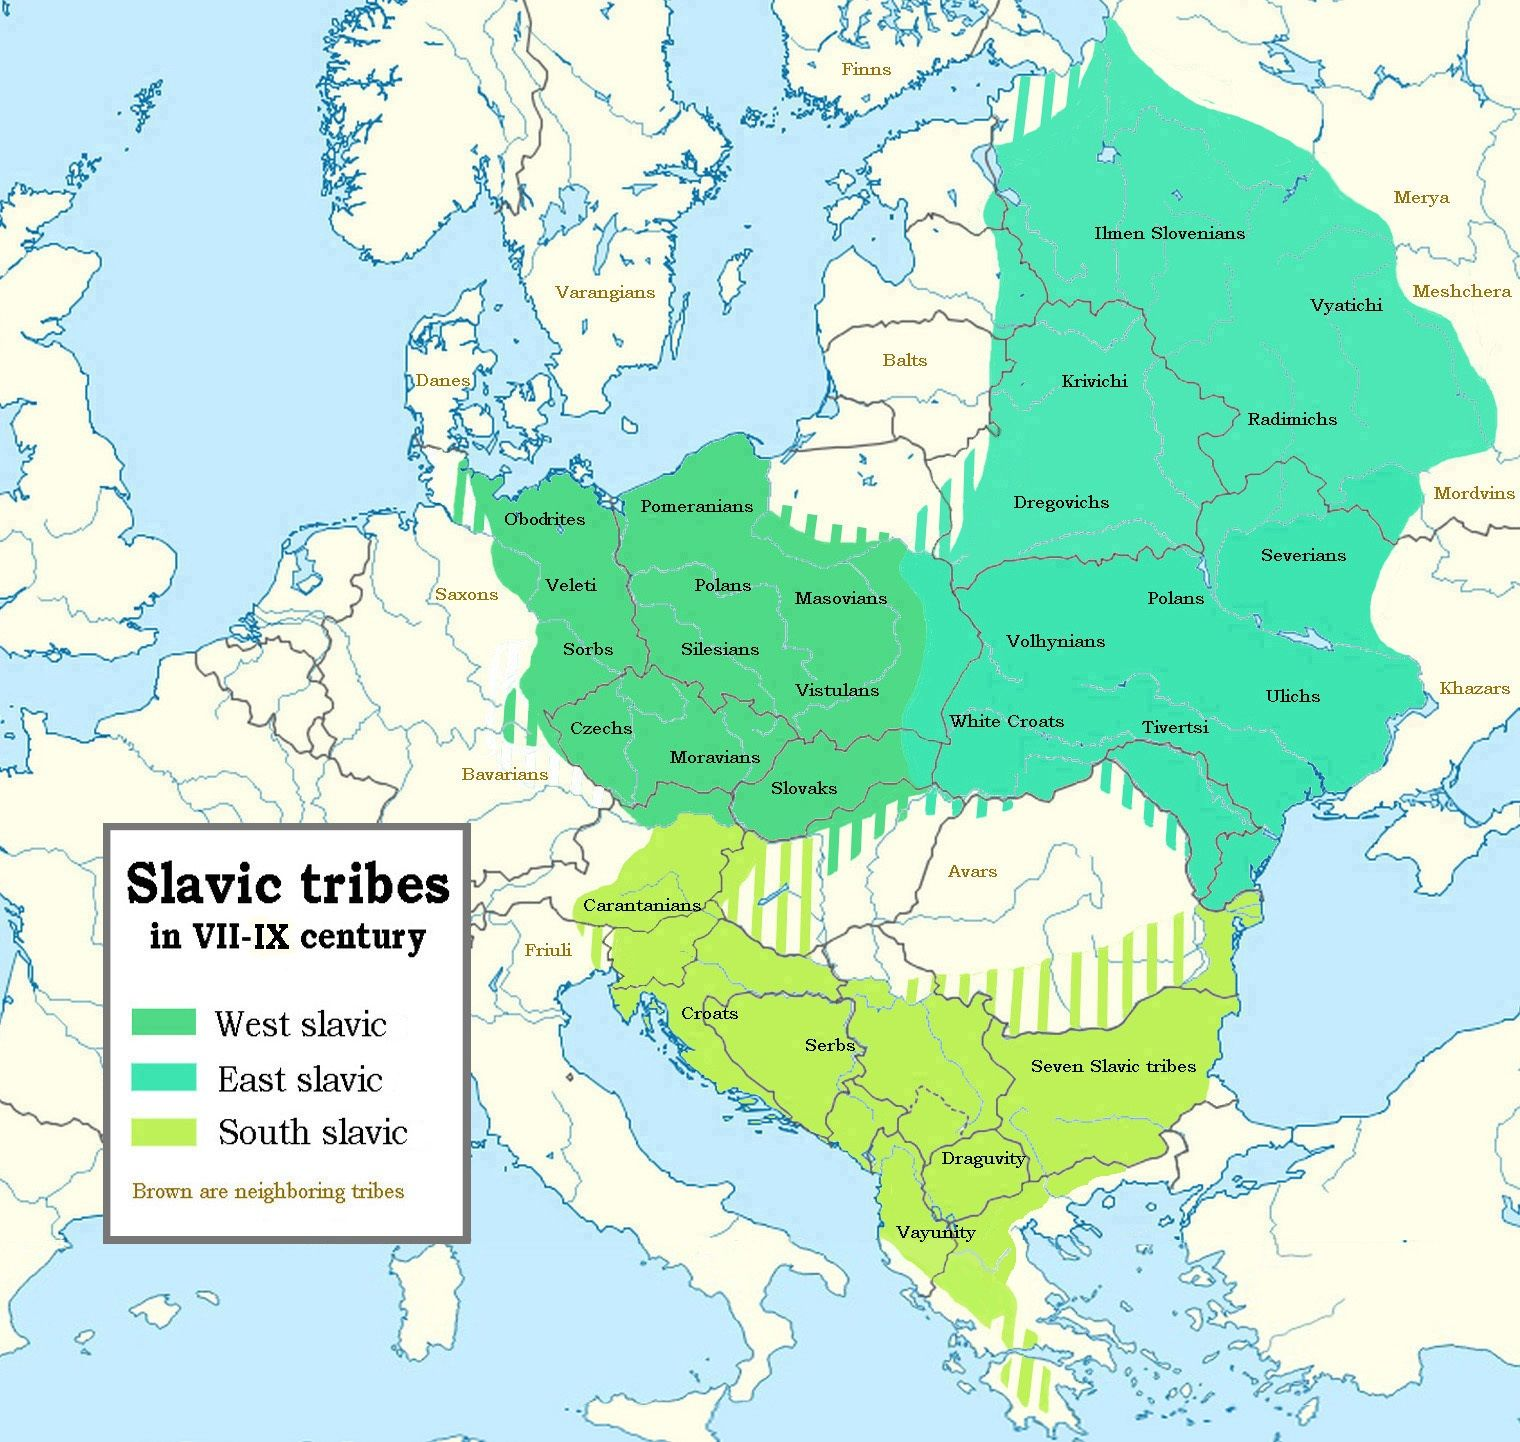
\includegraphics[width=1.0\textwidth]{../images/chapter5/Slavic_tribes_in_the_7th_to_9th_century.jpg}
    \caption{Slavic tribes from the 7th to 9th centuries AD in Europe. Source: (\url{https://commons.wikimedia.org/wiki/File:Slavic_tribes_in_the_7th_to_9th_century.jpg})}
    \label{fig:Slavic_tribes}
\end{figure}

 Today 315 million people speak Slavic languages and linguistic evidence suggests that they can be broadly split into these three broad groups; western Slavs (Poles, Czechs and Slovaks), eastern Slavs (Ukrainians, Belarusians and Russians) and southern Slavs (Croatians, Bulgarians, Slovenians, Bosnians, Macedonians, Montenegrins and Serbians) \cite{sussex2006slavic}. 

The history of the Slavic peoples can be artificially be split into three periods: Migration Period ($\sim$375AD - $\sim$568AD), Early Middle Ages/High Middle Ages ($\sim$600AD - $\sim$1250AD) and present-day. Several previous studies have investigated the genetics of the transitions between these periods. Juras et al (2014) used uni-parental mtDNA markers from ancient DNA samples from Poland to show continuity between both Roman Iron Age period (200 BC – 500 AD) and Medieval Age (1000–1400AD) with present-day Poles, Czechs and Slovaks \cite{Juras2014}. However, whilst informative about sex-biased migrations, uniparental markers carry only a fraction of the information that autosomal markers do, and therefore may provide misleading or incomplete information about the relationship between  samples \cite{Shaw16122, malinsky2018whole}, especially when admixture is prevalent (although see \cite{Mitochondrial}). For example, it is know that mtDNA and nuclear DNA may have different evolutionary histories and thus display discordant phylogenetic trees \cite{posth2017deeply}. 

Kushniarevich et al (2015) \cite{Kushniarevich23015} combined results from mtDNA, non-recombining Y and autosomal DNA to investigate the population structure of a wide range of present-day Balto-Slavic populations. They proposed that incoming Slavic speakers admixed with peoples in the regions they occupied during the Migration Period. 

More recently, Macháček et al (2021) \cite{MACHACEK2021105333} analysed a cattle rib from Lány, Czechia, dated to approximately 600AD, that is inscribed with Germanic runes. The bone was found in a location where Slavs were thought to have arrived at the end of the Migration Period, after the Germanic tribes had disappeared and the use of a Slavic language is historically confirmed as of the 9th century. However, whether there was early genetic contact as well is yet to be determined. 

Several studies into present-day Slavic populations have detected signatures of admixture from East-Asia \cite{Hellenthal2014, pankratov2016east, MOSAIC_2019, maliarchuk2008origin, qin2015quantitating}. Whether or not these signals can be observed in ancient individuals is yet to be seen and could further refine the admixture date. For example, different admixture dates in different Slavic populations may reveal structure among present-day Slavs. 

Finally, several studies have used haplotype-based methods to explore the structure of present-day Slavic populations. Ralph and Coop \cite{RalphCoop2013} compared regions of IBD matching  across different European populations. They found a relatively high degree of IBD sharing among pairs of individuals from Eastern Europe, suggestive of expansion from a smaller, common source population. This expansion was tentatively estimated to between 0-1000AD. Consistent with estimates of a small population size, Hellenthal et al (2014) \cite{Hellenthal2014} inferred an excess of among Eastern European individuals and an admixture event, albeit with a more constrained admixture date of 440 - 1080 CE. However, this could also be interpreted in terms of a small effective population size \cite{al2019estimating, ringbauer2017inferring}. Salter-Townshend and Myers (2019) also identified admixture in the Chuvash people between east Europeans and east Asians approximately 1224 CE \cite{MOSAIC_2019}.

In this chapter, I will analyse 17 new medium to high coverage whole ancient genomes from Czech Republic, spanning from the Migration Period to Early Middle Ages (384-950 AD). These are, to my knowledge, the first high-coverage whole ancient-genomes from this period. I will merge the newly sequenced samples with reference data from other ancient individuals and a large reference set of relevant present-day European individuals in order to understand their ancestry in the context of both present-day and ancient samples. In particular, I am interested in considering the following questions:

\begin{enumerate}
\item Do the labels "Migration Period" and "Early Middle Ages" make sense from a genetic standpoint? Is there evidence of genetic change between Migration period and Early Middle Ages in the area of present-day Czech Republic? 
\item To what degree to we observe evidence of continuity/discontinuity between the Migration Era and Early Middle Age samples?
\item How are present-day Slavic speakers structured, and do the different ancient Slavic samples have different affinities to different present-day Slavic language groups?
\end{enumerate}


\section{Methods}

\subsection{Description of samples}

Whole-genome sequence data were generated from 17 ancient individuals by collaborators at Max Plank institute for E(Table \ref{tab:AncientSamples}). Five samples from Líbivá date to the Migration Period (348 AD - 504 AD), while the other 12 samples from Pohansko date to the later Early Middle Ages (724 AD - 995 AD).

\begin{table}
\centering
\begin{tabular}[t]{llrlr}
\toprule
Code & Site & Date (AD) & Period & Coverage\\
\midrule
LIB11 & Břeclav – Líbivá & 741.5 & Early Middle Ages & 5.3\\
LIB12 & Břeclav – Líbivá & 475.5 & Migration period & 6.8\\
LIB2 & Břeclav – Líbivá & 495.0 & Migration period & 6.4\\
LIB3 & Břeclav – Líbivá & 509.0 & Migration period & 5.3\\
LIB4 & Břeclav – Líbivá & 472.5 & Migration period & 6.5\\
\addlinespace
LIB5 & Břeclav – Líbivá & 348.0 & Migration period & 7.3\\
LIB7 & Břeclav – Líbivá & 830.5 & Early Middle Ages & 5.6\\
POH11 & Pohansko – Lesní školka & 783.0 & Early Middle Ages & 5.0\\
POH13 & Pohansko – Lesní školka & 879.5 & Early Middle Ages & 6.0\\
POH27 & Pohansko – Jizní Předhradí & 783.0 & Early Middle Ages & 5.9\\
\addlinespace
POH28 & Pohansko – Jizní Předhradí & 822.5 & Early Middle Ages & 5.6\\
POH36 & Pohansko – Jizní Předhradí & 880.5 & Early Middle Ages & 5.5\\
POH39 & Pohansko – Jizní Předhradí & 866.4 & Early Middle Ages & 5.3\\
POH3 & Pohansko – Lesní hrúd & 956.5 & Early Middle Ages & 5.4\\
POH40 & Pohansko – Lesní školka & 950.5 & Early Middle Ages & 5.5\\
\addlinespace
POH41 & Pohansko – Lesní školka & 875.5 & Early Middle Ages & 5.2\\
POH44 & Pohansko – Pohřebištĕ U Kostela & NA & Early Middle Ages & 5.3\\
\bottomrule
\end{tabular}
\caption{Information on newly sequenced ancient samples. Date (AD) estimated from radiocarbon dating. `Migration' corresponds to Migration Period and `EMA' corresponds to Early Middle Ages. Coverage calculated as the mean depth across all 77,213,942 genome-wide SNPs where genotypes were called at.}
\label{tab:AncientSamples}
\end{table}

The Migration Period and Early Middle Age samples were categorised based upon the style of pottery found in the burial grounds (Z. Hofmanová, personal communication).  


\subsection{Processing of samples performed by collaborators}

Sequencing quality of reads was checked with fastQC. Duplicate reads were marked with picard-tools MarkDuplicates. Libraries from the same samples were merged using SAMtools merge, and duplicates were marked again as described above to tag duplicate reads of the same libraries among sequencing lanes. Genotypes and genotype likelihoods were called using the atlas pipeline. First, aligned reads from paired-end sequenced read groups were merged to avoid double-use of bases in the overlapping part. PMD patterns were estimated for each read group with ATLAS task=PMD, providing the reference with ref= and enabling the option filterSoftClips to remove reads with soft-clipping. 
Base quality recalibration parameters were obtained (short recal-parameters) from highly conserved regions. A .bam file with corrected recalibration and pmd parameters was created with atlas BAMUpdateQualities, providing PMD and recal-parameters and applying soft-clip filter (pmdFile, withPMD, recal, filterSoftClips).

\subsection{Ancient DNA processing} \label{AncientDNAprocessing}

I merged the 17 newly sequenced individuals with the ancient literature samples given in section \ref{section:AncientReferenceDataset}, resulting in a total of 959 ancient individuals with genotype likelihoods at 77,213,942 genome-wide autosomal SNPs. 

I followed the GLIMPSE \cite{rubinacci2021efficient} imputation and phasing pipeline (\url{https://odelaneau.github.io/GLIMPSE/tutorial_b38.html}) to generate genotype probabilities and phased genotypes for each individual. For the reference panel, I used the 30x 1000 genomes dataset \cite{byrska2021high}, described in Appendix section \ref{section:1000genomes}.  

\subsection{Present-day DNA processing} \label{PresentdayDNAprocessing}

I  merged the newly sequenced and published ancient samples with the MS-POBI-HellBus dataset, described in detail in Appendix section \ref{section:MSPOBIHellBus}, chosen because it contains a high number of relevant samples from central and eastern Europe. I removed samples from Australia, New Zealand and USA.

The present-day and ancient samples were phased separately, as GLIMPSE is designed for sequence-level density of data, and the present-day samples were genotyped on a low-density genotyping array. Therefore, I phased the present-day samples using shapeit4 \cite{delaneau2018integrative} using default parameters and the supplied genetic map. I note that phasing the datasets separately may reduce power to compare ancient and present-day samples. 

The present-day and ancient samples described in section \ref{AncientDNAprocessing} were merged and converted to ChromoPainter format.

\subsection{plink PCA}

I performed a PCA on the pre-imputation genotypes for only the ancient samples using plink2 \cite{chang2015second}. I chose to use plink2 because recent studies have shown it is substantially better at dealing with samples containing variable amounts of missing data than other methods such as smartPCA \cite{AlbrechtsenPCAmissingness}.

I ranked all SNPs by the percentage of missing genotypes and retained only the 500,000 markers with the lowest amount of missingness. I then LD-pruned the resulting SNPs using the settings \texttt{--maf 0.01} and \texttt{--indep-pairwise 50 5 0.2} and performed PCA using plink2 under default settings. 

\subsection{Allele-frequency based tests}

I used Admixtools \cite{Patterson2012}, implemented in Admixr R library \cite{admixrpetr2019} to perform  different F-statistics.

\subsection{ChromoPainter and fineSTRUCTURE analysis}

The merged data described in sections \ref{AncientDNAprocessing} and \ref{PresentdayDNAprocessing} contained a total of 959 ancient and 14,795 present-day samples genotyped at 477,417 autosomal bi-allelic SNPs.

I first selected all ancient samples above 2x coverage and performed an `all-v-all' painting where each haplotype was compared to all other haplotypes in turn, hereafter referred to as `ancient' painting. I chose to remove samples with $<$2x coverage because all new samples analysed here had at least 5x coverage, and my previous work indicated little difference in ChromoPainter results among samples $>$2x coverage (Chapter 2 section \ref{sec:ChromoPainterChap2}). 

I also performed an `all-v-all' painting of the 17 newly sequenced samples and the present-day populations given in table \ref{table:present-day_inds_painting}, hereafter referred to as `present-day painting'.


The fineSTRUCTURE \cite{Lawson2012} clustering and tree building algorithm was applied to the ChromoPainter output for both the `present-day' and `ancient' paintings, in each case using 2,000,000 MCMC iterations after 1,000,000 iterations of ``burn-in''. I then ran the tree-building mode (-m T) with 100,000 additional hill-climbing steps before tree building,

Tree figures, coancestry matrix figures and principle component plots were generated using the fineSTRUCTURE R library \url{(https://people.maths.bris.ac.uk/~madjl/finestructure/FinestructureRcode.zip)}.

The full workflow is shown in schematic form in Figure \ref{fig:workflow_slav}.

\begin{figure}[htp]
    \centering
    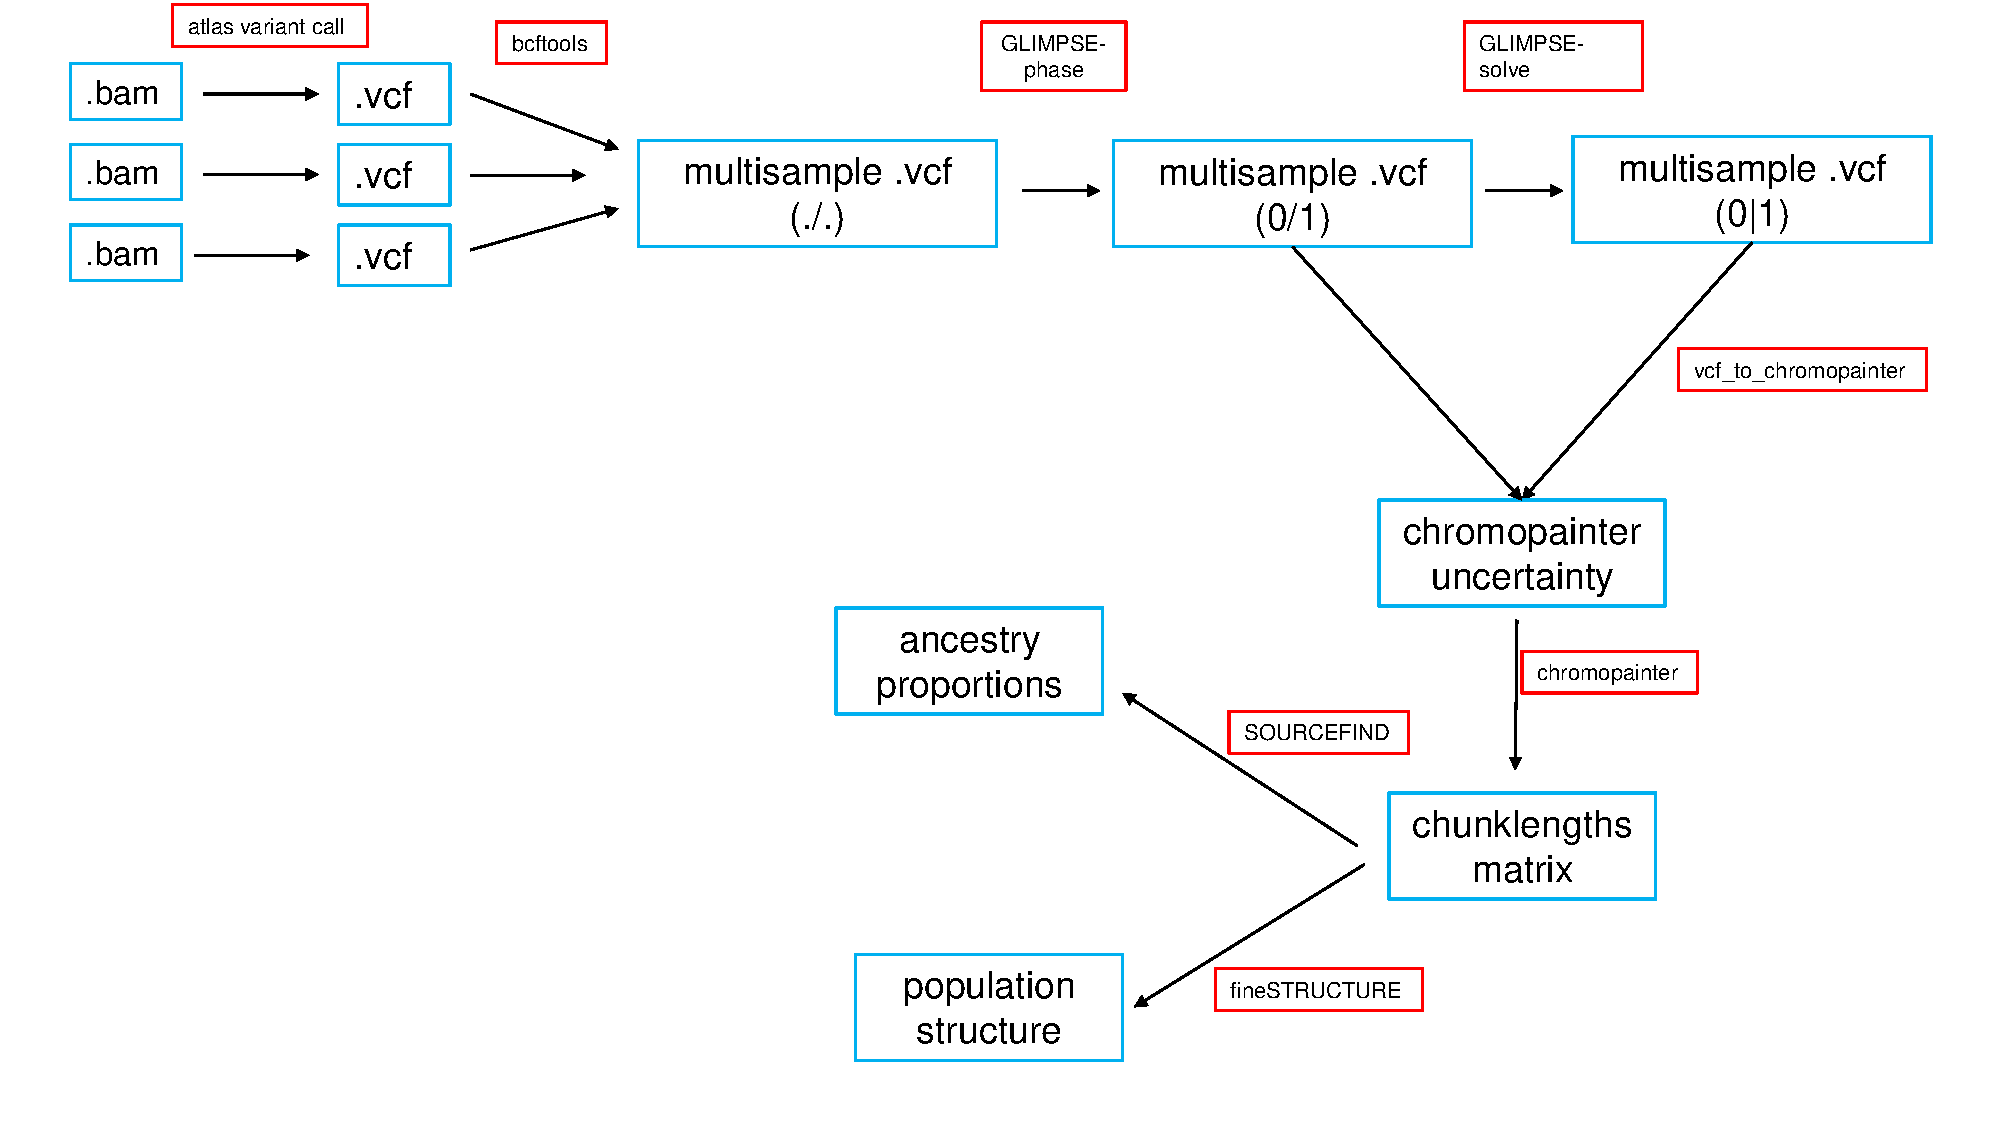
\includegraphics[width=1.0\textwidth]{../images/chapter4/workflow.pdf}
    \caption{Workflow for analysing novel and reference ancient DNA samples. Each individual .bam fie is downloaded and processed using atlas, generating vcf files containing genotype calls and genotype likelihoods at each SNP identified in the 1000 genomes project. vcf files were then merged using bcftools and phased/imputed using GLIMPSE. The phased genotypes and posterior genotype probabilities from GLIMPSE were then combined to create a ChromoPainter input file. ChromoPainter was then used to generated a .chunklengths matrix for use in SOURCEFIND.}
    \label{fig:workflow_slav}
\end{figure}


\begin{table}
\centering
\begin{tabular}[t]{lc}
\toprule
Population & \thead{Number of\\ Individuals}\\
\midrule
HB:tsi & 98\\
HB:spanish & 34\\
HB:german & 30\\
HB:french & 28\\
HB:greek & 20\\
HB:croatian & 19\\
HB:hungarian & 19\\
HB:norwegian & 18\\
HB:southitalian & 18\\
HB:polish & 17\\
HB:romanian & 16\\
HB:mordovian & 15\\
HB:cypriot & 12\\
HB:northitalian & 12\\
HB:lithuanian & 10\\
HB:siciliane & 10\\
HB:westsicilian & 10\\
HB:tuscan & 8\\
HB:irish & 7\\
HB:scottish & 6\\
HB:germanyaustria & 4\\
HB:welsh & 4\\
\bottomrule
\end{tabular}
\caption{Name of population and number of samples used in the present-day ChromoPainter analysis}
\label{table:present-day_inds_painting}
\end{table}

\subsection{SOURCEFIND ancestry proportion analysis}

I used SOURCEFIND \cite{Chacon-Duque2018} to infer the proportions of ancestry by which each target (e.g.\ ancient) individual is most related to a set of surrogate ancient populations. Each of the 47 clusters of ancient samples inferred by fineSTRUCTURE was analysed in turn, using the other 46 clusters to act as surrogates.    

Each cluster was run across three independent MCMC runs, using 50,000 burn-in iterations, 500,000 main iterations, and thinning every 5 iterations All three MCMC runs were then combined to form an MCMC list using the coda R libary \cite{oro22547} and \texttt{mcmc} function to jointly estimate ancestry proportions and empirical credible intervals for each target population. 

\subsection{MOSAIC admixture analysis}

I inferred admixture events, dates and proportions using  MOSAIC \cite{MOSAIC_2019}, performing two different analyses that mimicked the two ChromoPainter ``ancient'' and ``present-day'' paintings described above. In particular I tested each of the 5 fineSTRUCTURE clusters containing the 17 newly sequenced individuals using as surrogates: (i) 46 other fineSTRUCTURE clusters containing ancient individuals (i.e.\ from the ``ancient'' painting results) or (ii) only the 5 other Slavic ancient populations plus 49 present-day populations in Table \ref{tab:MOSAIC_pops_slav}. I assumed each target population could be formed as a mixture of both two and three admixing sources, with all other parameters left as default. 

I then performed a `present-day surrogates' analysis using a select group of present-day populations \ref{tab:MOSAIC_pops_slav} and all ancient Slavic samples. I analysed each population in turn using all other populations as surrogates.  

MOSAIC was run using default settings and the following sets of populations as targets and the following sets as surrogates. I formed each target as a mixture of both 2 and 3 mixing sources, with all other parameters left as default. Upper and lower quantiles for admixture dates were estimated using a bootstrap procedure. Other than changing the number of mixing sources, all other parameters were left as default.

\begin{table}
\small
\centering
\begin{tabular}[t]{lr}
\toprule
Population & \thead{Number of \\Individuals}\\
\midrule
HB:han & 34\\
HB:bulgarian & 31\\
HB:japanese & 28\\
HB:sardinian & 28\\
HB:russian & 25\\
HB:yakut & 25\\
HB:greek & 20\\
HB:ukrainian & 20\\
HB:croatian & 19\\
HB:hungarian & 19\\
HB:mongolian & 19\\
HB:southitalian & 18\\
HB:chuvash & 17\\
HB:polish & 17\\
HB:romanian & 16\\
HB:buryat & 15\\
HB:mordovian & 15\\
HB:altai & 13\\
HB:tuva & 13\\
HB:evenk & 12\\
HB:northitalian & 12\\
HB:cambodian & 10\\
HB:dai & 10\\
HB:hannchina & 10\\
HB:lithuanian & 10\\
HB:miao & 10\\
HB:nganassan & 10\\
HB:selkup & 10\\
HB:siciliane & 10\\
HB:tu & 10\\
HB:tujia & 10\\
HB:uygur & 10\\
HB:westsicilian & 10\\
HB:yi & 10\\
HB:belorussian & 9\\
HB:daur & 9\\
HB:oroqen & 9\\
HB:xibo & 9\\
HB:hezhen & 8\\
HB:naxi & 8\\
HB:tuscan & 8\\
HB:dolgan & 7\\
HB:chukchi & 5\\
HB:koryake & 5\\
HB:yukagir & 4\\
HB:myanmar & 3\\
HB:burya & 2\\
HB:ket & 2\\
HB:malayan & 1\\
\bottomrule
\end{tabular}
\caption{Name of populations and number of samples used in the present-day MOSAIC analysis}
\label{tab:MOSAIC_pops_slav}
\end{table}

\section{Results}


\begin{figure}[htp]
    \centering
    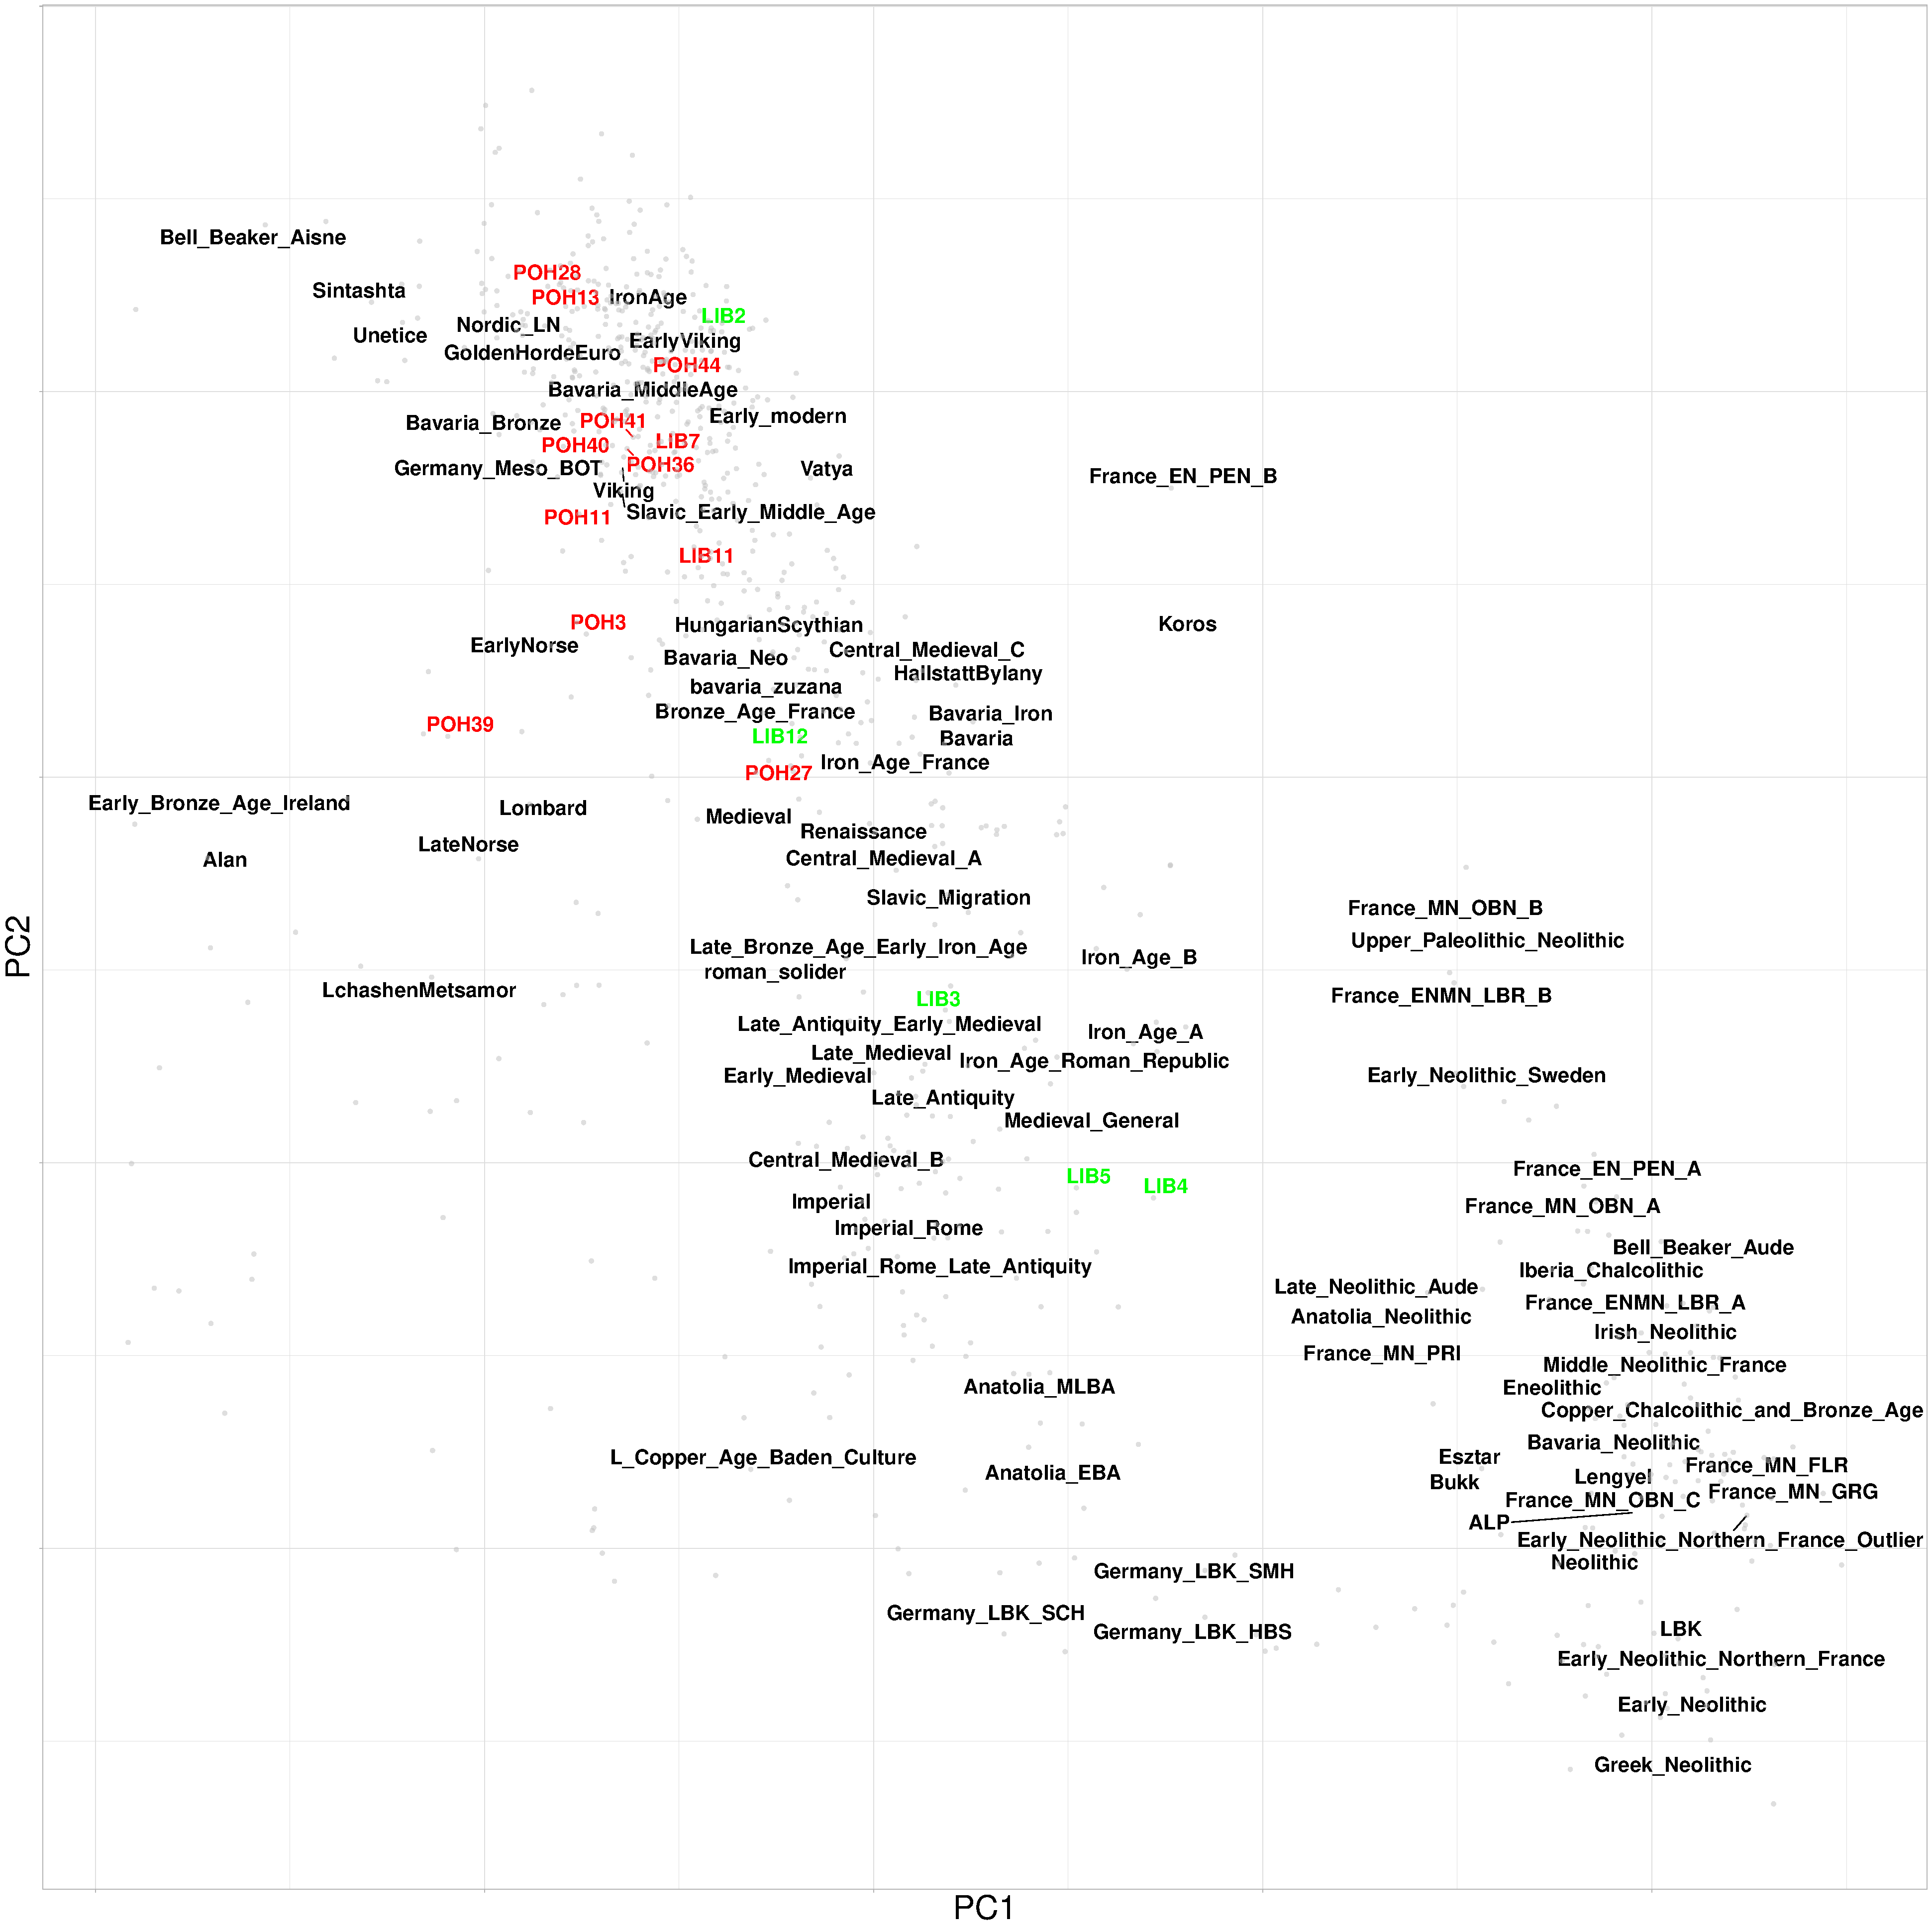
\includegraphics[width=1.0\textwidth]{../images/chapter5/plink_pca.pdf}
    \caption{Principle component plot of newly sequenced ancient samples and reference ancient individuals performed using the plink2. Green labels correspond to Migration Era samples, red labels to Early Middle Age samples and black as reference populations. The position of each reference label is the mean PC coordinates of all individuals within that population}
    \label{fig:AllChr.plink_PCA}
\end{figure}


\subsection{Mixed ancestry of Migration Period Slavs}

The Migration Period samples consisted of five individuals with radiocarbon dates corresponding to the Migration Period (348 - 509AD). Both the unlinked (Fig. \ref{fig:AllChr.plink_PCA}) and linked PCAs (Fig. \ref{fig:fs_PCA}) show that the Migration Period samples are heterogeneous and do not likely originate from the same source population. One sample, LIB2 (495AD) is located in the centre of a large cluster of contemporaneous individuals from Iron Age central and northern Europe. fineSTRUCTURE grouped LIB2 with Viking era individuals from Sweden, Denmark, Iceland, Estonia and Norway from 300-1100AD. When painted using a set of present-day reference samples, LIB2 matches the most haplotypes and clusters with Norwegians (Fig. \ref{fig:copymatrix_moderns_ancient_slavs}). Put together, this data suggests LIB2 may be a recent migrant from Viking regions. 

\begin{figure}[htp]
    \centering
    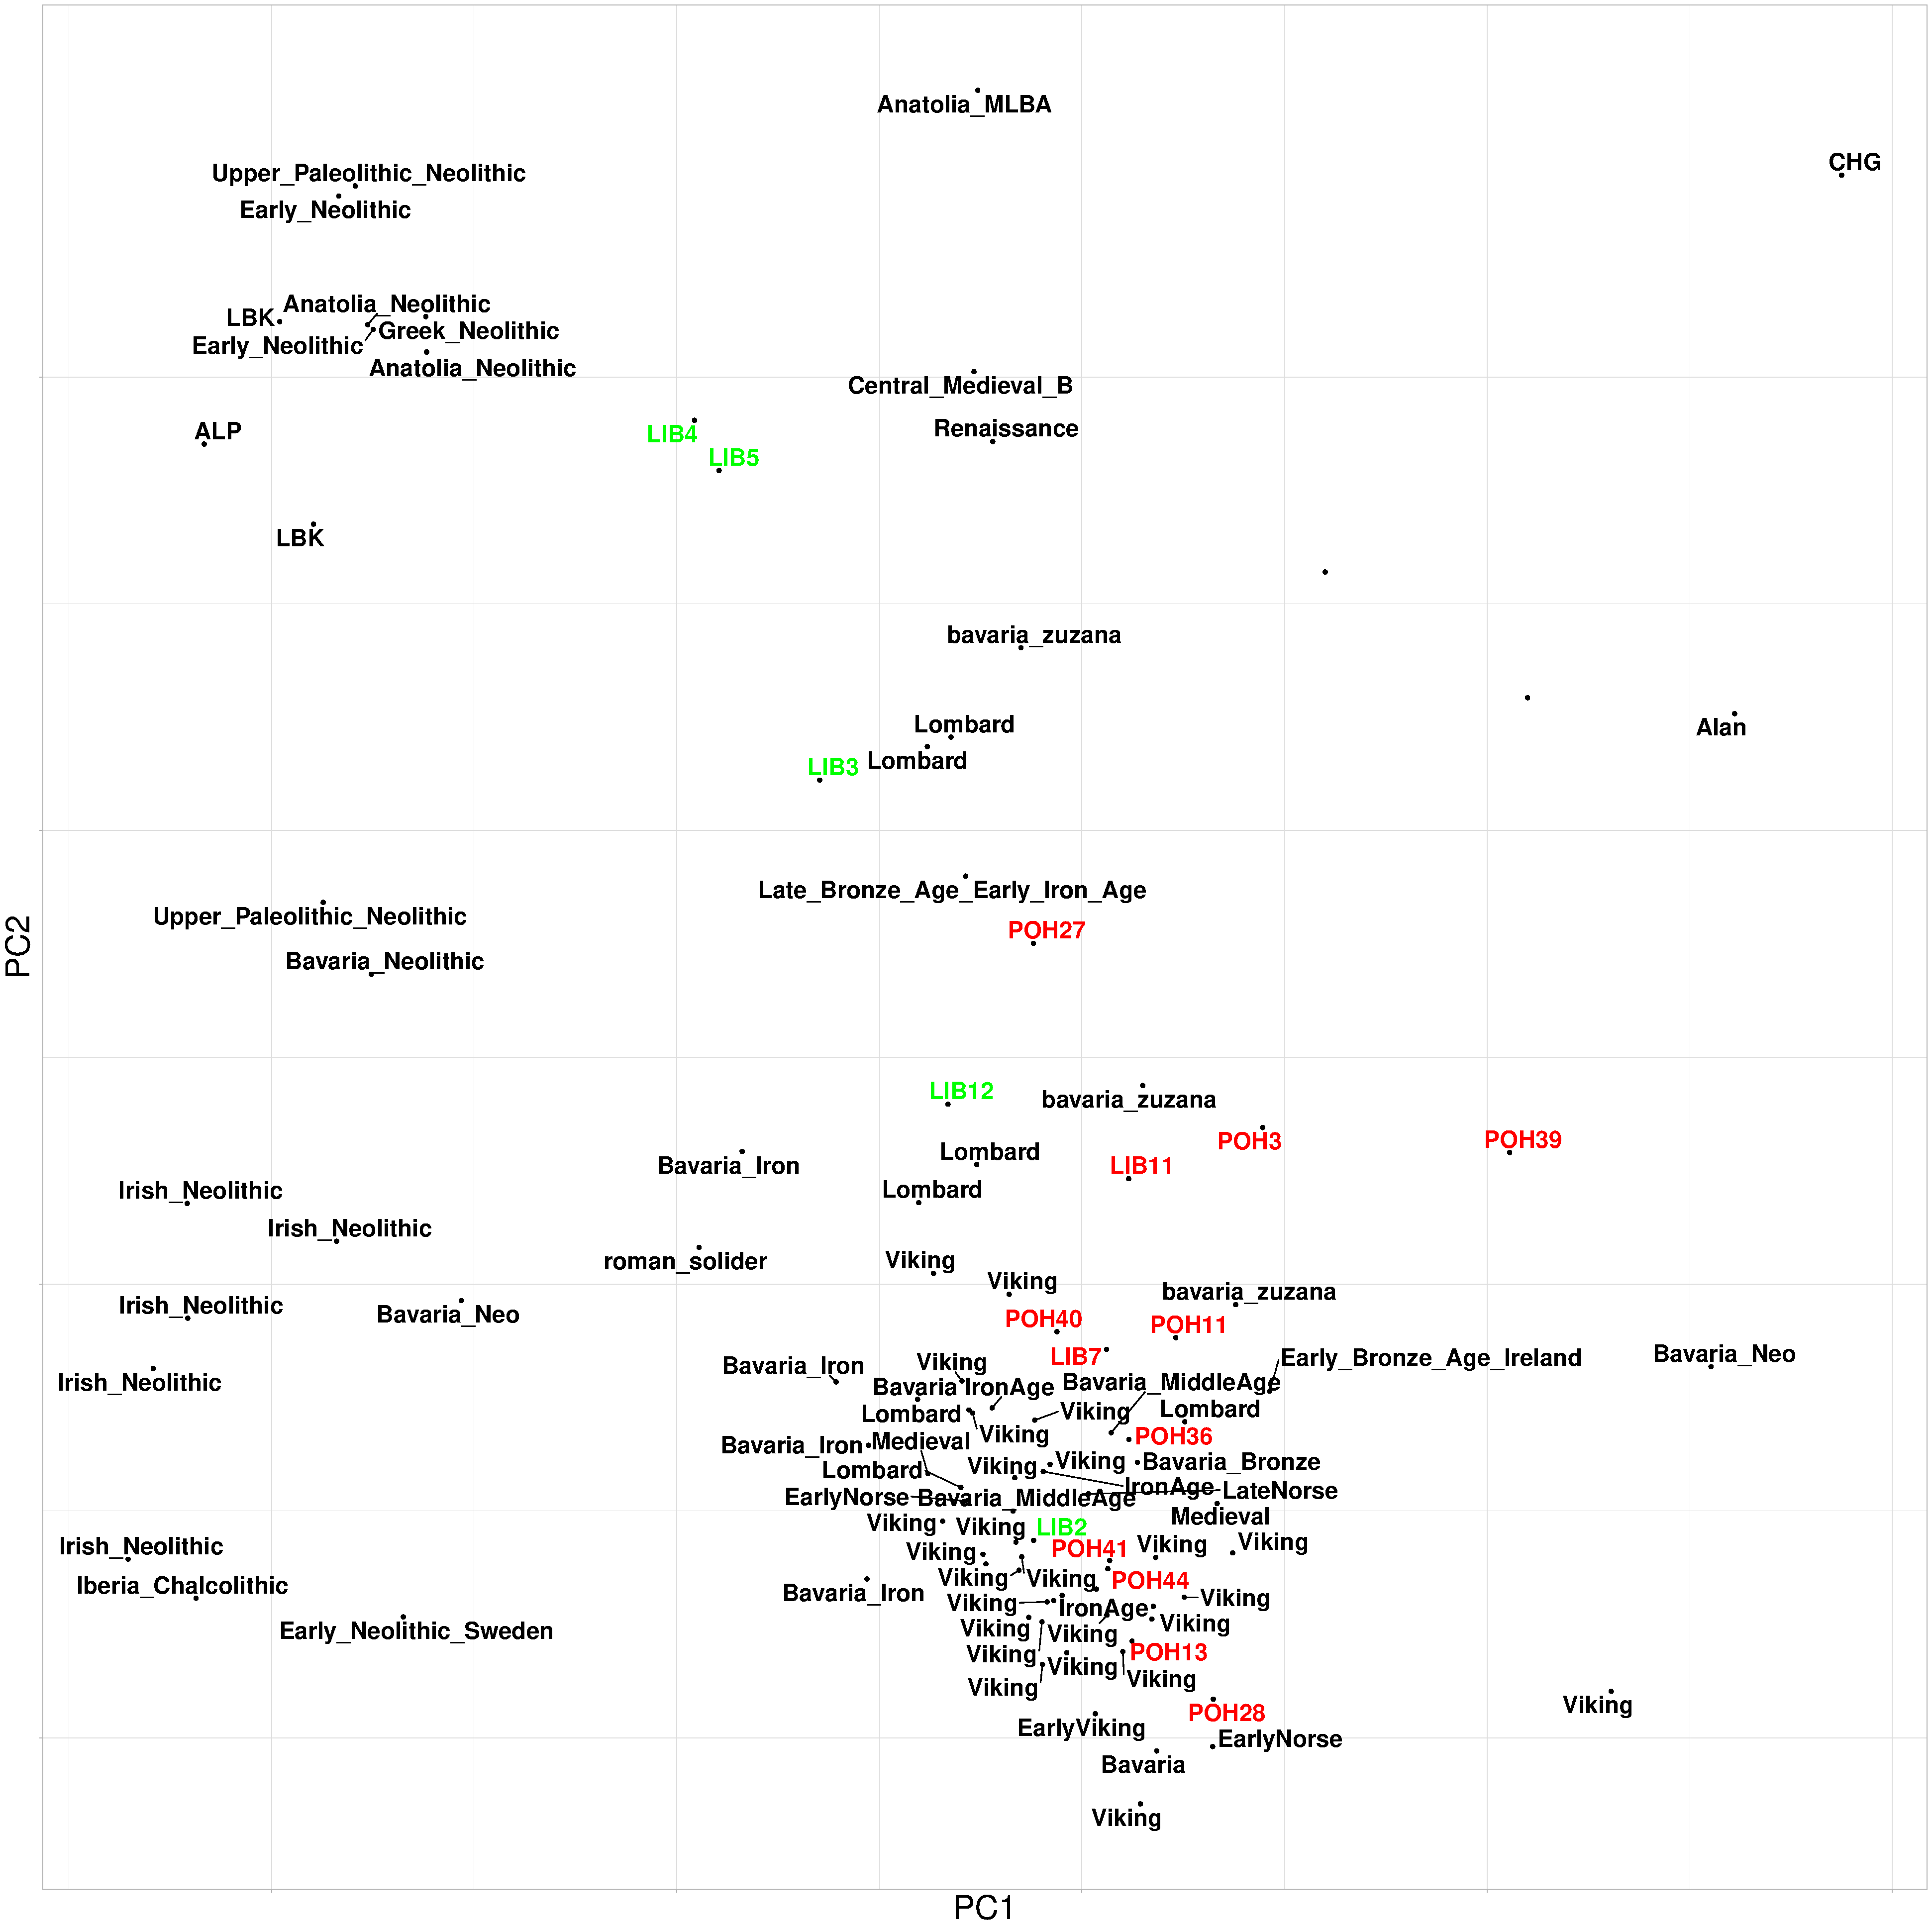
\includegraphics[width=1.0\textwidth]{../images/chapter5/fs_PCA.pdf}
    \caption{Principle component plot of newly sequenced ancient samples and reference ancient individuals performed using fineSTRUCTURE. Green labels correspond to Migration Era samples, red labels to Early Middle Age samples and black as reference populations.}
    \label{fig:fs_PCA}
\end{figure}

On the other hand, LIB4 and LIB5 are found in a fineSTRUCTURE group together with Early Iron Age and Renaissance samples from Italy, and generally show an increased affinity Neolithic / Southern European populations relative to the other Migration Period samples based on PCA results (Fig \ref{fig:AllChr.plink_PCA}-\ref{fig:fs_PCA}). All samples and their associated fineSTRUCTURE groups are found in Appendix section \ref{sec:fs_slavs_group}. 

LIB3 clusters with Lombard samples from Northern Italy (Fig \ref{fig:AllChr.plink_PCA}) in the `ancient' painting, and with Tuscans in the `present-day' painting. Finally, LIB12 displays ancestry which is more typical of the preceding Central European Bronze Age, suggesting it may represent a `leftover' from a local Bronze Age population which was unaffected by the Antiquity / Iron Age migrations to the region. It should be noted that the unlinked plink2 PCA and linked ChromoPainter PCA position LIB12 against slightly different other populations, with the unlinked PCA showing a similarity to Bronze and Iron Age French samples, and the linked PCA to Longobards and Bavarian samples. This may be caused by either the linked PCA giving higher resolution results, or giving details of a more ancient ancestral relationship.  

\subsection{Early Middle Age Slavs represent a relatively homogeneous group typical of European Middle Ages}

In comparison to the five Migration Period ancient Slavs, the 12 Early Middle Age Slavs (741-956 AD) are more homogeneous. All 12 samples cluster in the same fineSTRUCTURE group (named Slavic Early Middle Age II) (Table \ref{sec:fs_slavs_group}), alongside Viking/Medieval samples from Ukraine, Poland and Sweden. SOURCEFIND showed that the Slavic Early Middle Age II cluster derives roughly equal parts of ancestry from the clusters Viking 10C Scan I, BronzeAge I and Lombard mixed cluster (Fig. \ref{fig:SF_heatmap_slavs}). Interestingly, these three ancestry sources are similar to those identified by SOURCEFIND analyses in the Migration Period samples (Fig \ref{fig:SF_heatmap_slavs}). I tentatively therefore suggest that the Early Middle Age Slavs were formed from the mixture of `northern' (best represented by Viking) and `southern' ancestries (best represented by Lombards) onto a substrate of local Bronze Age populations.

MOSAIC admixture analysis on the Early Middle Age samples using ancient surrogates proved inconclusive. However, using present-day individuals as surrogates inferred a three-way admixture event involving sources closest to present-day day north-central Slavs (76.6\%), southern-eastern Slavs (21.9\%) and East Asians best represented by Mongolians (1.5\%) (Fig. \ref{fig:EarlyMiddleAges_MOSAIC_3way_moderns_Mu}). This admixture event was estimated to have occurred 9.4 (2.5\% 5.7gens - 97.5\% 17.9gens) generations before the samples (Fig. \ref{fig:EarlyMiddleAges_MOSAIC_3way_moderns_acoanc}), i.e.\ 476 - 732 AD. 

This admixture event is consistent with a signal inferred in both present-day day Eastern European individuals \cite{MOSAIC_2019, Hellenthal2014}. In previous studies, this admixture event was dated to approximately 1200CE (MOSAIC) and 440-1080 (GLOBETROTTER).

\begin{figure}[htp]
    \centering
    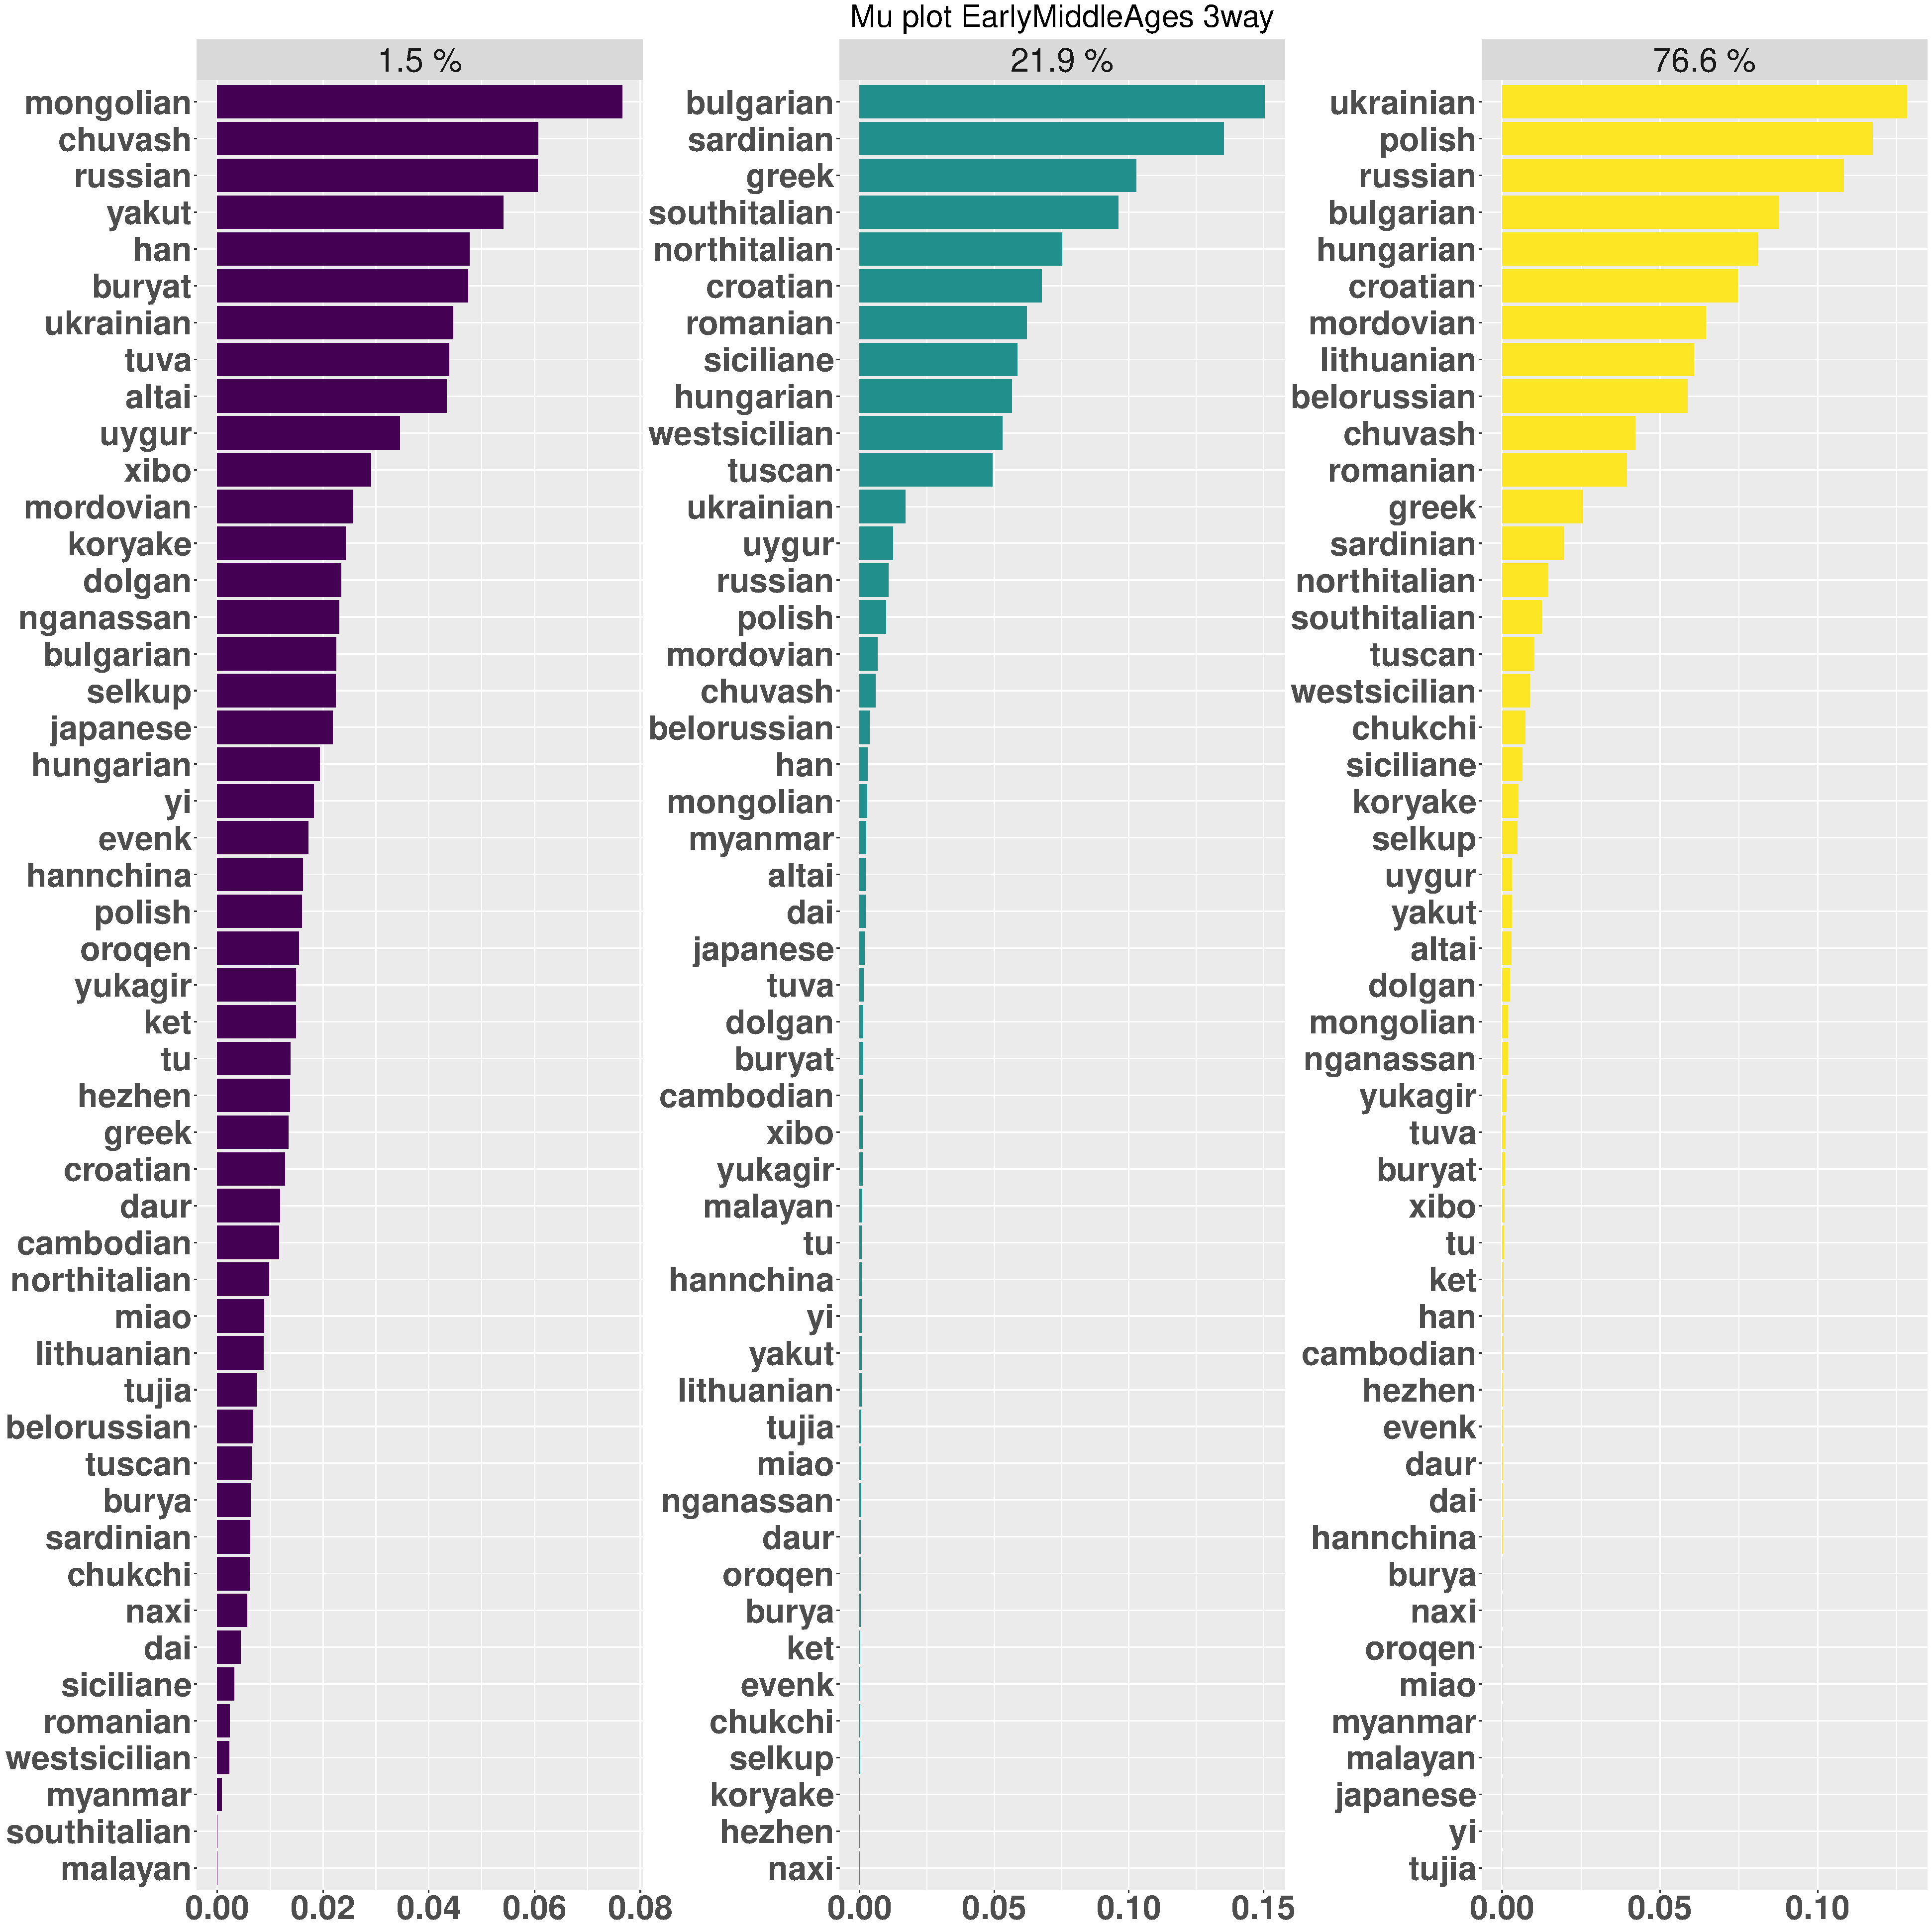
\includegraphics[width=1.0\textwidth]{../images/chapter5/Mu_plot_EarlyMiddleAges_3way.pdf}
    \caption{Copying matrix plot for sources in 3-way admixture event for Early Middle Age ancient Slavic samples. Each panel represents one of the 3 putative mixing sources. Labels above each panel gives the proportion that mixing source contributed to the Early Middle Age samples. Length of the bars within each panel represent the reflect how to best represent the relative haplotype composition of that source using the surrogate populations.}
    \label{fig:EarlyMiddleAges_MOSAIC_3way_moderns_Mu}
\end{figure}

\begin{figure}[htp]
    \centering
    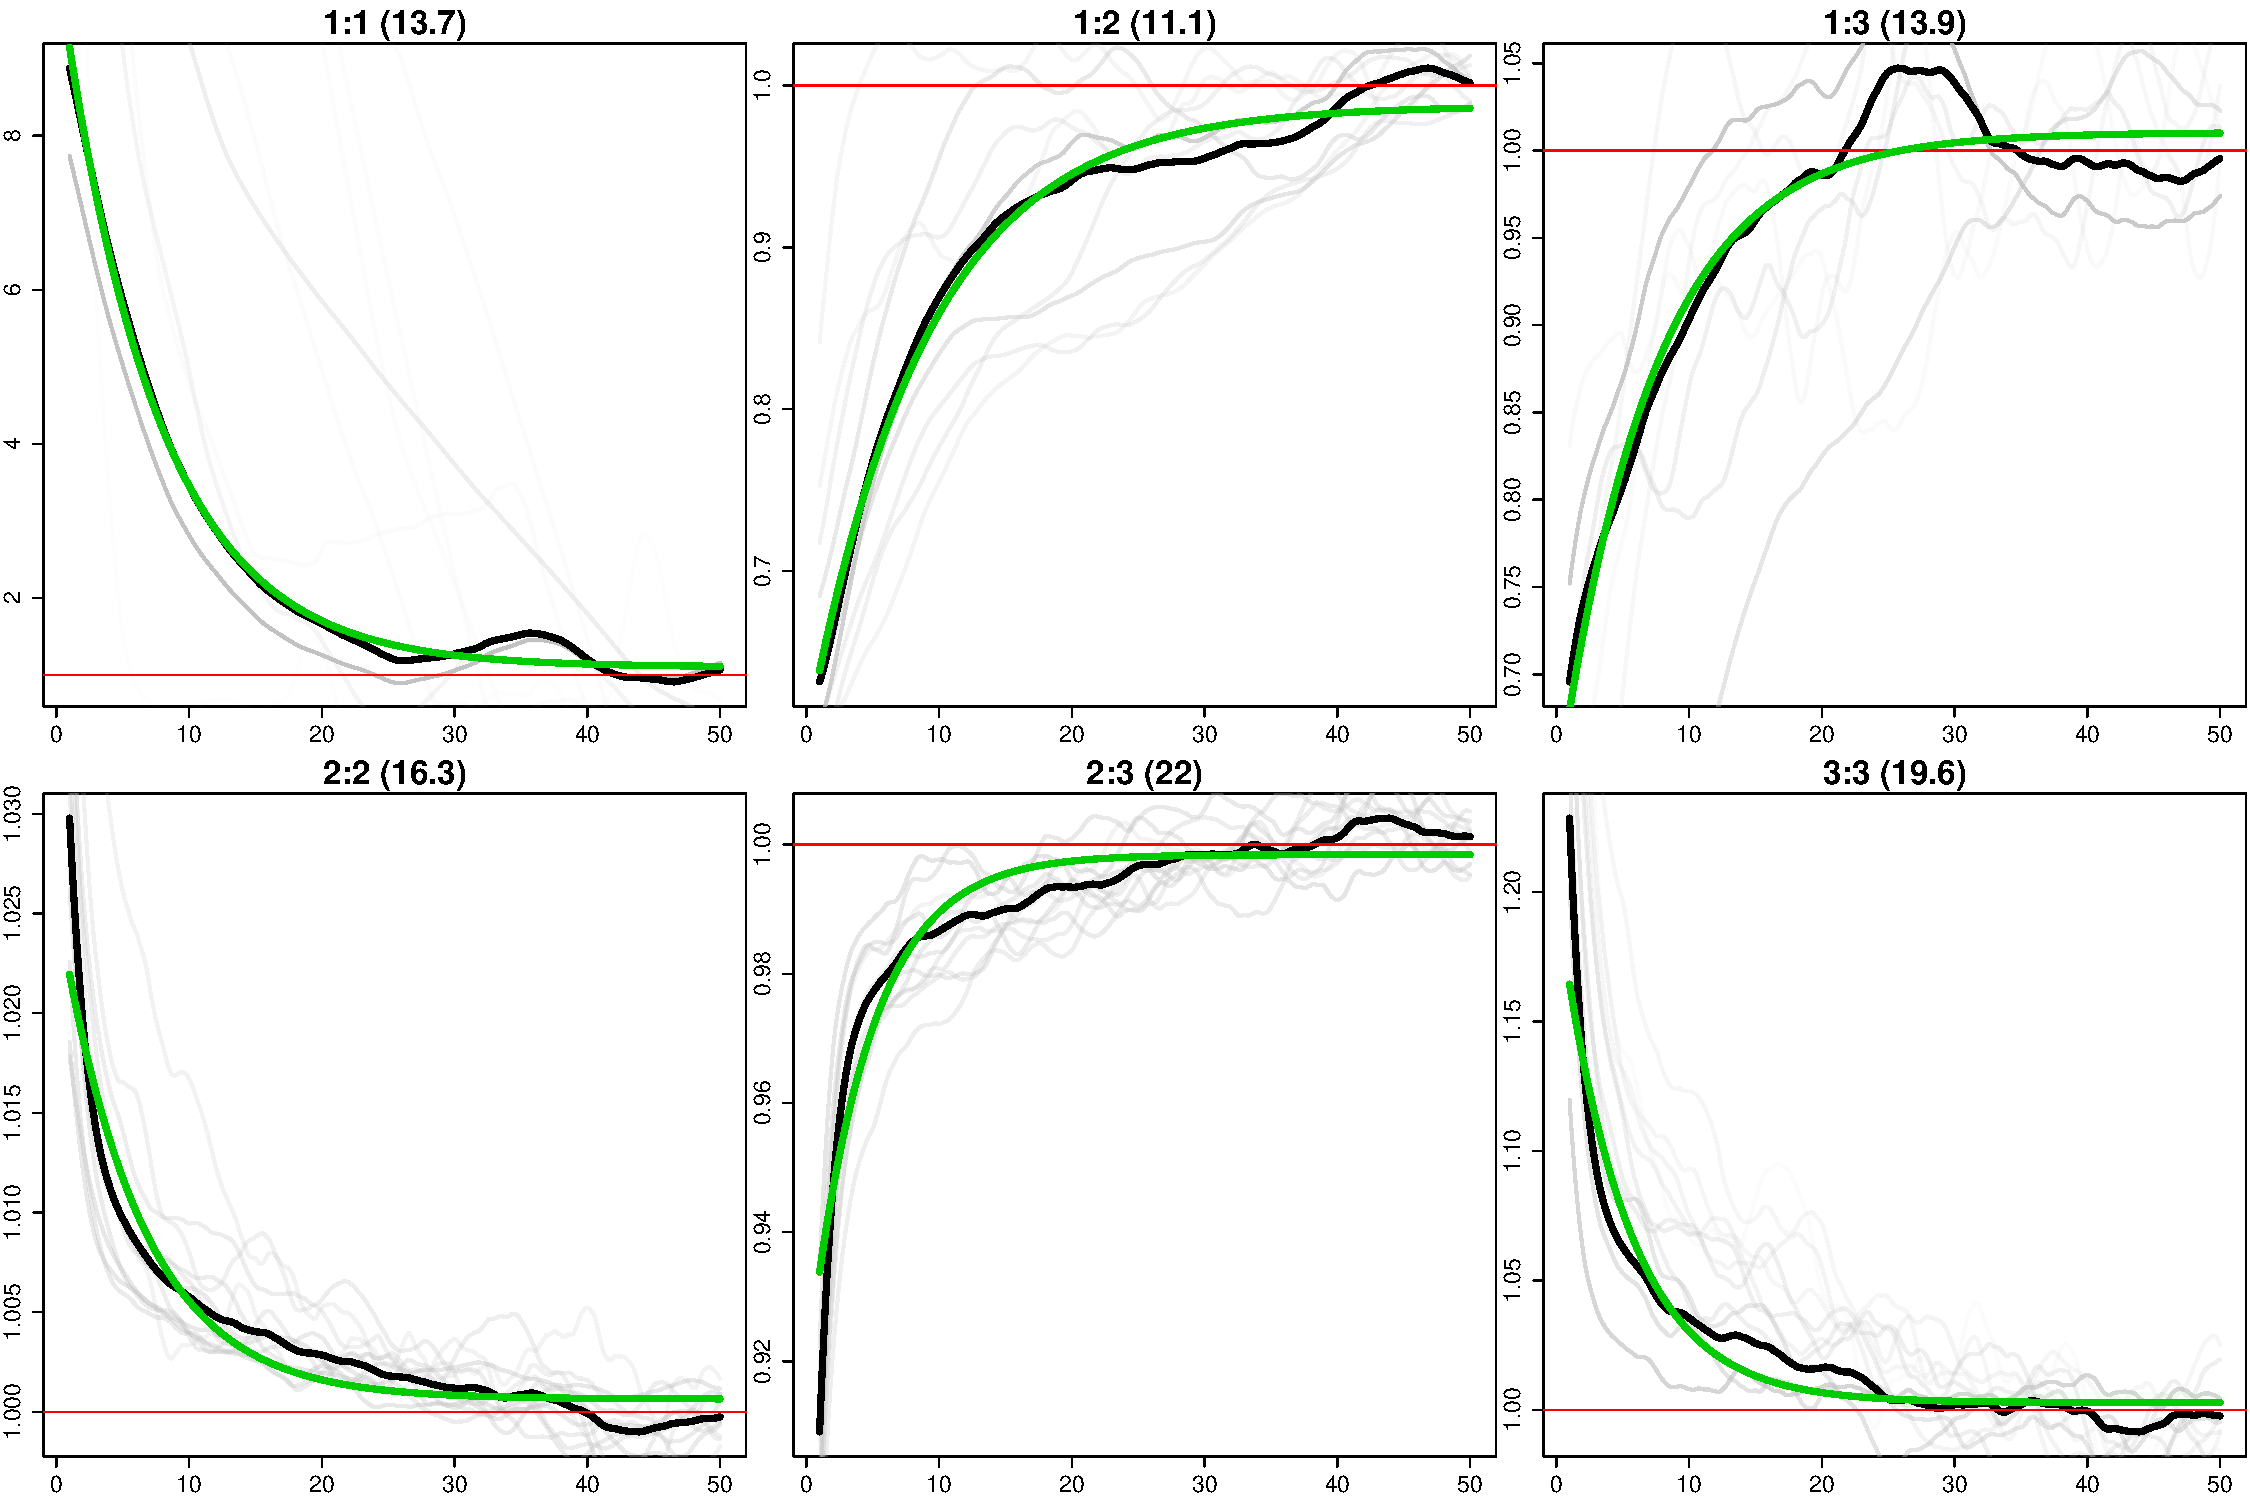
\includegraphics[width=1.0\textwidth]{../images/chapter5/EarlyMiddleAges_3way_acoanc.pdf}
    \caption{Inferred Coancestry Curves obtained from modelling Early Middle Age samples as a 3-way mixture of present-day individuals. Black lines are empirical coancestry curves across all target individuals, light grey are per individual, green is the fitted single-event coancestry curve. x-axis gives genetic distance and y-axis the probability of switching segments from source $a$ to source $b$. Sources are those given in Fig. \ref{fig:EarlyMiddleAges_MOSAIC_3way_moderns_Mu}.}
    \label{fig:EarlyMiddleAges_MOSAIC_3way_moderns_acoanc}
\end{figure}


\subsection{Assessing continuity between Early Middle Age and Migration Period samples} \label{sec:TVD_test}

To formally establish whether the Early Middle Age and Migration Period samples cluster within their respective populations to the exclusion of the other, following Leslie et al 2015 \cite{Leslie2015}, I performed a TVD permutation test. Full details of $TVD$ justification and calculation are outlined in Appendix section \ref{sec:appendixTVD}.

Using the ancients chunklengths matrix, I grouped the samples into Migration Period and Early Middle Age and calculated the average copyvectors $C_{mp}$ and $C_{ema}$ across samples within each groups. Here $C_{mp}=\{C_{mp}(1),...,C_{mp}{D}\}$, where $C_{mp}(d)$ is the average amount a Migration Period individual copies from (i.e.\ is painted by) individuals from donor population $d$. Then, I calculated the empirical TVD between the two groups as $TVD_{mp,ema} = \sum_d |C_{mp}(d) - C_{ema}(d)|$. For 10,000 iterations, I then randomly permuted the population labels among the samples and then calculated the analogous TVD, $TVD_{mp,ema}^{rand}$, between these two randomised ``populations''. I then calculated, as a p-value for the null model assuming individuals are exchangeable between the two populations, the number of randomly permuted iterations where $TVD_{mp,ema}^{rand} \geq $ $TVD_{mp,ema}$. This test supported clustering the samples into their respective groups ($p=0.0013$).

To determine the extent of continuity between the Migration Period and Early Middle Ages, I modelled each Early Middle Ages sample as a mixture of other ancients, including individuals from the preceding Migration Period, using SOURCEFIND. The proportion of ancestry derived from the Migration Period was low (mean 3.4\% , range 0.4\% - 12.5\%), suggesting that there was a relatively large scale population replacement between the two different time periods. 

\subsection{Legacy of Slavic migrations in present-day individuals}

Principle component analysis (PCA) of the present-day painting indicates genetic similarity between ancient Slavic samples from the Early Middle Ages and present-day day Slavic speaking populations (Fig. \ref{fig:chunklengths_moderns_ancients_PCA}). The Early Middle Age samples primarily cluster with present-day Polish and Belorussian individuals, but appear to fall on a cline of genetic similarity between Russians and southern Europeans. 

As with the ancients PCA, Migration Era Slavs are spread across the present-day PCA. LIB3, LIB4, and LIB5 cluster with present-day Italians, consistent with deriving a substantial ancestry component from southern European sources. LIB4 and LIB5 appear to be positioned closer to southern Italians and Greeks, whereas LIB3 is closer to northern Italian and Tuscan populations. LIB2 shows a strong affinity to present-day Norwegians, suggesting it may be a recent migrant from Viking regions. 

\begin{figure}[htp]
    \centering
    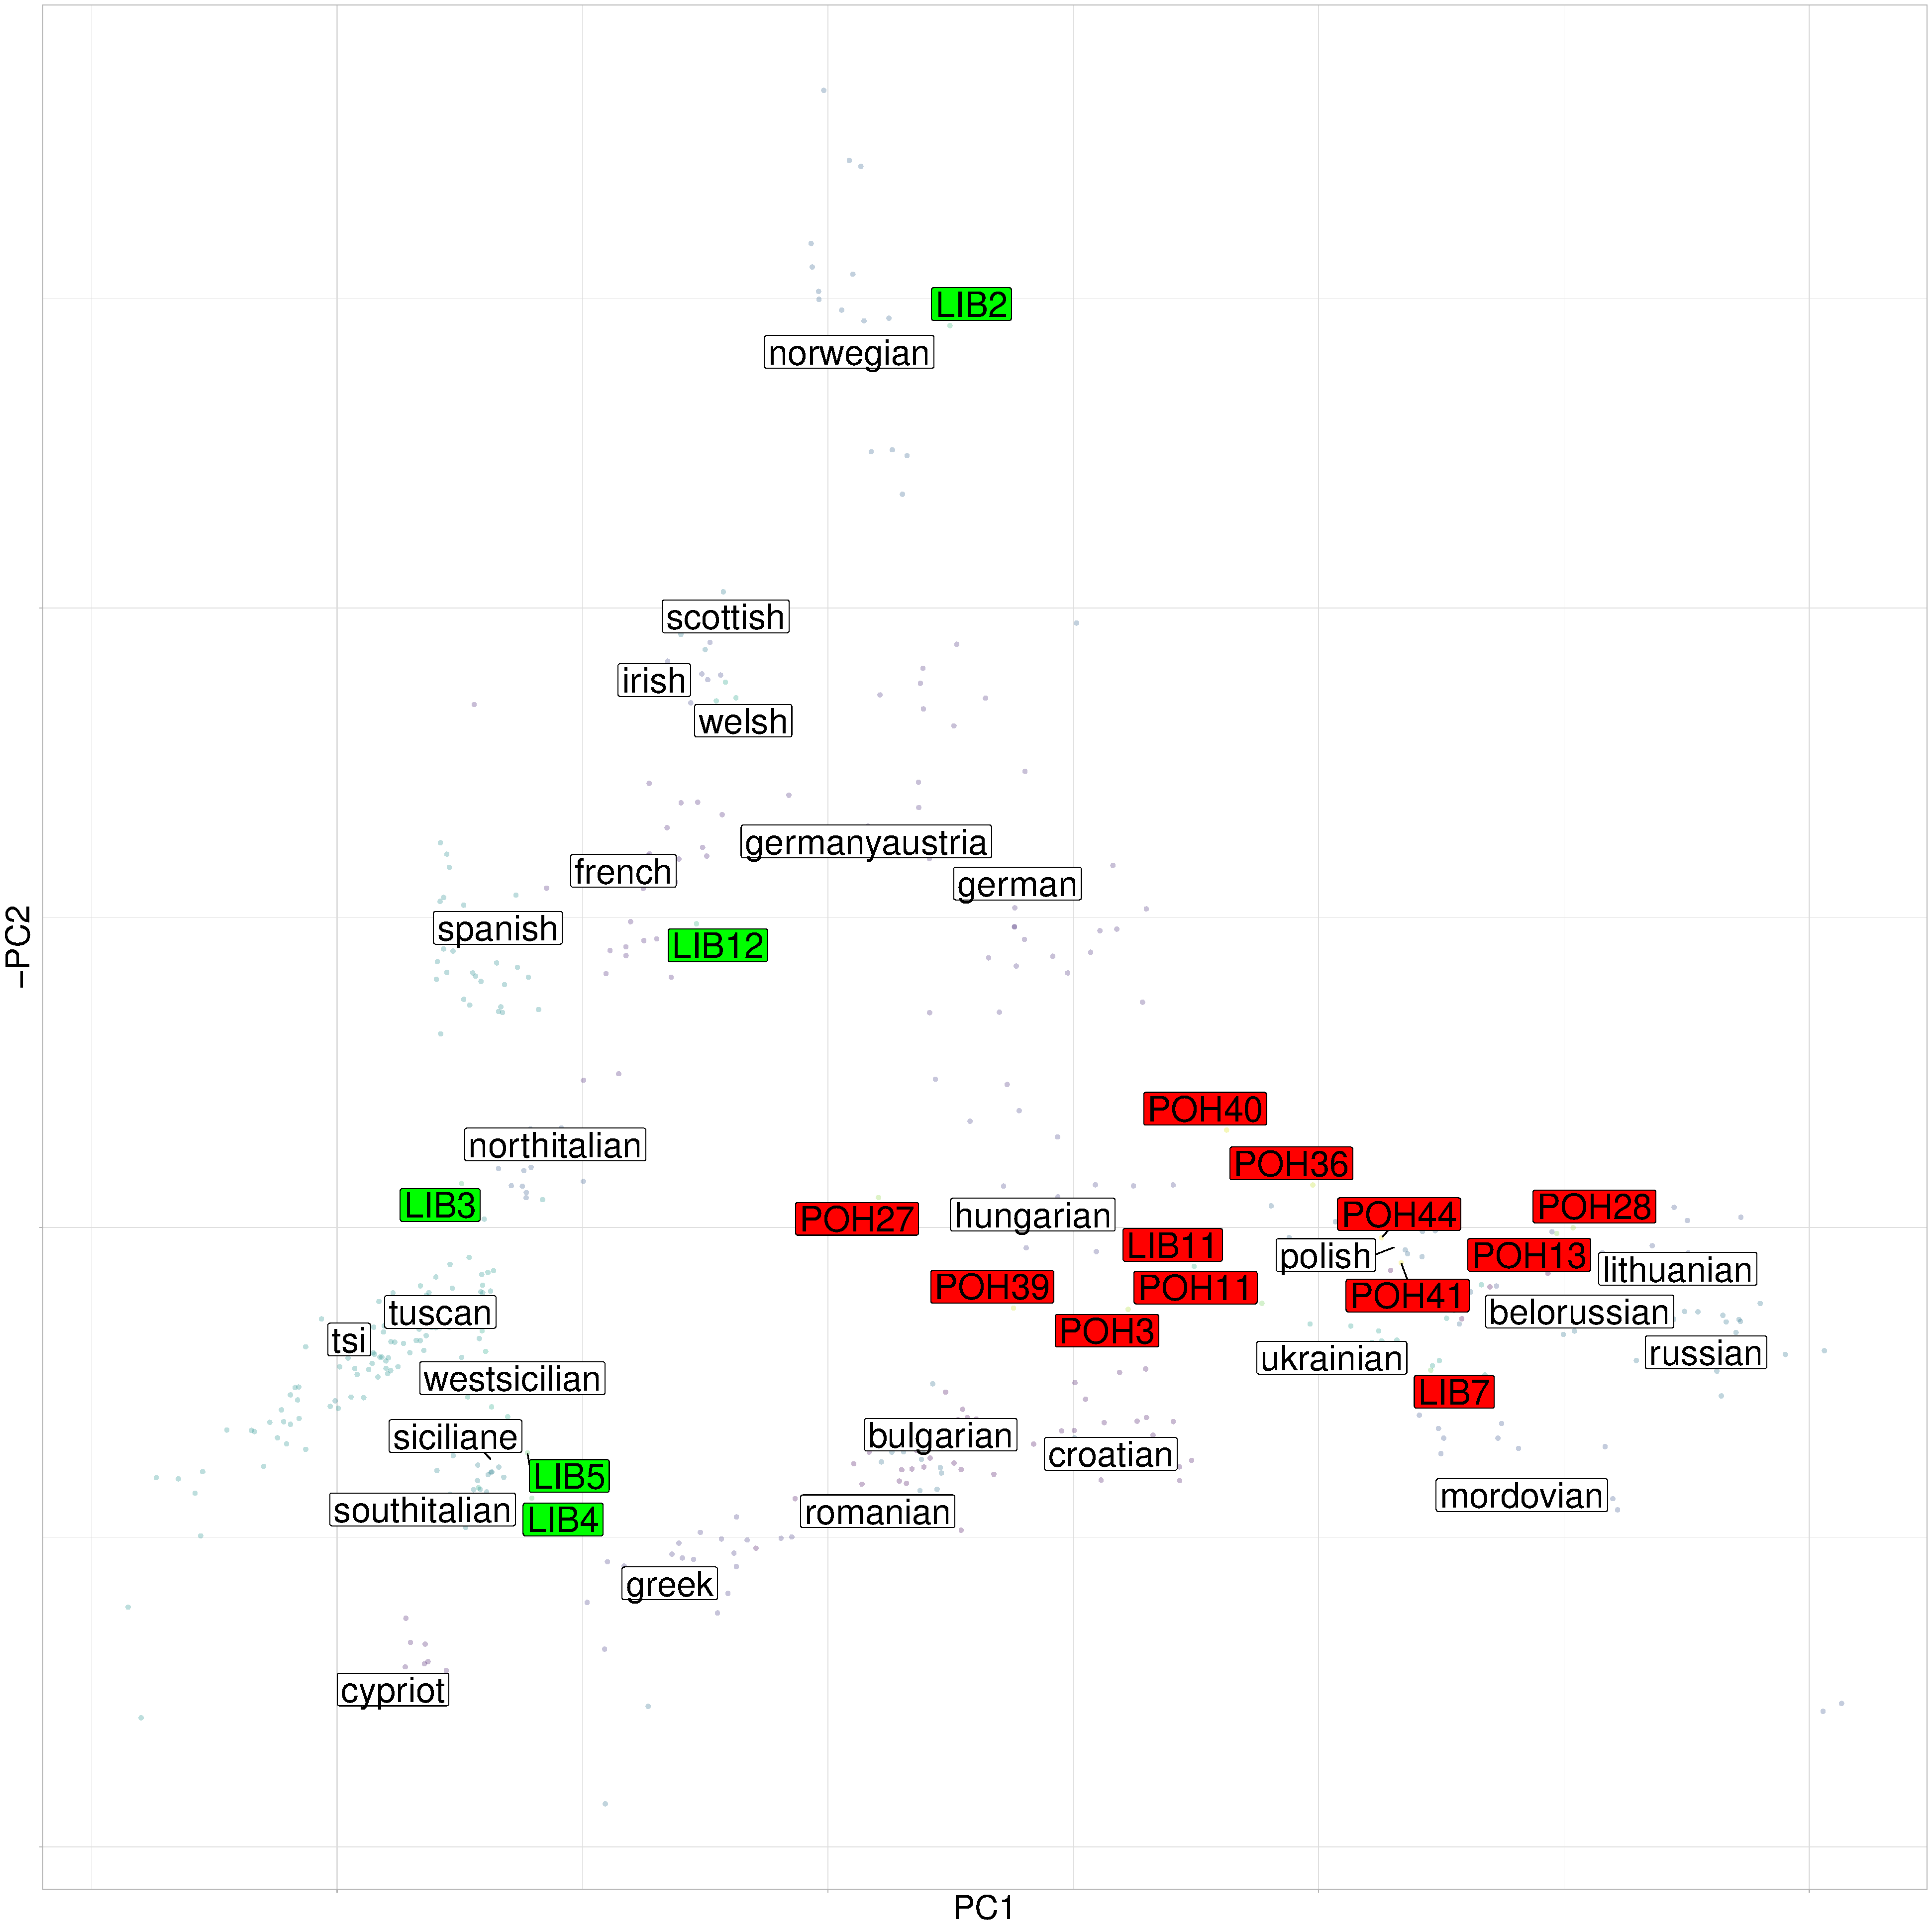
\includegraphics[width=1.0\textwidth]{../images/chapter5/chunklengths_moderns_ancients_PCA.pdf}
    \caption{Principle component plot of newly sequenced ancient samples and reference modern individuals performed using the finestructure library. Green labels correspond to Migration Era samples, red labels correspond to Early Middle Age samples and white labels correspond to reference populations. The position of each reference label is the mean PC coordinates of all individuals within that population. Transparent coloured points correspond to present-day individuals.}
    \label{fig:chunklengths_moderns_ancients_PCA}
\end{figure}

The same pattern can be observed on the raw copyvector output matrix from the present-day painting (Fig. \ref{fig:copymatrix_moderns_ancient_slavs}). In particular, Migration Era samples show little excess affinity to present-day day Slavic populations.

\begin{figure}[htp]
    \centering
    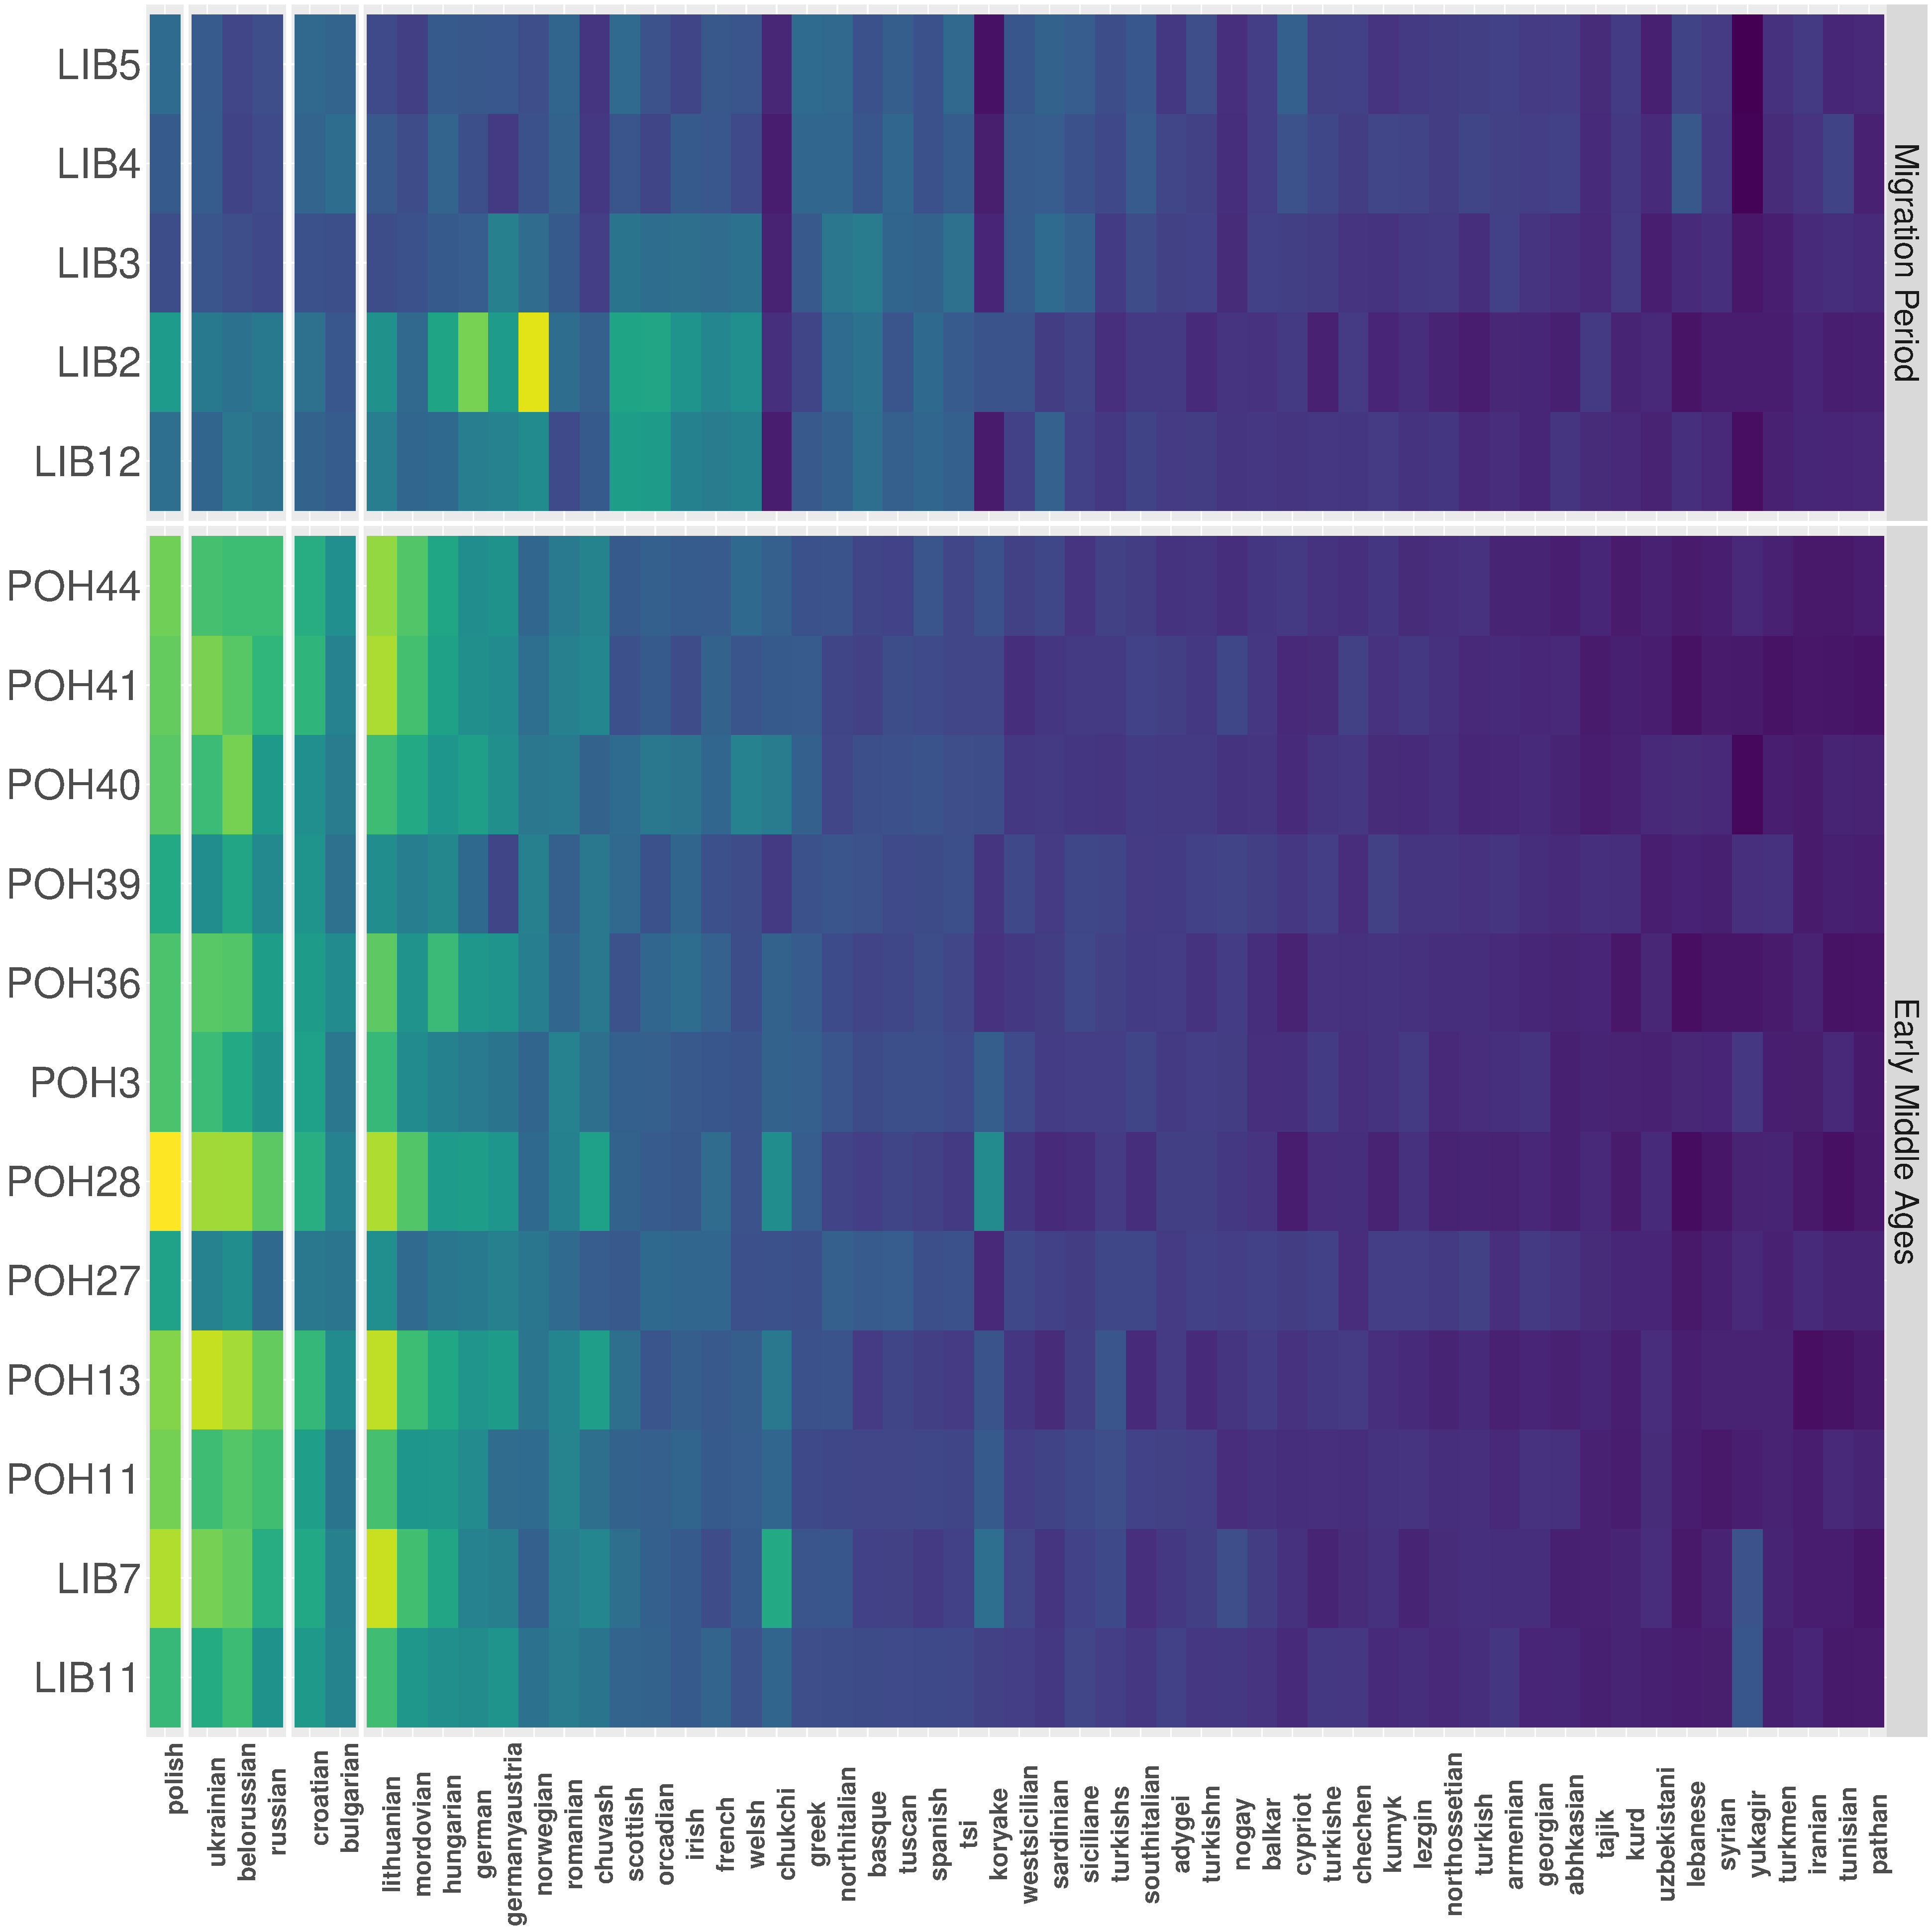
\includegraphics[width=1.0\textwidth]{../images/chapter5/copymatrix_moderns_ancient_slavs.pdf}
    \caption{Raw chunklengths matrix from the `present-day' painting. Rows correspond to different ancient recipient individuals, grouped into Migration Period and Early Middle Age period, and columns to different donor populations. Colour of cells corresponds to the total length of genome that a given donor individuals donates to that recipient, with dark/blue  indicating less sharing and light/yellow colours indicating more sharing.}
    \label{fig:copymatrix_moderns_ancient_slavs}
\end{figure} 

In contrast, the Early Middle Age samples showed a strong affinity to present-day day Slavic populations, especially Polish, Lithuanians and Mordovians. 

To confirm that the observed results were not a result of phasing or imputing ancient individuals using present-day samples, I calculated $f_{3}$ statistics on pre-imputation genotypes. Specifically, I calculated $f_{3}$, or the branch length / amount of shared drift, between a set of present-day test populations and the grouped Early Middle Age samples. The results are qualitatively similar to those obtained using ChromoPainter, with Early Middle Age ancient Slavic individuals being closest to samples from Eastern Europe (Fig. \ref{fig:f3_HB_ancient_slavs}). However, the $f_{3}$ results do not appear to show the same degree of geographical structure; for example, Early Middle Age have a more positive $f_{3}$ with present-day Irish individuals than with some present-day Slavic-speaking groups such as Croatians, perhaps reflecting relatively higher genetic drift in the Irish population.

\begin{figure}[htp]
    \centering
    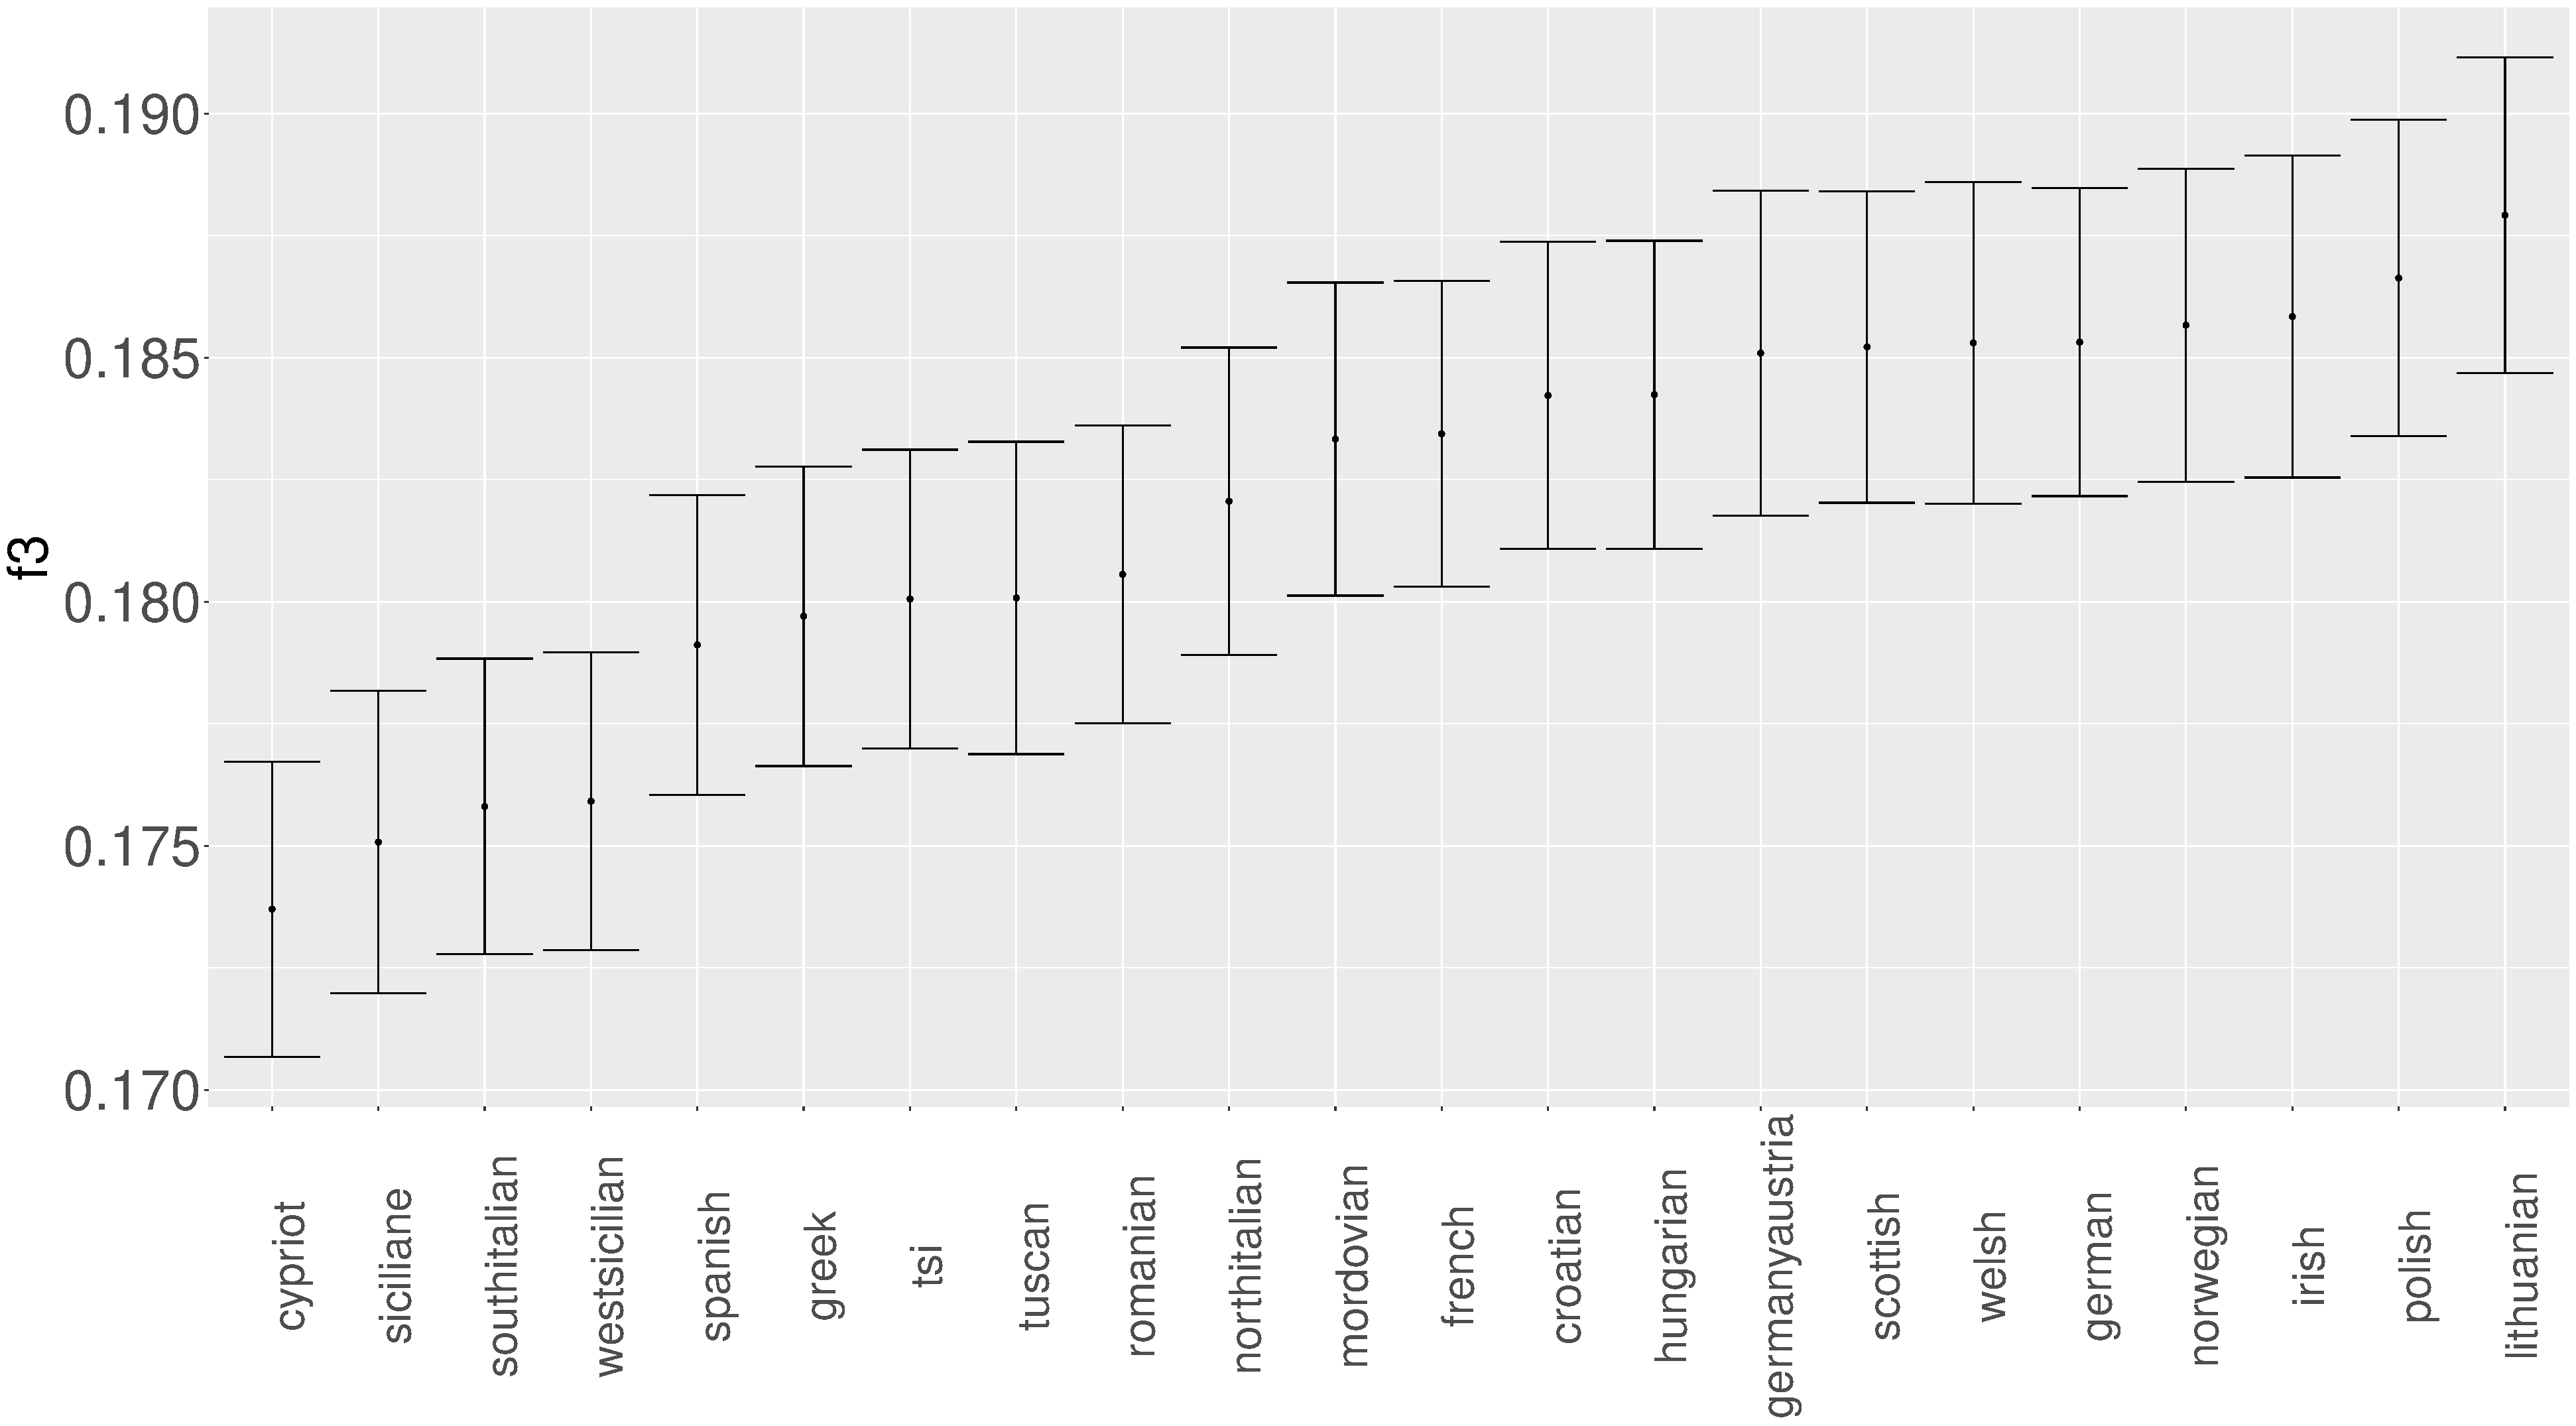
\includegraphics[width=1.0\textwidth]{../images/chapter5/f3_HB_ancient_slavs.pdf}
    \caption{$f_{3}$ statistics in the form of $f_{3}(EMA, present-day;mbuti pygmy$), where \textit{present-day} is different present-day European population. Error bars rerpesent $\pm*2$ standard error.}
    \label{fig:f3_HB_ancient_slavs}
\end{figure}


\subsection{Genetic structure and admixture events of present-day Slavic people}

fineSTRUCTURE clustering on the 17 ancient samples with 21 present-day European populations gave results similar to those obtained from visually inspecting the chunklengths matrix in Fig \ref{fig:copymatrix_moderns_ancient_slavs}. Among Migration Period samples, LIB2 and LIB12 cluster with north-west European groups, LIB3 clusters with Tuscany, and LIB4/LIB5 cluster with Spain. The present-day Slavic populations I had data for fall into two fineSTRUCTURE clades consistent with geography: (1) Croatians and Bulgarians (``south-east''), (2) Belarusians, Lithuanians, Polish, Russians and Ukrainians (``east''). Of the Early Middle Age samples, three (POH3, POH39, POH27) cluster into `south-east' Slavic clade, with the remaining seven clustering into the `east' clade. These results are consistent with the a hypothesis that the structure in present-day Slavic populations has been present since the Early Middle Ages.


\begin{figure}[htp]
    \centering
    \includegraphics[width=1.0\textwidth]{../images/chapter5/tree_with_ancients.pdf}
    \caption{Population dendrogram generated by the fineSTRUCTURE tree building algorithm. Labeled tips refer to the primary population(s) represented in that clade. present-day non-Slavic populations shown in black. `south-east' Slavs highlighted in cyan and `north-west' Slavs highlighted in yellow. Migration period individuals superimposed in green and Early Middle Age samples superimposed in red. Read fineSTRUCTURE paper for description of edge values. Note: some tips contained more than one population but were not included as labels to save space.}
    \label{fig:tree_with_ancients}
\end{figure} 


Previous studies have identified admixture events in present-day Slavic populations involving an east-Asian source approximately 440 - 1080 CE \cite{Hellenthal2016, MOSAIC_2019}. In previous sections, I showed that this signal exists in the Early Middle Age ancient samples and is best characterised by populations from present-day Mongolia (Fig. \ref{fig:EarlyMiddleAges_MOSAIC_3way_moderns_Mu}). I employed MOSAIC \cite{MOSAIC_2019} to replicate the results of Hellenthal et al (2014) and Myers and Salter-Townshend (2019) and determine whether a similar admixing source is present in the ancient populations. I analysed all present-day populations (Table \ref{tab:MOSAIC_pops_slav}) and ancient Slavic populations in turn. For the ancient Slavic samples, I grouped all Early Middle Age samples together and grouped LIB3, LIB4 AND LIB5 together as the Migration Period samples. 

When considering 2-way admixture event, all of the tested populations (both ancient and present-day), bar the Migration Period, showed evidence of an admixture event involving a minor source that has the lowest $f_{st}$ with present-day Uygurs. The dates and bootstrapped confidence intervals are given in Fig. \ref{fig:MOSAIC_admixture_dates_plot}. Other than Norwegians and Croatians, whose dates are later and earlier respectively, the dates for other populations appear to be constrained around 1250 CE. This date is similar, but slightly later than that obtained from Hellenthal et al (2014), who estimate it to be 440 to 1080 CE.

\begin{figure}[htp]
    \centering
    \includegraphics[width=1.0\textwidth]{../images/chapter5/MOSAIC_admixture_dates_plot.pdf}
    \caption{MOSAIC inferred 2-way admixture dates with bootstrapped 97.5\% and 2.5\% CI). Vertical green lines correspond to radiocarbon estimated dates of Migration Period samples and red lines equivalent for Early Middle Age samples. Estimated dates obtained by assuming an average generation time of 26 and date of birth of 1950 for present-day samples. Populations are coloured based on whether they show signals of east Asian admixture (blue) or not (green). Source populations are those given in table \ref{tab:MOSAIC_pops_slav}.}
    \label{fig:MOSAIC_admixture_dates_plot}
\end{figure} 

Of the present-day Slavic speaking populations, Belorussian, Polish and Ukrainian, show evidence of a 3-way admixture event, in which the middle component has the lowest $f_{st}$ with Migration Era ancient samples (Fig. \ref{fig:Fst_plot_HB:lithuanian}). The major component has a low $f_{st}$ with Early Middle Age Slavs. This suggests that the formation of present-day Slavic populations could have occurred via admixture events involving Migration Era individuals with high levels of Southern European ancestry, Middle Age Era samples which show a strong affinity to present day eastern Europeans, and a small but significant east Asian source best represented by present-day Uygurs. It seems possible this ancestry may have been transmitted via Finno-Ugric speaking populations which contain Siberian ancestry, with admixture dates beginning approximately 3500 years ago \cite{Lamnidis2018}.

These results are similar to those in the Middle Age samples (Fig. \ref{fig:EarlyMiddleAges_MOSAIC_3way_moderns_Mu}), though dates are more recent in the present-day samples (Fig \ref{fig:MOSAIC_admixture_dates_plot}), suggesting recent admixture in present-day populations may be masking the older signals we see in the Early Middle Ages group.

\begin{figure}[htp]
    \centering
    \includegraphics[width=1.0\textwidth]{../images/chapter5/Fst_plot_HB:belorussian.pdf}
    \caption{$1 - F_{st}$ between 3 inferred mixing sources for present-day Belorussians. Each panel represent a different mixing source. Each bar gives the value $1-F_{st}$ between that samples population and the mixing source. Higher values of $1-F_{st}$ suggest that source is well represented by a particular population. }
    \label{fig:Fst_plot_HB:lithuanian}
\end{figure} 

\section{Summary of Results and Discussion}

Referring back to the questions posed in the introduction.

I found that the Migration Period samples, relative to the Early Middle Age samples, show a high degree of diversity in terms of ancestry, with affinities to present-day samples varying from Norway to southern Italy. On the other hand, fineSTRUCTURE analysis on the `ancients' painting grouped all Early Middle Age samples together, showing that they represent a group of samples which likely share common ancestry. Consistent with this, the Early Middle Age samples showed evidence of east Asian admixture, a signal that was not present in the Migration Period samples. These results suggest a population turnover may have occurred between approximately 500-700 AD, the time period between the Migration Period and Early Middle Age. However, based on MOSAIC results of present day populations, a model of mixture between sources close to Migration Era, Early Middle Age and east-Asians seems plausible (Fig. \ref{fig:Fst_plot_HB:lithuanian}).


All of the Early Middle Age samples showed a high genetic similarity to present-day Slavic and non-Slavic speaking populations from eastern Europe, such as Poland and Lithuania (Fig. \ref{fig:copymatrix_moderns_ancient_slavs}). This is in stark contrast to the Migration Period, who all fell on a cline of genetic similarity between present-day Scandinavian and Mediterranean populations (Fig. \ref{fig:chunklengths_moderns_ancients_PCA}). Whilst I did not explicitly test a model of genetic continuity, these results provide strong evidence a higher degree of continuity existed between the Early Middle Ages and the present-day, relative to between the Migration Period and Early Middle Ages.

Finally, a joint fineSTRUCTURE analysis which included both ancient and present-day samples showed that present-day Slavic speakers can be split into  `north-west' and `south-east' groups, and that different Early Middle Ages samples had differing affinities to these groups (Fig \ref{fig:tree_with_ancients}). 

I found strong evidence that LIB2 was a recent migrant from Viking regions. There are many sources which detail the links between the Viking and Slavic peoples towards the end of the first millennium \cite{duczko2004viking, peterson2016vikings}. However, most evidence suggests these links occurred later than the estimated radiocarbon date of LIB2. For example, it is known that the Scandinavian colonists settled in present-day Russia as early as 750 AD, whilst LIB2 was samples at approximately 495 AD. Therefore, we could suggest that this is evidence of an earlier link than previously known. In their large-scale study of ancient DNA of Viking samples from across Europe, Margaryan et al (2020) present Viking samples and ancestry in Estonia, but not until the beginning of the 8th Century, some 200 years after the estimated date of LIB2.  

I also found evidence of southern European-like ancestry in three (LIB3, LIB4 and LIB5) Migration Period samples. The appearance of southern European-like ancestry in Central Europe in the first millennium is similar to a signal found in a study exploring the ancestry of individuals with elongated skulls in medieval Bavaria (approximately 500AD) \cite{Veeramah2018}. It was shown that particular individuals harbour substantial Southern-European ancestry from outside of Bavaria, closest to individuals from present-day Greece and Turkey. There are at least two possible explanations for the presence of this ancestry in the Migration Era samples. Firstly, LIB3, LIB4 and LIB5 may be similar migrants to the region. This is consistent with the fact they are all female; Veeramah et al (2018) showed that there was a tendency for females to migrate from southern regions, perhaps related to the formation of strategic alliances.

The results from the analysis of combined ancient and present-day genomes are consistent with those from Kushniarevich et al (2015) \cite{Kushniarevich23015} who determined that Eastern (Russia, Belarus, Ukraine) and Western (Polish) central European Slavs form a cluster to the exclusion of Southern Slavs (Croatia, Bulgaria), whilst also remaining distinct from geographically proximate Germanic (German/Austrian) and Baltic (Lithuanian) populations. This is also consistent with results from Veeramah et al 2011, who showed that Sorbs, a west-Slavic population found between Poland and Germany, have a much stronger affinity to more distant Slavic populations from Czechia than to more proximate Germans \cite{veeramah2011genetic}. 


\chapter{General Conclusions}
\label{chapterlabelConclusions}

\section{General summary}

In this thesis, I have explored the use of ChromoPainter on ancient DNA samples and present-day samples which contain sparsely genotyped markers. I evaluated the impact of coverage on all steps of the analysis pipeline, from imputation and phasing to ChromoPainter and SOURCEFIND analysis, focussing on the trade-off between potential gains from leveraging haplotype information and potential reference bias. I then applied my findings to two novel and one publicly available dataset(s). 

In Chapter 2, I showed that the copyvectors of $\geq$0.5x downsamples show a high correspondence with the same sample at full coverage (Fig. \ref{fig:CP_correlation_allSamples_0.1x_0.5x_30x}), when painted using both ancient and present-day donors. 

Disappointingly, my several attempts to improve the performance of ChromoPainter on 0.1x and 0.5x samples were not successful, including filtering the SNPs used using different criteria (Section \ref{sec:Solutions}). This was surprising, as my work and that of others \cite{hui2020evaluating} showed that filtering SNPs on e.g. genotype probabilities could substantially reduce the overall fraction of incorrectly imputed genotypes. I also found evidence of imputation bias towards the reference (Fig. \ref{fig:imputed_nonimputed_donation}).

Using present-day samples, I also showed that you can gain haplotype information using sparsely genotyped data with (presumably) perfect information at each SNP. Specifically, individuals from Cornwall and Devon can be distinguished genetically with $>$90\% accuracy using only 1565 500-kb regions that contain $\approx$ 6.6 SNPs on average (i.e.\ $\approx$ 40,000 SNPs in total) (Table. \ref{table:windows_power_table_DevCorn}). A similar classification rate was found for distinguishing Mandenka from Senegal and Yoruba from Nigeria, with $>$90\% accuracy when using 1565 500-kb regions of $\approx$ 8 SNPs (Table \ref{table:windows_power_table_ManYor}). However, it appears current imputation approaches do not make reliable enough genotype calls on aDNA samples with $<$0.5x average coverage to provide many 500-kb windows with correctly called (and no incorrectly called) genotypes. Perhaps this is not surprising, as my exploration of 587 available ancient DNA samples revealed that genomes with 0.5x coverage have $<$1500 500-kb regions with 12 SNPs covered by even two reads (Figure \ref{fig:avg_good_windows}), making calling heterozygotes challenging (or impossible) throughout the genome.

In Chapter 3, I explored African ancestry in U.K. Biobank samples. Following from my Chapter 2 findings, I showed that it is possible to recover substantial haplotype information with only a fraction of the total number of SNPs usually used. Being able to use fewer SNPs in an analysis will allow different datasets to be merged and jointly analysed, opening up a larger array of questions to be answered, whilst also significantly reducing the computational footprint of an analysis. I found that in terms of fine-scale population assignment, performing imputation on non-European samples using a predominantly European reference panel biases ChromoPainter analyses towards reference populations (Fig \ref{fig:imputed_excess_copying_pops}), as does performing analysis in unlinked mode (Table \ref{table:TVD_copying}). Indeed, performing analysis on a majority imputed SNPs is more harmful for accuracy than using 70,000 SNPs in unlinked mode. This suggests that imputing to combine data from different SNP arrays may actually be more harmful than using a relatively small number ($<$100,000) of overlapping non-imputed SNPs when inferring fine-scale ancestry patterns.

My analyses showed that approximately 4\% of U.K. Biobank participants have at least 50\% African ancestry. Within this set of individuals, genetic ancestry from West Africa was very prevalent, consistent with historical events (Fig \ref{fig:haplotype_sharing_map_zoomed_II}). In particular, I found that there was over ten times the number of individuals with at least 50\% ancestry from Yoruba than there was the next most common ancestry. 

In Chapter 4, I analysed novel ancient DNA datasets from Bavaria with the samples spanning almost 7000 years of history. The analysis of ancient Bavarian samples recapitulated previous research which identified admixture events between early farmers and local hunter-gatherers, and the presence of steppe-related ancestry in the Late Neolithic. However, it also provided some less expected results, showing that samples with extremely different ancestries cohabited the same cave and the same time period. I also identified ancestry most closely related to Iron Age Italian sourced which arrived in Bavaria during the Iron Age, but was not present in the preceding Bronze Age, which may be related the migrations of Lombard populations. Future studies could increase the number of ancient sample sequenced from Bronze and Iron Age Bavaria in order to constrain the date the ancestry appears and source of origin. Finally, I showed that early Germanic and Slavic samples from the Middle Ages, which could not be distinguished using other ancient samples, showed strong genetic differences when analysed using present-day data (Fig. \ref{fig:germanic_slavic_HB_sharing}). Whilst I was able to identify structure down to the level of individuals countries, the lack of data from different regions in Germany meant that I was not able to determine whether there was fine-scale differential relatedness to the ancient samples for different German states. 

My final Chapter analysed the differences between Migration Era and Early Middle Age samples from Czechia. The data revealed that whilst different Migration Era samples displayed genetic affinities to a wide spectrum of other ancient and present-day populations, the Early Middle Age individuals were relatively more homogenous and broadly showed strong similarity to present-day Slavic speaking populations (Fig. \ref{fig:copymatrix_moderns_ancient_slavs}). However, fineSTRUCTURE analysis using present-day Slavic and non-Slavic speaking populations clearly showed that present-day Slavic speaking populations can be split into south-east and north-west clusters, with different ancient samples showing different affinities to each cluster. Lastly, I provided evidence that previously reported \cite{Hellenthal2014, MOSAIC_2019} signals of east-Asian admixture in eastern-European populations was also present in the Early Middle Age ancient Slavic samples (Fig. \ref{fig:EarlyMiddleAges_MOSAIC_3way_moderns_acoanc}. Although the five Migration Era samples represented an array of ancestries present in Czechia during that period, the sample size (n=3 at most) per sub-population was too low to reliably infer admixture events.  

\section{Recommendations}

My recommendations for analysing low coverage data are as follows:

\begin{enumerate}
\item Include samples with at least 0.5x mean coverage. Samples below this coverage (0.1x) show effects of coverage-related bias in copyvector estimation, SOURCEFIND analysis and positions on a PCA. 
\item When merging data from different genotyping arrays, it is preferable only to retain directly genotyped SNPs rather than imputing missing ones using a reference panel. This applies when the total number of directly genotyped SNPs is at least 45,000 (Fig. \ref{fig:Devon_Cornwall_TVD_reduced_assignment}).
\end{enumerate}

\section{Limitations of work and future avenues of research}


Firstly, I did not consider ancient samples from Africa. This is in part because of a lack of high coverage samples from Africa (Mota being the highest coverage at ~10x) and the vast majority of ancient DNA samples from western Eurasia. I expect results to differ when considering African samples. Africans harbour more diversity and have lower levels of background LD \cite{bosch2009decay} and thus would be expected to match shorter segments to other individuals. Imputation accuracy would likely be lower, in part because of less LD and higher genetic diversity, but also because less of the total proportion of genetic diversity is present in reference panels. Finally, the large population turnovers in Africa (e.g. the Bantu expansions) mean that many pre-Bantu ancient samples may harbour diversity that does not exist in present-day individuals. Therefore, it is possible that coverage greater than 0.5x may be necessary to accurately analyse African samples with ChromoPainter. 

I did not evaluate the effect of coverage on either fineSTRUCTURE or GLOBETROTTER analysis. This is because GLOBETROTTER struggles to identify admixture events in single samples and I only had a single downsample for each individual and level of coverage. To accurately estimate admixture events, segments of DNA within an individual copied from different populations need to be identified. Such segments may be particularly hard to identify in low coverage samples, as the segment boundaries may contain low-coverage SNPs.   

I didn't use the largest reference panel (HRC) to impute ancient samples, due to technical challenges in obtaining access to the data and so likely underestimate the potential accuracy of imputation on low coverage samples. Thus, future work should examine the scale of improvements in imputation accuracy when using extremely large reference panels. For example, plans to sequence the whole-genomes of 200,000 U.K. Biobank participants would provide an unparalleled resource to impute variants in ancient samples of western European ancestry. 

Whilst my attempt at incorporating genotype likelihoods into the ChromoPainter process only provided very modest improvements, the fact that this approach has been successful in other methods \cite{ngsLD, vieira2016estimating, Meisner719, Lipatov023374} suggests that in theory it should also be applicable to Chromosome painting. Future work on ChromoPainter could explore the reason why this did not work and suggest alternate ways in which to account for the uncertainty associated with low coverage data. Studies could also interrogate the performance of ChromoPainter on the range of coverages between 0.1-0.5x. Recent research has argued it is possible to infer ancestral relationships between samples as low as 0.1x in coverage, although only for particular applications such as demographic change \cite{colate}.

On the other hand, methodological advances in laboratory DNA extraction techniques, DNA enrichment and sequencing technologies and library preparation for ancient samples may mean that all samples can be sequenced to a high enough coverage that coverage-related effects are inconsequential. 





\addcontentsline{toc}{chapter}{Appendices}

% The \appendix command resets the chapter counter, and changes the chapter numbering scheme to capital letters.
%\chapter{Appendices}
\appendix
\chapter{Datasets used}

This appendix described the different datasets used in analyses performed in this thesis. It includes datasets of both modern and ancient genomes.

\section{Ancient reference dataset} \label{section:AncientReferenceDataset}

This section describes the generation of the dataset of reference ancient individuals used in Chapters 2, 4 and 5. 

\begin{table}
\centering
\begin{tabular}[t]{lcl}
\toprule
Paper & \thead{Number of\\ Samples} & Reference\\
\midrule
Allentoft 2015 & 20 & \cite{Allentoft2015}\\
Antonio 2019 & 134 & \cite{antonio2019ancient}\\
Broushaki 2016 & 1 & \cite{Broushaki2016b}\\
Brunel 2020 & 58 & \cite{Brunel12791}\\
Cassidy 2015 & 4 & \cite{Cassidy368}\\
deBarrosDamgaard 2018a & 34 & \cite{deBarrosDamgaardeaar7711}\\
deBarrosDamgaard 2018b & 58 & \cite{de2018137}\\
Gamba 2014 & 10 & \cite{Gamba2014}\\
Gunther 2015 & 2 & \cite{gunther2015ancient}\\
Hofmanova 2016 & 5 & \cite{Hofmanova2016}\\
Jones 2015 & 2 & \cite{Jones2015}\\
Lazaridis 2014 & 1 & \cite{Lazaridis2014}\\
Marchi 2020 & 4 & \cite{marchi2020mixed}\\
Margaryan 20 & 442 & \cite{margaryan2020population}\\
Berger unpublished & 14 & NA\\
Olade 2014 & 1 & \cite{olalde2014derived}\\
Rivollat 20 & 101 & \cite{rivollat2020france}\\
Sanchez-Quinto 2019 & 7 & \cite{sanchez2019megalithic}\\
Seguin-Orlando 2014 & 1 & \cite{Seguin-Orlando2014}\\
Veeramah 2018 & 1 & \cite{Veeramah2018}\\
Hofmanova unpublished & 37 & NA\\
\bottomrule
\end{tabular}
\caption{Name of paper, number of samples and reference for all literature ancient samples used in analyses}.
\label{tab:AncientReferenceDataset}
\end{table}

For each of the samples in Table \ref{tab:AncientReferenceDataset}, the following steps were taken to produce ChromoPainter input.

\begin{enumerate}
\item Each \texttt{.bam} was processed with \texttt{PicardTools ValidateBam} \cite{Picard2018toolkit} task to ensure no files were corrupted or contained incorrect read group information.
\item Each \texttt{.bam} file was processed with atlas (version 1.0, commit f612f28) pipeline \cite{Link2017} (\url{https://bitbucket.org/wegmannlab/atlas/wiki/Home}). For .bam file, I estimated post-mortem damage (PMD) patterns using atlas \texttt{estimatePMD} task. Recalibration parameters were then estimated using atlas \texttt{recal} task. Finally, both the recalibration and PMD parameters were given to the \texttt{callNEW} task which produces genotype calls and genotype likelihood estimates for each downsampled and full coverage .bam. For this stage, I made calls at the 77,818,345 genome-wide positions present in the phase 3 thousand genomes project \cite{1000GenomesProjectConsortium2015}. This was done to reduce the risk of calling false-positive non-polymorphic sites. This resulted in a \texttt{.bcf} file for each ancient sample. 
\item All \texttt{.bcf} files were split into chromosomes and all samples from the same chromosome were merged. Imputation and phasing was performed with GLIMPSE (version 1.1.1). I followed the steps laid out in the GLIMPSE tutorial (\url{https://odelaneau.github.io/GLIMPSE/tutorial_b38.html}). First, I used \texttt{GLIMPSE\_chunk} to split up each reference chromosome into chunks, keeping both \texttt{--window-size} and \texttt{--buffer-size} to 2,000,000, their default settings. Across all chromosomes, this produced 936 chunks of an average 2.99Mb long. I used the b37 genetic map supplied by GLIMPSE for the \texttt{--map} argument. 

Each chunk was then imputed separately using \texttt{GLIMPSE\_phase} using the same 1000 genomes dataset as a reference. Default settings and the supplied b37 genetic map were used. This stage both imputes missing genotypes and generates a set of haplotype pairs which can be sampled from in a later step to produced phased haplotypes.

\texttt{GLIMPSE\_ligate} was then used to merge the imputed chunks back to form single chromosomes using the default settings and the supplied b37 genetic map. 

Haplotypes were then sampled using \texttt{GLIMPSE\_sample} to produce a .vcf with phased haplotypes for each individual, again using default settings and the supplied b37 genetic map. 

Consequently, the output of GLIMPSE is i) unphased genotype calls with posterior genotype likelihoods and ii) phased haplotypes.


\item Finally, the posterior genotype likelihoods and phased haplotypes were combined to generate ChromoPainterUncertainty output using a custom script (\url{https://github.com/sahwa/vcf_to_chromopainter}).



\end{enumerate}



\section{30x 1000 genomes dataset} \label{section:1000genomes}


Samples from \cite{byrska2021high}.

This dataset consists of 3,202 modern individuals from 26 worldwide populations, sequenced to a targeted depth of 30x coverage. The downloaded dataset was aligned to the gr38 reference genome. Samples were downloaded to the UCL Computer Science cluster by myself from the ftp mirror. The following steps were taken to process the data before being used as an imputation reference. 

\begin{enumerate}
\item Filtered such that SNPs with only 2 alleles were retained
\item Performed a liftover to hg19 using LiftoverVcf from picard tools \cite{Picard2018toolkit}
\item Filter again for SNPs with only 2 alleles
\item Phase using shapeit4, using the `sequencing' parameter and setting --pbwt-depth 4.
\item Remove duplicated SNPs using bcftools norm \cite{li2009sequence} 
\item Use Beagle's conform-gt utility to ensure reference alleles were consistent with the previous 1000 genomes build. This was done because all previous datasets I have compiled were also conformed to the previous 1000 genomes build. 
\end{enumerate}

\begin{table}
\centering\begingroup\fontsize{9}{11}\selectfont

\begin{tabular}[t]{cc}
\toprule
Population Code & Number of individuals\\
\midrule
ACB & 116\\
ASW & 74\\
BEB & 131\\
CDX & 93\\
CEU & 179\\
CHB & 103\\
CHS & 163\\
CLM & 132\\
ESN & 149\\
FIN & 99\\
GBR & 91\\
GIH & 103\\
GWD & 178\\
IBS & 157\\
ITU & 107\\
JPT & 104\\
KHV & 122\\
LWK & 99\\
MSL & 99\\
MXL & 97\\
PEL & 122\\
PJL & 146\\
PUR & 139\\
STU & 114\\
TSI & 107\\
YRI & 178\\
\bottomrule
\end{tabular}
\endgroup{}
\caption{Population codes and number of individuals for each 1000 genomes populations.}
\end{table}

Population codes and populations can be found at \url{https://www.coriell.org/0/Sections/Collections/NHGRI/1000genome.aspx?PgId=664&coll=HG}.





\section{Human Origins dataset} \label{HumanOriginsAppendix}

This dataset consists of 560,420 SNPS and 5998 individuals from 509 worldwide populations. It has a particularly large number of samples from West and East Africa; in particular, Cameroon, Ethiopia, Nigeria and Ghana. 

\begingroup\fontsize{8}{10}\selectfont

\begin{longtable}[t]{lll>{\raggedright\arraybackslash}p{9em}r}
\toprule
Region & Country & Populations & Ref & sum\\
\midrule
Africa & Algeria & Algerian & Lazaridis et al 2014 & 4\\
Africa & Algeria & Mozabite & Lazaridis et al 2014 & 21\\
Africa & Botswana & Gana & Lazaridis et al 2014 & 7\\
Africa & Botswana & Gui & Lazaridis et al 2014 & 7\\
Africa & Botswana & Hoan & Lazaridis et al 2014 & 6\\
Africa & Botswana & Ju hoan South & Lazaridis et al 2014 & 5\\
Africa & Botswana & Kgalagadi & Lazaridis et al 2014 & 5\\
Africa & Botswana & Khwe & Lazaridis et al 2014 & 8\\
Africa & Botswana & Naro & Lazaridis et al 2014 & 8\\
Africa & Botswana & Shua & Lazaridis et al 2014 & 9\\
Africa & Botswana & Taa East & Lazaridis et al 2014 & 6\\
Africa & Botswana & Taa North & Lazaridis et al 2014 & 9\\
Africa & Botswana & Taa West & Lazaridis et al 2014 & 15\\
Africa & Botswana & Tshwa & Lazaridis et al 2014 & 4\\
Africa & Botswana & Tswana & Lazaridis et al 2014 & 5\\
Africa & BotswanaorNamibia & Bantu SA & Lazaridis et al 2014 & 8\\
Africa & Cameroon & Cameroon Baka & Fan 2019 & 2\\
Africa & Cameroon & Cameroon Bakola & Fan 2019 & 2\\
Africa & Cameroon & Cameroon Bedzan & Fan 2019 & 2\\
Africa & Cameroon & Cameroon Foulbe & Fan 2019 & 2\\
Africa & Cameroon & Cameroon Mada & Fan 2019 & 2\\
Africa & Cameroon & Cameroon Ngoumba & Fan 2019 & 2\\
Africa & Cameroon & Cameroon Tikar & Fan 2019 & 2\\
Africa & Cameroon & Cameroon Aghem & Lipson 2020 & 28\\
Africa & Cameroon & Cameroon Bafut & Lipson 2020 & 11\\
Africa & Cameroon & Cameroon Bakoko & Lipson 2020 & 1\\
Africa & Cameroon & Cameroon Bangwa & Lipson 2020 & 2\\
Africa & Cameroon & Cameroon Mbo & Lipson 2020 & 21\\
Africa & Cameroon & Cameroon Kotoko & Lopez 2021 & 7\\
Africa & CentralAfricanRepublic & BiakaPygmy & Lazaridis et al 2014 & 20\\
Africa & CentralAfricanRepublic & Kaba & Fan 2019 & 2\\
Africa & Chad & Bulala & Fan 2019 & 2\\
Africa & Chad & Laka & Fan 2019 & 2\\
Africa & Congo & MbutiPygmy & Lazaridis et al 2014 & 10\\
Africa & Egypt & Egyptian Comas & Lazaridis et al 2014 & 11\\
Africa & Egypt & Egyptian Metspalu & Lazaridis et al 2014 & 7\\
Africa & Ethiopia & Aari & Fan 2019 & 2\\
Africa & Ethiopia & Agaw & Fan 2019 & 2\\
Africa & Ethiopia & Amhara & Fan 2019 & 2\\
Africa & Ethiopia & Ethiopia Afar & Lopez 2021 & 10\\
Africa & Ethiopia & Ethiopia Agew & Lopez 2021 & 30\\
Africa & Ethiopia & Ethiopia Alaba & Lopez 2021 & 14\\
Africa & Ethiopia & Ethiopia Alae & Lopez 2021 & 46\\
Africa & Ethiopia & Ethiopia Amhara & Gurdasani et al 2015 & 24\\
Africa & Ethiopia & Ethiopia Amhara & Lopez 2021 & 28\\
Africa & Ethiopia & Ethiopia Anuak & Lopez 2021 & 9\\
Africa & Ethiopia & Ethiopia Arbore & Lopez 2021 & 14\\
Africa & Ethiopia & Ethiopia Ari Cultivator & Lopez 2021 & 14\\
Africa & Ethiopia & Ethiopia Ari Potter & Lopez 2021 & 24\\
Africa & Ethiopia & Ethiopia Ari Smith & Lopez 2021 & 14\\
Africa & Ethiopia & Ethiopia Basket & Lopez 2021 & 14\\
Africa & Ethiopia & Ethiopia Bena & Lopez 2021 & 28\\
Africa & Ethiopia & Ethiopia Bench & Lopez 2021 & 12\\
Africa & Ethiopia & Ethiopia Berta & Lopez 2021 & 13\\
Africa & Ethiopia & Ethiopia BetaIsrael & Lazaridis et al 2014 & 7\\
Africa & Ethiopia & Ethiopia BetaIsrael & Lopez 2021 & 6\\
Africa & Ethiopia & Ethiopia Bodi & Lopez 2021 & 14\\
Africa & Ethiopia & Ethiopia Burji & Lopez 2021 & 24\\
Africa & Ethiopia & Ethiopia Chara & Lopez 2021 & 17\\
Africa & Ethiopia & Ethiopia Dasanech & Lopez 2021 & 15\\
Africa & Ethiopia & Ethiopia Dawro & Lopez 2021 & 14\\
Africa & Ethiopia & Ethiopia DawroManja & Lopez 2021 & 11\\
Africa & Ethiopia & Ethiopia Dhime & Lopez 2021 & 21\\
Africa & Ethiopia & Ethiopia Dirasha & Lopez 2021 & 17\\
Africa & Ethiopia & Ethiopia Dizi & Lopez 2021 & 14\\
Africa & Ethiopia & Ethiopia Dorze & Lopez 2021 & 15\\
Africa & Ethiopia & Ethiopia Gedeo & Lopez 2021 & 21\\
Africa & Ethiopia & Ethiopia GentaGamo & Lopez 2021 & 15\\
Africa & Ethiopia & Ethiopia Gidicho & Lopez 2021 & 11\\
Africa & Ethiopia & Ethiopia Gofa & Lopez 2021 & 15\\
Africa & Ethiopia & Ethiopia Gumuz & Gurdasani et al 2015 & 20\\
Africa & Ethiopia & Ethiopia Gumuz & Lopez 2021 & 2\\
Africa & Ethiopia & Ethiopia Gurage & Lopez 2021 & 16\\
Africa & Ethiopia & Ethiopia Hadiya & Lopez 2021 & 14\\
Africa & Ethiopia & Ethiopia Hamer & Lopez 2021 & 14\\
Africa & Ethiopia & Ethiopia Honsita & Lopez 2021 & 17\\
Africa & Ethiopia & Ethiopia Kafacho & Lopez 2021 & 16\\
Africa & Ethiopia & Ethiopia Kambata & Lopez 2021 & 13\\
Africa & Ethiopia & Ethiopia Karo & Lopez 2021 & 14\\
Africa & Ethiopia & Ethiopia KefaShekaManjo & Lopez 2021 & 14\\
Africa & Ethiopia & Ethiopia Komo & Lopez 2021 & 8\\
Africa & Ethiopia & Ethiopia Konta & Lopez 2021 & 16\\
Africa & Ethiopia & Ethiopia Kore & Lopez 2021 & 16\\
Africa & Ethiopia & Ethiopia Kuwegu & Lopez 2021 & 10\\
Africa & Ethiopia & Ethiopia Maale & Lopez 2021 & 11\\
Africa & Ethiopia & Ethiopia Mao & Lopez 2021 & 9\\
Africa & Ethiopia & Ethiopia Masholae & Lopez 2021 & 19\\
Africa & Ethiopia & Ethiopia Menit & Lopez 2021 & 15\\
Africa & Ethiopia & Ethiopia Mezhenger & Lopez 2021 & 14\\
Africa & Ethiopia & Ethiopia Mossiye & Lopez 2021 & 10\\
Africa & Ethiopia & Ethiopia Murle & Lopez 2021 & 13\\
Africa & Ethiopia & Ethiopia Mursi & Lopez 2021 & 10\\
Africa & Ethiopia & Ethiopia Nao & Lopez 2021 & 17\\
Africa & Ethiopia & Ethiopia NegedeWoyto & Lopez 2021 & 9\\
Africa & Ethiopia & Ethiopia Nuer & Lopez 2021 & 11\\
\addlinespace
Africa & Ethiopia & Ethiopia Nyangatom & Lopez 2021 & 12\\
Africa & Ethiopia & Ethiopia Oromo & Gurdasani et al 2015 & 24\\
Africa & Ethiopia & Ethiopia Oromo & Lazaridis et al 2014 & 4\\
Africa & Ethiopia & Ethiopia Oromo & Lopez 2021 & 7\\
Africa & Ethiopia & Ethiopia OtherGamo & Lopez 2021 & 16\\
\addlinespace
Africa & Ethiopia & Ethiopia Qimant & Lopez 2021 & 17\\
Africa & Ethiopia & Ethiopia Shabo & Lopez 2021 & 11\\
Africa & Ethiopia & Ethiopia Shekacho & Lopez 2021 & 16\\
Africa & Ethiopia & Ethiopia Sheko & Lopez 2021 & 15\\
Africa & Ethiopia & Ethiopia Shinasha & Lopez 2021 & 18\\
\addlinespace
Africa & Ethiopia & Ethiopia Sidama & Lopez 2021 & 21\\
Africa & Ethiopia & Ethiopia Somali & Gurdasani et al 2015 & 24\\
Africa & Ethiopia & Ethiopia Somali & Lopez 2021 & 2\\
Africa & Ethiopia & Ethiopia Suri & Lopez 2021 & 14\\
Africa & Ethiopia & Ethiopia Tigray & Lopez 2021 & 13\\
\addlinespace
Africa & Ethiopia & Ethiopia Tsemay & Lopez 2021 & 18\\
Africa & Ethiopia & Ethiopia Wolayta & Gurdasani et al 2015 & 21\\
Africa & Ethiopia & Ethiopia Wolayta & Lopez 2021 & 4\\
Africa & Ethiopia & Ethiopia Wolayta Cultivator & Lopez 2021 & 6\\
Africa & Ethiopia & Ethiopia Wolayta Potter & Lopez 2021 & 10\\
\addlinespace
Africa & Ethiopia & Ethiopia Wolayta Smith & Lopez 2021 & 12\\
Africa & Ethiopia & Ethiopia Wolayta Tanner & Lopez 2021 & 8\\
Africa & Ethiopia & Ethiopia Wolayta Weaver & Lopez 2021 & 12\\
Africa & Ethiopia & Ethiopia Yem & Lopez 2021 & 13\\
Africa & Ethiopia & Ethiopia Zayse & Lopez 2021 & 17\\
\addlinespace
Africa & Ethiopia & Ethiopia Zilmamo & Lopez 2021 & 12\\
Africa & Ethiopia & Mursi & Fan 2019 & 2\\
Africa & Gambia & Gambian GWD & Lazaridis et al 2014 & 6\\
Africa & Kenya & BantuKenya & Lazaridis et al 2014 & 6\\
Africa & Kenya & Elmolo & Fan 2019 & 2\\
\addlinespace
Africa & Kenya & Kikuyu & Fan 2019 & 2\\
Africa & Kenya & Kikuyu & Lazaridis et al 2014 & 4\\
Africa & Kenya & Luhya Kenya LWK & Lazaridis et al 2014 & 8\\
Africa & Kenya & Luo & Lazaridis et al 2014 & 8\\
Africa & Kenya & Masai Ayodo & Lazaridis et al 2014 & 2\\
\addlinespace
Africa & Kenya & Masai Kinyawa MKK & Lazaridis et al 2014 & 9\\
Africa & Kenya & Ogiek & Fan 2019 & 2\\
Africa & Kenya & Rendille & Fan 2019 & 2\\
Africa & Kenya & Sengwer & Fan 2019 & 2\\
Africa & Khomani & Khomani & Lazaridis et al 2014 & 9\\
\addlinespace
Africa & Libya & Libyan Jew & Lazaridis et al 2014 & 9\\
Africa & Malawi & Malawi Chewa & Skoglund et al 2015 & 11\\
Africa & Malawi & Malawi Ngoni & Skoglund et al 2015 & 4\\
Africa & Malawi & Malawi Tumbuka & Skoglund et al 2015 & 10\\
Africa & Malawi & Malawi Yao & Skoglund et al 2015 & 9\\
\addlinespace
Africa & Morocco & Moroccan Jew & Lazaridis et al 2014 & 6\\
Africa & Morocco & MoroccoBerber & Lopez 2021 & 19\\
Africa & Morocco & Saharawi & Lazaridis et al 2014 & 6\\
Africa & Namibia & Damara & Lazaridis et al 2014 & 12\\
Africa & Namibia & Haiom & Lazaridis et al 2014 & 7\\
\addlinespace
Africa & Namibia & Himba & Lazaridis et al 2014 & 4\\
Africa & Namibia & Ju hoan North & Lazaridis et al 2014 & 21\\
Africa & Namibia & Nama & Lazaridis et al 2014 & 16\\
Africa & Namibia & Wambo & Lazaridis et al 2014 & 5\\
Africa & Namibia & Xuun & Lazaridis et al 2014 & 13\\
\addlinespace
Africa & Nigeria & Nigeria Esan & Lazaridis et al 2014 & 8\\
Africa & Nigeria & Nigeria Yoruba & Lazaridis et al 2014 & 70\\
Africa & Saudi-Beduins & SaudiBeduins & Lopez 2021 & 8\\
Africa & Senegal & Mandenka & Lazaridis et al 2014 & 17\\
Africa & Senegal & Senegal & Lopez 2021 & 13\\
\addlinespace
Africa & SierraLeone & Mende Sierra Leone MSL & Lazaridis et al 2014 & 8\\
Africa & Somalia & Somali & Lazaridis et al 2014 & 13\\
Africa & SouthAfrica & Zulu & Gurdasani et al 2015 & 100\\
Africa & Sudan & Sudan Dinka & Lazaridis et al 2014 & 7\\
Africa & Tanzania & Datog & Lazaridis et al 2014 & 3\\
\addlinespace
Africa & Tanzania & Hadza & Fan 2019 & 2\\
Africa & Tanzania & Hadza & Lazaridis et al 2014 & 14\\
Africa & Tanzania & Hadza Henn & Lazaridis et al 2014 & 3\\
Africa & Tanzania & Iraqw & Fan 2019 & 2\\
Africa & Tanzania & Sandawe & Fan 2019 & 1\\
\addlinespace
Africa & Tanzania & Sandawe & Lazaridis et al 2014 & 22\\
Africa & Tunisia & Tunisian & Lazaridis et al 2014 & 8\\
Africa & Tunisia & Tunisian Jew & Lazaridis et al 2014 & 7\\
Africa & Uganda & Buganda & Gurdasani et al 2015 & 96\\
Africa & Uganda & Uganda Muganda & Lopez 2021 & 6\\
\addlinespace
Africa & Uganda & Uganda Mussese & Lopez 2021 & 6\\
CentralAsiaSiberia & Russia & Russian & Lazaridis et al 2014 & 22\\
EastAsia & China & Han & Lazaridis et al 2014 & 33\\
EastAsia & China & Han NChina & Lazaridis et al 2014 & 10\\
EastAsia & China & Mongola & Lazaridis et al 2014 & 6\\
\addlinespace
EastAsia & Japan & Japanese & Lazaridis et al 2014 & 29\\
SouthAsia & Bangladesh & Bengali Bangladesh BEB & Lazaridis et al 2014 & 7\\
SouthAsia & India & Cochin Jew & Lazaridis et al 2014 & 5\\
SouthAsia & India & GujaratiA GIH & Lazaridis et al 2014 & 5\\
SouthAsia & India & GujaratiB GIH & Lazaridis et al 2014 & 5\\
SouthAsia & India & GujaratiC GIH & Lazaridis et al 2014 & 5\\
SouthAsia & India & GujaratiD GIH & Lazaridis et al 2014 & 5\\
SouthAsia & India & India Hindu & Lopez et al 2017 & 12\\
SouthAsia & India & India Zoroastrian & Lopez et al 2017 & 13\\
SouthAsia & India & Kharia & Lazaridis et al 2014 & 8\\
SouthAsia & India & Lodhi & Lazaridis et al 2014 & 13\\
SouthAsia & India & Mala & Lazaridis et al 2014 & 13\\
SouthAsia & India & Punjabi Lahore PJL & Lazaridis et al 2014 & 8\\
SouthAsia & India & Tiwari & Lazaridis et al 2014 & 14\\
SouthAsia & India & Vishwabrahmin & Lazaridis et al 2014 & 13\\
SouthAsia & Pakistan & Balochi & Lazaridis et al 2014 & 5\\
SouthAsia & Pakistan & Brahui & Lazaridis et al 2014 & 20\\
SouthAsia & Pakistan & Burusho & Lazaridis et al 2014 & 23\\
SouthAsia & Pakistan & Hazara & Lazaridis et al 2014 & 13\\
SouthAsia & Pakistan & Kalash & Lazaridis et al 2014 & 16\\
SouthAsia & Pakistan & Makrani & Lazaridis et al 2014 & 8\\
SouthAsia & Pakistan & Pathan & Lazaridis et al 2014 & 19\\
SouthAsia & Pakistan & Sindhi & Lazaridis et al 2014 & 18\\
WestEurasia & Albania & Albanian & Lazaridis et al 2014 & 6\\
WestEurasia & Armenia & Armenian & Lazaridis et al 2014 & 10\\
WestEurasia & Ashkenazi & Ashkenazi Jew & Lazaridis et al 2014 & 7\\
WestEurasia & Belarus & Belarusian & Lazaridis et al 2014 & 10\\
WestEurasia & Bulgaria & Bulgarian & Lazaridis et al 2014 & 9\\
WestEurasia & Croatia & Croatian & Lazaridis et al 2014 & 10\\
WestEurasia & Cyprus & Cypriot & Lazaridis et al 2014 & 8\\
WestEurasia & Czechoslovia & Czech & Lazaridis et al 2014 & 10\\
WestEurasia & England & English Cornwall GBR & Lazaridis et al 2014 & 5\\
WestEurasia & England & English Kent GBR & Lazaridis et al 2014 & 5\\
WestEurasia & Estonia & Estonian & Lazaridis et al 2014 & 10\\
WestEurasia & Finland & Finnish FIN & Lazaridis et al 2014 & 7\\
WestEurasia & France & French & Lazaridis et al 2014 & 25\\
WestEurasia & France & French South & Lazaridis et al 2014 & 7\\
WestEurasia & Georgia & Abkhasian & Lazaridis et al 2014 & 9\\
WestEurasia & Georgia & Georgian Jew & Lazaridis et al 2014 & 7\\
WestEurasia & Georgia & Georgian Megrels & Lazaridis et al 2014 & 10\\
WestEurasia & Greece & Greek Comas & Lazaridis et al 2014 & 14\\
WestEurasia & Greece & Greek Coriell & Lazaridis et al 2014 & 6\\
WestEurasia & Hungary & Hungarian Coriell & Lazaridis et al 2014 & 10\\
WestEurasia & Hungary & Hungarian Metspalu & Lazaridis et al 2014 & 10\\
WestEurasia & Iceland & Icelandic & Lazaridis et al 2014 & 12\\
WestEurasia & Iran & Iran Fars & Broushaki et al 2016 & 17\\
WestEurasia & Iran & Iran Zoroastrian & Broushaki et al 2016 & 27\\
WestEurasia & Iran & Iranian & Lazaridis et al 2014 & 8\\
WestEurasia & Iran & Iranian Jew & Lazaridis et al 2014 & 9\\
WestEurasia & Iraq & Iraqi Jew & Lazaridis et al 2014 & 6\\
WestEurasia & Israel & BedouinA & Lazaridis et al 2014 & 25\\
WestEurasia & Israel & BedouinB & Lazaridis et al 2014 & 19\\
WestEurasia & Israel & Druze & Lazaridis et al 2014 & 35\\
WestEurasia & Israel & Israeli Arabs & Lopez 2021 & 23\\
WestEurasia & Israel & IsraeliBedouins & Lopez 2021 & 6\\
WestEurasia & Israel & Palestinian & Lazaridis et al 2014 & 33\\
WestEurasia & Italy & Italian Bergamo & Lazaridis et al 2014 & 12\\
WestEurasia & Italy & Italian EastSicilian & Lazaridis et al 2014 & 5\\
WestEurasia & Italy & Italian Tuscan & Lazaridis et al 2014 & 8\\
WestEurasia & Italy & Italian WestSicilian & Lazaridis et al 2014 & 6\\
WestEurasia & Italy & Sardinian & Lazaridis et al 2014 & 27\\
WestEurasia & Jordan & Jordanian & Lazaridis et al 2014 & 4\\
WestEurasia & Lebanon & Lebanese & Lazaridis et al 2014 & 8\\
WestEurasia & Lithuania & Lithuanian & Lazaridis et al 2014 & 10\\
WestEurasia & Malta & Maltese & Lazaridis et al 2014 & 8\\
WestEurasia & Norway & Norway & Lazaridis et al 2014 & 11\\
WestEurasia & OrkneyIslands & Orcadian & Lazaridis et al 2014 & 12\\
WestEurasia & Palestine & PalestinianArabs & Lopez 2021 & 13\\
WestEurasia & Russia & Adygei & Lazaridis et al 2014 & 16\\
WestEurasia & Russia & Balkar & Lazaridis et al 2014 & 10\\
WestEurasia & Russia & Chechen & Lazaridis et al 2014 & 9\\
WestEurasia & Russia & Chuvash & Lazaridis et al 2014 & 10\\
WestEurasia & Russia & Kumyk & Lazaridis et al 2014 & 8\\
WestEurasia & Russia & Lezgin & Lazaridis et al 2014 & 9\\
WestEurasia & Russia & Mordovian & Lazaridis et al 2014 & 10\\
WestEurasia & Russia & Nogai & Lazaridis et al 2014 & 9\\
WestEurasia & Russia & North Ossetian & Lazaridis et al 2014 & 10\\
WestEurasia & Saudi Arabia & Saudi & Lazaridis et al 2014 & 8\\
WestEurasia & Scotland & Scottish Argyll Bute GBR & Lazaridis et al 2014 & 4\\
WestEurasia & Spain & Basque French & Lazaridis et al 2014 & 20\\
WestEurasia & Spain & Basque Spanish & Lazaridis et al 2014 & 9\\
WestEurasia & Spain & Spanish Andalucia IBS & Lazaridis et al 2014 & 4\\
WestEurasia & Spain & Spanish Aragon IBS & Lazaridis et al 2014 & 6\\
WestEurasia & Spain & Spanish Baleares IBS & Lazaridis et al 2014 & 4\\
WestEurasia & Spain & Spanish Cantabria IBS & Lazaridis et al 2014 & 5\\
WestEurasia & Spain & Spanish Castilla la Mancha IBS & Lazaridis et al 2014 & 5\\
WestEurasia & Spain & Spanish Castilla y Leon IBS & Lazaridis et al 2014 & 5\\
WestEurasia & Spain & Spanish Cataluna IBS & Lazaridis et al 2014 & 5\\
WestEurasia & Spain & Spanish Extremadura IBS & Lazaridis et al 2014 & 5\\
WestEurasia & Spain & Spanish Galicia IBS & Lazaridis et al 2014 & 5\\
WestEurasia & Spain & Spanish Murcia IBS & Lazaridis et al 2014 & 4\\
WestEurasia & Spain & Spanish Pais Vasco IBS & Lazaridis et al 2014 & 5\\
WestEurasia & Spain & Spanish Valencia IBS & Lazaridis et al 2014 & 5\\
WestEurasia & Syria & Syria & Lopez 2021 & 12\\
WestEurasia & Syria & Syrian & Lazaridis et al 2014 & 2\\
WestEurasia & Turkey & Turkish & Lazaridis et al 2014 & 4\\
WestEurasia & Turkey & Turkish Adana & Lazaridis et al 2014 & 10\\
WestEurasia & Turkey & Turkish Aydin & Lazaridis et al 2014 & 7\\
WestEurasia & Turkey & Turkish Balikesir & Lazaridis et al 2014 & 6\\
WestEurasia & Turkey & Turkish Istanbul & Lazaridis et al 2014 & 10\\
WestEurasia & Turkey & Turkish Jew & Lazaridis et al 2014 & 8\\
WestEurasia & Turkey & Turkish Kayseri & Lazaridis et al 2014 & 10\\
WestEurasia & Turkey & Turkish Trabzon & Lazaridis et al 2014 & 9\\
WestEurasia & Ukraine & Ukrainian East & Lazaridis et al 2014 & 6\\
WestEurasia & Ukraine & Ukrainian West & Lazaridis et al 2014 & 3\\
WestEurasia & Uzbekistan & Uzbek & Lazaridis et al 2014 & 10\\
WestEurasia & Yemen & Yemen & Lazaridis et al 2014 & 6\\
WestEurasia & Yemen & Yemenite Jew & Lazaridis et al 2014 & 8\\
\bottomrule
\caption{Continent, Country, ethnicity, published study and number of individuals in each Human Origins population. }
\end{longtable}
\endgroup{}




\subsection{Processing}

Only bi-allelic SNPs were retained. To ensure that all datasets, ancient and modern, can be merged together without the confounding effects of strand flips, I then used conform-gt (\url{https://faculty.washington.edu/browning/conform-gt.html}) to align all alleles to the same strand as the 1000 genomes reference, keeping all parameters as default. Any genotypes which had a genotype likelihood of below 0.990 were set as missing.

Data was phased use \texttt{shapeit4} \cite{delaneau2018integrative}, setting \texttt{--pbwt 8} and keeping all other parameters as default. The 1000 Genomes was used as as reference (section \ref{section:1000genomes}). Sporadic low quality missing genotypes were imputed. 



\section{MS POBI HellBus dataset} \label{section:MSPOBIHellBus}


Multiple Sclerosis (MS), People of the British Isles (POBI), Hellenthal and Busby (HB) / MS POBI HellBus contains a total of 14,795 individuals from 211 worldwide populations and genotyped at 477,417 autosomal bi-allelic SNPs. 

Samples from Sawcer et al (2011) \cite{Sawcer2011} (10299 individuals from 15 pops), Leslie et al 2015 \cite{Leslie2015} (2039 individuals from 35 pops) and Busby et al (2457 individuals from  161 pops). 

Individuals from MS populations USA, Canada and New Zealand were all removed as the individuals were not native to that country.

The following steps were taken to process the data

\begin{enumerate}
\item Filtered such that SNPs with only 2 alleles were retained
\item Phase using shapeit4 \cite{delaneau2018integrative} setting \texttt{--pbwt-depth 8}.
\item Remove duplicated SNPs using bcftools norm \cite{li2009sequence} 
\item Use Beagle's conform-gt utility to ensure reference alleles were consistent with the previous 1000 genomes build. This was done because all previous datasets I have compiled were also conformed to the previous 1000 genomes build. 
\end{enumerate}

\begingroup\fontsize{9}{10}\selectfont

\begin{longtable}[t]{llr}
\caption{Populations and corresponding number of individuals for all populations in the `MS POBI HellBus' dataset}\\
\toprule
Dataset & Population & Number of Individuals\\
\midrule
\endfirsthead
\caption[]{Populations and corresponding number of individuals for all populations in the `MS POBI HellBus' dataset \textit{(continued)}}\\
\toprule
Dataset & Population & Number of Individuals\\
\midrule
\endhead

\endfoot
\bottomrule
\endlastfoot
HB & abhkasian & 20\\
HB & adygei & 17\\
HB & altai & 13\\
HB & armenian & 35\\
HB & balkar & 19\\
HB & balochi & 24\\
HB & bantukenya & 11\\
HB & bantusouthafrica & 8\\
HB & basque & 24\\
HB & bedouin & 45\\
HB & belorussian & 9\\
HB & bengali & 1\\
HB & bhunjia & 1\\
HB & biakapygmy & 21\\
HB & brahmin & 11\\
HB & brahui & 25\\
HB & bulgarian & 31\\
HB & burusho & 25\\
HB & burya & 2\\
HB & buryat & 15\\
HB & cambodian & 10\\
HB & ceu & 59\\
HB & chamar & 10\\
HB & chechen & 20\\
HB & chenchu & 4\\
HB & chukchi & 5\\
HB & chuvash & 17\\
HB & colombian & 7\\
HB & croatian & 19\\
HB & cypriot & 12\\
HB & dai & 10\\
HB & daur & 9\\
HB & dharkar & 8\\
HB & dhurwa & 1\\
HB & dolgan & 7\\
HB & druze & 42\\
HB & dusadh & 7\\
HB & egyptian & 12\\
HB & english & 8\\
HB & ethiopiana & 7\\
HB & ethiopianjew & 11\\
HB & ethiopiano & 7\\
HB & ethiopiant & 5\\
HB & evenk & 12\\
HB & finnish & 2\\
HB & french & 28\\
HB & georgian & 20\\
HB & german & 30\\
HB & germanyaustria & 4\\
HB & gond & 4\\
HB & greek & 20\\
HB & hadza & 3\\
HB & hakkipikki & 3\\
HB & han & 34\\
HB & hannchina & 10\\
HB & hazara & 22\\
HB & hezhen & 8\\
HB & hungarian & 19\\
HB & indian & 1\\
HB & indianjew & 8\\
HB & iranian & 20\\
HB & irish & 7\\
HB & japanese & 28\\
HB & jordanian & 20\\
HB & kalash & 23\\
HB & kanjar & 5\\
HB & karitiana & 11\\
HB & karnataka & 8\\
HB & ket & 2\\
HB & kol & 16\\
HB & koryake & 5\\
HB & kshatriya & 7\\
HB & kumyk & 14\\
HB & kurd & 6\\
HB & kurmi & 1\\
HB & kurumba & 4\\
HB & kyrgyz & 16\\
HB & lahu & 8\\
HB & lambadi & 1\\
HB & lebanese & 5\\
HB & lezgin & 18\\
HB & lithuanian & 10\\
HB & luhya & 94\\
HB & maasai & 97\\
HB & makrani & 25\\
HB & malayan & 1\\
HB & mandenka & 22\\
HB & mawasi & 1\\
HB & maya & 21\\
HB & mbutipygmy & 13\\
HB & meena & 1\\
HB & meghawal & 1\\
HB & melanesian & 10\\
HB & miao & 10\\
HB & mongolian & 19\\
HB & mordovian & 15\\
HB & moroccan & 25\\
HB & mozabite & 29\\
HB & muslim & 5\\
HB & myanmar & 3\\
HB & naga & 4\\
HB & naxi & 8\\
HB & nganassan & 10\\
HB & nihali & 2\\
HB & nogay & 16\\
HB & northitalian & 12\\
HB & northossetian & 15\\
HB & norwegian & 18\\
HB & orcadian & 15\\
HB & oroqen & 9\\
HB & palestinian & 46\\
HB & papuan & 17\\
HB & pathan & 22\\
HB & pima & 14\\
HB & piramalaikallar & 8\\
HB & polish & 17\\
HB & romanian & 16\\
HB & russian & 25\\
HB & sakd & 4\\
HB & sandawe & 28\\
HB & sankhomani & 30\\
HB & sannamibia & 5\\
HB & sardinian & 28\\
HB & saudi & 19\\
HB & scottish & 6\\
HB & selkup & 10\\
HB & she & 10\\
HB & siciliane & 10\\
HB & sindhi & 24\\
HB & southitalian & 18\\
HB & spanish & 34\\
HB & surui & 5\\
HB & syrian & 16\\
HB & tajik & 15\\
HB & tamilnadu & 2\\
HB & tharus & 2\\
HB & tsi & 98\\
HB & tu & 10\\
HB & tujia & 10\\
HB & tunisian & 12\\
HB & turkish & 19\\
HB & turkishe & 23\\
HB & turkishn & 20\\
HB & turkishs & 20\\
HB & turkmen & 10\\
HB & tuscan & 8\\
HB & tuva & 13\\
HB & uae & 14\\
HB & ukrainian & 20\\
HB & upcaste & 5\\
HB & uygur & 10\\
HB & uzbekistani & 15\\
HB & velamas & 9\\
HB & welsh & 4\\
HB & westsicilian & 10\\
HB & xibo & 9\\
HB & yakut & 25\\
HB & yemeni & 9\\
HB & yi & 10\\
HB & yoruba & 21\\
HB & yukagir & 4\\
MS & Belgium & 544\\
MS & Denmark & 332\\
MS & Finland & 581\\
MS & France & 479\\
MS & Germany & 1100\\
MS & Italy & 745\\
MS & NIreland & 61\\
MS & Norway & 953\\
MS & Poland & 58\\
MS & Spain & 205\\
MS & Sweden & 1212\\
MS & UK & 1854\\
POBI & UK & 2039\\*
\end{longtable}
\endgroup{}

A breakdown of the POBI populations:

\begingroup\fontsize{9}{11}\selectfont

\begin{longtable}[t]{lr}
\caption{Counties and corresponding number of individuals for all counties in the POBI dataset}\\
\toprule
County & Number of Individuals\\
\midrule
\endfirsthead
\caption[]{Counties and corresponding number of individuals for all counties in the POBI dataset \textit{(continued)}}\\
\toprule
County & Number of Individuals\\
\midrule
\endhead

\endfoot
\bottomrule
\endlastfoot
Cheshire & 33\\
Cornwall and Isles of Scilly & 90\\
Cumbria & 195\\
Devon & 73\\
Dorset & 37\\
Dumfries and Galloway & 42\\
Durham & 54\\
Dyfed & 55\\
East Riding of Yorkshire Unitary Authority & 32\\
East Sussex & 34\\
Fife & 59\\
Gloucestershire & 70\\
Gwent & 31\\
Gwynedd & 76\\
Hampshire & 26\\
Kent & 50\\
Leicestershire & 66\\
Lincolnshire & 104\\
Merseyside & 47\\
Norfolk & 98\\
North Yorkshire & 64\\
Northamptonshire & 37\\
Northern Ireland & 44\\
Northumberland & 50\\
Nottinghamshire & 57\\
Orkney Islands & 96\\
Oxfordshire & 77\\
Somerset & 17\\
South Yorkshire & 77\\
Staffordshire & 28\\
Suffolk & 82\\
Surrey & 24\\
Tyne and Wear & 54\\
West Sussex & 26\\
Worcestershire & 34\\*
\end{longtable}
\endgroup{}

\section{Reference ancient samples} \label{sec:ancient_ref_samples}


\begingroup\fontsize{9}{11}\selectfont

\begin{longtable}[t]{lllr}
\toprule
sample\_ID & country & paper & coverage\\
\midrule
\endfirsthead
\multicolumn{4}{@{}l}{\textit{(continued)}}\\
\toprule
sample\_ID & country & paper & coverage\\
\midrule
\endhead

\endfoot
\bottomrule
\endlastfoot
NE4 & Bukk & Gamba\_2014 & 0.10\\
LIB11 & Czechia & zuzana\_new & 5.34\\
LIB12 & Czechia & zuzana\_new & 6.75\\
LIB2 & Czechia & zuzana\_new & 6.39\\
LIB3 & Czechia & zuzana\_new & 5.30\\
LIB4 & Czechia & zuzana\_new & 6.46\\
LIB5 & Czechia & zuzana\_new & 7.33\\
LIB7 & Czechia & zuzana\_new & 5.64\\
POH11 & Czechia & zuzana\_new & 4.99\\
POH13 & Czechia & zuzana\_new & 5.95\\
POH27 & Czechia & zuzana\_new & 5.87\\
POH28 & Czechia & zuzana\_new & 5.59\\
POH3 & Czechia & zuzana\_new & 5.48\\
POH36 & Czechia & zuzana\_new & 5.31\\
POH39 & Czechia & zuzana\_new & 5.39\\
POH40 & Czechia & zuzana\_new & 5.47\\
POH41 & Czechia & zuzana\_new & 5.22\\
POH44 & Czechia & zuzana\_new & 5.34\\
VK133 & Denmark & Margaryan\_20 & 0.04\\
VK134 & Denmark & Margaryan\_20 & 0.64\\
VK135 & Denmark & Margaryan\_20 & 0.01\\
VK138 & Denmark & Margaryan\_20 & 0.39\\
VK139 & Denmark & Margaryan\_20 & 0.56\\
VK140 & Denmark & Margaryan\_20 & 0.02\\
VK141 & Denmark & Margaryan\_20 & 1.91\\
VK213 & Denmark & Margaryan\_20 & 0.12\\
VK214 & Denmark & Margaryan\_20 & 0.13\\
VK215 & Denmark & Margaryan\_20 & 0.07\\
VK216 & Denmark & Margaryan\_20 & 0.03\\
VK247 & Denmark & Margaryan\_20 & 0.05\\
VK274 & Denmark & Margaryan\_20 & 1.72\\
VK275 & Denmark & Margaryan\_20 & 0.45\\
VK276 & Denmark & Margaryan\_20 & 0.12\\
VK278 & Denmark & Margaryan\_20 & 0.66\\
VK279 & Denmark & Margaryan\_20 & 2.39\\
VK280 & Denmark & Margaryan\_20 & 0.34\\
VK281 & Denmark & Margaryan\_20 & 2.05\\
VK282 & Denmark & Margaryan\_20 & 0.44\\
VK284 & Denmark & Margaryan\_20 & 1.11\\
VK285 & Denmark & Margaryan\_20 & 0.66\\
VK286 & Denmark & Margaryan\_20 & 0.81\\
VK287 & Denmark & Margaryan\_20 & 0.50\\
VK288 & Denmark & Margaryan\_20 & 0.83\\
VK289 & Denmark & Margaryan\_20 & 0.81\\
VK290 & Denmark & Margaryan\_20 & 1.42\\
VK291 & Denmark & Margaryan\_20 & 1.11\\
VK292 & Denmark & Margaryan\_20 & 0.10\\
VK294 & Denmark & Margaryan\_20 & 1.13\\
VK295 & Denmark & Margaryan\_20 & 0.57\\
VK296 & Denmark & Margaryan\_20 & 0.46\\
VK297 & Denmark & Margaryan\_20 & 0.67\\
VK298 & Denmark & Margaryan\_20 & 0.40\\
VK300 & Denmark & Margaryan\_20 & 0.51\\
VK301 & Denmark & Margaryan\_20 & 0.73\\
VK312 & Denmark & Margaryan\_20 & 0.36\\
VK313 & Denmark & Margaryan\_20 & 0.32\\
VK314 & Denmark & Margaryan\_20 & 0.30\\
VK315 & Denmark & Margaryan\_20 & 0.58\\
VK316 & Denmark & Margaryan\_20 & 1.46\\
VK317 & Denmark & Margaryan\_20 & 1.23\\
VK318 & Denmark & Margaryan\_20 & 0.00\\
VK319 & Denmark & Margaryan\_20 & 0.56\\
VK320 & Denmark & Margaryan\_20 & 1.37\\
VK322 & Denmark & Margaryan\_20 & 1.26\\
VK323 & Denmark & Margaryan\_20 & 1.35\\
VK324 & Denmark & Margaryan\_20 & 1.35\\
VK325 & Denmark & Margaryan\_20 & 0.59\\
VK326 & Denmark & Margaryan\_20 & 1.26\\
VK327 & Denmark & Margaryan\_20 & 1.16\\
VK328 & Denmark & Margaryan\_20 & 1.14\\
VK329 & Denmark & Margaryan\_20 & 1.20\\
VK330 & Denmark & Margaryan\_20 & 1.06\\
VK338 & Denmark & Margaryan\_20 & 0.57\\
VK339 & Denmark & Margaryan\_20 & 0.01\\
VK340 & Denmark & Margaryan\_20 & 0.63\\
VK361 & Denmark & Margaryan\_20 & 1.26\\
VK362 & Denmark & Margaryan\_20 & 0.64\\
VK363 & Denmark & Margaryan\_20 & 1.34\\
VK364 & Denmark & Margaryan\_20 & 1.58\\
VK365 & Denmark & Margaryan\_20 & 0.76\\
VK366 & Denmark & Margaryan\_20 & 0.67\\
VK367 & Denmark & Margaryan\_20 & 1.05\\
VK368 & Denmark & Margaryan\_20 & 1.26\\
VK369 & Denmark & Margaryan\_20 & 1.14\\
VK370 & Denmark & Margaryan\_20 & 1.31\\
VK371 & Denmark & Margaryan\_20 & 0.66\\
VK372 & Denmark & Margaryan\_20 & 1.35\\
VK373 & Denmark & Margaryan\_20 & 1.09\\
VK383 & Denmark & Margaryan\_20 & 0.04\\
VK384 & Denmark & Margaryan\_20 & 1.21\\
VK385 & Denmark & Margaryan\_20 & 1.53\\
VK411 & Denmark & Margaryan\_20 & 0.02\\
VK445 & Denmark & Margaryan\_20 & 1.36\\
VK446 & Denmark & Margaryan\_20 & 1.53\\
VK521 & Denmark & Margaryan\_20 & 4.54\\
VK532 & Denmark & Margaryan\_20 & 4.01\\
VK582 & Denmark & Margaryan\_20 & 0.10\\
VK65 & Denmark & Margaryan\_20 & 0.51\\
VK69 & Denmark & Margaryan\_20 & 0.78\\
VK70 & Denmark & Margaryan\_20 & 6.68\\
VK71 & Denmark & Margaryan\_20 & 0.17\\
VK84 & Denmark & Margaryan\_20 & 1.17\\
VK86 & Denmark & Margaryan\_20 & 0.01\\
VK87 & Denmark & Margaryan\_20 & 3.02\\
VK90 & Denmark & Margaryan\_20 & 0.32\\
VK92 & Denmark & Margaryan\_20 & 0.34\\
VK94 & Denmark & Margaryan\_20 & 0.14\\
VK480 & Estonia & Margaryan\_20 & 0.87\\
VK481 & Estonia & Margaryan\_20 & 1.42\\
VK482 & Estonia & Margaryan\_20 & 1.09\\
VK483 & Estonia & Margaryan\_20 & 1.78\\
VK484 & Estonia & Margaryan\_20 & 1.21\\
VK485 & Estonia & Margaryan\_20 & 0.71\\
VK486 & Estonia & Margaryan\_20 & 1.78\\
VK487 & Estonia & Margaryan\_20 & 1.93\\
VK488 & Estonia & Margaryan\_20 & 0.90\\
VK489 & Estonia & Margaryan\_20 & 1.60\\
VK490 & Estonia & Margaryan\_20 & 0.95\\
VK491 & Estonia & Margaryan\_20 & 1.43\\
VK492 & Estonia & Margaryan\_20 & 1.02\\
VK493 & Estonia & Margaryan\_20 & 1.83\\
VK495 & Estonia & Margaryan\_20 & 1.14\\
VK496 & Estonia & Margaryan\_20 & 1.98\\
VK497 & Estonia & Margaryan\_20 & 1.45\\
VK498 & Estonia & Margaryan\_20 & 1.22\\
VK504 & Estonia & Margaryan\_20 & 0.86\\
VK505 & Estonia & Margaryan\_20 & 1.14\\
VK506 & Estonia & Margaryan\_20 & 1.23\\
VK507 & Estonia & Margaryan\_20 & 0.82\\
VK508 & Estonia & Margaryan\_20 & 1.72\\
VK509 & Estonia & Margaryan\_20 & 1.33\\
VK510 & Estonia & Margaryan\_20 & 1.53\\
VK511 & Estonia & Margaryan\_20 & 1.70\\
VK512 & Estonia & Margaryan\_20 & 1.80\\
VK549 & Estonia & Margaryan\_20 & 1.68\\
VK550 & Estonia & Margaryan\_20 & 1.78\\
VK551 & Estonia & Margaryan\_20 & 2.31\\
VK552 & Estonia & Margaryan\_20 & 1.38\\
VK553 & Estonia & Margaryan\_20 & 1.26\\
VK554 & Estonia & Margaryan\_20 & 0.93\\
VK555 & Estonia & Margaryan\_20 & 1.10\\
VK234 & Faroes & Margaryan\_20 & 0.71\\
VK236 & Faroes & Margaryan\_20 & 1.45\\
VK237 & Faroes & Margaryan\_20 & 1.64\\
VK238 & Faroes & Margaryan\_20 & 1.36\\
VK239 & Faroes & Margaryan\_20 & 0.03\\
VK24 & Faroes & Margaryan\_20 & 0.19\\
VK240 & Faroes & Margaryan\_20 & 0.73\\
VK241 & Faroes & Margaryan\_20 & 0.77\\
VK242 & Faroes & Margaryan\_20 & 0.60\\
VK244 & Faroes & Margaryan\_20 & 0.54\\
VK245 & Faroes & Margaryan\_20 & 1.08\\
VK248 & Faroes & Margaryan\_20 & 0.08\\
VK25 & Faroes & Margaryan\_20 & 1.89\\
VK27 & Faroes & Margaryan\_20 & 0.25\\
VK44 & Faroes & Margaryan\_20 & 0.45\\
VK45 & Faroes & Margaryan\_20 & 0.11\\
VK46 & Faroes & Margaryan\_20 & 4.33\\
FLR001 & France & Rivollat\_20 & 0.00\\
FLR002 & France & Rivollat\_20 & 0.00\\
FLR003 & France & Rivollat\_20 & 0.00\\
FLR004 & France & Rivollat\_20 & 0.00\\
FLR005 & France & Rivollat\_20 & 0.00\\
FLR007 & France & Rivollat\_20 & 0.00\\
FLR010 & France & Rivollat\_20 & 0.00\\
FLR013 & France & Rivollat\_20 & 0.00\\
FLR014 & France & Rivollat\_20 & 0.00\\
GRG003 & France & Rivollat\_20 & 0.00\\
GRG008 & France & Rivollat\_20 & 0.00\\
GRG015 & France & Rivollat\_20 & 0.00\\
GRG016 & France & Rivollat\_20 & 0.00\\
GRG018 & France & Rivollat\_20 & 0.00\\
GRG019 & France & Rivollat\_20 & 0.00\\
GRG021 & France & Rivollat\_20 & 0.00\\
GRG022 & France & Rivollat\_20 & 0.00\\
GRG023 & France & Rivollat\_20 & 0.00\\
GRG025 & France & Rivollat\_20 & 0.00\\
GRG027 & France & Rivollat\_20 & 0.00\\
GRG028 & France & Rivollat\_20 & 0.00\\
GRG032 & France & Rivollat\_20 & 0.00\\
GRG035 & France & Rivollat\_20 & 0.00\\
GRG041 & France & Rivollat\_20 & 0.00\\
GRG043 & France & Rivollat\_20 & 0.00\\
GRG047 & France & Rivollat\_20 & 0.00\\
GRG049 & France & Rivollat\_20 & 0.00\\
GRG050 & France & Rivollat\_20 & 0.00\\
GRG052 & France & Rivollat\_20 & 0.00\\
GRG056 & France & Rivollat\_20 & 0.00\\
GRG057 & France & Rivollat\_20 & 0.00\\
LBR001 & France & Rivollat\_20 & 0.00\\
LBR002 & France & Rivollat\_20 & 0.00\\
LBR003 & France & Rivollat\_20 & 0.00\\
LBR004 & France & Rivollat\_20 & 0.00\\
LBR005 & France & Rivollat\_20 & 0.00\\
OBN001 & France & Rivollat\_20 & 0.00\\
OBN002 & France & Rivollat\_20 & 0.00\\
OBN003 & France & Rivollat\_20 & 0.00\\
OBN004 & France & Rivollat\_20 & 0.00\\
OBN005 & France & Rivollat\_20 & 0.00\\
OBN006 & France & Rivollat\_20 & 0.00\\
OBN007 & France & Rivollat\_20 & 0.00\\
OBN008 & France & Rivollat\_20 & 0.00\\
OBN009 & France & Rivollat\_20 & 0.00\\
OBN010 & France & Rivollat\_20 & 0.00\\
OBN011 & France & Rivollat\_20 & 0.00\\
PEN001\_real1 & France & Rivollat\_20 & 0.00\\
PEN001\_real2 & France & Rivollat\_20 & 0.00\\
PEN003 & France & Rivollat\_20 & 0.00\\
PRI001 & France & Rivollat\_20 & 0.00\\
PRI005 & France & Rivollat\_20 & 0.00\\
PRI006 & France & Rivollat\_20 & 0.00\\
BDB001 & Germany & Rivollat\_20 & 0.00\\
BOT004 & Germany & Rivollat\_20 & 0.00\\
BOT005 & Germany & Rivollat\_20 & 0.00\\
Dill16 & Germany & Marchi\_2020 & 10.60\\
Ess7 & Germany & Marchi\_2020 & 12.34\\
FN2 & Germany & Veeramah\_2018 & 11.08\\
HBS002 & Germany & Rivollat\_20 & 0.00\\
HBS004 & Germany & Rivollat\_20 & 0.00\\
HBS005 & Germany & Rivollat\_20 & 0.00\\
HBS006 & Germany & Rivollat\_20 & 0.00\\
HBS007 & Germany & Rivollat\_20 & 0.00\\
HBS008 & Germany & Rivollat\_20 & 0.00\\
HBS009 & Germany & Rivollat\_20 & 0.00\\
SCH001 & Germany & Rivollat\_20 & 0.00\\
SCH004 & Germany & Rivollat\_20 & 0.00\\
SCH007 & Germany & Rivollat\_20 & 0.00\\
SCH009 & Germany & Rivollat\_20 & 0.00\\
SCH010 & Germany & Rivollat\_20 & 0.00\\
SCH011 & Germany & Rivollat\_20 & 0.00\\
SCH014 & Germany & Rivollat\_20 & 0.00\\
SCH015 & Germany & Rivollat\_20 & 0.00\\
SCH016 & Germany & Rivollat\_20 & 0.00\\
SCH018 & Germany & Rivollat\_20 & 0.00\\
SMH004 & Germany & Rivollat\_20 & 0.00\\
TGM008 & Germany & Rivollat\_20 & 0.00\\
TGM009 & Germany & Rivollat\_20 & 0.00\\
XN164 & Germany & Rivollat\_20 & 0.00\\
XN165 & Germany & Rivollat\_20 & 0.00\\
XN166 & Germany & Rivollat\_20 & 0.00\\
XN167 & Germany & Rivollat\_20 & 0.00\\
XN168 & Germany & Rivollat\_20 & 0.00\\
XN169 & Germany & Rivollat\_20 & 0.00\\
XN170 & Germany & Rivollat\_20 & 0.00\\
XN171 & Germany & Rivollat\_20 & 0.00\\
XN172 & Germany & Rivollat\_20 & 0.00\\
XN173 & Germany & Rivollat\_20 & 0.00\\
XN174 & Germany & Rivollat\_20 & 0.00\\
XN175 & Germany & Rivollat\_20 & 0.00\\
XN178 & Germany & Rivollat\_20 & 0.00\\
XN180 & Germany & Rivollat\_20 & 0.00\\
XN182 & Germany & Rivollat\_20 & 0.00\\
XN183 & Germany & Rivollat\_20 & 0.00\\
XN188 & Germany & Rivollat\_20 & 0.00\\
XN191 & Germany & Rivollat\_20 & 0.00\\
XN205 & Germany & Rivollat\_20 & 0.00\\
XN206 & Germany & Rivollat\_20 & 0.00\\
XN207 & Germany & Rivollat\_20 & 0.00\\
XN211 & Germany & Rivollat\_20 & 0.00\\
XN215 & Germany & Rivollat\_20 & 0.00\\
XN224 & Germany & Rivollat\_20 & 0.00\\
XN225 & Germany & Rivollat\_20 & 0.00\\
VK1 & Greenland & Margaryan\_20 & 11.77\\
VK11 & Greenland & Margaryan\_20 & 0.08\\
VK179 & Greenland & Margaryan\_20 & 1.84\\
VK180 & Greenland & Margaryan\_20 & 0.01\\
VK182 & Greenland & Margaryan\_20 & 0.01\\
VK183 & Greenland & Margaryan\_20 & 0.54\\
VK184 & Greenland & Margaryan\_20 & 1.31\\
VK185 & Greenland & Margaryan\_20 & 0.00\\
VK186 & Greenland & Margaryan\_20 & 0.81\\
VK187 & Greenland & Margaryan\_20 & 0.91\\
VK189 & Greenland & Margaryan\_20 & 0.06\\
VK190 & Greenland & Margaryan\_20 & 6.50\\
VK191 & Greenland & Margaryan\_20 & 0.03\\
VK193 & Greenland & Margaryan\_20 & 0.05\\
VK196 & Greenland & Margaryan\_20 & 0.05\\
VK513 & Greenland & Margaryan\_20 & 2.26\\
VK6 & Greenland & Margaryan\_20 & 2.97\\
VK74 & Greenland & Margaryan\_20 & 0.00\\
VK75 & Greenland & Margaryan\_20 & 0.27\\
VK76 & Greenland & Margaryan\_20 & 0.00\\
VK77 & Greenland & Margaryan\_20 & 0.01\\
VK78 & Greenland & Margaryan\_20 & 0.03\\
VK9 & Greenland & Margaryan\_20 & 0.10\\
VK101 & Iceland & Margaryan\_20 & 1.93\\
VK102 & Iceland & Margaryan\_20 & 4.16\\
VK110 & Iceland & Margaryan\_20 & 1.79\\
VK111 & Iceland & Margaryan\_20 & 1.08\\
VK122 & Iceland & Margaryan\_20 & 1.31\\
VK123 & Iceland & Margaryan\_20 & 1.15\\
VK127 & Iceland & Margaryan\_20 & 1.06\\
VK128 & Iceland & Margaryan\_20 & 1.49\\
VK129 & Iceland & Margaryan\_20 & 3.62\\
VK225 & Iceland & Margaryan\_20 & 0.59\\
VK226 & Iceland & Margaryan\_20 & 0.04\\
VK227 & Iceland & Margaryan\_20 & 0.54\\
VK228 & Iceland & Margaryan\_20 & 0.05\\
VK230 & Iceland & Margaryan\_20 & 2.51\\
VK95 & Iceland & Margaryan\_20 & 1.32\\
VK98 & Iceland & Margaryan\_20 & 2.49\\
VK99 & Iceland & Margaryan\_20 & 0.74\\
Rathlin1 & Ireland & Cassidy\_2015 & 10.50\\
Rathlin2 & Ireland & Cassidy\_2015 & 1.49\\
Rathlin3 & Ireland & Cassidy\_2015 & 0.75\\
VK543 & Ireland & Margaryan\_20 & 1.00\\
VK544 & Ireland & Margaryan\_20 & 1.61\\
VK545 & Ireland & Margaryan\_20 & 1.85\\
VK546 & Ireland & Margaryan\_20 & 0.09\\
VK170 & IsleOfMan & Margaryan\_20 & 1.22\\
VK534 & Italy & Margaryan\_20 & 1.16\\
VK535 & Italy & Margaryan\_20 & 1.24\\
VK536 & Italy & Margaryan\_20 & 1.04\\
VK537 & Italy & Margaryan\_20 & 1.39\\
VK538 & Italy & Margaryan\_20 & 1.20\\
BOT14 & Kazakhstan & deBarrosDamgaard\_2018a\_FirstHorse & 3.70\\
BOT15 & Kazakhstan & deBarrosDamgaard\_2018a\_FirstHorse & 3.00\\
BOT2016 & Kazakhstan & deBarrosDamgaard\_2018a\_FirstHorse & 13.60\\
Loschbour & Luxembourg & Lazaridis\_2014 & 22.00\\
VK113 & Norway & Margaryan\_20 & 0.12\\
VK114 & Norway & Margaryan\_20 & 0.16\\
VK116 & Norway & Margaryan\_20 & 0.01\\
VK117 & Norway & Margaryan\_20 & 0.23\\
VK118 & Norway & Margaryan\_20 & 6.08\\
VK124 & Norway & Margaryan\_20 & 0.20\\
VK125 & Norway & Margaryan\_20 & 0.00\\
VK386 & Norway & Margaryan\_20 & 1.22\\
VK387 & Norway & Margaryan\_20 & 1.09\\
VK388 & Norway & Margaryan\_20 & 0.98\\
VK389 & Norway & Margaryan\_20 & 1.11\\
VK390 & Norway & Margaryan\_20 & 1.45\\
VK391 & Norway & Margaryan\_20 & 0.42\\
VK392 & Norway & Margaryan\_20 & 1.05\\
VK393 & Norway & Margaryan\_20 & 1.20\\
VK394 & Norway & Margaryan\_20 & 0.74\\
VK414 & Norway & Margaryan\_20 & 1.23\\
VK415 & Norway & Margaryan\_20 & 1.22\\
VK417 & Norway & Margaryan\_20 & 1.15\\
VK418 & Norway & Margaryan\_20 & 0.93\\
VK419 & Norway & Margaryan\_20 & 1.23\\
VK420 & Norway & Margaryan\_20 & 1.53\\
VK421 & Norway & Margaryan\_20 & 0.01\\
VK422 & Norway & Margaryan\_20 & 1.07\\
VK448 & Norway & Margaryan\_20 & 2.23\\
VK514 & Norway & Margaryan\_20 & 1.03\\
VK515 & Norway & Margaryan\_20 & 0.64\\
VK516 & Norway & Margaryan\_20 & 1.43\\
VK518 & Norway & Margaryan\_20 & 0.44\\
VK519 & Norway & Margaryan\_20 & 0.22\\
VK520 & Norway & Margaryan\_20 & 1.77\\
VK523 & Norway & Margaryan\_20 & 1.01\\
VK524 & Norway & Margaryan\_20 & 1.61\\
VK525 & Norway & Margaryan\_20 & 1.11\\
VK526 & Norway & Margaryan\_20 & 2.03\\
VK528 & Norway & Margaryan\_20 & 1.60\\
VK529 & Norway & Margaryan\_20 & 1.81\\
VK530 & Norway & Margaryan\_20 & 0.97\\
VK531 & Norway & Margaryan\_20 & 1.40\\
VK547 & Norway & Margaryan\_20 & 4.73\\
VK548 & Norway & Margaryan\_20 & 3.41\\
RISE150 & Poland & Allentoft\_2015 & 2.63\\
VK153 & Poland & Margaryan\_20 & 0.07\\
VK154 & Poland & Margaryan\_20 & 2.94\\
VK155 & Poland & Margaryan\_20 & 0.27\\
VK156 & Poland & Margaryan\_20 & 0.96\\
VK157 & Poland & Margaryan\_20 & 0.98\\
VK200 & Poland & Margaryan\_20 & 0.02\\
VK210 & Poland & Margaryan\_20 & 0.05\\
VK211 & Poland & Margaryan\_20 & 0.10\\
VK212 & Poland & Margaryan\_20 & 0.34\\
VK494 & Poland & Margaryan\_20 & 0.16\\
DA245 & Russia & deBarrosDamgaard\_2018a\_FirstHorse & 2.20\\
DA246 & Russia & deBarrosDamgaard\_2018a\_FirstHorse & 2.90\\
DA247 & Russia & deBarrosDamgaard\_2018a\_FirstHorse & 2.40\\
DA248 & Russia & deBarrosDamgaard\_2018a\_FirstHorse & 2.30\\
DA249 & Russia & deBarrosDamgaard\_2018a\_FirstHorse & 4.50\\
DA250 & Russia & deBarrosDamgaard\_2018a\_FirstHorse & 0.90\\
DA252 & Russia & deBarrosDamgaard\_2018a\_FirstHorse & 2.40\\
DA253 & Russia & deBarrosDamgaard\_2018a\_FirstHorse & 2.70\\
DA337 & Russia & deBarrosDamgaard\_2018a\_FirstHorse & 1.10\\
DA341 & Russia & deBarrosDamgaard\_2018a\_FirstHorse & 1.20\\
DA342 & Russia & deBarrosDamgaard\_2018a\_FirstHorse & 1.70\\
DA345 & Russia & deBarrosDamgaard\_2018a\_FirstHorse & 1.00\\
VK14 & Russia & Margaryan\_20 & 0.16\\
VK15 & Russia & Margaryan\_20 & 1.22\\
VK158 & Russia & Margaryan\_20 & 0.04\\
VK159 & Russia & Margaryan\_20 & 0.36\\
VK16 & Russia & Margaryan\_20 & 0.23\\
VK160 & Russia & Margaryan\_20 & 1.78\\
VK161 & Russia & Margaryan\_20 & 0.02\\
VK17 & Russia & Margaryan\_20 & 0.52\\
VK18 & Russia & Margaryan\_20 & 0.77\\
VK19 & Russia & Margaryan\_20 & 0.63\\
VK20 & Russia & Margaryan\_20 & 0.50\\
VK21 & Russia & Margaryan\_20 & 0.18\\
VK218 & Russia & Margaryan\_20 & 0.58\\
VK219 & Russia & Margaryan\_20 & 1.58\\
VK22 & Russia & Margaryan\_20 & 0.12\\
VK220 & Russia & Margaryan\_20 & 1.82\\
VK221 & Russia & Margaryan\_20 & 1.95\\
VK222 & Russia & Margaryan\_20 & 0.00\\
VK223 & Russia & Margaryan\_20 & 0.35\\
VK224 & Russia & Margaryan\_20 & 0.22\\
VK23 & Russia & Margaryan\_20 & 0.33\\
VK252 & Russia & Margaryan\_20 & 0.00\\
VK253 & Russia & Margaryan\_20 & 0.01\\
VK254 & Russia & Margaryan\_20 & 0.52\\
VK255 & Russia & Margaryan\_20 & 0.07\\
VK272 & Russia & Margaryan\_20 & 0.20\\
VK273 & Russia & Margaryan\_20 & 1.09\\
VK408 & Russia & Margaryan\_20 & 0.17\\
VK409 & Russia & Margaryan\_20 & 0.17\\
VK410 & Russia & Margaryan\_20 & 0.13\\
VK413 & Russia & Margaryan\_20 & 0.03\\
VK466 & Russia & Margaryan\_20 & 0.12\\
VK470 & Russia & Margaryan\_20 & 0.03\\
VLASAC32 & Serbia & Marchi\_2020 & 12.65\\
VLASAC7 & Serbia & Marchi\_2020 & 15.21\\
ans008 & Sweden & Sannchez-Quinto\_2019 & 1.94\\
ans014 & Sweden & Sannchez-Quinto\_2019 & 2.58\\
ans017 & Sweden & Sannchez-Quinto\_2019 & 2.58\\
VK108 & Sweden & Margaryan\_20 & 0.87\\
VK217 & Sweden & Margaryan\_20 & 0.14\\
VK232 & Sweden & Margaryan\_20 & 0.32\\
VK251 & Sweden & Margaryan\_20 & 0.04\\
VK265 & Sweden & Margaryan\_20 & 1.15\\
VK266 & Sweden & Margaryan\_20 & 0.75\\
VK267 & Sweden & Margaryan\_20 & 0.06\\
VK268 & Sweden & Margaryan\_20 & 0.16\\
VK269 & Sweden & Margaryan\_20 & 0.07\\
VK270 & Sweden & Margaryan\_20 & 0.04\\
VK29 & Sweden & Margaryan\_20 & 3.21\\
VK30 & Sweden & Margaryan\_20 & 0.57\\
VK303 & Sweden & Margaryan\_20 & 2.50\\
VK304 & Sweden & Margaryan\_20 & 0.01\\
VK306 & Sweden & Margaryan\_20 & 1.05\\
VK308 & Sweden & Margaryan\_20 & 1.46\\
VK309 & Sweden & Margaryan\_20 & 0.31\\
VK31 & Sweden & Margaryan\_20 & 0.38\\
VK33 & Sweden & Margaryan\_20 & 0.94\\
VK332 & Sweden & Margaryan\_20 & 1.46\\
VK333 & Sweden & Margaryan\_20 & 1.17\\
VK334 & Sweden & Margaryan\_20 & 0.55\\
VK335 & Sweden & Margaryan\_20 & 1.06\\
VK336 & Sweden & Margaryan\_20 & 1.21\\
VK337 & Sweden & Margaryan\_20 & 2.04\\
VK34 & Sweden & Margaryan\_20 & 1.19\\
VK342 & Sweden & Margaryan\_20 & 1.40\\
VK343 & Sweden & Margaryan\_20 & 1.26\\
VK344 & Sweden & Margaryan\_20 & 0.98\\
VK345 & Sweden & Margaryan\_20 & 1.09\\
VK346 & Sweden & Margaryan\_20 & 1.26\\
VK347 & Sweden & Margaryan\_20 & 0.02\\
VK348 & Sweden & Margaryan\_20 & 1.03\\
VK349 & Sweden & Margaryan\_20 & 1.25\\
VK35 & Sweden & Margaryan\_20 & 1.11\\
VK350 & Sweden & Margaryan\_20 & 1.56\\
VK352 & Sweden & Margaryan\_20 & 1.15\\
VK353 & Sweden & Margaryan\_20 & 1.30\\
VK354 & Sweden & Margaryan\_20 & 0.67\\
VK355 & Sweden & Margaryan\_20 & 1.13\\
VK357 & Sweden & Margaryan\_20 & 1.39\\
VK358 & Sweden & Margaryan\_20 & 1.03\\
VK359 & Sweden & Margaryan\_20 & 0.01\\
VK379 & Sweden & Margaryan\_20 & 0.07\\
VK380 & Sweden & Margaryan\_20 & 0.11\\
VK382 & Sweden & Margaryan\_20 & 0.06\\
VK39 & Sweden & Margaryan\_20 & 0.16\\
VK395 & Sweden & Margaryan\_20 & 1.44\\
VK396 & Sweden & Margaryan\_20 & 1.19\\
VK397 & Sweden & Margaryan\_20 & 1.37\\
VK398 & Sweden & Margaryan\_20 & 1.29\\
VK399 & Sweden & Margaryan\_20 & 1.71\\
VK40 & Sweden & Margaryan\_20 & 1.87\\
VK400 & Sweden & Margaryan\_20 & 1.07\\
VK401 & Sweden & Margaryan\_20 & 1.26\\
VK402 & Sweden & Margaryan\_20 & 1.53\\
VK403 & Sweden & Margaryan\_20 & 1.49\\
VK404 & Sweden & Margaryan\_20 & 1.43\\
VK405 & Sweden & Margaryan\_20 & 1.03\\
VK406 & Sweden & Margaryan\_20 & 1.30\\
VK407 & Sweden & Margaryan\_20 & 0.23\\
VK42 & Sweden & Margaryan\_20 & 9.25\\
VK424 & Sweden & Margaryan\_20 & 0.14\\
VK425 & Sweden & Margaryan\_20 & 0.12\\
VK426 & Sweden & Margaryan\_20 & 0.12\\
VK427 & Sweden & Margaryan\_20 & 0.11\\
VK428 & Sweden & Margaryan\_20 & 0.18\\
VK429 & Sweden & Margaryan\_20 & 2.73\\
VK430 & Sweden & Margaryan\_20 & 0.18\\
VK431 & Sweden & Margaryan\_20 & 0.25\\
VK432 & Sweden & Margaryan\_20 & 0.30\\
VK433 & Sweden & Margaryan\_20 & 2.21\\
VK434 & Sweden & Margaryan\_20 & 0.26\\
VK435 & Sweden & Margaryan\_20 & 0.06\\
VK437 & Sweden & Margaryan\_20 & 0.02\\
VK438 & Sweden & Margaryan\_20 & 0.22\\
VK439 & Sweden & Margaryan\_20 & 0.16\\
VK440 & Sweden & Margaryan\_20 & 0.07\\
VK441 & Sweden & Margaryan\_20 & 0.03\\
VK442 & Sweden & Margaryan\_20 & 1.24\\
VK443 & Sweden & Margaryan\_20 & 2.11\\
VK444 & Sweden & Margaryan\_20 & 0.79\\
VK450 & Sweden & Margaryan\_20 & 0.12\\
VK452 & Sweden & Margaryan\_20 & 0.23\\
VK453 & Sweden & Margaryan\_20 & 0.17\\
VK454 & Sweden & Margaryan\_20 & 0.25\\
VK455 & Sweden & Margaryan\_20 & 1.60\\
VK456 & Sweden & Margaryan\_20 & 1.39\\
VK457 & Sweden & Margaryan\_20 & 0.19\\
VK458 & Sweden & Margaryan\_20 & 0.18\\
VK459 & Sweden & Margaryan\_20 & 0.19\\
VK460 & Sweden & Margaryan\_20 & 0.29\\
VK461 & Sweden & Margaryan\_20 & 0.27\\
VK462 & Sweden & Margaryan\_20 & 0.09\\
VK463 & Sweden & Margaryan\_20 & 0.27\\
VK464 & Sweden & Margaryan\_20 & 0.08\\
VK467 & Sweden & Margaryan\_20 & 0.01\\
VK468 & Sweden & Margaryan\_20 & 2.83\\
VK469 & Sweden & Margaryan\_20 & 0.23\\
VK471 & Sweden & Margaryan\_20 & 0.22\\
VK472 & Sweden & Margaryan\_20 & 0.06\\
VK473 & Sweden & Margaryan\_20 & 1.40\\
VK474 & Sweden & Margaryan\_20 & 1.59\\
VK475 & Sweden & Margaryan\_20 & 4.49\\
VK476 & Sweden & Margaryan\_20 & 0.12\\
VK477 & Sweden & Margaryan\_20 & 1.17\\
VK478 & Sweden & Margaryan\_20 & 1.58\\
VK479 & Sweden & Margaryan\_20 & 1.82\\
VK48 & Sweden & Margaryan\_20 & 0.49\\
VK50 & Sweden & Margaryan\_20 & 6.23\\
VK51 & Sweden & Margaryan\_20 & 0.62\\
VK517 & Sweden & Margaryan\_20 & 1.04\\
VK522 & Sweden & Margaryan\_20 & 7.14\\
VK527 & Sweden & Margaryan\_20 & 1.12\\
VK53 & Sweden & Margaryan\_20 & 0.80\\
VK533 & Sweden & Margaryan\_20 & 4.83\\
VK56 & Sweden & Margaryan\_20 & 1.06\\
VK57 & Sweden & Margaryan\_20 & 0.21\\
VK579 & Sweden & Margaryan\_20 & 0.13\\
VK58 & Sweden & Margaryan\_20 & 4.51\\
VK60 & Sweden & Margaryan\_20 & 0.79\\
VK63 & Sweden & Margaryan\_20 & 0.19\\
VK64 & Sweden & Margaryan\_20 & 0.87\\
VK143 & UK & Margaryan\_20 & 1.04\\
VK144 & UK & Margaryan\_20 & 0.16\\
VK145 & UK & Margaryan\_20 & 1.11\\
VK146 & UK & Margaryan\_20 & 1.18\\
VK147 & UK & Margaryan\_20 & 0.82\\
VK148 & UK & Margaryan\_20 & 0.04\\
VK149 & UK & Margaryan\_20 & 0.01\\
VK150 & UK & Margaryan\_20 & 1.03\\
VK151 & UK & Margaryan\_20 & 1.14\\
VK163 & UK & Margaryan\_20 & 0.02\\
VK164 & UK & Margaryan\_20 & 0.00\\
VK165 & UK & Margaryan\_20 & 1.11\\
VK166 & UK & Margaryan\_20 & 4.50\\
VK167 & UK & Margaryan\_20 & 0.90\\
VK168 & UK & Margaryan\_20 & 1.19\\
VK171 & UK & Margaryan\_20 & 0.11\\
VK172 & UK & Margaryan\_20 & 1.19\\
VK173 & UK & Margaryan\_20 & 1.23\\
VK174 & UK & Margaryan\_20 & 0.94\\
VK175 & UK & Margaryan\_20 & 0.91\\
VK176 & UK & Margaryan\_20 & 2.42\\
VK177 & UK & Margaryan\_20 & 1.06\\
VK178 & UK & Margaryan\_20 & 0.89\\
VK201 & UK & Margaryan\_20 & 1.40\\
VK202 & UK & Margaryan\_20 & 1.13\\
VK203 & UK & Margaryan\_20 & 1.31\\
VK204 & UK & Margaryan\_20 & 1.03\\
VK205 & UK & Margaryan\_20 & 1.19\\
VK206 & UK & Margaryan\_20 & 0.01\\
VK207 & UK & Margaryan\_20 & 0.70\\
VK208 & UK & Margaryan\_20 & 0.07\\
VK256 & UK & Margaryan\_20 & .1.36\\
VK257 & UK & Margaryan\_20 & 1.02\\
VK258 & UK & Margaryan\_20 & 1.02\\
VK259 & UK & Margaryan\_20 & 1.18\\
VK260 & UK & Margaryan\_20 & 0.90\\
VK261 & UK & Margaryan\_20 & 1.05\\
VK262 & UK & Margaryan\_20 & 1.22\\
VK263 & UK & Margaryan\_20 & 1.37\\
VK264 & UK & Margaryan\_20 & 0.99\\
VK449 & UK & Margaryan\_20 & 1.43\\
VK539 & Ukraine & Margaryan\_20 & 1.57\\
VK540 & Ukraine & Margaryan\_20 & 0.88\\
VK541 & Ukraine & Margaryan\_20 & 2.56\\
VK542 & Ukraine & Margaryan\_20 & 1.20\\
Alh1 &  & new\_bavaria & 11.34\\
Alh10 &  & new\_bavaria & 10.43\\
atp002 &  & Gunther\_2015 & 4.08\\
atp016 &  & Gunther\_2015 & 1.11\\
ATT26 &  & Brunel\_2020 & 0.00\\
Ballynahatty &  & Cassidy\_2015 & 10.27\\
Bar1 &  &  & 2.00\\
Bar31 &  & Hofmanova\_2016 & 3.66\\
Bar8 &  & Hofmanova\_2016 & 7.13\\
BERG02-2 &  & Brunel\_2020 & 0.00\\
BERG157-2 &  & Brunel\_2020 & 0.00\\
BERG157-7 &  & Brunel\_2020 & 0.00\\
BES1248 &  & Brunel\_2020 & 0.00\\
BFM265 &  & Brunel\_2020 & 0.00\\
Bichon &  & Jones\_2015 & 9.50\\
BIS130 &  & Brunel\_2020 & 0.00\\
BIS385 &  & Brunel\_2020 & 0.00\\
BLP10 &  & Brunel\_2020 & 0.00\\
BRU1 &  & new\_bavaria & 11.54\\
BUCH2 &  & Brunel\_2020 & 0.00\\
CBV95 &  & Brunel\_2020 & 0.00\\
CO1 &  & Gamba\_2014 & 1.13\\
COL11 &  & Brunel\_2020 & 0.00\\
COL153A &  & Brunel\_2020 & 0.00\\
COL153i &  & Brunel\_2020 & 0.00\\
CRE20D &  & Brunel\_2020 & 0..00\\
DA100 &  & deBarrosDamgaard\_2018b\_137 & 3.42\\
DA104 &  & deBarrosDamgaard\_2018b\_137 & 1.11\\
DA111 &  & deBarrosDamgaard\_2018b\_137 & 0.86\\
DA116 &  & deBarrosDamgaard\_2018b\_137 & 1.00\\
DA117 &  & deBarrosDamgaard\_2018b\_137 & 1.17\\
DA118 &  & deBarrosDamgaard\_2018b\_137 & 1.49\\
DA129 &  & deBarrosDamgaard\_2018b\_137 & 1.10\\
DA13 &  & deBarrosDamgaard\_2018b\_137 & 1.54\\
DA142 &  & deBarrosDamgaard\_2018b\_137 & 1.18\\
DA16 &  & deBarrosDamgaard\_2018b\_137 & 1.05\\
DA162 &  & deBarrosDamgaard\_2018b\_137 & 2.09\\
DA164 &  & deBarrosDamgaard\_2018b\_137 & 1.08\\
DA177 &  & deBarrosDamgaard\_2018b\_137 & 2.60\\
DA179 &  & deBarrosDamgaard\_2018b\_137 & 1.52\\
DA191 &  & deBarrosDamgaard\_2018b\_137 & 0.89\\
DA195 &  & deBarrosDamgaard\_2018b\_137 & 0.87\\
DA2 &  & deBarrosDamgaard\_2018b\_137 & 1.06\\
DA204 &  & deBarrosDamgaard\_2018b\_137 & 1.03\\
DA206 &  & deBarrosDamgaard\_2018b\_137 & 2.00\\
DA221 &  & deBarrosDamgaard\_2018b\_137 & 2.98\\
DA222 &  & deBarrosDamgaard\_2018b\_137 & 3.40\\
DA223 &  & deBarrosDamgaard\_2018b\_137 & 2.76\\
DA224 &  & deBarrosDamgaard\_2018b\_137 & 0.96\\
DA227 &  & deBarrosDamgaard\_2018b\_137 & 1.18\\
DA228 &  & deBarrosDamgaard\_2018b\_137 & 2.64\\
DA23 &  & deBarrosDamgaard\_2018b\_137 & 2.05\\
DA230 &  & deBarrosDamgaard.\_2018b\_137 & 1.28\\
DA243 &  & deBarrosDamgaard\_2018b\_137 & 3.11\\
DA26 &  & deBarrosDamgaard\_2018b\_137 & 0.96\\
DA27 &  & deBarrosDamgaard\_2018b\_137 & 2.00\\
DA28 &  & deBarrosDamgaard\_2018b\_137 & 3.96\\
DA29 &  & deBarrosDamgaard\_2018b\_137 & 1.12\\
DA30 &  & deBarrosDamgaard\_20.18b\_137 & 1.18\\
DA35 &  & deBarrosDamgaard\_2018b\_137 & 1.58\\
DA358 &  & deBarrosDamgaard\_2018a\_FirstHorse & 0.90\\
DA362 &  & deBarrosDamgaard\_2018a\_FirstHorse & 1.10\\
DA38 &  & deBarrosDamgaard\_2018b\_137 & 2.80\\
DA382 &  & deBarrosDamgaard\_2018a\_FirstHorse & 2.50\\
DA385 &  & deBarrosDamgaard\_2018b\_137 & 2.23\\
DA39 &  & deBarrosDamgaard\_2018b\_137 & 2.00\\
DA43 &  & deBarrosDamgaard\_2018b\_137 & 1.61\\
DA45 &  & deBarrosDamgaard\_2018b\_137 & 8.67\\
DA47 &  & deBarrosDamgaard\_2018b\_137 & 1.50\\
DA50 &  & deBarrosDamgaard\_2018b\_137 & 0.92\\
DA55 &  & deBarrosDamgaard\_2018b\_137 & 0.87\\
DA56 &  & deBarrosDamgaard\_2018b\_137 & 1.49\\
DA57 &  & deBarrosDamgaard\_2018b\_137 & 1.01\\
DA58 &  & deBarrosDamgaard\_2018b\_137 & 0.86\\
DA6 &  & deBarrosDamgaard\_2018b\_137 & 1.04\\
DA69 &  & deBarrosDamgaard\_2018b\_137 & 0.89\\
DA72 &  & deBarrosDamgaard\_2018b\_137 & 1.27\\
DA74 &  & deBarrosDamgaard\_2018b\_137 & 0.92\\
DA8 &  & deBarrosDamgaard\_2018b\_137 & 1.83\\
DA80 &  & deBarrosDamgaard\_2018b\_137 & 1.04\\
DA81 &  & deBarrosDamgaard\_2018b\_137 & 2.10\\
DA85 &  & deBarrosDamgaard\_2018b\_137 & 1.85\\
DA9 &  & deBarrosDamgaard\_2018b\_137 & 1.00\\
DA93 &  & deBarrosDamgaard\_2018b\_137 & 1.46\\
DA95 &  & deBarrosDamgaard\_2018b\_137 & 2.00\\
DA96 &  & deBarrosDamgaard\_2018b\_137 & 0.94\\
DA99 &  & deBarrosDamgaard\_2018b\_137 & 1.39\\
DIN2 &  &  & 1.71\\
EBA1 &  & deBarrosDamgaard\_2018a\_FirstHorse & 4.50\\
EBA2 &  & deBarrosDamgaard\_2018a\_FirstHorse & 9.10\\
Erg1 &  & new\_bavaria & 4.52\\
Erg2 &  & new\_bavaria & 0.71\\
ERS1164 &  & Brunel\_2020 & 0.00\\
ERS86 &  & Brunel\_2020 & 0.00\\
ERS88 &  & Brunel\_2020 & 0.00\\
Es97-1 &  & Brunel\_2020 & 0.00\\
EUG11 &  & Brunel\_2020 & 0.00\\
F38 &  &  & 2.00\\
Jeb8 &  & Brunel\_2020 & 0.00\\
KER\_1 &  & zuzana\_new & 10.00\\
Kir23 &  & Bavaria\_Earl & 17.52\\
Kir24 &  & new\_bavaria & 3.98\\
Kir25 &  & new\_bavaria & 4.55\\
Kir26 &  & new\_bavaria & 4.84\\
Kir27 &  & new\_bavaria & 16.60\\
Kir28 &  & new\_bavaria & 17.30\\
KK1 &  &  & 10.00\\
Klei10 &  & Hofmanova\_2016 & 2.01\\
KO1 &  & Gamba\_2014 & 1.24\\
KO2 &  & Gamba\_2014 & 0.13\\
Kostenki14 &  & Seguin-Orlando\_2014 & 1.00\\
LaBrana &  & Olade\_2014 & 4.00\\
MA2195 &  & deBarrosDamgaard\_2018a\_FirstHorse & 0.90\\
MA2200 &  & deBarrosDamgaard\_2018a\_FirstHorse & 2.20\\
MA2203 &  & deBarrosDamgaard\_2018a\_FirstHorse & 0.90\\
MA2210 &  & deBarrosDamgaard\_2018a\_FirstHorse & 0.90\\
MA2212 &  & deBarrosDamgaard\_2018a\_FirstHorse & 0.90\\
MA2213 &  & deBarrosDamgaard\_2018a\_FirstHorse & 1.20\\
MDV248 &  & Brunel\_2020 & 0.00\\
Molz1 &  & new\_bavaria & 13.00\\
Mor6 &  & Brunel\_2020 & 0.00\\
Mota &  &  & 10.00\\
NE1 &  & Gamba\_2014 & 22.12\\
NE2 &  & Gamba\_2014 & 0.19\\
NE3 &  & Gamba\_2014 & 0.13\\
NE5 &  & Gamba\_2014 & 1.04\\
NE6 &  & Gamba\_2014 & 1.18\\
NE7 &  & Gamba\_2014 & 1.14\\
NIED &  & Brunel\_2020 & 0.00\\
NOR2B6 &  & Brunel\_2020 & 0.00\\
NOR3-15 &  & Brunel\_2020 & 0.00\\
NOR3-6 &  & Brunel\_2020 & 0.00\\
NOR4 &  & Brunel\_2020 & 0.00\\
NW\_54 &  & zuzana\_new & 10.00\\
OBE3626-1 &  & Brunel\_2020 & 0.00\\
OBE3722 &  & Brunel\_2020 & 0.00\\
Pal7 &  & Hofmanova\_2016 & 1.28\\
PECH5 &  & Brunel\_2020 & 0.00\\
PECH8 &  & Brunel\_2020 & 0.00\\
PEI10 &  & Brunel\_2020 & 0.00\\
PEI2 &  & Brunel\_2020 & 0.00\\
PER1150503 &  & Brunel\_2020 & 0.00\\
PER3023 &  & Brunel\_2020 & 0.00\\
PER3123 &  & Brunel\_2020 & 0.00\\
PEY163 &  & Brunel\_2020 & 0.00\\
PEY53 &  & Brunel\_2020 & 0.00\\
PIR3037AB &  & Brunel\_2020 & 0.00\\
PIR3116B &  & Brunel\_2020 & 0.00\\
Pir4 &  & Brunel\_2020 & 0.00\\
Pir6 &  & Brunel\_2020 & 0.00\\
prs002 &  & Sannchez-Quinto\_2019 & 5.76\\
prs009 &  & Sannchez-Quinto\_2019 & 7.10\\
prs013 &  & Sannchez-Quinto\_2019 & 4.73\\
prs016 &  & Sannchez-Quinto\_2019 & 6.40\\
PSS4170 &  & Brunel\_2020 & 0.00\\
PSS4693 &  & Brunel\_2020 & 0.00\\
PT2 &  & Brunel\_2020 & 0.00\\
QUIN234 &  & Brunel\_2020 & 0.00\\
QUIN58 &  & Brunel\_2020 & 0.00\\
R-11 &  & antonio\_19 & 0.92\\
R1 &  & antonio\_19 & 3.94\\
R10 &  & antonio\_19 & 1.30\\
R1014 &  & antonio\_19 & 0.59\\
R1015 &  & antonio\_19 & 0.87\\
R1016 &  & antonio\_19 & 0.39\\
R1021 &  & antonio\_19 & 0.56\\
R104 &  & antonio\_19 & 0.85\\
R105 &  & antonio\_19 & 1.13\\
R106 &  & antonio\_19 & 1.06\\
R107 &  & antonio\_19 & 1.47\\
R108 &  & antonio\_19 & 1.06\\
R109 &  & antonio\_19 & 0.49\\
R110 &  & antonio\_19 & 0.68\\
R111 &  & antonio\_19 & 0.59\\
R113 &  & antonio\_19 & 0.61\\
R114 &  & antonio\_19 & 1.17\\
R115 &  & antonio\_19 & 1.10\\
R116 &  & antonio\_19 & 1.05\\
R117 &  & antonio\_19 & 0.95\\
R118 &  & antonio\_19 & 0.63\\
R120 &  & antonio\_19 & 0.51\\
R121 &  & antonio\_19 & 0.61\\
R1219 &  & antonio\_19 & 1.61\\
R122 &  & antonio\_19 & 1.38\\
R1220 &  & antonio\_19 & 1.02\\
R1221 &  & antonio\_19 & 1.32\\
R1224 &  & antonio\_19 & 1.10\\
R123 &  & antonio\_19 & 0.66\\
R125 &  & antonio\_19 & 0.67\\
R126 &  & antonio\_19 & 1.04\\
R128 &  & antonio\_19 & 0.92\\
R1283 &  & antonio\_19 & 1.04\\
R1285 &  & antonio\_19 & 0.99\\
R1286 &  & antonio\_19 & 1.05\\
R1287 &  & antonio\_19 & 1.14\\
R1288 &  & antonio\_19 & 1.14\\
R1289 &  & antonio\_19 & 0.76\\
R1290 &  & antonio\_19 & 1.08\\
R130 &  & antonio\_19 & 1.37\\
R131 &  & antonio\_19 & 0.59\\
R132 &  & antonio\_19 & 1.50\\
R133 &  & antonio\_19 & 1.62\\
R134 &  & antonio\_19 & 1.17\\
R136 &  & antonio\_19 & 1.82\\
R137 &  & antonio\_19 & 1.32\\
R15 &  & antonio\_19 & 2.95\\
R1543 &  & antonio\_19 & 0.99\\
R1544 &  & antonio\_19 & 0.93\\
R1545 &  & antonio\_19 & 1.52\\
R1547 &  & antonio\_19 & 0.77\\
R1548 &  & antonio\_19 & 0.86\\
R1549 &  & antonio\_19 & 1.03\\
R1550 &  & antonio\_19 & 0.87\\
R1551 &  & antonio\_19 & 0.81\\
R16 &  & antonio\_19 & 0.56\\
R17 &  & antonio\_19 & 0.54\\
R18 &  & antonio\_19 & 0.62\\
R19 &  & antonio\_19 & 0.50\\
R2 &  & antonio\_19 & 3.64\\
R22 &  & antonio\_19 & 0.77\\
R24 &  & antonio\_19 & 0.54\\
R25 &  & antonio\_19 & 0.53\\
R26 &  & antonio\_19 & 0.51\\
R27 &  & antonio\_19 & 0.68\\
R28 &  & antonio\_19 & 0.72\\
R29 &  & antonio\_19 & 0.54\\
R3 &  & antonio\_19 & 3.99\\
R30 &  & antonio\_19 & 1.39\\
R31 &  & antonio\_19 & 1.96\\
R32 &  & antonio\_19 & 0.65\\
R33 &  & antonio\_19 & 1.52\\
R34 &  & antonio\_19 & 1.06\\
R35 &  & antonio\_19 & 0.64\\
R36 &  & antonio\_19 & 1.25\\
R37 &  & antonio\_19 & 0.92\\
R38 &  & antonio\_19 & 1.15\\
R39 &  & antonio\_19 & 1.64\\
R4 &  & antonio\_19 & 3.53\\
R40 &  & antonio\_19 & 1.01\\
R41 &  & antonio\_19 & 1.11\\
R42 &  & antonio\_19 & 2.35\\
R43 &  & antonio\_19 & 1.50\\
R435 &  & antonio\_19 & 1.00\\
R436 &  & antonio\_19 & 0.63\\
R437 &  & antonio\_19 & 1.41\\
R44 &  & antonio\_19 & 1.03\\
R45 &  & antonio\_19 & 1.07\\
R47 &  & antonio\_19 & 1.12\\
R473 &  & antonio\_19 & 1.55\\
R474 &  & antonio\_19 & 1.27\\
R475 &  & antonio\_19 & 1.25\\
R49 &  & antonio\_19 & 1.22\\
R5 &  & antonio\_19 & 1.48\\
R50 &  & antonio\_19 & 1.30\\
R51 &  & antonio\_19 & 0.99\\
R52 &  & antonio\_19 & 0.67\\
R53 &  & antonio\_19 & 1.22\\
R54 &  & antonio\_19 & 0.81\\
R55 &  & antonio\_19 & 1.43\\
R56 &  & antonio\_19 & 0.92\\
R57 &  & antonio\_19 & 1.23\\
R58 &  & antonio\_19 & 1.49\\
R59 &  & antonio\_19 & 1.44\\
R6 &  & antonio\_19 & 0.58\\
R60 &  & antonio\_19 & 1.91\\
R61 &  & antonio\_19 & 1.45\\
R62 &  & antonio\_19 & 1.69\\
R63 &  & antonio\_19 & 1.97\\
R64 &  & antonio\_19 & 1.93\\
R65 &  & antonio\_19 & 2.04\\
R66 &  & antonio\_19 & 0.54\\
R67 &  & antonio\_19 & 1.64\\
R68 &  & antonio\_19 & 1.30\\
R69 &  & antonio\_19 & 1.59\\
R7 &  & antonio\_19 & 3.03\\
R70 &  & antonio\_19 & 1.06\\
R71 &  & antonio\_19 & 0.83\\
R72 &  & antonio\_19 & 0.78\\
R73 &  & antonio\_19 & 0.95\\
R75 &  & antonio\_19 & 0.56\\
R76 &  & antonio\_19 & 0.64\\
R78 &  & antonio\_19 & 1.14\\
R8 &  & antonio\_19 & 0.52\\
R80 &  & antonio\_19 & 1.90\\
R81 &  & antonio\_19 & 0.51\\
R835 &  & antonio\_19 & 0.63\\
R836 &  & antonio\_19 & 0.54\\
R850 &  & antonio\_19 & 0.64\\
R851 &  & antonio\_19 & 0.69\\
R9 &  & antonio\_19 & 3.88\\
R969 &  & antonio\_19 & 2.38\\
R970 &  & antonio\_19 & 0.61\\
R973 &  & antonio\_19 & 1.15\\
Rev5 &  & Hofmanova\_2016 & 1.16\\
RISE174 &  & allentoft\_2015 & 2.49\\
RISE395 &  & allentoft\_2015 & 2.32\\
RISE479 &  & allentoft\_2015 & 1.15\\
RISE493 &  & allentoft\_2015 & 6.41\\
RISE495 &  & allentoft\_2015 & 3.54\\
RISE496 &  & allentoft\_2015 & 2.42\\
RISE497 &  & allentoft\_2015 & 7.41\\
RISE499 &  & allentoft\_2015 & 1.27\\
RISE500 &  & allentoft\_2015 & 1.40\\
RISE502 &  & allentoft\_2015 & 1.14\\
RISE504 &  & allentoft\_2015 & 1.26\\
RISE505 &  & allentoft\_2015 & 4.42\\
RISE511 &  & allentoft\_2015 & 2.94\\
RISE516 &  & deBarrosDamgaard\_2018a\_FirstHorse & 0.90\\
RISE523 &  & allentoft\_2015 & 2.19\\
RISE548 &  & allentoft\_2015 & 0.87\\
RISE552 &  & allentoft\_2015 & 2.34\\
RISE568 &  & zuzana\_new & 10.00\\
RISE569 &  & zuzana\_new & 10.00\\
RISE601 &  & allentoft\_2015 & 1.06\\
RISE602 &  & allentoft\_2015 & 1.15\\
RISE664 &  & deBarrosDamgaard\_2018a\_FirstHorse & 4.60\\
RISE672 &  & deBarrosDamgaard\_2018a\_FirstHorse & 1.20\\
RISE674 &  & deBarrosDamgaard\_2018a\_FirstHorse & 2.60\\
RISE680 &  & deBarrosDamgaard\_2018a\_FirstHorse & 1.50\\
RISE683 &  & deBarrosDamgaard\_2018a\_FirstHorse & 2.00\\
RISE685 &  & deBarrosDamgaard\_2018a\_FirstHorse & 1.30\\
RISE98 &  & allentoft\_2015 & 4.97\\
RIX15 &  & Brunel\_2020 & 0.00\\
RIX2 &  & Brunel\_2020 & 0.00\\
RIX4 &  & Brunel\_2020 & 0.00\\
ROS102 &  & Brunel\_2020 & 0.00\\
ROS45 &  & Brunel\_2020 & 0.00\\
ROS78 &  & Brunel\_2020 & 0.00\\
ROS82 &  & Brunel\_2020 & 0.00\\
Satsurblia &  & Jones\_2015 & 1.40\\
Sch72-15 &  & Brunel\_2020 & 0.00\\
Schw432 &  & Brunel\_2020 & 0.00\\
sidelkino &  &  & 2.00\\
STR\_220 &  & zuzana\_new & 10.00\\
STR\_300 &  & zuzana\_new & 10.00\\
STR\_310 &  & zuzana\_new & 10.00\\
STR\_355c &  & zuzana\_new & 10.00\\
STR\_486 &  & zuzana\_new & 10.00\\
SZ1 &  & zuzana\_new & 10.00\\
SZ11 &  & zuzana\_new & 10.00\\
SZ15 &  & zuzana\_new & 10.00\\
SZ2 &  & zuzana\_new & 10.00\\
SZ3 &  & zuzana\_new & 10.00\\
SZ36 &  & zuzana\_new & 10.00\\
SZ4 &  & zuzana\_new & 10.00\\
SZ43 &  & zuzana\_new & 10.00\\
SZ45 &  & zuzana\_new & 10.00\\
SZ5 &  & zuzana\_new & 10.00\\
VIM\_2b &  & zuzana\_new & NA\\
WC1 &  & Broushaki\_201Broushaki & 10.00\\
WET370 &  & Brunel\_2020 & 0.00\\
WEZ53-2 &  & new\_bavaria & 8.20\\
WEZ56-1 &  & new\_bavaria & 7.40\\
Yamnaya &  & deBarrosDamgaard\_2018a\_FirstHorse & 25.20\\*
\end{longtable}
\endgroup{}


\subsection{Table of individuals and their fineSTRUCTURE labels - chapter 4} 
\label{sec:fs_bavaria_group}

fineSTRUCTURE groupings for all samples included from Chapter 4.


\begingroup\fontsize{9}{11}\selectfont

\begin{longtable}[t]{ll}
\toprule
Sample ID & fineSTRUCTURE
Group\\
\midrule
\endfirsthead
\multicolumn{2}{@{}l}{\textit{(continued)}}\\
\toprule
Sample ID & fineSTRUCTURE
Group\\
\midrule
\endhead

\endfoot
\bottomrule
\endlastfoot
CO1 & 1\\
SZ4 & 1\\
VK70 & 1\\
RISE568 & 2\\
NW\_54 & 2\\
SZ1 & 2\\
SZ43 & 2\\
Mota & 3\\
Rathlin2 & 3\\
VK1 & 3\\
VK50 & 3\\
VK531 & 4\\
sidelkino & 4\\
RISE395 & 5\\
RISE500 & 5\\
RISE505 & 5\\
RISE523 & 5\\
Kir24 & 6\\
RISE511 & 6\\
Yamnaya & 6\\
RISE552 & 6\\
VK395 & 7\\
VK56 & 7\\
VK475 & 8\\
VK397 & 8\\
VK443 & 8\\
VK154 & 8\\
VK478 & 8\\
WEZ56-1 & 8\\
POH41 & 8\\
POH40 & 8\\
POH44 & 8\\
Molz1 & 8\\
VK160 & 8\\
DA29 & 8\\
POH36 & 8\\
POH13 & 8\\
VK273 & 8\\
POH28 & 8\\
LIB7 & 8\\
VK473 & 8\\
VK474 & 8\\
VK541 & 8\\
VK245 & 9\\
VK46 & 9\\
VK127 & 9\\
VK190 & 9\\
STR\_355c & 9\\
R1286 & 9\\
VK173 & 9\\
VK128 & 9\\
VK145 & 9\\
VK204 & 9\\
VK258 & 9\\
VK263 & 9\\
VK256 & 9\\
VK257 & 9\\
VK262 & 9\\
VK335 & 9\\
VK327 & 9\\
VK328 & 9\\
VK259 & 9\\
VK400 & 9\\
VK422 & 9\\
VK324 & 9\\
VK402 & 9\\
VK420 & 9\\
VK449 & 9\\
VK237 & 9\\
VK238 & 10\\
VK236 & 10\\
VK25 & 10\\
VK110 & 11\\
VK111 & 11\\
VK230 & 11\\
VK123 & 12\\
VK201 & 12\\
VK349 & 12\\
VK368 & 12\\
VK95 & 12\\
VK545 & 12\\
VK203 & 12\\
VK202 & 12\\
VK386 & 12\\
VK205 & 12\\
VK525 & 12\\
VK456 & 12\\
VK528 & 12\\
VK405 & 12\\
Kir28 & 13\\
Rathlin1 & 13\\
RISE98 & 13\\
RISE150 & 13\\
SZ11 & 13\\
VK118 & 13\\
Alh1 & 13\\
R31 & 13\\
VK34 & 13\\
Alh10 & 13\\
VK166 & 13\\
SZ15 & 13\\
VK337 & 13\\
SZ2 & 13\\
VK323 & 13\\
VK102 & 13\\
VK361 & 13\\
VK6 & 13\\
VK42 & 13\\
VK433 & 13\\
VK455 & 13\\
VK479 & 13\\
VK429 & 13\\
VK58 & 13\\
VK40 & 13\\
VK446 & 13\\
VK373 & 13\\
VK364 & 13\\
VK468 & 13\\
VK526 & 13\\
VK384 & 13\\
Kir25 & 14\\
Kir26 & 14\\
BRU1 & 14\\
Kir27 & 14\\
RISE479 & 14\\
WEZ53-2 & 14\\
POH39 & 14\\
POH27 & 14\\
POH3 & 14\\
LIB11 & 14\\
POH11 & 14\\
RISE569 & 14\\
VK274 & 14\\
VK542 & 14\\
SZ45 & 15\\
R1219 & 15\\
VK326 & 15\\
VK146 & 15\\
VK265 & 15\\
VK329 & 15\\
R1224 & 15\\
VK261 & 15\\
VK332 & 15\\
VK333 & 15\\
VK330 & 15\\
VK317 & 15\\
R1220 & 15\\
SZ5 & 15\\
VK150 & 15\\
R106 & 15\\
SZ3 & 15\\
VK322 & 15\\
R62 & 15\\
VK336 & 15\\
R1288 & 15\\
VK177 & 15\\
LIB12 & 15\\
VK346 & 15\\
VK369 & 15\\
VK353 & 15\\
VK357 & 15\\
VK403 & 15\\
VK84 & 15\\
VK398 & 15\\
VK448 & 15\\
VK477 & 15\\
VK385 & 15\\
VK350 & 15\\
VK355 & 15\\
VK396 & 15\\
VK87 & 15\\
VK363 & 15\\
Loschbour & 16\\
Bichon & 17\\
R15 & 17\\
R7 & 17\\
LaBrana & 18\\
KO1 & 18\\
VLASAC7 & 18\\
VLASAC32 & 18\\
VK482 & 19\\
VK555 & 19\\
VK483 & 19\\
VK497 & 19\\
VK367 & 20\\
VK508 & 20\\
VK493 & 20\\
VK489 & 20\\
VK495 & 20\\
VK492 & 20\\
VK281 & 20\\
VK484 & 20\\
VK481 & 20\\
VK496 & 20\\
LIB2 & 20\\
VK491 & 20\\
VK498 & 20\\
VK343 & 20\\
VK358 & 20\\
VK510 & 20\\
VK279 & 20\\
VK487 & 20\\
VK486 & 20\\
VK505 & 20\\
VK506 & 20\\
VK511 & 20\\
VK521 & 20\\
VK553 & 20\\
VK552 & 20\\
VK512 & 20\\
VK532 & 20\\
VK549 & 20\\
VK522 & 20\\
VK550 & 20\\
VK551 & 20\\
VK524 & 21\\
VK392 & 21\\
VK514 & 21\\
VK414 & 21\\
VK520 & 21\\
VK419 & 21\\
VK170 & 21\\
VK393 & 21\\
VK529 & 21\\
VK516 & 21\\
VK417 & 21\\
VK544 & 21\\
VK390 & 21\\
VK513 & 21\\
VK415 & 21\\
VK129 & 21\\
VK523 & 21\\
VK547 & 21\\
VK548 & 21\\
VK517 & 22\\
VK527 & 22\\
VK342 & 22\\
RISE174 & 23\\
VK122 & 23\\
VK151 & 23\\
VK15 & 23\\
VK143 & 23\\
VK165 & 23\\
VK141 & 23\\
VK168 & 23\\
VK352 & 23\\
VK399 & 23\\
VK172 & 23\\
VK370 & 23\\
VK401 & 23\\
VK35 & 23\\
VK184 & 23\\
VK316 & 23\\
VK290 & 23\\
VK291 & 23\\
VK29 & 23\\
VK539 & 23\\
VK219 & 23\\
VK348 & 23\\
VK509 & 23\\
VK221 & 23\\
VK320 & 23\\
VK176 & 23\\
VK404 & 23\\
VK179 & 23\\
VK284 & 23\\
VK372 & 23\\
VK306 & 23\\
VK445 & 23\\
VK294 & 23\\
VK98 & 23\\
VK387 & 23\\
VK406 & 23\\
VK389 & 23\\
VK533 & 23\\
VK303 & 23\\
VK220 & 23\\
STR\_486 & 24\\
KER\_1 & 24\\
STR\_300 & 24\\
Bar1 & 25\\
STR\_220 & 25\\
ans008 & 26\\
NE5 & 26\\
NE7 & 26\\
NE6 & 26\\
LIB3 & 27\\
R1 & 27\\
LIB4 & 27\\
LIB5 & 27\\
SZ36 & 27\\
R1221 & 27\\
R473 & 27\\
R105 & 27\\
R33 & 27\\
R63 & 27\\
R116 & 27\\
R474 & 27\\
R108 & 27\\
FN2 & 27\\
R61 & 27\\
R55 & 27\\
VK345 & 27\\
VK442 & 27\\
VK538 & 27\\
R53 & 28\\
R64 & 28\\
R1287 & 28\\
R60 & 28\\
R49 & 28\\
R47 & 28\\
R36 & 28\\
R1549 & 28\\
R57 & 28\\
R107 & 28\\
R58 & 28\\
R122 & 28\\
R437 & 28\\
R59 & 28\\
R1283 & 28\\
R1290 & 28\\
R969 & 28\\
VK534 & 28\\
VK535 & 28\\
VK537 & 28\\
R973 & 28\\
STR\_310 & 28\\
VK536 & 28\\
R126 & 29\\
R38 & 29\\
R70 & 29\\
R67 & 29\\
R41 & 29\\
R45 & 29\\
R68 & 29\\
R42 & 29\\
MA2200 & 29\\
MA2213 & 29\\
R39 & 29\\
R30 & 29\\
R114 & 29\\
R137 & 29\\
R69 & 29\\
R133 & 29\\
R43 & 29\\
R115 & 29\\
R50 & 29\\
R44 & 29\\
R1545 & 29\\
R34 & 29\\
R134 & 29\\
R40 & 29\\
R65 & 29\\
R136 & 29\\
R130 & 29\\
R78 & 29\\
R132 & 30\\
R80 & 30\\
R475 & 30\\
DA206 & 31\\
DA382 & 31\\
DA164 & 31\\
DA35 & 31\\
DA243 & 31\\
DA162 & 31\\
F38 & 31\\
WC1 & 32\\
KK1 & 32\\
Satsurblia & 32\\
Erg1 & 33\\
R4 & 33\\
R5 & 33\\
Dill16 & 33\\
Bar8 & 33\\
DIN2 & 33\\
NE1 & 33\\
Pal7 & 33\\
Ess7 & 33\\
Bar31 & 34\\
Klei10 & 34\\
R10 & 34\\
R3 & 34\\
R2 & 34\\
Rev5 & 34\\
R9 & 34\\
Ballynahatty & 35\\
Kir23 & 35\\
atp016 & 36\\
prs002 & 36\\
atp002 & 36\\
prs009 & 36\\
prs016 & 36\\
prs013 & 36\\
ans014 & 36\\
ans017 & 36\\
RISE664 & 37\\
RISE685 & 37\\
RISE672 & 37\\
RISE674 & 37\\
RISE680 & 37\\
RISE683 & 37\\
EBA1 & 38\\
EBA2 & 38\\
BOT14 & 39\\
BOT15 & 39\\
BOT2016 & 39\\
DA142 & 40\\
DA228 & 40\\
DA56 & 41\\
DA221 & 41\\
DA100 & 41\\
DA104 & 41\\
DA72 & 41\\
DA80 & 41\\
DA16 & 41\\
DA13 & 41\\
DA38 & 41\\
DA385 & 41\\
RISE601 & 42\\
RISE602 & 42\\
RISE502 & 43\\
RISE493 & 43\\
RISE495 & 43\\
DA23 & 44\\
DA93 & 44\\
RISE504 & 44\\
DA204 & 44\\
DA222 & 44\\
DA230 & 44\\
DA117 & 45\\
DA179 & 45\\
DA223 & 46\\
DA30 & 46\\
DA227 & 46\\
DA57 & 46\\
DA81 & 46\\
DA129 & 46\\
DA47 & 46\\
DA85 & 46\\
DA6 & 47\\
DA8 & 47\\
DA2 & 47\\
RISE496 & 47\\
RISE499 & 47\\
DA342 & 48\\
DA337 & 48\\
RISE497 & 48\\
DA341 & 48\\
DA248 & 48\\
DA245 & 48\\
DA249 & 48\\
DA246 & 48\\
DA253 & 48\\
DA252 & 48\\
DA247 & 48\\
DA362 & 48\\
DA43 & 49\\
DA45 & 49\\
DA39 & 49\\
DA28 & 49\\
DA95 & 49\\
DA177 & 49\\
DA27 & 49\\
DA118 & 49\\
DA99 & 49\\*
\end{longtable}
\endgroup{}



\subsection{Table of individuals and their fineSTRUCTURE labels} 
\label{sec:fs_slavs_group}

fineSTRUCTURE groupings for all samples included from Chapter 5.

\begingroup\fontsize{9}{11}\selectfont

\begin{longtable}[t]{ll}
\toprule
Sample ID & fineSTRUCTURE
Group\\
\midrule
\endfirsthead
\multicolumn{2}{@{}l}{\textit{(continued)}}\\
\toprule
Sample ID & fineSTRUCTURE
Group\\
\midrule
\endhead

\endfoot
\bottomrule
\endlastfoot
STR\_220 & STR\_220\\
STR\_310 & STR\_310\\
RISE569 & STR\_355c\\
STR\_355c & STR\_355c\\
MA2200 & Anatolia\_MLBA\\
R42 & Anatolia\_MLBA\\
R65 & Anatolia\_MLBA\\
LIB3 & Slavic\_Migration\_I\\
R1 & Slavic\_Migration\_I\\
SZ36 & Slavic\_Migration\_I\\
R969 & Slavic\_Migration\_I\\
LIB4 & Slavic\_Migration\_I\\
LIB5 & Slavic\_Migration\_I\\
Loschbour & Loschbour\\
R15 & Italian\_HG\\
R7 & Italian\_HG\\
Bichon & Bichon\\
VLASAC32 & VLASAC\\
VLASAC7 & VLASAC\\
LaBrana & LaBrana\\
RISE98 & BronzeAge\_I\\
Kir28 & BronzeAge\_I\\
Rathlin1 & BronzeAge\_I\\
RISE150 & BronzeAge\_I\\
WEZ56-1 & BronzeAge\_I\\
SZ11 & SZ11\\
VK337 & Viking\_10C\_Scan\_I\\
VK190 & Viking\_10C\_Scan\_I\\
VK118 & Viking\_10C\_Scan\_I\\
SZ15 & Viking\_10C\_Scan\_I\\
VK429 & Viking\_10C\_Scan\_I\\
VK166 & Viking\_10C\_Scan\_I\\
VK42 & Viking\_10C\_Scan\_I\\
VK230 & Viking\_10C\_Scan\_I\\
VK102 & Viking\_10C\_Scan\_I\\
Alh10 & Viking\_10C\_Scan\_I\\
Alh1 & Viking\_10C\_Scan\_I\\
VK29 & Viking\_10C\_Scan\_I\\
VK433 & Viking\_10C\_Scan\_I\\
VK443 & Viking\_10C\_Scan\_I\\
VK58 & Viking\_10C\_Scan\_I\\
VK448 & Viking\_10C\_Scan\_I\\
VK46 & Viking\_10C\_Scan\_I\\
VK526 & Viking\_10C\_Scan\_I\\
VK468 & Viking\_10C\_Scan\_I\\
VK6 & EarlyNorse\\
VK533 & Viking\_10C\_Scan\_II\\
VK532 & Viking\_10C\_Scan\_II\\
VK129 & Viking\_10C\_Scan\_II\\
VK176 & Viking\_10C\_Scan\_II\\
LIB2 & Viking\_10C\_Scan\_II\\
VK281 & Viking\_10C\_Scan\_II\\
VK303 & Viking\_10C\_Scan\_II\\
VK522 & Viking\_10C\_Scan\_II\\
VK521 & Viking\_10C\_Scan\_II\\
SZ2 & Viking\_10C\_Scan\_II\\
VK513 & Viking\_10C\_Scan\_II\\
RISE174 & Viking\_10C\_Scan\_II\\
VK279 & Viking\_10C\_Scan\_II\\
VK547 & Viking\_10C\_Scan\_II\\
VK98 & Viking\_10C\_Scan\_II\\
VK551 & Viking\_10C\_Scan\_II\\
VK548 & Viking\_10C\_Scan\_II\\
POH41 & Slavic\_Early\_Middle\_Age\_II\\
LIB11 & Slavic\_Early\_Middle\_Age\_II\\
LIB7 & Slavic\_Early\_Middle\_Age\_II\\
POH13 & Slavic\_Early\_Middle\_Age\_II\\
Molz1 & Slavic\_Early\_Middle\_Age\_II\\
POH11 & Slavic\_Early\_Middle\_Age\_II\\
POH36 & Slavic\_Early\_Middle\_Age\_II\\
POH28 & Slavic\_Early\_Middle\_Age\_II\\
POH40 & Slavic\_Early\_Middle\_Age\_II\\
POH44 & Slavic\_Early\_Middle\_Age\_II\\
VK154 & Slavic\_Early\_Middle\_Age\_II\\
VK541 & Slavic\_Early\_Middle\_Age\_II\\
VK475 & Slavic\_Early\_Middle\_Age\_II\\
Kir25 & Lombard\_mixed\\
FN2 & Lombard\_mixed\\
SZ3 & Lombard\_mixed\\
SZ45 & Lombard\_mixed\\
BRU1 & Lombard\_mixed\\
Kir26 & Lombard\_mixed\\
VK87 & Lombard\_mixed\\
Kir27 & Lombard\_mixed\\
LIB12 & Lombard\_mixed\\
WEZ53-2 & Lombard\_mixed\\
POH27 & Slavic\_Early\_Middle\_Age\_II\\
POH3 & Slavic\_Early\_Middle\_Age\_II\\
POH39 & Slavic\_Early\_Middle\_Age\_II\\
SZ5 & Slavic\_Early\_Middle\_Age\_II\\
RISE496 & Karasuk\\
RISE523 & Mezhovskaya\\
DA223 & Wusun\\
DA81 & Wusun\\
KK1 & CHG\\
DA162 & Alan\\
DA243 & Alan\\
DA382 & Alan\\
WC1 & Iranian\_Farmer\\
RISE511 & Yamnaya\\
RISE552 & Yamnaya\\
Yamnaya & Yamnaya\\
RISE395 & Sintashta\\
Kir24 & Androvono\\
RISE505 & Androvono\\
Ballynahatty & Mixed\_Middle\_Neolithic\\
ans017 & Mixed\_Middle\_Neolithic\\
Kir23 & Mixed\_Middle\_Neolithic\\
Erg1 & Early\_Neolithic\\
R4 & Early\_Neolithic\\
atp002 & Irish\_Neolithic\\
prs002 & Irish\_Neolithic\\
prs009 & Irish\_Neolithic\\
prs013 & Irish\_Neolithic\\
prs016 & Irish\_Neolithic\\
Bar31 & Anatolia\_Neolithic\\
R2 & Anatolia\_Neolithic\\
Klei10 & Anatolia\_Neolithic\\
R3 & Anatolia\_Neolithic\\
R9 & Anatolia\_Neolithic\\
Bar8 & LBK\\
Dill16 & LBK\\
Ess7 & LBK\\
NE1 & LBK\\
RISE568 & RISE568\\
STR\_486 & STR\_486\\
VK70 & EarlyViking\\
NW\_54 & NW\_54\\
KER\_1 & KER\_1\\
STR\_300 & KER\_1\\
RISE497 & Karasuk\_II\\
DA245 & Shamanka\_EN\\
DA249 & Shamanka\_EN\\
DA246 & Shamanka\_EN\\
DA248 & Shamanka\_EN\\
DA252 & Shamanka\_EN\\
DA247 & Shamanka\_EN\\
DA253 & Shamanka\_EN\\
DA177 & GoldenHordeAsian\\
DA28 & GoldenHordeAsian\\
DA45 & XiongNu\\
DA221 & Nomad\_IA\\
DA228 & Turk\\
DA100 & TianShanHun\\
DA38 & TianShanHun\\
DA385 & TianShanHun\\
RISE493 & Karasuk\_III\\
RISE495 & Karasuk\_III\\
DA222 & Kipchak\\
DA23 & Kipchak\\
BOT14 & Botai\\
BOT15 & Botai\\
BOT2016 & Botai\\
EBA1 & CentralSteppe\_EMBA\\
EBA2 & CentralSteppe\_EMBA\\
RISE664 & Okunevo\_EMBA\\
RISE674 & Okunevo\_EMBA\\*
\end{longtable}
\endgroup{}

\chapter{Some commonly used terms and their motivation for use}
\label{appendixlabel2}


Here are some terms I commonly use.

\section{`all-v-all'} \label{sec:allvall}

I use this term when painting each individual in turn is painted using all other individuals as donors. If there are $N$ individuals, the result is an $N$x$N$ coancestry matrix.


\section{`Leave-one-out'} \label{sec:leave_one_out}

Consider a situation where an all-v-all painting is performed on a set of individuals grouped into populations, where 2 of the populations are \textit{Devon} and \textit{Cornwall}. We would like to estimate the proportion of genome each recipient individual matches to both \textit{Devon} and \textit{Cornwall}, so we take the sums across columns, aggregating them by population. However, this means that each individual from, for example, Cornwall, can match to one less individual from Cornwall than other populations, as they cannot paint themselves. To avoid this, we may perform a `leave-one-out' painting, where each population is painted separately, and a single individual from each other population is removed from the set of donors. 

\section{Total Variation Distance} \label{sec:appendixTVD}

Often we would like to estimate how similar the copyvectors, $C_{x}$ and $C_{y}$ of two individuals or populations (average) are to one another. Given copvectors are the same length, one way would be to simply estimate Pearsons' correlation. However, this can lead to misleading results because Pearson's r-squared is often over-sensitive to outlying values.  

An alternative is to estimate TVD, where $TVD_{x,y}$ between two copyvectors $C_{x}$ and $C_{y}$ is given as $TVD = \sum |C_{x} - C_{y}|$. 




\chapter{Colophon}
\label{appendixlabel3}
\noindent
This document was produced using the UCL thesis \LaTeX\ template (\url{https://github.com/UCL/ucl-latex-thesis-templates}).
\noindent
This document was set in the lmodern typeface using \LaTeX\ and Bib\TeX, composed with a text TexMaker on Linux. \texttt{microtype} was also used.
\noindent
All figures were generated using \texttt{ggplot2} using \texttt{theme\_light()}.
\noindent
All tables were generated using the \texttt{kbl} function from the \texttt{kableExtra} R library
\noindent
The final version of the thesis can be found at \url{https://github.com/sahwa/thesis}.

\chapter{Supplementary figures}
\label{appendixlabel4}

\begin{figure}[htp]
    \centering
    \includegraphics[width=1.0\textwidth]{../images/appendix/UstIshim_0.1x_bin.pdf}
    \caption{Relationship between genotype likelihood and probability of genotype call being correct for UstIshim downsampled to 0.1x coverage. Genome binned by maximum posterior genotype likelihood and mean maximum posterior genotype likelihood (x-axis) and proportion of correct calls per bin (y-axis). Rugs on each margin show the distribution of x and y values. Black line is $y=x$.}
    \label{fig:UstIshim_0.1x_bin}
\end{figure}

\begin{figure}[htp]
    \centering
    \includegraphics[width=1.0\textwidth]{../images/appendix/plink_withHG_PCA.pdf}
    \caption{Principle component analysis of genotype matrix using plink2. Grey points indicate principle component coordiantes for each sample. Black text indicated mean principle component coordinates for all individuals within that group. Coloured labels represent newly sequenced ancient samples. }
    \label{fig:plink_PCA_HG}
\end{figure}


\begin{figure}[htp]
    \centering
    \includegraphics[width=1.0\textwidth]{../images/appendix/MAF_HIST_imputed.pdf}
    \caption{Histogram of minor allele frequencies amongst all Human Origins samples at 535,544 imputed SNPs.}
    \label{fig:MAF_HIST_imputed}
\end{figure}


\begin{figure}[htp]
    \centering
    \includegraphics[width=1.0\textwidth]{../images/appendix/haplotype_map_Brazil.pdf}
    \caption{Map of haplotype donation to U.K. Biobank individuals born in Brazil. Each point represents one Human Origins population, coloured according to the summed amount of chunklengths that population donates to all U.K. Biobank individuals born in Brazil.}
    \label{fig:haplotype_map_Brazil}
\end{figure}

\begin{figure}[htp]
    \centering
    \includegraphics[width=1.0\textwidth]{../images/appendix/haplotype_map_Caribbean.pdf}
    \caption{Map of haplotype donation to U.K. Biobank individuals born in the Caribbean. Each point represents one Human Origins population, coloured according to the summed amount of chunklengths that population donates to all U.K. Biobank individuals born in the Caribbean.}
    \label{fig:haplotype_map_Caribbean}
\end{figure}

\begin{figure}[htp]
    \centering
    \includegraphics[width=1.0\textwidth]{../images/appendix/testing_centre_afr_prop.pdf}
    \caption{Number of individuals who have (purple) and have not (yellow) at least 50\% African ancestry (purple) by different testing centers. Centers ordered by proportion of individuals who have at least 50\% African ancestry.}
    \label{fig:testing_centre_afr_prop}
\end{figure}

\begin{figure}[htp]
    \centering
    \includegraphics[width=1.0\textwidth]{../images/appendix/chromopainter_PCA_ancients_Bavaria.pdf}
    \caption{Principle Component Analysis on chunklengths matrix of newly sequenced ancient Bavarian samples and selected ancient literature samples.}
    \label{fig:chromopainter_PCA_ancients_Bavaria}
\end{figure}

\begin{figure}[htp]
    \centering
    \includegraphics[width=1.0\textwidth]{../images/appendix/SF_heatmap_slavs.pdf}
    \caption{Heatmap of SOURCEFIND proportions for all fineSTRUCTURE clusters in the ancient Slav analysis.}
    \label{fig:SF_heatmap_slavs}
\end{figure}


\chapter{Supplementary results} \label{appendixlabel5}

Auxiliary results.

\subsection{Determining the number of MCMC iterations required in SOURCEFIND analysis} \label{sec:SF_test_iterations}

SOURCEFIND is a haplotype-based method for inferring ancestry. At its heart, SOURCEFIND uses Markov chain Monte Carlo sampling to explore the parameter space of ancestry proportions. As is the case with any method that uses MCMC sampling, it is important to ensure that enough iterations have been performed; if this is not the case, the algorithm may not converge.

To determine what is the minimum number of iterations, I ran SOURCEFIND for 7 different numbers of iterations and 10 runs for each number. Results are presented in Figure \ref{fig:iterations}. Visually inspecting the results shows that using 50,000 iterations or less leads to variable results. 500,000 iterations appears to be the best balance between running time and accuracy. 

\begin{figure}[htp]
    \centering
    \includegraphics[width=1.0\textwidth]{../images/appendix/iterations.pdf}
    \caption{Proportion of inferred Cameroon Arabic ancestry averaged across individuals from Cameroon Kanuri ethnic group. Each panel contains proportions for a different number of MCMC iterations. Within each panel, each bar is the proportion inferred from each of the 10 independent SOURCEFIND runs.}
    \label{fig:iterations}
\end{figure}

\subsection{Determining the number of SNPs required to separate individuals from Devon and Cornwall} 
\label{sec:SNP_Count_Assignment_DevCorn}

This figure shows the how TVD assignment accuracy varies with the total number of SNPs included.


\begin{figure}[htp]
    \centering
    \includegraphics[width=1.0\textwidth]{../images/appendix/Devon_Cornwall_TVD_reduced.pdf}
    \caption{Proportion of individuals correctly assigned (via TVD) to their correct population (y-axis) using different number of SNPs (x-axis).}
    \label{fig:Devon_Cornwall_TVD_reduced_assignment}
\end{figure}

\subsection{Comparison of imputation uncertainty metrics} \label{sec:alt_input_score_test}

In Chapter 2, I presented a way of adding the uncertainty from genotype imputation back into the phased genotypes in chromopainter input. This method, called `uncertainty' here for brevity, was calculated as $U = |G-D|$, where $G$ is the genotype dosage and $D$ is dosage obtained from the genotype likelihoods. Low values of $U$ (and correspondingly high values of $1-U$) correspond to high confidence that the allele at that position has been called correctly. 

However, $U$ as a metric may be floored; for example, low confidence heterozygous calls, e.g. \texttt{gp="0.313,0.374,0.313"} would yield $U=1$ and a $max(GP)$ of 0.374. Having high confidence in such positions may harm the painting accuracy.

To investigate this further, I randomly selected 500,000 positions from a randomly selected ancient sample and plotted $1-U$ against $max(GP)$ (Fig. \ref{fig:alt_input_score_test}). My work in chapter X showed that, whilst slightly conservative, $max(GP)$ is an accurate proxy for whether or not a genotype has been imputed correctly and thus stands as a good metric to compare $U$ against. I plotted $1-U$ so that it is directly comparable to $max(GP)$, i.e. the genotype call has a certainty of being imputed correctly when $1-U = max(GP) = 1$

Whilst the Pearson's correlation between the two metrics (0.93), Fig. \ref{fig:alt_input_score_test} shows that there is a clear difference; $1-U$ substantially over-estimates the probability that heterozygous positions have been imputed correctly. When counting only positions where $1-U \neq 1$ or $max(GP) \neq 1$, heterozygous positions had a mean $max(GP)$ of 0.82, compared to a $1-U$ of 0.89. There was also a less pronounced effect of $1-U$ underestimating equivalent score for homozygous positions relative to $max(GP)$.   

%\begin{figure}[htp]
%    \centering
%    \includegraphics[width=1.0\textwidth]{../images/appendix/alt_input_score_test.pdf}
%    \caption{Proportion of inferred Cameroon Arabic ancestry averaged across individuals from Cameroon Kanuri ethnic group. Each panel contains proportions for a different number of MCMC iterations. Within each panel, each bar is the proportion inferred from each of the 10 independent SOURCEFIND runs.}
%    \label{fig:alt_input_score_test}
%\end{figure}

To test whether the choice of uncertainty metric had an affect on painting accuracy, I reproduced Fig \ref{fig:CP_correlation_allSamples_0.1x_0.5x_30x} but using setting uncertainty such that, at each SNP, I set the entry in ChromoPainter input as:

\begin{equation} \label{eq:cp_input_test}
\Pr(a = alt) =     
	\begin{cases}
		1.0 - max(GP) &  a = 1 \\
		max(GP) & a = 0  
	\end{cases}       
\end{equation}

, where $a$ is the value of the allele at a given position. Whilst using $max(GP)$ (Fig. \ref{fig:alt_input_score_test_uncertainty}) rather than $U$ did reduce the $TVD$ between the full coverage and downsampled individuals, it did not perform better than not accounting for uncertainty at all (Fig. \ref{fig:alt_input_score_test_standard}).

\begin{figure}[htp]
    \centering
    \includegraphics[width=1.0\textwidth]{../images/appendix/uncertainty.pdf}
    \caption{For five different samples (columns), the proportion of DNA that each downsampled (y-axis) or full coverage (x-axis) genome matches to each of 125 ancient individuals (dots). Results are shown for 0.1x (top row) and 0.5x (bottom row) downsampled genomes. Points coloured by manual assignment to broad-scale populations. Red line is line of equality ($y=x$). x and y units are normalised copying values and thus removed for clarity. Results obtained from using $max(GP)$ as the uncertainty metric, shown in equation \ref{eq:cp}.}
    \label{fig:alt_input_score_test_uncertainty}
\end{figure}

\begin{figure}[htp]
    \centering
    \includegraphics[width=1.0\textwidth]{../images/appendix/standard.pdf}
    \caption{For five different samples (columns), the proportion of DNA that each downsampled (y-axis) or full coverage (x-axis) genome matches to each of 125 ancient individuals (dots). Results are shown for 0.1x (top row) and 0.5x (bottom row) downsampled genomes. Points coloured by manual assignment to broad-scale populations. Red line is line of equality ($y=x$). x and y units are normalised copying values and thus removed for clarity. Results obtained from not account for any uncertainty in the genotype calls.}
    \label{fig:alt_input_score_test_standard}
\end{figure}

 
% You could separate these out into different files if you have
%  particularly large appendices.

% This line manually adds the Bibliography to the table of contents.
% The fact that \include is the last thing before this ensures that it
% is on a clear page, and adding it like this means that it doesn't
% get a chapter or appendix number.
\addcontentsline{toc}{chapter}{Bibliography}

% Actually generates your bibliography.
\bibliography{../bibliography/library.bib}

% All done. \o/
\end{document}